\RequirePackage{fix-cm}
\documentclass[12pt,a4paper,twoside,openright]{report}

% ------------------------------------------------------------------------------
% Metadata
% ------------------------------------------------------------------------------
\newcommand{\mytitle}{From network learning to improved permutation testing: addressing statistical challenges in microbial data analysis}
\newcommand{\myname}{Stefanie Peschel}
\newcommand{\mysupervisor}{Prof.\ Dr.\ Christian L.~M{\"u}ller}

% ------------------------------------------------------------------------------
% Layout and typography
% ------------------------------------------------------------------------------
\usepackage[
  a4paper,
  inner=30mm,
  outer=22mm,
  top=35mm,
  bottom=30mm,
  bindingoffset=3mm
]{geometry}
\usepackage[skip=10pt plus1pt,indent=0pt]{parskip}
\usepackage[T1]{fontenc}
\usepackage[utf8]{inputenc}
\usepackage[english]{babel}
\usepackage{lmodern}

% Avoid vertical stretching of pages
\raggedbottom

% No page numbers for cleared pages
\usepackage{emptypage}

% To center the quote in the middle of the page
\usepackage{geometry}

\usepackage[title]{appendix}%

% For verbatim text
\usepackage{fancyvrb}

% Allow PDF version 1.7
\pdfminorversion=7

% ------------------------------------------------------------------------------
% Long Notation glossary
% ------------------------------------------------------------------------------
\usepackage{enumitem}

\newlist{notationlist}{description}{1}

\newcommand{\notationsettings}[1]{%
	\setlist[notationlist]{%
		font=\normalfont,
		labelwidth=#1,
		labelsep=0.35cm,
		leftmargin=\dimexpr#1+0.35cm\relax,
		align=left,
		itemsep=0.55\baselineskip,
		parsep=0pt,
		topsep=0.4\baselineskip
	}%
}

% ------------------------------------------------------------------------------
% Math, figures, tables, color
% ------------------------------------------------------------------------------
\usepackage{amsmath,amssymb,amsfonts}
\usepackage{graphicx}
\usepackage{float}
\usepackage{booktabs}       % professional-quality tables
\usepackage{tabularx}
\usepackage[table]{xcolor}
\usepackage{multirow}
\usepackage{tikz}
\usepackage{threeparttable}

% ------------------------------------------------------------------------------
% Heading styles and chapter opening pages
% ------------------------------------------------------------------------------
\usepackage{titlesec}
\usepackage{etoolbox}
\usepackage{etoc}

\definecolor{chapternumbergray}{gray}{0.70}

% ------------------------------------------------------------------------------
% Standard section heading sizes
% ------------------------------------------------------------------------------

\titleformat{\section}
  {\normalfont\Large\bfseries}
  {\thesection}
  {1em}
  {}

\titleformat{\subsection}
  {\normalfont\large\bfseries}
  {\thesubsection}
  {1em}
  {}

\titleformat{\subsubsection}
  {\normalfont\normalsize\bfseries}
  {\thesubsubsection}
  {1em}
  {}

\titleformat{\paragraph}[runin]
  {\normalfont\normalsize\bfseries}
  {\theparagraph}
  {1em}
  {}

\titlespacing*{\section}{0pt}{18pt plus 2pt minus 2pt}{6pt}
\titlespacing*{\subsection}{0pt}{14pt plus 2pt minus 2pt}{4pt}
\titlespacing*{\subsubsection}{0pt}{12pt plus 2pt minus 2pt}{3pt}
\titlespacing*{\paragraph}{0pt}{10pt plus 2pt minus 2pt}{1em}

% ------------------------------------------------------------------------------
% Unnumbered chapter headings, e.g. Abstract, Declaration of authorship
% ------------------------------------------------------------------------------

\titleformat{name=\chapter,numberless}[display]
  {\normalfont\Huge\bfseries}
  {}
  {0pt}
  {}
  [\vspace{0.4em}\titlerule]

\titlespacing*{name=\chapter,numberless}{0pt}{-35pt}{1.5cm}

% ------------------------------------------------------------------------------
% Oxford-style chapter opening command
% Usage:
% \thesischapter[<label>][<quote width>]{<quote>}{<quote author>}{<chapter title>}
% ------------------------------------------------------------------------------

\NewDocumentCommand{\thesischapter}{O{} O{0.63\textwidth} m m m}{%
  \cleardoublepage

  % Increase chapter counter without printing the default LaTeX chapter heading
  \refstepcounter{chapter}%
  \ifstrempty{#1}{}{\label{#1}}%

  \addcontentsline{toc}{chapter}{\protect\numberline{\thechapter}#5}%
  \markboth{Chapter~\thechapter: #5}{}%

  \thispagestyle{plain}

  % Quote block
  \vspace*{-0.5cm}
  \begin{flushleft}
    \begin{minipage}{#2}
      \centering
      \itshape\small
      #3\par
      \vspace{0.5em}
      {\raggedleft\normalfont\small #4\par}
    \end{minipage}
  \end{flushleft}

  \vspace{1cm}

  % Large chapter number
  \begin{flushright}
    {\fontsize{140}{140}\selectfont\bfseries\color{chapternumbergray}\thechapter}
  \end{flushright}

  \vspace{0.5cm}

  % Chapter title
  \begin{flushright}
    \begin{minipage}{\textwidth}
      \raggedleft
      {\fontsize{28}{32}\selectfont\bfseries #5\par}
    \end{minipage}
  \end{flushright}

  \vspace{0.5cm}
}

% ------------------------------------------------------------------------------
% Chapter abstract
% ------------------------------------------------------------------------------

\newcommand{\chapterabstract}[1]{%
  \vspace{0.5cm}

  {\Large\bfseries Abstract}

  \vspace{0.4cm}

  \noindent
  \begin{minipage}{\textwidth}
    #1
  \end{minipage}

  \vspace{0.5cm}
}

% ------------------------------------------------------------------------------
% Local chapter contents
% ------------------------------------------------------------------------------

\newcommand{\chaptercontents}{%

  {\Large\bfseries Contents}

  \vspace{0.2cm}
  \hrule
  \vspace{0.4cm}

  \begingroup
  \small
  \etocsetnexttocdepth{section}
  \etocsettocstyle{}{}
  \localtableofcontents
  \endgroup

  \vspace{0.6cm}
  \hrule
  \vspace{1.2cm}
  \newpage
}

\cleardoublepage

% ------------------------------------------------------------------------------
% Chapter tabs on right-hand pages
% ------------------------------------------------------------------------------

\usepackage{eso-pic}

\definecolor{chaptertabgray}{gray}{0.60}

\newcommand{\chaptertab}{%
  \ifnum\value{chapter}>0
    \ifodd\value{page}
      \begin{tikzpicture}[remember picture,overlay]

        % Vertical position:
        % chapter 1 highest, chapter 2 lower, etc.
        \pgfmathsetmacro{\tabshift}{7 + 1.7*(\value{chapter}-1)}

        \node[
          anchor=east,
          fill=chaptertabgray,
          text=white,
          minimum width=1.5cm,
          minimum height=1.5cm,
          font=\LARGE\bfseries,
          inner sep=0pt,
          text width=1.2cm,
          align=left
        ] at ([xshift=0mm,yshift=-\tabshift cm]current page.north east)
        {\hspace{3mm}\thechapter};

      \end{tikzpicture}
    \fi
  \fi
}

\AddToShipoutPictureFG{\chaptertab}

% ------------------------------------------------------------------------------
% Bibliography and hyperlinks
% ------------------------------------------------------------------------------
%\usepackage[square,numbers]{natbib}
\usepackage[square]{natbib}
\usepackage{hyperref}
\hypersetup{colorlinks=true,linkcolor=black,urlcolor=black,citecolor=black}

% ------------------------------------------------------------------------------
% Header / footer
% ------------------------------------------------------------------------------

\usepackage{fancyhdr}
\newcommand{\changefont}{\fontsize{8}{11}\selectfont}

\pagestyle{fancy}
\fancyhf{}

% Left-hand pages: chapter number and chapter title
\fancyhead[LE]{\changefont{\leftmark}}

% Right-hand pages: current section title
\fancyhead[RO]{\changefont{\rightmark}}

% Page number always centered
\fancyfoot[C]{\thepage}

% Optional: remove header line
\renewcommand{\headrulewidth}{0pt}

% Chapter-opening pages: no header, centered page number
\fancypagestyle{plain}{
  \fancyhf{}
  \fancyfoot[C]{\thepage}
  \renewcommand{\headrulewidth}{0pt}
}

\setlength{\headheight}{14.5pt}
\interfootnotelinepenalty=10000

% Section header lower case
\renewcommand{\sectionmark}[1]{%
  \markright{\thesection\quad #1}%
}
% Section header upper case
% \renewcommand{\sectionmark}[1]{%
%   \markright{\MakeUppercase{\thesection\quad #1}}%
% }

% ------------------------------------------------------------------------------
% Notes
% ------------------------------------------------------------------------------

% openright makes chapters start on right-hand pages.
% To manually force the next page to be right-hand, use: \cleardoublepage

%%%%%%%%%%%%%%%%%%%%%%%%%%%%%%%%%%%%%%%%%%
% Render only a certain chapter
%%%%%%%%%%%%%%%%%%%%%%%%%%%%%%%%%%%%%%%%%%

%\includeonly{main_chapters/1_introduction}
%\includeonly{main_chapters/2_microbiome_data}
%\includeonly{main_chapters/3_community_summaries}
%\includeonly{main_chapters/4_feature_level}
%\includeonly{main_chapters/5_NetCoMi}
%\includeonly{main_chapters/6_permApprox}
%\includeonly{main_chapters/7_application}
%\includeonly{main_chapters/8_discussion}


%%%%%%%%%%%%%%%%%%%%%%%%%%%%%%%%%%%%%%%%%%
% Document
%%%%%%%%%%%%%%%%%%%%%%%%%%%%%%%%%%%%%%%%%%

\begin{document}

%%%%%%%%%%%%%%%%%%%%%%%%%%%%%%%%%%%%%%%%%%
% Front matter
%%%%%%%%%%%%%%%%%%%%%%%%%%%%%%%%%%%%%%%%%%

% !TeX root = ../thesis.tex


%%%%%%%%%%%%%%%%%%%%%%%%%%%%%%%%%%%%%%%%%%
% Title page
%%%%%%%%%%%%%%%%%%%%%%%%%%%%%%%%%%%%%%%%%%

\begin{titlepage}
\thispagestyle{empty}

\begin{center}

\vspace{1.25cm}

\rule{\textwidth}{1pt}

\vspace{0.5cm}

\begin{minipage}{\textwidth}
\raggedleft
\sffamily
\fontsize{24}{31}\selectfont
\mytitle\par
\end{minipage}

\vspace{0.2cm}

\begin{minipage}{\textwidth}
\raggedleft
{\Large\sffamily \myname\par}
\end{minipage}

\vspace{0.5cm}

\rule{\textwidth}{1pt}

\vfill

{\large\sffamily
Dissertation\\
an der Fakultät für Mathematik, Informatik und Statistik\\
der Ludwig-Maximilians-Universität München\\[3em]
vorgelegt von\\[1em]
Stefanie Peschel\\[1em]
aus Löbau
\par}

\vfill


\includegraphics[width=0.3\textwidth]{../ch01_introduction/figures/LMU_sigillum.png}

\vfill

{\large\sffamily
München, den 07.07.2026\par}

\end{center}
\end{titlepage}

%%%%%%%%%%%%%%%%%%%%%%%%%%%%%%%%%%%%%%%%%%
% Prüfungsinformationen
%%%%%%%%%%%%%%%%%%%%%%%%%%%%%%%%%%%%%%%%%%
\clearpage
\thispagestyle{empty}

\vspace*{\fill}

\noindent
Erster Berichterstatter: Prof.\ Dr.\ Christian L.~Müller (LMU München)\\
Zweiter Berichterstatter: Prof.\ Dr.\ Anne-Laure Boulesteix (LMU München)\\
Dritter Berichterstatter:  Prof.\ Christophe Ambroise (Université d'Évry, France)

%\vspace{1.2cm}

\noindent
%Tag der Disputation: 30.\ Juli 2024

\vspace*{2.5cm}

\cleardoublepage
% !TeX root = ../thesis.tex
\clearpage
%\newgeometry{margin=0.8in} 
\thispagestyle{empty}

\vspace*{9.7cm}
%\begin{center}
  \begin{minipage}{0.9\textwidth}
    \itshape
    ``Originality often consists in finding connections or analogies\\ between two or more objects or ideas\\ not previously shown to have any bearing on each other.''\\[0.5em]
    \raggedleft\normalfont
    --- W. I. B. Beveridge, 1957
  \end{minipage}
%\end{center}

\clearpage
%\restoregeometry
\nocite{beveridge1957art}

\cleardoublepage
\thispagestyle{empty}
\pagenumbering{Roman}

% !TeX root = ../thesis.tex

\chapter*{Zusammenfassung}
\addcontentsline{toc}{chapter}{Zusammenfassung}

Moderne Sequenzierungstechnologien ermöglichen es, mikrobielle Gemeinschaften in einem bislang nicht erreichten Umfang zu charakterisieren. Die dabei entstehenden Daten stellen die statistische Analyse jedoch vor erhebliche Herausforderungen. Mikrobiomdaten sind hochdimensional, spärlich besetzt und kompositionell, und die resultierenden Schlussfolgerungen können stark von Entscheidungen in der Datenaufbereitung und Modellierung abhängen. Diese Dissertation adressiert diese Herausforderungen durch zwei methodische Beiträge: einen umfassenden Workflow zur Analyse mikrobieller Assoziationsnetzwerke, sowie ein Verfahren zur Verbesserung der Approximation von $p$-Werten bei Permutationstests, wenn nur eine begrenzte Anzahl von Permutationen durchführbar ist. Beide Beiträge werden in eine übergreifende Perspektive eingebettet, in der Analysen auf Community-Ebene, Analysen auf Feature-Ebene, und Netzwerkanalysen komplementäre Sichtweisen auf dieselben Mikrobiomdaten liefern.

Der erste Hauptbeitrag ist \texttt{NetCoMi}, ein R-Paket zur Konstruktion, Analyse, Visualisierung und zum Vergleich mikrobieller Assoziationsnetzwerke. Das Lernen solcher Netzwerke erfordert eine Reihe miteinander verknüpfter Entscheidungen hinsichtlich des Filterns von Stichproben und Taxa, Umgang mit Nullen, Datentransformation, Assoziationsschätzung und Sparsifizierung. \texttt{NetCoMi} integriert diese Schritte in einen kohärenten Workflow und erlaubt es zugleich, zwischen etablierten Methoden zu wählen oder zuvor erstellte Assoziationsmatrizen zu übergeben. Das Framework unterstützt darüber hinaus die Charakterisierung der erstellen Netzwerke durch globale Eigenschaften, Zentralitätsmaße, Clusterverfahren und graphlet-basierte Maße, sowie vergleichende Analysen gruppenspezifischer Netzwerke. Die Dissertation behandelt sowohl die methodischen Grundlagen dieser Komponenten als auch die Implementierungsherausforderungen, die sich aus der Kombination von Methoden mit unterschiedlichen Annahmen und Datenanforderungen ergeben.

Der zweite Hauptbeitrag ist \texttt{permApprox}, ein Framework zur Verfeinerung permutationsbasierter $p$-Werte durch parametrische Approximation des relevanten Randbereichs der Permutationsverteilung. Permutationstests sind in der Mikrobiomanalyse besonders nützlich, wenn für komplexe Teststatistiken keine verlässliche parametrische Nullverteilung verfügbar ist. Die begrenzte Zahl durchführbarer Permutationen führt jedoch häufig zu einer groben Auflösung empirischer $p$-Werte, was insbesondere bei vielen simultanen Tests problematisch ist. Ansätze auf Basis der verallgemeinerten Pareto-Verteilung können diese Auflösung verbessern, aber bei beschränktem Träger zu $p$-Werten von exakt null führen. \texttt{permApprox} vermeidet dies durch Parameterschätzung unter Nebenbedingungen und gewährleistet dadurch strikt positive $p$-Werte. Neben der eigentlichen Methode, bietet \texttt{permApprox} einen kompletten Workflow, welcher weitere Schritte des Approximationsverfahrens beinhaltet, wie das Finden eines Schwellwertes für den Randbereich und eine valide Parameterschätzung. Simulationsstudien zeigen die Genauigkeit, Robustheit und das Vermeiden von Null-$p$-Werten bei begrenzten Permutationsbudgets.

Zur Veranschaulichung der methodischen Beiträge wird eine integrierte Analyse von Sequenzierungsdaten zum Darmmikrobiom von Säuglingen aus der PASTURE-Kohorte durchgeführt. Sie umfasst Analysen auf Community-Ebene, Feature-basierte Vergleiche einzelner Taxa zwischen Gruppen unterschiedlicher Dauer exklusiven Stillens, sowie die Konstruktion und den Vergleich mikrobieller Assoziationsnetzwerke mit \texttt{NetCoMi}. Für alle Schritte werden permutationsbasierte Verfahren eingesetzt, sodass die resultierenden $p$-Werte mit \texttt{permApprox} verfeinert werden können. Die Anwendung zeigt, dass unterschiedliche Analyseziele nicht zwangsläufig dieselben Gattungen hervorheben: Taxa mit marginalen Häufigkeitsunterschieden sind nicht unbedingt zentrale Knoten in den Netzwerken, und differentielle Assoziationen können ohne ausgeprägte marginale Gruppenunterschiede auftreten. Netzwerkanalysen ergänzen andere Ansätze der Mikrobiomanalyse daher, anstatt sie zu ersetzen.

Insgesamt argumentiert diese Dissertation, dass verlässliche mikrobiomstatistische Inferenz vom vollständigen Analyseworkflow und nicht von einer einzelnen Methode oder Teststatistik abhängt. Entscheidungen in der Datenaufbereitung definieren wesentliche Charakteristika der Daten und können alle darauf aufbauenden Ergebnisse beeinflussen. Methodische Flexibilität ist wertvoll, um Analysen an konkrete Datensätze anzupassen, erfordert jedoch transparente Berichterstattung, Sensitivitätsanalysen und eine vorsichtige Interpretation. Die in dieser Dissertation entwickelten Methoden und Softwarewerkzeuge sollen komplexe Mikrobiomanalysen zugänglicher, reproduzierbarer und statistisch besser begründbar machen, ohne die Unsicherheit zu verschleiern, die in spärlich besetzten und kompositionellen Sequenzierungsdaten inhärent ist.


\chapter*{Summary}
\addcontentsline{toc}{chapter}{Summary}

High-throughput sequencing has made it possible to characterize microbial communities at an unprecedented scale, but the resulting data pose substantial statistical challenges. Microbiome count data are high-dimensional, sparse, and compositional, and conclusions may depend strongly on choices made during preprocessing and modeling. This thesis addresses these challenges through two methodological contributions: an integrated framework for microbial association network analysis and a framework for improving permutation-based p-value approximation when only a limited number of permutations is feasible. These contributions are embedded in a broader perspective in which community-level summaries, feature-level analyses, and association networks provide complementary views on the same microbiome data.

The first main contribution is \texttt{NetCoMi}, an R package for constructing, analyzing, visualizing, and comparing microbial association networks. Network learning requires a sequence of interconnected decisions concerning sample and taxa filtering, zero handling, data transformation, association estimation, and sparsification. \texttt{NetCoMi} integrates these steps into a coherent workflow while allowing users to select among established methods or supply externally estimated association matrices. The framework further supports the characterization of network structure through global properties, centrality measures, clustering, and graphlet-based summaries, as well as comparative analyses of group-specific networks. The thesis discusses both the methodological foundations of these components and the implementation challenges involved in combining methods with different assumptions and data requirements.

The second main contribution is \texttt{permApprox}, a general framework for refining permutation p-values by approximating the relevant tail of the permutation distribution with a parametric model. Permutation tests are particularly useful in microbiome analysis because many statistics arising after complex preprocessing or modelling lack tractable parametric null distributions. However, computational constraints often limit the number of feasible permutations, resulting in coarse empirical p-value resolution. This is especially problematic in settings involving a large number of simultaneous tests. Existing approximation approaches based on the generalized Pareto distribution can improve this resolution, but may yield zero p-values when the fitted tail has bounded support. \texttt{permApprox} addresses this issue through constrained fitting, ensuring strictly positive p-value estimates, while also providing procedures for further steps of the approximation workflow, including threshold selection and valid parameter estimation. Simulation studies demonstrate the accuracy and robustness of the proposed approach, as well as its ability to avoid zero p-values under limited permutation budgets.

The methodological developments are illustrated in an integrated analysis of infant gut microbiome data from the PASTURE cohort. It comprises community-level analyses, feature-level comparisons of individual taxa between groups defined by the duration of exclusive breastfeeding, and the construction and comparison of microbial association networks using \texttt{NetCoMi}. Permutation-based procedures are used throughout so that the resulting $p$-values can be refined with \texttt{permApprox}. The application shows that different analytical targets do not necessarily highlight the same genera: taxa with marginal abundance differences are not necessarily central nodes in the networks, and differential associations may occur without pronounced marginal group differences. Network analyses therefore complement, rather than replace, other approaches to microbiome analysis.

Overall, this thesis argues that reliable microbiome inference depends on the complete analytical workflow rather than on an individual method or test statistic. Preprocessing choices define essential data characteristics and can affect all subsequent results. Methodological flexibility is valuable for adapting analyses to specific data sets, but it also requires transparent reporting, sensitivity analyses, and cautious interpretation. The software and methods developed in this thesis aim to make complex microbiome analyses more accessible, reproducible, and statistically defensible while acknowledging the uncertainty inherent in sparse, compositional sequencing data.


\cleardoublepage
% !TeX root = ../thesis.tex

\chapter*{Acknowledgements}
\addcontentsline{toc}{chapter}{Acknowledgements}

My deepest gratitude goes to my supervisor, Christian L. Müller. Although he wasn't my direct advisor at first, he was involved in my projects from a very early stage of my doctoral work. I can still hear my supervisor at the time, Anne-Laure Boulesteix, saying, ``There's a new professor at Helmholtz Munich who's doing exactly the same thing as you. Why don't you meet with him?'' Who would have guessed back then that this would lead to such a long and wonderful collaboration. I thank him for integrating me into his group from the very beginning, for supporting me in my projects at all times, for critically evaluating my work where necessary, for teaching me so much valuable knowledge, for facilitating my attendance at many great conferences, and above all, for always having a motivating word ready when I felt like I was at a loss.

Next, I would like to thank my second referee and former supervisor, Anne-Laure Boulesteix, for her wonderful support during the first years of my doctoral studies, and beyond. Throughout my entire doctoral program, I was able to turn to her with any questions, whether statistical or organizational, and always received a prompt response. Although the focus of my work shifted somewhat away from her direct area of expertise, she was always there for me, asked the right questions at the right times, and thus contributed significantly to improving my projects. 

One person who made my doctoral studies possible in the first place is Erika von Mutius. Although it wasn't originally planned that way, she agreed to expand my master's thesis into a doctoral dissertation and offered me a position at her institute at Helmholtz Munich. I thank her heartily for this, as well as for the many fruitful discussions about my projects, her input from a medical perspective, and our consistently good collaboration. 

I would also like to express my sincere gratitude to my third referee, Christophe \text{Ambroise}, for agreeing to review my work and for his patience, as the completion of my dissertation has been delayed beyond the original schedule. Thank you also to Martin Depner for the great collaboration during my time at Helmholtz Munich and for his valuable ideas, particularly regarding network analysis, which helped improve my projects. Moreover, I want to thank the the Munich Center for Machine Learning for the financial support. Thanks also to the administration of the Department of Statistics at LMU, especially to Brigitte Maxa, who was always there for me with my contract and organizational issues.

A big thank you also goes to the entire Biomedical Statistics and Data Science group at LMU, especially Mara Stadler, Medina Feldl, Viet Tran, Oleg Vlasovets, Roberto Olayo Alarcon, Daniele Pugno, and Johannes Ostner. I thank them for the many great conversations, for the productive discussions about my projects during group meetings, for the wonderful company on outings and trips (especially our U.S. trip), for all the support they provided in mentoring my seminar participants, and for being such a wonderful group that you won't find another like it anytime soon.

Last but not least, I would like to thank my family. A huge thank you goes to my mom, Cornelia Krügel, for always believing in me, for stepping back and giving me the space to focus on my dissertation, even though I know she would have liked to see me or speak to me on the phone much more often, and simply for always being there for me. And as for my husband, Mario Peschel, I hardly know where to begin. Maybe with the fact that I wouldn't have started my dissertation at all if he hadn't encouraged me to do so. Above all, I thank him for always finding a way to make me smile, even in my lowest moments, for always encouraging me to keep going, for never getting tired of showing me how proud he is of me, for never complaining when I spent long days at the computer rather than spending our free time together or going on vacation, and simply for making my life happier in so many ways.

\cleardoublepage


%%%%%%%%%%%%%%%%%%%%%%%%%%%%%%%%%%%%%%%%%%
% Table of contents
%%%%%%%%%%%%%%%%%%%%%%%%%%%%%%%%%%%%%%%%%%

\setcounter{tocdepth}{2}
\tableofcontents
% \listoffigures
% \listoftables

%%%%%%%%%%%%%%%%%%%%%%%%%%%%%%%%%%%%%%%%%%
% Chapters
%%%%%%%%%%%%%%%%%%%%%%%%%%%%%%%%%%%%%%%%%%

\pagenumbering{arabic}
\setcounter{page}{1}

% !TeX root = ../thesis.tex

%%%%%%%%%%%%%%%%%%%%%%%%%%%%%%%%%%%%%
\thesischapter[ch:introduction][0.8\textwidth]
  {``The more eyes, different eyes, we can use to observe one thing,\\ the more complete will our `concept' of this thing, our `objectivity,' be.''}
  {--- Friedrich Nietzsche, 1887, translated from German}
  {Introduction}
%``Je mehr Augen, verschiedne Augen wir uns für dieselbe Sache einzusetzen wissen, um so vollständiger wird unser 'Begriff' dieser Sache, unsre 'Objektivität' sein.''
\nocite{nietzsche1967genealogy}
\chapterabstract{This chapter introduces the scientific and statistical context of the thesis and motivates the need for principled microbiome data analysis. Microbiome data can be examined from several complementary perspectives, ranging from community-level summaries to feature-level measures and association networks. Rather than treating these perspectives as separate analysis tasks, the chapter organizes them into a coherent conceptual framework for comparative microbiome studies. It further introduces permutation testing as a recurring inferential tool across these analysis targets, before summarizing the main contributions of the thesis: the \texttt{NetCoMi} framework for microbial network analysis, the \texttt{permApprox} framework for improved permutation p-value approximation, and an integrated application to the PASTURE cohort.}
\chaptercontents

%%%%%%%%%%%%%%%%%%%%%%%%%%%%%%%%%%%%%

%====================================
\section{Microbiome data as statistical objects}
%====================================

Microbes are an integral part of our world. Long before humans began to systematically study them, they had already colonized almost every conceivable habitat on Earth. They live in soils and sediments, drive element cycles in oceans and freshwater systems, colonize plant surfaces and root systems, and persist in extreme environments such as deep-sea hydrothermal vents, polar ice, and acidic hot springs \citep{whitman1998prokaryotes, bar-on2018biomass, thompson2017communal,
fierer2017embracing, %soil microbiome
sunagawa2015structure, %ocean
trivedi2020plant, %plant
anesio2017microbiome}. %microbes in glaciers and polar ice
Their ecological reach even extends into the atmosphere, where vast and highly variable numbers of microorganisms occur as biological aerosols and can be transported over regional to intercontinental distances, linking distant habitats through continuous dispersal \citep{santl-temkiv2022microbial}.
In terms of abundance, prokaryotic microorganisms are estimated to number on the order of $10^{30}$ cells worldwide and constitute a substantial fraction of Earth’s total biomass, particularly in soils, oceans, and the deep subsurface \citep{whitman1998prokaryotes,bar-on2018biomass}. Together, these observations underscore that microbial communities are not marginal components of ecosystems but foundational drivers of planetary processes.

Within this broad ecological perspective, the human body represents another complex habitat for microbial life. Diverse microbial communities colonize specific parts of the body, including the gastrointestinal tract, oral cavity, skin, respiratory tract, and urogenital tract. These communities vary substantially across individuals and body sites, yet they are consistently present in healthy hosts \citep{turnbaugh2007human,hmp2009nihHMP}. The collective assemblage of microorganisms inhabiting a given environment is commonly referred to as the \emph{microbiota}, whereas the term \emph{microbiome} is often used in a broader ecological sense that encompasses not only the microorganisms themselves but also their collective genomes, functional capacities, metabolic activities, and interactions with their surrounding environment \citep{berg2020microbiome,xia2024applied}. 

Over the past two decades, the human microbiome has received increasing scientific and public attention due to its close relationship with host development and physiology. Microbial communities contribute to nutrient metabolism, immune system maturation, and colonization resistance against pathogens, and have been implicated in a wide range of diseases, including inflammatory, metabolic, and neurological disorders \citep{hooper2012interactions,gevers2014treatmentnaive,aggarwal2023microbiome,turnbaugh2006obesity}. Reflecting this functional integration, the human microbiome has been described metaphorically as an ``invisible organ'', highlighting its systemic relevance \citep{baquero2012microbiome,xia2024applied}.

The emergence of high-throughput sequencing technologies has fundamentally reshaped microbiome research. Following the transition from first-generation Sanger sequencing to massively parallel next-generation sequencing platforms, DNA sequencing became dramatically faster, more scalable, and substantially less expensive \citep{goodwin2016coming,shendure2017dna}. These advances enabled the direct sequencing of microbial genetic material without prior cultivation, overcoming a central limitation of classical microbiology. In particular, marker-gene amplicon sequencing and shotgun metagenomic sequencing allow researchers to characterize microbial communities on a large scale, providing complementary views on taxonomic composition and functional potential across diverse habitats \citep{sharpton2014introduction}.
Landmark efforts, including the Human Microbiome Project, have illustrated that systematic and reproducible profiling of microbial diversity across body sites and populations is not only possible but scalable to population-level studies \citep{hmp2009nihHMP,hmpconsortium2012structure}. As a consequence, microbiome research has evolved from small-scale descriptive studies into data-intensive investigations spanning thousands of samples and features. 

However, the ability to generate sequencing data on an increasingly large scale does not automatically translate into reliable scientific insight. Microbiome data exhibit structural characteristics that challenge many assumptions underlying classical statistical methodology. Sequencing experiments typically produce high-dimensional count matrices in which the number of microbial features may exceed the number of samples, a large proportion of taxa are rare, and zero counts are prevalent. In addition, because sequencing data provide information on relative rather than absolute abundances, the resulting observations are commonly treated as compositional: conditional on the sample-specific library size, the components are constrained to sum to a constant, inducing dependence between features even in the absence of biological interaction \citep{gloor2017microbiome}. These properties complicate modeling, inference, and interpretation in fundamental ways.

Consequently, even seemingly straightforward analyses require careful methodological consideration. Standard normalization strategies or classical hypothesis tests, if applied without accounting for sparsity, compositional constraints, and high dimensionality, may yield biased or misleading conclusions \citep{mcmurdie2014waste,weiss2017normalization}. The need for statistically principled approaches to microbiome data has therefore become widely recognized and has contributed to the emergence of \emph{microbiome statistics} as a distinct methodological field \citep{xia2024applied}. At the same time, the scientific questions driving microbiome research are typically comparative and hypothesis-oriented: researchers seek to understand how microbial communities differ across environments, interventions, or disease states, and which observed differences reflect robust biological signals rather than technical artifacts or random variation. Addressing such questions demands statistical frameworks that explicitly acknowledge the structural complexity of microbiome data and the different resolutions at which inference may be formulated.

The methodological developments presented in this thesis arise from precisely this intersection between biological complexity and statistical structure. Starting from the challenge of learning and comparing microbial networks under compositional and high-dimensional constraints, the work gradually exposes more fundamental inferential limitations related to resampling-based hypothesis testing. In this sense, the thesis traces a conceptual trajectory from network learning to improved permutation-based inference, addressing statistical bottlenecks that extend beyond any single application domain.

%====================================
\section{Analysis targets in microbiome studies}
\label{sec:intro:levels}
%====================================


Microbiome data can be analyzed with respect to different statistical targets that reflect distinct levels of aggregation. 
The same count table may give rise to questions about global properties of the microbial community, characteristics of individual taxa, or relationships between taxa. 
To provide a coherent conceptual organization, we distinguish three primary analysis targets: \emph{community-level summaries}, \emph{feature-level measures}, and \emph{association networks}. 
These targets represent increasing structural complexity, ranging from aggregated summaries to representations of the relationships between taxa. Orthogonal to the analysis target is the \emph{mode of analysis}. 
At each target, one may either characterize a single population or compare two or more groups. Single-population analysis aims to describe properties within a cohort, whereas comparative analysis assesses differences between groups defined by environmental, clinical, or experimental factors. In this thesis, we focus on the comparison between two groups.

Figure~\ref{fig:levels_inference} summarizes this organization. 
The columns represent the three analysis targets, while the rows distinguish between single-population and comparative analyses. A more detailed overview of the three targets is given below. The figure also highlights permutation testing as a cross-cutting tool for comparative analyses (Chapter~\ref{ch:permapprox}) and the integration of all components in a real-data application (Chapter~\ref{ch:application}). The numbers indicate the chapters in which the respective components are addressed.

\begin{figure}[!htb]
	\centering
	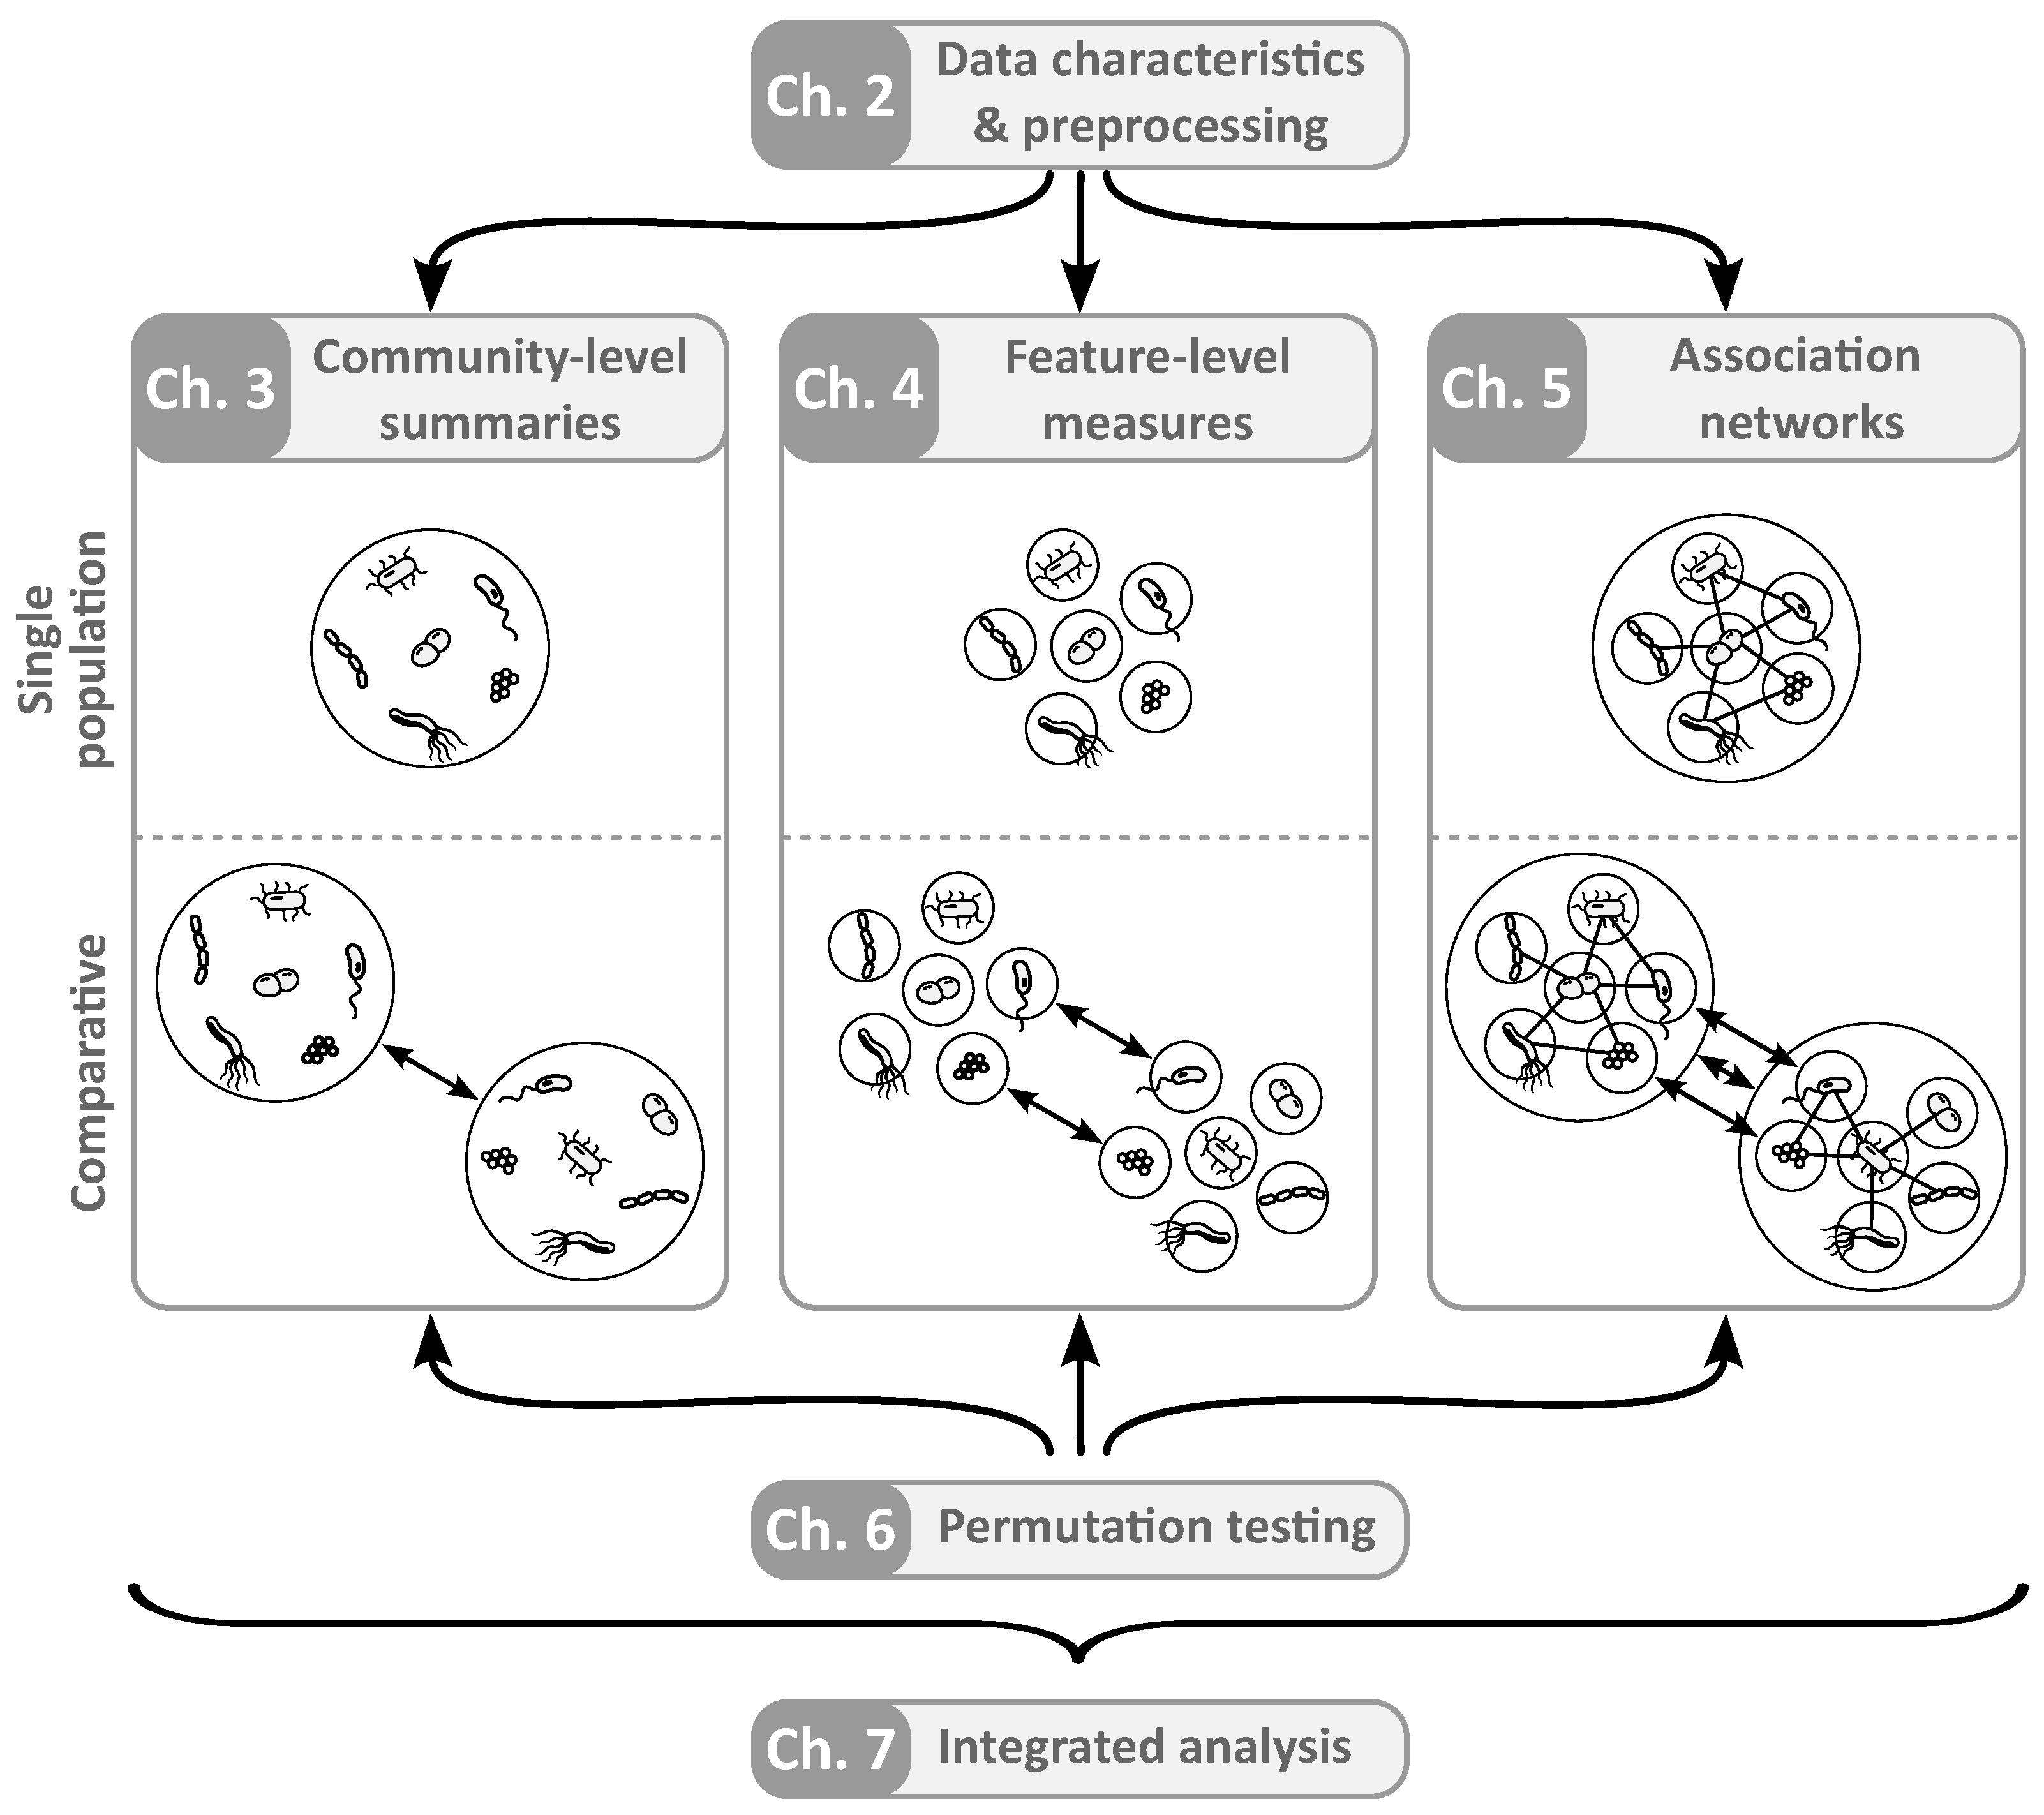
\includegraphics[width=\textwidth]{../ch01_introduction/figures/Intro_Figure.pdf}
	\caption{\textbf{Analysis targets and modes in microbiome studies.}
		The three columns represent the analysis targets considered in this thesis: community-level summaries, feature-level measures, and association networks. 
		The rows distinguish between single-population analysis and comparative analysis, where the latter focuses on differences between groups. 
		Data characteristics and preprocessing (Chapter~2) provide the foundation for all analysis targets. 
		Chapters~3 to 5 introduce methodological approaches for community-level summaries, feature-level measures, and association networks, respectively. 
		Permutation testing (Chapter~6) serves as a unifying inferential framework for comparative analyses across all targets. 
		Chapter~7 presents the complete analysis pipeline in an integrated real-data application.}
	\label{fig:levels_inference}
\end{figure}

\noindent\textbf{Community-level summaries.}
Community-level summaries describe aggregated properties of the microbial community. Typical quantities include measures of alpha diversity, such as richness or the Shannon index, as well as measures of beta diversity that quantify dissimilarity between samples. Ordination techniques provide low-dimensional representations of between-sample variation and facilitate exploratory analysis of community structure. In comparative settings, these summaries are used to assess whether global community characteristics differ between groups. 

\noindent\textbf{Feature-level measures.}
Feature-level measures characterize individual microbial taxa. 
In the single-population setting, this includes summaries of taxon abundances, prevalence patterns, and distributional characteristics within a cohort. In comparative settings, the objective is to quantify differences in abundance or distribution between groups or to assess associations with external covariates. Common approaches include differential abundance analysis, differential distribution testing, and regression-based modeling. All these methods operate at a marginal resolution, where each taxon is considered separately.

\noindent\textbf{Association networks.}
Association networks model relationships between microbial taxa. 
The primary object is a network whose edges encode statistical relationships, such as associations or conditional dependencies, between pairs of taxa. 
This relational representation gives rise to quantities at two complementary scales. 
On the one hand, node-level characteristics, such as centrality measures, describe the relative importance or role of individual taxa within the network. 
On the other hand, global network summaries, such as average path length or clustering coefficients, capture structural properties of the community as a whole. 
Association networks thus provide an explicitly relational perspective that links feature-level characteristics with community-level structure. 
As with the other analysis targets, network-based analyses can be performed within a single population or comparatively across groups, for example by assessing differences in network topology or in individual edges.


%====================================
\section{Permutation testing as a unifying approach}
\label{sec:intro:permutation}
%====================================

Across the different analysis targets introduced in the previous section, a common challenge arises in comparative settings: 
for many quantities of interest in microbiome analysis, the sampling distribution under the null hypothesis is analytically intractable or poorly approximated by classical parametric models. 
This difficulty is a direct consequence of the structural characteristics of microbiome data, including compositional constraints, sparsity, high dimensionality, and the use of complex transformations and derived statistics.

Permutation testing provides a general and flexible approach for hypothesis testing in such situations \citep{fisher1935design, good2005permutation}. Rather than relying on a parametric distribution, permutation tests approximate the null distribution by recomputing the test statistic under rearrangements of the data that preserve the null hypothesis. Their validity relies on exchangeability of the observations under the null hypothesis, which must be assessed with respect to the study design and the chosen permutation scheme \citep{good2005permutation}. Permutation tests are therefore useful in settings where classical distributional assumptions are difficult to justify.
Importantly, the relevance of permutation testing extends across all analysis targets considered in this thesis.

For community-level summaries, commonly used quantities such as alpha-diversity indices and between-sample dissimilarities often lack convenient parametric reference distributions. Group comparisons are therefore frequently based on nonparametric procedures. For example, PERMANOVA uses permutations of a distance-based test statistic to assess evidence for differences in multivariate community composition between groups \citep{anderson2001new}.

At the feature level, differential abundance and distribution analyses often involve sparse and discrete data, compositional transformations, or complex test statistics. In such settings, simple analytical reference distributions may be unavailable or may provide only an inadequate approximation to the null distribution.
Permutation-based approaches provide a robust alternative by directly approximating the null distribution of the chosen test statistic, regardless of its analytical form.

For association networks, permutation testing plays a central role in comparative analyses, as network characteristics typically lack tractable sampling distributions.
Permutation procedures are commonly used to assess differences in network structure, particularly for global network summaries and node-level characteristics whose sampling distributions are analytically intractable. Depending on the association measure and target of inference, edge-wise comparisons may alternatively be based on parametric or resampling-based procedures.

Taken together, permutation testing provides a unifying approach for hypothesis testing in comparative microbiome analyses across all considered targets. 
This central role motivates the methodological developments presented in Chapter~\ref{ch:permapprox}, where limitations of permutation-based testing under finite computational budgets are addressed and improved $p$-value approximation methods are developed.

%====================================
\section{Main contributions}
\label{sec:intro:contributions}
%====================================

At first glance, the methodological focus of this thesis may appear somewhat unexpected. 
Why concentrate on two seemingly distinct topics, namely microbial network analysis and permutation-based hypothesis testing? 
The former is a specialized tool within microbiome research, while the latter is a general statistical technique with applications far beyond this field. 
However, as will become apparent, both topics emerge naturally from the analytical challenges posed by microbiome data and are closely connected within comparative analysis workflows.

\subsubsection*{First contribution: a unified framework for microbial network analysis}
The focus on network analysis is perhaps the more intuitive of the two. 
Over the past decade, association networks have become a widely used exploratory tool for investigating relationships between microbial taxa and are increasingly incorporated into microbiome analysis workflows \citep{faust2021open}. 
At the same time, the literature reveals a lack of standardization, with microbial networks being constructed in many different ways and reflecting a wide range of methodological choices \citep{weiss2017normalization, kurtz2015sparse, ullmann2023overoptimism}. 
Their construction is inherently a multi-step procedure, involving preprocessing, association estimation, sparsification, and the computation of network characteristics. 
For each of these steps, a variety of methods exist.
Normalization strategies differ in their treatment of library size and compositional effects \citep{mcmurdie2014waste,mcknight2019methods,badri2020shrinkage}; compositionally aware association measures range from correlation-based methods to conditional-dependence approaches that can account for latent factors \citep{friedman2012inferring,quinn2017propr,kurtz2015sparse,kurtz2019disentangling}; and sparsification techniques include thresholding, shrinkage, and penalized likelihood procedures \citep{schafer2005shrinkage,meinshausen2006highdimensional,friedman2008sparse}. 

At the time of the original \texttt{NetCoMi} development, these methods were typically implemented in separate software packages and designed for specific components of the workflow rather than for integrated end-to-end analysis \citep{peschel2021netcomi}. Researchers therefore often had to assemble multiple methods in an ad hoc manner, limiting reproducibility and accessibility, especially for non-expert users.

To address these issues, the first methodological contribution of this thesis is the development of a unified framework for microbial network analysis. 
This framework is implemented in the \texttt{NetCoMi} \texttt{R} package \citep{peschel2026netcomi} and was introduced in \citet{peschel2021netcomi}. 
It provides an integrated workflow that guides the user from count data to a fully constructed and analyzed network by combining preprocessing, association estimation, sparsification, and network characterization within a single framework, while allowing flexible choices among established methods at each step. 
In addition, the framework supports comparative analyses, enabling the construction and comparison of networks across groups within a common and reproducible analytical framework. 
The \texttt{NetCoMi} framework is accompanied by comprehensive documentation and tutorials and has been integrated into the \emph{Orchestrating Microbiome Analysis} (OMA) workflow \citep{borman2024orchestrating}, where network-based methods are embedded into a broader microbiome analysis pipeline. 
By integrating existing methodology into a coherent and user-friendly framework, \texttt{NetCoMi} improves reproducibility, transparency, and accessibility of network-based microbiome analysis.

\subsubsection*{Second contribution: improved $p$-value approximation in permutation testing}
The second focus of this thesis, permutation-based hypothesis testing, arises less directly but is closely tied to comparative network analysis. 
When comparing microbial networks across groups, differences in network characteristics are typically assessed using permutation tests, as the underlying test statistics do not admit tractable parametric distributions. 
However, in this setting, two fundamental challenges emerge.

First, microbiome data are often high-dimensional, and network construction itself is computationally demanding. 
As a consequence, only a limited number of permutations can be performed in practice. 
This leads to empirical $p$-values that lie on a coarse discrete grid, resulting in limited resolution in the tail of the distribution \citep{north2002note, phipson2010permutation}. 
After multiplicity adjustment, this limited resolution can prevent small effects from being distinguished and may render adjusted significance thresholds unattainable unless a substantially larger number of permutations is used \citep{phipson2010permutation, gilbert2005modified}..

Second, while approaches based on extreme value theory, in particular generalized Pareto distribution (GPD) approximations, have been proposed to address this limitation \citep{knijnenburg2009fewer, winkler2016faster}, their practical application raises additional challenges. 
In preliminary investigations, existing GPD-based methods could still produce zero $p$-values when a negative estimated shape parameter implied bounded fitted support and the observed test statistic lay at or beyond the resulting upper endpoint.
Moreover, GPD-based approximation involves several methodological choices, including threshold selection and parameter estimation, for which a wide range of approaches has been proposed in extreme-value analysis \citep{scarrott2012review, langousis2016threshold, bader2018automated}, while guidance tailored specifically to permutation-based p-value approximation remains limited.

The second methodological contribution of this thesis addresses these challenges by developing a robust framework for permutation $p$-value approximation. 
This methodology is introduced in \citet{peschel2026permapprox} and implemented in the \texttt{permApprox} \texttt{R} package \citep{peschel2025permapprox}. 
The proposed approach ensures strictly positive $p$-value estimates by incorporating a support constraint into the GPD fitting procedure, thereby avoiding zero $p$-values. 
In addition, it provides a principled workflow for threshold selection and parameter estimation. 
Its performance is systematically evaluated through extensive simulation studies, showing accurate and stable $p$-value approximation across the simulated settings considered under limited permutation budgets.

Although the motivation for this development originates from comparative network analysis, the resulting methodology is formulated in a general way. 
It is applicable to permutation testing problems beyond network analysis and is relevant whenever $p$-values must be estimated from a limited number of permutations. 
This generality is reflected in the applications presented in this thesis, where the approach is used not only for network comparisons but also for analyses at the community and feature levels.

\subsubsection*{Third contribution: integrated real-data analysis across analysis targets}
The third contribution of this thesis is an integrated real-data analysis based on infant gut microbiome data from the PASTURE cohort \citep{vonmutius2006pasture}. It combines community-level summaries, feature-level comparisons, and association-network analyses within a coherent workflow. The analysis illustrates how complementary perspectives can yield distinct, but jointly informative, insights: taxa exhibiting marginal abundance differences are not necessarily central within association networks, and differential associations may occur without pronounced marginal group differences. By applying permutation-based procedures across the analysis pipeline and refining the resulting $p$-values with \texttt{permApprox}, the application also demonstrates the practical connection between the two methodological contributions of this thesis.

\subsubsection*{Reproducibility}
The code, analysis material, and figures accompanying this thesis are available in a GitHub repository archived on Zenodo \citep{Peschel2026thesisRepo}. The repository is structured by thesis chapter. Each chapter is represented by a corresponding folder containing the material used to generate or reproduce the reported results, tables, and figures. For chapters without accompanying analysis scripts, the corresponding folder contains the graphical material shown in the thesis. Large intermediate files from simulation studies are not included in all cases, but can be regenerated by rerunning the corresponding scripts provided in the repository.

Together, these contributions provide both methodological and practical advances for comparative microbiome research, linking workflow integration, permutation-based hypothesis testing, and applied analysis within a unified framework.

%====================================
\section{Thesis outline}
\label{sec:intro:structure}
%====================================

This dissertation follows a monograph structure that combines methodological development with applied microbiome data analysis.

\textbf{Chapter 2} formalizes microbiome sequencing data as statistical objects. It characterizes key properties of high-throughput sequencing data, including compositionality, sparsity, and high dimensionality, thereby establishing the foundations for the subsequent chapters.

\textbf{Chapter 3} introduces methods for community-level summaries. It presents commonly used measures such as alpha and beta diversity, along with ordination techniques, and discusses their use in descriptive and comparative analyses of microbial communities.

\textbf{Chapter 4} focuses on feature-level measures. It reviews approaches for analyzing individual taxa, including differential abundance and distributional analyses, and discusses statistical challenges arising from compositionality and sparsity.

\textbf{Chapter 5} focuses on association networks and presents the first methodological contribution of this thesis: the \texttt{NetCoMi} framework. 
It reviews existing approaches and introduces a unified workflow that integrates network construction, characterization, and comparison. 
Practical challenges arising from the implementation and combination of different methods are discussed throughout the chapter.

\textbf{Chapter 6} presents the second methodological contribution, a framework for accurate permutation $p$-value approximation under limited permutation budgets. It introduces the constrained tail-modeling approach, develops the associated workflow, and evaluates its performance in extensive simulation studies.

\textbf{Chapter 7} demonstrates the integration of the different analysis targets in a real-data application. Using a cohort study, it combines community-level summaries, feature-level measures, and association networks within a coherent analysis pipeline.

\textbf{Chapter 8} concludes the thesis with a discussion of the methodological contributions, their practical implications, and directions for future research.


Notation and abbreviations used throughout the thesis are summarized in Appendix~\ref{app:notation}. Chapter-specific notation is introduced locally where needed. In particular, Chapter~\ref{ch:permapprox} contains a dedicated overview for permutation testing and GPD tail modeling.

% !TeX root = ../thesis.tex

%%%%%%%%%%%%%%%%%%%%%%%%%%%%%%%%%%%%%%%%%%
\thesischapter[ch:microbiome][0.9\textwidth]
  {``Microbiome Datasets Are Compositional: And This Is Not Optional''}
  {--- G. B. Gloor, J. M. Macklaim, V. Pawlowsky-Glahn, and J. J. Egozcue, 2017}
  {Microbiome data as statistical objects}
\nocite{gloor2017microbiome}
\chapterabstract{This chapter formalizes microbiome sequencing data as statistical objects and describes the structural properties that shape downstream analyses. It introduces how sequencing experiments give rise to count matrices and discusses why compositionality, sparsity, heterogeneous library sizes, overdispersion, and high dimensionality challenge standard statistical methods. The chapter then reviews key preprocessing choices, including aggregation, filtering, library-size adjustment, zero handling, and transformation, and discusses their implications for downstream inference.}
\chaptercontents
%%%%%%%%%%%%%%%%%%%%%%%%%%%%%%%%%%%%%%%%%%

%%%%%%%%%%%%%%%%%%%%%%%%%%%%%%%%%%%%%
\section{Introduction}
\label{sec:2micro:introduction}
%%%%%%%%%%%%%%%%%%%%%%%%%%%%%%%%%%%%%

Microbiome sequencing experiments produce data that are biologically rich yet statistically constrained. Before turning to specific analysis targets, it is therefore necessary to clarify what kind of mathematical objects microbiome data represent and which structural properties characterize them. This chapter formalizes microbiome count data as high-dimensional, compositional, and sparse data objects arising from complex sampling processes. We begin by outlining how sequencing technologies give rise to count matrices and associated metadata. We then examine the key statistical characteristics of these data, including compositionality, library size variability, sparsity, overdispersion, and high dimensionality. Finally, we discuss common preprocessing steps and their implications for downstream analysis. The purpose of this chapter is not to introduce new methodology, but to establish the statistical and geometric foundations on which the analyses and methodological developments in later chapters are built.

%%%%%%%%%%%%%%%%%%%%%%%%%%%%%%%%%%%%%
\section{From sequencing reads to count matrices}
\label{micro:count_data}
%%%%%%%%%%%%%%%%%%%%%%%%%%%%%%%%%%%%%

High-throughput sequencing technologies enable the culture-independent characterization of microbial communities across diverse environments \citep{caporaso2012ultrahighthroughput,shendure2017dna}. In microbiome research, two principal strategies are commonly employed. Marker-gene amplicon sequencing targets specific conserved genomic regions to infer taxonomic composition, whereas shotgun metagenomic sequencing fragments and sequences a broad collection of DNA fragments extracted from a sample, thereby providing information on both taxonomic composition and functional potential \citep{sharpton2014introduction,quince2017shotgun}.

In bacterial and archaeal studies, marker-gene approaches most commonly target the 16S ribosomal RNA (rRNA) gene \citep{sanschagrin2014nextgeneration}. The 16S rRNA gene encodes a structural component of the small ribosomal subunit and is universally present in prokaryotes. Its sequence consists of highly conserved regions interspersed with hypervariable regions. The conserved regions enable the design of universal primers for polymerase chain reaction (PCR) amplification, while the variable regions accumulate mutations that reflect evolutionary divergence and thus provide taxonomic information \citep{chakravorty2007detailed}. The phylogenetic relevance of rRNA sequences and their role in reconstructing evolutionary relationships were systematically established by \citet{woese1987bacterial}, laying the foundation for modern microbial taxonomy. For fungal communities, the internal transcribed spacer (ITS) region serves as a widely accepted marker due to its higher interspecific variability \citep{schoch2012nuclear}, while the 18S rRNA gene is frequently used for eukaryotic microorganisms \citep{hadziavdic2014characterization}.

A fundamental characteristic of standard marker-gene sequencing protocols is that they produce relative rather than absolute abundance measurements. Because sequencing depth is finite and the total number of reads per sample is limited, the observed counts reflect the proportion of sequencing effort allocated to each taxon rather than their actual microbial load \citep{gloor2017microbiome}. 

To address this limitation, quantitative microbiome profiling protocols have been proposed. These approaches either estimate total microbial load independently, for example via flow cytometry \citep{props2017absolute,vandeputte2017quantitative}, or introduce known internal standards prior to sequencing to enable calibration of observed counts \citep{lin2019quantitative,stammler2016adjusting}. While such strategies can provide valuable information on absolute microbial abundance, many microbiome datasets remain based solely on sequencing counts without independent absolute quantification.

Shotgun metagenomic sequencing differs from marker-gene sequencing in that it does not target a specific genomic region but instead sequences a broad collection of DNA fragments extracted from a sample. As a result, shotgun approaches allow simultaneous taxonomic and functional profiling at higher resolution \citep{quince2017shotgun}. Nevertheless, standard shotgun protocols also yield read counts constrained by total sequencing depth and therefore share the compositional characteristics of marker-gene data unless complemented by independent absolute quantification.

In this thesis, we primarily focus on marker-gene sequencing data, in particular 16S rRNA amplicon sequencing, which remains one of the most widely used approaches in host-associated microbiome research. The statistical challenges arising from compositional constraints, sparsity, and high dimensionality are prominent in such datasets, making them a natural setting for methodological development. Many of the inferential principles discussed later, however, extend to shotgun metagenomic data as well.

After bioinformatic preprocessing, sequencing reads are summarized into features. In amplicon sequencing workflows, this commonly includes quality control, denoising, and chimera removal. Depending on the bioinformatic pipeline, these features may correspond to amplicon sequence variants (ASVs), which resolve sequences at single-nucleotide resolution \citep{callahan2016dada2}, to operational taxonomic units (OTUs), or to genes or taxonomic groups at a specified rank. 

The resulting data are organized into a count matrix. 
In this thesis, $n$ denotes the number of samples and $p$ the number of taxa (features), so that the count matrix is defined as
\begin{equation}
\label{eq:micro:count_matrix}
    \mathbf{X} = (x_{ki}) \in \mathbb{N}_0^{n \times p}, 
    \quad k = 1, \dots, n, \; i = 1, \dots, p.
\end{equation}
Here, $x_{ki}$ denotes the number of reads assigned to taxon $i$ in sample $k$. 
The total number of reads observed in sample $k$,
\begin{equation}
	\label{eq:micro:library_size}
    m_k = \sum_{i=1}^{p} x_{ki},
\end{equation}
is commonly referred to as the \emph{library size}. 
In the microbiome literature, the term \emph{sequencing depth} is often used synonymously. 
Strictly speaking, sequencing depth refers to the intensity of sequencing effort applied to a sample, whereas library size denotes the realized total number of reads obtained. 
In this thesis, we use the term \emph{library size} to emphasize that $m_k$ is an observed data quantity.

In addition to the count matrix, microbiome studies typically include two further data components. 
First, a sample metadata table contains clinical, environmental, or \text{experimental} covariates for each sample, such as age, treatment group, or sampling location. 
Second, each feature (taxon) is accompanied by a taxonomic annotation that assigns it to hierarchical ranks such as phylum, class, order, family, genus, and species. 
This taxonomic table reflects the biological classification derived from sequence similarity or reference databases and enables aggregation of counts at different taxonomic levels.

The count matrix $\mathbf{X} \in \mathbb{N}_0^{n \times p}$ constitutes the primary statistical object underlying microbiome data analysis. Its properties are fundamentally shaped by the sequencing process, the aggregation of reads into features, and the compositional constraint imposed by finite library sizes. While the count matrix forms the basis for most quantitative analyses, metadata and taxonomic structure play a crucial role in interpretation, aggregation, and group comparisons.

%%%%%%%%%%%%%%%%%%%%%%%%%%%%%%%%%%%%%
\section{Characteristics of microbiome data}
\label{sec:2micro:characteristics}
%%%%%%%%%%%%%%%%%%%%%%%%%%%%%%%%%%%%%

\begin{figure}[H]
\centering
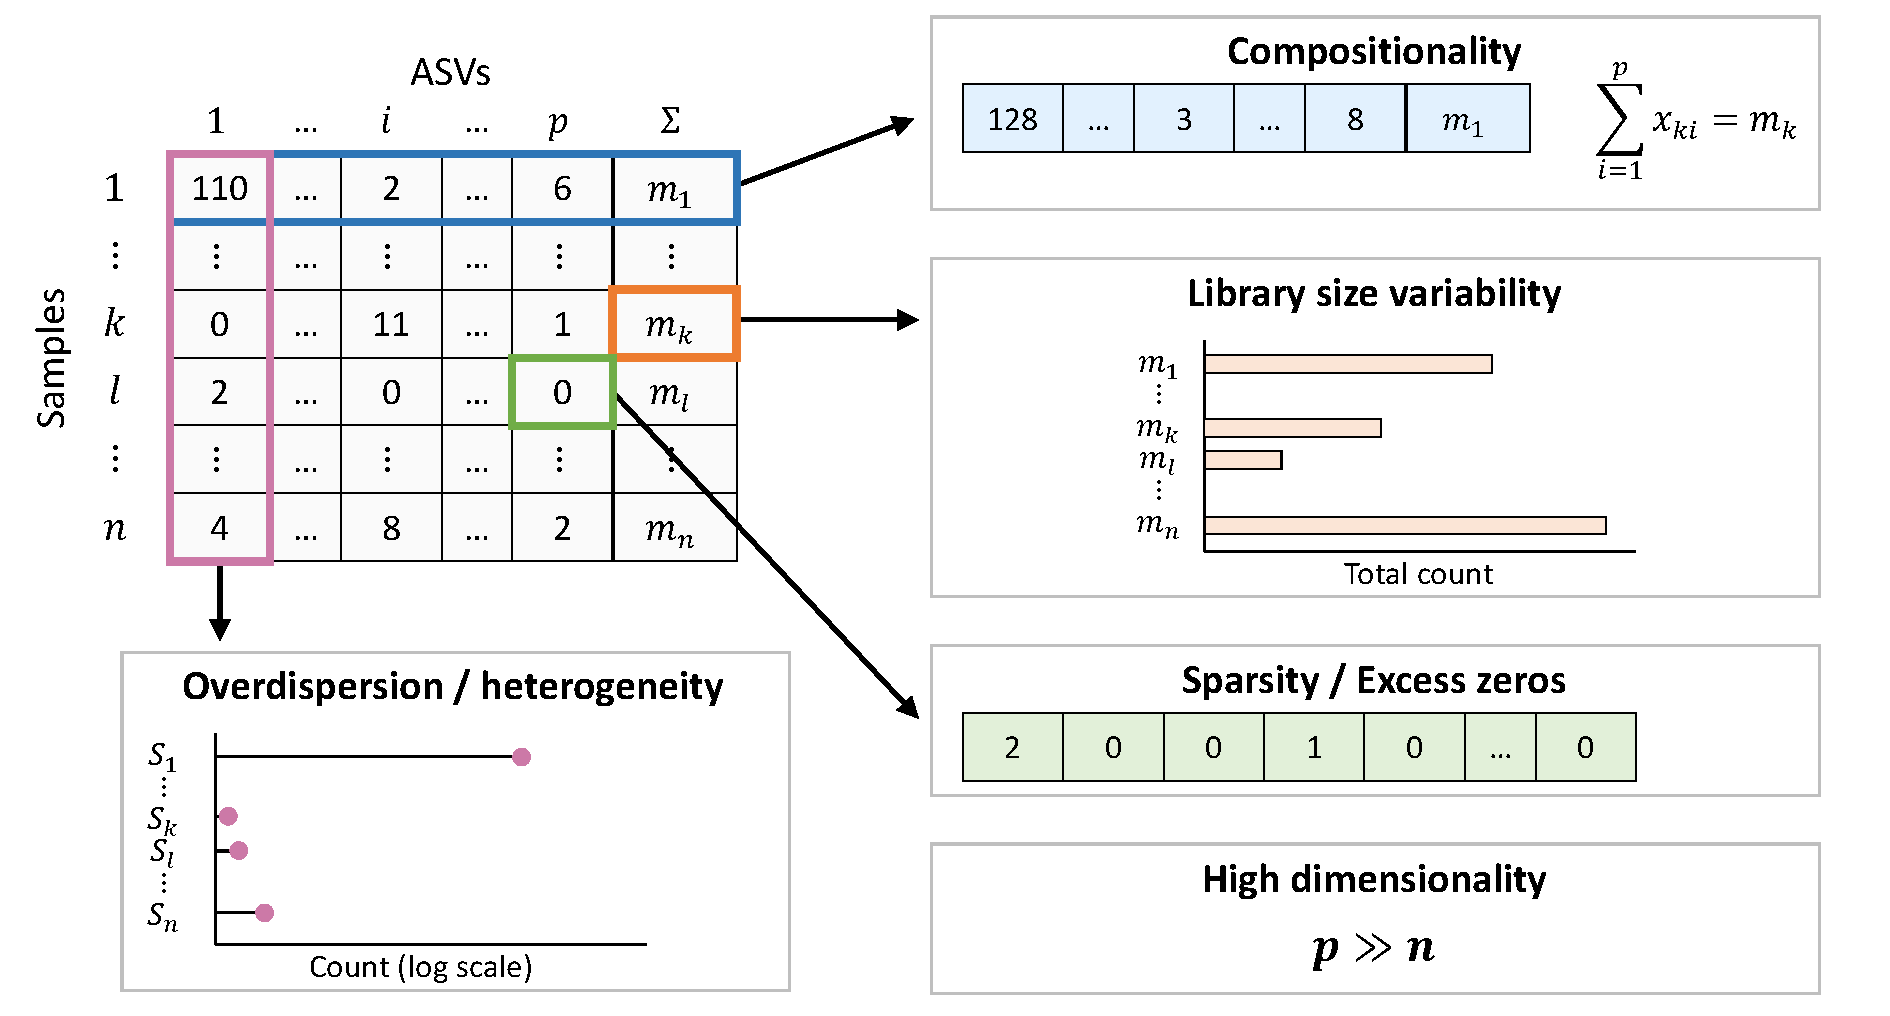
\includegraphics[width=\textwidth]{../ch02_microbiome_data/overview_figures/overview_characteristics.pdf}
\caption{\textbf{Overview of characteristic properties of microbiome count data.} The count matrix contains non-negative read counts for $n$ samples and $p$ taxa. Each sample is constrained by its library size $m_k$, leading to compositional structure. Library sizes vary across samples, many taxa contain zero counts, count distributions may be highly heterogeneous and overdispersed, and the number of taxa is often large relative to the number of samples. These properties motivate the preprocessing and modeling choices discussed throughout this chapter.}
\label{fig:2micro:overview_characteristics}
\end{figure}

Microbiome count matrices have several structural properties that distinguish them from unconstrained multivariate data matrices. These properties arise from the sequencing process, the aggregation of reads into microbial features, and the ecological structure of microbial communities. Figure~\ref{fig:2micro:overview_characteristics} provides an overview of the main characteristics discussed in this section. The entries of the count matrix are constrained by the sample-specific library size, library sizes vary between samples, many entries are zero, count distributions are heterogeneous and overdispersed, and the number of taxa is often large relative to the number of samples. Each of these aspects affects how microbiome data should be preprocessed, modeled, and interpreted.

%====================================
\subsection{Compositionality and induced dependence}
\label{sec:2micro:charact:compositionality}
%====================================

A defining structural property of microbiome sequencing data is their \emph{compositional} nature. 
Under typical high-throughput sequencing protocols, only a finite number of reads can be obtained from each sample \citep{gloor2017microbiome}. 
For each sample $k$, the total number of reads
\begin{equation}
    m_k = \sum_{i=1}^{p} x_{ki}
\end{equation}
is determined primarily by technical and experimental factors such as sequencing platform capacity, degree of multiplexing, PCR amplification efficiency, and DNA extraction efficiency, rather than by the absolute microbial load in the underlying biological environment \citep{nearing2021identifying}. 
Consequently, the observed counts $x_{ki}$ reflect the relative allocation of sequencing effort across taxa rather than their absolute abundances.

Conditional on the sample-specific library size $m_k$, the count vector $\mathbf{x}_k = (x_{k1}, \dots, x_{kp})^\top$ satisfies the constant-sum constraint
\begin{equation}
\sum_{i=1}^{p} x_{ki} = m_k,
\end{equation}
which restricts it to a $(p-1)$-dimensional affine subspace of $\mathbb{R}^{p}$.
This restriction is referred to as \emph{closure} and forms the foundation of compositional data analysis \citep{aitchison1982statistical,gloor2016its}. 
Importantly, closure is induced by the sampling mechanism itself and does not result from any subsequent normalization procedure.

Closure implies that the components of $\mathbf{x}_k$ cannot vary independently. 
Conditional on $m_k$, an increase in one component must be accompanied by a decrease in at least one other component, even if the corresponding taxa are biologically unrelated.
As a result, the count vector is identifiable only up to a positive scaling factor: absolute abundances cannot be recovered from sequencing data without additional external information. 
Inference is therefore restricted to relative quantities.

From a statistical perspective, compositionality implies that standard multivariate methods developed for unconstrained Euclidean data cannot be applied without modification. 
Because the components of $\mathbf{x}_k$ satisfy a linear constraint, the data exhibit inherent dependence induced by the constant-sum restriction. 
In particular, naive covariance and correlation estimates computed directly from raw counts may reflect this structural dependence rather than genuine biological associations. 
Thus, apparent negative correlations between taxa may arise purely as a mathematical consequence of closure rather than genuine biological interaction.

To address these issues, Aitchison developed a principled framework for the statistical analysis of compositional data based on log-ratio transformations \citep{aitchison1982statistical}. 
The central insight is that only relative information between components is meaningful in the presence of closure, and that this information is naturally captured by ratios between components. 
Log-ratio transformations embed compositional vectors into a $(p-1)$-dimensional Euclidean space, thereby enabling the application of conventional multivariate techniques while respecting the relative nature of the data.

Aitchison’s framework is grounded in two fundamental principles. 
The first is \emph{scale invariance}: statistical conclusions should remain unchanged under multiplication of all components of a composition by a positive constant, reflecting the fact that only relative information is observable. 
The second is \emph{subcompositional coherence}, which requires that inference based on a subset of components be consistent with that obtained from the full composition restricted to the same subset. 
These principles formalize the idea that compositional data carry only relative information and that analyses should not depend on arbitrary changes in total scale or on the presence of additional irrelevant components \citep{aitchison1982statistical,greenacre2023aitchisons}.

However, log-ratio transformations require strictly positive components, which is problematic in the presence of zero counts. 
The interplay between compositional structure and sparsity therefore introduces additional theoretical and methodological challenges that are discussed in the subsequent sections.

%====================================
\subsection{Library size variability}
\label{sec:2micro:charact:librarysize}
%====================================

While closure describes a within-sample constraint, the total number of counts varies considerably across samples within the same study. 
As introduced above, the library size
\[
m_k = \sum_{i=1}^{p} x_{ki}
\]
is primarily determined by technical and experimental factors rather than by the absolute microbial load in the biological specimen. In practice, the values $m_k$ often differ substantially across samples.

Causes for library size variability include differences in DNA extraction efficiency, amplification yield during polymerase chain reaction, sample multiplexing, and stochastic fluctuations during library preparation \citep{nearing2021identifying}. 
As a result, two samples with identical underlying community composition may exhibit different total read counts purely due to technical variation.

This heterogeneity has important statistical consequences. 
First, raw counts are not directly comparable across samples: even when two samples share identical underlying community composition, the sample with larger library size will produce larger observed counts. 
Differences in $m_k$ can therefore induce apparent differences in taxon abundances that are unrelated to biological variation.

\newpage
Second, sampling variability depends on library size. 
Samples with smaller library sizes provide less information about low-abundance taxa and are more prone to sampling zeros. 
Thus, the library size influences the resolution at which community composition is observed and interacts with sparsity and the occurrence of sampling zeros.

In many sequencing studies, library size is primarily a technical quantity that affects the scale and variability of observed counts. Unless independently calibrated, it should therefore not be interpreted directly as a measure of biological abundance.
Statistical analyses must therefore account for heterogeneous library size to avoid confounding biological differences with differences in sequencing effort. 
Approaches for handling library size variability are discussed in the preprocessing section.


%====================================
\subsection{Sparsity and excess zeros}
\label{sec:2micro:charact:sparsity}
%====================================

Beyond compositionality and heterogeneous library sizes, microbiome count data are characterized by pronounced sparsity and a high prevalence of zero counts. 
In typical datasets, a substantial proportion of entries in the count matrix $\mathbf{X}$ are equal to zero.

Sparsity reflects both the ecological structure of microbial communities and limitations of the measurement process.
Abundance distributions are typically highly uneven: a small number of taxa account for a large fraction of the total reads, whereas many taxa occur at low abundance or only in a subset of samples. 
Consequently, the empirical distribution of counts is strongly right-skewed, and rare taxa contribute disproportionately to the number of zero entries \citep{xia2024applied,li2015microbiome}.

Observed zeros in microbiome data are heterogeneous and may arise through different mechanisms. 
Following terminology from compositional data analysis \citep{martin-fernandez2003dealing,martin2011dealing,filzmoser2018applied}, one may distinguish:

\begin{itemize}
    \item \emph{Structural zeros}, corresponding to true absence of a taxon in a given environment;
    \item \emph{Rounded zeros}, where a taxon is present at very low abundance but is not detected by the measurement process;
    \item \emph{Sampling zeros}, which arise because sequencing produces a finite random sample of reads, so that taxa with low underlying abundance may not be observed in a given sample.
\end{itemize}

While these mechanisms differ conceptually, they cannot be distinguished from the observed count matrix alone. 
In practice, many zeros reflect a combination of low underlying abundance and finite sampling depth, particularly in samples with small library sizes.

From a statistical perspective, sparsity and excess zeros have several important implications. 
First, they complicate transformations and modeling strategies that require strictly positive values, such as log-ratio representations. 
Second, taxa observed in only a small subset of samples contribute limited information for the estimation of means, variances, or pairwise associations. 
For rare taxa, the number of samples contributing informative non-zero observations can be substantially smaller than the nominal sample size $n$ \citep{kurtz2015sparse}, leading to increased estimator variability and reduced stability in downstream analyses.

Moreover, sparsity interacts with compositionality and library size variability. 
Low-abundance taxa are particularly sensitive to fluctuations in sequencing depth and are more prone to sampling zeros, amplifying apparent differences across samples. 
As a result, preprocessing decisions such as filtering rare taxa or handling zeros can have substantial influence on subsequent statistical inference.

%====================================
\subsection{Overdispersion and heterogeneity}
\label{sec:2micro:charact:overdispersion}
%====================================

In addition to sparsity and excess zeros, microbiome count data typically exhibit substantial variability across samples that exceeds what would be expected under simple count models. 
This phenomenon is commonly referred to as \emph{overdispersion} \citep{xia2024applied,weiss2017normalization}.

Classical models for count data provide a useful reference point. 
Under an independent Poisson model, the variance of each taxon count equals its mean. 
Similarly, under a multinomial sampling model conditional on the library size $m_k$, the variance structure is fully determined by $m_k$ and the underlying relative abundances. 
Both formulations imply a restrictive relationship between mean and variance.

Empirical microbiome data frequently exhibit variability that exceeds the variance implied by simple Poisson or multinomial sampling models with fixed underlying abundance parameters. 
Even after accounting for library size, the observed variability of taxon counts across samples often exceeds that predicted by Poisson or multinomial sampling models with fixed underlying abundance parameters.
This additional variability may reflect heterogeneity in underlying relative abundances across samples, arising from biological variation, technical effects, or both \citep{weiss2017normalization,xia2024applied}.

Ignoring overdispersion can lead to underestimated variance, anticonservative hypothesis tests, and inflated false positive rates \citep{anders2010differential,robinson2010edger}. In high-dimensional settings, heterogeneous variance structures further complicate covariance and association estimation, particularly for low-abundance taxa.

To accommodate overdispersion, models with explicit dispersion parameters, such as negative binomial or Dirichlet-multinomial formulations, are commonly employed. 
Alternatively, variance-stabilizing transformations may be applied prior to downstream analysis. 
The choice of strategy depends on the inferential objective and is discussed in later sections.

%====================================
\subsection{High dimensionality}
\label{sec:2micro:charact:highdim}
%====================================

Microbiome feature tables, particularly at fine taxonomic resolution, often contain a large number of taxa $p$ relative to the number of samples $n$, resulting in the so-called ``large $p$, small $n$'' regime \citep{xia2024applied}. In this setting, classical statistical procedures developed for the $p<n$ regime are no longer directly applicable.

When $p$ is comparable to or exceeds $n$, empirical covariance matrices become singular or ill-conditioned, and least-squares estimators are either non-unique or exhibit high variance. 
Regression models, multivariate hypothesis tests, and dimension-reduction techniques may therefore become unstable without additional structural assumptions or regularization.

High dimensionality also increases the burden of multiple testing at the feature level and inflates the number of potential pairwise relationships when studying dependence structures. 
As a consequence, statistical inference in microbiome studies typically requires penalization, dimension reduction, or other regularized approaches tailored to high-dimensional data.

Taken together, compositionality, heterogeneous library sizes, sparsity, overdispersion, and high dimensionality define a statistical regime that differs fundamentally from classical multivariate data settings and requires a dedicated statistical methodology.

%====================================
\subsection{Consequences for statistical analysis}
\label{sec:2micro:charact:consequences}
%====================================

The structural properties discussed above are not merely technical nuisances but fundamentally shape the geometry of the sample space and the validity of downstream analyses. Compositionality implies that observations reside in the simplex rather than in unconstrained Euclidean space \citep{aitchison1986statistical}, sparsity gives rise to highly skewed count distributions with many zero observations, and high dimensionality challenges classical statistical procedures when the number of features is comparable to or exceeds the number of samples, leading, for instance, to unstable covariance estimation and non-unique unregularized regression estimates \citep{xia2024applied}.

Taken together, these characteristics restrict the applicability of standard parametric modeling strategies and complicate the construction of reliable reference distributions for hypothesis testing. They affect all three analysis targets considered in this thesis: community-level summaries, feature-level measures, and association networks. In comparative analyses, resampling-based procedures such as permutation tests therefore become attractive whenever analytic null distributions are unavailable or unreliable, provided that the permutation scheme is compatible with the study design and the null hypothesis. However, as discussed in Chapter~\ref{ch:permapprox}, permutation testing also has intrinsic limitations under finite computational budgets. The statistical developments of this thesis therefore originate directly from the structural constraints formalized in the present chapter.

%%%%%%%%%%%%%%%%%%%%%%%%%%%%%%%%%%%%%
\section{Taxonomic aggregation}
\label{sec:2micro:aggregation}
%%%%%%%%%%%%%%%%%%%%%%%%%%%%%%%%%%%%%

\begin{figure}[H]
\centering
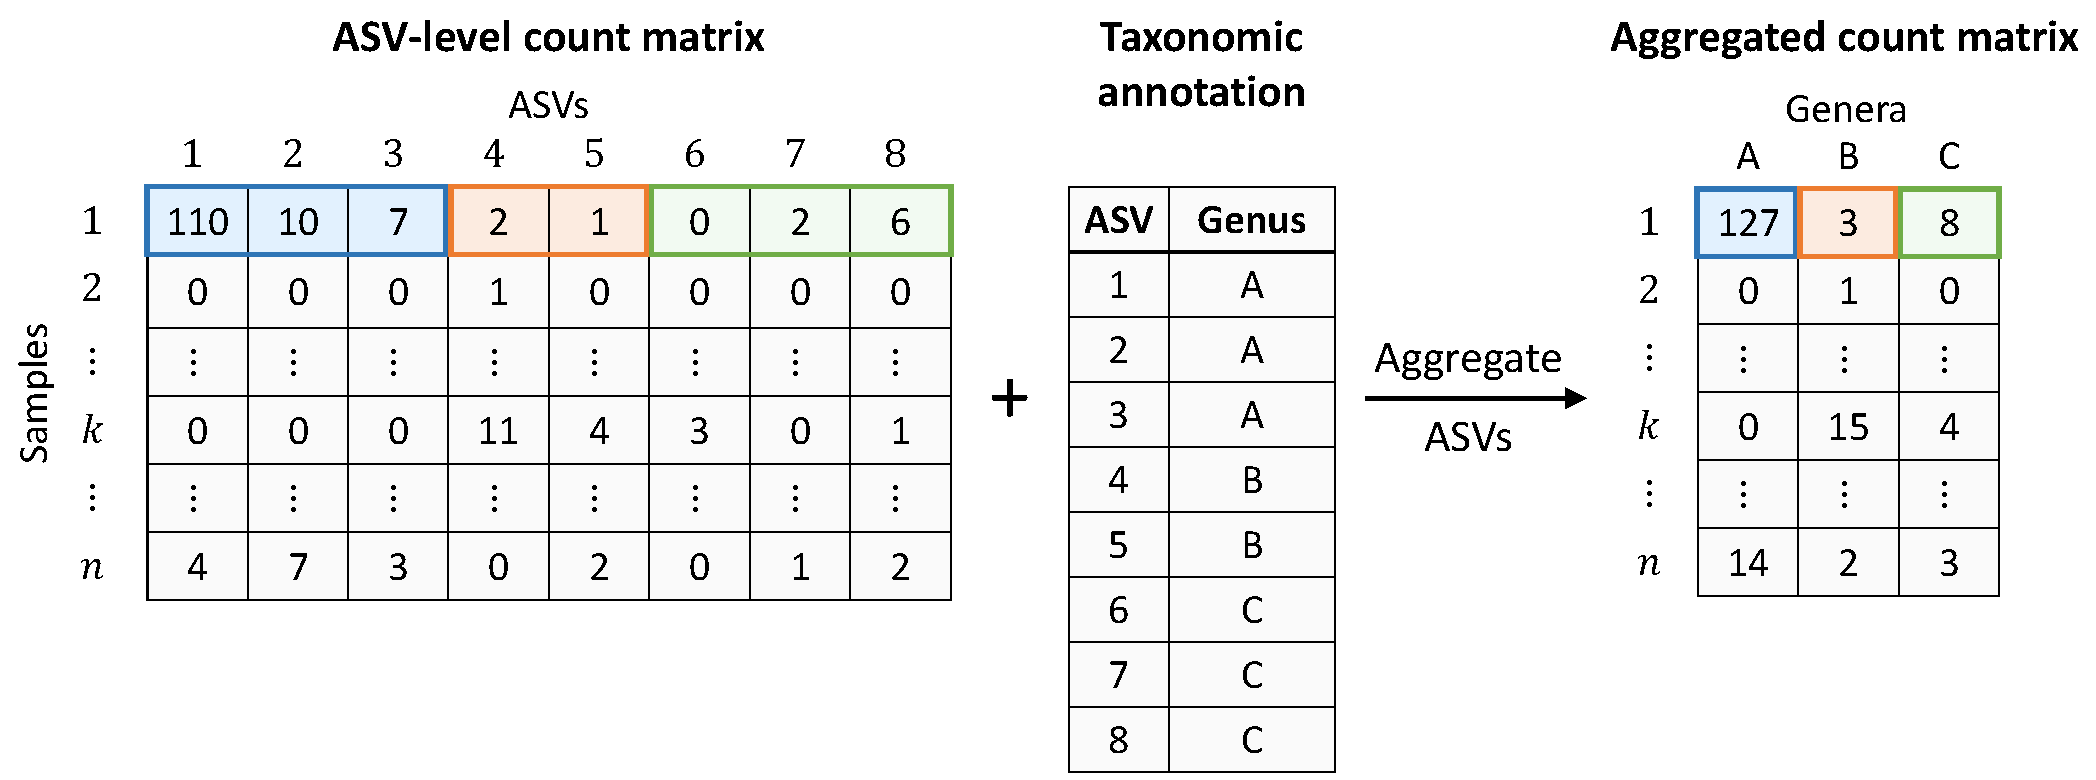
\includegraphics[width=\textwidth]{../ch02_microbiome_data/overview_figures/overview_aggregation.pdf}
\caption{\textbf{Overview of taxonomic aggregation.} The figure illustrates the aggregation of an ASV-level count matrix to genus level using the corresponding taxonomic annotation. The taxonomic table assigns each ASV to a genus, here denoted by A, B, and C. ASVs assigned to the same genus are combined by summing their counts within each sample, resulting in an aggregated count matrix with one column per genus.}
\label{fig:2micro:overview_aggregation}
\end{figure}

After primary bioinformatic processing, microbiome sequencing data are typically available as a feature table together with sample metadata and taxonomic annotations. In this thesis, we assume that read-level processing steps such as quality filtering, denoising, chimera removal, and feature inference have already been completed, for example using pipelines such as DADA2 \citep{callahan2016dada2}. The statistical analysis therefore starts from the resulting count matrix, and preprocessing refers to operations applied to this matrix before descriptive analysis, modeling, or hypothesis testing.

Before choosing the taxonomic resolution of the analysis, a minimal preliminary cleanup is usually applied to remove empty rows and columns from the selected data set. Samples with zero total counts cannot contribute to compositional analyses, and taxa with zero total counts in the retained samples contain no information for the corresponding analysis cohort. This preliminary removal of empty samples or taxa should be distinguished from abundance- or prevalence-based filtering, which is discussed in Section~\ref{sec:2micro:filtering} and is typically applied after the analysis feature space has been defined.

A common next preprocessing decision concerns the taxonomic resolution at which the microbiome is represented. Taxonomic aggregation combines lower-level features into higher-level taxonomic units according to their annotation. Figure~\ref{fig:2micro:overview_aggregation} illustrates this step for an ASV-level count matrix that is aggregated to genus level. The resulting matrix defines the feature space for the subsequent analyses.

Taxonomic aggregation is commonly performed by summing ASV- or OTU-level counts to genus, family, or phylum level. If $g(i)$ denotes the taxonomic group assigned to feature $i$, the aggregated count for group $h$ in sample $k$ is given by
\begin{equation}
x^{\mathrm{agg}}_{kh} = \sum_{i:g(i)=h} x_{ki}.
\label{eq:2micro:taxonomic_aggregation}
\end{equation}
The resulting count matrix has typically fewer columns than the original matrix and represents the microbiome at a coarser taxonomic resolution. In practical microbiome workflows in R, this operation is often implemented using the function \texttt{tax\_glom()} from the \texttt{phyloseq} package, which agglomerates features according to a selected taxonomic rank \citep{mcmurdie2013phyloseq}. The result depends on the available taxonomic annotation and on how unresolved assignments are handled. Such features may be retained as unclassified groups, aggregated at the lowest reliably assigned rank, or excluded; these choices should be reported because they affect the resulting feature space and downstream analyses.

Aggregation can reduce dimensionality and sparsity and may improve interpretability, especially when the original count matrix contains many rare ASVs or OTUs. It can also improve the numerical stability of downstream analyses, because higher-level taxa are often observed in more samples and with larger counts. At the same time, aggregation changes the biological and statistical object under investigation. A genus-level feature is not equivalent to a single organism, but represents the combined signal of all lower-level features assigned to that genus. Heterogeneous behavior within a taxonomic group may therefore be masked. For example, two ASVs assigned to the same genus may show opposite group-specific patterns, which can cancel after aggregation.

Taxonomic aggregation is therefore not merely a visualization decision, but determines the feature space and the hypotheses addressed by subsequent analyses. Testing at ASV level concerns differences in individual sequence variants between groups, whereas genus-level analysis concerns differences in the aggregated genus-level feature formed by the assigned variants. Similarly, community-level dissimilarities, feature-level test statistics, and estimated association networks may all change after aggregation, because summing lower-level features alters both marginal abundance patterns and pairwise relationships between the retained features. The chosen taxonomic level therefore defines the basis for subsequent filtering, normalization, zero handling, transformation, and inference.

However, aggregation to a single fixed rank is not equally suitable for all microbiome analyses. Some methods explicitly use the taxonomic hierarchy or combine information across multiple taxonomic levels. For example, tree-aggregated predictive modeling uses the phylogenetic or taxonomic tree to construct predictors at multiple aggregation levels and selects among them during model fitting \citep{bien2021treeaggregated}. In such settings, reducing the data to one preselected taxonomic rank may discard information that the method is designed to exploit. In the analyses presented in this thesis, however, the feature space is fixed before downstream preprocessing and inference. Unless stated otherwise, the application analyses are performed at genus level, so that subsequent filtering, normalization, zero handling, transformation, and statistical testing are applied to genus-level count matrices.


%%%%%%%%%%%%%%%%%%%%%%%%%%%%%%%%%%%%%
\section{Filtering of samples and taxa}
\label{sec:2micro:filtering}
%%%%%%%%%%%%%%%%%%%%%%%%%%%%%%%%%%%%%

\begin{figure}[H]
\centering
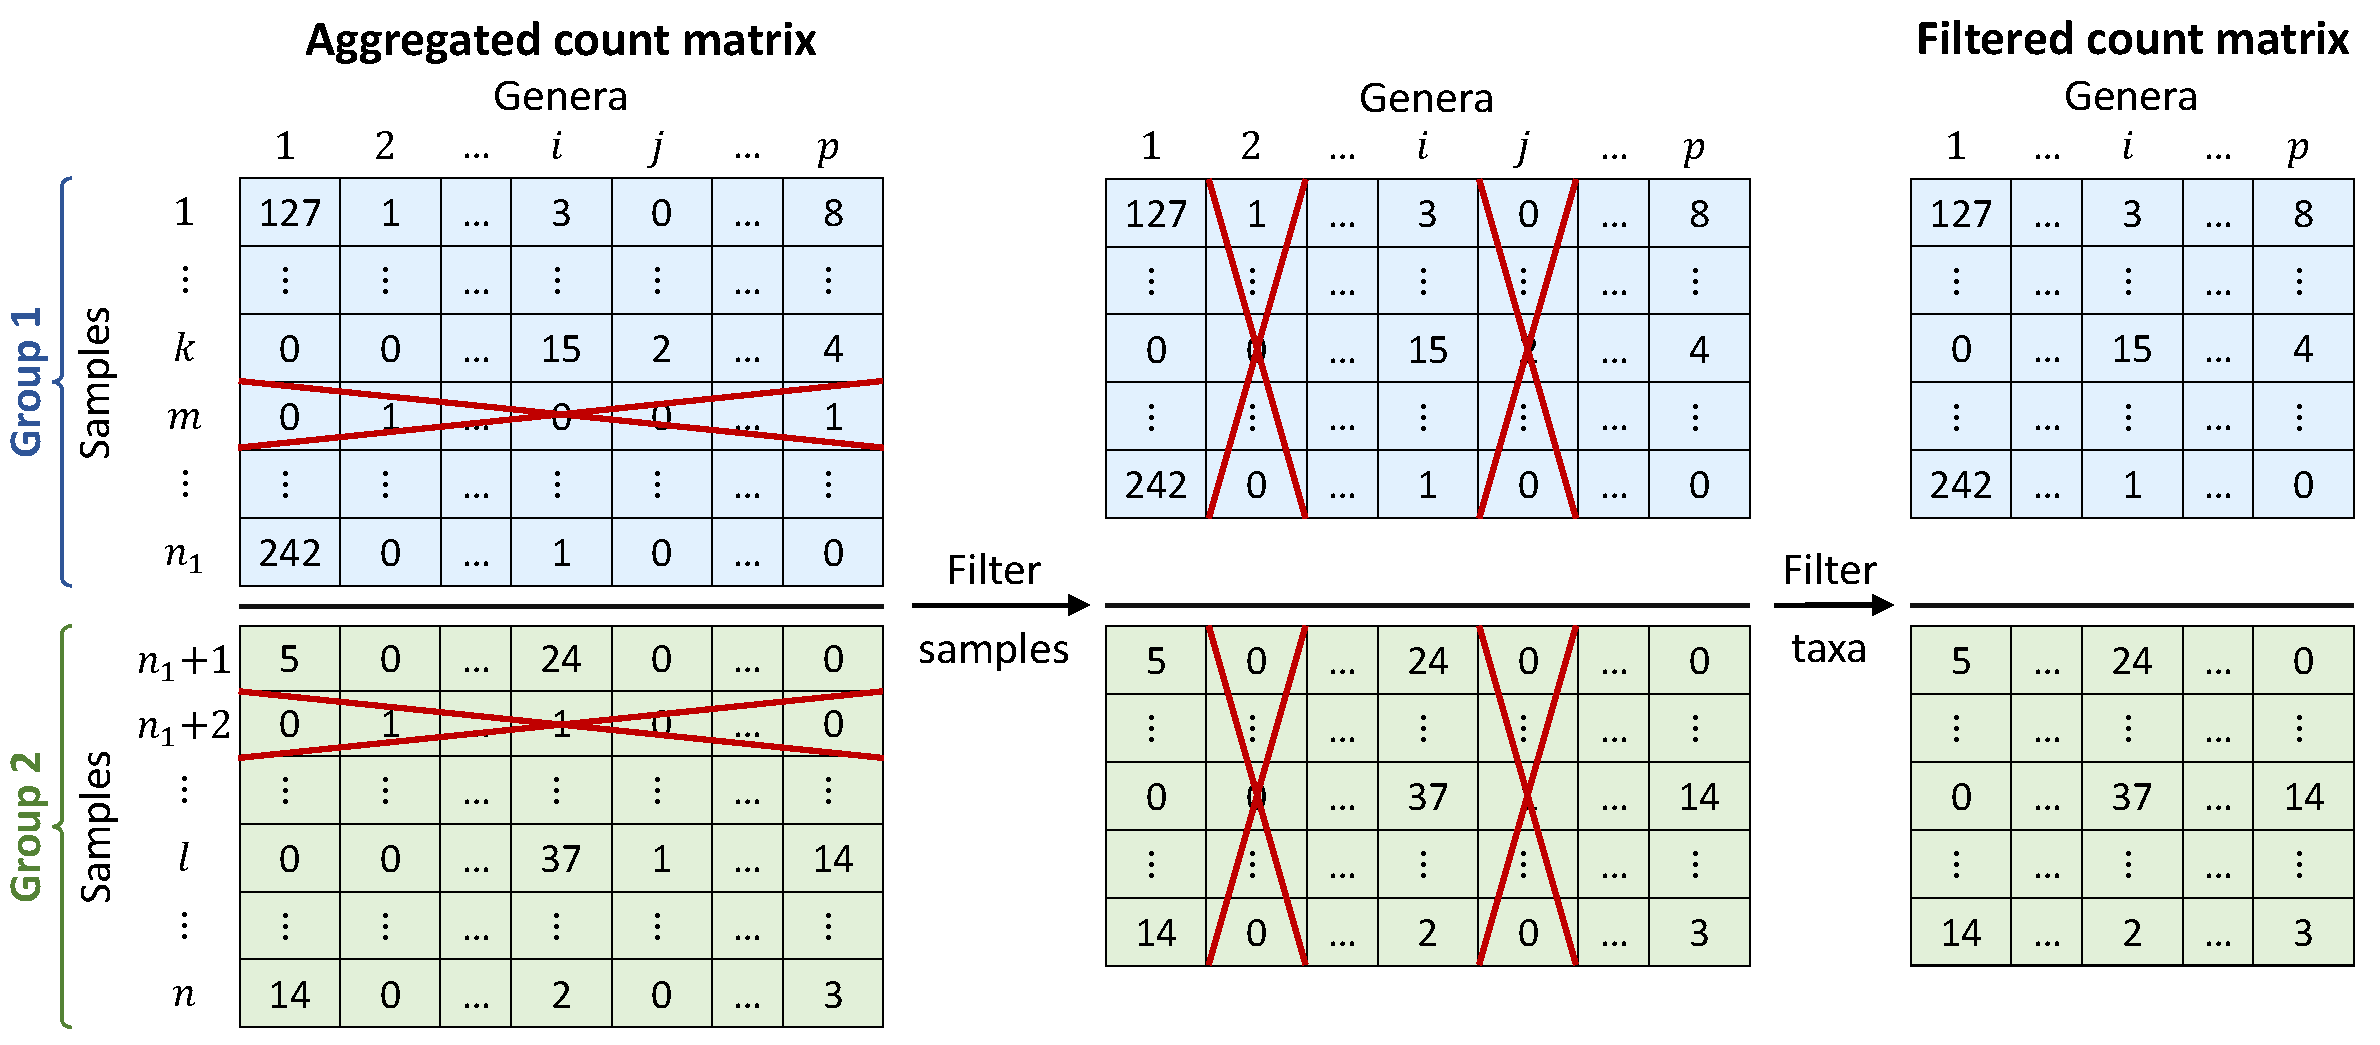
\includegraphics[width=\textwidth]{../ch02_microbiome_data/overview_figures/overview_filtering.pdf}
\caption{\textbf{Overview of sample and taxa filtering.} The figure illustrates filtering of an aggregated microbiome count matrix at genus level. Samples may be removed according to sample-level criteria, such as insufficient sequencing depth, missing metadata, or analysis eligibility. Genera may be removed according to feature-level criteria, such as low abundance, low prevalence, or insufficient variability. The two colored sample blocks represent two groups and are shown for consistency with later comparative analyses. Filtering criteria may be evaluated on the pooled data set or separately within groups, which can lead to different retained samples or genera.}
\label{fig:2micro:overview_filtering}
\end{figure}

After the taxonomic resolution of the analysis has been chosen, additional filtering may be applied to remove samples or taxa that provide little reliable information for the downstream analysis. Figure~\ref{fig:2micro:overview_filtering} illustrates this step for a count matrix represented at the selected taxonomic level. In contrast to the preliminary removal of empty rows and columns described in Section~\ref{sec:2micro:aggregation}, filtering in this section refers to analysis-level criteria such as sequencing depth, abundance, prevalence, and variability \citep{xia2024applied,weiss2017normalization}. Such filtering can improve numerical stability, reduce sparsity, and make the resulting feature space more interpretable. At the same time, it changes the data object under study and may influence downstream inference. Filtering should therefore be viewed not as a purely technical cleaning step, but as an analysis decision that needs to be reported and justified.

From this point onward, the overview figures display two sample groups, reflecting the comparative focus of later chapters. The grouping is included for visual consistency and does not imply that preprocessing is necessarily group-specific. However, in group comparison settings, filtering criteria may be evaluated either on the pooled data set or separately within groups. For example, a pooled prevalence filter asks whether a taxon is observed sufficiently often across the complete analysis cohort, whereas a group-wise filter may require that the taxon is observed in each group. These choices can lead to different retained feature sets and therefore affect the precise target of inference. For comparative analyses, pooled filtering is often preferable when the aim is to define a common feature space independently of group membership. Group-wise filtering may be appropriate in specific settings, but it can exclude taxa that are prevalent in only one group and may therefore remove part of the very signal under investigation.

In practice, filtering is performed at two levels. Sample filtering removes entire samples, most commonly because their library size is considered too small for reliable analysis or because relevant metadata are unavailable. Taxa filtering removes features that are too rare, too sparse, or insufficiently variable to support stable estimation for the intended downstream analysis. Both levels are discussed in the following.

%====================================
\subsection{Sample filtering}
\label{sec:2micro:filtering:samples}
%====================================

Sample filtering removes entire samples based on quality, metadata availability, or sequencing depth criteria. A common approach is to exclude samples with low library size. In practice, thresholds vary substantially across studies. For instance, samples with fewer than 500 reads \citep{carcy2024metaibs}, 2,150 reads \citep{kirjavainen2019farmlike}, 4,000 reads \citep{kennedy2014evaluating}, or 10,000 reads \citep{parada2016every} have been excluded in different analyses.
No universally valid threshold exists, because the information contained in a given library size depends on community complexity, the taxonomic resolution, the sequencing protocol, and the downstream analysis.
The rationale is that low-depth samples provide limited information, especially on low-abundance taxa, and are more susceptible to sampling zeros \citep{martin2011dealing}. In addition, contaminant DNA may account for a larger relative proportion of reads when the true microbial biomass or sequencing yield is low \citep{salter2014reagent}.

%====================================
\subsection{Taxa filtering}
\label{sec:2micro:filtering:taxa}
%====================================

Taxa filtering removes features, such as ASVs, OTUs, or genera, based on abundance, prevalence, or variability criteria. 
Since the present section follows taxonomic aggregation, these criteria are understood to apply to the feature space used in the analysis. Thus, for a genus-level analysis, prevalence or abundance filtering is applied to genera rather than to the lower-level ASVs or OTUs from which they were formed. This distinction is important because filtering before aggregation and filtering after aggregation generally lead to different data objects.

Several classes of filtering rules are commonly used in the literature:

\noindent\textbf{Total abundance filtering:} Retain taxa whose total number of reads across all samples exceeds a predefined threshold, for example 50 reads \citep{kirjavainen2019farmlike,roggenbuck2014microbiome}.

\noindent\textbf{Relative abundance filtering:} Retain taxa whose total abundance exceeds a specified proportion of the overall read count, for example 0.05\% \citep{bokulich2013qualityfiltering}.

\noindent\textbf{Prevalence filtering:} Retain taxa observed in at least a specified number or proportion of samples, for example 10\% \citep{carcy2024metaibs}.

\noindent\textbf{Variance-based filtering:} Retain taxa whose empirical variance across samples exceeds a predefined threshold, thereby excluding invariant or near-invariant features that cannot contribute to exploratory discrimination or association analyses \citep{borman2024orchestrating}. For confirmatory feature-level testing, variance filtering should be used cautiously because the empirical variance may itself reflect group differences.

The choice of taxa filtering criterion should be aligned with the downstream analysis. For exploratory summaries and visualizations, stricter filtering may improve interpretability by focusing on commonly observed taxa. For feature-level hypothesis testing, filtering can reduce the multiple testing burden but also restricts the set of hypotheses being tested. For network analysis, removing extremely rare taxa may improve the stability of association estimates and also the interpretability of the network plot, but excessive filtering may also remove biologically relevant low-prevalence organisms. Consequently, taxa filtering should be specified before testing whenever possible, preferably using criteria that do not depend on the observed group difference, and interpreted as part of the definition of the analysis feature set.

%%%%%%%%%%%%%%%%%%%%%%%%%%%%%%%%%%%%%
\section{Normalization and library-size adjustment}
\label{sec:2micro:normalization}
%%%%%%%%%%%%%%%%%%%%%%%%%%%%%%%%%%%%%

\begin{figure}[H]
\centering
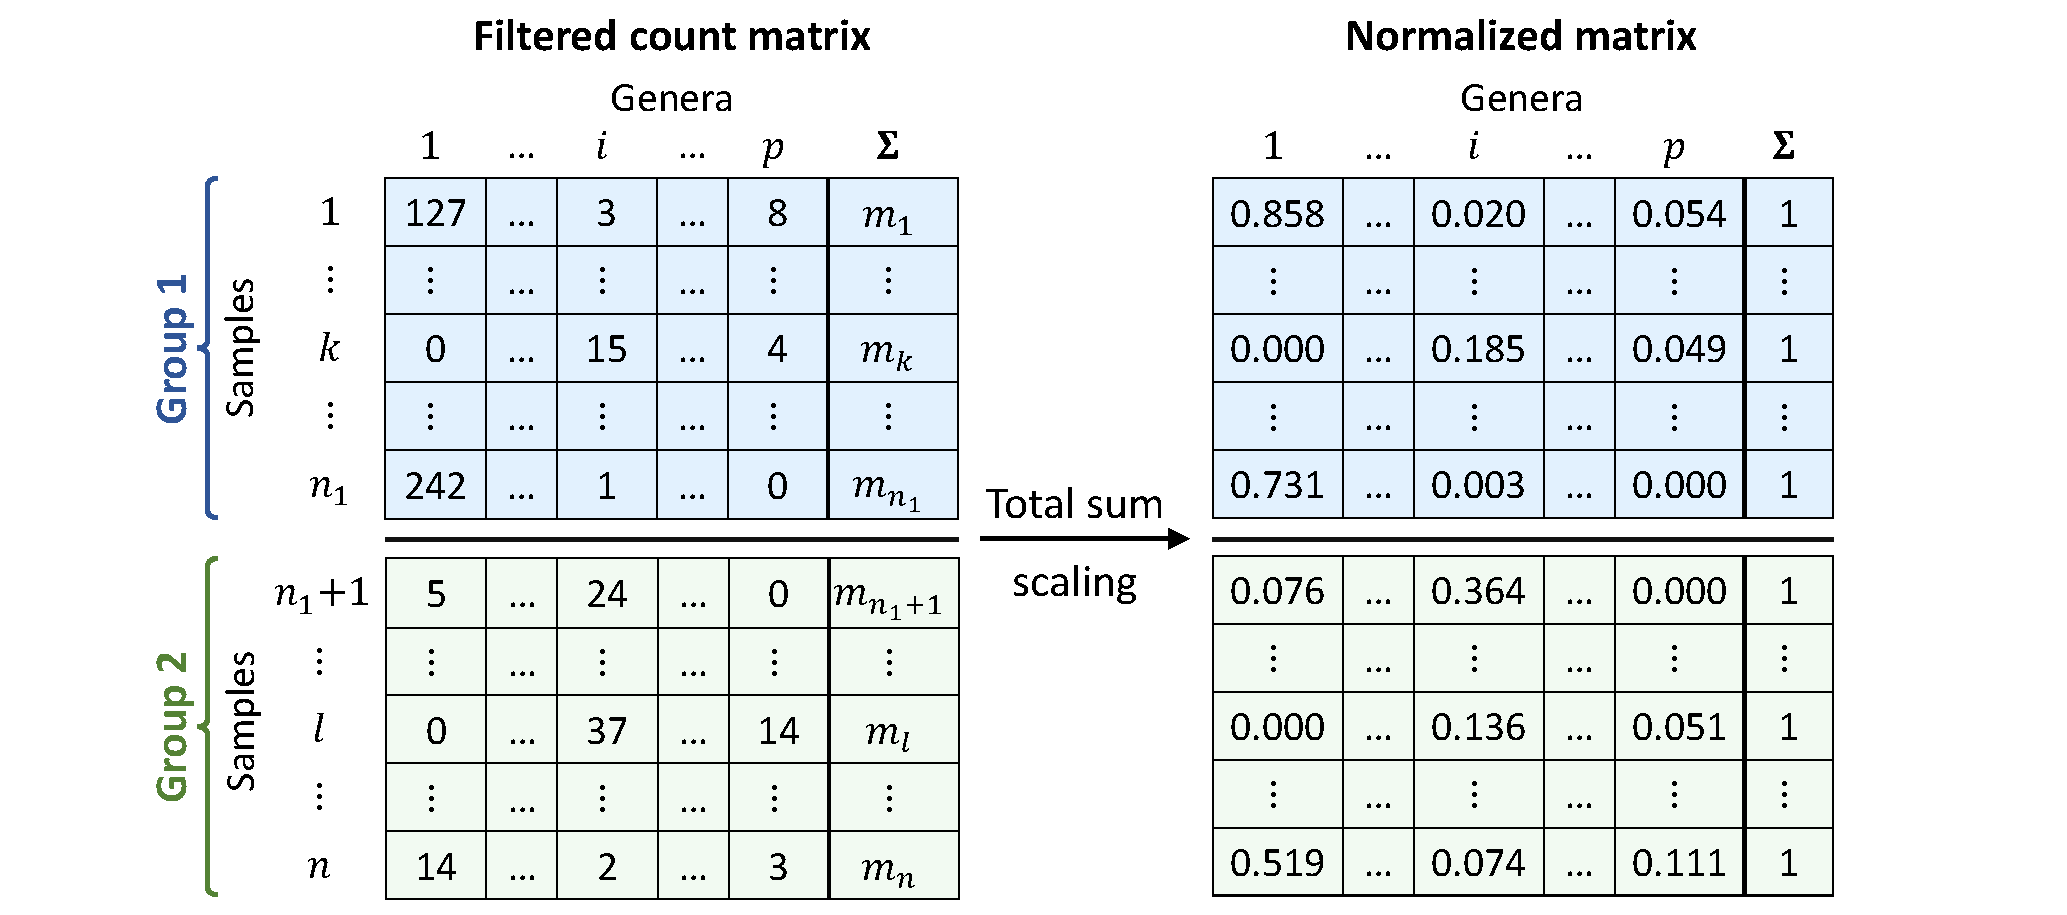
\includegraphics[width=\textwidth]{../ch02_microbiome_data/overview_figures/overview_normalization.pdf}
\caption{\textbf{Overview of normalization by total sum scaling.} The figure illustrates library-size adjustment of a filtered genus-level count matrix by total sum scaling. For each sample, counts are divided by the corresponding library size, shown in the column $\Sigma$ of the count matrix. The resulting normalized matrix contains relative abundances, here rounded to three decimal places, and each row sums to one before rounding. The two colored sample blocks represent two groups and are shown for consistency with later comparative analyses. The normalization step itself is applied sample-wise and is not group-specific.}
\label{fig:2micro:overview_normalization}
\end{figure}

After filtering and taxonomic aggregation, microbiome count matrices still contain samples with heterogeneous library sizes. Since the total number of reads differs between samples, raw counts are not directly comparable across samples: a taxon with the same relative contribution to two microbial communities will, on average, yield more reads in the sample with larger library size. Normalization aims to reduce artifactual variation induced by uneven sequencing depth, thereby making measurements from different samples more comparable \citep{weiss2017normalization}. It does not, however, generally remove other sources of technical variation, such as batch effects or taxon-specific amplification bias. In the narrower sense used in this chapter, normalization refers to preprocessing steps that adjust for heterogeneous library sizes or bring samples to a common compositional scale, without changing the coordinate system in which the data are represented.

Figure~\ref{fig:2micro:overview_normalization} illustrates this idea for total sum scaling, the normalization step used in the CLR-based analyses of this thesis. Starting from the filtered genus-level count matrix, each row is divided by its corresponding library size. The resulting normalized matrix contains relative abundances, and each sample sums to one. Thus, total sum scaling removes differences in the total count scale while preserving the within-sample ratios among non-zero counts.


This distinction between normalization and transformation is important because both terms are sometimes used interchangeably in the microbiome literature. In this thesis, transformations are treated separately in Section~\ref{sec:2micro:transformation}: they map the data into a new representation, for example by stabilizing variance or by expressing compositions in log-ratio coordinates. Normalization, by contrast, acts before such transformations and addresses the fact that samples may have been sequenced to different depths.

The ordering of preprocessing steps matters in particular for analyses based on log-ratio transformations. Since log-ratio transformations require strictly positive components, zero replacement is needed before applying them. However, if replacement values are defined on the raw count scale, the same numerical replacement value has different relative weight in samples with different library sizes. For this reason, the CLR-based analyses in this thesis first bring samples to a common compositional scale by total sum scaling, then perform zero replacement, and finally apply the CLR transformation. The present section introduces normalization methods for library-size adjustment, while zero handling and transformations are discussed in the following sections.

%====================================
\subsection{Scaling-based library size adjustment}
\label{sec:2micro:norm:scaling}
%====================================

A common strategy for addressing heterogeneous library sizes consists of rescaling counts by sample-specific factors. 
In general form, scaling replaces the original counts $x_{ki}$ by
\begin{equation}
\tilde{x}_{ki} = \frac{x_{ki}}{s_k}, \qquad k=1,\dots,n,\;i=1,\dots,p,
\end{equation}
where $s_k>0$ is a sample-specific scaling factor. 
The choice of $s_k$ determines the normalization method.

%------------------------------------
\subsubsection*{Total sum scaling (TSS)}
%------------------------------------

The simplest scaling-based approach uses the observed library size $m_k=\sum_{i=1}^p x_{ki}$ as the sample-specific scaling factor. This leads to \emph{total sum scaling} (TSS), where each count is divided by the total number of reads in the corresponding sample:
\begin{equation}
\tilde{x}^{\mathrm{TSS}}_{ki} = \frac{x_{ki}}{m_k}.
\end{equation}
The resulting values are relative abundances and each normalized sample satisfies $\sum_{i=1}^p \tilde{x}^{\mathrm{TSS}}_{ki}=1$. TSS therefore places all samples on a common total-count scale and removes variation due solely to differences in the observed library size.

However, TSS does not remove the compositional dependence induced by closure. Moreover, it does not account for the fact that detection probabilities depend on sequencing depth. Rare taxa that are unobserved in shallow samples may appear at low but non-zero relative abundances in deeper samples, potentially distorting prevalence estimates and correlation patterns \citep{weiss2017normalization}. In addition, because all components are scaled by the total library size, a few highly abundant taxa can strongly influence the normalized values of all other taxa. Several alternative scaling procedures therefore replace the total library size $m_k$ by more robust estimates of the sample-specific scaling factor $s_k$, typically under structural assumptions about the majority of taxa being unchanged or about the influence of highly abundant features.

%------------------------------------
\subsubsection*{Cumulative sum scaling (CSS)}
%------------------------------------

Cumulative sum scaling (CSS) replaces the total library size $m_k$ by a partial sum of the count distribution. More precisely, the scaling factor $s_k$ is defined as the cumulative sum of counts up to a data-driven percentile, excluding the largest counts from the normalization factor \citep{paulson2013differential,badri2020shrinkage}. The motivation is that highly abundant taxa can dominate the total library size and thereby influence the normalized values of all remaining taxa. By using only a lower part of the count distribution, CSS aims to reduce this sensitivity while still adjusting for differences in sequencing depth.

%------------------------------------
\subsubsection*{Common sum scaling (COM)}
%------------------------------------

Common sum scaling (COM) rescales all samples to a common library size, usually chosen as the smallest observed library size $m_{\min}=\min_k m_k$. In the scaling formulation, this corresponds to using
\begin{equation}
s_k = \frac{m_k}{m_{\min}},
\end{equation}
so that the rescaled counts satisfy $\sum_{i=1}^p \tilde{x}_{ki}=m_{\min}$ for each sample $k$ \citep{badri2020shrinkage}. Unlike rarefaction (cf. Section~\ref{sec:2micro:norm:rarefaction}), which also aims to equalize library sizes, COM achieves this by deterministic rescaling rather than by random subsampling.

%------------------------------------
\subsubsection*{Relative log expression (RLE)}
%------------------------------------

Size-factor methods originally developed for RNA-seq data have also been adapted to microbiome count data. These approaches estimate $s_k$ under the assumption that most features do not exhibit systematic changes across the samples or conditions under study, so that a typical multiplicative difference can be interpreted as a technical size factor rather than as a global biological shift. The relative log expression (RLE) method implemented in the \texttt{DESeq2} \textsf{R} package \citep{love2014moderated} computes, for each sample, the median ratio of counts to a pseudo-reference sample defined by the geometric mean across samples \citep{badri2020shrinkage}. The resulting size factor represents the typical multiplicative deviation of that sample from the reference.

%------------------------------------
\subsubsection*{Trimmed mean of M-values (TMM)}
%------------------------------------

The trimmed mean of M-values (TMM) normalization implemented in \texttt{edgeR} \citep{robinson2010edger,chen2025edger} estimates scaling factors based on log fold changes relative to a reference sample. To reduce the influence of extreme observations, the calculation trims features with very large log fold changes or expression levels before computing the normalization factor. This makes TMM less sensitive to highly abundant or strongly differential features than simple total-sum based scaling \citep{baruzzo2022beware}.

%------------------------------------
\subsubsection*{Geometric mean of pairwise ratios (GMPR)}
%------------------------------------

The geometric mean of pairwise ratios (GMPR) method was proposed specifically for sparse sequencing data with many zero counts \citep{chen2018gmpr}. Instead of relying on a pseudo-reference based on feature-wise geometric means, which can be problematic when many features contain zeros, GMPR estimates sample-specific size factors from median pairwise ratios between samples. This construction makes the method more robust in sparse microbiome count matrices, where many taxa are absent or unobserved in a large fraction of samples. 

The assumptions underlying the RLE and TMM approaches were originally developed for gene-expression data and may be difficult to justify in microbiome studies when a substantial proportion of taxa changes jointly between groups or when compositional effects dominate the observed counts.

%====================================
\subsection{Rarefaction}
\label{sec:2micro:norm:rarefaction}
%====================================

The scaling-based methods discussed above adjust for heterogeneous library sizes by multiplying all counts in a sample by a sample-specific factor. Rarefaction follows a different principle. Instead of rescaling the observed counts, it equalizes library sizes by randomly subsampling reads from each sample to a common target depth $m_{\mathrm{rare}}$, usually without replacement \citep{mcmurdie2014waste}. The target depth is often chosen as the smallest observed library size $m_{\min}=\min_k m_k$ or as a larger quantile of the library-size distribution. In the latter case, samples with library sizes below the chosen target must be excluded from the rarefied data set. Conditional on the observed count vector $\mathbf{x}_k=(x_{k1},\ldots,x_{kp})^\top$, the rarefied count vector can be viewed as a random draw from the observed reads and satisfies
\begin{equation}
\sum_{i=1}^p \tilde{x}^{\mathrm{rare}}_{ki} = m_{\mathrm{rare}}.
\end{equation}
More explicitly, this subsampling step can be described by a multivariate hypergeometric distribution,
\begin{equation}
\tilde{\mathbf{x}}^{\mathrm{rare}}_k \sim \operatorname{MultivariateHypergeometric}\left(m_{\mathrm{rare}},x_{k1},\ldots,x_{kp}\right).
\end{equation}

Rarefaction directly enforces equal library sizes and is therefore particularly intuitive for analyses based on ecological dissimilarities or observed diversity measures, where unequal sampling effort can otherwise dominate comparisons between samples. At the same time, rarefaction modifies the observed count matrix in a fundamentally different way than deterministic rescaling: it discards reads from samples with library size larger than $m_{\mathrm{rare}}$, introduces additional sampling variability, and may turn originally non-zero low counts into zeros.

For this reason, rarefaction has been one of the most controversial preprocessing steps in microbiome data analysis. \citet{mcmurdie2014waste} argued that rarefying is statistically inadmissible because it discards observed counts, reduces power, and performs unfavorably compared with model-based approaches in differential abundance settings. In contrast, \citet{schloss2023waste} revisited this conclusion and argued that the original comparison was affected by simulation and analysis choices that made rarefaction appear worse than it is. More recently, \citet{schloss2026rarefaction} further argued, based on simulations and re-analyses of case studies, that rarefaction can control uneven sequencing effort more effectively than robust Aitchison PCA and several other compositional or normalization-based approaches in distance-based analyses of amplicon data.

These apparently conflicting conclusions are less contradictory when the downstream analysis target is made explicit. Rarefaction is mainly relevant when the objective is to compare community-level summaries, such as alpha diversity, beta diversity, ordination, or PERMANOVA-type analyses, under heterogeneous library sizes. In such settings, equalizing the number of reads can reduce the extent to which distances or diversity estimates reflect sampling effort rather than biological variation. For feature-level differential abundance testing or association network estimation, however, rarefaction is generally not a universal solution. Several differential abundance methods model raw counts and incorporate their own adjustment for library size or sampling depth, while compositionally-aware network methods often rely on log-ratio, proportionality, or sparse graphical-model approaches. Rarefying before such methods may unnecessarily increase sparsity and remove information that the model is designed to use. Thus, rarefaction should not be understood as a generally optimal normalization strategy, but as a context-dependent tool whose usefulness depends on the inferential target and the assumptions of the downstream method.

%%%%%%%%%%%%%%%%%%%%%%%%%%%%%%%%%%%%%
\section{Handling zero counts}
\label{sec:2micro:zeros}
%%%%%%%%%%%%%%%%%%%%%%%%%%%%%%%%%%%%%

\begin{figure}[H]
\centering
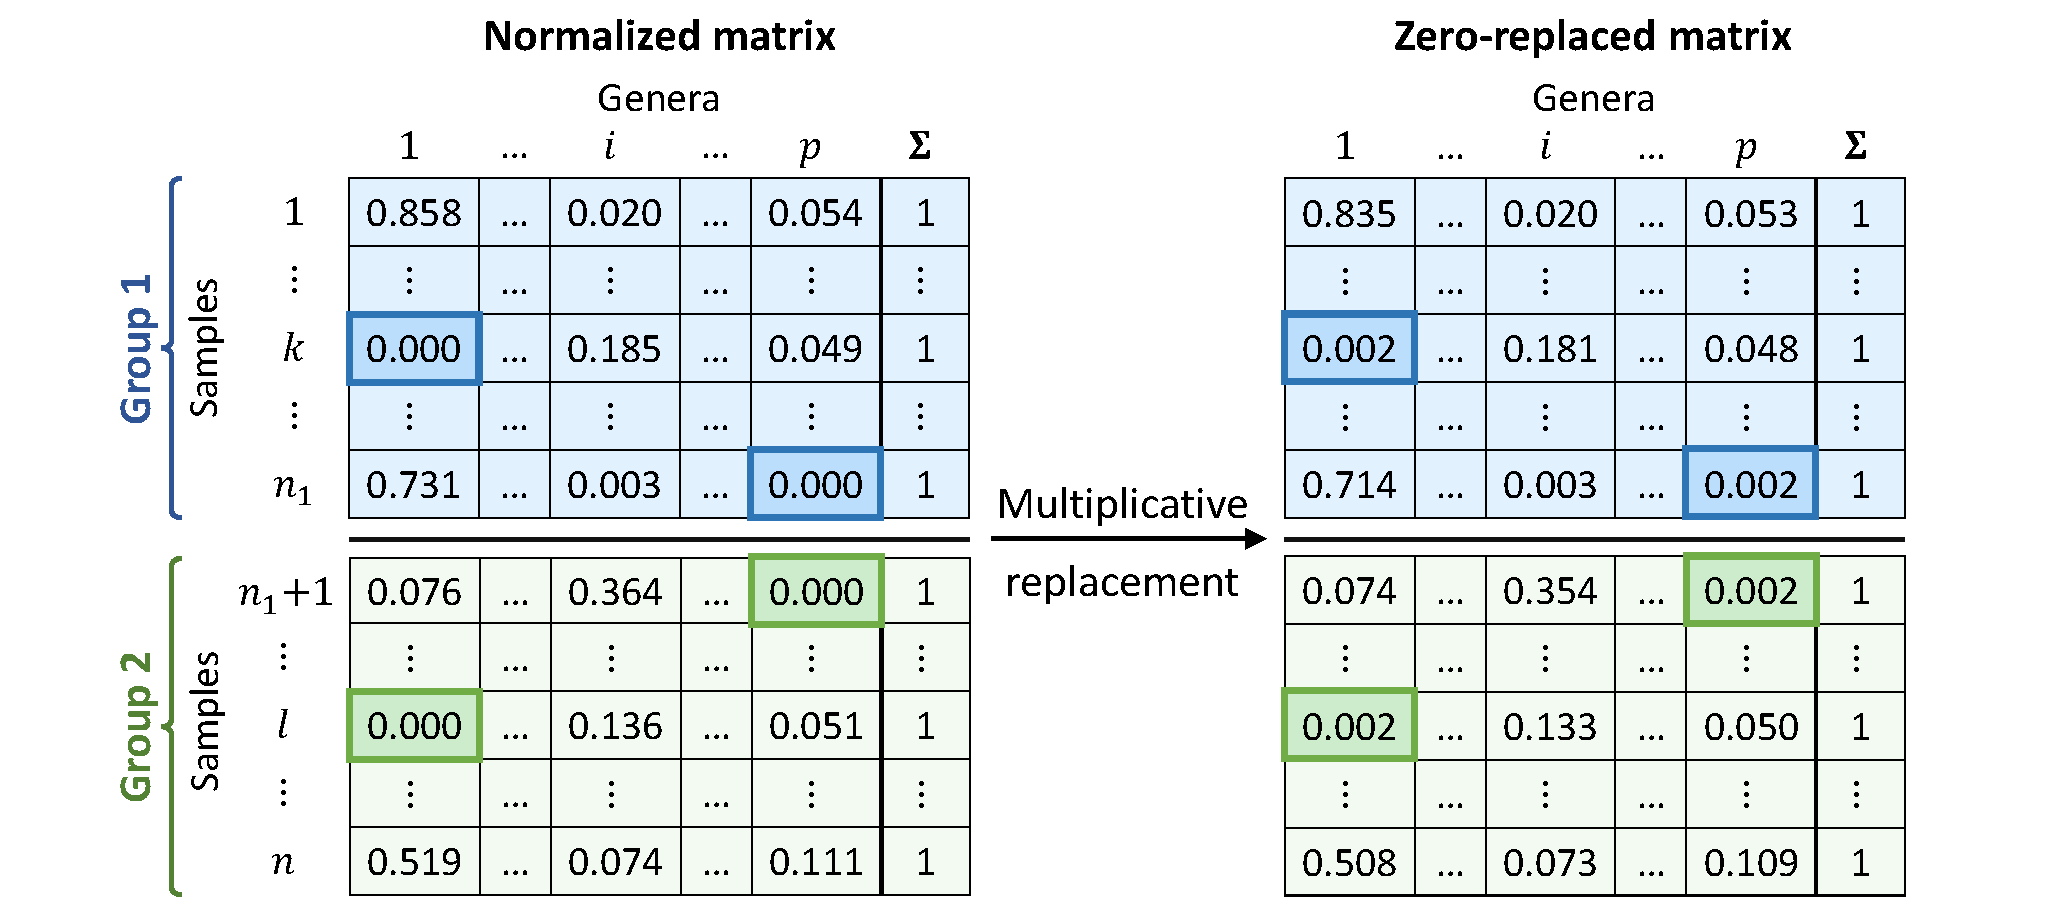
\includegraphics[width=\textwidth]{../ch02_microbiome_data/overview_figures/overview_zero_replacement.pdf}
\caption{\textbf{Overview of zero replacement by multiplicative replacement.} The figure illustrates zero replacement for a normalized genus-level matrix after total sum scaling. Zero entries are replaced by a small positive value $\delta$, while the non-zero entries in the same sample are adjusted multiplicatively so that the sample remains on the same compositional scale. In the example shown, the detection limit $DL$ is defined as the minimum non-zero matrix entry, and the replacement value is chosen as $\delta = 0.65 \cdot DL$, corresponding to the default setting in \texttt{multRepl()}. Matrix entries are rounded to three decimal places, so that the replacement value appears as $0.002$. The two colored sample blocks represent two groups and are shown for consistency with later comparative analyses. The zero-replacement step itself is applied sample-wise and is not group-specific.}
\label{fig:2micro:overview_zeros}
\end{figure}

Even after filtering and library-size adjustment, microbiome data usually remain sparse and contain many zero entries. These zeros are not merely inconvenient numerical values, but may reflect biological absence, limited sequencing depth, detection limits, or other technical aspects of the measurement process. Their interpretation is therefore ambiguous: the same observed value $x_{ki}=0$ may indicate that taxon $i$ is truly absent from sample $k$, or that it was present but not observed by the sequencing process.

This ambiguity matters because many statistical models interpret a zero count according to an implicit data-generating mechanism, for example as an observed count outcome or as evidence of absence. For count-based models, this may affect assumptions about the data-generating process and dispersion structure. For compositional methods, the problem is even more direct: log-ratio transformations require strictly positive components and are therefore undefined in the presence of zeros. Zero handling is thus not only a computational prerequisite for some methods, but also a modeling decision about how unobserved or undetected taxa should enter the analysis.

\newpage
In the preprocessing order used in this thesis for CLR-based analyses (cf. Section~\ref{sec:2micro:preprocessing_choices_thesis}), zero replacement is applied after bringing samples to a common compositional scale by total sum scaling. This order is important because replacement values defined on the raw count scale would have different relative weight in samples with different library sizes. Applying zero replacement on the relative abundance scale instead makes the imputed values comparable across samples in compositional terms. At the same time, the general principles discussed below apply more broadly to compositional vectors with arbitrary constant sum. Figure~\ref{fig:2micro:overview_zeros} illustrates this step for multiplicative replacement, which is the default zero-handling approach used later for CLR-based analyses.

In the following, we first distinguish the main types of zeros discussed in compositional data analysis and microbiome methodology. We then summarize common replacement and imputation strategies and discuss their implications for downstream analyses.

%====================================
\subsection{Types of zeros}
\label{sec:2micro:zeros:types}
%====================================

Several classifications of zeros have been proposed in the compositional data analysis (CoDA) literature and in microbiome methodology.

A common distinction proposed by \citet{martin2011dealing} differentiates between:

\begin{itemize}
    \item \textbf{Essential / structural zeros:} The taxon is assumed to be truly absent from the sample. Under this interpretation, replacing the zero by a small positive value would be inappropriate.
    
    \item \textbf{Rounded zeros:} The taxon is present but its abundance lies below a detection limit or is rounded to zero due to measurement precision.

    \item \textbf{Count / sampling zeros:} The taxon is present in the environment but not observed due to limited sequencing depth.
\end{itemize}

For next-generation sequencing data, \citet{quinn2019field} emphasize that many observed zeros may arise through finite sampling, since increasing sequencing depth can reveal additional low-abundance taxa.
Similarly, \citet{paulson2013differential} report a strong association between sequencing depth and the number of detected taxa, which is consistent with at least some zeros reflecting undersampling rather than true absence.

\citet{kaul2017analysis} introduce an alternative classification distinguishing structural zeros, sampling zeros, and \emph{outlier zeros}, where the latter arise from extraneous technical effects rather than detection limits. 

Importantly, the nature of a zero is typically not identifiable from the observed count matrix alone. The classification therefore depends on substantive knowledge and modeling assumptions.

%====================================
\subsection{Replacement and imputation strategies}
\label{sec:2micro:zeros:replacement}
%====================================

Because log-ratio transformations require strictly positive values, zero handling often involves either replacing zeros by small positive values or imputing them using a statistical model. 
These approaches differ in how strongly they perturb the relative structure of the data and in the extent to which they preserve compositional properties such as scale invariance and subcompositional coherence. In the following, it is useful to distinguish between strategies that add an offset to all components, strategies that replace only zero components, and imputation methods that use multivariate structure across samples and taxa.

\noindent\textbf{Global offset addition.}
A simple strategy often used in microbiome analysis is to add a constant, for example $1$, to all counts before applying a logarithmic transformation \citep{mcmurdie2013phyloseq,weiss2017normalization}. This strategy is computationally convenient because it makes all components positive. However, it modifies all components, including those that were originally non-zero. Consequently, ratios among observed components are changed. For example, for two positive components $x_i>0$ and $x_j>0$, adding a constant $\delta>0$ changes the ratio from
$x_i/x_j$ to $(x_i+\delta)/(x_j+\delta)$.
These two ratios are generally not equal. Thus, global offset addition does not only resolve zeros, but also perturbs relative information among taxa that were observed. As illustrated in Table~\ref{tab:zero_replacement}, this alters ratios among originally non-zero components and therefore changes the relative structure of any subcomposition containing them.

\noindent\textbf{Zero-only replacement.}
A simple strategy is to replace only entries equal to zero by a small positive value while leaving the non-zero components unchanged. This preserves ratios among originally non-zero components, because the positive entries themselves are not altered relative to one another. However, if the data are treated as compositions, the components are constrained to a fixed total, either on the count scale or after closure to unit sum. The positive mass assigned to zeros must therefore be accounted for. Without an appropriate adjustment of the positive components, the total sum of the modified composition increases, and the resulting vector no longer lies in the same simplex as the original composition. Thus, zero-only replacement is useful for illustrating the principle of preserving observed ratios, but a coherent replacement of a composition usually requires an additional rescaling step. Multiplicative replacement implements this idea by assigning small positive values to zeros and reducing the originally non-zero components proportionally.

\noindent\textbf{Multiplicative replacement.}
To preserve ratios among non-zero components while maintaining the compositional structure, \citet{martin-fernandez2003dealing} proposed multiplicative replacement. In contrast to global offset addition, multiplicative replacement does not add a constant to all components. Instead, zero components are replaced by small positive values and the originally non-zero components are adjusted proportionally so that the constant-sum constraint is preserved.
Although the notation below is written for a generic non-negative composition, in the default CLR-based pipeline of this thesis the vector entering multiplicative replacement is the relative abundance vector obtained after total sum scaling.

For sample $\mathbf{x}_k=(x_{k1},\ldots,x_{kp})^\top$ with sample total
\begin{equation}
C_k=\sum_{i=1}^p x_{ki},
\label{eq:2micro:sample_total_multiplicative_replacement}
\end{equation}
let $Z_k=\{i:x_{ki}=0\}$ denote the set of zero components. Following the formulation of \citet{martin-fernandez2003dealing}, the replacement can be written as
\begin{equation}
x_{ki}^\ast =
\begin{cases}
\delta_i, & x_{ki}=0,\\
\left(1-\frac{\sum_{j\in Z_k}\delta_j}{C_k}\right)x_{ki}, & x_{ki}>0,
\end{cases}
\label{eq:2micro:multiplicative_replacement_general}
\end{equation}
where $\delta_i>0$ is the imputed value for component $i$. The proportional factor applied to all non-zero components ensures that the sample total remains unchanged:
\begin{equation}
\sum_{i=1}^p x_{ki}^\ast = C_k.
\label{eq:2micro:multiplicative_replacement_total}
\end{equation}
This formulation allows component-specific replacement values, which is useful when detection limits differ between taxa or features.

For the replacement to be well defined, the total imputed mass must satisfy
\begin{equation}
	\sum_{j\in Z_k}\delta_j < C_k,
\end{equation}
so that the multiplicative adjustment factor for the originally non-zero components remains positive.

Since all originally non-zero components within sample $k$ are multiplied by the same factor, ratios among them are preserved. If $x_{ki}>0$ and $x_{kj}>0$, then
\begin{equation}
\frac{x_{ki}^\ast}{x_{kj}^\ast}
=
\frac{\left(1-\frac{\sum_{\ell\in Z_k}\delta_\ell}{C_k}\right)x_{ki}}
{\left(1-\frac{\sum_{\ell\in Z_k}\delta_\ell}{C_k}\right)x_{kj}}
=
\frac{x_{ki}}{x_{kj}}.
\label{eq:2micro:multiplicative_replacement_ratio}
\end{equation}
This ratio preservation is a key reason why multiplicative replacement is commonly used before log-ratio transformations. It differs from additive modifications of non-zero components, which can alter ratios among parts that were originally observed. Table~\ref{tab:zero_replacement} illustrates these differences for a simple three-part composition.

In practice, nonparametric multiplicative replacement for rounded or left-censored zeros is implemented, for example, in the function \texttt{multRepl()} of the \texttt{zCompositions} package \citep{palarea-albaladejo2015zcompositions}. This function requires a detection limit for each component and, by default, replaces a zero by a fraction of this limit. In sequencing data, however, detection limits are not always explicitly defined in the same way as in classical censored compositional data. Therefore, replacement values should be chosen in accordance with the scale and preprocessing context of the analysis.

\begin{table}[!htb]
\centering
\caption{Illustration of ratio preservation and subcompositional coherence for the composition $\mathbf{x}=(x_1,x_2,x_3)^\top$ with subcomposition $\operatorname{sub}(\mathbf{x})=(x_2,x_3)^\top$. The table compares global offset addition, zero-only replacement, and multiplicative replacement. The replacement value in each case is $\delta = 0.1$. Global offset addition changes the ratio $x_2/x_3$ and alters the relative structure of the subcomposition. In contrast, zero-only replacement and multiplicative replacement preserve the ratio among originally non-zero components. Multiplicative replacement additionally preserves the compositional total by proportionally adjusting the non-zero components.}
\label{tab:zero_replacement}
\small
\setlength{\tabcolsep}{8pt}
\renewcommand{\arraystretch}{1.15}
\begin{tabular}{l|ccc|cc|c}
\textbf{Method} & ${x_1}$ & ${x_2}$ & ${x_3}$ & ${\sum \mathbf{x}}$ & ${\sum \operatorname{sub}(\mathbf{x})}$ & ${x_2/x_3}$  \\
\hline\hline
\textbf{Original vector} & $0$ & $0.2$ & $0.8$ & $1$ & $1$ & $0.25$\\
\hline
\textbf{Global offset addition} & $0.1$ & $0.3$ & $0.9$ & $1.3$ & $1.2$ & $0.333$ \\
Renormalize $\mathbf{x}$ to sum $1$ & $0.077$ & $0.231$ & $0.692$ & $1$ & ~ & $0.333$ \\
Renormalize sub($\mathbf{x}$) to sum $1$ & ~ & $0.25$ & $0.75$ & ~ & $1$ & $0.333$ \\
\hline
\textbf{Zero-only replacement} & $0.1$ & $0.2$ & $0.8$ & $1.1$ & $1$ & $0.25$ \\
Renormalize $\mathbf{x}$ to sum $1$ & $0.091$ & $0.182$ & $0.727$ & $1$ & ~ & $0.25$  \\
Renormalize sub($\mathbf{x}$) to sum $1$ & ~ & $0.2$ & $0.8$ & ~ & $1$ & $0.25$ \\
\hline
\textbf{Multiplicative replacement} & $0.1$ & $0.18$ & $0.72$ & $1$ & $0.9$& $0.25$ \\
Renormalize sub($\mathbf{x}$) to sum $1$ & ~ & $0.2$ & $0.8$ & ~ & $1$ & $0.25$ \\
\end{tabular}
\end{table}

\noindent\textbf{Bayesian multiplicative replacement for count zeros.}
Bayesian multiplicative replacement was proposed for compositional count data, where zeros are interpreted as count zeros resulting from limited sampling rather than as confirmed structural absences \citep{martin-fernandez2015bayesianmultiplicative}. For each sample $k$, the count vector $\boldsymbol{x}_k=(x_{k1},\ldots,x_{kp})$ is modeled using a multinomial distribution with a Dirichlet prior on the underlying composition,
\begin{equation}
\boldsymbol{x}_k \mid \boldsymbol{\pi}_k
\sim
\operatorname{Multinomial}(C_k,\boldsymbol{\pi}_k),
\qquad
\boldsymbol{\pi}_k
\sim
\operatorname{Dirichlet}(\boldsymbol{\alpha}_k).
\label{eq:2micro:bayesian_multiplicative_model}
\end{equation}
The resulting posterior estimates provide strictly positive values for all components, including those observed as zeros, and yield a composition with the original sample total after rescaling.

In contrast to ordinary multiplicative replacement, the replacement values depend on the library size and on prior information about the expected composition. In the Bayesian multiplicative method implemented in \texttt{cmultRepl()} from \texttt{zCompositions}, prior information about the underlying composition is estimated from the observed data, with the precise construction depending on the selected method and settings \citep{martin-fernandez2015bayesianmultiplicative,palarea-albaladejo2015zcompositions}. Thus, replacement is carried out sample-wise while borrowing limited information from the remaining samples. This method is considered as a sensitivity analysis for CLR-based network construction in the application chapter.

\noindent\textbf{ALR-EM imputation for rounded zeros.}
The modified ALR-EM algorithm of \citet{palarea-albaladejo2008modified} takes a different perspective. It treats rounded zeros as values below a component-specific detection limit and therefore as censored rather than sampled zero observations. The method first maps compositions to additive log-ratio coordinates using a selected reference component. It then assumes a multivariate normal model in ALR space and iteratively estimates the model parameters and the censored values using a modified expectation-maximization algorithm. After convergence, the imputed ALR coordinates are mapped back to the simplex.

Unlike multiplicative replacement, ALR-EM explicitly borrows information across samples and components through the estimated covariance structure. This may be advantageous when zeros plausibly represent values below detection limits and when the multivariate model is adequate. However, the method requires the specification of detection limits and depends on the chosen ALR reference component. Its assumptions are therefore stronger than those of simple or Bayesian multiplicative replacement. Like Bayesian multiplicative replacement, ALR--EM is used as an alternative zero-handling strategy in the comparison of network-construction pipelines in Chapter~\ref{ch:application}.


\noindent\textbf{Low-rank log-ratio imputation.}
Simple replacement rules are local in the sense that they do not use the multivariate structure of the full data set when replacing zeros. This can become problematic in highly sparse high-dimensional count data. A recent comparison by \citet{tang2026critical} discusses this limitation and reports that multiplicative replacement can perform well when the zero proportion is moderate, whereas multivariate imputation methods may be advantageous in highly sparse settings. One such method is log-ratio singular value decomposition (lrSVD), proposed by \citet{palarea-albaladejo2022lrsvd} for imputing missing and zero values in compositional data. The idea is to exploit low-rank structure in log-ratio space. After an initial replacement step, the data are transformed to log-ratio coordinates and approximated by a low-rank matrix. In simplified form, the complete-data problem can be expressed as
\begin{equation}
\min_R \|X-R\|_F^2
\qquad
\text{subject to}
\qquad
\operatorname{rank}(R)\leq s,
\label{eq:2micro:lrsvd_complete}
\end{equation}
where $s$ denotes the target rank and $\|\cdot\|_F$ is the Frobenius norm. For incomplete or censored data, lrSVD solves a constrained optimization problem in which the imputed values are required to remain within lower and upper bounds. In the case of rounded zeros, these bounds are determined by the detection limit. Thus, lrSVD differs fundamentally from simple replacement methods: it borrows information across samples and taxa and can therefore be more effective under high sparsity. However, this comes at the cost of additional assumptions, including an underlying low-rank structure, the choice of the target rank, and greater computational complexity.

\noindent\textbf{Further multivariate imputation methods.}
Beyond the methods introduced above, several approaches have been proposed that use multivariate information for zero imputation, for instance methods based on k-nearest neighbors, partial least squares regression, or other model-based formulations in log-ratio space \citep{hron2010imputation,templ2016imputation,lubbe2021comparison}. By borrowing information across samples and taxa, such methods may be useful in highly sparse data sets, but they require additional modeling assumptions and tuning choices. Implementations of a range of zero-replacement and imputation methods are available in the \texttt{zCompositions} \citep{palarea-albaladejo2015zcompositions} and \texttt{robCompositions} \citep{templ2011robcompositions} packages.

%%%%%%%%%%%%%%%%%%%%%%%%%%%%%%%%%%%%%
\section{Transformations}
\label{sec:2micro:transformation}
%%%%%%%%%%%%%%%%%%%%%%%%%%%%%%%%%%%%%

\begin{figure}[H]
\centering
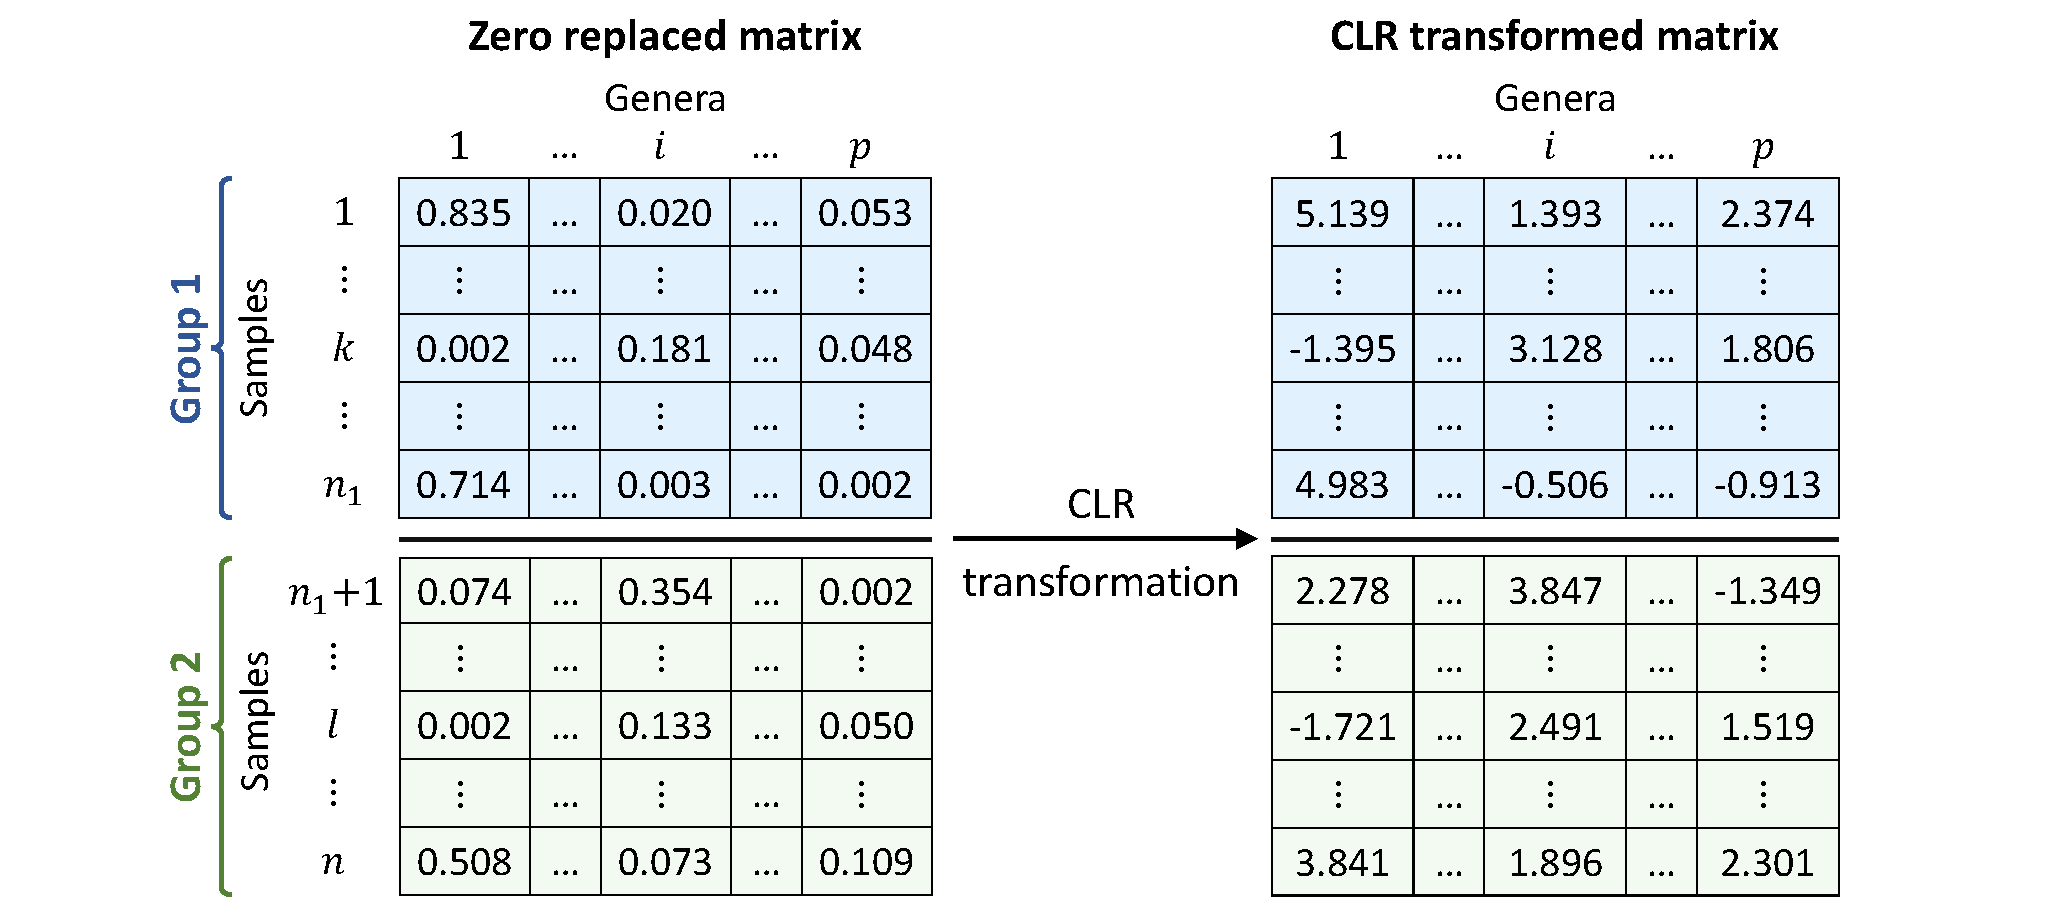
\includegraphics[width=\textwidth]{../ch02_microbiome_data/overview_figures/overview_transformation.pdf}
\caption{\textbf{Overview of transformation by the centered log-ratio (CLR).} The figure illustrates the transformation of a zero-replaced genus-level matrix to CLR coordinates. For each sample, the strictly positive entries are transformed by taking logarithms relative to the sample-wise geometric mean. The resulting CLR-transformed matrix contains real-valued log-ratio coordinates, which may be positive or negative and are no longer constrained to sum to one. Matrix entries are shown rounded to three decimal places. The two colored sample blocks represent two groups and are shown for consistency with later comparative analyses. The transformation itself is applied sample-wise and is not group-specific.}
\label{fig:2micro:overview_transformation}
\end{figure}

After filtering, library-size adjustment, and zero handling where needed, microbiome data may still require a representation that is better suited to the statistical analysis of interest. Transformations map the data into a new coordinate system or numerical scale. They may be used to stabilize the mean--variance relationship of count data, to reduce skewness, or to represent compositional observations in log-ratio coordinates. In contrast to normalization, transformations do not primarily aim to make library sizes comparable, but define the variables on which downstream models, distances, and test statistics are computed.

This distinction is important because the terms \emph{normalization} and \emph{transformation} are sometimes used interchangeably in the microbiome literature. As discussed in Section~\ref{sec:2micro:normalization}, normalization aims to reduce artifactual variation and to make measurements more comparable across samples \citep{weiss2017normalization}. Transformations, in contrast, map the data into a new space, often a Euclidean space, to facilitate statistical modeling but do not recover absolute abundance information from relative measurements \citep{quinn2019field}. As emphasized by \citet{quinn2019field}, transformations are not normalizations: transformed values must always be interpreted relative to the chosen reference or coordinate system.

In microbiome data analysis, two transformation goals are particularly relevant. First, transformations such as variance-stabilizing transformations aim to reduce the dependence between the mean and variance of count data, which can improve the behavior of methods that assume approximately homoscedastic observations. Second, log-ratio transformations address the compositional structure of sequencing data by representing samples through ratios between components rather than through raw counts or proportions. Figure~\ref{fig:2micro:overview_transformation} illustrates this second perspective for the centered log-ratio (CLR) transformation, which is the default transformation used in the CLR-based analyses of this thesis. These two perspectives are not mutually exclusive, but they target different statistical problems and lead to different interpretations of the transformed values.

%====================================
\subsection{Variance-stabilizing transformations}
\label{sec:2micro:norm:vst}
%====================================

Beyond library size adjustment, transformations have been proposed that aim to stabilize the variance of count data in the presence of overdispersion. 
Such methods primarily address goal (2), namely the dependence of the variance on the mean.

For sequencing counts, the variance typically increases with the expected value. 
Under a Poisson model, $\mathrm{Var}(X)=\mathbb{E}(X)$, while under negative binomial models commonly used for high-throughput sequencing data, the variance satisfies
\begin{equation}
\mathrm{Var}(X) = \mu + \alpha \mu^2,
\end{equation}
where $\mu$ denotes the mean and $\alpha>0$ is a dispersion parameter \citep{anders2010differential,robinson2010edger}. 
This mean–variance relationship induces heteroscedasticity that can distort distance-based analyses, clustering, and linear modeling.

Variance-stabilizing transformations seek a function $h(\cdot)$ such that
\begin{equation}
\mathrm{Var}\!\big(h(X)\big)
\approx \text{constant}.
\end{equation}

Within the \texttt{DESeq2} framework, a variance-stabilizing transformation is obtained by estimating the mean--dispersion relationship and applying a transformation of the general form \citep{love2014moderated}
\begin{equation}
\mathrm{VST}(x_{ki}) = \int^{x_{ki}} \frac{d\mu}{\sqrt{v(\mu)}},
\end{equation}
where $v(\mu)$ denotes the estimated mean–variance function. 
In practice, $v(\mu)$ is estimated from the data, and the transformation is applied to size-factor–normalized counts.

The VST transformation yields approximately homoscedastic values that can improve the behavior of clustering, ordination, and other exploratory analyses based on Euclidean geometry.
Unlike log-ratio transformations, however, VST does not explicitly account for the compositional constraint induced by closure.

In a systematic comparison of normalization and transformation methods for microbiome data, \citet{badri2020shrinkage} showed that correlation structures obtained after applying VST were similar to those obtained using the CLR transformation. 
In particular, \citet{badri2020shrinkage} found that Pearson correlation estimates obtained after VST were similar to those obtained after CLR transformation in the settings considered.
Thus, although VST is motivated by variance stabilization rather than compositional geometry, it may yield correlation patterns similar to CLR-based analyses in some settings.

%====================================
\subsection{Log-ratio transformations}
\label{sec:2micro:norm:log-ratios}
%====================================

A principled approach to the statistical analysis of compositional data was developed by \citet{aitchison1982statistical}, who argued that inference should be based on ratios between components rather than on the raw parts themselves. 
Because closure induces a constant-sum constraint, the components of a composition are inherently dependent (Section~\ref{sec:2micro:charact:compositionality}). 
Standard summaries such as means, variances, correlations, and regression coefficients computed directly on proportions are therefore generally subcompositionally incoherent \citep{aitchison1982statistical,aitchison1986statistical}. 

For each sample $k$, let
$\mathbf{x}_k = (x_{k1}, \dots, x_{kp})^\top$
denote its composition after closure to a constant sum. 
Forming ratios between two components removes the influence of the total sum. 
For taxa $i$ and $j$ in sample $k$, the ratio is given by
\begin{equation}
\frac{x_{ki}}{x_{kj}}.
\end{equation}
This ratio is invariant under multiplication of the entire composition by a positive constant and remains unchanged under closure. 
Ratios therefore isolate the relative information contained in the data and are invariant under scaling. Moreover, the ratio between two retained components is unchanged when additional components are removed from the composition  \citep{aitchison1982statistical,greenacre2021compositional}.

Ratios operate on a multiplicative scale. 
Taking logarithms converts multiplicative relationships into additive ones and yields Euclidean coordinate representations of the simplex in which conventional multivariate methods can be formulated \citep{aitchison1986statistical,greenacre2021compositional}. 

However, all log-ratio transformations require strictly positive components. Their application to sparse microbiome count data therefore requires either a prior zero-handling step or a transformation specifically designed for zero-containing data, as discussed in Section~\ref{sec:2micro:clr_with_zeros}.

Within Aitchison's framework and subsequent developments, several log-ratio transformations have been proposed. The most commonly used are the following.

%------------------------------------
\subsubsection*{Additive log-ratio transformation (ALR).}
%------------------------------------

The additive log-ratio (ALR) transformation expresses each component relative to a chosen reference taxon, say taxon $p$. 
For sample $k$, it is defined as
\begin{equation}
\label{eq:2micro:ALR}
\text{ALR}(\mathbf{x}_k)_i = \log \frac{x_{ki}}{x_{kp}},
\qquad i = 1,\dots,p-1.
\end{equation}

The ALR transformation yields a full-rank $(p-1)$-dimensional representation in $\mathbb{R}^{p-1}$ and is computationally straightforward. 
Because the transformed variables are unconstrained, standard regression and multivariate models can be formulated directly in ALR form \citep{aitchison1982statistical,aitchison1986statistical}. 

However, ALR depends on the choice of reference component and is therefore not permutation invariant. Moreover, Euclidean distances computed after ALR transformation do not generally coincide with Aitchison distances in the simplex \citep{aitchison1986statistical}. In microbiome applications, selecting such a reference can be difficult because a taxon should ideally be prevalent, stably measured, and scientifically interpretable across all samples.

%------------------------------------
\subsubsection*{Centered log-ratio transformation (CLR).}
%------------------------------------

To avoid the asymmetry induced by selecting a single reference, Aitchison proposed the centered log-ratio (CLR) transformation \citep{aitchison1986statistical}. 
For sample $k$, it is defined as
\begin{equation}
\label{eq:2micro:CLR}
\text{CLR}(\mathbf{x}_k)_i = \log \frac{x_{ki}}{g(\mathbf{x}_k)},
\qquad i = 1,\dots,p,
\end{equation}
where the geometric mean is
\begin{equation}
\label{eq:2micro:geometric_mean}
g(\mathbf{x}_k) = \left( \prod_{i=1}^{p} x_{ki} \right)^{1/p}.
\end{equation}

The geometric mean treats all taxa symmetrically, so that each CLR coordinate represents a component relative to the geometric mean of all components in the sample.
The CLR transformation satisfies
\begin{equation}
\sum_{i=1}^{p} \text{CLR}(\mathbf{x}_k)_i = 0,
\end{equation}
so that CLR-transformed data lie in a $(p-1)$-dimensional subspace of $\mathbb{R}^{p}$. 
Consequently, the CLR covariance matrix is singular. 
Nevertheless, the Aitchison distance between two compositions equals the Euclidean distance between their CLR-transformed representations \citep{aitchison1986statistical}. 

%------------------------------------
\subsubsection*{Isometric log-ratio transformation (ILR).}
%------------------------------------

The isometric log-ratio (ILR) transformation \citep{egozcue2003isometric} constructs $(p-1)$ orthonormal log-contrasts, typically defined through a sequential binary partition of the taxa. 
In general form, the $j$th ILR component for sample $k$ is
\begin{equation}
z_{kj} = \sqrt{\frac{r_j s_j}{r_j + s_j}}
\log\frac{\left( \prod_{i \in R_j} x_{ki} \right)^{1/r_j}}{
\left( \prod_{i \in S_j} x_{ki} \right)^{1/s_j}},
\qquad j = 1,\dots,p-1,
\end{equation}
where $R_j$ and $S_j$ partition the taxa into two non-overlapping groups of sizes $r_j$ and $s_j$ \citep{greenacre2021compositional}. 

The ILR transformation produces orthonormal log-contrasts with respect to the Aitchison geometry. 
In contrast to CLR, the resulting covariance matrix is nonsingular, and Euclidean distances in ILR space exactly equal Aitchison distances between compositions \citep{egozcue2003isometric,greenacre2021compositional}. 

%------------------------------------
\subsubsection*{Practical considerations.}
%------------------------------------

The choice between ALR, CLR (and its variants), and ILR depends on the inferential objective:
\begin{itemize}
    \item ALR may be appropriate when a scientifically meaningful and stable reference taxon exists,
    \item CLR provides a symmetric representation and is widely used in exploratory microbiome analyses and network inference,
    \item ILR provides an orthonormal and full-rank Euclidean representation of Aitchison geometry and is therefore useful when unconstrained covariance estimation or standard multivariate modeling is required. However, interpretation depends on the chosen orthonormal basis, which can complicate applied interpretation \citep{egozcue2003isometric,greenacre2021compositional}.
\end{itemize}

Importantly, none of these transformations recover absolute abundances. All inference remains relative: differences between samples or groups must be interpreted with respect to ratios between taxa, or to a taxon relative to the chosen log-ratio reference, rather than as changes in absolute abundance \citep{quinn2019field}.

%%%%%%%%%%%%%%%%%%%%%%%%%%%%%%%%%%%%%
s\section{CLR transformations in the presence of zeros}
\label{sec:2micro:clr_with_zeros}
%%%%%%%%%%%%%%%%%%%%%%%%%%%%%%%%%%%%%

The preceding sections considered zero handling and log-ratio transformations as separate preprocessing problems. In practice, however, these two issues are tightly coupled. The CLR transformation is attractive for microbiome data because it represents each component relative to the geometric mean of the full composition and maps compositional data to a Euclidean space. At the same time, it requires strictly positive values and is therefore not directly applicable to sparse microbiome count matrices. Consequently, any CLR-based analysis of sequencing data requires a decision about how zeros are handled before or during transformation.

This section focuses on CLR-based representations because they play a central role in the analyses performed later in this thesis. In the application chapter, the CLR transformation is used whenever an analysis method allows the transformation to be chosen freely. This does not imply that CLR is universally preferable or that zero handling has a unique optimal solution. Rather, the aim is to make the consequences of this choice explicit and to compare different ways of combining zero handling with CLR-type transformations.

The following subsections therefore investigate several approaches, including global offset addition, multiplicative replacement before CLR transformation, and modified CLR variants that avoid replacing zeros directly. For each approach, we discuss the underlying idea, its advantages, and its limitations. This comparison provides the basis for the preprocessing choices used in the later chapters and clarifies which statistical interpretation is attached to the transformed microbiome data.

%====================================
\subsection{CLR after multiplicative replacement} 
\label{sec:2micro:clr_with_zeros:multRepl}
%====================================

A common way to make the CLR transformation applicable to sparse microbiome data is to first replace zeros by small positive values and subsequently apply the standard CLR transformation to the resulting strictly positive composition. Among the replacement strategies introduced in Section~\ref{sec:2micro:zeros:replacement}, multiplicative replacement is particularly compatible with the log-ratio interpretation of the CLR transformation, because it preserves ratios among originally non-zero components.

Let $\mathbf{x}_k^\ast$ denote the multiplicatively replaced version of sample $\mathbf{x}_k$. The CLR transformation is then given by
\begin{equation}
\operatorname{CLR}(\mathbf{x}_k^\ast)_i=\log\left(\frac{x_{ki}^\ast}{g(\mathbf{x}_k^\ast)}\right),
\label{eq:2micro:clr_after_mult_replacement}
\end{equation}
where $g(\mathbf{x}_k^\ast)$ denotes the geometric mean of the components of $\mathbf{x}_k^\ast$.

The relevance of multiplicative replacement becomes clear from the relationship between CLR coordinate differences and pairwise log-ratios. If $x_{ki}>0$ and $x_{kj}>0$, multiplicative replacement changes both components by the same sample-specific factor, so that
\begin{equation}
\frac{x_{ki}^\ast}{x_{kj}^\ast}=\frac{x_{ki}}{x_{kj}}.
\label{eq:2micro:mult_replacement_ratio_preservation}
\end{equation}
Since differences between CLR coordinates are pairwise log-ratios,
\begin{equation}
\operatorname{CLR}(\mathbf{x}_k^\ast)_i-\operatorname{CLR}(\mathbf{x}_k^\ast)_j
=
\log\left(\frac{x_{ki}^\ast}{x_{kj}^\ast}\right),
\label{eq:2micro:clr_difference_logratio}
\end{equation}
the observed log-ratios between non-zero components are retained after transformation. This property is important for analyses whose interpretation depends directly on log-ratio geometry, including Aitchison distances, proportionality, and CLR-based association measures.

At the same time, multiplicative replacement is still a replacement procedure and therefore introduces assumptions about the unobserved zero components. The magnitude of the replacement value influences the transformed values assigned to zeros and can affect distances or associations involving sparse taxa. Thus, multiplicative replacement followed by CLR should not be interpreted as recovering the unobserved true composition. Rather, it provides a zero-aware approximation to the standard CLR representation that preserves ratios among components that were actually observed.

%====================================
\subsection{Modified CLR (mCLR)} 
\label{sec:2micro:clr_with_zeros:mCLR}
%====================================

The modified centered log-ratio transformation (mCLR) was proposed in the context of sparse microbial graphical modeling, in particular for the SPRING framework of \citet{yoon2019microbial}. In contrast to replacement-based approaches, mCLR does not replace zero counts by positive values before transformation. Instead, it computes the geometric mean only over the positive components of each sample and leaves zero components unchanged.

For a sample $\mathbf{x}_k=(x_{k1},\ldots,x_{kp})^\top$, let $P_k=\{i:x_{ki}>0\}$ denote the index set of positive components, and let $\mathbf{x}_k^+=(x_{ki}:i\in P_k)^\top$ denote the corresponding positive subvector. The ordinary geometric mean of the positive components is
\begin{equation}
g(\mathbf{x}_k^+)=\left(\prod_{i\in P_k}x_{ki}\right)^{1/|P_k|}.
\label{eq:2micro:positive_geometric_mean}
\end{equation}
The mCLR transformation is defined as
\begin{equation}
\operatorname{mCLR}(\mathbf{x}_k)_i=
\begin{cases}
0, & x_{ki}=0,\\
\log\left(\frac{x_{ki}}{g(\mathbf{x}_k^+)}\right)+\varepsilon_k, & x_{ki}>0,
\end{cases}
\label{eq:2micro:mclr}
\end{equation}
where $\varepsilon_k>0$ is a sample-specific shift constant chosen such that all transformed non-zero values are positive.

The main advantage of mCLR is that it avoids explicit zero replacement and preserves the distinction between zero and non-zero components. Moreover, for two positive components $x_{ki}>0$ and $x_{kj}>0$, both the positive-part geometric mean and the common sample-specific shift cancel when coordinate differences are formed:
\begin{equation}
\log\left(\frac{x_{ki}}{g(\mathbf{x}_k^+)}\right)
-
\log\left(\frac{x_{kj}}{g(\mathbf{x}_k^+)}\right)
=
\log\left(\frac{x_{ki}}{x_{kj}}\right).
\label{eq:2micro:mclr_positive_logratio}
\end{equation}
Thus, mCLR preserves log-ratios between components that are both positive within the same sample.

However, this within-sample property does not imply that mCLR is generally interchangeable with the standard CLR transformation. The reference $g(\mathbf{x}_k^+)$ depends on the sample-specific zero pattern, zeros remain fixed at zero, and the shift $\varepsilon_k$ is also sample-specific. Consequently, the transformed value of a taxon depends not only on its own count, but also on the sample-specific set of positive components and on the corresponding shift. This can affect distances between samples, marginal distributions of transformed taxa, and regression-type or group-comparison analyses.

For this reason, mCLR is best understood as a method-specific transformation rather than as a general zero-handling strategy for CLR-based analyses. It is appropriate when the downstream method explicitly defines or assumes this representation, as in SPRING, where mCLR is combined with a semi-parametric rank-based graphical modeling approach that can handle a large amount of zeros in the data. In this thesis, mCLR is therefore discussed as a method-specific alternative to replacement-based CLR, but it is not used when a standard CLR or Aitchison interpretation is required.

%====================================
\subsection{Geometric mean extension and offset-based CLR}
\label{sec:2micro:clr_with_zeros:gmeCLR}
%====================================

The geometric mean is the central reference quantity in the CLR transformation. This makes extensions of the geometric mean to data containing zeros an intuitively appealing starting point for adapting CLR-based transformations to sparse data. A formal extension of the geometric mean was proposed by \citet{delacruz2019geometric}. This extension was not originally introduced as a CLR transformation, but as a modification of the geometric mean that remains well-defined when some components are zero. Since the standard CLR transformation is undefined in the presence of zeros because both the geometric mean and the component-wise logarithms cannot be evaluated in the usual way, it is natural to ask whether such an extended geometric mean can contribute to handling zeros in CLR-based analyses.

Using the notation from Equation~\eqref{eq:2micro:positive_geometric_mean}, let $\mathbf{x}_k^+$ denote the positive subvector of sample $k$, and let $g(\mathbf{x}_k^+)$ be the ordinary geometric mean of its positive components. For a candidate offset $\delta>0$, the extended geometric mean of the full sample is defined as
\begin{equation}
\tilde{g}_{\delta}(\mathbf{x}_k)=\exp\left(\frac{1}{p}\sum_{i=1}^p\log(x_{ki}+\delta)\right)-\delta.
\label{eq:2micro:extended_geometric_mean}
\end{equation}
The subtraction of $\delta$ maps the shifted geometric mean back to the original scale and is the defining feature of the extended geometric mean. Analogously, the extended geometric mean of the positive part is denoted by $\tilde{g}_{\delta}(\mathbf{x}_k^+)$.

Following \citet{delacruz2019geometric}, the offset is chosen such that the extended geometric mean remains close to the ordinary geometric mean when evaluated on the positive components only. For a tolerance parameter $\epsilon>0$, the sample-specific offset is defined as
\begin{equation}
\delta_k=\sup\left\{\delta>0:\left|\tilde{g}_{\delta}(\mathbf{x}_k^+)-g(\mathbf{x}_k^+)\right|\leq \epsilon\, g(\mathbf{x}_k^+)\right\}.
\label{eq:2micro:extended_geometric_mean_delta}
\end{equation}
Thus, $\delta_k$ is the supremum of offsets for which the extended geometric mean of the positive components deviates from $g(\mathbf{x}_k^+)$ by at most the relative tolerance $\epsilon$. Smaller values of $\epsilon$ enforce closer agreement with the ordinary geometric mean and lead to smaller offsets, whereas larger values allow stronger regularization. The construction therefore provides a principled way to choose an offset whose effect on the geometric mean of the observed positive components is controlled.

However, solving the geometric-mean problem does not by itself solve the zero problem of the CLR transformation. Even if $\tilde{g}_{\delta}(\mathbf{x}_k)$ is well-defined, the expression $\log(x_{ki}/\tilde{g}_{\delta}(\mathbf{x}_k))$ remains undefined for components with $x_{ki}=0$. A zero-aware CLR-type transformation therefore still requires a modification of the components entering the logarithm. In the microbiome context, \citet{mishra2025variational} used the offset obtained from the geometric mean extension as an additive replacement before applying a CLR-type transformation. In the notation used here, this can be written as
\begin{equation}
\operatorname{clr}_{\delta_k}^{(+)}(\mathbf{x}_k)_i=
\log\left(\frac{x_{ki}+\delta_k}{\tilde{g}_{\delta_k}(\mathbf{x}_k)+\delta_k}\right),
\qquad i=1,\ldots,p.
\label{eq:2micro:offset_based_clr}
\end{equation}
Since $\tilde{g}_{\delta_k}(\mathbf{x}_k)+\delta_k$ is the ordinary geometric mean of the shifted vector $\mathbf{x}_k+\delta_k$, Equation~\eqref{eq:2micro:offset_based_clr} is equivalent to applying the standard CLR transformation after adding $\delta_k$ to all components. This yields a finite CLR vector in the zero-sum subspace of $\mathbb{R}^p$ and avoids undefined logarithms.

The drawback of this construction is that the offset is added not only to zero components, but also to components that were already observed. Consequently, ratios among originally non-zero components are changed. For two positive components $x_{ki}>0$ and $x_{kj}>0$, the original log-ratio is
\begin{equation}
\log\left(\frac{x_{ki}}{x_{kj}}\right),
\label{eq:2micro:original_positive_logratio}
\end{equation}
whereas the corresponding log-ratio after additive offset replacement is
\begin{equation}
\log\left(\frac{x_{ki}+\delta_k}{x_{kj}+\delta_k}\right).
\label{eq:2micro:offset_positive_logratio}
\end{equation}
The two quantities are generally not equal. Thus, the offset-based transformation does not only regularize zeros, but also perturbs relative information among taxa that were already observed. This is particularly relevant for analyses whose interpretation depends on log-ratio geometry, such as Aitchison distances, CLR-based association measures, proportionality analysis, or group comparisons on a log-ratio scale.

One might consider using the offset $\delta_k$ from Equation~\eqref{eq:2micro:extended_geometric_mean_delta} only to replace zero components, while leaving positive components unchanged. Such a strategy would preserve ratios among originally non-zero taxa. However, this would no longer correspond to the original geometric mean extension. The offset $\delta_k$ is calibrated by studying how adding $\delta$ to the positive components changes their geometric mean. If the offset is subsequently applied only to zeros, the criterion in Equation~\eqref{eq:2micro:extended_geometric_mean_delta} no longer describes the distortion induced by the actual replacement rule. In that case, $\delta_k$ would merely be used as a data-adaptive zero-replacement value, and the link to the extended geometric mean construction would be largely lost. Developing and evaluating such a modified replacement strategy would constitute a separate methodological problem and is outside the scope of this thesis.

The geometric mean extension therefore highlights an important trade-off. Adding an offset to all components stabilizes the logarithm and yields a complete CLR-type representation, but it changes ratios among originally non-zero taxa. Replacing only zeros preserves these ratios, but then the offset can no longer be justified directly by the extended geometric mean criterion. For this reason, the geometric mean extension is best viewed as a useful attempt to address one part of the zero problem in CLR-based transformations, but not as a general solution to zero handling in CLR-based microbiome analysis. In this thesis, offset-based CLR transformations motivated by the geometric mean extension are therefore not used as the primary representation for inferential analyses. Instead, multiplicative replacement followed by CLR is used when a standard log-ratio or Aitchison interpretation is required, while offset-based transformations may be considered as smoothed sensitivity representations in settings where extreme zero-induced values are of particular concern.

%====================================
\subsection{Comparative example}
\label{sec:2micro:clr_with_zeros:example}
%====================================

The preceding subsections introduced different ways of making CLR-based transformations applicable to data containing zeros: applying CLR after multiplicative replacement, modifying the CLR transformation through mCLR, and using an additive offset motivated by the extended geometric mean. These approaches solve the computational problem of undefined logarithms in different ways, but they do not preserve the same relative information. The zero-replacement strategies discussed in Section~\ref{sec:2micro:zeros:replacement} already showed that multiplicative replacement preserves ratios among originally non-zero components, whereas adding a pseudo-count to all components changes these ratios. Since the CLR transformation is defined through division by the geometric mean rather than by direct pairwise division of taxa, it may not be immediately obvious how this difference propagates to CLR-transformed data. However, differences between CLR coordinates are pairwise log-ratios, and downstream analyses based on CLR-transformed data therefore remain sensitive to changes in the underlying ratios.

The following toy example illustrates how multiplicative replacement and additive offset replacement can lead to different results in common downstream analyses, including distance-based analysis, differential distribution analysis, feature-level group contrasts, and association or proportionality analysis. The example is deliberately small and is intended as a diagnostic illustration rather than as a performance comparison. To focus on the effect of zero handling, all samples in the toy data have the same total count. In real microbiome analyses, where sequencing depths usually differ between samples, counts should first be brought to a common compositional scale before zero replacement so that the replacement value has the same relative influence in each sample.

Consider the small count data set in Table~\ref{tab:toy_zero_example_original}. The first two samples belong to group $A$, the last two samples belong to group $B$. Taxon 2 is doubled in group $B$ compared with group $A$, taxon 3 is decreased accordingly because all samples have the same total count, and taxon 1 contains zeros. In the following, let $\mathbf{X}=(x_{ki})$ denote the count table in Table~\ref{tab:toy_zero_example_original}, where $\mathbf{x}_k=(x_{k1},x_{k2},x_{k3})^\top$ is the count vector of sample $k$. The corresponding group labels are denoted by $\mathbf{g}=(g_1,\ldots,g_4)^\top$, with $g_k\in\{A,B\}$. For simplicity, let $\delta=1$, where $\delta$ denotes the small positive replacement or offset value used in the two transformations. Superscript $(M)$ denotes values after multiplicative replacement, whereas superscript $(+)$ denotes values after additive offset replacement.

\begin{table}[ht]
\centering
\caption{Toy example used to compare multiplicative replacement and additive offset replacement before CLR transformation. All samples have the same total count.}
\label{tab:toy_zero_example_original}
\begin{tabular}{llrrrr}
\toprule
Sample & Group & Taxon 1 & Taxon 2 & Taxon 3 & $\Sigma$ \\
\midrule
S1 & A & 0 & 4 & 96 & 100 \\
S2 & A & 1 & 4 & 95 & 100 \\
S3 & B & 0 & 8 & 92 & 100 \\
S4 & B & 1 & 8 & 91 & 100 \\
\bottomrule
\end{tabular}
\end{table}

Using the replacement strategies introduced in Section~\ref{sec:2micro:zeros:replacement}, the data after multiplicative replacement and additive offset replacement are shown in Tables~\ref{tab:toy_zero_example_mult_replacement} and~\ref{tab:toy_zero_example_additive_offset}, respectively. Multiplicative replacement preserves the original sample totals by proportionally rescaling the positive components, whereas additive offset replacement adds $\delta$ to all three taxa and therefore increases each sample total by $3$.

\begin{table}[ht]
\centering
\caption{Toy data after multiplicative replacement with $\delta=1$. Zeros are replaced by $\delta$, and positive components are rescaled so that the sample sum is preserved.}
\label{tab:toy_zero_example_mult_replacement}
\begin{tabular}{llrrrr}
\toprule
Sample & Group & Taxon 1 & Taxon 2 & Taxon 3 & $\Sigma$ \\
\midrule
S1 & A & 1.00 & 3.96 & 95.04 & 100 \\
S2 & A & 1.00 & 4.00 & 95.00 & 100 \\
S3 & B & 1.00 & 7.92 & 91.08 & 100 \\
S4 & B & 1.00 & 8.00 & 91.00 & 100 \\
\bottomrule
\end{tabular}
\end{table}

\begin{table}[ht]
\centering
\caption{Toy data after additive offset replacement with $\delta=1$. The offset is added to all components, so the sample sum increases by $3$.}
\label{tab:toy_zero_example_additive_offset}
\begin{tabular}{llrrrr}
\toprule
Sample & Group & Taxon 1 & Taxon 2 & Taxon 3 & $\Sigma$ \\
\midrule
S1 & A & 1 & 5 & 97 & 103 \\
S2 & A & 2 & 5 & 96 & 103 \\
S3 & B & 1 & 9 & 93 & 103 \\
S4 & B & 2 & 9 & 92 & 103 \\
\bottomrule
\end{tabular}
\end{table}

Figure~\ref{fig:2micro:clr_toy_example} visualizes the original counts and the CLR-transformed values after the two replacement strategies. The most important observation is that near-equality in the original counts is largely preserved after multiplicative replacement followed by CLR, but not after additive offset replacement followed by CLR. In the original data, the two samples within each group have identical counts for taxon 2 and only small differences for taxon 3. After multiplicative replacement, the corresponding CLR values remain very close. After additive offset replacement, however, the CLR values separate more strongly, even for taxa that contain no zeros. This reflects the fact that adding an offset to all components changes ratios among originally non-zero taxa and can therefore introduce additional variation into the transformed representation.

\begin{figure}[!htb]
\centering
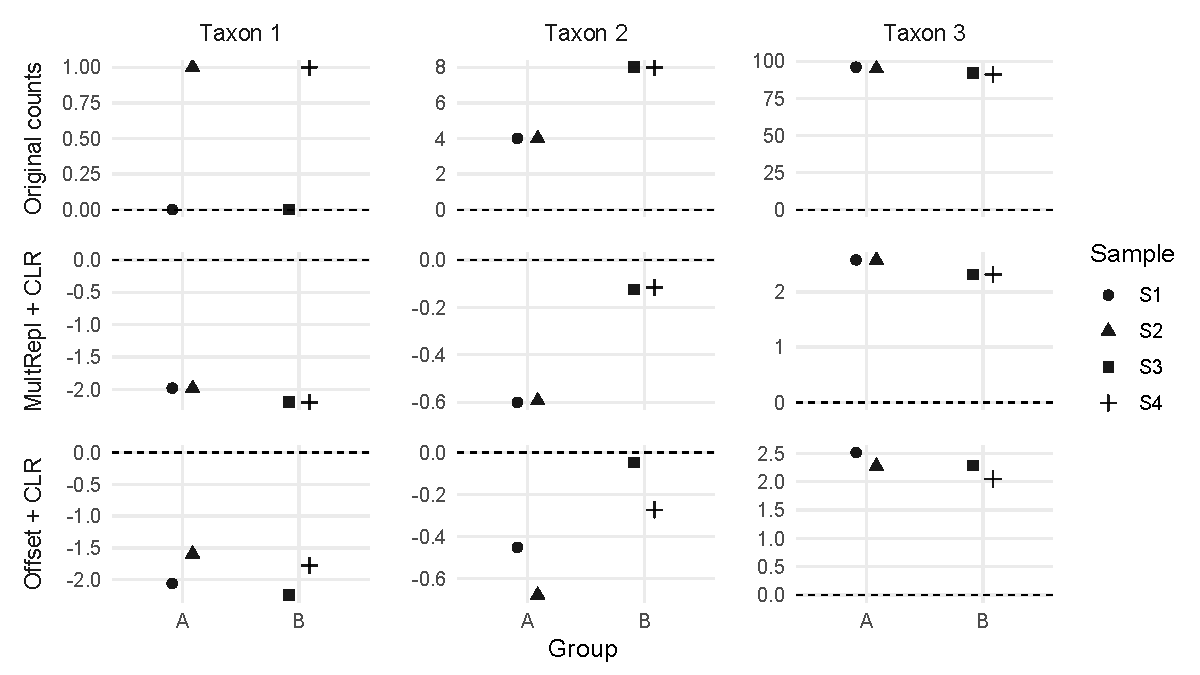
\includegraphics[width=\textwidth]{../ch02_microbiome_data/figures/clr_mini_example/thesis_original_transformed_values-1.pdf}
\caption{\textbf{Visualization of the toy data before and after CLR transformation.} The first row shows the original counts. The second and third rows show CLR-transformed values after multiplicative replacement (``multRepl + CLR'') and additive offset replacement (``Offset + CLR''), respectively. Multiplicative replacement changes positive components only through a proportional rescaling within samples, whereas additive offset replacement adds the same value to all components. Consequently, the transformed values differ not only for the taxon containing zeros, but also for taxa that were positive in all samples.}
\label{fig:2micro:clr_toy_example}
\end{figure}

For \textbf{distance-based analyses}, the relevant object is the geometry between samples in CLR space. Consider the first two samples, which differ by a maximum of one in their original counts. Their CLR distance after multiplicative replacement is
\begin{equation}
\left\|\operatorname{CLR}(x_1^{(M)})-\operatorname{CLR}(x_2^{(M)})\right\|_2 \approx 0.008.
\label{eq:2micro::mult_replacement_distance_example}
\end{equation}
After additive offset replacement, the corresponding distance is
\begin{equation}
\left\|\operatorname{CLR}(x_1^{(+)})-\operatorname{CLR}(x_2^{(+)})\right\|_2 \approx 0.570.
\label{eq:2micro:additive_offset_distance_example}
\end{equation}
Thus, the offset strategy leads to a substantially larger distance between the same two samples. The reason is that additive offset replacement changes ratios among observed components, whereas multiplicative replacement changes positive components only through a proportional rescaling. This example does not imply that multiplicative replacement eliminates the influence of zeros on distances. The replacement value and the sample-specific zero pattern can still affect CLR coordinates. Its advantage is more specific: it preserves ratios among components that were originally observed within a sample. In the toy example, the comparison between S1 and S2 is especially close after multiplicative replacement because both samples have the same total count and the replacement results in almost identical compositions. In real data, samples usually differ in sequencing depth and zero pattern. Therefore, normalization to a common compositional scale and suitable filtering remain important before applying CLR-based distance analyses.

For \textbf{differential distribution analyses}, the transformed values themselves are the objects being compared. Consider taxon 2. After multiplicative replacement followed by CLR, the transformed values are
\begin{equation}
\operatorname{CLR}(x^{(M)})_{\cdot 2}
\approx
(-0.601,\,-0.594,\,-0.124,\,-0.117),
\label{eq:2micro:mult_replacement_taxon2_clr_values}
\end{equation}
whereas after additive offset replacement followed by CLR they are
\begin{equation}
\operatorname{CLR}(x^{(+)})_{\cdot 2}
\approx
(-0.452,\,-0.680,\,-0.046,\,-0.273).
\label{eq:2micro:additive_offset_taxon2_clr_values}
\end{equation}
Thus, the marginal distribution of the CLR-transformed values of taxon 2 differs between the two replacement strategies, even though the same original count table is used. This is relevant for analyses that compare transformed taxon-level distributions across samples or groups.

The same transformed values would also enter a simple feature-level \textbf{differential abundance-style comparison} on the CLR scale. For taxon 2, the difference between the mean transformed value in group $B$ and the mean transformed value in group $A$ is
\begin{equation}
\Delta_2^{(M)}
=
\frac{1}{2}\sum_{k:g_k=B}\operatorname{CLR}(\mathbf{x}_k^{(M)})_2
-
\frac{1}{2}\sum_{k:g_k=A}\operatorname{CLR}(\mathbf{x}_k^{(M)})_2
\approx 0.476
\label{eq:2micro:mult_replacement_da_contrast_example}
\end{equation}
after multiplicative replacement, whereas after additive offset replacement it is
\begin{equation}
\Delta_2^{(+)}
=
\frac{1}{2}\sum_{k:g_k=B}\operatorname{CLR}(\mathbf{x}_k^{(+)})_2
-
\frac{1}{2}\sum_{k:g_k=A}\operatorname{CLR}(\mathbf{x}_k^{(+)})_2
\approx 0.406.
\label{eq:2micro:additive_offset_da_contrast_example}
\end{equation}
This calculation is not intended as a realistic differential abundance test, because the toy data contain only two samples per group. It nevertheless illustrates that the transformed group difference entering such an analysis can depend on the zero-handling strategy before any statistical test is performed. The toy example is balanced in the sense that both groups contain one sample with a zero in taxon 1 and one sample without such a zero. In real data, zero patterns are usually not balanced across samples or groups, so the influence of replacement on group comparisons may be stronger and less transparent.

For \textbf{association and proportionality analyses}, pairwise log-ratios and their variation across samples are central. Consider taxa 2 and 3, which are positive in all four samples. In the original data, the corresponding sample-wise log-ratios are
\begin{equation}
\log\left(\frac{x_2}{x_3}\right)
\approx
(-3.178,\,-3.168,\,-2.442,\,-2.431).
\label{eq:2micro:original_logratio_taxa23_example}
\end{equation}
After multiplicative replacement, the CLR-transformed values of taxa 2 and 3 change because the geometric mean is affected by the zero replacement. However, their coordinate differences remain identical to the original log-ratios:
\begin{equation}
\operatorname{CLR}(x^{(M)})_{\cdot 2}
-
\operatorname{CLR}(x^{(M)})_{\cdot 3}
=
\log\left(\frac{x_2^{(M)}}{x_3^{(M)}}\right)
\approx
(-3.178,\,-3.168,\,-2.442,\,-2.431).
\label{eq:2micro:mult_replacement_logratio_taxa23_example}
\end{equation}
This equality holds because multiplicative replacement rescales originally non-zero components within a sample by the same factor and therefore preserves their ratios. In contrast, after additive offset replacement the corresponding coordinate differences become
\begin{equation}
\operatorname{CLR}(x^{(+)})_{\cdot 2}
-
\operatorname{CLR}(x^{(+)})_{\cdot 3}
=
\log\left(\frac{x_2^{(+)}}{x_3^{(+)}}\right)
\approx
(-2.965,\,-2.955,\,-2.335,\,-2.325).
\label{eq:2micro:additive_offset_logratio_taxa23_example}
\end{equation}
Thus, additive offset replacement changes the log-ratio pattern even for a pair of taxa that contains no zeros. For example, the variance of this log-ratio is approximately $0.181$ in the original data and remains $0.181$ after multiplicative replacement, whereas it decreases to approximately $0.132$ after additive offset replacement. Since association measures, proportionality measures, and network edges can depend on the variation of such log-ratios or transformed taxon profiles across samples, this modification can affect downstream inference.


This example illustrates why multiplicative replacement and additive offset replacement should not be treated as equivalent preprocessing choices. Multiplicative replacement preserves ratios among originally observed components and therefore remains closest to the standard CLR and Aitchison interpretation after zero replacement. Additive offset replacement yields a smoothed complete representation, but it changes ratios among non-zero components and can therefore affect distances, feature-level contrasts, marginal transformed distributions, and association patterns. This does not mean that multiplicative replacement is universally optimal. In particular, between-sample comparisons can still be affected by the replacement value and by sample-specific zero patterns. However, multiplicative replacement avoids additionally perturbing ratios among observed components, whereas additive offset replacement changes such ratios by construction.

The mCLR transformation is not included in this numerical comparison because it is not a replacement strategy in the same sense. It leaves zeros unchanged, centers only the positive components, and applies a sample-specific positive shift to non-zero transformed values. As discussed above, this representation can be appropriate when explicitly required by a method, but it should not be interpreted as an interchangeable substitute for standard CLR in comparative analyses.

The R code generating the tables, numerical values, and Figure~\ref{fig:2micro:clr_toy_example} is included in the thesis repository archived on Zenodo \citep{Peschel2026thesisRepo}. Within this repository, the material for the present section is provided in the folder \href{https://github.com/stefpeschel/phd_thesis/tree/main/ch02_microbiome_data}{\texttt{ch02\_microbiome\_data}}.

%====================================
\section{Statistical consequences of preprocessing}
\label{sec:2micro:preprocessing_consequences}
%====================================

From a statistical perspective, the preprocessing steps discussed in this chapter should not be viewed merely as technical data-cleaning procedures, but as integral components of the analysis strategy. Filtering, zero handling, normalization, and transformation determine the effective data representation on which downstream summaries, models, and hypothesis tests are based. They therefore influence not only numerical stability, but also the inferential target and the interpretation of the results.

Filtering changes both the number of samples and the number of features entering the analysis. Removing low-depth samples can reduce the influence of sampling zeros and stabilize distance-based analyses \citep{weiss2017normalization}, while filtering rare taxa can reduce the influence of features that contribute little information but many sampling zeros. At the same time, taxa filtering changes the subcomposition under study and therefore modifies the feature set and relative reference system on which compositional inference is based \citep{aitchison1986statistical}. This is particularly relevant when conclusions are interpreted as statements about the microbial community as a whole, although the analysis was performed only on a filtered subset of features.

Zero handling introduces additional assumptions because the biological or technical origin of an observed zero is generally not identifiable from the count table alone \citep{martin2011dealing,quinn2019field}. Replacement and imputation strategies determine how unobserved or undetected taxa enter log-ratio coordinates and can therefore affect variances, associations, distances, and network structures. Classical compositional data analysis distinguishes between replacement strategies that preserve the relative structure among observed components and approaches that perturb non-zero components \citep{martin-fernandez2003dealing}. More recently, \citet{tang2026critical} provided a comparison of zero-handling strategies for high-dimensional compositional count data and emphasized that simple replacement rules become less reliable when the proportion of zeros is high. In the settings considered, multiplicative replacement performed well when the zero proportion was moderate, whereas low-rank log-ratio imputation by lrSVD performed more favorably in highly sparse settings. This illustrates that zero handling is not simply a numerical workaround for logarithms, but a modeling decision about how sparse observations are represented statistically.

Normalization and transformation define the scale or coordinate system of the analysis. Scaling-based methods such as total sum scaling address heterogeneous library sizes but make the compositional constraint induced by closure explicit rather than resolving it \citep{weiss2017normalization,aitchison1986statistical}. This is also relevant before zero replacement: although the CLR transformation is scale-invariant for strictly positive data, the replacement value itself is not automatically comparable across samples with different library sizes. Therefore, when a zero-replacement method uses fixed replacement values, the data should first be brought to a common compositional scale, for example by total count normalization or conversion to relative abundances. Alternatively, the replacement procedure must account explicitly for sample-specific totals. Variance-stabilizing transformations primarily target the mean-variance relationship of count data, whereas log-ratio transformations embed compositional observations into Euclidean space and make inference interpretable in terms of ratios \citep{aitchison1986statistical,greenacre2021compositional}. Consequently, the same biological data may lead to different statistical objects depending on the chosen representation: scaled counts, variance-stabilized values, imputed compositions, or log-ratio coordinates.

These choices also affect hypothesis testing and network analysis. Permutation tests require exchangeability under the null hypothesis \citep{good2005permutation,phipson2010permutation}, and preprocessing can change the finite-sample behavior of the test statistic by altering sparsity, variance heterogeneity, or the effective feature space. This is particularly important when preprocessing contains a non-trivial imputation step. If an imputation method is considered part of the statistic, or if it is fitted separately within permuted groups, it should in principle be repeated under each permutation. For computationally intensive methods such as lrSVD, this can make permutation-based workflows substantially more complex. Association network analysis is especially sensitive to these decisions, because edge estimation depends on the conditioning, sparsity, and geometry of the transformed data \citep{kurtz2015sparse}. This motivates workflows that make preprocessing choices explicit and reproducible rather than treating them as hidden defaults.

Taken together, preprocessing defines the retained sample set, the feature space, and the coordinate representation in which community-level summaries, feature-level measures, and association networks are analyzed. It should therefore be understood as part of statistical inference for microbiome data rather than as a separate technical step preceding the actual analysis.

%====================================
\section{Preprocessing choices in this thesis}
\label{sec:2micro:preprocessing_choices_thesis}
%====================================

The preprocessing strategy used in this thesis follows from the statistical perspective outlined above. Preprocessing choices are not treated as neutral technical defaults, but as part of the definition of the data representation used for inference. At the same time, using consistent baseline choices whenever possible improves interpretability across analysis sections. Therefore, this thesis defines a general preprocessing framework that is adapted when required by the downstream analysis. Table~\ref{tab:2micro:preprocessing_choices} gives a compact overview of the default choices used throughout the thesis.

\begin{table}[!ht]
\centering
\caption{\textbf{Preprocessing choices in this thesis.} Summary of the default preprocessing choices used throughout the thesis. The step numbers indicate the default preprocessing order. Deviations from these choices or from this order are stated and justified in the corresponding analysis sections.}
\label{tab:2micro:preprocessing_choices}
\vspace{0.5em}
\renewcommand{\arraystretch}{1.3}
\begin{tabular}{p{4cm}p{10.6cm}}
\toprule
\textbf{Step} & \textbf{Choice in this thesis} \\
\midrule
\textbf{1. Sample filtering} & Remove samples with \textbf{zero total counts}. Apply additional sample filtering if required by the analysis. \\
\textbf{2. Taxa filtering} & Remove taxa with \textbf{zero total counts after sample filtering}. Apply additional prevalence or abundance filtering if required for stable estimation or interpretation. \\
\textbf{3. Aggregation} & Use \textbf{genus-level} aggregation unless stated otherwise. The choice of genus level is motivated in the application chapter after exploratory inspection of the ASV-level data. \\
\textbf{4. Normalization} & Use \textbf{total sum scaling}, i.e. conversion to relative abundances, when a common compositional scale is required. \\
\textbf{5. Zero handling} & Use \textbf{multiplicative replacement} as the default zero-handling strategy before CLR transformation. \\
\textbf{6. Transformation} & Use the \textbf{CLR transformation} for analyses requiring log-ratio coordinates or Aitchison geometry. \\
\bottomrule
\end{tabular}
\end{table}

As a minimal filtering step, samples and taxa with an overall count of zero are removed before analysis. Such samples or taxa do not contribute quantitative information and can lead to undefined quantities in relative abundance, log-ratio, or distance-based analyses. Further filtering is performed in an analysis-specific manner when needed. This is particularly important for highly sparse microbiome data, where zero handling can otherwise dominate the transformed representation. For example, network-based analyses often require more restrictive taxon filtering to obtain smaller and more interpretable networks and to reduce instability caused by extremely sparse taxa,whereas community-level analyses may retain a larger feature set when rare taxa are considered relevant to the chosen community summary. Thus, filtering is not fixed globally beyond the removal of empty samples and taxa, but is chosen according to the statistical and interpretational requirements of the analysis.

Taxonomic aggregation is also treated as an analysis decision rather than as a purely technical simplification. In this thesis, genus-level aggregation is used as the default representation unless stated otherwise. This choice provides a compromise between biological resolution and statistical stability. In the PASTURE application, the decision to work at genus level is made after an exploratory description of the ASV-level data and the sparsity structure across taxonomic levels.

For the CLR-based workflow used in this thesis, the data are first brought to a common compositional scale by total sum scaling, or equivalently by conversion to relative abundances, before multiplicative replacement is applied. This step ensures that the replacement value has a comparable compositional meaning across samples with different sequencing depths. After this normalization step, multiplicative replacement followed by CLR transformation is used as the default representation, unless a different zero-handling strategy is explicitly motivated by the downstream method or analysis target. This choice is motivated by Sections~\ref{sec:2micro:zeros:replacement} and~\ref{sec:2micro:clr_with_zeros}. Multiplicative replacement makes the CLR transformation applicable to sparse data while preserving ratios among originally non-zero components. This property is important because differences between CLR coordinates are pairwise log-ratios, and many analyses considered in this thesis depend directly or indirectly on such log-ratio relationships. For Aitchison-distance-based analyses, the transformed values define the geometry between samples. For exploratory feature-level analyses conducted on the CLR scale, the transformed values define taxon-specific marginal distributions or group contrasts. For proportionality analyses and several compositional association approaches, log-ratio relationships and their variation across samples are central.

This default should not be interpreted as a claim that multiplicative replacement is universally optimal. In very sparse data sets, more elaborate imputation approaches such as lrSVD may exploit low-rank structure across samples and taxa and may perform better than simple replacement rules \citep{tang2026critical}. However, lrSVD introduces additional modeling assumptions and tuning choices, including the choice of rank and the treatment of bounds for censored or missing values. It also complicates permutation-based analyses, which are a central methodological theme of this thesis. When lrSVD is estimated from the analyzed data, it should generally be repeated within each permutation so that the permutation procedure reflects the complete analysis pipeline. In the permutation-intensive analyses considered in this thesis, this would substantially increase computational cost and add an additional methodological layer outside the present scope. For this reason, lrSVD is discussed as an important alternative for highly sparse compositional count data, but it is not used as the primary zero-handling strategy here.

Other alternatives are also interpreted more narrowly. Offset-based CLR transformations motivated by the extended geometric mean provide a smoothed complete representation and may reduce extreme zero-induced transformed values. However, as discussed in Section~\ref{sec:2micro:clr_with_zeros}, the extended geometric mean does not by itself solve the zero problem of the CLR transformation, because the component-wise logarithms remain undefined for zero entries. Using the resulting offset as an additive replacement makes the transformation computable, but changes ratios among components that were originally non-zero. The comparative example in Section~\ref{sec:2micro:clr_with_zeros} illustrates how this can affect distances, transformed marginal values, group contrasts, and log-ratio variation. Therefore, global offset-based transformations are not used as the primary representation when a standard log-ratio or Aitchison interpretation is required. Similarly, mCLR preserves zeros and can be appropriate when a method explicitly assumes this representation, but it is not treated as an interchangeable substitute for standard CLR because positive-part centering and the sample-specific shift alter coordinate differences and cross-sample marginal distributions.

Accordingly, the analyses in this thesis use a consistent baseline preprocessing strategy: empty samples and taxa are removed, genus-level aggregation is used unless stated otherwise, data are converted to relative abundances before zero replacement for CLR-based analyses, and multiplicative replacement followed by CLR transformation is used as the default for CLR-based analyses. Deviations from this baseline are stated and justified in the corresponding analysis sections, for example when stricter filtering is required for interpretability, when a method prescribes its own preprocessing, or when an alternative representation is used for sensitivity or exploratory purposes. Results are therefore interpreted conditional on the retained feature set, the chosen taxonomic resolution, and the preprocessing strategy used for the respective analysis.

% !TeX root = ../thesis.tex

%%%%%%%%%%%%%%%%%%%%%%%%%%%%%%%%%%%%%
\thesischapter[ch:community][0.7\textwidth]
  {``The whole is something else than the sum of its parts.''}
  {--- Kurt Koffka, 1935}
  {Community-level summaries}
\nocite{koffka1935principles}
\chapterabstract{This chapter introduces the first of the three analysis target levels considered in this thesis: community-level summaries. Rather than focusing on individual taxa or pairwise associations, these methods reduce characteristic properties of the microbial community to interpretable summary quantities, either at the level of a single sample or for an entire population. Within-sample diversity, between-sample dissimilarity, community dispersion, regression for compositional responses, and compositional equivalence provide complementary views on global microbiome variation. The chapter establishes the methodological foundation for the community-level part of the integrated analysis in Chapter~\ref{ch:application}.}
\chaptercontents
%%%%%%%%%%%%%%%%%%%%%%%%%%%%%%%%%%%%%

%%%%%%%%%%%%%%%%%%%%%%%%%%%%%%%%%%%%%
\section{Introduction}
\label{sec:3community:intro}
%%%%%%%%%%%%%%%%%%%%%%%%%%%%%%%%%%%%%

This chapter considers community-level analyses, in which the microbial community is summarized or modeled as a whole rather than through individual taxa or pairwise associations. Such analyses provide complementary perspectives on global community structure and are often used to assess whether microbial communities differ across samples, groups, or environmental conditions.

Community-level approaches can be distinguished by the statistical object they summarize. Within-sample diversity measures, commonly referred to as alpha diversity, reduce each sample to a scalar quantity describing characteristics such as richness, evenness, or dominance. Between-sample dissimilarities, often discussed under the term beta diversity, quantify differences between pairs of samples and thereby represent the structure of an entire sample collection through a distance or dissimilarity matrix. These dissimilarities form the basis for ordination, distance-based group comparisons such as PERMANOVA, and analyses of community dispersion. A further perspective is provided by regression models for compositional responses, in which the transformed microbial composition is modeled directly as a multivariate outcome. Finally, compositional equivalence testing addresses a complementary inferential question by assessing whether group differences are sufficiently small to be regarded as practically negligible.

The appropriate representation of the data depends on the method under consideration. As discussed in Chapter~\ref{ch:microbiome}, microbiome count data are compositional, sparse, and characterized by heterogeneous library sizes. Some community-level methods, such as model-based richness estimation, are designed to account for unequal sampling depth and uncertainty due to unobserved taxa and can therefore operate directly on count data. Other approaches require a transformation or dissimilarity measure that is compatible with the relative nature of the observations. These choices determine the statistical object under study and consequently affect the interpretation of diversity estimates, distances, regression coefficients, and group comparisons.

The chapter is organized into four parts. Section~\ref{sec:3community:within_sample_div} introduces within-sample diversity measures, including richness, Shannon diversity, and Gini--Simpson diversity, together with methods for group comparison and regression modeling. Section~\ref{sec:3community:between_sample_diss} considers between-sample dissimilarities, with particular emphasis on Bray--Curtis dissimilarity and Euclidean distance after centered log-ratio transformation. These quantities are subsequently used for ordination, PERMANOVA, and the assessment of group differences in multivariate dispersion. Section~\ref{sec:3community:regression} discusses regression models for compositional responses, whereas Section~\ref{sec:3community:compositional_equivalence} introduces compositional equivalence testing as an alternative to conventional difference testing.

Together, these methods characterize community structure at complementary resolutions: within-sample diversity summarizes individual samples, between-sample dissimilarities describe relationships among samples, compositional-response regression relates covariates to the community profile, and equivalence testing evaluates whether group-level compositional differences are practically small. They form the community-level component of the integrated analysis in Chapter~\ref{ch:application}.


%%%%%%%%%%%%%%%%%%%%%%%%%%%%%%%%%%%%%
\section{Within-sample diversity}
\label{sec:3community:within_sample_div}
%%%%%%%%%%%%%%%%%%%%%%%%%%%%%%%%%%%%%

\begin{figure}[H]
\centering
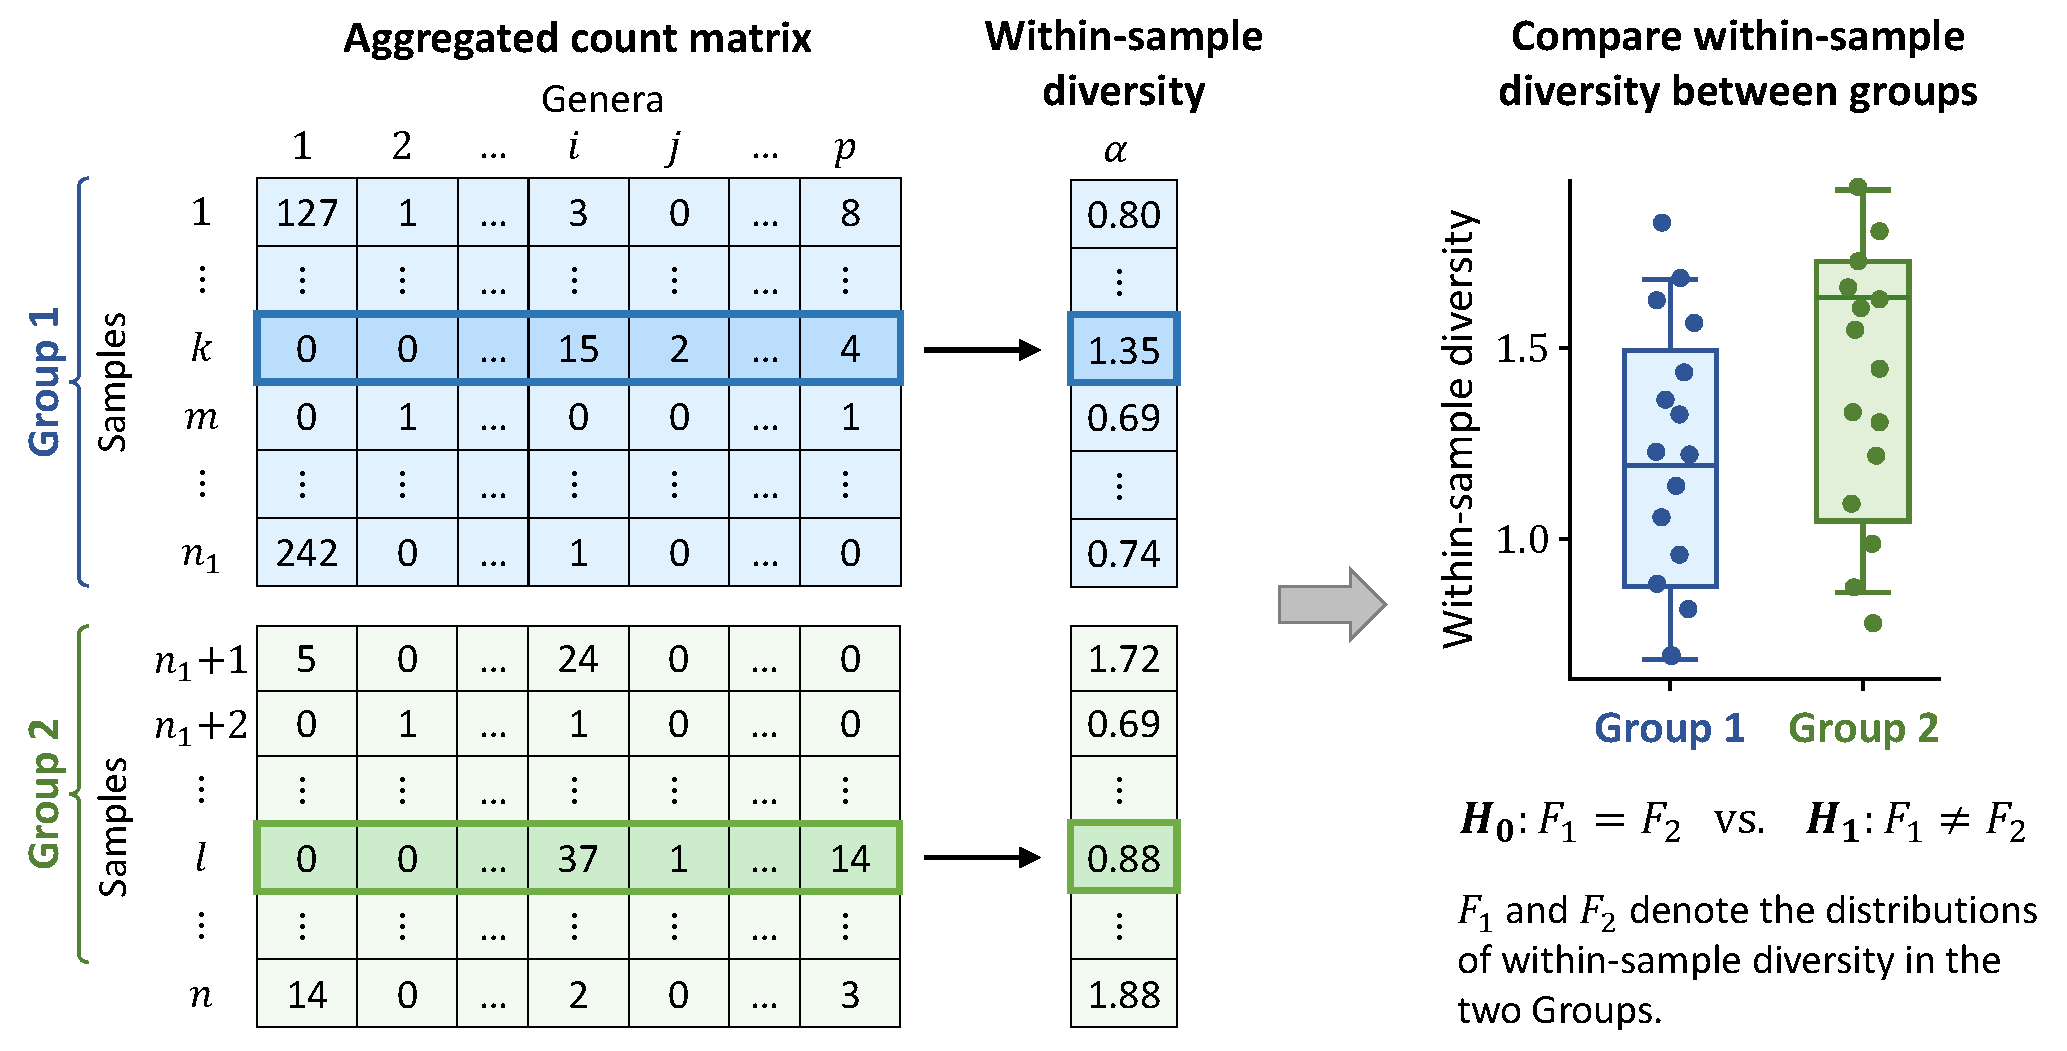
\includegraphics[width=\textwidth]{../ch03_community_level/overview_figures/overview_alpha.pdf}
\caption{\textbf{Overview of within-sample diversity analysis.} The unfiltered taxonomically aggregated count matrix, with samples in rows and taxa in columns, serves as the input for within-sample diversity analysis. Summarizing counts across taxa yields one diversity value per sample, for example an alpha-diversity measure. These sample-level values can then be compared between groups using parametric or non-parametric tests.}
\label{fig:3community:overview_alpha_diversity}
\end{figure}

Within-sample diversity, commonly referred to as \emph{alpha diversity}, describes the diversity of the microbial community observed within an individual sample. Alpha diversity measures reduce the high-dimensional taxonomic composition of each sample to a scalar quantity and therefore represent community-level summaries in the framework of analysis targets introduced in Chapter~\ref{ch:introduction}. Because they yield one value per sample, these measures are widely used in exploratory analyses, group comparisons, and regression settings, where the diversity estimate serves as the response variable.

Different alpha diversity measures emphasize different aspects of within-sample community structure. Richness measures quantify the number of taxa present, whereas diversity indices additionally account for the distribution of abundances across taxa. The Shannon index and the Gini--Simpson index are examples of such entropy- and dominance-based indices, respectively. As discussed in Chapter~\ref{ch:microbiome}, microbiome data are characterized by finite and heterogeneous sampling depth, sparsity, and a large proportion of rare taxa. These features have important implications for the estimation and comparison of alpha diversity, in particular for richness, which is sensitive to unobserved taxa and sampling effort.

To address these challenges, we focus on model-based approaches to diversity estimation that explicitly account for unequal sampling depth and the presence of unobserved taxa. In particular, we consider richness estimation via the \texttt{breakaway} framework and entropy-based diversity estimation using \texttt{DivNet}. These methods provide estimates together with uncertainty measures, which enables statistical comparison and regression modeling without relying on procedures such as rarefaction that modify the observed count matrix.

In the following, we first introduce richness estimation and then discuss diversity indices that incorporate abundance distributions. We then describe approaches for statistical comparison and regression modeling based on these sample-level community summaries. Figure~\ref{fig:3community:overview_alpha_diversity} provides a schematic overview of the workflow for estimating and comparing within-sample diversity across groups.


%====================================
\subsection{Richness estimation}
\label{sec:3community:within:richness}
%====================================

Richness is a basic measure of alpha diversity and is defined as the number of distinct taxa present in a sample. In the context of microbiome data, richness aims to quantify how many microbial features, such as amplicon sequence variants (ASVs), are represented in a community. Formally, for a sample $k$, the observed richness is given by
\begin{equation}
\alpha_{\mathrm{rich}, k}^{\mathrm{obs}} = \sum_{i=1}^p \mathbb{I}(x_{ki} > 0),
\end{equation}
where $\mathbb{I}(\cdot)$ denotes the indicator function. However, under incomplete sampling, the observed number of taxa typically underestimates the richness of the underlying community because low-abundance taxa may remain unobserved.

As discussed in Chapter~\ref{ch:microbiome}, microbiome data are characterized by high sparsity and a large proportion of rare taxa. Many taxa occur at low abundance and may not be observed in all samples, particularly when sequencing depth is limited. As a result, the naive richness estimator tends to underestimate the true richness, and comparisons across samples are confounded by differences in sampling effort.

To address these challenges, we focus on approaches to diversity estimation that account for unequal sampling depth and the presence of unobserved taxa. As discussed in Section~\ref{sec:2micro:norm:rarefaction}, rarefaction provides a simple and widely used strategy to equalize library sizes by subsampling counts to a common depth, and is often employed in diversity and distance-based analyses. However, rarefaction achieves comparability by discarding observed counts and therefore comes at the cost of information loss, which is particularly consequential for richness estimation where rare taxa play a central role.

An alternative approach is proposed by \citet{willis2015estimating}, who estimate the number of unobserved taxa rather than reducing the observed data through subsampling. In particular, we consider richness estimation via the \texttt{breakaway} framework and entropy-based diversity measures estimated with \texttt{DivNet}. These methods provide model-based estimates and associated uncertainty measures, facilitating comparisons of diversity across samples and groups without relying on rarefaction. Conceptually, this shifts the treatment of heterogeneous sampling depth from a preprocessing step to an explicit component of the statistical model, where uncertainty due to incomplete sampling is directly accounted for in the estimation.

For a given sample $k$, let $n_j^{(k)}$ denote the number of taxa observed exactly $j$ times, that is,
\begin{equation}
n_j^{(k)} = \#\{i : x_{ki} = j\}.
\end{equation}
The total richness can then be written as
\begin{equation}
\alpha_{\mathrm{rich}, k} = \sum_{j \geq 0} n_j^{(k)},
\end{equation}
where $n_0^{(k)}$ denotes the number of unobserved taxa. The estimation problem therefore reduces to predicting $n_0^{(k)}$. Here, the notion of an unobserved taxon is defined relative to the feature universe represented by the sequencing and preprocessing workflow, not to all microbial taxa that could in principle occur in the sampled environment.

The approach of \citet{willis2015estimating} models the ratios of adjacent frequency counts,
\begin{equation}
\frac{n_{j+1}^{(k)}}{n_j^{(k)}},
\end{equation}
as a function of $j$, motivated by classical characterizations of discrete distributions via adjacent probability ratios. In particular, a broad class of distributions can be represented through probability ratios that take the form of rational functions in $j$, providing a flexible modeling framework beyond traditional assumptions such as mixed Poisson models. A nonlinear regression model is fitted to the observed ratios, accounting for their sampling variability through appropriate weighting, and subsequently extrapolated to $j = 0$ to estimate the ratio $n_1^{(k)} / n_0^{(k)}$, from which the number of unobserved taxa is obtained. The resulting richness estimate is given by
\begin{equation}
\hat{\alpha}_{\mathrm{rich}, k} = \sum_{j \geq 1} n_j^{(k)} + \hat{n}_0^{(k)}.
\end{equation}

The \texttt{breakaway} R package provides a practical implementation of this framework using a finite set of low-order ratio models, weighted nonlinear least squares fitting, and a data-driven model selection procedure. Standard errors are obtained via a delta-method approximation. Compared to naive richness estimates, this approach explicitly accounts for rare and unobserved taxa and does not require rarefaction, as differences in sampling depth are incorporated into the modeling framework.

%====================================
\subsection{Diversity indices}
\label{sec:3community:within:diversity}
%====================================

In addition to richness, alpha diversity measures often incorporate information on the relative abundances of taxa within a community. While richness quantifies the number of distinct taxa present, it treats all taxa equally and ignores how sequencing counts are distributed among them. As a result, two communities with the same richness may differ substantially in their ecological structure, for example if one is dominated by a few highly abundant taxa while the other exhibits a more even distribution. Such differences are particularly relevant in microbiome studies, where communities are typically characterized by a small number of dominant taxa and a long tail of low-abundance taxa. Therefore, diversity measures that account for relative abundances provide a more informative summary of community structure beyond mere presence or absence.

Let $z_{ki} \in [0,1]$ denote the (unknown) relative abundance of taxon $i$ in sample $k$, such that $\sum_{i=1}^p z_{ki} = 1$. The Shannon entropy is defined as
\begin{equation}
\label{eq:3community:shannon}
\alpha_{\mathrm{Sh}, k} = - \sum_{i=1}^p z_{ki} \log(z_{ki}),
\end{equation}
and captures both richness and evenness of the community \citep{willis2018divnet}. For a fixed number of taxa, the Shannon index is maximized when all taxa are equally abundant and decreases as the distribution becomes more uneven. In particular, it places relatively high weight on low-abundance taxa.

Following \citet{willis2018divnet}, the Simpson index is defined as
\begin{equation}
\label{eq:3community:simpson}
\alpha_{\mathrm{Si}, k} = \sum_{i=1}^p z_{ki}^2.
\end{equation}
It can be interpreted as the probability that two randomly drawn individuals from the community belong to the same taxon. In contrast to the Shannon entropy, the Simpson index is less sensitive to rare taxa and primarily reflects dominance structure within the community.

In practice, the relative abundances $z_{ki}$ are not directly observed. A common approach is to estimate them by empirical proportions,
\begin{equation}
\hat{z}_{ki}^{\mathrm{plug-in}} = \frac{x_{ki}}{m_k},
\end{equation}
yielding plug-in estimators of the diversity indices. However, such estimators are known to be biased, particularly in the presence of sparse data and unobserved taxa, which are common in microbiome studies \citep{willis2018divnet}.

To address these limitations, \citet{willis2018divnet} proposed \texttt{DivNet}, which estimates diversity indices based on a model for the underlying compositional structure of the data. The methodology is implemented in the \texttt{DivNet} R package, which provides functions for model fitting, diversity estimation, and uncertainty quantification. Rather than treating samples independently, \texttt{DivNet} models log-ratios of relative abundances across samples using a multivariate normal distribution, thereby accounting for covariance in the log-ratio representation and borrowing strength across samples.

More specifically, let $\mathbf{z}_k \in \mathcal{S}^{p-1}$ denote the latent relative abundance vector for sample~$k$. \texttt{DivNet} assumes that log-ratios of $\mathbf{z}_k$ follow a multivariate normal model with mean depending on covariates and covariance capturing dependence between taxa. Based on the fitted model, an estimate $\hat{\mathbf{z}}_k$ of the latent composition is obtained. The diversity indices are then evaluated by substituting $\hat{z}_{ki}$ into Equations~\eqref{eq:3community:shannon} and~\eqref{eq:3community:simpson}.

A key advantage of this approach is that it estimates diversity at the level of the underlying compositional structure rather than directly from the observed counts, allowing information to be shared across samples and improving estimation accuracy, especially in high-dimensional and sparse settings. Furthermore, by modeling log-ratio transformed abundances jointly across taxa, the approach accounts for dependence structures that are ignored by plug-in estimators.

%====================================
\subsection{Testing within-sample diversity}
\label{sec:3community:within:testing}
%====================================

The diversity measures introduced above yield one scalar value per sample and can therefore be analyzed using standard statistical methods for scalar outcomes. In the context of group comparisons, the primary objective is to assess whether diversity differs across levels of a categorical covariate.

A commonly used nonparametric approach is the Kruskal--Wallis test, which evaluates the null hypothesis
\begin{equation}
H_0: F_1 = F_2 = \cdots = F_G,
\end{equation}
where $F_g$ denotes the distribution of the diversity measure in group $g = 1,\dots,G$. In the case of two groups, this reduces to the Wilcoxon rank-sum test. These tests are based on rank statistics and rely on asymptotic approximations for significance assessment.

As an alternative, permutation-based tests provide a flexible framework that does not rely on distributional assumptions. Let $\hat{\alpha}_k$ denote a diversity estimate for sample $k$, and let $g_k \in \{1,\dots,G\}$ denote the corresponding group label. A test statistic $T = T(\{\hat{\alpha}_k, g_k\}_{k=1}^n)$ is computed for the observed data, for example the Kruskal-Wallis statistic or a difference in group means or medians. Under the null hypothesis and an exchangeable study design, the labels $g_k$ can be permuted to approximate the null distribution of $T$. The corresponding empirical $p$-value is given by
\begin{equation}
p_{\mathrm{emp}} = \frac{1 + \sum_{b=1}^B \mathbb{I}(T_b^* \geq T_{\mathrm{obs}})}{1 + B},
\end{equation}
where $T_{\mathrm{obs}}$ denotes the observed test statistic and $T_b^*$ the statistic obtained from the $b$-th permutation.

As discussed in Chapter~\ref{ch:permapprox}, empirical $p$-values lie on a coarse grid when only a limited number of permutations $B$ can be performed. In the present setting, this limitation is often less critical because alpha diversity analysis usually involves only one or a small number of tests, so that the multiplicity burden is substantially smaller than in high-dimensional feature-level analyses. In contrast to high-dimensional settings with many simultaneous tests, the coarse resolution of empirical $p$-values therefore has limited impact on inference. However, if a finer resolution of $p$-values is desired without substantially increasing the number of permutations, the empirical permutation distribution can be refined by tail approximation methods such as the approach implemented in \texttt{permApprox} (Chapter~\ref{ch:permapprox}).


%====================================
\subsection{Regression modeling of within-sample diversity}
\label{sec:3community:within:regression}
%====================================

\begin{figure}[H]
	\centering
	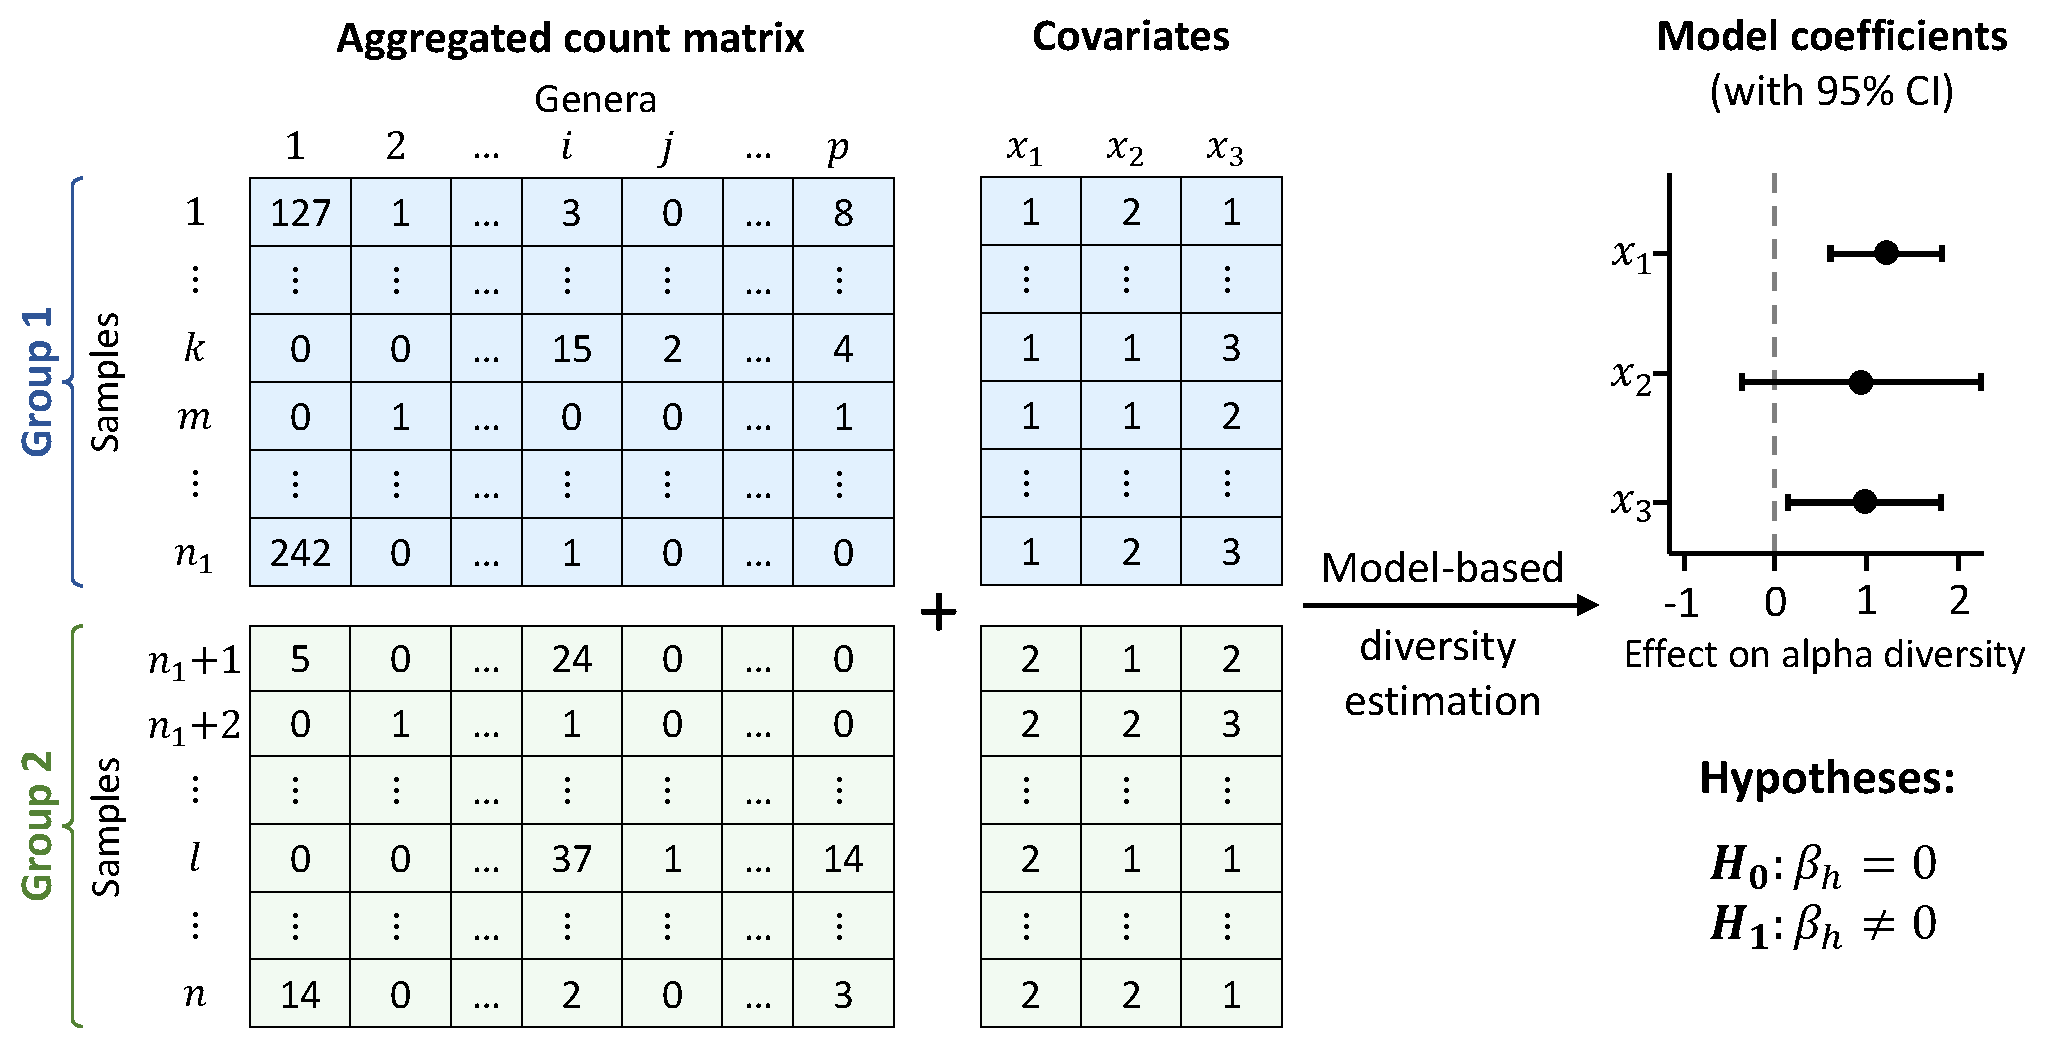
\includegraphics[width=\textwidth]{../ch03_community_level/overview_figures/overview_divnet.pdf}
	\caption{\textbf{Overview of regression-based within-sample diversity analysis.} The unfiltered taxonomically aggregated count matrix and sample-level covariates serve as input for model-based diversity estimation and regression. Methods such as \texttt{breakaway} and \texttt{DivNet} estimate within-sample diversity while accounting for incomplete sampling and, in the case of \texttt{DivNet}, covariance in the log-ratio representation across samples. The resulting regression coefficients quantify associations between covariates and the underlying diversity parameter and can be accompanied by confidence intervals and hypothesis tests.}
	\label{fig:3community:overview_divnet}
\end{figure}

Beyond group comparisons, alpha diversity measures can be analyzed within a regression framework to assess associations with covariates and to adjust for potential confounding factors. In this setting, the diversity measure serves as a response variable, while explanatory variables may include clinical, environmental, or technical factors.

A straightforward approach is to treat the estimated diversity values $\hat{\alpha}_k$ as observed responses and apply standard regression models. Let $\hat{\alpha}_k$ denote the estimated alpha diversity for sample $k$, and let $\mathbf{x}_k$ be a vector of covariates. A simple linear regression model is then given by
\begin{equation}
\hat{\alpha}_k = \beta_0 + \mathbf{x}_k^\top \boldsymbol{\beta} + \varepsilon_k,
\end{equation}
where $\boldsymbol{\beta}$ are regression coefficients and $\varepsilon_k$ is an error term with conditional mean zero given the covariates. Inference is typically based on testing hypotheses of the form $H_0:\beta_h = 0$, where $h$ indexes the covariates, corresponding to the absence of an association between the covariate $x_{kh}$ and the diversity measure.

While this approach is easy to implement and widely used in practice, it implicitly treats the diversity estimates as error-free observations. However, as discussed above, alpha diversity measures are themselves estimated quantities and may exhibit substantial uncertainty, particularly in the presence of sparse data and unobserved taxa.

To account for this, a more principled approach is provided by the model-based framework of \citet{willis2017improved}, which incorporates estimation uncertainty directly into the regression model. Let $\hat{\alpha}_k$ denote a diversity estimate together with its estimated standard error. The model assumes
\begin{equation}
\hat{\alpha}_k = \beta_0 + \mathbf{x}_k^\top \boldsymbol{\beta} + u_k + \varepsilon_k,
\end{equation}
where $u_k$ captures biological variability between samples and $\varepsilon_k$ represents estimation error, whose variance is assumed to be known or estimated from the diversity estimation procedure. Inference is again based on hypotheses of the form $H_0: \beta_h = 0$, with the regression model targeting the underlying diversity parameter while accounting for uncertainty in its estimated sample-level values.

This framework, originally developed for richness estimation, applies more generally to diversity measures for which standard errors are available. In particular, it can be combined with richness estimates obtained via \texttt{breakaway} as well as entropy-based diversity measures estimated using \texttt{DivNet}. The resulting procedure is implemented in the \texttt{breakaway} R package via the \texttt{betta} function. A schematic overview of this model-based regression framework is shown in Figure~\ref{fig:3community:overview_divnet}.

In contrast to the naive regression model, which ignores estimation uncertainty, the model-based approach separates biological variability from measurement error and can lead to more reliable inference when diversity estimates are noisy. However, it relies on additional assumptions, including approximate normality of the diversity estimates and accurate estimation of their standard errors.



%%%%%%%%%%%%%%%%%%%%%%%%%%%%%%%%%%%%%
\section{Between-sample dissimilarity}
\label{sec:3community:between_sample_diss}
%%%%%%%%%%%%%%%%%%%%%%%%%%%%%%%%%%%%%

Within-sample diversity, as introduced in the previous section, summarizes each microbial community by one scalar quantity per sample. Many questions in microbiome analysis, however, concern how microbial communities differ \emph{between} samples. This complementary perspective is based on pairwise comparisons of taxon profiles and leads to an $n \times n$ dissimilarity matrix rather than to a single value per sample. Figure~\ref{fig:3community:overview_beta_diversity} illustrates this general workflow. In the following, we first introduce between-sample dissimilarities as community-level summaries and clarify their relationship to the ecological concept of beta diversity. We then discuss two commonly used choices of dissimilarity, Bray--Curtis dissimilarity and Euclidean distance after log-ratio transformation, before turning to ordination, PERMANOVA, and tests for differences in community dispersion.

\begin{figure}[H]
	\centering
	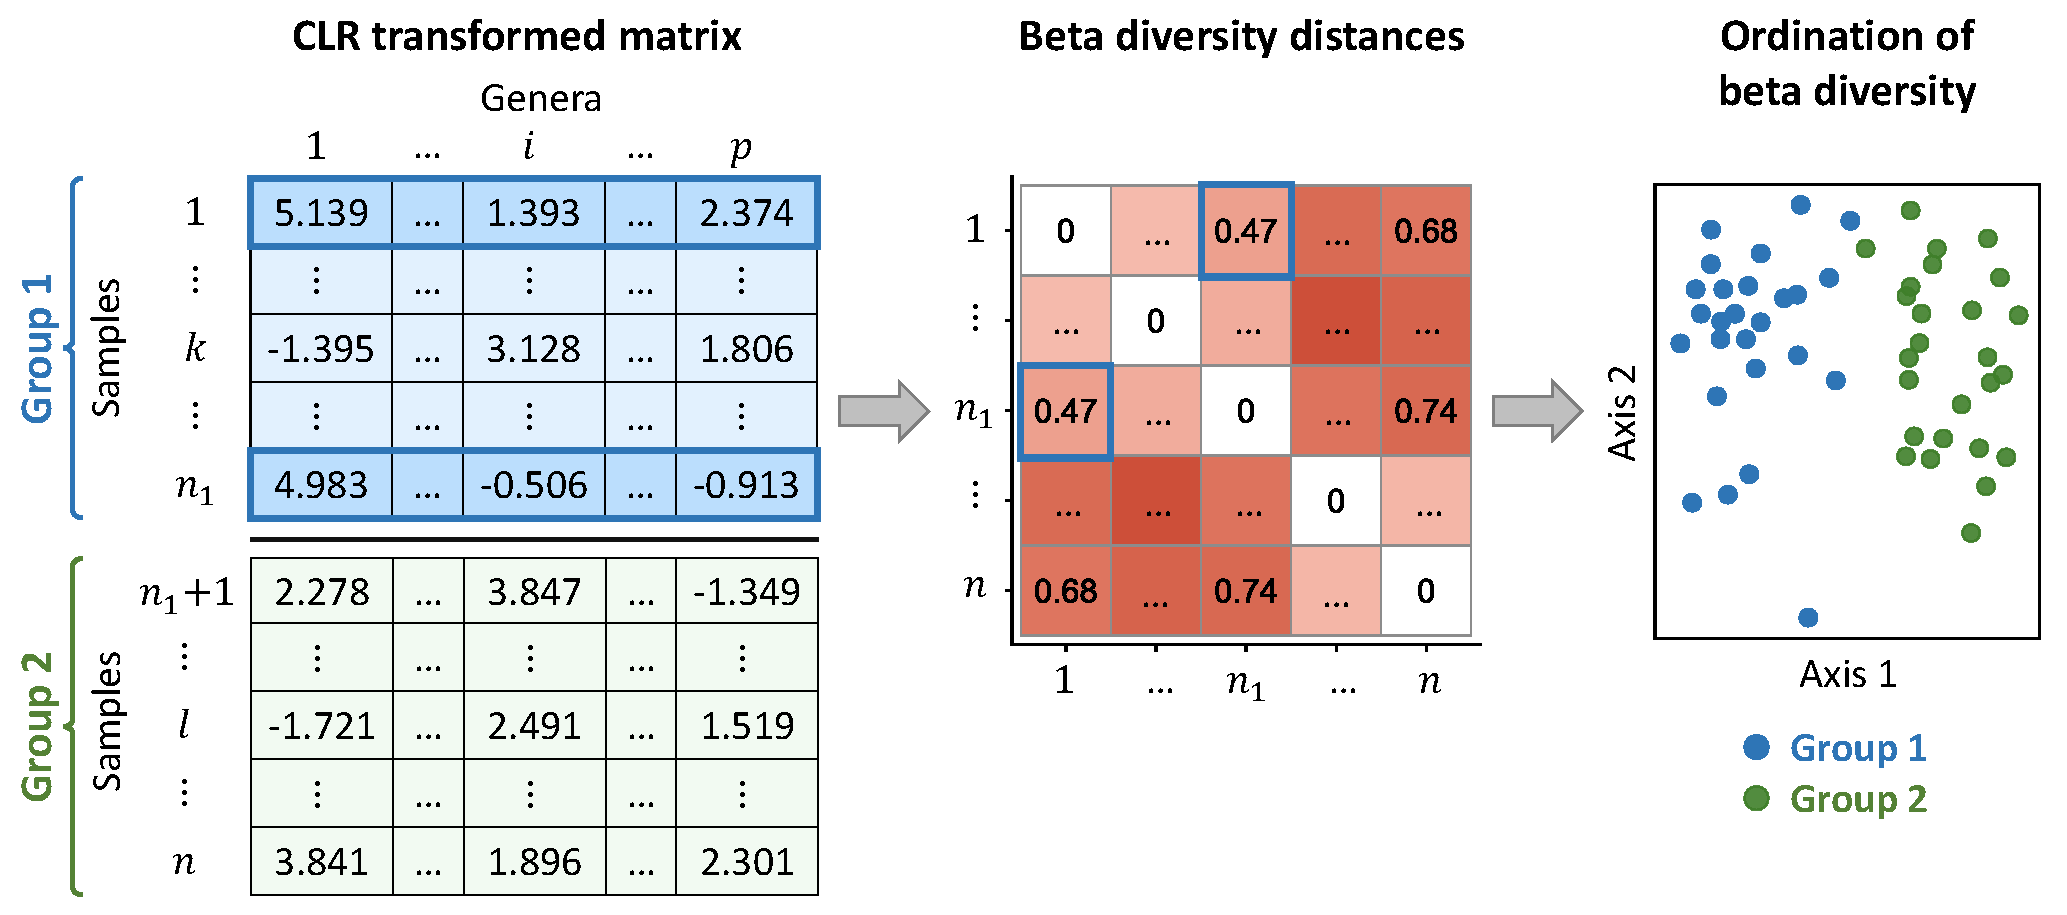
\includegraphics[width=\textwidth]{../ch03_community_level/overview_figures/overview_beta.pdf}
	\caption{\textbf{Overview of between-sample diversity analysis.} After zero handling and CLR transformation, the transformed count matrix is represented by a sample-by-sample distance matrix, here, Euclidean distances between CLR coordinates correspond to Aitchison distances. The resulting beta-diversity distances quantify compositional dissimilarity between samples and can be explored by ordination or used for distance-based group comparisons such as PERMANOVA and PERMDISP.}
	\label{fig:3community:overview_beta_diversity}
\end{figure}

%====================================
\subsection{Beta diversity as a dissimilarity-based summary}
\label{sec:3community:between:beta}
%====================================

In ecology, \emph{beta diversity} describes variation in community composition among sampling units \citep{whittaker1960vegetation,anderson2011navigating}. Since microbiome data also represent communities of co-occurring organisms observed across samples, the same conceptual framework is commonly applied in microbiome studies. In practice, beta diversity is typically represented through pairwise dissimilarities between samples. In this thesis, we use the term between-sample dissimilarity when referring to the statistical object underlying these analyses, namely a pairwise matrix derived from the taxon profiles of all samples.

Let $\mathbf{x}_k=(x_{k1},\ldots,x_{kp})^\top$ and $\mathbf{x}_l=(x_{l1},\ldots,x_{lp})^\top$ denote the taxon profiles of two samples $k$ and $l$. A dissimilarity or distance function $d(\cdot,\cdot)$ assigns a non-negative value $d(\mathbf{x}_k,\mathbf{x}_l)$ to this pair, where smaller values indicate more similar microbial communities and larger values indicate stronger differences. Applying $d$ to all sample pairs yields an $n \times n$ dissimilarity matrix $\mathbf{D}=(d_{kl})$, with entries $d_{kl}=d(\mathbf{x}_k,\mathbf{x}_l)$. For the measures considered here, $\mathbf{D}$ is symmetric and has zeros on the diagonal.

The matrix $\mathbf{D}$ is a community-level summary because each entry aggregates information across all taxa in the two samples being compared. It retains information about which samples are similar to each other, whether samples form clusters, whether groups appear separated, and whether individual samples are unusually dissimilar from the rest of the cohort. This makes between-sample dissimilarities central to exploratory analyses of global community structure.

\newpage
Beta diversity is not a single uniquely defined quantity. The numerical value and interpretation of $d(\mathbf{x}_k,\mathbf{x}_l)$ depend on the chosen dissimilarity measure and on the data representation to which it is applied. Some measures emphasize differences in relative abundance profiles, whereas others compare samples in log-ratio coordinates. Some measures are dominated by abundant taxa, whereas others are more sensitive to changes among rare taxa or to presence--absence patterns. Consequently, different dissimilarities can highlight different aspects of the same count matrix. The choice of dissimilarity should therefore be guided by the scientific question, the preprocessing strategy, and the statistical properties of the data.

For microbiome sequencing data, the compositional nature of the observations is particularly important. Since the total number of reads per sample is constrained by the sequencing process, raw counts and proportions do not represent unconstrained multivariate observations (cf. Section~\ref{sec:2micro:characteristics}). Applying Euclidean distance directly to raw counts or relative abundances may therefore lead to distances that partly reflect library size differences or closure-induced dependencies rather than meaningful biological differences. Distance-based summaries for microbiome data should thus either use dissimilarities whose interpretation is explicitly tied to relative abundance profiles or rely on transformations that embed the compositions into an appropriate Euclidean space.

In the following subsections, we focus on two distance-based summaries that represent these two perspectives. Bray--Curtis dissimilarity is introduced as an ecological measure for comparing abundance profiles and is often applied to relative abundance data. Euclidean distance after centered log-ratio transformation, in contrast, corresponds to the Aitchison distance and is motivated by the log-ratio geometry of compositional data. In this thesis, CLR-based distances are combined with the zero-aware transformation choices discussed in Chapter~\ref{ch:microbiome} to obtain a representation suitable for sparse microbiome profiles.


%====================================
\subsection{Bray--Curtis dissimilarity}
\label{sec:3community:between:bray-curtis}
%====================================

The Bray--Curtis dissimilarity index, originally introduced by \citet{bray1957ordination}, is one of the most widely used measures for comparing ecological community profiles. For two samples $k$ and $l$ with taxon profiles $\mathbf{x}_k=(x_{k1},\ldots,x_{kp})^\top$ and $\mathbf{x}_l=(x_{l1},\ldots,x_{lp})^\top$, it is defined as
\begin{equation}
d_{\mathrm{BC}}(\mathbf{x}_k,\mathbf{x}_l)=\frac{\sum_{i=1}^p |x_{ki}-x_{li}|}{\sum_{i=1}^p (x_{ki}+x_{li})}.
\end{equation}
If $\mathbf{x}_k$ and $\mathbf{x}_l$ are relative abundance vectors with equal total sum, this expression can also be written as
\begin{equation}
d_{\mathrm{BC}}(\mathbf{x}_k,\mathbf{x}_l)=\frac{1}{2}\sum_{i=1}^p |x_{ki}-x_{li}|,
\end{equation}
which shows its close connection to the $L_1$ distance (Manhattan distance) between relative abundance profiles. The dissimilarity takes values between $0$ and $1$, where $0$ indicates identical profiles and increasing values indicate increasingly dissimilar communities.

A useful property of Bray--Curtis dissimilarity is that it ignores joint absences. Taxa that are absent from both samples do not contribute to either the numerator or the denominator. This is desirable in sparse ecological data, because two samples should not be regarded as similar merely because many taxa are absent from both of them. In microbiome data, where the feature table often contains many zero entries, this property makes Bray--Curtis dissimilarity attractive for exploratory comparisons of community composition.

At the same time, Bray--Curtis dissimilarity is strongly influenced by taxa with large relative abundances. Differences in dominant taxa contribute more to the distance than differences among rare taxa. This can be advantageous when the scientific focus lies on abundant community members that drive large-scale compositional differences, but it also means that changes in low-abundance taxa may have little impact on the resulting distance matrix. The interpretation of Bray--Curtis distances should therefore always be linked to the abundance scale on which the data are represented.

From a compositional perspective, Bray--Curtis dissimilarity occupies an intermediate position. It was originally introduced as an ecological dissimilarity measure for community data \citep{bray1957ordination} and is widely used in microbiome studies, particularly for relative abundance profiles \citep{weiss2017normalization}. Since it is defined for non-negative abundances and can be computed in the presence of zeros, it avoids the practical zero-replacement step required by log-ratio transformations. However, this practical compatibility with relative abundance data should not be confused with formal compositional coherence. Bray--Curtis is not based on log-ratios and therefore does not correspond to the Aitchison geometry of the simplex, which is the standard framework for compositional data analysis \citep{quinn2019field}. Consequently, Bray--Curtis dissimilarity should be interpreted as an established ecological dissimilarity between relative abundance profiles, whereas the log-ratio-based Euclidean distances discussed in the next subsection provide a more explicitly compositionally informed alternative.

%====================================
\subsection{Euclidean distance for compositional data}
\label{sec:3community:between:euclidean}
%====================================

Euclidean distance is one of the most familiar ways to quantify differences between multivariate observations. For two samples $k$ and $l$, it measures the straight-line distance between their feature vectors in Euclidean space and is defined as
\begin{equation}
d_{\mathrm{E}}(\mathbf{x}_k,\mathbf{x}_l)=\left\| \mathbf{x}_k - \mathbf{x}_l\right\|_2=\sqrt{\sum_{i=1}^p (x_{ki}-x_{li})^2}.
\label{eq:3community:euclidean_dist}
\end{equation}
For unconstrained real-valued data, this distance has a direct geometric interpretation. For microbiome sequencing data, however, direct application to raw counts or relative abundances is problematic because the observed profiles are constrained by library size and therefore carry primarily relative information. Distances computed on untransformed count or proportion vectors may thus reflect differences induced by closure or sequencing depth rather than interpretable differences in microbial community composition \citep{aitchison1982statistical,aitchison1986statistical,gloor2017microbiome}.

A compositionally coherent way to use Euclidean geometry is to first represent the data in log-ratio coordinates. The classical example is the Aitchison distance, defined as the Euclidean distance between centered log-ratio (CLR) transformed compositions,
\begin{equation}
d_{\mathrm{Ait}}(\mathbf{x}_k,\mathbf{x}_l)=\left\|\operatorname{CLR}(\mathbf{x}_k)-\operatorname{CLR}(\mathbf{x}_l)\right\|_2.
\label{eq:3community:aitchison_dist}
\end{equation}
As explained in Chapter~2, the CLR transformation maps compositional data from the simplex to a Euclidean subspace, so that Euclidean distances can be applied to the transformed profiles while retaining a log-ratio interpretation.

The direct application of the standard CLR transformation is complicated by the prevalence of zeros in microbiome count data, because logarithms and geometric means are not defined for zero components. In the presence of zeros, the Aitchison distance in Equation~\eqref{eq:3community:aitchison_dist} is therefore not directly defined and requires a preceding zero-handling step. In this thesis, Aitchison distances for sparse microbiome data are computed using the preprocessing strategy described in Section~\ref{sec:2micro:preprocessing_choices_thesis}: count data are first brought to a common compositional scale, and zeros are then handled by multiplicative replacement unless another strategy is explicitly motivated by the analysis. Thus, $\mathbf{x}_k$ and $\mathbf{x}_l$ in Equation~\eqref{eq:3community:aitchison_dist} are replaced by their normalized and multiplicatively replaced versions $\mathbf{x}_k^\ast$ and $\mathbf{x}_l^\ast$. The resulting distance is conditional on the chosen filtering, normalization, and zero-replacement strategy. The use of multiplicative replacement is motivated by its preservation of ratios among originally non-zero components, which is important because differences between CLR coordinates are pairwise log-ratios. At the same time, this preprocessing does not eliminate the influence of zeros from the analysis. Instead, it provides a transparent way to obtain a strictly positive composition on which the CLR transformation can be evaluated while preserving ratios among originally non-zero components.

Compared with Bray--Curtis dissimilarity, the Aitchison distance emphasizes relative differences on a log-ratio scale rather than absolute differences in relative abundance. Consequently, changes in low-abundance taxa can have a stronger influence than under Bray--Curtis if they affect the relative structure of the composition. The two distances therefore provide complementary summaries of between-sample variation: Bray--Curtis reflects ecological dissimilarity between relative abundance profiles, whereas the Aitchison distance provides a compositionally informed alternative based on log-ratio geometry.

%====================================
\subsection{Ordination}
\label{sec:3community:between:ordination}
%====================================

Pairwise dissimilarities provide a complete summary of between-sample variation, but an $n\times n$ distance matrix is difficult to interpret directly. Ordination methods address this problem by representing samples in a low-dimensional coordinate system such that distances between points approximate the original dissimilarities as closely as possible. They are therefore primarily exploratory tools: they help visualize patterns of community variation, group separation, gradients, and potential outlying samples, but they do not by themselves provide formal evidence for group differences.

\newpage
A widely used ordination method for distance-based microbiome analysis is principal coordinates analysis (PCoA), also known as classical multidimensional scaling \citep{gower1966some,legendre2012numerical}. PCoA first converts the dissimilarity matrix into squared dissimilarities and then removes row and column means by double-centering. This yields a matrix that can be interpreted as an inner-product matrix whenever the dissimilarities are Euclidean distances. Let $\mathbf{D}^{(2)}$ denote the matrix with entries $d_{kl}^2$. Double-centering can be written compactly as
\begin{equation}
\mathbf{B}=-\frac{1}{2}\mathbf{H}\mathbf{D}^{(2)}\mathbf{H},
\end{equation}
where $\mathbf{H}=\mathbf{I}_n-n^{-1}\mathbf{1}\mathbf{1}^\top$ is the centering matrix.
An eigendecomposition of $\mathbf{B}$ yields ordination axes and corresponding eigenvalues. If $\lambda_1\geq\lambda_2\geq\cdots$ denote the positive eigenvalues and $\mathbf{u}_1,\mathbf{u}_2,\ldots$ the associated eigenvectors, the coordinates of the samples on the first $q$ axes are given by
\begin{equation}
\mathbf{Y}_q=(\mathbf{u}_1,\ldots,\mathbf{u}_q)\operatorname{diag}(\sqrt{\lambda_1},\ldots,\sqrt{\lambda_q}).
\end{equation}
The first two or three axes are typically used for visualization. The proportion of variation represented by an axis can be summarized by the corresponding eigenvalue relative to the sum of positive eigenvalues.

When the dissimilarities are Euclidean distances, PCoA provides an exact embedding if all axes with positive eigenvalues are retained. This is the case for the Aitchison distance computed after CLR transformation, because the distance is defined as the Euclidean distance between transformed sample profiles. In the presence of zeros, this statement applies to the preprocessed compositions used for the CLR transformation, for example after normalization to a common compositional scale and multiplicative replacement as described in Section~\ref{sec:2micro:preprocessing_choices_thesis}. For Bray--Curtis dissimilarity, the situation is slightly different. Bray--Curtis is a dissimilarity measure rather than a Euclidean distance in the strict geometric sense, and its PCoA representation may therefore involve negative eigenvalues. In practice, the leading positive axes are still commonly used to visualize the main structure in the dissimilarity matrix, but the resulting plot should be interpreted as an approximation of the original Bray--Curtis relationships rather than as an exact Euclidean representation.

Ordination plots depend both on the chosen dissimilarity measure and on the preprocessing applied before distance computation. A Bray--Curtis ordination emphasizes differences in relative abundance profiles and is often driven by dominant taxa. An Aitchison ordination, in contrast, visualizes variation in log-ratio coordinates and is therefore more directly tied to the compositional geometry of the data. In sparse microbiome data, the latter interpretation is conditional on the filtering, normalization, and zero-replacement strategy used before CLR transformation. Comparing ordinations based on both distances can therefore be informative: patterns that appear consistently across both representations suggest robust global structure, whereas discrepancies indicate that the observed variation depends on the scale on which between-sample differences are summarized.

In this thesis, ordination is used as an exploratory complement to the distance measures introduced above. It provides a visual summary of the beta-diversity structure and motivates subsequent formal testing. However, apparent separation of groups in an ordination plot should not be interpreted as statistical evidence on its own, because the plot displays only a low-dimensional projection of the full distance matrix. Formal assessment of group differences is therefore performed using PERMANOVA, as described in the next subsection.

%====================================
\subsection{PERMANOVA and distance-based testing}
\label{sec:3community:between:permanova}
%====================================

\begin{figure}[H]
	\centering
	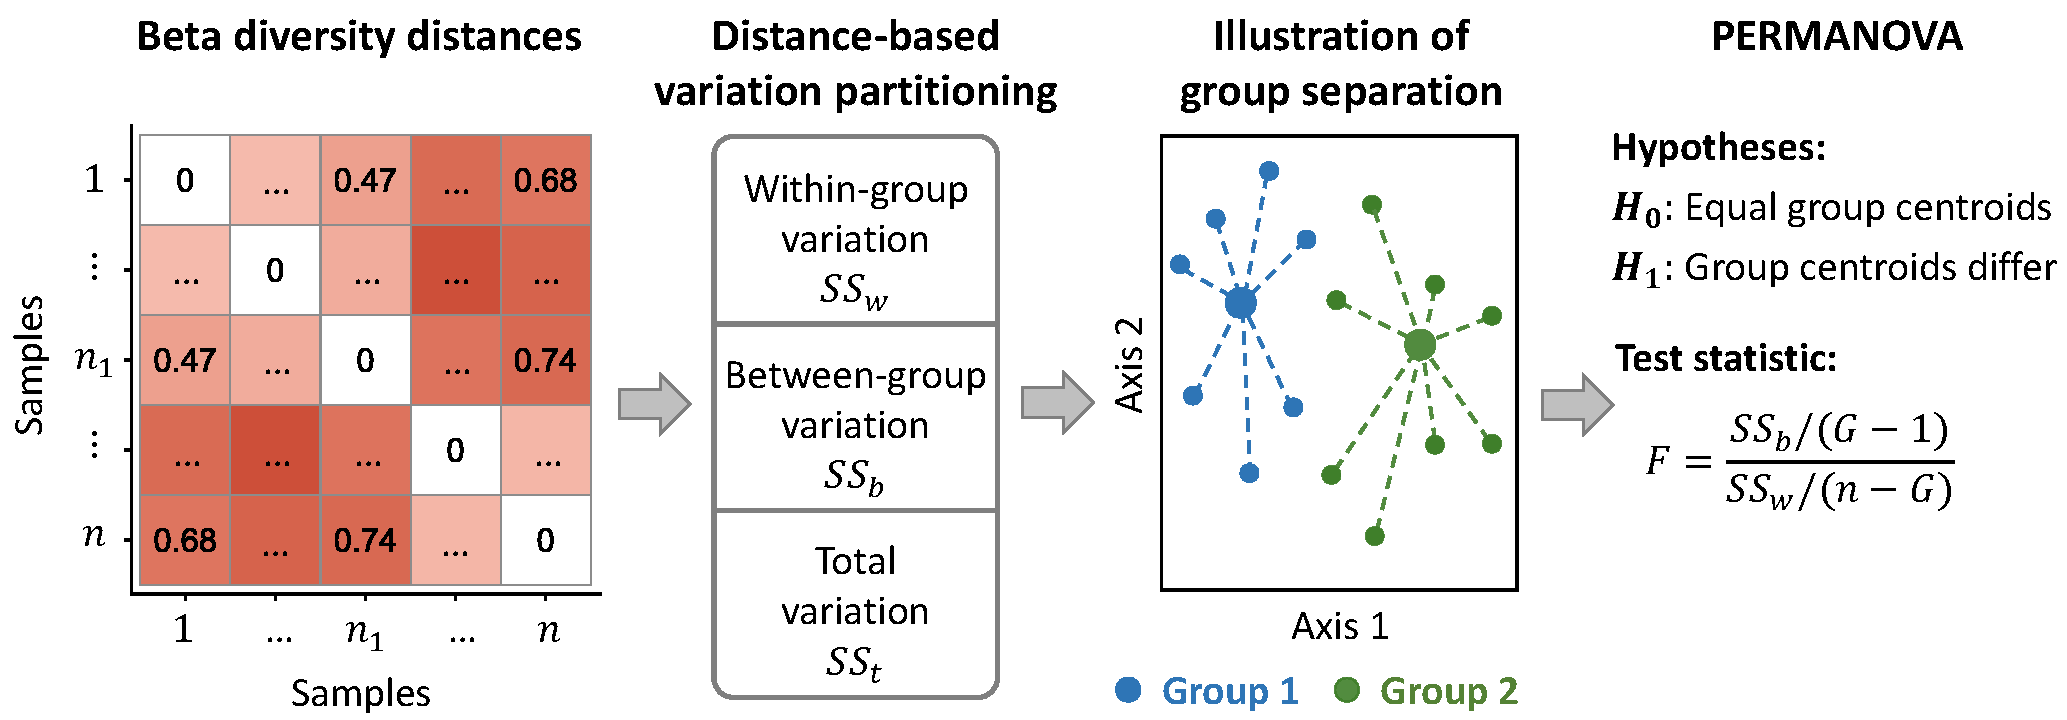
\includegraphics[width=\textwidth]{../ch03_community_level/overview_figures/overview_PERMANOVA.pdf}
	\caption{\textbf{Overview of PERMANOVA for between-sample diversity analysis.} A sample-by-sample beta-diversity distance matrix is used to partition total variation into between-group and within-group components. The resulting pseudo-$F$ statistic compares the relative magnitude of between-group to within-group variation and is evaluated by permutation of group labels. The ordination panel provides a two-dimensional illustration of group separation; PERMANOVA itself uses the full distance-based representation rather than only the displayed axes.}
	\label{fig:3community:overview_permanova}
\end{figure}


Ordination provides a visual summary of between-sample dissimilarities, but formal assessment of group differences requires statistical testing. Figure~\ref{fig:3community:overview_permanova} summarizes the main idea of permutational multivariate analysis of variance (PERMANOVA): a beta-diversity distance matrix is decomposed into within-group and between-group variation, and the resulting pseudo-$F$ statistic is evaluated against a permutation-based null distribution. PERMANOVA was originally proposed by \citet{anderson2001new} and is widely used for distance-based inference in ecological community analysis \citep{anderson2013permanova,legendre2012numerical}. It is commonly interpreted as testing whether predefined groups differ in their centroids within the multivariate representation induced by a chosen dissimilarity measure.

Several distance-based tests have been proposed for ecological community data, including analysis of similarities (ANOSIM) \citep{clarke1993nonparametric}, the Mantel test \citep{mantel1967detection}, multi-response permutation procedures \citep{mielke2001permutation}, and PERMANOVA \citep{anderson2001new}. These methods differ in the hypotheses they target and in their sensitivity to the structure of the distance matrix. 
PERMANOVA is widely used in microbiome studies because it can accommodate a broad class of dissimilarity measures, continuous and categorical covariates, and multi-factor study designs through a regression-type model formula \citep{kers2022power}. In contrast to purely rank-based or pairwise procedures, PERMANOVA partitions variation in the distance matrix into components attributable to explanatory variables and residual variation, yielding an $R^2$-type effect size in addition to a permutation-based $p$-value. For Euclidean distances, the group centroids correspond to arithmetic means of the sample coordinates. For general dissimilarities, the same idea is formulated through the distance-based representation underlying the sums-of-squares decomposition.

Let $\mathbf{D}=(d_{kl})$ denote the dissimilarity matrix between $n$ samples, and let $g_k\in\{1,\ldots,G\}$ denote the group assignment of sample $k$. PERMANOVA expresses the total variation represented by the dissimilarity matrix as a sum of squares and partitions this variation into between-group and within-group components \citep{anderson2001new}. In the one-way case, this yields a pseudo-$F$ statistic of the form
\begin{equation}
F_{\mathrm{PERM}}=\frac{\mathrm{SS}_{\mathrm{b}}/(G-1)}{\mathrm{SS}_{\mathrm{w}}/(n-G)},
\end{equation}
where $\mathrm{SS}_{\mathrm{b}}$ denotes the variation explained by differences between group centroids and $\mathrm{SS}_{\mathrm{w}}$ denotes the residual within-group variation. For more general models, the same principle can be extended by partitioning sums of squares according to explanatory variables, analogous to the analysis of variance for univariate responses \citep{mcardle2001fitting,anderson2001new}.

Because the sampling distribution of $F_{\mathrm{PERM}}$ is generally not available analytically, significance is assessed by permutation. Under the null hypothesis of no association between community composition and the variable of interest, the sample labels are exchangeable according to the chosen permutation scheme. The pseudo-$F$ statistic is recomputed for permuted label assignments, and the observed statistic is compared with the resulting permutation distribution. The empirical permutation $p$-value is then obtained as
\begin{equation}
p_{\mathrm{emp}}=\frac{1+\sum_{b=1}^B I(F_b^\ast\geq F_{\mathrm{obs}})}{1+B},
\end{equation}
where $F_{\mathrm{obs}}$ denotes the observed pseudo-$F$ statistic and $F_b^\ast$ the statistic obtained from the $b$-th permutation. The addition of one to numerator and denominator avoids zero permutation $p$-values and corresponds to the convention discussed in Chapter~\ref{ch:permapprox}.

The interpretation of PERMANOVA depends on the dissimilarity measure used as input. Applying PERMANOVA to Bray--Curtis dissimilarities tests for a group effect in the distance-based representation of relative abundance profiles. Applying it to Aitchison distances tests for group differences in the corresponding log-ratio representation. In sparse microbiome data, this interpretation is conditional on the preprocessing used before CLR transformation, including filtering, normalization to a common compositional scale, and zero replacement. Thus, PERMANOVA does not test a universal notion of ``community difference'', but a difference defined by the geometry induced by the selected distance measure. This is important because different distances emphasize different aspects of the data, as discussed in the previous subsections.

A well-known limitation of PERMANOVA is that significant results may reflect differences in group centroids, differences in within-group dispersion, or a combination of both \citep{anderson2006distance,warton2012distance}. In univariate terms, this is analogous to the difficulty of distinguishing a difference in means from a difference in variances when both affect the test statistic. PERMANOVA results should therefore be interpreted together with ordination plots and, where relevant, with tests for homogeneity of multivariate dispersion such as PERMDISP \citep{anderson2006distance}. This is particularly important in unbalanced designs, where heterogeneity of dispersion can affect type I error and interpretation \citep{anderson2013permanova}. This motivates the explicit assessment of community dispersion in the following subsection.

In R, PERMANOVA is widely applied using the \texttt{adonis2} function from the \texttt{vegan} package \citep{oksanen2024vegan}. The \texttt{adonis2} implementation supports formula-based models, different types of sums of squares, and restricted permutation schemes, making it suitable for ecological and microbiome study designs. Computationally efficient implementations such as \texttt{fast.adonis} have been proposed for larger microbiome data sets and produce results consistent with \texttt{adonis} and \texttt{adonis2} for corresponding PERMANOVA quantities \citep{li2022fastadonis}. In the PASTURE application in Chapter~\ref{ch:application}, we use \texttt{adonis2} because \texttt{fast.adonis} is not needed due to the low dimensionality of the data. The analysis is performed for both beta-diversity representations introduced above, namely Bray--Curtis dissimilarities on relative abundance profiles and Aitchison distances after normalization, multiplicative replacement, and CLR transformation. Since PERMANOVA relies on permutation-based inference, we additionally use the \texttt{permApprox} workflow introduced in Chapter~\ref{ch:permapprox} to assess whether the resulting permutation $p$-values can be refined by tail approximation.


%====================================
\subsection{Community dispersion}
\label{sec:3community:between:dispersion}
%====================================

The between-sample dissimilarities introduced above can be used not only to assess differences between groups, but also to quantify heterogeneity within groups. While PERMANOVA focuses on differences between group centroids in the space induced by a dissimilarity measure, community dispersion describes how strongly samples vary around their corresponding group centroid. It can therefore be interpreted as a multivariate analogue of within-group variance \citep{anderson2006distance}.

Let $\mathbf{D}=(d_{kl})$ denote a dissimilarity matrix between samples and let $g_k\in\{1,\ldots,G\}$ denote the group assignment of sample $k$. For a group $g$, let $\mathbf{z}_k$ denote the coordinate representation of sample $k$ obtained from the chosen dissimilarity matrix, for example through principal coordinates analysis. The group centroid is then given by the average coordinate vector
\begin{equation}
	\bar{\mathbf{z}}_g=\frac{1}{n_g}\sum_{k:g_k=g} \mathbf{z}_k.
\end{equation}
The dispersion of sample $k$ is defined as its distance to the centroid of its group in this coordinate representation,
\begin{equation}
	\delta_k=\left\|\mathbf{z}_k-\bar{\mathbf{z}}_{g_k}\right\|_2.
\end{equation}
where $n_g$ denotes the number of samples in group $g$. Larger values of $\Delta_g$ indicate greater within-group heterogeneity in microbial community composition, whereas smaller values indicate that samples within the group are more similar to each other.

For Euclidean distances, such as the Aitchison distance, the centroid corresponds to the arithmetic mean of the transformed sample coordinates within the group. For non-Euclidean dissimilarities, such as Bray--Curtis dissimilarity, the same idea is implemented through a coordinate representation, typically principal coordinates analysis. In that case, distances to group centroids or spatial medians are computed in the coordinate space that represents the original dissimilarities as closely as possible \citep{anderson2006distance}. Consequently, dispersion estimates should always be interpreted relative to the chosen dissimilarity measure and data representation.

Differences in community dispersion can be assessed using distance-based tests for homogeneity of multivariate dispersions, commonly referred to as PERMDISP \citep{anderson2006distance}. The corresponding null hypothesis is
\begin{equation}
H_0:\Delta_1=\Delta_2=\cdots=\Delta_G.
\end{equation}
In practice, the sample-wise distances $\delta_k$ are treated as univariate responses and compared between groups using an analysis-of-variance type statistic. Significance is commonly assessed using permutation-based procedures. In R, this approach is implemented in the \texttt{betadisper} function of the \texttt{vegan} package, with permutation-based testing available through \texttt{permutest.betadisper} \citep{oksanen2024vegan}.

Community dispersion captures a different aspect of group structure than centroid location. A group with larger dispersion does not necessarily have a different average community composition, but may exhibit greater between-individual variability. In microbiome studies, increased dispersion indicates greater between-individual heterogeneity in community composition and may be consistent with less stable community structures. At the same time, dispersion is important for the interpretation of PERMANOVA: if groups differ in their within-group dispersion, a significant PERMANOVA result may reflect heterogeneity differences rather than, or in addition to, differences in group centroids \citep{anderson2006distance,warton2012distance}. Reporting PERMDISP alongside PERMANOVA therefore helps assess whether differences in within-group dispersion accompany a PERMANOVA finding and supports a more careful interpretation of distance-based microbiome comparisons.

In the PASTURE application in Chapter~\ref{ch:application}, community dispersion is assessed for the same beta-diversity representations used in PERMANOVA, namely Bray--Curtis dissimilarities on relative abundance profiles and Aitchison distances after normalization, multiplicative replacement, and CLR transformation. This allows within-group heterogeneity to be compared on both the ecological relative-abundance scale and the log-ratio scale. Since PERMDISP is also commonly assessed by permutation, we additionally evaluate whether the resulting permutation $p$-values can be refined using the \texttt{permApprox} workflow introduced in Chapter~\ref{ch:permapprox}.

%%%%%%%%%%%%%%%%%%%%%%%%%%%%%%%%%%%%%
\section{Regression models for compositional responses}
\label{sec:3community:regression}
%%%%%%%%%%%%%%%%%%%%%%%%%%%%%%%%%%%%%

\begin{figure}[!ht]
\centering
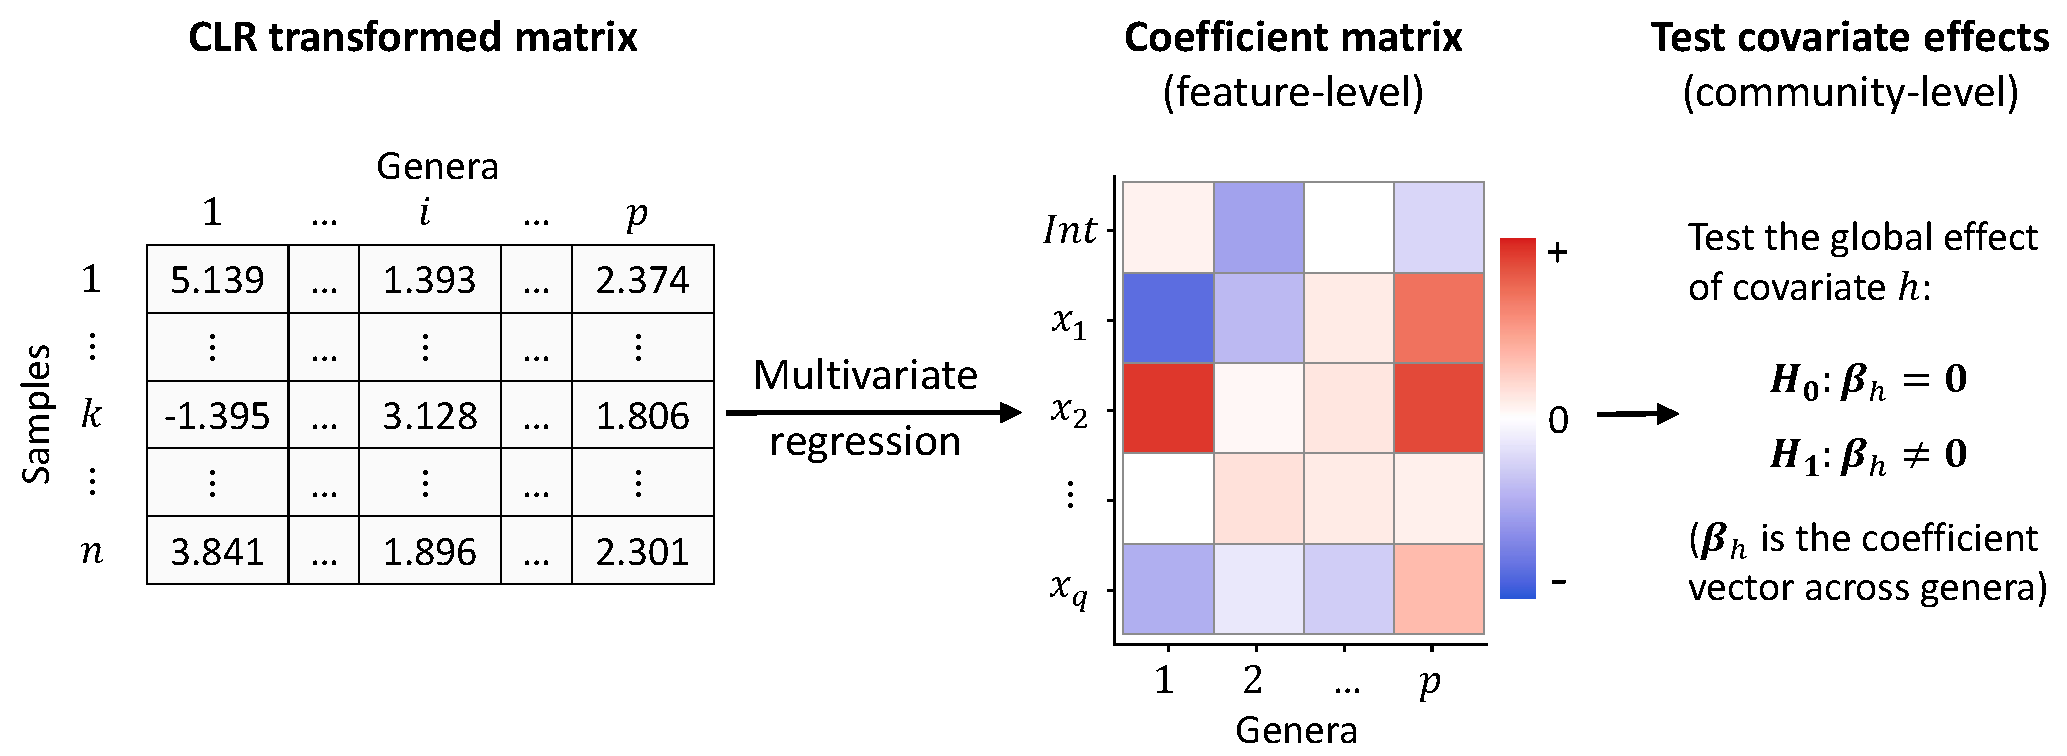
\includegraphics[width=\textwidth]{../ch03_community_level/overview_figures/overview_regression.pdf}
\caption{\textbf{Overview of CLR-based multivariate regression.} A CLR-transformed microbiome count matrix is modeled jointly as a multivariate response using sample-level covariates. The fitted model yields a coefficient matrix with one coefficient vector across taxa for each covariate. Community-level inference tests whether the coefficient vector associated with covariate $h$ is equal to the zero vector, corresponding to no association between that covariate and the overall microbial composition.}
\label{fig:community:regression:overview}
\end{figure}

Regression models provide a model-based perspective on community-level microbiome analysis. Instead of summarizing each sample by a single diversity value or representing between-sample differences only through a dissimilarity matrix, the microbial profile itself can be treated as a multivariate response. This makes it possible to ask whether sample-level covariates are associated with systematic shifts in the microbial composition as a whole. In the context of this thesis, such models are used as global community-level analyses: the main inferential target is not a single taxon-specific coefficient, but the joint covariate effect across the transformed microbial profile.

Figure~\ref{fig:community:regression:overview} summarizes this regression perspective. The following subsections first place the approach in the broader landscape of models for microbial compositions and then introduce the CLR-based multivariate regression model used in this thesis.

%====================================
\subsection{Approaches for modeling microbial compositions}
\label{sec:3community:regression:approaches}
%====================================

Regression models with microbial compositions as response variables can be formulated in different ways, depending on how the simplex constraint, sequencing variability, sparsity, high dimensionality, and covariance between taxa are represented. A first class of approaches models the composition directly by using distributions defined on the simplex. Dirichlet regression is a classical example and provides a generalized linear model-type framework for compositional responses \citep{maier2014dirichletreg}. Such models respect the constant-sum constraint by construction, but the Dirichlet distribution imposes a restrictive mean--variance relationship and negative dependence structure, which can be limiting for sparse and overdispersed microbiome data.

\newpage
A second class of approaches models the observed count vector while introducing a latent compositional layer. Logistic-normal multinomial regression, for example, combines multinomial sampling of sequencing counts with latent log-ratio variables whose mean depends on sample-level covariates \citep{xia2013logistic}. This is attractive for microbiome data because it can represent sampling variability, overdispersion, sampling zeros, and a more flexible covariance structure between taxa. However, such hierarchical count models typically require stronger distributional assumptions and more involved estimation than transformation-based approaches.

A third approach is to transform the microbial composition into log-ratio coordinates and then use regression ideas in the transformed space. This strategy is closely aligned with compositional data analysis, where log-ratio transformations are used to represent relative information in Euclidean coordinates \citep{aitchison1986statistical,gloor2017microbiome,quinn2019field}. Related microbiome methods include linear models on centered log-ratio transformed taxa, as used for example in LinDA for differential abundance analysis \citep{zhou2022linda}, and the LDM-clr framework, which extends the linear decomposition model \citep{hu2020testing} to centered-log-ratio-transformed microbiome data and provides both global and taxon-level tests \citep{hu2023compositional}.

In genuinely high-dimensional microbiome settings with $p\gg n$, unrestricted multivariate regression models are usually not appropriate without additional structural assumptions. The coefficient matrix then contains many parameters relative to the available sample size, and classical multivariate inference may require covariance matrices that are singular or unstable. A common strategy is therefore to impose low-rank, sparse, or latent-factor structure on the multivariate response model. Multivariate reduced-rank regression \citep{reinsel2022multivariate} assumes that the coefficient matrix has low rank, so that covariate effects on many taxa are represented through a smaller number of latent response directions. Sparse reduced-rank regression further combines this low-dimensional structure with sparsity, allowing only selected covariates or response coordinates to contribute to the dominant association patterns. For microbiome count data, count-based variants are particularly relevant because they can account for overdispersion and discreteness directly. For example, \citet{mishra2022negative} proposed negative-binomial reduced-rank regression and negative-binomial co-sparse factor regression to jointly model overdispersed amplicon sequencing counts using low-rank or sparse factor structure. More generally, latent factor models and regularized multivariate regression models provide a principled way to address high-dimensional, sparse, and dependent microbial responses. These approaches address an additional aspect of the regression problem compared with the transformation-based regression considered below: they regularize or factorize the high-dimensional response structure, whereas the model used in this thesis primarily addresses compositionality by working in log-ratio coordinates.

In the present chapter, we follow the transformation-based perspective, but use it as a community-level regression analysis. This interpretation is appropriate when inference focuses on joint covariate effects across the complete microbial profile rather than on separate taxon-specific coefficients, and when the response dimension remains moderate relative to the sample size after aggregation and filtering. This is the case in the PASTURE application in Section~\ref{sec:7app:regression}, where the analysis is conducted at genus level after prevalence filtering. The approach should therefore not be understood as a general solution to high-dimensional microbial response regression, but as a pragmatic model-based approach for studying covariate effects on microbial compositions in moderate-dimensional settings.

%====================================
\subsection{CLR-based multivariate regression}
\label{sec:3community:regression:clr_model}
%====================================

Following the general strategy introduced in Chapter~\ref{ch:microbiome}, we use a CLR-based representation when the microbial composition enters the model as a multivariate response. This avoids formulating regression models directly on raw counts or untransformed relative abundances, whose components carry relative rather than absolute information and may be affected by closure-induced dependencies and library size variation \citep{aitchison1986statistical,gloor2017microbiome,quinn2019field}. 

Using a CLR transformation raises again the question of zero handling. In this regression setting, the transformed taxon profiles are the response variables, so artificial changes in their marginal distributions can directly affect coefficient estimation and testing. Following the preprocessing strategy described in Section~\ref{sec:2micro:preprocessing_choices_thesis}, count data are first brought to a common compositional scale before zero replacement. We then use multiplicative replacement followed by the standard CLR transformation, unless a method-specific alternative is explicitly required. Multiplicative replacement yields strictly positive compositions while preserving ratios among originally non-zero components. This is preferable here to global offset addition, which changes ratios among observed components and can therefore alter the transformed response values before the regression model is fitted. 
Let $\mathbf{x}_k^\ast$ denote the normalized and multiplicatively replaced composition obtained from sample $\mathbf{x}_k$, and define
\begin{equation}
\mathbf{y}_k=\operatorname{CLR}\left(\mathbf{x}_k^\ast\right)\in\mathbb{R}^p
\end{equation}
as the CLR-transformed microbial profile of sample $k$. A multivariate regression model for the transformed composition can then be written as
\begin{equation}
\mathbf{y}_k = \boldsymbol{\beta}_0 + \sum_{h=1}^q w_{kh}\boldsymbol{\beta}_h + \boldsymbol{\varepsilon}_k,
\end{equation}
where $\mathbf{w}_k=(w_{k1},\ldots,w_{kq})^\top$ denotes the vector of $q$ sample-level covariates for sample $k$, $\boldsymbol{\beta}_0\in\mathbb{R}^p$ is an intercept vector, $\boldsymbol{\beta}_h\in\mathbb{R}^p$ denotes the multivariate effect of covariate $h$ across the CLR coordinates, and $\boldsymbol{\varepsilon}_k\in\mathbb{R}^p$ denotes the residual vector. Equivalently, the coefficient vectors can be collected in the coefficient matrix $\mathbf{B}=(\boldsymbol{\beta}_1,\ldots,\boldsymbol{\beta}_q)^\top\in\mathbb{R}^{q\times p}$, yielding the compact representation
\begin{equation}
\mathbf{y}_k = \boldsymbol{\beta}_0 + \mathbf{B}^\top \mathbf{w}_k + \boldsymbol{\varepsilon}_k.
\end{equation}
In this representation, row $h$ of $\mathbf{B}$ contains the coefficients describing the effect of covariate $h$ across all CLR coordinates, whereas column $i$ contains the coefficients associated with CLR coordinate $i$ across all covariates. 

The coefficient interpretation follows the CLR scale on which the response is modeled. A positive coefficient for CLR coordinate $i$ indicates that, conditional on the other covariates, taxon $i$ tends to increase relative to the sample-wise geometric mean as the corresponding covariate increases. Since CLR coordinates express each taxon relative to the sample-wise geometric mean, coefficients describe changes in the relative position of taxa within the microbial composition. They should therefore be understood as effects on the log-ratio representation of the community rather than as marginal effects on absolute or raw relative abundances. 

For the purposes of this chapter, the main inferential target is not an individual coefficient but the covariate-specific effect vector $\boldsymbol{\beta}_h$. Testing whether $\boldsymbol{\beta}_h=\mathbf{0}$ asks whether covariate $h$ is associated with the microbial composition as a whole. This distinguishes compositional-response regression from feature-level regression, where the primary focus lies on taxon-specific effects. At the same time, inference for the coefficient matrix $\mathbf{B}$ is non-trivial because microbiome data are high-dimensional and the CLR coordinates are statistically dependent. The question of how covariate effects are tested is therefore considered separately in the next subsection.

%====================================
\subsection{Testing covariate effects}
\label{sec:3community:regression:testing}
%====================================

In compositional-response regression, the main inferential question is whether a sample-level covariate is associated with the microbial composition as a whole. For covariate $h$, this corresponds to the global null hypothesis
\begin{equation}
H_0:\boldsymbol{\beta}_h=\mathbf{0},
\end{equation}
where $\boldsymbol{\beta}_h\in\mathbb{R}^p$ denotes the vector of coefficients for covariate $h$ across all CLR coordinates. Rejecting this null hypothesis indicates that the covariate is associated with a multivariate shift in the transformed microbial composition. The test is therefore community-level in its interpretation, even though the coefficient vector contains taxon-specific components.

Classical multivariate linear models are commonly tested using MANOVA-type statistics, such as Wilks' lambda, Pillai's trace, the Hotelling--Lawley trace, or Roy's largest root \citep{rencher2002methods}. These statistics compare the variation explained by a covariate with the residual variation in the multivariate response. In matrix notation, let $\mathbf{Y}\in\mathbb{R}^{n\times p}$ denote the matrix of CLR-transformed microbial profiles and let $\mathbf{W}\in\mathbb{R}^{n\times q}$ denote the design matrix of sample-level covariates. Testing a covariate can be formulated by comparing a full model including the covariate with a reduced model in which the covariate is omitted. The difference in fitted values or residual sums of squares then quantifies the contribution of that covariate to explaining variation in the transformed microbial composition.

However, the assumptions underlying classical MANOVA are often difficult to justify for microbiome data. The CLR coordinates are statistically dependent because they are constrained to sum to zero, and microbiome data are typically sparse and high-dimensional, with the number of taxa often comparable to or larger than the number of samples \citep{aitchison1986statistical,gloor2017microbiome,xia2024applied}. For CLR-transformed responses, the residual covariance matrix is structurally singular because the coordinates sum to zero. High dimensionality can further make covariance estimation unstable, and normality assumptions for transformed microbial profiles are at best approximate. Classical asymptotic MANOVA approximations should therefore be interpreted with caution in microbiome applications, especially when $p$ is not small relative to $n$ \citep{chen2010twosample}.

A permutation-based alternative is to use a global test statistic for the covariate effect and approximate its null distribution under an appropriate exchangeability scheme \citep{freedman1983nonstochastic,winkler2014permutation}. Related microbiome-specific approaches include the linear decomposition model and its CLR-based extension, which use regression-type formulations to obtain community-level tests together with taxon-level information \citep{hu2020testing,hu2023compositional}. One possible statistic is the reduction in multivariate residual sum of squares when covariate $h$ is added to the model,
\begin{equation}
t_h=\mathrm{RSS}_{\mathrm{red},h}-\mathrm{RSS}_{\mathrm{full}},
\end{equation}
where the residual sum of squares is computed over all samples and CLR coordinates, for example as the squared Frobenius norm of the residual matrix,
\begin{equation}
\mathrm{RSS}=\|\mathbf{Y}-\widehat{\mathbf{Y}}\|_F^2.
\end{equation}
Here, $\mathrm{RSS}_{\mathrm{full}}$ denotes the residual sum of squares of the full multivariate model and $\mathrm{RSS}_{\mathrm{red},h}$ denotes the residual sum of squares of the model without covariate $h$. Larger values of $t_h$ indicate that the covariate explains more variation in the CLR-transformed microbial profile. This construction is analogous to comparing nested regression models, but the null distribution is obtained empirically rather than from a parametric approximation.

The empirical permutation $p$-value is then computed by comparing the observed statistic $t_{h,\mathrm{obs}}$ with the statistics $t_{hb}^\ast$, $b=1,\ldots,B$, obtained from permuted data:
\begin{equation}
p_{\mathrm{emp},h}=\frac{1+\sum_{b=1}^B I(t_{hb}^\ast\geq t_{h,\mathrm{obs}})}{1+B}.
\end{equation}
This formulation follows the general permutation-testing principle discussed in Chapter~\ref{ch:permapprox}. It is attractive in the present setting because it avoids relying on a parametric null distribution for a high-dimensional multivariate response and can be applied with the same transformed response matrix used for coefficient estimation.

In the PASTURE application in Chapter~\ref{ch:application}, compositional-response regression is used as an additional community-level analysis for the selected birth-related covariates. The focus is on the global covariate tests $H_0:\boldsymbol{\beta}_h=\mathbf{0}$, not on interpreting individual taxon-specific coefficients as separate feature-level findings. Since the tests are permutation-based, we also evaluate whether the resulting permutation $p$-values can be refined using the \texttt{permApprox} workflow introduced in Chapter~\ref{ch:permapprox}. This allows the regression-based analysis to be compared with the distance-based PERMANOVA results while retaining the same inferential framework for limited permutation settings.


%%%%%%%%%%%%%%%%%%%%%%%%%%%%%%%%%%%%%
\section{Compositional equivalence}
\label{sec:3community:compositional_equivalence}
%%%%%%%%%%%%%%%%%%%%%%%%%%%%%%%%%%%%%

\begin{figure}[H]
	\centering
	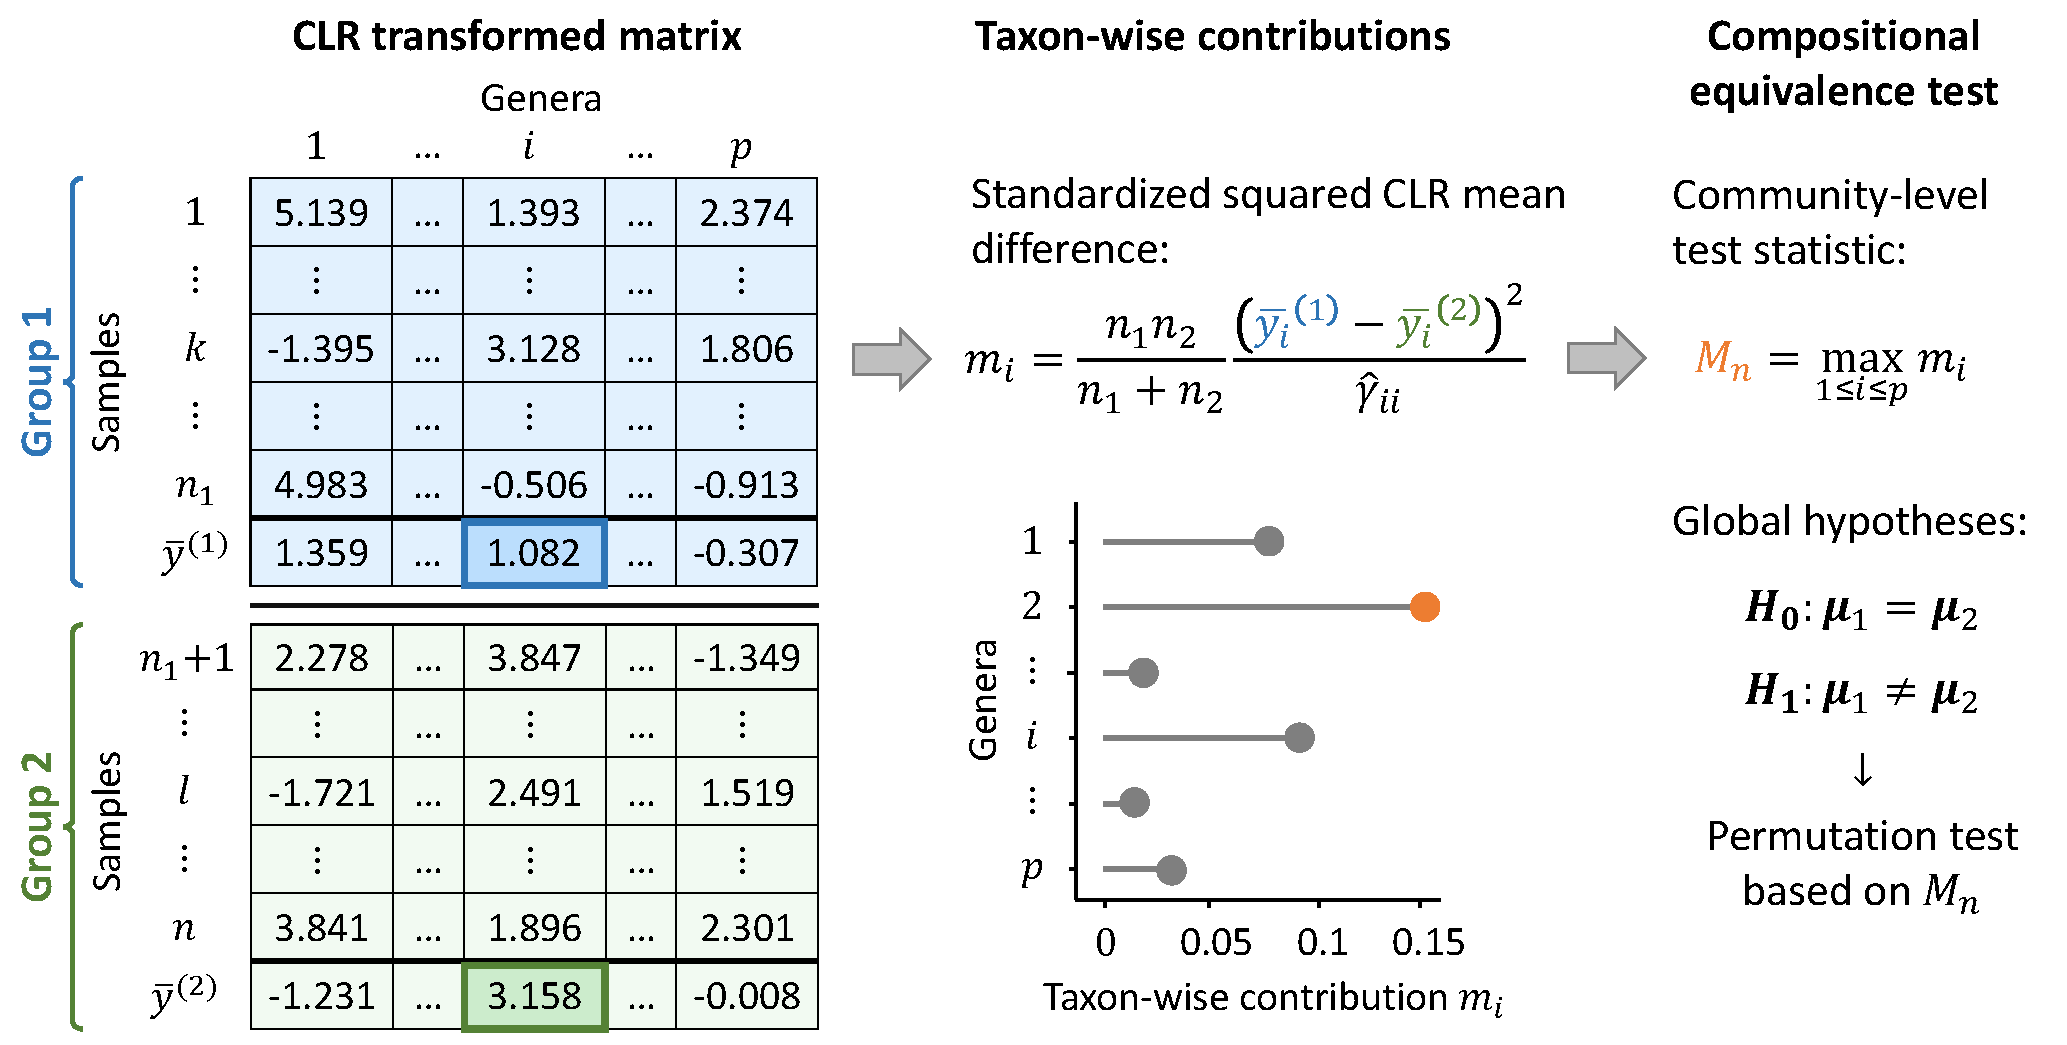
\includegraphics[width=\textwidth]{../ch03_community_level/overview_figures/overview_comp_equivalence.pdf}
	\caption{\textbf{Overview of compositional equivalence testing.} The microbiome data are represented on the CLR scale, and group-specific mean CLR vectors are computed for the two groups. For each taxon, the standardized squared difference between the group means defines a taxon-wise contribution $m_i$. The largest contribution is summarized by the maximum-type statistic $M_n$, which is evaluated using a permutation test of equality between the group mean CLR compositions.}
	\label{fig:3community:overview_comp_equivalence}
\end{figure}

The preceding sections considered community-level summaries from complementary perspectives. Within-sample diversity reduces each microbial profile to a scalar summary, between-sample dissimilarity represents community structure through pairwise distances between samples, and regression models for compositional responses treat the transformed microbial profile as a multivariate outcome. \emph{Compositional equivalence} provides a further perspective at the boundary between community-level and feature-level inference. It is constructed from taxon-specific differences in centered log-ratio coordinates, but these differences are aggregated through a maximum-type statistic, yielding a single global test for the microbial composition. The main steps of the procedure are summarized in Figure~\ref{fig:3community:overview_comp_equivalence}.

%====================================
\subsection{Concept and hypothesis}
\label{sec:3community:comp_equivalence:concept}
%====================================

The idea of compositional equivalence is to compare the average microbial composition between groups while respecting that the observed data contain only relative abundance information. A direct comparison of raw mean count vectors or mean relative abundance vectors would not define an appropriate inferential target, because such comparisons are affected by library size differences and the closure constraint discussed in Chapter~2. Following the compositional data framework, \citet{cao2018twosample} formulate group comparison in log-ratio coordinates. In this thesis, compositional equivalence is computed after total sum normalization, multiplicative replacement of zero counts, and CLR transformation, following the preprocessing strategy described in Section~\ref{sec:2micro:preprocessing_choices_thesis}. The CLR transformation itself was introduced in Section~\ref{sec:2micro:norm:log-ratios}, and its use in the presence of zeros was discussed in Section~\ref{sec:2micro:clr_with_zeros}. Let $\mathbf{y}_k^{(g)}$ denote the resulting CLR representation of the microbial composition of sample $k$ in group $g\in\{1,2\}$. Group differences can then be formulated as differences between the corresponding mean CLR vectors.

The null hypothesis states that the two groups have equal mean log-ratio composition,
\begin{equation}
H_0:\boldsymbol{\mu}_1=\boldsymbol{\mu}_2,
\end{equation}
where $\boldsymbol{\mu}_g=\mathbb{E}\left(\mathbf{y}_k^{(g)}\right)$ denotes the population mean of the CLR-transformed composition in group $g$. Since CLR coordinates are invariant to multiplication of the original composition by a positive constant, this hypothesis is formulated in terms of relative microbial composition rather than absolute microbial load. Thus, compositional equivalence is a global statement about equality of mean relative composition in log-ratio space. Deviations from this null hypothesis indicate that the groups differ in at least one component of their mean CLR composition, but not necessarily that they differ in total microbial load, which is not identified from standard sequencing data.

%====================================
\subsection{Maximum-type test statistic}
\label{sec:3community:comp_equivalence:statistic}
%====================================

A natural test statistic for this hypothesis compares the sample mean vectors in CLR space. Let
\begin{equation}
	\bar{\mathbf{y}}^{(g)} = 
	\frac{1}{n_g}
	\sum_{k=1}^{n_g}
	\mathbf{y}_k^{(g)}
\end{equation}
denote the sample mean CLR vector in group $g$, and let $\hat{\gamma}_{ii}$ denote the pooled within-group variance estimate of CLR coordinate $i$. For each taxon $i$, the standardized squared difference between the group-specific sample means is defined as
\begin{equation}
	m_i = \frac{n_1n_2}{n_1+n_2} \frac{\left(\bar{y}_i^{(1)}-\bar{y}_i^{(2)}\right)^2}
	{\hat{\gamma}_{ii}}.
	\label{eq:3community:comp_equivalence:coordinate_contribution}
\end{equation}
The statistic proposed by \citet{cao2018twosample} is then obtained by taking the maximum over all coordinate-wise contributions,
\begin{equation}
	M_n = \max_{1\leq i\leq p} m_i.
	\label{eq:3community:comp_equivalence:maximum_statistic}
\end{equation}
Thus, the procedure evaluates standardized differences between group-specific CLR means for all taxa and summarizes the largest contribution in a single global statistic. This maximum-type construction is motivated by sparse alternatives, in which differences between groups are concentrated in only a small number of taxa. In such settings, statistics that aggregate contributions across many coordinates may dilute the signal, whereas a maximum statistic is sensitive to the largest standardized deviation. Nevertheless, the inferential target remains global: the test assesses whether the mean CLR compositions differ between groups, rather than identifying individual taxa responsible for a potential difference.


%====================================
\subsection{Permutation-based inference and application}
\label{sec:3community:comp_equivalence:permutation}
%====================================

In microbiome applications, randomization-based inference provides an attractive alternative to asymptotic approximations. \citet{sommer2022randomizationbased} considered a related maximum-type test within a randomization-based causal-inference framework. They emphasized that, because sequencing data are compositional, a change in the observed abundance of one taxon necessarily affects the observed counts of other taxa, even when these taxa have no causal role. Their approach therefore applies a CLR transformation before comparing group-specific mean log-ratio compositions and uses a maximum-type statistic based on standardized differences between group mean CLR coordinates.

In this thesis, $M_n$ is used as a permutation test statistic rather than being evaluated through an asymptotic approximation. Since total sum scaling, multiplicative zero replacement, and CLR transformation are applied sample-wise and independently of the group labels, the transformed data are kept fixed during the permutation procedure. Group labels are then permuted repeatedly, and the statistic $M_n^\ast$ is recomputed for each permuted labeling, including the corresponding group-specific mean vectors and pooled within-group coordinate variances. The observed statistic is compared with the resulting permutation distribution. For $B$ permutations, the empirical permutation $p$-value is computed as
\begin{equation}
	p_{\mathrm{emp}} = \frac{1+\sum_{b=1}^{B} I\left(M_{n,b}^\ast \geq M_n\right)} {B+1}.
	\label{eq:3community:comp_equivalence:empirical_pvalue}
\end{equation}
This procedure is valid when samples are exchangeable with respect to the group labels under the null hypothesis. More complex study designs may require restricted or covariate-adjusted permutation schemes.

The permutation-based formulation is aligned with the general inferential strategy of this thesis and avoids reliance on large-sample approximations whose accuracy may be difficult to assess for sparse, high-dimensional microbiome data. At the same time, it inherits the finite-resolution limitation of permutation testing: with a limited number of permutations, attainable $p$-values lie on a discrete grid. Small empirical $p$-values from the maximum-type test are therefore refined using the \texttt{permApprox} framework developed in Chapter~\ref{ch:permapprox}. In this setting, $M_n$ is treated as the observed right-tailed test statistic, and the permuted values $M_{n,1}^\ast,\ldots,M_{n,B}^\ast$ define the permutation distribution used for tail approximation.

Within the organization of this thesis, compositional equivalence serves as a final community-level comparison that is close to feature-level inference. In contrast to within-sample diversity analysis, it uses the complete transformed microbial profile rather than reducing each sample to a scalar ecological summary. In contrast to PERMANOVA, it is not based on pairwise sample dissimilarities, but on differences between group-specific mean CLR vectors. In contrast to feature-level differential abundance analysis, it does not yield one hypothesis test per taxon, but combines taxon-wise CLR contrasts into a single global test. In the PASTURE application, this makes the method a useful additional analysis for selected two-group contrasts identified in the preceding community-level analyses.

A significant result indicates evidence that the groups differ in their mean log-ratio composition, with particular sensitivity to sparse shifts in CLR coordinates. It does not, by itself, identify the taxa responsible for the difference and does not imply a difference in absolute microbial load. Conversely, a non-significant result should be interpreted as a lack of evidence against equality of mean CLR compositions under the chosen preprocessing strategy and test statistic, rather than as proof of identical microbial communities.

% !TeX root = ../thesis.tex

%%%%%%%%%%%%%%%%%%%%%%%%%%%%%%%%%%%%%%%%%%
\thesischapter[ch:feature]
  {``Why are there so many kinds of animals?''}
  {--- G. Evelyn Hutchinson, 1959}
  {Feature-level measures}
\nocite{hutchinson1959homage}
\chapterabstract{This chapter turns from aggregated community summaries to the analysis of individual microbial features. It distinguishes exploratory taxon-level analysis from comparative feature-level inference, where the aim is to identify taxa whose abundance or distribution differs between groups. Particular attention is given to the statistical complications caused by compositionality, sparsity, and heterogeneous library sizes. The chapter reviews common methodological approaches to differential abundance and differential distribution analysis and presents DACOMP and \texttt{waddR} as two permutation-based methods that are later combined with the \texttt{permApprox} framework to improve p-value resolution under limited permutation budgets.}
\chaptercontents

%%%%%%%%%%%%%%%%%%%%%%%%%%%%%%%%%%%%%%%%%%

%%%%%%%%%%%%%%%%%%%%%%%%%%%%%%%%%%%%%
\section{Introduction}
\label{sec:feature:intro}
%%%%%%%%%%%%%%%%%%%%%%%%%%%%%%%%%%%%%

Feature-level analysis investigates microbial taxa individually rather than through aggregated community summaries or network structures. Given a microbiome count matrix $X \in \mathbb{N}_0^{n \times p}$, the aim is to characterize or compare single features across samples, groups, or covariate patterns. This perspective provides a higher taxonomic resolution than community-level summaries because observed effects can be attributed to individual taxa. At the same time, it introduces additional statistical challenges, since feature-level analyses typically involve sparse, high-dimensional data and large numbers of simultaneous hypothesis tests.

Feature-related methods cover several related but distinct analysis tasks. In exploratory analyses, feature-level summaries are used to describe abundance, prevalence, and taxonomic patterns within a cohort. In comparative analyses, the objective is often to identify taxa whose abundance differs between groups, which is commonly referred to as differential abundance analysis. However, group differences may also involve changes in variability, zero structure, or distributional shape rather than shifts in abundance level alone. This motivates differential distribution analysis, where the full feature-specific distribution is compared across groups. A further class of feature-related methods uses microbial taxa as explanatory variables in regression or prediction models for sample-level outcomes. Such models also yield taxon-specific coefficients and therefore have a feature-level interpretation, but they address a different scientific question: whether the microbiome predicts or explains an external outcome.

In this thesis, we focus on differential abundance and differential distribution analysis. This choice reflects the aim of the application chapter, where early-life and birth-related variables are used to compare microbial profiles rather than to predict sample-specific outcomes from the microbiome. Regression models with microbial features as covariates would therefore reverse the direction of the main question. For example, they would ask whether the early microbiome predicts variables such as body mass index or other host characteristics, which is not the objective of the PASTURE analysis considered here. They are therefore acknowledged as part of the broader feature-level toolbox, but not developed further in this chapter.

The methodological focus on differential abundance and differential distribution analysis also serves a second purpose. Both approaches considered in detail in this chapter rely on permutation-based inference. DACOMP uses permutation testing for differential abundance analysis, while \texttt{waddR} uses permutation-based Wasserstein tests for differential distribution analysis. This makes both methods suitable for illustrating the finite-resolution problem of permutation p-values and for applying the \texttt{permApprox} framework developed in Chapter~\ref{ch:permapprox}. The emphasis is therefore not only on identifying taxon-specific group differences, but also on studying how permutation-based feature-level inference can be improved when only a limited number of permutations is computationally feasible.

The chapter first introduces exploratory taxon-level summaries and visualizations. It then discusses differential abundance analysis, gives an overview of common approaches, and presents DACOMP in more detail as the method used in the application chapter. Subsequently, differential distribution analysis is introduced, with a focus on the Wasserstein-based \texttt{waddR} framework and its adaptation to microbiome data. For both DACOMP and \texttt{waddR}, permutation-based inference is connected to the \texttt{permApprox} framework, which is used to refine small p-values under limited permutation budgets.

%%%%%%%%%%%%%%%%%%%%%%%%%%%%%%%%%%%%%
\section{Exploratory taxon-level analysis}
\label{sec:4feature:exploratory}
%%%%%%%%%%%%%%%%%%%%%%%%%%%%%%%%%%%%%

Exploratory feature-level analysis provides a first descriptive view of the individual microbial features observed in a microbiome study. While community-level summaries reduce each sample to diversity measures, dissimilarities, or multivariate model summaries, feature-level exploration keeps the taxonomic resolution explicit. The aim is not formal hypothesis testing, but rather to understand which features dominate the data set, how broadly they are observed across samples, and whether apparent patterns may depend on sparsity, taxonomic resolution, or a small number of highly abundant observations. Such analyses are therefore an important intermediate step between preprocessing and formal differential testing. They help to assess whether the chosen filtering, aggregation, and transformation steps are reasonable and provide context for interpreting later feature-wise results.

A basic summary at feature level is the abundance of each taxon. Depending on the analysis goal, abundance can be summarized by total read count, mean relative abundance, median relative abundance, or a transformed value such as a CLR coordinate. Total abundance highlights taxa that contribute strongly to the overall sequencing output, whereas mean or median relative abundance summarizes the relative contribution of a taxon across samples. However, these quantities can behave quite differently in sparse microbiome data. A taxon with high total abundance may occur in only a few samples, while a taxon with moderate abundance may be observed consistently across many samples. Abundance summaries should therefore usually be considered together with prevalence.

Prevalence describes the proportion of samples in which a taxon is observed, commonly defined as
\begin{equation}
\operatorname{prev}_i = \frac{1}{n}\sum_{k=1}^n I(x_{ki} > 0),
\end{equation}
where $I(\cdot)$ denotes the indicator function. Prevalence is particularly informative in sparse count matrices because it separates rare but occasionally abundant taxa from taxa that are consistently present. In practice, abundance and prevalence are often visualized jointly, for example in prevalence-abundance plots. Such plots can reveal whether the data contain a small number of highly prevalent dominant taxa, a long tail of rare taxa, or features that may be unstable targets for downstream inference. They also provide a transparent justification for prevalence- or abundance-based filtering rules.

Exploratory analyses may be performed at different taxonomic resolutions, such as ASV, genus, family, or phylum level. The choice of resolution depends on the aggregation strategy defined during preprocessing (Section~\ref{sec:2micro:aggregation}) and directly determines which features are summarized, visualized, and later tested. It is therefore important to interpret exploratory taxon-level patterns with respect to the chosen analysis unit. For example, a genus-level profile may be easier to interpret than an ASV-level profile, but it may also hide heterogeneous behavior among lower-level features that were aggregated into the same taxonomic group.

Visualization plays a central role in exploratory feature-level analysis. Stacked barplots of relative abundances provide a compact overview of dominant taxa and their variation across samples or groups. However, because only the most abundant taxa can usually be displayed, such plots should be interpreted as summaries of dominant composition rather than complete representations of the microbial community. Heatmaps of transformed abundances can reveal sample clusters, taxon-specific patterns, and outlying samples, especially when combined with taxonomic annotation or sample metadata. Boxplots or violin plots of selected taxa are useful for inspecting group-wise differences before formal testing, but their interpretation should account for the large number of zeros and the compositional nature of the data.

Importantly, exploratory taxon-level analysis should not be confused with statistical evidence for taxon-specific effects. Apparent differences in relative abundance may arise from compositional constraints, differences in library size, sparsity, or the behavior of other taxa. Similarly, visual patterns can be driven by a small number of samples or by the chosen transformation. The purpose of exploratory analysis is therefore to generate understanding and diagnostic insight, not to replace formal inference. In this thesis, exploratory feature-level analyses are used to characterize the taxonomic structure of the data, evaluate abundance and prevalence patterns, and guide the interpretation of subsequent differential abundance and differential distribution analyses.

%%%%%%%%%%%%%%%%%%%%%%%%%%%%%%%%%%%%%
\section{Differential abundance analysis}
\label{sec:4feature:diffabund}
%%%%%%%%%%%%%%%%%%%%%%%%%%%%%%%%%%%%%

Differential abundance analysis is one of the most widely used feature-level tasks in microbiome research. Its aim is to identify microbial features whose abundance differs between groups that are defined by sample variables such as clinical, environmental, or experimental characteristics. In the simplest two-group setting, each taxon $i = 1, \ldots, p$ is considered separately, and the question is whether its abundance pattern differs between the two groups. This feature-wise formulation makes differential abundance analysis attractive for biological interpretation because it can localize group differences to individual taxa. At the same time, it leads to a high-dimensional multiple testing problem and is strongly affected by the structural properties of microbiome data. As discussed in Chapter~2, microbiome sequencing data are sparse, overdispersed, and compositional. In particular, standard sequencing protocols provide relative rather than absolute abundance information, so that a change in the observed relative abundance of one taxon may reflect a change in that taxon itself, a change in other taxa, or a combination of both. Without additional information on absolute microbial load, differential abundance analysis must therefore be interpreted as inference on relative or compositional abundance patterns rather than direct inference on absolute microbial quantities.

Let $G_k \in \{0,1\}$ denote the group membership of sample $k$. For each taxon $i$, a differential abundance method defines a test statistic $T_i$ that compares the abundance pattern of taxon $i$ between the two groups, possibly after normalization, transformation, or reference-based adjustment. The corresponding feature-wise hypotheses can be written generically as
\begin{equation}
	H_{0i}: \text{taxon } i \text{ is not differentially abundant between the groups},
\end{equation}
against an alternative that taxon $i$ shows a group-associated abundance difference. The precise meaning of this null hypothesis depends on the chosen method. Some approaches formulate the null in terms of model parameters for observed counts, others in terms of transformed abundances, log-ratios, or contrasts relative to a reference set. This distinction is important because different methods may answer related but not identical statistical questions.

Figure~\ref{fig:4feature:overview_diff_abundance} illustrates this feature-wise workflow for DACOMP \citep{brill2022testing}: candidate taxa are compared separately between groups using DACOMP-rarefied counts, resulting in one permutation-based $p$-value per tested genus before multiple-testing correction.
The following subsection summarizes common classes of differential abundance methods before DACOMP is described in more detail as the method used in the application chapter.

\begin{figure}[H]
	\centering
	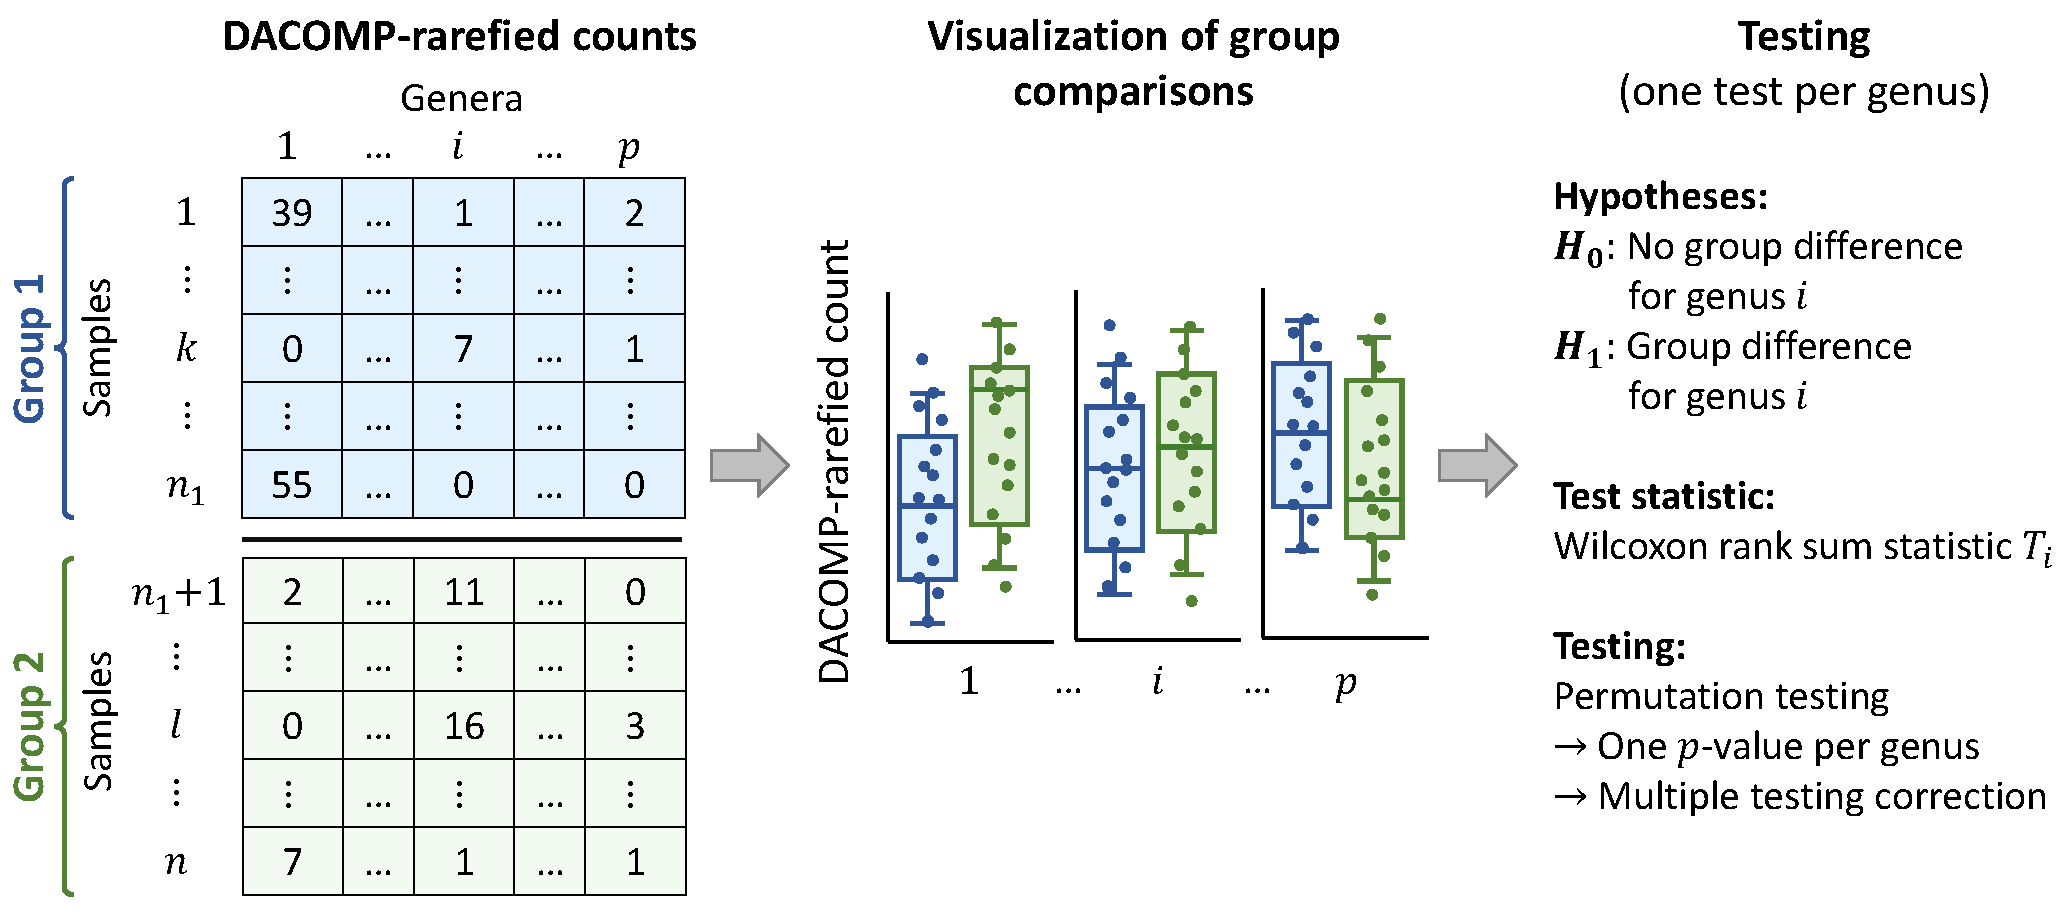
\includegraphics[width=\textwidth]{../ch04_feature_level/overview_figures/overview_diff_abundance.pdf}
	\caption{\textbf{Overview of differential abundance analysis with DACOMP.} DACOMP-rarefied counts are compared between groups separately for each tested genus. Group-wise distributions can be inspected descriptively, whereas formal inference is based on a taxon-specific Wilcoxon rank-sum statistic and a permutation test. This yields one $p$-value per genus, which is subsequently adjusted for multiple testing.}
	\label{fig:4feature:overview_diff_abundance}
\end{figure}

%====================================
\subsection{Overview of existing methods}
\label{sec:4feature:diffabund_overview}
%====================================

A large number of methods have been proposed for differential abundance analysis, reflecting the fact that no single modeling strategy resolves all statistical difficulties of microbiome data. A first group of methods adapts count-based models originally developed for RNA-seq data. Widely used examples include edgeR \citep{robinson2010edger}, DESeq2 \citep{love2014moderated}, and metagenomeSeq \citep{paulson2013differential}. These methods model taxon-specific counts and account for overdispersion, often through negative binomial or zero-inflated models combined with sample-specific normalization factors. Their main advantage is that they provide a well-established framework for high-dimensional count data, including variance estimation and multiple testing correction. However, their interpretation in microbiome applications depends strongly on the adequacy of the normalization strategy and on assumptions about the majority of features being unchanged across groups. Since microbiome data are compositional, such assumptions are not merely technical but affect the biological meaning of the resulting differential abundance calls.

A second group of methods is based more explicitly on compositional data analysis. These approaches start from the observation that only relative information is available and that taxon abundances should therefore be interpreted through ratios or log-ratios. ALDEx2 \citep{fernandes2014unifying}, for example, uses Monte Carlo instances drawn from a Dirichlet model and performs testing on centered log-ratio transformed values. ANCOM \citep{mandal2015analysis} evaluates log-ratios between taxa and identifies features whose ratios to many other features differ between groups. These methods reduce the risk of detecting spurious effects caused by the constant-sum constraint, but they also make explicit that differential abundance in relative data is inherently comparative: a taxon is not assessed in isolation, but relative to other taxa or to a chosen reference structure.

More recent methods further refine this idea by estimating bias terms, selecting reference features, or formulating differential abundance in terms of compositional contrasts. ANCOM-BC \citep{lin2020analysis} introduces a bias-correction framework to account for sampling fractions, while LinDA \citep{zhou2022linda} uses linear models on centered log-ratio transformed data and aims to correct the compositional bias under sparsity. DACOMP \citep{brill2022testing} follows a reference-based strategy and performs differential abundance testing after selecting a set of taxa assumed to be non-differential. These methods differ in how they define the target of inference, how they handle the compositional constraint, and whether inference is based on asymptotic approximations, model-based assumptions, or resampling procedures.

Comparative studies have shown that differential abundance methods can yield substantially different results on the same data set, and that their performance depends on characteristics such as sparsity, sample size, effect size distribution, library size variability, and the proportion of truly differential taxa \citep{weiss2017normalization,nearing2022microbiome}. This variability is not surprising because different methods encode different assumptions about the data-generating process and about what it means for a taxon to be differentially abundant. Consequently, the choice of method should be guided by the scientific question, the data structure, and the intended interpretation of the results rather than by software availability alone.

In this thesis, the focus is on differential abundance analysis as a feature-wise comparative task under compositional constraints. For the application in Chapter~7, DACOMP is used because it explicitly addresses compositionality through a reference-based construction and relies on permutation-based inference. This makes it particularly suitable for connecting feature-level microbiome testing with the \texttt{permApprox} framework developed in Chapter~6. After introducing DACOMP in the next subsection, we describe how small DACOMP p-values can be refined using \texttt{permApprox} to reduce the finite-resolution limitations of empirical permutation testing.

%====================================
\subsection{DACOMP}
\label{sec:4feature:dacomp}
%====================================

DACOMP is a differential abundance method designed for compositional count data with potentially many zero counts \citep{brill2022testing}. In contrast to log-ratio based approaches such as the CLR transformation, DACOMP does not first transform the full composition into log-ratio coordinates. Instead, it accounts for compositionality through a reference-based testing strategy. The method is implemented in the \texttt{dacomp} R package and is based on the idea that differential abundance of an individual taxon cannot be inferred from its raw counts alone. As discussed in Chapter~\ref{ch:microbiome}, the total sequencing depth in microbiome data is arbitrary and the observed counts of all taxa are constrained to sum to this depth. Thus, an apparent change in the count or relative abundance of one taxon may be caused by a change in that taxon, by changes in other taxa, or by the compositional constraint itself. DACOMP addresses this problem by testing each candidate taxon relative to a set of reference taxa that are assumed to be non-differential with respect to the phenotype or group variable. These reference taxa serve as an internal comparison background, so that the candidate taxon is evaluated relative to taxa that are assumed to be stable rather than relative to the full sample total.

The reference set $\mathcal{B}$ is constructed from the data by identifying taxa whose log-ratios relative to all other taxa vary only weakly across samples. Let $X = (X_{ki}) \in \mathbb{N}_0^{n \times p}$ denote the count matrix, where $X_{ki}$ is the count of taxon $i$ in sample $k$. For each taxon~$i$, DACOMP considers pairwise log-ratios of the form
\begin{equation}
	\log_{10}\!\left(\frac{X_{ki}+1}{X_{k\ell}+1}\right), \qquad \ell \neq i,
	\label{eq:4feature:dacomp_log_ratios}
\end{equation}
where the pseudo-count avoids undefined ratios in the presence of zeros. The variability of these log-ratios across samples is summarized by a score $S_i$. Taxa with $S_i \leq S_{\mathrm{crit}}$ are selected as reference taxa, where $S_{\mathrm{crit}}$ is chosen such that the total number of reference reads per sample remains in a practical range. In this way, DACOMP aims to construct a reference set that is sufficiently stable across samples while still large enough to support the subsequent rarefaction-based testing procedure.

\newpage
For a candidate taxon $i \notin \mathcal{B}$, DACOMP compares the abundance of taxon $i$ with the total abundance of the reference taxa. Let
\begin{equation}
	R_k = \sum_{\ell \in \mathcal{B}} X_{k\ell}
	\label{eq:4feature:dacomp_reference_abundance}
\end{equation}
denote the total reference abundance in sample $k$. DACOMP then defines the common rarefaction depth
\begin{equation}
	\lambda = \min_{1 \leq k \leq n} R_k.
	\label{eq:4feature:dacomp_rarefaction_depth}
\end{equation}
For each sample $k$, a rarefied count $Z_{ki}$ is generated by sampling $\lambda$ reads without replacement from the pool consisting of taxon $i$ and the reference taxa. Equivalently, writing the hypergeometric distribution in terms of population size, number of candidate-taxon reads, and number of draws,
\begin{equation}
	Z_{ki} \sim \operatorname{Hypergeometric}\!\left(X_{ki}+R_k, X_{ki}, \lambda\right).
	\label{eq:4feature:dacomp_rarefied_counts}
\end{equation}
The rarefaction step places samples on a comparable scale with respect to the reference taxa and avoids relying on a parametric model for the original count distribution.

The feature-wise test statistic is then computed from the rarefied counts. In the two-group setting, let $Y_k \in \{0,1\}$ denote the group label of sample $k$. DACOMP uses the Wilcoxon rank-sum statistic
\begin{equation}
	T_i = \sum_{k:Y_k = 1} \operatorname{rank}(Z_{ki})
	\label{eq:4feature:dacomp_test_statistic}
\end{equation}
to compare the rarefied counts between groups. The corresponding null hypothesis can be formulated as
\begin{equation}
	H_{0i}: \text{taxon } i \text{ is not differentially abundant relative to the reference set } \mathcal{B}.
	\label{eq:4feature:dacomp_null}
\end{equation}
Because the test is based on ranks of rarefied counts, DACOMP avoids specifying a full parametric model for the taxon counts. This is advantageous in microbiome data, where sparsity, overdispersion, and excess zeros make simple distributional assumptions difficult to justify.

Inference is performed by permutation of the group labels. For each taxon $i$, the observed statistic $T_i$ is compared with a permutation distribution $\{T_i^{*(b)}\}_{b=1}^B$ obtained by repeatedly shuffling the labels $Y_k$ and recalculating the statistic. This yields empirical permutation p-values for all candidate taxa. The use of permutation testing makes DACOMP flexible and well suited to the feature-wise comparative setting considered in this thesis. At the same time, the resulting p-values are limited by the finite number of permutations: with $B$ permutations, empirical p-values lie on a discrete grid, which can be restrictive after multiple testing correction. This limitation is addressed in Chapter~\ref{ch:permapprox}, where the \texttt{permApprox} framework is introduced for refining small permutation p-values. Since \texttt{dacomp} exports both the observed statistic $T_i$ and the permuted statistics $\{T_i^{*(b)}\}_{b=1}^B$, its output can be used directly as input for \texttt{permApprox}. In the application chapter, DACOMP is therefore used for differential abundance testing, and small permutation p-values are refined with \texttt{permApprox} as a post-processing step.

%%%%%%%%%%%%%%%%%%%%%%%%%%%%%%%%%%%%%
\section{Differential distribution analysis}
\label{sec:4feature:diffdist}
%%%%%%%%%%%%%%%%%%%%%%%%%%%%%%%%%%%%%

\begin{figure}[H]
	\centering
	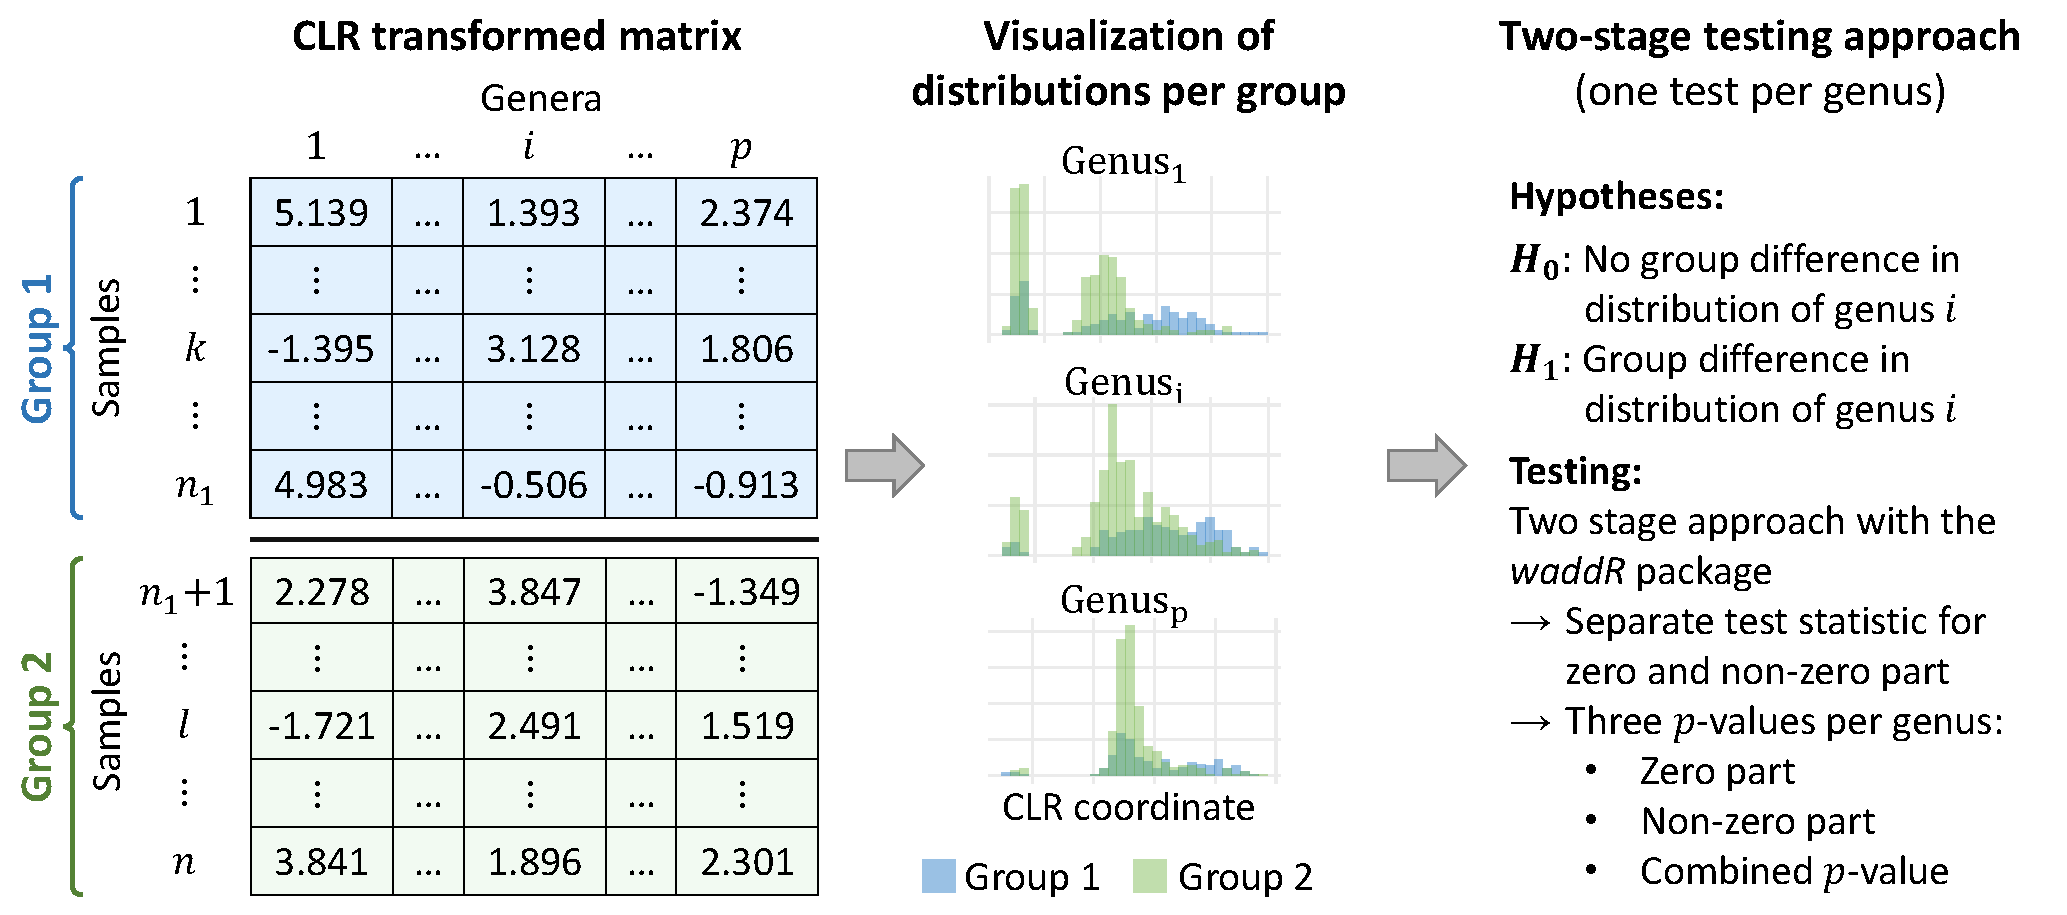
\includegraphics[width=\textwidth]{../ch04_feature_level/overview_figures/overview_diff_distribution.pdf}
	\caption{\textbf{Overview of differential distribution analysis with \texttt{waddR}.} For each genus, the group-specific distributions of CLR-transformed values are compared. The \texttt{waddR} framework separates differences in the frequency of observed zeros from differences in the distribution of CLR values among samples with positive original counts. The resulting zero-part and non-zero-part $p$-values can be combined into an overall $p$-value for each tested genus.}
	\label{fig:4feature:overview_diff_distribution}
\end{figure}

Differential abundance analysis aims to identify taxa whose abundance levels differ between groups. In many applications, however, group differences may go beyond a shift in mean or median abundance. A taxon may have similar average abundance in two groups but differ in variability, zero frequency, skewness, multimodality, or other aspects of distributional shape. Such differences can be biologically relevant, for example when a taxon is consistently present in one group but occurs only in a subset of individuals in another group. Differential distribution analysis therefore asks the more general question of whether the full feature-specific distribution differs between groups.
Figure~\ref{fig:4feature:overview_diff_distribution} illustrates this feature-wise perspective for the two-stage \texttt{waddR} framework, which separately considers differences in zero frequencies and in the distributions of non-zero CLR values.

For taxon $i$, let $F_i^{(1)}$ and $F_i^{(2)}$ denote the distributions of the preprocessed abundance values in the two groups with sample sizes $n_1$ and $n_2$. Differential distribution analysis considers the null hypothesis
\begin{equation}
\label{eq:4feature:diffdist_null}
H_{0i}: F_i^{(1)} = F_i^{(2)}.
\end{equation}
This null hypothesis is broader than a null hypothesis on a single location parameter. It is violated not only by differences in mean abundance, but also by differences in variance, zero structure, tail behavior, or modality. The price of this broader alternative is that distributional tests may be less specific: a significant result indicates that the distributions differ, but does not automatically identify which aspect of the distribution is responsible.

Compared with differential abundance analysis, differential distribution analysis is less standardized in microbiome research. The following subsection therefore briefly reviews classical distributional two-sample tests and more recent approaches developed for high-throughput single-cell data. The subsequent subsection then focuses on \texttt{waddR}, which is used in the application chapter and is particularly relevant for this thesis because of its connection to permutation testing and GPD-based p-value approximation.

%====================================
\subsection{Overview of existing methods}
\label{sec:4feature:diffdist_overview}
%====================================

Classical nonparametric two-sample tests already provide tools for testing equality of one-dimensional distributions. A prominent example is the two-sample Kolmogorov--Smirnov test \citep{kolmogorov1933sulla,smirnov1948table}. Let $\hat F_i^{(1)}$ and $\hat F_i^{(2)}$ denote the empirical distribution functions of taxon $i$ in the two groups. The Kolmogorov--Smirnov statistic is defined as
\begin{equation}
\label{eq:ks_statistic}
D_i = \sup_x \left| \hat F_i^{(1)}(x) - \hat F_i^{(2)}(x) \right|.
\end{equation}
It measures the largest vertical distance between the two empirical cumulative distribution functions. The test is sensitive to localized discrepancies between distributions and is distribution-free under continuity assumptions. However, microbiome data often contain many ties and zeros, so the usual continuous-distribution theory is not directly applicable. In such settings, permutation-based p-values are more appropriate, but they again inherit the finite-resolution problem discussed in Chapter~\ref{ch:permapprox}.

Other classical tests compare empirical distribution functions through integrated rather than supremum-type distances. Cramér--von Mises-type statistics integrate squared differences between distribution functions \citep{cramer1928composition,vonmises1928wahrscheinlichkeit}, while Anderson--Darling-type tests use a weighting that gives more emphasis to tail differences \citep{anderson1952asymptotic}. These tests are also designed to detect general distributional differences, but their interpretation remains global: they test whether the distributions differ without directly separating location, scale, and shape effects.

More recent differential distribution methods have been developed mainly in the context of single-cell data analysis, where full expression distributions across cells are of scientific interest. The method \texttt{scDD}, for example, uses a Bayesian mixture modeling framework to classify genes according to different types of distributional changes, including changes in modality and in the proportions of cells assigned to expression components \citep{korthauer2016statistical}. The method \texttt{distinct} provides a general framework for differential distribution analysis that is particularly suited to single-cell and cytometry data, where differences may occur in complex distributional features rather than only in mean expression \citep{tiberi2023distinct}. These methods illustrate that distributional testing is useful when heterogeneity itself is part of the biological signal.

Among the more specialized approaches, \texttt{waddR} provides a Wasserstein-based framework for testing differential distributions \citep{schefzik2021fast}. In contrast to the Kolmogorov--Smirnov statistic, which is based on the maximum distance between empirical distribution functions, the 2-Wasserstein distance compares distributions through their quantile functions. For two one-dimensional distributions $F_i^{(1)}$ and $F_i^{(2)}$, the squared 2-Wasserstein distance can be written as
\begin{equation}
\label{eq:wasserstein_distance}
W_2^2\left(F_i^{(1)},F_i^{(2)}\right) = \int_0^1 \left( \left(F_i^{(1)}\right)^{-1}(u) - \left(F_i^{(2)}\right)^{-1}(u) \right)^2 \, \mathrm{d}u.
\end{equation}
This distance has an intuitive interpretation as the amount of transport required to transform one distribution into the other. Moreover, in one dimension, the squared 2-Wasserstein distance admits a decomposition into location, size, and shape components. The decomposition separates contributions related to location, variability, and residual shape differences after centering and scaling. This decomposition is useful because it provides more insight into the nature of a detected distributional difference than a single global p-value alone.

Although methods such as \texttt{scDD}, \texttt{distinct}, and \texttt{waddR} were primarily motivated by single-cell applications, the statistical question they address is not restricted to single-cell data. They can also be considered for microbiome feature-level analysis when the aim is to test whether the distribution of a taxon differs between groups beyond a simple abundance shift. In this thesis, we focus on \texttt{waddR} for two reasons. First, it provides a direct feature-wise test for equality of one-dimensional distributions and decomposes the squared 2-Wasserstein distance into interpretable components. Second, the workflow already includes a generalized Pareto distribution (GPD) approximation for small permutation p-values. This makes \texttt{waddR} particularly suitable for comparison with the constrained GPD-based p-value refinement developed in Chapter~\ref{ch:permapprox}.

%====================================
\subsection{Two-stage differential distribution testing with \texttt{waddR}}
\label{sec:4feature:diffdist_waddr}
%====================================

The \texttt{waddR} approach provides a Wasserstein-based framework for testing differential distributions in high-throughput data \citep{schefzik2021fast}. For each feature, the method compares the distributions observed in two groups using the squared 2-Wasserstein distance. As introduced above, this distance compares one-dimensional distributions through their quantile functions and therefore captures differences in the full distribution rather than only differences in a location parameter. This makes \texttt{waddR} particularly suitable for settings in which group differences may involve changes in variability, zero frequency, or distributional shape.

A specific feature of \texttt{waddR} is its two-stage testing strategy for data with excess zeros. In the original single-cell setting, the first stage tests for differential proportions of zero observations between the two groups. This idea follows \texttt{scDD}: for each gene, a logistic regression model\footnote{The \texttt{waddR} paper refers to this step as Bayesian logistic regression. Since the cited \texttt{scDD} description formulates the zero test as logistic regression adjusted for cellular detection rate, we describe the step here in terms of the underlying regression model.} is fitted to the binary zero indicator and adjusted for the cellular detection rate, which accounts for differences in the number of detected genes per cell \citep{finak2015mast,korthauer2016statistical}. 

Let
\begin{equation}
\label{eq:waddr_zero_prob}
\pi_i^{(g)} = \Pr\left(X_i^{(g)} = 0\right), \qquad g \in \{1,2\},
\end{equation}
denote the group-specific zero probabilities for feature $i$. The corresponding null hypothesis is
\begin{equation}
\label{eq:waddr_zero_null}
H_{0i,0}: \pi_i^{(1)} = \pi_i^{(2)}.
\end{equation}
The zero stage yields a p-value $p_{i,0}$. We denote the corresponding Wald statistic for the group effect in the logistic regression model by $Z_{i,0}$.

The second stage restricts the analysis to the non-zero observations and tests whether their distributions differ between groups. Let $F_{i,+}^{(1)}$ and $F_{i,+}^{(2)}$ denote the group-specific distributions of the positive values of feature $i$. The corresponding null hypothesis is
\begin{equation}
\label{eq:waddr_nonzero_null}
H_{0i,+}: F_{i,+}^{(1)} = F_{i,+}^{(2)}.
\end{equation}
The test statistic for the non-zero stage is the squared 2-Wasserstein distance
\begin{equation}
\label{eq:4feature:waddr_nonzero_statistic}
T_{i,+} = W_2^2\left(F_{i,+}^{(1)},F_{i,+}^{(2)}\right).
\end{equation}
Large values of $T_{i,+}$ indicate stronger evidence against equality of the non-zero distributions. This stage yields a p-value $p_{i,+}$ for differential distributions among the non-zero observations.

The two p-values from the zero and non-zero parts can be combined into an overall p-value using Fisher's method \citep{fisher1925statistical}. For feature $i$, the Fisher statistic is
\begin{equation}
\label{eq:waddr_fisher}
C_i = -2\left(\log p_{i,0} + \log p_{i,+}\right).
\end{equation}
Under the classical Fisher combination framework, and assuming independence of the two component p-values under the joint null hypothesis, $C_i$ is compared with a chi-squared distribution with four degrees of freedom, leading to a combined p-value
\begin{equation}
\label{eq:4feature:waddr_combined_pvalue}
p_{i,\mathrm{comb}} = \Pr\left(\chi^2_4 \geq C_i\right).
\end{equation}
The resulting p-value summarizes evidence from both components, while the separate p-values retain information about whether the signal is driven by zero frequency, non-zero distributional differences, or both.

%====================================
\subsection{Adaptation of \texttt{waddR} to microbiome data}
\label{sec:4feature:diffdist_waddr_microbiome}
%====================================

In principle, \texttt{waddR}'s two-stage idea is also relevant for microbiome data, where zeros are frequent and may carry biological or technical information. However, the original \texttt{waddR} implementation assumes non-negative expression values. In its two-stage wrapper, non-zero observations are identified by retaining values larger than zero. This is appropriate for count-like single-cell expression data, but it is not appropriate after CLR transformation, where negative values simply indicate below-geometric-mean relative abundance rather than absence.

For microbiome data, we therefore use an adapted two-stage strategy. The count matrix is first transformed to relative abundances, zeros are handled by multiplicative replacement, and the resulting strictly positive compositions are transformed using the CLR transformation, following the preprocessing choices in Section~\ref{sec:2micro:preprocessing_choices_thesis}. The zero stage is nevertheless defined on the original count scale: a sample is treated as zero for taxon $i$ if the original count of that taxon is zero. The zero-stage p-value $p_{i,0}$ therefore tests for differences in original zero frequencies between groups.

For the non-zero Wasserstein stage, zeros are again defined on the original count scale, but the tested values are taken from the CLR-transformed matrix. Thus, for each taxon, we retain samples with positive original counts and compare the corresponding CLR values between groups. Let $Z_i$ denote the CLR-transformed coordinate of taxon $i$, and let $F_{i,+}^{(g)}$ denote the distribution of $Z_i^{(g)}$ among samples with $X_i^{(g)} > 0$. The non-zero null hypothesis remains
\begin{equation}
H_{0i,+}: F_{i,+}^{(1)} = F_{i,+}^{(2)},
\end{equation}
but it is now interpreted as equality of the CLR-transformed distributions among originally observed values. Negative CLR values are retained whenever the original count is non-zero. This preserves the two-stage interpretation while avoiding the erroneous removal of negative CLR coordinates.

For the non-zero part, we use the semi-parametric Wasserstein permutation test implemented in \texttt{waddR}. For each feature $i$, the observed statistic $T_i$ is compared with a permutation distribution $\{T_i^{*(b)}\}_{b=1}^B$ obtained by shuffling the group labels and recalculating the Wasserstein statistic in \eqref{eq:4feature:waddr_nonzero_statistic}. Since permutation testing can become computationally demanding when many features are tested, \texttt{waddR} provides a semi-parametric p-value approximation based on the generalized Pareto distribution for small permutation p-values. This is directly connected to the finite-resolution problem discussed in Chapter~\ref{ch:permapprox}: with a limited number of permutations, empirical p-values are restricted to a coarse grid and may be insufficiently resolved in the tail.

In the application in Chapter~\ref{ch:application}, the GPD approximation used by \texttt{waddR} produced many zero p-values for the non-zero distributional test. Such zero p-values are problematic for the reasons discussed in Chapter~\ref{ch:permapprox}: they are not valid permutation p-values, remain zero after multiple testing correction, and prevent a meaningful ranking of very strong signals. The aim of the \texttt{permApprox} refinement in this setting is therefore not primarily to compare GPD-based p-values with empirical permutation p-values. Rather, the central question is whether the constrained GPD approach implemented in \texttt{permApprox} can eliminate zero p-values while preserving the Wasserstein-based test statistic used by \texttt{waddR}.

A practical complication is that the original \texttt{waddR} output does not provide the complete matrix of permuted test statistics required by \texttt{permApprox}. The \texttt{permApprox} workflow requires, for each tested feature, the observed statistic $T_i$ together with the permutation statistics $\{T_i^{*(b)}\}_{b=1}^B$. We therefore use a modified R implementation of the \texttt{waddR} approach that exports these quantities for the non-zero distributional test. The exported observed and permuted Wasserstein statistics are then passed to \texttt{permApprox}, where p-values are recomputed using the constrained GPD-based refinement described in Chapter~\ref{ch:permapprox}.

Only the non-zero Wasserstein part is refined with \texttt{permApprox}. The zero-proportion p-value is kept separate and can be combined with the refined non-zero p-value using Fisher's method. This preserves the interpretability of the two-stage procedure while adapting it to compositional microbiome data: original counts determine zero status, CLR-transformed values define the non-zero distributions, and \texttt{permApprox} refines the permutation-based tail inference for the Wasserstein statistic.

% !TeX root = ../thesis.tex

%%%%%%%%%%%%%%%%%%%%%%%%%%%%%%%%%%%%%%%%%%
\thesischapter[ch:netcomi][0.75\textwidth]
  {``What is important, rather, is that all bridges are weak ties.''}
  {--- Mark S. Granovetter, 1973}
  {Association networks with NetCoMi}
\nocite{granovetter1973strength}
\chapterabstract{This chapter presents microbial association networks as relational representations of microbiome data and introduces \texttt{NetCoMi} as the first main methodological contribution of the thesis. It reviews key steps in network construction, including association estimation for compositional data, sparsification, and the quantification of node-level and global network properties. Building on these components, the chapter describes \texttt{NetCoMi} as an integrated workflow for constructing, analyzing, visualizing, and comparing microbial networks. Particular emphasis is placed on comparative network inference, where permutation-based procedures are used to assess differences in network properties between groups.}
\chaptercontents
%``Wherever we see life, we see networks.''
%--- Fritjof Capra
%%%%%%%%%%%%%%%%%%%%%%%%%%%%%%%%%%%%%%%%%%

\section*{Formal chapter information}

\subsection*{Author contributions}

The work presented in this chapter emerged from Stefanie Peschel's Master's thesis, which addressed the construction and comparison of microbial association networks and was carried out in collaboration with researchers at Helmholtz Zentrum München under the supervision of Prof.\ Dr.\ Anne-Laure Boulesteix. As part of this earlier work, Stefanie Peschel developed an initial version of the \texttt{NetCoMi} R package. This prototype implemented a focused workflow for constructing microbial association networks using a selected association estimation approach, analyzing the resulting networks, and comparing network properties between two groups. Comparative network analysis was therefore already a central component of the original project.

The work was subsequently expanded into one of the main methodological contributions of this dissertation under the supervision of Prof.\ Dr.\ Anne-Laure Boulesteix and Prof.\ Dr.\ Erika von Mutius at Helmholtz Zentrum München. Prof.\ Dr.\ Christian L.\ Müller provided substantial scientific guidance from an early stage on and was closely involved in the development of the project. Stefanie Peschel further developed the underlying workflow, extended the methodological scope of the package, implemented the software, prepared its documentation and tutorials, and conducted the real-data analyses presented in the accompanying publication. The resulting framework was published as \citet{peschel2021netcomi}, with Stefanie Peschel as first author. Since its publication, the \texttt{NetCoMi} package has been substantially further developed, with additional functionality implemented over time. The project was completed under the direct supervision of Prof.\ Dr.\ Christian L.\ Müller.

\subsection*{Code and software availability}

The code and graphical material used to generate the figures and examples presented in this chapter are included in the thesis repository archived on Zenodo \citep{Peschel2026thesisRepo}. The material belonging to this chapter is provided in the folder \href{https://github.com/stefpeschel/phd_thesis/tree/main/ch05_NetCoMi}{\texttt{ch05\_NetCoMi}}.

The \texttt{NetCoMi} R package implementing the workflow described in this chapter is openly available at: \url{https://github.com/stefpeschel/NetCoMi}

A structured package website, including installation instructions, reference documentation, and tutorials, is available at: \url{https://NetCoMi.de}

\subsection*{Note on publication}

The central methodological framework presented in this chapter was originally published in the following article, where Stefanie Peschel is first author:

\begin{itemize}
\item Stefanie Peschel, Christian L.\ Müller, Erika von Mutius, Anne-Laure Boulesteix, and Martin Depner. (2021). \texttt{NetCoMi}: Network construction and comparison for microbiome data in R. \textit{Briefings in Bioinformatics}, 22(4), bbaa290. \url{https://doi.org/10.1093/bib/bbaa290}
\end{itemize}

The article is published under the Creative Commons Attribution License, which permits unrestricted use, distribution, and reproduction provided that the original work is appropriately cited.

\subsection*{Related contributions and dissemination}

The \texttt{NetCoMi} framework has also contributed to further methodological and educational work. Stefanie Peschel is a co-author of \citet{ullmann2023overoptimism}, which used \texttt{NetCoMi} to investigate over-optimism in unsupervised microbiome analysis. The study illustrates that exploring multiple plausible preprocessing and network-learning strategies, and subsequently focusing on the most favorable results, can lead to overly optimistic conclusions. This issue is revisited in the general discussion of this thesis.

Stefanie Peschel also contributed to the network-related content of \textit{Applied Microbiome Statistics: Correlation, Association, Interaction and Composition} by \citet{xia2024applied}. In particular, she provided methodological advice, code examples, and feedback on the chapters addressing microbial network construction and comparison. She is acknowledged in the book but is not a co-author.

In addition, Stefanie Peschel co-authored the online book and accompanying preprint \citet{borman2025orchestrating}. Within the \textit{Orchestrating Microbiome Analysis} workflow, she contributed chapters on network learning, network analysis, and network comparison, which demonstrate the use of \texttt{NetCoMi} within a broader Bioconductor-based microbiome analysis framework.

\subsection*{Note on additional results}

The present chapter substantially extends the published \texttt{NetCoMi} article. In addition to describing the integrated workflow introduced in the original publication, it documents methodological developments and additional functionality that have been implemented in \texttt{NetCoMi} since its publication. More generally, the chapter discusses the challenges of designing and implementing a flexible network-analysis workflow that combines methods with different assumptions, preprocessing requirements, and data characteristics within a coherent and reproducible R package.

The chapter further elaborates on comparative network inference, including permutation-based testing of network properties. These procedures provide the original methodological motivation for Chapter~\ref{ch:permapprox}, where the limited resolution of permutation p-values under realistic computational budgets is addressed in greater detail.

\newpage
%%%%%%%%%%%%%%%%%%%%%%%%%%%%%%%%%%%%%
\section{Introduction}
\label{sec:5net:intro}
%%%%%%%%%%%%%%%%%%%%%%%%%%%%%%%%%%%%%

Association networks extend microbiome data analysis beyond marginal and aggregated characteristics by modeling relationships between microbial taxa. In contrast to community-level summaries (Chapter~\ref{ch:community}) and feature-level measures (Chapter~\ref{ch:feature}), which focus on global properties or individual taxa, network-based analysis considers dependencies between taxa and therefore combines aspects of both perspectives. This allows the investigation of how microbial features are associated within a community and how these association patterns differ across conditions.

This increased scope comes at the cost of additional methodological complexity. Microbial network analysis is not a single procedure, but a multi-step workflow that involves several modeling and analysis decisions. These include the estimation of associations between taxa, the construction of a network representation, the analysis of network properties, and, in comparative settings, the formal comparison of networks across groups.

An overview of this workflow is provided in Figure~\ref{fig:5net:workflow}, and the structure of this chapter follows its main components. Preprocessing is not discussed further here, as it has already been introduced in Chapter~\ref{ch:microbiome} and is equally relevant across all analysis targets. Sections~\ref{sec:5net:net_construction} to \ref{sec:5net:net_comparison} review the methodological foundations of network construction, network analysis, and network comparison. These sections highlight key challenges specific to microbiome data, including compositionality, sparsity, and the lack of analytically tractable null distributions for many network-based statistics.

\begin{figure}[!ht]
\centering

\includegraphics[width=\textwidth]{figures/NetCoMi/workflow.pdf}
\caption{
\textbf{Typical network analysis workflow for microbiome data.}
Section numbers indicate where the corresponding components are discussed.
Starting from a count matrix, the data are first preprocessed, including filtering, zero handling, and normalization (Sections~\ref{sec:2micro:filtering} to \ref{sec:2micro:normalization}). Based on the preprocessed data, pairwise associations between taxa are estimated, followed by sparsification and transformation steps to obtain an adjacency structure representing the network (Section~\ref{sec:5net:net_construction}). The resulting network can then be analyzed using node-level and global summary measures and visualized for interpretation (Section~\ref{sec:5net:net_analysis}). In comparative settings, the workflow is extended to include statistical procedures for network comparison, leading to the identification of differential network structures (Section~\ref{sec:5net:net_comparison}).
}
\label{fig:5net:workflow}
\end{figure}

Building on this foundation, the subsequent sections introduce the \texttt{NetCoMi} framework, which constitutes the first methodological contribution of this thesis. It integrates previously disjoint steps of microbial network analysis into a unified and modular workflow, enabling coherent and reproducible construction, analysis, and comparison of association networks. We discuss the motivation for this framework, address practical challenges arising from the combination of different methodological components, and present solutions for flexible and user-friendly network analysis.

A central aspect of comparative network analysis is the use of permutation-based testing procedures, as the distribution of many network-derived statistics is unknown. These methods form a direct link to Chapter~\ref{ch:permapprox}, where limitations of permutation testing under restricted computational budgets are addressed and improved $p$-value approximation methods are developed. Together, the approaches developed in this chapter and in Chapter~\ref{ch:permapprox} provide a coherent framework for statistically sound and computationally feasible network-based microbiome analysis.

%%%%%%%%%%%%%%%%%%%%%%%%%%%%%%%%%%%%%
\section{Network construction}
\label{sec:5net:net_construction}
%%%%%%%%%%%%%%%%%%%%%%%%%%%%%%%%%%%%%

Association network analysis aims to characterize relationships among microbial taxa within a cohort. In contrast to feature-level measures, which consider taxa marginally, network-based approaches explicitly model dependencies between taxa and represent them in the form of a graph or network. In the following, we use the terms \emph{graph} and \emph{network} interchangeably. While the term \emph{graph} originates from graph theory and refers to the underlying mathematical object, the term \emph{network} is more commonly used in applied contexts such as microbiome data analysis, where nodes and edges carry a domain-specific interpretation.

Formally, the objective is to estimate a graph $\mathcal{G} = (V, E)$, where the node set $V = \{1, \dots, p\}$ corresponds to microbial taxa and the edge set $E$ encodes statistical relationships between pairs of taxa. These relationships may represent marginal associations or conditional dependencies, depending on the chosen modeling framework. The resulting network is typically represented by an adjacency matrix $A = (a_{ij})$, where each entry $a_{ij}$ quantifies the presence and strength of a relationship between taxa $i$ and $j$.

Constructing such a network from microbiome data is a nontrivial task and involves several interconnected steps. In particular, one must (i) select an appropriate measure of association or dependency to quantify relationships between taxa, (ii) apply sparsification or regularization techniques to obtain a sparse and interpretable network, and (iii) transform the resulting associations into edge weights that define the adjacency structure. These steps jointly determine the topology and interpretability of the inferred network.

In the following subsections, we introduce the key components of this construction process. We begin with the estimation of pairwise associations between taxa, which forms the basis for all subsequent steps.

%====================================
\subsection{Sparse (inverse) covariance estimation}
\label{sec:5net:net_constr:sparse_cov_est}
%====================================

A natural starting point for quantifying relationships between microbial taxa is the use of classical association measures such as the Pearson or Spearman correlation coefficient. For two random variables $X$ and $Y$, the Pearson correlation is defined as
\begin{equation}
\rho(X,Y)=\frac{\mathrm{cov}(X,Y)}{\sigma_X \sigma_Y},
\end{equation}
where $\mathrm{cov}(X,Y)$ denotes the covariance between $X$ and $Y$, and $\sigma_X$, $\sigma_Y$ are the corresponding standard deviations \citep{schober2018correlation}. Estimating correlations from data therefore requires reliable estimation of the covariance structure.

In microbiome data analysis, covariance estimation is particularly challenging because the data characteristics described in Chapter~\ref{ch:microbiome} must be taken into account. Even after preprocessing to address differences in sequencing depth, excess zeros, and compositionality, one major difficulty remains: high dimensionality. In typical applications, the number of taxa $p$ is large relative to the number of samples $n$, often with $p \gg n$.

One might be tempted to use the sample covariance matrix as an estimator of $\rho(X,Y)$. For a data matrix $X \in \mathbb{R}^{n \times p}$ the sample covariance matrix is given by
\begin{equation}
S = \frac{1}{n-1} \sum_{i=1}^n (x_i - \bar{x})(x_i - \bar{x})^\top 
= \frac{1}{n-1} X^{*\top} X^*,
\end{equation}
where $X^*$ denotes the column-centered data matrix \citep{hastie2009elements}.
In the high-dimensional regime $p \gg n$, the sample covariance matrix $S$ has rank at most $n-1$ and is therefore singular. Consequently, it is not invertible, and covariance and correlation estimates derived from $S$ are unstable and may poorly reflect the underlying dependence structure.

To obtain meaningful estimates in such settings, additional structural assumptions are required. A common and crucial assumption is \emph{sparsity}, which postulates that only a relatively small number of pairwise associations are non-zero. This assumption is biologically plausible in many microbial ecosystems, where interactions tend to occur within limited subsets of taxa rather than across all pairs. From a statistical perspective, sparsity makes the high-dimensional estimation problem tractable by reducing the effective number of parameters and enabling regularization-based estimation techniques. Most methods for high-dimensional covariance and inverse covariance estimation discussed in this work therefore explicitly or implicitly rely on sparsity assumptions.

A classical remedy is covariance shrinkage. The approach of \citet{schafer2005shrinkage} replaces the sample covariance matrix $S$ by a convex combination
\begin{equation}
\hat{\Sigma} = (1-\lambda)S + \lambda T,
\end{equation}
where $T$ is a structured target matrix and $\lambda \in [0,1]$ is a shrinkage intensity chosen to minimize estimation error. In the formulation of Schäfer and Strimmer, the target is typically chosen as a low-dimensional matrix, for example the diagonal of $S$, and the shrinkage intensity is estimated analytically from the data. This yields a positive definite and well-conditioned covariance estimator in situations where the sample covariance matrix is singular or nearly singular. The resulting covariance estimate can then be standardized to obtain a correlation matrix,
\begin{equation}
\hat{\rho}_{ij}=\frac{\hat{\sigma}_{ij}}{\sqrt{\hat{\sigma}_{ii}\hat{\sigma}_{jj}}},
\end{equation}
where $\hat{\sigma}_{ij}$ denotes the $(i,j)$-th entry of $\hat{\Sigma}$.
The \texttt{corpcor} package \citep{schafer2021corpcor} provides an implementation of this approach via \texttt{cor.shrink()}, which is also used by \texttt{NetCoMi}.

Besides shrinkage-based approaches, further methods have been proposed to directly estimate sparse covariance matrices by imposing structural assumptions or regularization. 
For instance, \citet{bickel2008regularized} propose banding and tapering estimators of the sample covariance matrix, which set entries far from the diagonal to zero or shrink them towards zero, exploiting an ordering assumption under which variables that are far apart are approximately independent.  
In a different direction, \citet{bien2011sparse} propose a convex optimization approach that estimates a sparse covariance matrix by penalizing the Gaussian log-likelihood with a Lasso penalty on the entries of the covariance matrix, thereby encouraging sparsity directly in the covariance structure.

Beyond these generally applicable methods, a number of approaches have been specifically developed for microbiome data, taking into account compositionality and other data-specific characteristics. Prominent examples include SparCC \citep{friedman2012inferring} and CCLasso \citep{fang2015cclasso}, which will be discussed in more detail in the following subsection.

Beyond the statistical challenge of covariance estimation, a conceptual distinction is required between two different notions of association. Correlation-based approaches quantify marginal associations between taxa and thus capture co-variation patterns, but they do not distinguish whether an observed relationship is direct or induced indirectly through other taxa. If the aim is instead to identify direct pairwise relationships after accounting for the remaining community members, conditional dependence is the more appropriate target.

A common framework for modeling such conditional relationships is given by graphical models, in which the dependency structure between variables is encoded in the inverse covariance (precision) matrix $\Omega = \Sigma^{-1}$. In this setting, zeros in $\Omega$ correspond to conditional independencies between pairs of variables under suitable distributional assumptions \citep{kurtz2015sparse}. From an estimate $\hat{\Omega}$, partial correlations can be obtained as
\begin{equation}
\hat{\tilde{\rho}}_{ij}
=
-\frac{\hat{\omega}_{ij}}{\sqrt{\hat{\omega}_{ii}\hat{\omega}_{jj}}},
\end{equation}
where $\hat{\omega}_{ij}$ denotes the $(i,j)$-th entry of $\hat{\Omega}$.

Accordingly, one possible strategy is to estimate a sparse covariance matrix, invert it to obtain a precision matrix, and then derive partial correlations. Alternatively, one may estimate the sparse inverse covariance matrix directly using dedicated methods such as neighborhood selection \citep{meinshausen2006highdimensional}, the graphical lasso \citep{friedman2008sparse}, or CLIME \citep{cai2011constrained}. These approaches differ in their estimation principles but share the goal of recovering a sparse conditional dependence structure in high-dimensional settings. 

The relationship between covariance, precision, and (partial) correlation matrices is summarized in Figure~\ref{fig:5net:sparse_cov_estimation}.
Dedicated methods for microbiome data, such as SparCC for sparse correlation estimation and SPIEC-EASI for sparse inverse covariance estimation, are discussed in the next subsection.


\begin{figure}[H]
\centering
\includegraphics[width=\textwidth]{figures/NetCoMi/sparse_cov_estimation.pdf}
\caption{\textbf{From covariance estimation to correlation and partial correlation.} Overview of high-dimensional association estimation after preprocessing. The upper path illustrates sparse covariance estimation followed by standardization to a sparse correlation matrix. The lower path illustrates sparse inverse covariance estimation and the resulting partial correlation matrix. Examples of microbiome-specific methods are indicated for both branches (SparCC and SpiecEasi).}
\label{fig:5net:sparse_cov_estimation}
\end{figure}

%====================================
\subsection{Association estimation for microbiome data}
\label{sec:5net:net_constr:asso_microbiome}
%====================================

In the previous subsection, we outlined general strategies for estimating sparse correlation matrices and their partial counterparts after accounting for the typical characteristics of microbiome data described in Chapter~\ref{ch:microbiome}. However, over the last decade, a variety of methods have been specifically developed for microbiome data, which explicitly incorporate compositionality, sparsity, and zero inflation into the proposed approach. In many cases, these methods integrate parts of the preprocessing steps described in Chapter~\ref{ch:microbiome} directly into the model formulation.

In the following, we introduce representative approaches for estimating both marginal and conditional associations in microbiome data. In particular, we consider two widely used methods for correlation estimation, namely SparCC and CCLasso, and two approaches for estimating conditional dependencies based on sparse inverse covariance estimation, namely SPIEC-EASI and SPRING. In addition, we introduce proportionality as an alternative association measure tailored to compositional data, as well as a shrinkage-based extension proposed by \citet{badri2020shrinkage}.

%------------------------------------
\subsubsection{SparCC}
\label{sec:5net:net_constr:sparcc}
%------------------------------------

SparCC (Sparse Correlations for Compositional data) \citep{friedman2012inferring} is one of the most widely used methods for estimating correlations between microbial taxa from compositional data. It is based on the idea of approximating the Pearson correlation between the unobserved absolute abundances from log-ratio transformed data. Let $x_i$ and $x_j$ denote the (unobserved) absolute abundances of two taxa. SparCC exploits the relationship between correlations and the variance of log-ratios,
\begin{equation}
t_{ij} = \mathrm{Var}\left(\log\frac{x_i}{x_j}\right),
\end{equation}
which can be expressed in terms of the variances and covariances of the log-transformed abundances. Under the assumption that the number of taxa is large and that the correlation structure is sparse, this system of equations can be approximated and solved to obtain estimates of the underlying correlations.

An important practical aspect of SparCC is the treatment of zeros, since log-ratios are undefined for zero counts. \citet{friedman2012inferring} propose a Bayesian approach in which the observed counts are interpreted as draws from a multinomial distribution with Dirichlet prior. The resulting posterior distribution is then used to generate strictly positive pseudo-counts, enabling log-ratio computations.

The sparsity assumption is further incorporated through an iterative procedure in which pairs of taxa with large estimated correlations are successively excluded from the estimation process. This step aims to reduce the influence of strong associations that would otherwise violate the approximation underlying the method. To account for variability introduced by the resampling procedure, the entire algorithm is typically repeated multiple times, and the final correlation estimates are obtained by averaging over repetitions.

%------------------------------------
\subsubsection{CCLasso}
\label{sec:5net:net_constr:cclasso}
%------------------------------------

CCLasso (Correlation inference for Compositional data through Lasso) \citep{fang2015cclasso} is an alternative approach for inferring latent correlations between microbial taxa from compositional data. As in SparCC, log-ratio transformations are used to mitigate the effects of compositionality. In contrast to SparCC, however, CCLasso does not include an explicit strategy for handling zeros, so that zero replacement must be performed as a preprocessing step.

The method is based on the assumption that the underlying correlation structure is sparse, which allows the covariance and correlation matrices of the unobserved absolute abundances to be inferred from compositional data. CCLasso formulates this task as a convex optimization problem, in which a positive definite correlation matrix with entries in $[-1,1]$ is estimated by minimizing a loss function together with an $\ell_1$-penalty. The loss function measures how well the estimated correlation matrix reproduces the covariance structure observed in the log-ratio transformed data, thereby ensuring a good fit to the observed compositional data. This term is complemented by an $\ell_1$-penalty on the off-diagonal elements, which enforces sparsity by shrinking weak correlations towards zero.

%------------------------------------
\subsubsection{SPIEC-EASI}
\label{sec:5net:net_constr:spieceasi}
%------------------------------------

SPIEC-EASI (Sparse InversE Covariance Estimation for Ecological Association Inference) \citep{kurtz2015sparse} estimates a sparse network of conditional dependencies between microbial taxa. The method is specifically designed for compositional microbiome data and incorporates several steps of the general workflow depicted in Figure~\ref{fig:5net:workflow}. In particular, it combines log-ratio transformation, sparse graphical-model estimation, and stability-based model selection within a single framework.

To account for compositionality, the observed count data are transformed using the centered log-ratio (CLR) transformation, as defined in Equation~\eqref{eq:2micro:CLR} in Section~\ref{sec:2micro:norm:log-ratios}. SPIEC-EASI then estimates a sparse conditional-dependence graph from the transformed data. It provides two alternative estimation approaches. The first is neighbourhood selection proposed by \citet{meinshausen2006highdimensional}, commonly referred to as the ``MB'' method. The second is sparse inverse covariance selection, also known as the graphical lasso, introduced by \citet{friedman2008sparse}. While the graphical lasso estimates the precision matrix jointly through a global optimization problem, the MB method reconstructs the graph in a node-wise manner. Since the MB method is used for network construction in the application chapter, it is described in more detail below following the formulation shown in SPIEC-EASI \citep{kurtz2015sparse}.


Let $\mathbf{Z} = (\mathbf{z}_1,\ldots,\mathbf{z}_p)$ denote the CLR-transformed data matrix, where $\mathbf{z}_i \in \mathbb{R}^n$ contains the transformed values of taxon $i$ across the $n$ samples. For each taxon $i$, the MB approach regresses $\mathbf{z}_i$ on all remaining taxa using an $\ell_1$-penalized linear regression model,
\begin{equation}
\label{eq:5net:spieceasi_mb}
\hat{\boldsymbol{\beta}}^{(i)}(\lambda) =
\underset{\boldsymbol{\beta}\in\mathbb{R}^{p-1}}{\arg\min}
\left\{\frac{1}{n}\left\|\mathbf{z}_i - \mathbf{Z}_{-i}\boldsymbol{\beta} \right\|_2^2
+
\lambda \left\|\boldsymbol{\beta}\right\|_1\right\}.
\end{equation}
where $\mathbf{Z}_{-i}$ denotes the matrix of all CLR-transformed taxa except taxon $i$, $\lambda \geq 0$ is a regularization parameter, and $|\boldsymbol{\beta}|_1 = \sum_{j=1}^{p-1} |\beta_j|$ denotes the $\ell_1$ norm. This is a typical Lasso regression problem \citep{tibshirani1996regression}. The penalty shrinks regression coefficients towards zero and sets many of them exactly to zero. Consequently, for a fixed value of $\lambda$, the non-zero coefficients identify the estimated local neighborhood of taxon $i$.

Because this procedure is repeated for every taxon, it initially yields two potentially different coefficient estimates for each pair of taxa: one from the regression of taxon $i$ on taxon $j$ and one from the regression of taxon $j$ on taxon $i$. These node-wise estimates must therefore be symmetrized to obtain an undirected network. SPIEC-EASI offers several symmetrization rules. For example, an edge may be retained when it is selected in at least one of the two regressions or only when it is selected in both. When weighted associations are required, the two directed coefficient estimates can additionally be combined, for example by their average. The resulting non-zero entries define the estimated conditional-dependence network.

Both the MB and graphical-lasso approaches rely on the assumption that the underlying conditional-dependence structure is sparse. Their regularization parameter $\lambda$ controls the degree of sparsity: larger values yield fewer selected edges, whereas smaller values yield denser graphs. SPIEC-EASI selects $\lambda$ using the Stability Approach to Regularization Selection (StARS) \citep{liu2010stability}. StARS repeatedly draws subsamples of the data, estimates networks over a sequence of regularization values, and evaluates how strongly individual edge selections vary across subsamples. The selected regularization level is chosen to keep this estimated edge instability below a user-defined threshold. Thus, SPIEC-EASI performs association estimation and sparsification jointly, so that no additional edge-selection step is required after fitting the model. Alternative sparsification strategies for association measures that do not include an internal model-selection procedure are discussed later in this section.

%------------------------------------
\subsubsection{SPRING}
\label{sec:5net:net_constr:spring}
%------------------------------------

SPRING (Semi-Parametric Rank-based approach for INference in Graphical models) \citep{yoon2019microbial} follows a similar workflow as SPIEC-EASI but is applicable to both quantitative and relative abundance data. In contrast to Gaussian graphical models, SPRING relies on a semi-parametric framework that is more robust to deviations from normality and can explicitly account for zero inflation.

The method assumes that the data arise from a truncated Gaussian copula model \citep{yoon2020sparse}, which extends the Gaussian copula model of \citet{liu2009nonparanormal} to accommodate excess zeros. Under this model, associations between taxa are captured through a latent correlation matrix. This matrix is estimated using a rank-based approach based on Kendall's $\tau$, combined with element-wise optimization of an inverse copula transformation.

Based on the estimated latent correlation matrix, sparse conditional dependencies are inferred using the MB neighborhood selection approach \citep{meinshausen2006highdimensional}. As in SPIEC-EASI, sparsity is controlled via $\ell_1$-regularization, and model selection is performed using StARS \citep{liu2010stability}.

SPRING was originally developed for quantitative microbiome profiling (QMP) data, where absolute abundances are measured rather than relative abundances. Such data can be obtained, for example, by combining sequencing-based relative abundance measurements with total microbial load estimates from quantitative PCR (qPCR) or flow cytometry. In this setting, the compositional constraint is alleviated, although zero inflation remains a key challenge. 

However, SPRING can also be applied to compositional data. In this case, it employs a modified centered log-ratio transformation (mCLR) that avoids the need for zero replacement. The mCLR transformation computes the geometric mean based only on positive components, applies the clr transformation to these values, and subsequently shifts nonzero entries to ensure strict positivity, while zero values remain unchanged.

%------------------------------------
\subsubsection{Proportionality}
\label{sec:5net:net_constr:proportionality}
%------------------------------------

\citet{lovell2015proportionality} propose proportionality as an alternative measure of association that is consistent with the compositional nature of microbiome data. The key observation is that proportionality between two quantities is invariant under scaling by a common factor.

Consider two positive quantities $\omega_i$ and $\omega_j$. If they are proportional, i.e.,
$\omega_i \propto \omega_j$,
then for any positive constant $c > 0$ it holds that
\begin{equation}
\frac{\omega_i}{c} \propto \frac{\omega_j}{c}.
\end{equation}
Thus, proportionality is preserved under normalization by a common total. This implies that the total sum is irrelevant for assessing proportional relationships, as it cancels out in the ratio.

This principle can be transferred to microbiome data. Let $\omega_{ki}$ denote the unobserved true absolute abundance of taxon $i$ in sample $k$, and let $m_k = \sum_{l=1}^p \omega_{kl}$ denote the corresponding total abundance across all taxa. In practice, we observe counts $x_{ki}$ that represent only a fraction of the true abundances, for example due to sequencing depth limitations. These observed counts can be interpreted as being proportional to the relative abundances $\omega_{ki}/m_k$. Although the absolute scale of the data is unknown, the relative relationships between taxa are preserved. Consequently, proportionality between taxa can be assessed based on the observed data $x_{ki}$, despite the absence of absolute abundance information.

\citet{lovell2015proportionality} quantify proportionality based on the variance of log-ratios:
$\mathrm{Var}\!\left(\log\frac{x_i}{x_j}\right)$.
This quantity is zero if the two taxa are perfectly proportional across samples. However, this variance is not directly comparable across pairs of taxa. To address this, scaled measures of proportionality have been proposed, most notably the $\phi$ and $\rho_p$ statistics \citep{lovell2015proportionality, quinn2017propr}, which are typically computed on CLR-transformed data.

In particular, the $\rho_p$ measure provides a correlation-like quantity defined as
\begin{equation}
\label{eq:prop_rho}
\rho_p(\log x_i, \log x_j) = 1 - \frac{\mathrm{Var}(\log(x_i/x_j))}{\mathrm{Var}(\log x_i) + \mathrm{Var}(\log x_j)},
\end{equation}
which takes values in $[-1,1]$, with $\rho_p = 1$ corresponding to perfect proportionality. Due to its similarity to correlation coefficients, $\rho_p$ can be used as an edge weight in association networks and is implemented in the R package \texttt{propr} \citep{quinn2017propr}.

Despite its advantages for compositional data, proportionality remains a marginal measure of association and does not distinguish between direct and indirect relationships. As a consequence, networks constructed from proportionality measures share similar limitations as correlation-based networks.

%------------------------------------
\subsubsection{Shrinkage proportionality}
\label{sec:5net:net_constr:prop_shrink}
%------------------------------------

As discussed above, proportionality measures such as $\rho_p$ are based on variances and covariances of log-transformed data. In particular, Equation~\eqref{eq:prop_rho} can be equivalently expressed as
\begin{equation}
\rho_p(\log x_i, \log x_j) = \frac{2\,\mathrm{cov}(\log x_i, \log x_j)}{\mathrm{Var}(\log x_i) + \mathrm{Var}(\log x_j)},
\end{equation}
which highlights that proportionality is fundamentally determined by covariance components. Consequently, its estimation inherits the same challenges as classical covariance estimation in high-dimensional settings, in particular when the number of taxa exceeds the number of samples. In such scenarios, empirical covariance estimates are unstable and can lead to highly variable and inflated association measures.

To address this issue, \citet{badri2020shrinkage} propose combining proportionality with shrinkage estimation. Since proportionality can be expressed in terms of covariance components, shrinkage techniques can be applied directly to the underlying covariance matrix. In particular, they build on the shrinkage framework of \citet{schafer2005shrinkage} introduced in Section~\ref{sec:5net:net_constr:sparse_cov_est}, where the empirical covariance matrix is regularized towards a structured target to obtain more stable estimates in high-dimensional settings.

Empirical results by \citet{badri2020shrinkage} demonstrate that shrinkage substantially increases the stability and consistency of both correlation- and proportionality-based association estimates, particularly in the low-sample regime. In particular, shrinkage reduces the occurrence of extreme association values and yields estimates that are closer to their large-sample counterparts.

%====================================
\subsection{Accounting for latent confounding in association estimation}
\label{sec:5net:net_constr:latent_var}
%====================================

A fundamental challenge in microbial association analysis is the presence of unobserved or unmeasured factors that influence multiple taxa simultaneously. Such latent variables may represent environmental conditions, host-specific effects, or technical artifacts, and can induce spurious associations if not properly accounted for. In particular, correlations arising from shared dependence on hidden factors may be misinterpreted as direct microbial interactions, thereby distorting the inferred network structure.

To address this issue, \citet{kurtz2019disentangling} proposed a latent variable extension of sparse graphical models for microbial association estimation. Their approach explicitly accounts for hidden sources of variation by incorporating latent components into the precision matrix estimation. In this approach, the inverse covariance (precision) matrix $\Theta$ is decomposed into two components,
\begin{equation}
\Theta = S - L,
\end{equation}
where $S$ is a sparse matrix representing direct conditional dependencies between taxa, and $L$ is a low-rank matrix capturing the contribution of latent variables. The low-rank structure reflects the assumption that a small number of unobserved factors induces global correlations across taxa.

Estimation is typically based on a penalized likelihood approach that promotes both sparsity and low rank. Specifically, the parameters are obtained by minimizing a loss function with penalty
\begin{equation}
P(\Theta) = P(S,L) = \|S\|_1 + \beta \|L\|_*,
\end{equation}
where the $\ell_1$ norm $\|S\|_1$ encourages sparsity in $S$, the nuclear norm $\|L\|_*$ serves as a convex surrogate for the rank of $L$, and the parameter $\beta \geq 0$ controls the relative contribution of the latent component. This formulation allows for the simultaneous recovery of direct associations and latent effects.
In the context of microbiome data, this approach has been implemented in the \texttt{SpiecEasi} framework, where it is referred to as ``sparse and low rank'' (slr) approach.

%====================================
\subsection{Sparsification}
\label{sec:5net:net_constr:sparsification}
%====================================

Association measures typically yield dense matrices, in which nearly all pairs of taxa exhibit nonzero associations. However, such fully connected networks are difficult to interpret and often reflect noise rather than meaningful biological relationships. Sparsification is therefore a crucial step in network construction, aiming to retain only the most relevant associations and to obtain a stable and interpretable graph structure.

Sparsification has already been introduced in the previous section as part of model-based network inference methods. In particular, SPIEC-EASI and SPRING incorporate sparsification through the Stability Approach to Regularization Selection (StARS) \citep{liu2010stability}, which selects the sparsity parameter based on edge stability across subsamples.

In addition, sparsification can be performed as a separate step after association estimation. In the following, we discuss three broadly applicable approaches: thresholding, parametric inference, and resampling-based inference.

\subsubsection*{Thresholding}
The simplest and most widely applicable approach is to apply a threshold to the estimated association matrix. Associations are retained only if their absolute value exceeds a predefined threshold $\tau$, i.e.,
\begin{equation}
\tilde{\theta}_{ij} = 
\begin{cases}
\hat{\theta}_{ij}, & \text{if } |\hat{\theta}_{ij}| > \tau, \\
0, & \text{otherwise},
\end{cases}
\end{equation}
where $\hat{\theta}_{ij}$ denotes the estimated association between taxa $i$ and $j$, and $\tilde{\theta}_{ij}$ the sparsified value. This approach is computationally efficient and can be applied to any type of association measure, including correlations, proportionality, and conditional dependence estimates. However, the choice of the threshold is often arbitrary and may strongly influence the resulting structure.

\subsubsection*{Parametric hypothesis testing}
A more principled approach is to assess whether estimated associations differ significantly from zero using statistical hypothesis tests based on parametric assumptions. For correlation-based measures, this is commonly achieved via Student's $t$-test, which relies on the sampling distribution of the Pearson correlation coefficient. Under the null hypothesis $H_0: \rho = 0$, the test statistic
\begin{equation}
t = r \sqrt{\frac{n-2}{1 - r^2}}
\end{equation}
follows a $t$-distribution with $n-2$ degrees of freedom. Associations for which the null hypothesis cannot be rejected are set to zero, while the remaining values are retained. 

This approach provides a formal inferential framework but is limited to association measures with known sampling distributions. In particular, it is not directly applicable to conditional dependence estimates or proportionality measures, for which the null distribution is generally unknown.

\subsubsection*{Resampling-based inference}
An alternative is to assess the significance or stability of associations using resampling techniques such as bootstrapping. In this setting, the data are repeatedly resampled, and the association matrix is re-estimated for each bootstrap sample. For each pair of taxa, the empirical distribution of the estimated associations can be used to construct confidence intervals or to assess whether the association is consistently different from zero. Associations that do not meet a predefined significance or stability criterion are set to zero.

Resampling-based approaches are broadly applicable and do not rely on parametric assumptions. However, they are computationally intensive, as the association estimation step must be repeated many times, and they require additional choices regarding the resampling scheme and selection criteria.

%====================================
\subsection{From sparse associations to edge weights}
\label{sec:5net:net_construction:edge_weights}
%====================================

After sparsification, the association matrix no longer represents all pairwise taxon relationships, but only those retained according to the chosen sparsification rule. Let $r_{ij}^{*}$ denote the resulting sparse association between taxa $i$ and $j$, where $r_{ij}^{*}=0$ indicates that no edge is retained. The next step is to translate these sparse associations into the quantities used by network analysis methods and visualization. In \texttt{NetCoMi}, this translation is performed in two stages. First, sparse associations are transformed into dissimilarities. Second, these dissimilarities are converted into similarities, which serve as edge weights in the adjacency matrix.

The intermediate dissimilarity representation is useful because several network measures, in particular shortest-path-based measures, require distances rather than similarities. Following van Dongen and Enright~\citep{vandongen2012metric}, \texttt{NetCoMi} provides different transformations depending on how negative associations should be interpreted. This choice is not merely technical. A strong negative association may either be treated as a strong relationship, because it indicates a pronounced statistical dependence, or as a large dissimilarity, because the two taxa vary in opposite directions. Both interpretations can be meaningful, but they answer different questions.

For \textbf{signed networks}, negative associations are interpreted as large dissimilarities. The dissimilarity is defined as
\begin{equation}
\label{eq:5net:net_construct:signed_dissimilarity}
d_{ij}^{\mathrm{signed}} =
\begin{cases}
\begin{array}{ll@{\quad}l}
\sqrt{0.5\left(1-r_{ij}^{*}\right)} & , r_{ij}^{*} \neq 0,\\
\infty & , r_{ij}^{*} = 0.
\end{array}
\end{cases}
\end{equation}
Thus, strongly positively associated taxa have small dissimilarity, whereas strongly negatively associated taxa have large dissimilarity. In this representation, shortest paths preferentially connect taxa with positive associations. A related option is the \textbf{signed hybrid} transformation, which follows the signed interpretation for positive associations but removes negative associations from the network.

For \textbf{unsigned networks}, only the magnitude of the association is used. The dissimilarity is defined as
\begin{equation}
\label{eq:5net:net_construct:unsigned_dissimilarity}
d_{ij}^{\mathrm{unsigned}} =
\begin{cases}
\begin{array}{ll@{\quad}l}
\sqrt{1 - \left(r_{ij}^{*}\right)^2} &, r_{ij}^{*} \neq 0,\\
\infty &, r_{ij}^{*} = 0.
\end{array}
\end{cases}
\end{equation}
In this case, both strongly positive and strongly negative associations correspond to small dissimilarities. The unsigned transformation is therefore appropriate if the main interest lies in the strength of statistical dependence, irrespective of its direction. Figure~\ref{fig:5net:association_transformations} illustrates both the signed and unsigned transformation.

\begin{figure}[t]
\centering
\includegraphics[width=0.9\textwidth]{figures/NetCoMi/NetCoMi_asso_diss_transformation-1.pdf}
\caption{\textbf{Transformation from associations to dissimilarities and similarities.} The figure shows how signed and unsigned transformations map an association value in $[-1,1]$ to a dissimilarity (left) and to the corresponding similarity or edge weight (right). The curves describe the transformation for retained non-zero associations. The dashed vertical line at zero marks entries with $r_{ij}^{*}=0$, which correspond to edges not retained in the sparse network; these are treated separately by setting $d_{ij}=\infty$ and $s_{ij}=0$. The signed hybrid transformation is not shown separately, because it follows the signed transformation for positive associations and removes negative associations from the network.}
\label{fig:5net:association_transformations}
\end{figure}

The resulting dissimilarities are used for shortest-path-based network measures in the subsequent network analysis. For weighted networks, they are transformed into similarities by setting $s_{ij}=1-d_{ij}$ for finite dissimilarities and $s_{ij}=0$ if $d_{ij}=\infty$. The similarity matrix $S=(s_{ij})$ then defines the weighted adjacency matrix $A=(a_{ij})$ via $a_{ij}=s_{ij}$, so that retained edges receive weights in $[0,1]$ and removed edges have weight zero. If an unweighted network is desired, the adjacency matrix is instead binarized by setting $a_{ij}=1$ for non-zero similarities and $a_{ij}=0$ otherwise.

The choice between signed, unsigned, and signed hybrid networks should be guided by the biological and statistical interpretation of negative associations. In compositional microbiome data, negative associations may reflect genuine ecological exclusion, indirect effects, or artifacts induced by relative measurement. Consequently, their interpretation requires particular caution. Reporting the chosen transformation is therefore essential, because it determines both the graphical representation of the network and the values of downstream network measures.

%%%%%%%%%%%%%%%%%%%%%%%%%%%%%%%%%%%%%
\section{Network analysis}
\label{sec:5net:net_analysis}
%%%%%%%%%%%%%%%%%%%%%%%%%%%%%%%%%%%%%

The preceding section described how microbial associations are estimated, sparsified, and transformed into an adjacency matrix. Once this network representation has been constructed, it can first be inspected visually by plotting the network. Such visualizations are useful for exploring the overall shape of the network, identifying strongly connected regions, and detecting prominent taxa or clusters. However, visual interpretation alone is limited, because it depends on layout choices and becomes increasingly difficult for larger or denser networks. A more systematic analysis therefore requires numerical summaries that quantify specific structural characteristics of the graph.

\texttt{NetCoMi} provides such summaries at several levels. They describe the overall network structure, how taxa are interconnected through paths and components, how central individual taxa are, how strongly the network is organized into clusters, and which local graphlet patterns occur across the graph. These measures provide an interpretable description of a single estimated network and form the basis for the comparative network analyses discussed in Section~\ref{sec:5net:net_comparison}. At the same time, they can also be integrated back into the visualization, for example by using node size to represent centrality, node color to indicate cluster membership, or edge properties to display association strength and sign, as we will demonstrate in Section~\ref{sec:7app:networks}.

The following subsections introduce the corresponding analysis components implemented in \texttt{NetCoMi}: connected components and shortest paths, node-level centrality and hub detection, global network properties, clustering and modular structure, and graphlet-based network summaries.

%====================================
\subsection{Connected components and shortest paths}
\label{sec:5net:net_analysis:components}
%====================================

A first description of an estimated microbial association network concerns its connectedness. A connected component is a maximal subset of nodes in which every pair of nodes is connected by at least one path. If the network is sparse, it may consist of several disconnected components, and some taxa may be isolated from the main part of the graph. \texttt{NetCoMi} therefore reports the number of connected components and the size of the largest connected component (LCC). This distinction is important because several network measures are only meaningful for nodes that can be reached from each other. If two taxa belong to different connected components, no finite path exists between them. Accordingly, \texttt{NetCoMi} computes network summaries either for the complete network, for the LCC, or for both, depending on the measure. Measures describing overall connectedness, such as the number of components or the relative size of the LCC, refer to the complete network, whereas path-based quantities are computed within connected components, in particular within the LCC.

For two nodes $i$ and $j$ in the same connected component, a path is a sequence of adjacent nodes connecting $i$ and $j$. In an unweighted network, the length of a path is the number of edges it contains. In a weighted network, the length of a path is computed from the edge lengths along the path. In \texttt{NetCoMi}, these edge lengths are given by the dissimilarities introduced during network construction. Thus, strong retained associations correspond to small dissimilarities and contribute less to the path length, whereas weak retained associations correspond to larger dissimilarities.

Let $d_{uv}$ denote the dissimilarity assigned to a direct edge $(u,v)$ that is retained in the network, and let $\mathcal{P}_{ij}$ denote the set of all paths connecting taxa $i$ and $j$. The shortest-path distance $\delta_{ij}$ is defined as the smallest total edge length over all such paths,
\begin{equation}
\label{eq:5net:net_analysis:shortest_path}
\delta_{ij} = \min_{\pi \in \mathcal{P}_{ij}} \sum_{(u,v)\in \pi} d_{uv}.
\end{equation}
If no path exists between taxa $i$ and $j$, the shortest-path distance is undefined or infinite. In practice, path-based quantities are therefore interpreted within connected components or within the LCC. In \texttt{NetCoMi}, shortest-path distances are computed using the \texttt{distances()} function from the \texttt{igraph} package \citep{csardi2006igraph}. Depending on the graph and the selected option, \texttt{igraph} uses standard shortest-path algorithms such as breadth-first search for unweighted graphs and Dijkstra's algorithm for graphs with non-negative edge lengths \citep{dijkstra1959note}. Since the dissimilarities used in \texttt{NetCoMi} are non-negative, Dijkstra's algorithm is the relevant weighted-graph case in most applications.

In addition to the classical shortest-path distances, \texttt{NetCoMi} also provides a normalized version in which path lengths are expressed relative to the average dissimilarity of the network. This normalization follows the idea that one step should correspond to a step of average edge length rather than to the raw numerical scale of the dissimilarities. It is particularly useful when path-based summaries are compared between networks whose edge-weight distributions differ. This idea is closely related to the weighted centrality framework of \citet{opsahl2010node}, where path-based measures are adapted to account for tie strength. The normalized shortest paths are used for corresponding normalized path-based measures, including normalized closeness centrality and normalized average path length.

Shortest paths are not only descriptive quantities in themselves, but also enter several network summaries used later in this section. Closeness centrality depends on the shortest-path distances from one node to all other reachable nodes, betweenness centrality depends on the number of shortest paths passing through a node, and average path length summarizes shortest-path distances at the global network level. Consequently, the interpretation of all these measures depends on the dissimilarity transformation chosen during network construction and on the connectedness of the estimated network.

%====================================
\subsection{Centrality measures and hubs}
\label{sec:5net:net_analysis:centrality}
%====================================

Node-level centrality measures summarize the position of individual taxa within an estimated association network. \texttt{NetCoMi} considers four classical centrality measures: degree, betweenness, closeness, and eigenvector centrality \citep{freeman1978centrality, bonacich1987power, ruhnau2000eigenvector}. These measures describe complementary aspects of node importance and should therefore not be interpreted as interchangeable. Figure~\ref{fig:5net:centrality_example} illustrates the four measures for a small example network.

\begin{figure}[!htb]
\centering
\includegraphics[width=\textwidth]{figures/NetCoMi/NetCoMi_centrality_measures_network-1.pdf}
\caption{\textbf{Illustration of centrality measures in a small example network.} Node color indicates the magnitude of the respective centrality measure, with warmer colors representing higher values. Degree centrality highlights nodes with many direct neighbors, betweenness centrality nodes lying on shortest paths between different parts of the network, closeness centrality nodes with short paths to many other nodes, and eigenvector centrality assigns high values to nodes connected to other central nodes.}
\label{fig:5net:centrality_example}
\end{figure}

\textbf{Degree centrality} describes the direct connectedness of a taxon. Let $\mathbf{A}=(a_{ij})$ denote the adjacency matrix and let $I(\cdot)$ denote the indicator function. In an unweighted network, the degree of taxon $i$ is given by
\begin{equation}
\label{eq:5net:net_analysis:degree}
C_{\mathrm{Deg}}(i) = \sum_{j\neq i} I(a_{ij} > 0).
\end{equation}
In a weighted network, the corresponding weighted degree, also referred to as node strength, is obtained by summing the adjacent edge weights,
\begin{equation}
\label{eq:5net:net_analysis:strength}
C_{\mathrm{Str}}(i) = \sum_{j\neq i} a_{ij}.
\end{equation}
Thus, degree and strength are based on the similarity or adjacency representation of the network and describe how many, or how strongly, other taxa are directly connected to taxon $i$.

\textbf{Betweenness centrality} is based on shortest paths and therefore uses the dissimilarity representation introduced in the previous subsection. Let $\sigma_{st}$ denote the number of shortest paths between taxa $s$ and $t$, and let $\sigma_{st}(i)$ denote the number of these shortest paths that pass through taxon $i$. Following the standard definition \citep{brandes2001faster}, the betweenness centrality of taxon $i$ is given by
\begin{equation}
\label{eq:5net:net_analysis:betweenness}
C_{\mathrm{Betw}}(i) =
\sum_{\substack{s\neq t\\ s,t\neq i}}\frac{\sigma_{st}(i)}{\sigma_{st}}.
\end{equation}
A taxon with high betweenness centrality lies on many shortest paths and may therefore represent a structural bridge between otherwise more distant parts of the network. This interpretation is topological and does not imply a causal mediating role.

\textbf{Closeness centrality} measures how close a taxon is to other taxa in terms of shortest-path distances. In disconnected networks, the classical reciprocal of the sum of distances \citep{brandes2001faster} is problematic because distances between disconnected nodes are infinite. Following the extension discussed by \citet{opsahl2010node}, \texttt{NetCoMi} therefore uses a formulation based on reciprocal distances. Let $\delta_{ij}$ denote the shortest-path distance between taxa $i$ and $j$. The closeness centrality of taxon $i$ is defined as
\begin{equation}
\label{eq:5net:net_analysis:closeness}
C_{\mathrm{Close}}(i) = \sum_{j\neq i} \frac{1}{\delta_{ij}},
\end{equation}
where $1/\infty$ is interpreted as zero. This formulation gives high centrality to taxa that have short weighted paths to many other taxa, while allowing disconnected nodes to be handled without undefined values.

\textbf{Eigenvector centrality} assigns high centrality to taxa that are connected to other central taxa. For the weighted adjacency matrix $\mathbf{A}$, it is defined by
\begin{equation}
\label{eq:5net:net_analysis:eigenvector}
\mathbf{A}\mathbf{c} = \lambda_{\max}\mathbf{c},
\end{equation}
where $\lambda_{\max}$ is the largest eigenvalue of $\mathbf{A}$ and the entries of the corresponding eigenvector $\mathbf{c}$ define the centrality scores. Eigenvector centrality is therefore based on the similarity or edge-weight representation rather than on shortest-path dissimilarities.

The example in Figure~\ref{fig:5net:centrality_example} illustrates that the four measures emphasize different structural roles. Degree centrality is highest for nodes with many direct neighbors, especially in the denser lower part of the network. Betweenness centrality highlights the bridge nodes that connect the lower and upper parts of the graph. Closeness centrality is large for nodes that are centrally located with short paths to many other nodes, which in this example again favors the bridge region. In contrast, eigenvector centrality is highest for nodes embedded in the dense lower cluster and connected to other highly connected nodes. Hence, the figure illustrates why different centrality measures may identify different taxa as structurally important.

For each centrality measure, \texttt{NetCoMi} also provides a \textbf{normalized version}. Normalization is important because raw centrality values are affected by network size and, for weighted path-based measures, by the overall scale of edge weights and shortest-path lengths. Degree and betweenness can be normalized with respect to the number of nodes, so that values are more comparable across networks with different sizes. For closeness, normalization additionally accounts for the scale of weighted shortest-path distances, for example by relating path lengths to the average edge dissimilarity of the network. These normalized measures are particularly relevant in network comparison, where differences in centrality should reflect changes in network structure rather than trivial differences in the number of nodes or in the average edge-weight scale.

Based on the centrality values, \texttt{NetCoMi} can identify \textbf{hub taxa}. In many network applications, hubs are defined simply as the nodes with the largest degree or eigenvector centrality. \texttt{NetCoMi} supports such a definition, but also allows hub taxa to be defined through combinations of centrality measures. Following the approach used by \citet{agler2016microbial}, a taxon can be classified as a hub if its centrality value exceeds a high quantile of a fitted log-normal distribution for at least one selected centrality measure. Alternatively, the threshold can be based directly on an empirical quantile of the observed centrality distribution. The selected centrality measures may include degree, betweenness, closeness, and eigenvector centrality, which is useful because different biological interpretations of ``centrality'' may be relevant in different applications. At the same time, hub labels should be interpreted cautiously: a hub taxon is central in the estimated statistical association network, but it is not automatically a keystone species, a causal regulator, or a biologically essential organism. Hub detection depends on preprocessing, association estimation, sparsification, the edge-weight transformation, the selected centrality measures, and the chosen thresholding rule.

%====================================
\subsection{Global network properties}
\label{sec:5net:net_analysis:global}
%====================================

While centrality measures describe the position of individual taxa, global network properties summarize the structure of the network as a whole. They quantify aspects such as overall connectedness, density, path structure, clustering, modular organization, and robustness to node or edge removal. In \texttt{NetCoMi}, global properties are reported both for the whole network and, where appropriate, for the largest connected component (LCC). This distinction is important because several measures, in particular path-based and connectivity-based summaries, are only directly interpretable for connected networks or connected subgraphs. The main global network properties reported by \texttt{NetCoMi} are summarized in Table~\ref{tab:5net:net_analysis:global_network_properties}.

\begin{table}[!htb]
\centering
\caption{\textbf{Global network properties exported by \texttt{NetCoMi}.} The table distinguishes summaries reported for the whole network from summaries reported for the largest connected component (LCC). The relative LCC size describes the size of the LCC relative to the full network.}
\label{tab:5net:net_analysis:global_network_properties}
\vspace{0.5em}
\begin{tabular}{ll}
\toprule
Whole network & Largest connected component (LCC) \\
\midrule
Number of connected components & Relative LCC size \\
Clustering coefficient & Clustering coefficient \\
Modularity & Modularity \\
Positive edge percentage & Positive edge percentage \\
Edge density & Edge density \\
Natural connectivity & Natural connectivity \\
& Vertex connectivity \\
& Edge connectivity \\
& Average dissimilarity \\
& Average path length \\
\bottomrule
\end{tabular}
\end{table}

In the following, the most important global properties are introduced briefly. A basic global summary is the \textbf{edge density}, which relates the number of observed edges to the number of possible edges. Let $p$ denote the number of nodes and let $M=\sum_{i<j} I(a_{ij}>0)$ denote the number of edges in an undirected network. The edge density is defined as
\begin{equation}
\label{eq:5net:net_analysis:edge_density}
G_{\mathrm{Dens}} = \frac{2M}{p(p-1)}.
\end{equation}
Density is based only on the presence or absence of edges and is therefore mainly informative for sparse networks. If signed associations are retained, the \textbf{positive edge percentage} additionally summarizes the proportion of retained edges with positive sign.

The \textbf{average dissimilarity} summarizes the typical dissimilarity of directly connected taxa, using the edge dissimilarities defined during network construction. If $\mathcal{E}$ denotes the set of retained edges, it can be written as
\begin{equation}
\label{eq:5net:net_analysis:average_dissimilarity}
G_{\mathrm{Diss}} = \frac{1}{|\mathcal{E}|}\sum_{(i,j)\in\mathcal{E}} d_{ij}.
\end{equation}
In contrast, the \textbf{average path length} summarizes the typical shortest-path distance between taxa. Let $\mathcal{R}$ denote the set of unordered node pairs with finite shortest-path distance. The average path length is given by
\begin{equation}
\label{eq:5net:net_analysis:average_path_length}
G_{\mathrm{APL}} = \frac{1}{|\mathcal{R}|}\sum_{(i,j)\in \mathcal{R}} \delta_{ij}.
\end{equation}
Small values indicate that taxa are, on average, connected through short paths, whereas large values indicate a more stretched network structure. In \texttt{NetCoMi}, average path length is reported in units of the average dissimilarity, which improves comparability between networks with different overall scales of edge dissimilarities.

The \textbf{global clustering coefficient}, also referred to as transitivity, quantifies the tendency of connected triples of nodes to form triangles \citep{wasserman1994social}. For an unweighted network, it is defined as the ratio of closed triples to all connected triples. Equivalently, it can be written as
\begin{equation}
\label{eq:5net:net_analysis:clustering_coefficient}
G_{\mathrm{Clust}} = \frac{3 \cdot \text{number of triangles}}{\text{number of connected triples}}.
\end{equation}
The factor $3$ appears because each triangle contains three closed triples. A high clustering coefficient indicates that taxa connected to the same taxon are also frequently connected to each other. For weighted networks, \texttt{NetCoMi} uses a weighted version of the clustering coefficient, so that the strength of the involved edges contributes to the measure \citep{opsahl2009clustering}.

\textbf{Modularity} measures how well a network is divided into modules or communities, i.e. groups of nodes with many edges within groups and comparatively few edges between groups \citep{clauset2004finding}. For a given clustering of the nodes, weighted modularity can be written as
\begin{equation}
\label{eq:5net:net_analysis:modularity}
G_{\mathrm{Mod}} = \frac{1}{2W}\sum_{i,j}\left(a_{ij} - \frac{w_i w_j}{2W}\right) I(g_i = g_j),
\end{equation}
where $w_i=\sum_j a_{ij}$ is the weighted degree of node $i$, $W=\frac{1}{2}\sum_{i,j}a_{ij}$ is the total edge weight, and $g_i$ denotes the module assignment of node $i$. Modularity is therefore not only a property of the network, but also of the chosen clustering. It compares the observed within-module connectivity with the connectivity expected under a null model that preserves the degree or strength structure of the network. In this sense, modularity serves two roles in \texttt{NetCoMi}: it can be reported as a global network summary, and it can be used as an optimization criterion for identifying modules, as discussed in Section~\ref{sec:5net:net_analysis:clustering}.

Finally, \texttt{NetCoMi} reports several robustness-related summaries. \textbf{Edge connectivity} is the minimum number of edges that must be removed to disconnect the network, whereas \textbf{vertex connectivity} is the corresponding minimum number of nodes \citep{white2001cohesiveness}. These measures are based on the presence or absence of edges and are most informative for sparse connected networks. \textbf{Natural connectivity} is a spectral robustness measure based on the eigenvalues of the adjacency matrix and increases when the network contains more alternative paths. Together, these global summaries provide complementary descriptions of the overall organization of an estimated microbial association network.


%====================================
\subsection{Clustering and modular structure}
\label{sec:5net:net_analysis:clustering}
%====================================

Beyond individual nodes and global summaries, microbial association networks can be analyzed with respect to their modular structure. A cluster, module, or community is a group of nodes that is more strongly connected internally than to the rest of the network. In microbiome applications, such modules may indicate groups of taxa with similar ecological niches, shared responses to environmental conditions, or indirect statistical coupling through other factors. As for all network summaries, this interpretation is exploratory and depends on the estimated association network.

\texttt{NetCoMi} provides both hierarchical clustering and graph-based community detection methods for identifying groups of taxa. Hierarchical clustering is based on the dissimilarity matrix used for shortest-path-based network measures. It successively merges taxa or groups of taxa according to their dissimilarity and yields a dendrogram, so that modular structure is represented as a nested hierarchy rather than as a single fixed partition. Graph-based community detection methods, in contrast, operate directly on the network structure and aim to partition the nodes into modules according to a graph-theoretic criterion.

The default graph-based method in \texttt{NetCoMi} is fast greedy modularity optimization \citep{clauset2004finding}, which uses the modularity score defined in Equation~\eqref{eq:5net:net_analysis:modularity} as its objective. The algorithm starts with each node in its own module and proceeds agglomeratively: at each step, the pair of modules whose merging leads to the largest increase in modularity is combined. Repeating this step produces a hierarchy of increasingly coarse partitions, from which the partition with the largest modularity is selected. The method is therefore a greedy approximation to modularity maximization: instead of searching exhaustively over all possible partitions, which is computationally infeasible for all but very small networks, it restricts the search to the hierarchy of partitions generated by repeatedly merging modules.

In addition to hierarchical clustering and fast greedy modularity optimization \citep{clauset2004finding}, \texttt{NetCoMi} allows alternative graph-based clustering algorithms, including edge-betweenness clustering \citep{girvan2002community}, leading eigenvector clustering \citep{newman2006finding}, walktrap clustering \citep{pons2005computing}, spin-glass clustering \citep{reichardt2006statistical}, and Louvain clustering \citep{blondel2008fast}. These methods reflect different definitions of what constitutes a module and may therefore yield different partitions. Cluster memberships should therefore be interpreted as structural summaries of the estimated network rather than as definitive ecological communities. The result depends on preprocessing, association estimation, sparsification, the edge-weight transformation, and the chosen clustering algorithm.

%====================================
\subsection{Graphlet-based network summaries}
\label{sec:5net:net_analysis:graphlets}
%====================================

A less common, but highly informative, way to characterize network topology is based on graphlets. Graphlets are small connected induced subgraphs of a larger network \citep{przulj2007biological}. In contrast to centrality measures or global summaries such as density and modularity, graphlet-based summaries focus on recurring local wiring patterns and thus provide an additional view on network structure.

The graphlet-based characterization used in \texttt{NetCoMi} is based on the Graphlet Correlation Matrix (GCM) introduced by \citet{yaveroglu2014revealing}. The starting point is given by node orbits in graphlets with up to four nodes. Orbits represent topologically distinct node positions within a graphlet. For graphlets with up to four nodes, there are $15$ node orbits in total, of which $11$ are non-redundant and used for computing the GCM \citep{yaveroglu2014revealing}. Figure~\ref{fig:5net:net_analysis:graphlets_orbits} shows the corresponding graphlets and highlights these non-redundant orbits.

\begin{figure}[t]
\centering
\includegraphics[width=0.7\textwidth]{figures/NetCoMi/graphlets_orbits.pdf}
\caption{\textbf{Graphlets and non-redundant node orbits up to four nodes.} The figure shows the connected graphlets with up to four nodes and their node-orbit labels. Different node fillings indicate different automorphism orbits within the same graphlet. Orange outlines highlight the $11$ non-redundant orbits used for the Graphlet Correlation Matrix as implemented in \texttt{NetCoMi}. Figure adapted from \citet{yaveroglu2014revealing}.}
\label{fig:5net:net_analysis:graphlets_orbits}
\end{figure}

For each node, it is counted how often the node is touched by each of the $11$ non-redundant orbits. This yields a $p \times 11$ matrix of orbit counts, where $p$ is the number of nodes in the network. Let $o_{ik}$ denote the number of times node $i$ is touched by orbit $k$, and let $\mathbf{O} = (o_{ik})$ denote the resulting orbit count matrix. Each row of $\mathbf{O}$ can then be interpreted as a graphlet-based topological signature of one node. In \texttt{NetCoMi}, these orbit counts are computed from the unweighted adjacency structure of the estimated network.

The GCM summarizes these node-level graphlet signatures at the network level. For the selected $q = 11$ orbits, the $(k,l)$th entry of the GCM is the Spearman correlation between the $k$th and $l$th orbit count vectors across all nodes,
\begin{equation}
\label{eq:5net:net_analysis:gcm}
\mathrm{GCM}_{kl} =
\operatorname{cor}_{\mathrm{S}}
\left(
(o_{1k}, \dots, o_{pk}),
(o_{1l}, \dots, o_{pl})
\right),
\qquad k,l = 1, \dots, q.
\end{equation}
Thus, the GCM does not only reflect how often certain local patterns occur, but also how different structural roles co-occur across nodes. In \texttt{NetCoMi}, the GCM is visualized as a heatmap.

Compared with the previously introduced network summaries, the GCM is less straightforward to interpret because its entries do not describe a single directly observable network property. Instead, each entry represents the correlation between the occurrence counts of two local graphlet roles across all nodes. To facilitate interpretation, the $11$ non-redundant orbits can be grouped according to their structural role as described in the caption of Figure~\ref{fig:5net:net_analysis:gcm_example}.

Rather than interpreting a GCM heatmap in isolation, it can be informative to compare it with the GCMs of networks with known topological characteristics. For example, \citet{yaveroglu2014revealing} used graphlet-correlation patterns to distinguish among standard network types, including Barab\'asi--Albert and geometric random networks. Inspired by this idea, Figure~\ref{fig:5net:net_analysis:gcm_example} shows an illustrative Barab\'asi--Albert-type network with $117$ nodes, matching the number of genera retained for the application in Chapter~\ref{ch:application}. Additional leaf nodes were attached to the network to obtain a topology that is closer to the sparse and peripheral structure often encountered in empirical association networks.

The corresponding GCM reflects this hub-and-leaf architecture. The degree orbit~$0$ and the open or branching orbits $2$, $5$, and $7$ show predominantly positive correlations, indicating that nodes involved in these structural roles tend to co-occur across the network. In contrast, the terminal-node orbits $6$, $9$, $4$, and $1$ form a distinct block and show weaker or negative correlations with several of the more central open-structure roles. This pattern is consistent with the coexistence of highly connected hub nodes and many peripheral leaf nodes.

Further examples for Erd\H{o}s--R\'enyi, Barab\'asi--Albert, and stochastic block model networks are shown in Figure~\ref{fig:app:5net:gcm_network_models}. Together, these examples illustrate that networks generated by different structural mechanisms can yield characteristic graphlet-correlation patterns. The GCM is therefore most useful as a comparative topological summary: visually, by contrasting heatmaps across networks, and numerically, through the Graphlet Correlation Distance introduced in Section~\ref{sec:5net:net_comparison:differential_network}.

\begin{figure}[!htb]
\centering
\includegraphics[width=0.9\textwidth]{figures/NetCoMi/NetCoMi_network_gcms_BA_peripheral_thesis-1.pdf}
\caption{\textbf{Example network and its Graphlet Correlation Matrix.} The left panel shows an illustrative Barab\'asi--Albert-type network with additional leaf nodes, generated to have the same number of nodes as the microbial network analyzed in Chapter~\ref{ch:application}. The right panel shows the corresponding Graphlet Correlation Matrix, with orbit labels ordered as in \texttt{NetCoMi}. Blue colors indicate positive Spearman correlations between orbit count vectors across nodes, whereas red colors indicate negative correlations. The black rectangles represent the grouping of nodes according to their structural role: orbit~$0$ corresponds to the degree; orbits $2$, $5$, and $7$ describe internal or branching positions in open, non-cyclic structures; orbits $8$, $10$, and $11$ represent nodes involved in cyclic structures; orbits $6$, $9$, $4$, and $1$ represent terminal-nodes.}
\label{fig:5net:net_analysis:gcm_example}
\end{figure}

%%%%%%%%%%%%%%%%%%%%%%%%%%%%%%%%%%%%%
\section{Network comparison}
\label{sec:5net:net_comparison}
%%%%%%%%%%%%%%%%%%%%%%%%%%%%%%%%%%%%%

The preceding sections described how microbial association networks are constructed from abundance data and how an estimated network can be summarized by node-level, global, modular, and graphlet-based properties. In many microbiome studies, however, the primary scientific question is not only how a single microbial community is organized, but whether this organization differs between groups. Examples include comparisons between disease and control groups, between environmental exposures, or between different time points. In the \texttt{NetCoMi} framework considered here, comparative network analysis is restricted to two-group comparisons.

A natural first step in such a comparison is to visualize the two networks side by side as we will demonstrate in Section~\ref{sec:7app:networks}. This allows the analyst to inspect apparent differences in edge patterns, connected components, hub taxa, cluster assignments, and other structural features displayed in the network plot. Such visual comparisons are useful for exploration, but they remain qualitative and can depend on layout choices, filtering decisions, and visual complexity. A numerical comparison is therefore needed to summarize specific aspects of network similarity or difference more systematically.

In this thesis, we distinguish between two levels of network comparison. The first level is \emph{differential association analysis}, which tests whether individual pairwise associations between taxa differ between two groups. This is an edge-level perspective and can be used to identify taxon pairs whose association changes across conditions. The second level is \emph{differential network analysis}, which compares properties obtained from the network analysis step. This includes differences in centrality measures, global network summaries, hub taxa, cluster assignments, and graphlet-based summaries.

This distinction is useful because the two perspectives address different scientific questions. Differential association analysis asks whether specific taxon pairs change their association strength, whereas differential network analysis asks whether the resulting networks differ in their overall organization or in the role of individual taxa. Both perspectives are implemented in \texttt{NetCoMi} and rely on the same general idea of comparing networks constructed separately for the two groups. The following subsections introduce these two forms of comparative network analysis.


%====================================
\subsection{Differential association analysis}
\label{sec:5net:net_comparison:differential_association}
%====================================

Differential association analysis addresses the question whether the association between two taxa differs between two groups. In contrast to differential network analysis, which compares properties of the constructed networks, differential association analysis acts directly on the estimated pairwise associations. It is therefore an edge-level comparison. If a pair of taxa is detected as differentially associated, this indicates that the estimated statistical association between the taxa differs in strength, direction, or both between the two groups. This does not, however, imply that the taxa are directly interacting biologically, nor that a detected change necessarily corresponds to a change in direct ecological interaction. As for association networks in general, the observed pattern may also reflect shared responses to group-specific conditions, indirect effects through other taxa, latent confounding, or compositional effects.

Let $r_{ij}^{(1)}$ and $r_{ij}^{(2)}$ denote the estimated association between taxa $i$ and $j$ in groups $1$ and $2$, respectively. The generic null hypothesis for differential association analysis can be written as
\begin{equation}
\label{eq:5net:net_comparison:differential_association_hypothesis}
H_{0,ij}: r_{ij}^{(1)} = r_{ij}^{(2)}
\end{equation}
against the alternative that the associations differ between groups. This hypothesis is evaluated separately for many taxon pairs and therefore gives rise to a multiple-testing problem. For $p$ taxa, up to $p(p-1)/2$ pairwise hypotheses may be tested. \texttt{NetCoMi} provides three approaches to test this hypothesis, depending on the type of association: Fisher's $z$-test \citep{fisher1992statistical}, the discordant method \citep{siska2016discordant}, and permutation-based testing. 

Fisher's $z$-test is a parametric test for comparing two ordinary sample Pearson correlation coefficients. It uses the well-known Fisher transformation \citep{fisher1921probable}
\begin{equation}
\label{eq:5net:net_comparison:fisher_z_transformation}
z_{ij}^{(g)} = \frac{1}{2}\log\left(\frac{1+r_{ij}^{(g)}}{1-r_{ij}^{(g)}}\right),
\qquad g \in \{1,2\}.
\end{equation}
Under the classical assumptions for ordinary sample Pearson correlations and for sufficiently large group sizes, the difference between the transformed correlations can be standardized as
\begin{equation}
\label{eq:5net:net_comparison:fisher_z_test}
Z_{ij} =
\frac{z_{ij}^{(1)} - z_{ij}^{(2)}}
{\sqrt{\frac{1}{n_1-3}+\frac{1}{n_2-3}}},
\end{equation}
where $n_1$ and $n_2$ denote the two group sizes \citep{fisher1992statistical}. Under the null hypothesis of equal population correlations, the statistic is approximately standard normally distributed.

This result applies to ordinary sample Pearson correlations estimated separately in two independent groups. It does not generally extend to other association estimators implemented in NetCoMi, even when their values are reported on a correlation-like scale. In particular, rank-based and robust correlations, such as Spearman correlation and biweight midcorrelation, as well as compositionally adjusted or shrinkage-based estimators such as SparCC and correlation shrinkage, do not generally have the sampling distribution assumed by Fisher's $z$-test. The test is likewise not generally applicable to proportionality measures or conditional-dependence estimates, whose estimands differ from marginal Pearson correlation.

The discordant method provides a mixture-model-based alternative for detecting differential correlations \citep{siska2016discordant}. It is based on Fisher-transformed correlations as well and therefore, like Fisher's $z$-test, restricted to correlation coefficients. The method assumes that the transformed correlations in each group arise from latent correlation states, corresponding broadly to no correlation, negative correlation, and positive correlation. A mixture model is fitted to estimate these latent states and the posterior probabilities that each taxon pair belongs to a concordant or discordant correlation pattern across the two groups. Taxon pairs with high posterior probability of belonging to a discordant pattern are classified as differentially correlated. Thus, in contrast to Fisher's $z$-test and permutation-based testing, the discordant method does not yield a classical p-value, but a posterior probability of differential correlation.

The most general approach is permutation-based testing. For each taxon pair, the observed test statistic is the absolute difference between the two group-specific association estimates. If Fisher transformation is used, the statistic is computed as
\begin{equation}
\label{eq:5net:net_comparison:differential_association_statistic}
T_{ij} =
\left|z_{ij}^{(1)} - z_{ij}^{(2)}\right|,
\end{equation}
where $z_{ij}^{(g)}$ is the Fisher-transformed association between taxa $i$ and $j$ in group $g$, as defined in \eqref{eq:5net:net_comparison:fisher_z_transformation}. Alternatively, the statistic can be computed directly on the original association scale, using $T_{ij}=|r_{ij}^{(1)}-r_{ij}^{(2)}|$.

To approximate the null distribution, the group labels are permuted, the same preprocessing and association-estimation steps as in the network construction process described in Section~\ref{sec:5net:net_construction} are repeated for the two permuted groups, and the statistic is recomputed for each taxon pair.
Let $T_{ij}^{_(b)}$ denote the statistic obtained in permutation $b$, for $b=1,\dots,B$. The empirical permutation p-value is then given by
\begin{equation}
\label{eq:5net:net_comparison:differential_association_empirical_pvalue}
p_{ij}^{\mathrm{emp}} =
\frac{\sum_{b=1}^{B} I\left(T_{ij}^{_(b)} \geq T_{ij}\right) + 1}
{B+1}.
\end{equation}
This formulation includes the standard correction that avoids exactly zero empirical permutation p-values. The resulting p-values form a symmetric $p \times p$ matrix, whose entries correspond to tests for differential association between individual taxon pairs.

The permutation-based approach can be applied more broadly than Fisher's $z$-test or the discordant method, because it only requires that the chosen association measure can be recomputed under permuted group labels. It is therefore suitable not only for correlations, but also for proportionality-based measures and conditional-dependence estimates, provided that the corresponding estimation procedure is stable for the sample size and sparsity of the data. Because one hypothesis is tested for each taxon pair, differential association analysis is inherently a multiple-testing problem and requires multiplicity correction.

%====================================
\subsection{Differential network analysis}
\label{sec:5net:net_comparison:differential_network}
%====================================

While differential association analysis asks whether individual taxon pairs change their association between groups, many biological questions concern the organization of the network as a whole. A microbial community may differ not only because single associations are stronger or weaker, but because taxa take on different structural roles, because the network becomes more or less densely connected, or because its modular organization changes. Differential network analysis addresses this broader level of comparison by applying the network analysis concepts introduced in Section~\ref{sec:5net:net_analysis} to two group-specific networks and comparing the resulting summaries.

The focus is therefore on quantities derived from the estimated networks, such as centrality measures, global network properties, hub taxa, cluster assignments, and graphlet-based summaries. These summaries translate the comparison of two association structures into interpretable node-level, global, and topological differences.

\subsubsection*{Comparing node-level measures}

Let $\mathcal{G}^{(1)}$ and $\mathcal{G}^{(2)}$ denote the two networks constructed for groups $1$ and $2$ using the same network construction procedure. For a node-level centrality measure $C$, as defined in Section~\ref{sec:5net:net_analysis:centrality}, the comparison can be formulated separately for each taxon. If $C_i^{(g)}$ denotes the value of the measure for taxon $i$ in group $g$, a natural difference statistic is
\begin{equation}
\label{eq:5net:net_comparison:centrality_difference_statistic}
T_{i,C} = \left|C_i^{(1)} - C_i^{(2)}\right|.
\end{equation}
This statistic quantifies how strongly the structural role of taxon $i$ differs between the two networks with respect to the chosen centrality measure. Since such comparisons are performed for all taxa, node-level network comparisons again lead to a multiple-testing problem.

A further possibility for comparing centrality between two networks is to ask whether the same taxa are among the most central nodes in both groups. This changes the comparison from numerical centrality values to sets of selected taxa. The main difficulty is therefore to define the sets of most central nodes. In \texttt{NetCoMi}, this is done separately for each centrality measure. By default, nodes are selected if their centrality value exceeds a user-defined quantile threshold of the corresponding centrality distribution. Alternatively, a log-normal distribution can be fitted to the centrality values and the threshold can be derived from this fitted distribution, following the same principle as for hub detection. This yields one set of most central nodes for each group and each centrality measure.

Once these two sets have been defined, they can be compared naturally using the Jaccard index. If $H_C^{(1)}$ and $H_C^{(2)}$ denote the sets of most central taxa for centrality measure $C$ in groups $1$ and $2$, respectively, the Jaccard index is defined as
\begin{equation}
\label{eq:5net:net_comparison:jaccard_index}
J\left(H_C^{(1)},H_C^{(2)}\right) =
\frac{\left|H_C^{(1)} \cap H_C^{(2)}\right|}
{\left|H_C^{(1)} \cup H_C^{(2)}\right|}.
\end{equation}
This index ranges from zero to one, where a value of one corresponds to two equal sets and zero means that the sets have no members in common.

\texttt{NetCoMi} additionally provides a significance assessment for the observed Jaccard index based on the approach of \citet{real1996probabilistic}. This test evaluates whether the observed overlap between the two sets differs from the overlap expected at random, given the set sizes. The resulting p-value should therefore be interpreted as evidence for unexpectedly high or low overlap between the sets of most central nodes. It does not, by itself, provide a direct test that the two sets are significantly different, but rather tests whether their observed similarity is compatible with random overlap.

\subsubsection*{Comparing global network properties}

For the global network properties presented in Section~\ref{sec:5net:net_analysis:global}, the same idea is applied at the network level. If $G_m^{(g)}$ denotes a global network measure $m$ in group $g$, the corresponding comparison statistic can be written as
\begin{equation}
\label{eq:5net:net_comparison:global_difference_statistic}
T_m = \left|G_m^{(1)} - G_m^{(2)}\right|.
\end{equation}
In contrast to node-level comparisons, each global property yields a single statistic comparing the two networks. In the \texttt{NetCoMi} framework, these global tests are considered separately and no multiplicity correction across different global network properties is applied. 

\subsubsection*{Comparing clusters}

Cluster assignments require a different type of comparison than centrality values or global network properties. A clustering solution is not a single numerical summary, but a partition of the taxa into modules. Consequently, two clustering solutions cannot be compared by simply taking the difference between two scalar measures. Instead, a measure is needed that quantifies how similar the two partitions are. The Rand index is specifically designed for this purpose, because it compares clustering solutions through the pairwise co-clustering decisions of all taxa. Let $p$ denote the number of taxa, which is the same in both networks. Furthermore, let $a$ be the number of taxon pairs that are assigned to the same module in both clustering solutions, and let $b$ be the number of taxon pairs that are assigned to different modules in both clustering solutions. The Rand index is then defined as
\begin{equation}
\label{eq:5net:net_comparison:rand_index}
\mathrm{RI}  = \frac{a+b}{\binom{p}{2}}.
\end{equation}
Thus, the Rand index measures the proportion of taxon pairs for which the two clustering solutions agree. A value of one corresponds to identical pairwise co-clustering decisions, whereas smaller values indicate less agreement between the two modular structures.

However, the Rand index is affected by the number and sizes of the clusters, so that non-zero agreement is expected even for unrelated clustering solutions. \texttt{NetCoMi} therefore uses the adjusted Rand index (ARI), which corrects the Rand index for agreement expected by chance \citep{hubert1985comparing}. In a simplified form, the adjustment can be written as
\begin{equation}
\label{eq:5net:net_comparison:adjusted_rand_index}
\mathrm{ARI} = 
\frac{\mathrm{RI} - \mathbb{E}(\mathrm{RI})}{1 - \mathbb{E}(\mathrm{RI})},
\end{equation}
where $\mathbb{E}(\mathrm{RI})$ denotes the expected Rand index under a random clustering model with the same cluster-size structure. The adjusted Rand index is equal to one for identical clustering solutions, whereas values around zero indicate agreement close to that expected at random. Negative values indicate less agreement than expected under the chosen random model.

\texttt{NetCoMi} additionally provides a significance assessment for the adjusted Rand index following the approach of \citet{qannari2014significance}. For this purpose, random pairs of clustering solutions are generated while preserving the structure of the original clusterings, in particular the number of modules and the corresponding module sizes. For each generated pair, the adjusted Rand index is computed, yielding a reference distribution for the agreement expected under random association between the two clustering solutions. The observed adjusted Rand index is then compared with this reference distribution, or equivalently with its standardized version, to obtain a p-value. This p-value assesses whether the observed similarity of the two clustering solutions is larger than expected at random. It should therefore not be interpreted as a direct test that the two modular structures are significantly different between groups, but rather as a test for unexpectedly strong agreement between them.

\subsubsection*{Comparing graphlet correlations}

The last network characteristic considered for group comparison is the Graphlet Correlation Matrix (GCM) introduced in Section~\ref{sec:5net:net_analysis:graphlets}. While the GCM of a single network is not always straightforward to interpret in isolation, it is particularly useful for comparing networks with respect to their local topology. One possibility is to compare the corresponding heatmaps visually, as demonstrated in the application chapter in Section~\ref{sec:7app:networks}. For a numerical comparison, \citet{yaveroglu2014revealing} proposed the Graphlet Correlation Distance (GCD). Let $\mathbf{M}^{(1)}$ and $\mathbf{M}^{(2)}$ denote the two GCMs. The GCD is computed as the Euclidean distance between the upper triangular entries of these matrices,
\begin{equation}
\label{eq:5net:net_comparison:gcd}
\mathrm{GCD} = \left(\sum_{k<l}\left(M_{kl}^{(1)} - M_{kl}^{(2)}\right)^2\right)^{1/2}.
\end{equation}
The GCD therefore summarizes how strongly the co-occurrence structure of local graphlet roles differs between the two networks. Larger values indicate stronger differences in local topology.

\subsubsection*{Permutation-based inference}

For the differential network statistics discussed in this section, analytic null distributions are generally not available. This reflects the fact that these statistics are not computed from a simple parametric model, but arise at the end of a multi-step analysis workflow that includes association estimation, sparsification, transformation into an adjacency matrix, and the calculation of network summaries. Their distribution therefore depends on the complete network construction and analysis procedure. \texttt{NetCoMi} addresses this by using permutation-based inference for numerical network comparison statistics. The group labels are permuted, the network construction process described in Section~\ref{sec:5net:net_construction} is repeated for the two groups under consideration, and the corresponding network comparison statistic is recomputed for each permutation. The observed statistic is then compared with this permutation distribution, yielding an empirical p-value analogous to Equation~\ref{eq:5net:net_comparison:differential_association_empirical_pvalue}.

As in differential association analysis, the finite number of feasible permutations limits the resolution of empirical p-values. This limitation is particularly relevant for node-level comparisons, where one test is performed for each taxon, but it can also affect global and graphlet-based comparisons when very small p-values are required. This finite-resolution problem motivates the refinement of permutation p-values with \texttt{permApprox} in the application chapter.

%%%%%%%%%%%%%%%%%%%%%%%%%%%%%%%%%%%%%
\section{From modular methods to a coherent workflow}
\label{sec:5net:workflow_implementation}
%%%%%%%%%%%%%%%%%%%%%%%%%%%%%%%%%%%%%

%====================================
\subsection{Motivation and design objectives}
\label{sec:5net:workflow_implementation:motivation}
%====================================

The preceding sections have shown that microbial association network analysis is not defined by a single statistical procedure. Rather, it involves a sequence of methodological choices. Network construction alone requires decisions about how zeros should be handled, how the data should be transformed to account for compositionality, how associations should be estimated, and how the resulting association matrix should be translated into a network representation. The workflow continues with further choices regarding network analysis, visualization, and, in comparative settings, the methods used to compare group-specific networks and assess the statistical significance of observed differences.

For most of these individual tasks, dedicated R packages and implementations were already available when the NetCoMi project started. What was missing, however, was a unifying framework that allowed these methods to be combined into a coherent and reproducible workflow for microbiome data analysis.

Without such an integrated framework, users aiming to construct and compare microbial association networks had to assemble an analysis pipeline manually. This required identifying suitable methods in the literature, becoming familiar with several software packages and their interfaces, understanding the required input formats and returned objects, and deciding how intermediate results should be transferred from one analysis step to the next. In addition, users had to make numerous methodological and practical decisions, including how to handle zeros, which normalization or transformation strategy to apply, how to estimate and sparsify associations, how to transform associations into edge weights, which network properties to compute, and how to visualize the resulting network in an interpretable way.

These decisions are not independent. A preprocessing method that is suitable for one association estimator may be incompatible with another estimator, and different choices for transforming associations into similarities or dissimilarities may lead to different network representations and different values of downstream network measures. Consequently, network analyses reported across studies may be difficult to compare, even when they appear to address similar scientific questions. Moreover, incomplete reporting of methodological choices can further hinder the interpretation, reproducibility, and comparability of network analyses.

NetCoMi was developed to reduce these practical and methodological barriers. The main design objective was to provide a workflow that allows users to start from microbiome abundance data in common input formats, such as a count matrix or a \texttt{phyloseq} object, and obtain an estimated and visualized microbial association network together with commonly used network characteristics using only a small number of function calls. At the same time, the package was designed to remain flexible rather than imposing a single fixed analysis strategy. Users can choose among established methods for preprocessing, association estimation, sparsification, and network analysis, or provide externally computed association matrices when a method is not implemented directly in NetCoMi.

A further objective was to support comparative network analysis as an integral part of the workflow. In many microbiome studies, the primary question is not only how a microbial association network is structured within one population, but whether network structure differs between groups defined by clinical, environmental, or experimental conditions. NetCoMi therefore incorporates the approaches for differential association analysis and differential network analysis introduced in Section~\ref{sec:5net:net_comparison}, allowing users to construct, analyze, and compare group-specific networks within a common framework.

The following sections describe how these objectives were translated into the package structure and implementation. After an overview of the general architecture, the main modules \texttt{netConstruct()}, \texttt{netAnalyze()}, \texttt{netCompare()}, and \texttt{diffnet()} are introduced. Rather than providing a complete software manual, the focus is on selected implementation challenges that were central to integrating existing methods into a statistically coherent workflow, and on the design decisions used to address them.

%====================================
\subsection{Package architecture}
\label{sec:5net:workflow_implementation:architecture}
%====================================


NetCoMi was designed as a modular workflow in which the output of one analysis stage provides the input for the next. Rather than requiring users to manually extract, transform, and transfer intermediate objects between several external packages, the package organizes the analysis around four main functions: \texttt{netConstruct}, \texttt{netAnalyze}, \texttt{netCompare}, and \texttt{diffnet}. Together, these functions reflect the main analytical tasks introduced in the preceding sections: network construction, network characterization, comparative network analysis, and differential association analysis. Figure~\ref{fig:5net:package_architecture} provides an overview of these functions, their principal inputs and outputs, and selected supporting functions.

\begin{figure}[t]
\centering

\includegraphics[width=\textwidth]{figures/NetCoMi/overview_functions.pdf}
\caption{\textbf{Overview of the main functions in the NetCoMi workflow.} The four central functions correspond to the main workflow components discussed in this chapter: \texttt{netConstruct()} for network construction, \texttt{netAnalyze()} for network analysis, \texttt{netCompare()} for comparative network analysis, and \texttt{diffnet()} for differential association analysis. The workflow starts from microbiome abundance data, supplied as a count matrix or a supported microbiome data object, or from a user-provided association matrix. Arrows indicate the main flow of information between functions. Selected plotting, summary, permutation, and taxonomic-labeling functions are shown as supporting components.}
\label{fig:5net:package_architecture}
\end{figure}

The workflow begins with \texttt{netConstruct()}, which accepts microbiome abundance data in several common formats, including count matrices, \texttt{phyloseq} objects, and \texttt{TreeSummarizedExperiment} objects. It can also accept externally estimated association matrices, allowing users to integrate methods that are not implemented directly in NetCoMi. Starting from count data, \texttt{netConstruct()} coordinates filtering, zero handling, normalization or transformation, association estimation, sparsification, and the transformation of estimated associations into dissimilarities, similarities, and adjacency matrices. The implemented methods were described in Section~\ref{sec:5net:net_construction}. Its output retains both the constructed network representation and relevant intermediate quantities, such as processed data matrices, estimated associations, dissimilarities, adjacency matrices, and the parameter settings used during construction.

NetCoMi additionally supports the construction of sample similarity networks based on dissimilarity measures rather than taxon-taxon associations. In this setting, nodes represent samples instead of taxa, and edges reflect similarity between microbiome compositions. Consequently, the interpretation of network characteristics differs from that of association networks, because central nodes represent samples with similar community profiles rather than taxa with central structural roles in a microbial association network. This functionality was introduced in \citet{peschel2021netcomi}, but is not pursued further in this thesis, which focuses on association networks between microbial taxa.

The network object returned by \texttt{netConstruct()} forms the central interface between network construction and downstream analysis. It is passed to \texttt{netAnalyze()}, which computes the network properties described in Section~\ref{sec:5net:net_analysis}. These include connected components, centrality measures, hub nodes, global network properties, clustering results, and graphlet-based summaries. The resulting object contains the calculated network characteristics together with the network construction results and analysis settings. It can subsequently be visualized using \texttt{plot.microNetProps()} or summarized using \texttt{summary.microNetProps()}. A heatmap of the graphlet correlation matrix (GCM) computed within \texttt{netAnalyze()} can be plotted using the \texttt{plotGCM()} function.

The function \texttt{netCompare()} performs the comparative network analyses introduced in Section~\ref{sec:5net:net_comparison}. It compares centrality measures, global network properties, hub sets, cluster assignments, and graphlet correlation patterns between two group-specific networks. Where applicable, permutation-based inference is performed by repeatedly reconstructing the group-specific networks after permuting the group labels. The resulting comparison object stores the observed statistics, corresponding p-values, and information required to reproduce the analysis. Its results can be inspected using \texttt{summary.microNetComp()}.

In parallel to this sequence, \texttt{diffnet()} provides functionality for differential association analysis. It uses group-specific association estimates to identify taxon pairs whose associations differ between two groups and represents the resulting differences as a differential network. The function \texttt{plot.diffnet()} provides a corresponding visualization. Although \texttt{diffnet()} is conceptually related to \texttt{netCompare()}, it addresses a distinct inferential target: rather than comparing derived properties of two estimated networks, it focuses directly on group differences in individual pairwise associations as described in Section~\ref{sec:5net:net_comparison:differential_association}.

Additional supporting functions were designed to further simplify the workflow for users. The function \texttt{renameTaxa()}, for instance, supports the construction of unique and interpretable taxon labels. In addition, \texttt{createAssoPerm()} provides reusable association matrices from permuted group assignments. These can be supplied to both \texttt{netCompare()} and \texttt{diffnet()}, so that several comparative analyses can rely on the same valid permutation scheme without repeatedly estimating associations for identical permuted data splits.

This architecture separates the main statistical tasks while preserving the information required to connect them consistently. In particular, the objects returned by the central functions retain relevant intermediate results and parameter settings, reducing the need for users to reconstruct analysis steps manually and supporting transparent reporting of the complete workflow. The following subsections discuss the implementation of the four main modules and highlight selected challenges that arose when integrating methods with different assumptions, data requirements, and output formats.

%====================================
\subsection{Network construction with \texttt{netConstruct}}
\label{sec:5net:workflow_implementation:netconstruct}
%====================================

The function \texttt{netConstruct()} implements the first and most heterogeneous part of the NetCoMi workflow. It combines data preparation, association or dissimilarity estimation, sparsification, and the construction of the network representation within a single interface. This integration was not merely a matter of placing several methods behind one function call. The available methods were developed independently and differ substantially in the type of data they require, the preprocessing steps they assume, and the objects they return. Consequently, the implementation of \texttt{netConstruct()} required explicit rules for coordinating method-specific input and output requirements.

%------------------------------------
\subsubsection*{Coordinating data representations}
%------------------------------------

Figure~\ref{fig:5net:workflow_data_types} summarizes the compatibility structure among the zero-replacement, normalization or transformation, and association-estimation methods implemented in NetCoMi. The available methods and their corresponding argument values are listed in Table~\ref{tab:5net:workflow_methods}. The figure distinguishes count or count-like data, relative abundances, integer counts, normalized counts, and transformed data. It further indicates whether a given association estimator requires zero replacement, does not require it, or leaves this choice open. Thus, the figure does not simply list the available methods, but represents the compatibility structure that has to be respected when combining them in one workflow.


\begin{figure}[!htb]
\centering

\includegraphics[width=\textwidth]{figures/NetCoMi/overview_zero_norm_asso.pdf}
\caption{\textbf{Data requirements across the network construction workflow.} The figure summarizes the expected input and returned output types of the methods available in \texttt{NetCoMi} for zero replacement, normalization or transformation, and association estimation. Colors distinguish count or count-like data (C), relative abundances (R), integer counts (I), normalized counts in the broader sense (N), and transformed data (T). For association estimation methods, the left symbol indicates whether zero replacement is required, not required, or optional, whereas the right symbol denotes the expected data representation. The figure illustrates a central implementation challenge: methods that are combined within one workflow often differ in their input requirements and output formats. \texttt{NetCoMi} therefore tracks the current data representation and selects compatible outputs where methods provide alternatives. For example, several zero-replacement methods from \texttt{zCompositions} can return either pseudo-absolute count-like data, preserving sample totals, or relative abundances, allowing the subsequent processing steps to be matched to the requirements of the selected association method.}
\label{fig:5net:workflow_data_types}
\end{figure}

\begin{table}[!htb]
\centering
\caption{\textbf{Methods for data preparation and association estimation implemented in \texttt{NetCoMi}.} The table lists the methods available in \texttt{netConstruct()} for zero replacement, normalization or transformation, and association estimation. For each method, the corresponding abbreviation used in the function and in Figure~\ref{fig:5net:workflow_data_types}, its full name, and a key reference are given.}
\label{tab:5net:workflow_methods}
\vspace{0.5em}
\small
\renewcommand{\arraystretch}{1}
\begin{tabularx}{\textwidth}{p{2cm} p{7.3cm} p{5.3cm}}
\toprule
Abbreviation & Method & Reference \\
\midrule
\multicolumn{3}{l}{\textbf{Zero replacement}} \\
\addlinespace[0.2em]
\texttt{pseudo} & Pseudo count replacement & --- \\
\texttt{pseudoZO} & Pseudo count replacement of zeros only & --- \\
\texttt{multRepl} & Multiplicative simple replacement & \citep{martin-fernandez2003dealing} \\
\texttt{alrEM} & Modified EM ALR algorithm & \citep{palarea-albaladejo2007parametric} \\
\texttt{bayesMult} & Bayesian-multiplicative replacement & \citep{martin-fernandez2015bayesianmultiplicative} \\
\addlinespace
\midrule
\multicolumn{3}{l}{\textbf{Normalization or transformation}} \\
\addlinespace[0.2em]
\texttt{TSS} & Total sum scaling & \citep{weiss2017normalization} \\
\texttt{CSS} & Cumulative sum scaling & \citep{paulson2013differential} \\
\texttt{COM} & Common sum scaling & \citep{weiss2017normalization} \\
\texttt{rarefy} & Rarefaction & \citep{hong2022rarefy} \\
\texttt{VST} & Variance stabilizing transformation & \citep{love2014moderated} \\
\texttt{CLR} & Centered log-ratio transformation & \citep{aitchison1986statistical} \\
\texttt{mclr} & Modified CLR transformation & \citep{yoon2020sparse} \\
\addlinespace
\midrule
\multicolumn{3}{l}{\textbf{Association estimation}} \\
\addlinespace[0.2em]
\texttt{pearson} & Pearson correlation coefficient & \citep{pearson1895vii} \\
\texttt{spearman} & Spearman rank correlation coefficient & \citep{spearman1961proof} \\
\texttt{bicor} & Biweight midcorrelation & \citep{wilcox2012introduction} \\
\texttt{corshrink} & Shrinkage correlation estimator & \citep{schafer2005shrinkage} \\
\texttt{sparcc} & Sparse correlations for compositional data (SparCC) & \citep{friedman2012inferring} \\
\texttt{cclasso} & Correlation inference for compositional data through Lasso (CCLasso) & \citep{fang2015cclasso} \\
\texttt{ccrepe} & Compositionality corrected by renormalization and permutation (CCREPE) & \citep{faust2012microbial} \\
\texttt{spieceasi} & Sparse inverse covariance estimation for ecological association inference (SPIEC-EASI) & \citep{kurtz2015sparse} \\
\texttt{spring} & Semi-parametric rank-based correlation and partial correlation estimation (SPRING) & \citep{yoon2020sparse} \\
\texttt{gcoda} & Conditional dependence network inference for compositional data (gCoda) & \citep{fang2017gcoda} \\
\texttt{propr} & Proportionality & \citep{quinn2017propr} \\
\texttt{rhoshrink} & Shrinkage proportionality estimator & \citep{badri2020shrinkage} \\
\bottomrule
\end{tabularx}
\end{table}

A representative example is proportionality shrinkage as implemented through \texttt{propr}. This approach expects count or count-like data, whereas several other association methods operate on relative abundances or transformed data. The zero-replacement methods provided by \texttt{zCompositions}, such as multiplicative simple replacement, can return either relative abundances or pseudo-counts that preserve the original sample totals. NetCoMi uses this flexibility to select a representation compatible with the downstream analysis. For example, when multiplicative replacement is combined with a CLR transformation and a proportionality-based association measure, the replacement step returns count-like pseudo-counts. The CLR transformation is then applied to this strictly positive representation, and the resulting data are passed to the selected association estimator. Importantly, these pseudo-counts should not be interpreted as recovered absolute abundance. They are a computational representation that retains the sample-total scale required by the respective downstream method.

More generally, \texttt{netConstruct()} records the expected data type of the chosen normalization or transformation method and association estimator, and coordinates the preceding steps accordingly. This includes selecting suitable output formats where methods provide alternatives and issuing warnings or errors when a requested combination is incompatible. In this way, the function reduces the risk that users combine preprocessing and association-estimation methods solely because the corresponding R functions can technically be called in sequence, even though the resulting pipeline would not match the assumptions of the selected estimator.

%------------------------------------
\subsubsection*{Integrating externally estimated associations}
%------------------------------------

A second design objective was to avoid restricting users to association estimators implemented directly in NetCoMi. New methods for microbial association estimation continue to emerge, and users may also wish to apply specialized approaches developed for a particular study design. The function therefore accepts externally computed association matrices as input in addition to count data. This allows users to enter the workflow at the association stage and still use the subsequent functionality for sparsification, transformation into dissimilarities and similarities, network analysis, visualization, and group comparison. This design preserves the modularity of the framework without requiring every possible association estimator to be reimplemented within NetCoMi.

%------------------------------------
\subsubsection*{Transforming associations into edge weights}
%------------------------------------

A further implementation decision concerns the transition from estimated associations to edge weights. Association measures commonly take values in an interval such as $[-1,1]$, whereas network visualization and many weighted network measures require non-negative edge weights. A common solution is to use the absolute association value, so that positive and negative associations of equal magnitude receive the same weight. This unsigned representation is useful when the primary interest lies in the strength of statistical dependence irrespective of its direction. However, it is not always scientifically or structurally appropriate. In particular, users may wish to assign high importance to strong positive associations while treating strong negative associations as weak similarities. In such a representation, positively associated taxa tend to form tightly connected regions, whereas negative associations mainly occur between these regions.

NetCoMi therefore does not impose a single association-to-edge-weight transformation. Instead, it provides signed, unsigned, and positive-only transformations, as described in Section~\ref{sec:5net:net_construction:edge_weights}. The selected transformation determines the dissimilarity representation used for shortest-path-based measures and, after conversion to similarities, the edge weights used for network visualization and weighted network analysis. The available transformations therefore allow users to align the network representation with the scientific role assigned to negative associations.

%------------------------------------
\subsubsection*{Taxonomic labels and aggregation}
%------------------------------------

Taxonomic labels pose another practical but consequential challenge for microbiome network construction. At lower taxonomic ranks, annotations are often incomplete or represented by placeholders such as \texttt{NA}, \texttt{unclassified}, or rank-specific prefixes. A common strategy is to replace an unknown label by the nearest available higher taxonomic rank. While this improves interpretability, it may also produce duplicated names. Such duplicates are problematic in a network context because node labels must identify taxa uniquely.

The supporting function \texttt{renameTaxa()} was developed to address this issue before network construction. It can remove rank-specific prefixes, distinguish unknown from unclassified annotations, replace missing labels by the next higher known taxonomic rank, and add identifiers where necessary to ensure uniqueness. The naming pattern can be customized so that the resulting labels remain interpretable in network plots. For example, the original genus-level annotation \texttt{g\_unclassified2\_f\_Propionibacteriaceae} can be relabeled as \texttt{Propionibacteriaceae (F)}. In a genus-level network, this label is substantially more readable than the original annotation while still indicating that the displayed name refers to the family \emph{Propionibacteriaceae} rather than an identified genus.

Finally, \texttt{netConstruct()} allows users to construct a network directly at a chosen taxonomic rank through the argument \texttt{taxRank}. When a supported microbiome data object with taxonomic annotation is supplied, the function extracts the labels at the requested rank and uses them as node names. To prevent ambiguous network nodes, the function checks whether these labels are unique and stops with an informative error otherwise. Users can then apply \texttt{renameTaxa()} to resolve duplicated or incomplete labels before repeating the construction step. This separation of taxonomic relabeling from network construction keeps the latter function focused on the statistical workflow while ensuring that the network is built on an unambiguous set of taxa.

Taken together, these implementation decisions illustrate the central role of \texttt{netConstruct()} within NetCoMi. The function does not only provide a collection of preprocessing and association-estimation options. It encodes the dependencies between these options, preserves access to externally generated association matrices, and creates a consistent network representation that can be passed to the subsequent analysis and comparison modules.


%====================================
\subsection{Network analysis and visualization with \texttt{netAnalyze}}
\label{sec:5net:workflow_implementation:netanalyze}
%====================================


The function \texttt{netAnalyze()} implements the network-characterization stage of the NetCoMi workflow. It takes the network object of class \texttt{microNet} generated by \texttt{netConstruct()} and computes the node-level, global, cluster-related, and graphlet-based summaries introduced in Section~\ref{sec:5net:net_analysis}. The aim is not merely to provide a collection of network measures, but to ensure that these quantities are calculated consistently from the same underlying network representation and can subsequently be used for both numerical reporting and visualization.

%------------------------------------
\subsubsection{Complete networks and connected components}
%------------------------------------

A central implementation issue arises because microbial association networks are often sparse and may contain several connected components. Some network measures, such as degree centrality, are defined without difficulty for all nodes in the complete network. In contrast, measures based on shortest paths require particular care when two nodes are disconnected. The interpretation of such quantities may depend on whether the complete network, the largest connected component, or each connected component separately is considered.

NetCoMi addresses this by retaining information on the complete network while allowing selected analyses to be restricted to the largest connected component. This is particularly relevant for path-based quantities such as average shortest path length, betweenness, and closeness centrality. The distinction is made explicit in the output rather than being hidden through an automatic removal of disconnected nodes. Consequently, users can assess whether a network property reflects the overall sparse graph or the structure of its largest connected region.

This design is important for microbiome networks because disconnected components need not be treated as a purely technical inconvenience. They may arise because associations have been removed during sparsification, because the selected estimator produces a very sparse network, or because some taxa are only weakly connected to the remaining community. Restricting the analysis to the largest connected component without documentation would exclude isolated taxa and taxa belonging to smaller components, thereby altering the target network and potentially leading to misleading comparisons across analysis settings.

%------------------------------------
\subsubsection{Configurable hub identification}
%------------------------------------

The identification of hub taxa is another step for which implementation choices need to be made explicit. A hub is not directly observed in the network but defined through one or more centrality measures and a rule for determining which values are sufficiently large. Different definitions may therefore identify different taxa as hubs, even when they are applied to the same network.

In \texttt{netAnalyze()}, hub detection can be based on several centrality measures, including degree, betweenness, and closeness. The package combines the selected measures into a composite hub criterion and allows users to define thresholds through empirical quantiles or through fitted distributions of centrality values. This makes the rule used to classify a taxon as a hub part of the recorded analysis configuration rather than an informal decision based only on visual inspection.

The flexibility is useful because the meaning of a hub depends on the structural role of interest. A taxon with many direct neighbors may be prominent according to degree centrality, whereas a taxon connecting otherwise weakly connected network regions may be more clearly identified through betweenness. By exposing these choices explicitly, NetCoMi allows users to adapt hub detection to the scientific question while retaining a reproducible decision rule.

%------------------------------------
\subsubsection{Linking numerical summaries and visualization}
%------------------------------------

A further design objective was to ensure that network characteristics computed with \texttt{netAnalyze()} are not only available as numerical output, but can also be displayed directly in the network plot. This allows users to inspect the estimated edge structure together with node-level or modular information, for example by mapping centrality measures to node size, highlighting hub taxa, or displaying cluster assignments through node colors.

At the same time, the visualization is not restricted to the network characteristics calculated during network analysis. Depending on the scientific question, users may prefer to display taxonomic or external information instead. For example, node colors may represent a higher taxonomic rank or another taxon-specific annotation rather than the estimated cluster assignment. Likewise, node size can be based on a centrality measure, but may alternatively reflect taxon abundance or prevalence across samples. In the latter case, the count matrix must be supplied during network construction so that the corresponding quantities can be computed within the plotting function. The plot function can also apply a transformation different from the one used for network construction when this is required for the selected node annotation.

A particular implementation challenge was the translation of taxon-specific numerical values, such as centrality or prevalence, into visually meaningful node sizes. Values may vary substantially in scale and range across networks, so directly using the original values as plotting sizes would often lead to poorly interpretable displays. NetCoMi therefore rescales the selected node-level quantity to a user-defined size interval. The argument \texttt{nodeSizeSpread} controls the difference between the smallest and largest plotted nodes, allowing users to adjust how strongly the selected characteristic is emphasized visually. This separates the information encoded by node size from the absolute numerical scale of the underlying measure and provides a consistent graphical representation across different networks.

% Add: mention the invisible filter

Thus, the plotting functionality serves not only as a display method for the estimated network, but as a flexible interface for combining network structure with computed network characteristics and additional taxon-level information.

%====================================
\subsection{Comparative network inference with \texttt{netCompare} and \texttt{diffnet}}
\label{sec:5net:workflow_implementation:comparative_inference}
%====================================

The comparative components of NetCoMi extend the construction and analysis of individual association networks to two-group settings. They build on the group-specific association estimates and network representations created by \texttt{netConstruct()} and, where required, on the network characteristics computed by \texttt{netAnalyze()}. The two central functions, \texttt{netCompare()} and \texttt{diffnet()}, address different levels of comparison but share a common need for valid and computationally feasible permutation-based inference.

%------------------------------------
\subsubsection*{Two complementary targets of network comparison}
%------------------------------------

The comparative functionality of NetCoMi is organized around two complementary inferential targets. The function \texttt{netCompare()} addresses differences in characteristics derived from two estimated group-specific networks. As described in Section~\ref{sec:5net:net_comparison}, these include node-level centrality measures, global network properties, hub sets, cluster assignments, and graphlet-based summaries. The aim is therefore to assess whether the two networks differ with respect to their overall organization or with respect to the structural role of individual taxa.

In contrast, \texttt{diffnet()} addresses differential association analysis at the level of individual taxon pairs. Rather than comparing quantities derived from the complete network, it identifies associations whose estimated strength differs between the two groups. The resulting differential network highlights taxon pairs with evidence for differential association and can be visualized using \texttt{plot.diffnet()}.

Although the two functions operate on related group-specific association estimates, they answer different scientific questions. A differential association analysis asks whether a particular taxon pair changes its statistical relationship across groups. A comparison of network properties asks whether such changes translate into differences in network topology, modular organization, or the importance of individual taxa within the estimated networks. The two perspectives may therefore lead to complementary findings. For example, several differential associations may be present without producing a detectable difference in a global network property, whereas a change in centrality or clustering can reflect the combined effect of multiple moderate association differences.

By providing both approaches within the same framework, NetCoMi allows users to move from edge-level to network-level comparison without having to reconstruct group-specific association networks separately for each analysis. The following subsections describe the shared permutation-based inference machinery that supports both comparison targets.

%------------------------------------
\subsubsection*{Permutation-based inference for independent and matched designs}
%------------------------------------

For both \texttt{netCompare()} and \texttt{diffnet()}, statistical inference is based primarily on permutation procedures. This is necessary because the relevant comparison statistics arise from a multi-step workflow involving data preprocessing, association estimation, sparsification, and, for \texttt{netCompare()}, the subsequent computation of network characteristics. Their null distributions therefore generally cannot be derived analytically. Under the null hypothesis of no group difference, the group labels are permuted, group-specific association networks are reconstructed using the same workflow settings as for the observed data, and the respective comparison statistics are recomputed. The observed statistic is then compared with its permutation distribution.

For independent groups, this procedure is based on unrestricted permutation of the group labels while preserving the original group sizes. The resulting permuted data splits represent realizations under the null hypothesis that group membership is unrelated to the microbiome data. Importantly, the complete construction procedure is repeated for each permuted split rather than only permuting a final adjacency matrix or network summary. This ensures that the permutation distribution reflects the variability introduced by the selected association estimator, sparsification procedure, and subsequent network analysis steps.

In addition to permutation-based inference, \texttt{diffnet()} provides Fisher's $z$-test and the Discordant method as alternative procedures for testing differential associations. These approaches are intended for ordinary Pearson correlation coefficients and rely on assumptions about their sampling behavior. They are therefore not generally valid for other association estimators implemented in NetCoMi, including methods that estimate sparse or compositionally adjusted Pearson-type correlations, such as SparCC or correlation shrinkage. Although such estimators may return values that can be interpreted on a correlation-like scale, their sampling distributions do not in general satisfy the assumptions underlying Fisher's $z$-test or the Discordant method. For conditional-dependence measures and proportionality measures, this restriction is more apparent because their estimands differ fundamentally from marginal Pearson correlation. In the general NetCoMi workflow, permutation-based inference is therefore the more broadly applicable approach for differential association analysis.

An additional implementation challenge arose from the need to support matched study designs, as encountered in the application of NetCoMi within the randomization-based causal-inference framework of \citet{sommer2022randomizationbased}. In such settings, observations within the same matched set are not freely exchangeable with observations from other sets because matching has been introduced to account for shared or confounding characteristics. A valid permutation procedure must therefore preserve this design structure. NetCoMi allows matching information to be specified during network construction together with the group variable defining the two networks. For permutation-based inference, group labels are then permuted only within matched sets rather than across the complete data set. In a matched-pair design, this corresponds to retaining or exchanging the two group labels within each pair. The permuted group-specific networks are subsequently reconstructed and compared in the same way as for an unmatched design.


%------------------------------------
\subsubsection{Reusing permuted association matrices with \texttt{createAssoPerm}}
%------------------------------------

Permutation-based network comparison can be computationally demanding because each permuted group assignment generally requires the repeated estimation of group-specific association matrices. Depending on the selected association method, this step may involve zero replacement, transformation, model fitting, regularization, or resampling-based sparsification. When several comparative analyses are performed for the same two groups, repeating this procedure independently for each analysis would be inefficient and could also lead to different sets of permuted group assignments being used across related inferential targets.

NetCoMi therefore allows permutation results to be stored and reused across the comparative workflow. Permuted association matrices generated during a call to \texttt{netCompare()} can subsequently be supplied to \texttt{diffnet()}, and association matrices generated during differential association analysis can likewise be reused for network-property comparisons. The supporting function \texttt{createAssoPerm()} provides the same functionality independently of either comparison function. It generates association matrices for a common set of permuted group assignments and stores them in a format that can subsequently be supplied to both \texttt{netCompare()} and \texttt{diffnet()}. In matched designs, the same restricted permutation scheme described above is used when generating these matrices.

This design has two advantages. First, it avoids repeatedly estimating associations for identical permuted data splits when several network-property and edge-level comparisons are of interest. Second, it ensures that the different comparative analyses are based on the same permutation scheme and, where desired, on the same realizations of the permutation distribution. This is particularly useful when results from \texttt{netCompare()} and \texttt{diffnet()} are interpreted jointly, because observed differences in their p-values or inferential conclusions can then be attributed to the respective comparison targets rather than to different random permutations.

A further implementation feature is that the required permutation associations can be generated in separate blocks. For example, several independent computing jobs can each process a subset of the desired permutations and write their results to separate files. These files can later be combined into a single collection of permutation associations and used for a common comparative analysis. This facilitates the use of distributed computing environments and avoids requiring all permutations to be generated within one long-running R session.

The storage mechanism was designed with memory requirements in mind. Rather than retaining all association matrices in memory until the full permutation procedure has finished, the output file is extended iteratively as new permutation results become available. Consequently, the memory requirement is determined primarily by the matrices currently being estimated rather than by the complete collection of permutation associations. This can be important for large taxon sets or computationally expensive association estimators, for which storing all matrices simultaneously in memory may be impractical.

The computational motivation for this functionality is closely related to the problem addressed in Chapter~\ref{ch:permapprox}. Even when permutation associations are stored efficiently, reused across analyses, and computed in parallel blocks, the number of feasible permutations may remain limited when network reconstruction is expensive. The resulting finite permutation resolution motivates the tail-approximation methods developed in the following methodological contribution of this thesis.



%------------------------------------
\subsubsection{Comparison-specific outputs and visualization}
%------------------------------------

The output of \texttt{netCompare()} summarizes the different comparison targets described above, including global network properties, centrality measures, hub overlap, clustering agreement, and graphlet-based similarity. An example of the resulting summary output for global network properties is shown in Section~\ref{sec:7app:network:comparison:global}. The corresponding results retain the observed values in both groups together with the relevant comparison statistics and, where applicable, permutation-based p-values. In this way, the output supports both a compact numerical overview and the detailed inspection of individual comparison targets.

A particular visualization challenge arises when two group-specific networks are plotted side by side. A direct reuse of the layout obtained for one network in the other network may lead to an unsuitable or visually misleading representation if the networks differ substantially in their edge structure. NetCoMi therefore allows both networks to be displayed using a common layout derived either from the first network, the second network, or their combined edge structure. The option \texttt{layoutGroup = "union"} uses the latter strategy and constructs node positions from the edges retained in either network. This approach, developed in the context of the application of NetCoMi by \citet{sommer2022randomizationbased}, aims to obtain a representation that is informative for both networks rather than being tailored to only one of them.

Further care is required when isolated taxa are removed from a comparative network plot. Removing all singleton nodes separately from each network would result in two plots based on different node sets and would complicate visual comparison. The \texttt{rmSingles} option therefore removes only taxa that are singletons in both networks. Taxa connected in at least one of the two networks remain visible in both plots, preserving a common set of displayed nodes and allowing structural differences between the networks to be recognized more easily. These design choices illustrate that a common layout is not merely a graphical convenience, but part of a meaningful visual comparison of group-specific networks.

For differential association analysis, \texttt{diffnet()} provides a summary of the selected testing procedure, multiple-testing adjustment, association distributions, network sizes, and the number of differential associations before and after adjustment. More importantly, \texttt{plot.diffnet()} translates the edge-level comparison into a differential network representation in which edge colors encode the signs of the estimated associations in the two groups. In principle, each edge belongs to one of the nine sign combinations $+|+$, $+|0$, $+|-$, $0|+$, $0|0$, $0|-$, $-|+$, $-|0$, and $-|-$. Here, the first and second symbols refer to the association in network 1 and network 2, respectively. For example, an edge of type $+|-$ represents a positive association in the first network and a negative association in the second network, whereas $+|0$ indicates an edge retained only in the first network. When no zero associations are present in either network, the zero-association categories cannot occur. In this case, \texttt{plot.diffnet()} omits the five sign combinations involving $0$ from the edge-color legend and uses only the four remaining colors corresponding to $+|+$, $+|-$, $-|+$, and $-|-$, thereby improving readability.

The differential-network plotting function was designed to provide a degree of flexibility comparable to that available for ordinary association-network plots. Users can customize node and edge annotations, taxonomic labels, sizes, colors, and layout settings according to the scientific question. In particular, a layout obtained for the corresponding association networks can be reused for the differential network. This makes it possible to inspect differential edges within the spatial representation already used for the group-specific networks, thereby linking the edge-level results to the broader network structure.

A further implementation decision concerns the multiplicity adjustment applied in differential association testing. When all possible taxon pairs are tested, the number of hypotheses may be very large, especially for dense association matrices. Consequently, adjustment across all possible edges can be highly conservative and may leave no associations significant after correction. The argument \texttt{adjustNonzeroOnly} therefore allows the multiplicity adjustment to be restricted to taxon pairs with a non-zero association in at least one of the two sparsified association networks. Thus, the tested association differences may still be calculated for all taxon pairs, but the adjustment is performed only across edges that are retained in at least one estimated network. This option follows the strategy used by \citet{sommer2022randomizationbased} and reflects the interpretation that differential association testing is primarily of interest for edges that are present in at least one of the compared sparse networks.

Overall, the comparison-specific output and visualization functionality was designed to support interpretation at both the network and edge levels. The emphasis is not only on obtaining p-values, but on preserving a coherent visual and analytical connection between the two estimated association networks, their structural comparison, and the differential associations identified between them.

%====================================
\section{Discussion}
\label{sec:5net:discussion}
%====================================

This chapter introduced NetCoMi, an R package and methodological framework for constructing, analyzing, visualizing, and comparing microbial association networks. The central contribution of NetCoMi is the integration of previously separate workflow components into a unified and reproducible framework. Rather than requiring users to identify suitable software for preprocessing, association estimation, sparsification, network analysis, visualization, and group comparison individually, NetCoMi provides an end-to-end workflow that connects these steps while retaining access to alternative methods and user-defined inputs.

A main design goal was to provide an accessible workflow while retaining transparency and flexibility in the underlying methodological choices. With only a few lines of code, users can construct a network, calculate common node-level and global network characteristics using \texttt{netAnalyze()}, and obtain an initial visualization using \texttt{plot()}. In particular, the default workflow provides a practical starting point for exploratory analyses. The use of SPIEC-EASI as the default association method ensures that users obtain a sparse conditional dependence network based on a widely used, compositionality-aware approach even when they do not yet wish to engage with all available methodological options.

At the same time, NetCoMi was deliberately designed as a flexible framework rather than as a package that prescribes one universally valid analysis strategy. Users can choose among different preprocessing procedures, association estimators, sparsification methods, network representations, network measures, and visualization options. They can also provide externally estimated association matrices and continue with network construction, analysis, or comparison within the NetCoMi workflow. This flexibility is particularly important because no single network construction approach is optimal for all microbiome data sets and scientific questions. The package therefore allows users to adapt the workflow to the structure of their data and to the intended interpretation of the network.

The flexibility provided by NetCoMi is particularly useful because alternative network construction strategies can be examined within the same analytical framework. This is illustrated in the application in Section~\ref{sec:7app:network:baseline}, where different plausible preprocessing and association-estimation choices led to noticeable differences in the estimated networks. Although this application was not designed as a systematic benchmark of network construction methods, it demonstrates that methodological decisions made before the network analysis step can affect the network structure, the identification of central taxa or hubs, and conclusions about potential group differences.

This sensitivity is not a weakness specific to NetCoMi, but an inherent feature of microbial network learning. Different choices concerning filtering, zero handling, transformation, association estimation, and sparsification define different statistical representations of the data and may therefore yield different network estimates. NetCoMi makes such alternatives comparatively easy to investigate, which is valuable for sensitivity analyses and methodological exploration. At the same time, this flexibility creates substantial researcher degrees of freedom. As demonstrated by \citet{ullmann2023overoptimism}, trying several plausible methods in unsupervised microbiome analysis and selectively reporting the result that best supports a preferred interpretation can lead to over-optimistic conclusions. In the context of network learning, this risk arises when users inspect multiple workflows and retain only the network that appears most biologically convincing or most consistent with an a priori hypothesis.

For this reason, the ease of use provided by NetCoMi should not be confused with automatic statistical validity. Default settings provide a useful starting point, but they do not replace methodological reasoning. Important decisions, including filtering criteria, zero handling, association estimation, sparsification, network type, and visualization settings, should be reported transparently. When several workflows are scientifically plausible, conclusions should preferably be assessed through sensitivity analyses rather than based on a single selectively chosen network. In more confirmatory settings, the main analytical choices should ideally be specified before inspecting the resulting networks.

A further limitation concerns the interpretation of the estimated networks themselves. Network edges represent estimated statistical associations or conditional dependencies and should not be interpreted directly as biological interactions, causal effects, or ecological mechanisms. They may also reflect unmeasured environmental or host-related factors, latent confounding, taxonomic aggregation, measurement error, or artefacts induced by sequencing and preprocessing. Similarly, centrality measures and hub classifications describe structural properties of the estimated network, but do not establish that a taxon is biologically dominant, causally influential, or suitable as an intervention target.

The comparative functionality implemented in NetCoMi extends the framework beyond descriptive network analysis by allowing users to test differential associations and differences in network properties between two groups. Such comparisons are particularly valuable because many microbiome studies are motivated by questions about changes across health states, exposures, or environments. At the same time, permutation-based inference for network comparison is computationally demanding because the relevant network construction steps must be repeated for each permutation. This can restrict the number of feasible permutations and thereby limit the resolution of empirical p-values, especially for node-wise and edge-wise comparisons involving multiple testing. This limitation provided the original motivation for the methodological developments presented in Chapter~\ref{ch:permapprox}.

Overall, NetCoMi provides a practical contribution to microbiome data analysis by translating a complex collection of statistical methods into an integrated and extensible workflow. Its value lies both in lowering the barrier to exploratory microbial network analysis and in making the analytical choices underlying a network more explicit. Used transparently and critically, the framework can support the generation of reproducible hypotheses about microbial community structure while acknowledging the uncertainty and method dependence inherent in network learning.

% !TeX root = ../thesis.tex

%%%%%%%%%%%%%%%%%%%%%%%%%%%%%%%%%%%%%%%%%%
\thesischapter[ch:permapprox][0.7\textwidth]
  {``The only way of discovering the limits of the possible\\ is to venture a little way past them into the impossible.''}
  {--- Arthur C. Clarke, 1962}
  {Approximation of permutation p-values with permApprox}
\nocite{clarke1973profiles}
\chapterabstract{This chapter presents the second main methodological contribution of the thesis: permApprox, a framework for accurate and zero-free approximation of permutation p-values when only a limited number of permutations is feasible. It motivates the finite-resolution problem of empirical permutation p-values, reviews GPD-based tail modeling, and addresses a key limitation of existing approaches, namely zero p-values caused by bounded fitted tails. The proposed solution uses constrained GPD fitting to ensure valid extrapolation beyond the observed statistic. The chapter further describes threshold selection, the data-adaptive safety margin \(\varepsilon\), GPD parameter estimation, and simulation studies evaluating accuracy, robustness, and computational performance.}
\chaptercontents
%%%%%%%%%%%%%%%%%%%%%%%%%%%%%%%%%%%%%%%%%%

\section*{Formal chapter information}

\subsection*{Author contributions}

Stefanie Peschel developed the methodology presented in this chapter and the associated \texttt{permApprox} framework. She conducted all simulation and application studies, produced the R scripts, and created the \texttt{permApprox} R package, including its documentation. The accompanying paper was written by Stefanie Peschel, and all graphics contained therein were created by her. All work presented in this chapter was carried out under the supervision and guidance of Prof. Dr. Christian L. Müller. In addition, Prof. Dr. Anne-Laure Boulesteix, co-author of the accompanying paper, contributed valuable ideas in the early stages of the project, proofread the final versions, and provided suggestions for improving the content and design of the paper.

\subsection*{Code and data availability}

The code and analysis material used to generate the simulation results, tables, and figures presented in this chapter are included in the thesis repository archived on Zenodo \citep{Peschel2026thesisRepo}. Within this repository, the material belonging to the present chapter is provided in the folder \href{https://github.com/stefpeschel/phd_thesis/tree/main/ch06_permapprox}{\texttt{ch06\_permapprox}}. Some large intermediate files from simulation studies are not archived in all cases, but can be regenerated by rerunning the corresponding scripts provided in the repository.

The \texttt{permApprox} R package implementing the methods presented in this chapter is available at: \url{https://github.com/stefpeschel/permApprox}

\subsection*{Note on publication}

The work contained in this Chapter is also presented in the following preprint, where Stefanie Peschel is first author:

\begin{itemize}
\item Stefanie Peschel, Anne-Laure Boulesteix, Erika von Mutius, and Christian L. Müller. (2026). permApprox: A general framework for accurate permutation $p$-value approximation. \textit{arXiv}.
\end{itemize}

The preprint is made available under the arXiv Non-Exclusive Distribution License (version 1.0), which permits distribution of the work by arXiv while the authors retain copyright. The full license text is available at:\\
\url{https://arxiv.org/licenses/nonexclusive-distrib/1.0/license.html}

\subsection*{Note on additional results}

The results presented in this chapter are based on the published article described above. In contrast to the original publication, the chapter has been extended to provide additional analyses and methodological refinements that support the overall workflow presented here. 
In particular, selected simulation studies have been complemented and extended, and additional methodological components have been included where relevant. The real-data application discussed in the preprint is not reproduced here, as it is incorporated into the integrated analysis presented in Chapter~\ref{ch:application}.

%%%%%%%%%%%%%%%%%%%%%%%%%%%%%%%%%%%%%
\section*{Notation}
\label{sec:6perm:notation}
%%%%%%%%%%%%%%%%%%%%%%%%%%%%%%%%%%%%%

In this chapter, additional notation is needed, which has not been defined in the former sections. Table~\ref{tab:6perm:notation} gives an overview.

\begin{table}[H]
\centering
\caption{Notation used throughout this chapter.}
\label{tab:6perm:notation}
\begin{tabularx}{\textwidth}{lX}
\toprule
\textbf{Symbol} & \textbf{Meaning} \\
\midrule
\multicolumn{2}{l}{\textbf{General permutation test notation}} \\[2pt]
$n$ & Per-group sample size \\
$m$ & Number of hypothesis tests (features, genes, taxa) \\
$B$ & Number of permutations \\
$b \in \{1,\dots,B\}$ & Index for permutation replicates \\
$j \in \{1,\dots,m\}$ & Index for hypothesis tests \\
$T_{\text{obs}}^{(j)}$ & Observed test statistic for test $j$ \\
$T_b^{*(j)}$ & Permuted test statistic for test $j$ in permutation $b$ \\
$\mathcal{T}^{(j)} = \{T_b^{*(j)}\}_{b=1}^B$ & Permutation distribution for test $j$ \\
\midrule

\multicolumn{2}{l}{\textbf{$p$-values}} \\[2pt]
$p_{\mathrm{emp}}$ & Empirical permutation $p$-value \\
$p_{\mathrm{GPD}}$ & Unconstrained GPD-based $p$-value \\
$p_{\mathrm{cGPD}}$ & Constrained GPD-based $p$-value \\
$p$ & Hybrid $p$-value combining empirical and GPD-based $p$-values \\
\midrule

\multicolumn{2}{l}{\textbf{GPD tail modeling}} \\[2pt]
$p_{\mathrm{thr}}$ & GPD tail modeling threshold (on $p_{\mathrm{emp}}$) \\
$u$ & Threshold defining the GPD tail region \\
$k$ & Number of exceedances above $u$\\
$Y_{\text{obs}}$ & Observed excess above $u$ \\
$\mathcal{Y} = \{Y_b^*\}$ & Permutation excesses above $u$ \\
$\sigma, \xi$ & Scale and shape parameters of the GPD \\
$s = -\sigma/\xi$ & Upper support boundary when $\xi < 0$ \\
$\hat{\sigma}_{(U)}, \hat{\xi}_{(U)}$ & Unconstrained GPD parameter estimates \\
$\hat{\sigma}_{(C)}, \hat{\xi}_{(C)}$ & Constrained GPD parameter estimates \\
$\hat{s}_{(U)}, \hat{s}_{(C)}$ & Unconstrained / constrained support boundaries \\
$\bar{F}_{\mathrm{GPD}}(\cdot) = 1 - F_{\mathrm{GPD}}(\cdot)$ & Upper GPD tail probability\\
\midrule

\multicolumn{2}{l}{\textbf{Data-adaptive $\varepsilon$ rule (SLLS)}} \\[2pt]
$\varepsilon$ & Safety margin ensuring GPD support at $Y_{\text{obs}}$
\\
$\kappa_{\mathrm{factor}}$ & Tuning constant controlling curvature in the log-saturation component\\
$\tau$ & Tuning constant controlling plateau height \\
$\rho_{\mathrm{lift}}$ & Weighting parameter in lift component \\
\bottomrule
\end{tabularx}
\end{table}

%%%%%%%%%%%%%%%%%%%%%%%%%%%%%%%%%%%%%
\section{Introduction}
\label{sec:6perm:introduction}
%%%%%%%%%%%%%%%%%%%%%%%%%%%%%%%%%%%%%

Permutation tests provide a flexible and widely applicable framework for statistical inference when analytic reference distributions are unavailable or unreliable. 
Rather than relying on parametric assumptions, permutation procedures exploit exchangeability under the null hypothesis: by repeatedly reshuffling labels and recalculating a test statistic, an empirical approximation to its null distribution is obtained \citep{fisher1935design,pitman1937significance,good2005permutation}. 
This conceptual simplicity, together with minimal distributional requirements, has made permutation testing a central tool in modern high-dimensional data analysis.

In microbiome research, permutation-based inference plays an especially important role. 
Many statistics arising at different inferential targets, such as differential abundance testing, community-level comparisons, and network-based comparisons, lack tractable parametric null distributions. 
Moreover, complex data characteristics such as sparsity, compositional constraints, and heterogeneity often make classical model-based approximations unreliable. 
Permutation procedures therefore serve as a unifying inferential mechanism across feature-level, community-level, and structural analyses.

Despite their theoretical validity, permutation tests face practical limitations when accurate estimation of small $p$-values is required. Under a finite number $B$ of permutations, the empirical null distribution is discrete and the attainable $p$-values lie on a grid of resolution $1/(B+1)$. If the observed test statistic exceeds all permuted values, the empirical $p$-value becomes zero. 
Such zero $p$-values are formally invalid \citep{phipson2010permutation} and remain zero after multiplicity adjustment, potentially distorting downstream inference.

A commonly recommended remedy to avoid zero $p$-values is to include the observed test statistic in the permutation set \citep{north2002note,phipson2010permutation}, which guarantees strictly positive $p$-values. However, this approach raises a new problem: the smallest attainable $p$-value remains bounded below by $1/(B+1)$, which may be insufficient in large-scale multiple testing settings. Increasing $B$ improves resolution but can become computationally prohibitive, particularly when test statistics are costly to evaluate or when thousands of hypotheses are assessed simultaneously \citep{john2022efficient}. 
This limitation is especially pronounced in comparative network analysis as discussed in Chapter~\ref{ch:netcomi}, where constructing a single microbial network already involves multi-step estimation, sparsification, and summary computation, so that repeating this workflow for a sufficiently large number of permutations is often computationally infeasible.

% Copied from the paper:
To overcome the limitations of finite permutation resolution, \citet{knijnenburg2009fewer} introduced a parametric tail approximation based on the Generalized Pareto Distribution (GPD), which enables accurate extrapolation of small $p$-values from a limited number of permutations. Their method fits a GPD to the largest subset of permuted test statistics and uses the resulting model to extrapolate beyond the observed permutation range, thereby reducing the number of permutations needed while retaining accuracy in the small-$p$ regime. Building on this idea, \citet{winkler2016faster} conducted a systematic comparison of several strategies for accelerating permutation inference in the general linear model, including (i) early stopping with negative binomial modeling, (ii) Gamma distribution fitting to the full permutation distribution, and (iii) GPD fitting restricted to the tail. They recommended the GPD-based tail approximation as a general-purpose choice due to its flexibility and weak distributional assumptions. The authors also emphasized that including or excluding the observed test statistic in the permutation set can systematically shift the resulting $p$-values, leading either to conservativeness or to ``invalid'' $p$-values.

However, an important limitation remains insufficiently addressed. When the estimated GPD shape parameter $\xi$ is negative, the fitted distribution has a finite upper endpoint. If the observed test statistic lies beyond this estimated support boundary, the extrapolated $p$-value again collapses to zero. Ad hoc remedies, such as monotone transformations of the test statistic to enforce positive shape estimates \citep{knijnenburg2009fewer}, alter the scale of the statistic and may affect the results. Prior work has not provided a principled and general solution that guarantees strictly positive tail-approximated permutation $p$-values while preserving the original scale of the test statistic.

The methodological development presented in this chapter addresses precisely this gap. Building on the GPD-based $p$-value approximation approach proposed by \citet{knijnenburg2009fewer}, we introduce a \emph{support-constrained} parameter estimation strategy that explicitly enforces compatibility between the fitted tail model and the observed test statistic. By constraining the estimated support to extend beyond the observed value, the procedure guarantees strictly positive $p$-values while preserving the statistical structure of the original test statistic.

Beyond the core constraint mechanism, this chapter develops a comprehensive workflow for GPD-based permutation inference. Key practical decisions, including the choice of GPD parameter estimation method, selection of the tail threshold, and integration of hybrid empirical-parametric $p$-values into downstream inference procedures, are formalized within a unified framework. The workflow is implemented in the open-source \texttt{R} package \texttt{permApprox}, which provides modular implementations of the alternative approximation strategies discussed in this chapter and thereby facilitates systematic comparative evaluation.

The performance and robustness of the proposed methodology are evaluated in extensive simulation studies based on classical two-sample tests, including the Student’s $t$-test and the Wilcoxon rank-sum test, covering both parametric and nonparametric settings. The results demonstrate that the support-constrained GPD approach achieves accurate tail probability estimation, eliminates zero $p$-values, and yields stable behavior even under limited permutation budgets.

Conceptually, this development extends beyond any single application domain. 
While permutation testing arises naturally in comparative network analysis (Chapter~\ref{ch:netcomi}), its \text{limitations} affect comparative inference at all inferential targets covered in Chapters~\ref{ch:feature} to \ref{ch:netcomi}. The methodology developed here, therefore, strengthens the inferential foundation of permutation-based testing throughout the thesis.

%%%%%%%%%%%%%%%%%%%%%%%%%%%%%%%%%%%%%
\section{Permutation testing under finite resolution}
\label{sec:6perm:finite_resolution}
%%%%%%%%%%%%%%%%%%%%%%%%%%%%%%%%%%%%%

Permutation tests provide a flexible nonparametric framework for hypothesis testing when the sampling distribution of a test statistic is unknown or difficult to derive analytically \citep{good2005permutation}. 
The basic idea dates back to the work of \citet{fisher1935design}, who proposed randomization-based significance tests for experimental data. 
Subsequent developments by \citet{pitman1937significance} and others established the theoretical foundations of permutation inference. 
A detailed historical overview of permutation testing and its practical implementation is provided by \citet{phipson2010permutation}.

The key principle underlying permutation inference is exchangeability. Under the null hypothesis, the joint distribution of the observations is invariant to permutations of the labels that define the experimental groups. Consequently, recomputing the test statistic after permuting these labels generates realizations from the null distribution of the statistic \citep{good2005permutation}.

Let $T^{(j)}$ denote a test statistic associated with hypothesis test $j \in \{1,\dots,m\}$ and let $T_{\mathrm{obs}}^{(j)}$ denote the observed value computed from the original data. 
Throughout this chapter we consider right-tailed tests, where large values of the statistic provide evidence against the null hypothesis. 
For left-tailed or two-sided tests, the statistics can be transformed (for example by sign inversion or by taking absolute values) so that inference is always conducted on the upper tail.

In principle, permutation testing is based on the \emph{exact permutation distribution}, obtained by evaluating the test statistic for all possible permutations of the data labels \citep{phipson2010permutation}. 
Let $\mathcal{P}$ denote the set of all such permutations and let $|\mathcal{P}|$ denote its cardinality. For each permutation $b \in \{1,\dots,|\mathcal{P}|\}$, let $T_b^{*(j)}$ denote the value of the test statistic computed after applying the $b$-th permutation. 
The exact permutation distribution is then given by the set
\[
\{T_b^{*(j)}\}_{b=1}^{|\mathcal{P}|}.
\]
The exact permutation $p$-value is defined as the proportion of permutations for which the test statistic is at least as extreme as the observed value:
\begin{equation}
p^{(j)} =
\frac{\sum_{b=1}^{|\mathcal{P}|}
\mathbb{I}\!\left(T_b^{*(j)} \ge T_{\mathrm{obs}}^{(j)}\right)}
{|\mathcal{P}|}.
\end{equation}

As the number of possible permutations grows rapidly with sample size, using the complete set of permutations is usually not feasible in practice. For example, in a two-sample test with group sizes $n_1$ and $n_2$, the number of distinct permutations of the group labels equals
$|\mathcal{P}| = \binom{n_1+n_2}{n_1}$.
Even for moderate sample sizes such as $n_1=n_2=20$, the total number of permutations already exceeds $10^{11}$.

Instead, practical permutation tests evaluate the test statistic only for a randomly selected subset of $B$ permutations drawn from $\mathcal{P}$. 
Denoting the resulting permutation statistics by $\{T_b^{*(j)}\}_{b=1}^{B}$, the sampled permutation distribution is given by
\begin{equation}
\mathcal{T}^{(j)} = \{T_b^{*(j)}\}_{b=1}^{B}.
\end{equation}
This sampled distribution provides an approximation to the exact permutation distribution and forms the basis for the empirical permutation $p$-value used in practice \citep{phipson2010permutation}.

The strength of evidence against the null hypothesis is quantified through the empirical permutation $p$-value
\begin{equation}
\label{eq:6perm:empirical_pvalue}
p_{\mathrm{emp}}^{(j)} =
\frac{1 + \sum_{b=1}^{B}\mathbb{I}\!\left(T_b^{*(j)} \ge T_{\mathrm{obs}}^{(j)}\right)}{1 + B},
\end{equation}
where $\mathbb{I}(\cdot)$ denotes the indicator function. 
The addition of 1 to both the numerator and denominator ensures that the resulting $p$-value is strictly positive even when the observed statistic exceeds all sampled permutation values. 
This adjustment has been strongly recommended by \citet{phipson2010permutation}, since a permutation $p$-value cannot be exactly zero in principle: the exact permutation distribution necessarily includes the observed data configuration itself.

Although the correction in Equation~\eqref{eq:6perm:empirical_pvalue} prevents zero $p$-values, it does not eliminate a fundamental limitation of permutation inference in practice. 
When the permutation distribution is approximated using a finite number of sampled permutations, the attainable $p$-values lie on a discrete grid. 
Specifically, for $B$ sampled permutations the empirical $p$-values are restricted to multiples of $1/(B+1)$, so that the smallest attainable value equals $1/(B+1)$. 
Consequently, the resolution with which small tail probabilities can be represented is determined entirely by the number of permutations performed.

This finite-resolution property becomes problematic when the permutation budget is limited. 
For example, with $B=1000$ permutations the smallest attainable empirical $p$-value is $1/(B+1) \approx 10^{-3}$. Even if the exact permutation $p$-value were substantially smaller, the empirical approximation cannot represent values below this threshold. 
In large-scale multiple testing problems, however, substantially smaller $p$-values may be required for findings to remain significant after adjusting for multiplicity. 
Achieving such resolution would require a much larger number of permutations. 
In many practical applications, however, performing a sufficiently large number of permutations is computationally infeasible, particularly when the test statistic itself is expensive to evaluate or when thousands of hypotheses must be assessed simultaneously.

% Refer to the network comparison chapter here again?

%%%%%%%%%%%%%%%%%%%%%%%%%%%%%%%%%%%%%
\section{GPD-based \texorpdfstring{$p$}{p}-value approximation}
\label{sec:6perm:gpd_tail_modeling}
%%%%%%%%%%%%%%%%%%%%%%%%%%%%%%%%%%%%%

The finite-resolution limitation discussed in the previous section motivates the use of tail modeling techniques that allow small permutation $p$-values to be approximated beyond the empirical permutation grid. Rather than increasing the number of sampled permutations $B$, these approaches exploit the statistical structure of the extreme tail of the permutation distribution to approximate tail probabilities corresponding to rare events.

A principled framework for modeling extreme values is provided by extreme value theory. In particular, the peaks-over-threshold (POT) approach models the extreme tail of a distribution by focusing only on observations exceeding a sufficiently high threshold $u$. Instead of modeling the entire distribution, the POT framework considers the excesses above this threshold and approximates their distribution using a Generalized Pareto Distribution (GPD) \citep{pickands1975statistical,coles2001introduction}. This provides a flexible way to describe the tail behavior of a distribution without imposing strong assumptions on its overall shape.

As defined in the previous section, let $T_{\mathrm{obs}}^{(j)}$ and $\{T_b^{*(j)}\}_{b=1}^{B}$ denote the observed and permuted test statistics corresponding to hypothesis $j$. To model the tail of this permutation distribution, we select a threshold $u^{(j)}$ that defines the beginning of the tail region. The selection of an appropriate threshold is a central aspect of peaks-over-threshold modeling and will be discussed in detail in Section~\ref{sec:6perm:threshold}.

% Copied from paper:		
We refer to permutation values satisfying $T_b^{*(j)} > u^{(j)}$ as \emph{exceedances}. Conditional on exceeding the threshold, we define the associated \emph{excesses} as the amount by which the test statistic exceeds the threshold,
\begin{equation}
Y_b^{*(j)} = T_b^{*(j)} - u^{(j)} \;\big|\; T_b^{*(j)} > u^{(j)}, \quad b = 1, \dots, B.
\end{equation}
The collection of permutation excesses is denoted by
\begin{equation}
\mathcal{Y}^{(j)} = \{ Y_b^{*(j)} \}.
\end{equation}
The observed excess is defined analogously as
\begin{equation}
Y_{\mathrm{obs}}^{(j)} = T_{\mathrm{obs}}^{(j)} - u^{(j)} \;\big|\; T_{\mathrm{obs}}^{(j)} > u^{(j)}.
\end{equation}

According to the peaks-over-threshold framework of extreme value theory, the conditional distribution of exceedances above a sufficiently high threshold converges to a Generalized Pareto Distribution as the threshold increases \citep{pickands1975statistical,park2016estimating}. This result provides the theoretical basis for modeling the tail behavior of the permutation distribution using the excesses $\mathcal{Y}^{(j)}$.

The GPD is parameterized by a scale parameter $\sigma > 0$ and a shape parameter $\xi \in \mathbb{R}$, with cumulative distribution function
\begin{equation}
	\label{eq:6perm:GPD_CDF}
	F(y; \sigma, \xi) =
	\begin{cases}
		1 - \left(1 + \frac{\xi y}{\sigma} \right)^{-1/\xi}, & \text{if } \xi \neq 0, \\[6pt]
		1 - \exp\left(-\frac{y}{\sigma}\right), & \text{if } \xi = 0,
	\end{cases}
	\qquad y \geq 0,\quad 1+\frac{\xi y}{\sigma}>0.
\end{equation}
For $\xi<0$, the distribution has finite upper endpoint $-\sigma/\xi$, such that $F(y;\sigma,\xi)=1$ for $y\geq -\sigma/\xi$. In practice, the parameters $\sigma$ and $\xi$ must be estimated from the permutation excesses $\mathcal{Y}^{(j)}$. 
Different estimation approaches can be used for this purpose and will be discussed in detail in Section~\ref{sec:6perm:param_est}.

The shape parameter $\xi$ determines the tail behavior and support of the distribution \citep{hosking1987parameter}:
\begin{itemize}
    \item For $\xi>0$, the distribution has a heavy tail with unbounded support. 
    \item When $\xi=0$, the GPD reduces to the exponential distribution with mean $\sigma$.
    \item For $\xi<0$, the distribution has a finite upper support boundary at $s=-\sigma/\xi$, so that $F(y)=1$ for all $y \ge s$.
\end{itemize}
The bounded-support case is particularly relevant for permutation distributions, as it implies that the fitted tail distribution assigns zero probability beyond the boundary.

Note that the GPD appears in multiple parametrizations across the literature. We adopt the standard two-parameter convention from extreme value theory with scale $\sigma>0$ and shape $\xi\in\mathbb{R}$, which implies bounded support when $\xi<0$ \citep{coles2001introduction}. Alternative parametrizations, such as $(a,k)=(\sigma,-\xi)$, are also common, e.g., \citep{castillo2015likelihood}. The two formulations are directly related through this transformation.

Let $k^{(j)} = |\mathcal{Y}^{(j)}|$ denote the number of permutation statistics exceeding the threshold $u^{(j)}$. The empirical probability of exceeding the threshold is then given by
\[
p_{\mathrm{exc}}^{(j)} = \frac{k^{(j)}}{B}.
\]
Combining this exceedance probability with the tail probability of the fitted GPD yields an approximation of the permutation $p$-value,
\begin{equation}
\label{eq:6perm:GPD_pvalue}
p_{\mathrm{GPD}}^{(j)} =
p_{\mathrm{exc}}^{(j)}
\,
\bar{F}_{\mathrm{GPD}}\!\left(
Y_{\mathrm{obs}}^{(j)};
\hat{\sigma}^{(j)},\hat{\xi}^{(j)}
\right),
\end{equation}
where $\bar{F}_{\mathrm{GPD}} = 1 - F_{\mathrm{GPD}}$ denotes the upper tail probability of the fitted GPD.

GPD-based tail modeling for permutation testing was first proposed by \citet{knijnenburg2009fewer} as a computational strategy for approximating small permutation $p$-values using only a limited number of permutations. They demonstrated that this approach yields accurate $p$-values, even when the number of permutations is drastically reduced. Later work has confirmed this finding \citep{winkler2016faster}. However, as discussed in the following section, standard GPD fitting procedures may produce problematic tail approximations in certain situations, particularly when the estimated shape parameter is negative and the resulting support boundary lies below the evaluation point.


%%%%%%%%%%%%%%%%%%%%%%%%%%%%%%%%%%%%%
\section{Proposed constrained GPD fitting}
\label{sec:6perm:constraint}
%%%%%%%%%%%%%%%%%%%%%%%%%%%%%%%%%%%%%

The GPD-based tail approximation described in the previous section provides a principled way to approximate small permutation $p$-values beyond the empirical permutation grid. However, a practical difficulty arises when the fitted GPD has bounded support. As discussed above, this situation occurs when the estimated shape parameter is negative ($\hat{\xi}<0$), implying that the distribution has a finite upper endpoint. In this case, the tail approximation may produce a $p$-value equal to zero if the observed test statistic lies beyond this boundary. Figure~\ref{fig:6perm:GPD_standard_constrained} illustrates this issue together with the proposed remedy. For clarity, we omit the test index $j$ throughout this section and write all quantities for a fixed test.

To formalize this problem, let $(\hat{\sigma}, \hat{\xi})$ denote the parameter estimates obtained from fitting a GPD to the permutation excesses, as proposed by \citet{knijnenburg2009fewer}. When $\hat{\xi} < 0$, the fitted distribution has a finite upper support boundary given by
\begin{equation}
  \hat{s} = -\frac{\hat{\sigma}}{\hat{\xi}}.
\end{equation}

If the observed excess $Y_{\mathrm{obs}}$ lies at or beyond this boundary, the fitted tail distribution assigns zero probability mass to the evaluation point, resulting in a GPD-based $p$-value of zero. This situation is illustrated in the upper right panel of Figure~\ref{fig:6perm:GPD_standard_constrained}.

\begin{figure}[!ht]
  \centering
  
\includegraphics[width=0.95\textwidth]{figures/permApprox/GPD_standard_constrained.png}
  \caption{
  \textbf{GPD-based $p$-value approximation.}
  \textbf{Left panel:} Distribution of the permuted test statistic $T^*$ with threshold $u$ defining the permutation excesses (orange), and observed test statistic $T_{\mathrm{obs}}$.
  \textbf{Upper right:} Standard (unconstrained) GPD tail approximation when the estimated shape parameter is negative ($\hat{\xi}<0$), resulting in a finite upper support boundary $\hat{s}$. If the observed excess $Y_{\mathrm{obs}}$ lies beyond this boundary, the tail approximation assigns zero probability mass, yielding a zero GPD-based $p$-value.
  \textbf{Lower right:} Proposed constrained GPD fit, enforcing that the upper support boundary $\hat{s}_{(C)}$ lies strictly above the evaluation point, with offset $\varepsilon$. This guarantees a strictly positive tail probability at $Y_{\mathrm{obs}}$.
  This figure is adapted from \citep{peschel2026permapprox}.
  }
  \label{fig:6perm:GPD_standard_constrained}
\end{figure}

Zero-valued $p$-values produced by the GPD tail approximation are undesirable for the same reasons discussed earlier for empirical permutation $p$-values.
As emphasized by \citet{phipson2010permutation}, permutation $p$-values should never be exactly zero, since the exact permutation distribution necessarily includes the observed data configuration. This principle should equally apply to approximations of permutation $p$-values obtained through tail modeling.

In practice, the bounded-support case with $\hat{\xi}<0$ occurs frequently and can therefore lead to zero-valued tail approximations. Empirical examples illustrating this behavior are provided in the single-cell RNA-seq analysis of \citet{peschel2026permapprox} (not shown in this thesis) and in the comparative analyses presented in Chapter~\ref{ch:application} of this thesis. These examples demonstrate that negative shape estimates and the resulting zero $p$-values are not merely theoretical edge cases but arise regularly in realistic data settings.

To address this issue, we propose to impose a support constraint during GPD parameter estimation. Specifically, the fitted distribution is required to have an upper support boundary that lies strictly above the evaluation point. 
Formally, we enforce the constraint
\begin{equation}
\fbox{$\displaystyle
\hat{s}_{(C)} > Y_{\mathrm{obs}} + \varepsilon
$}
\end{equation}
where $\varepsilon > 0$ denotes a small safety margin and the subscript $(C)$ refers to the constrained fit.

Under this constraint, the parameter estimates $(\hat{\sigma}_{(C)},\hat{\xi}_{(C)})$ are chosen such that the resulting support boundary
\[
\hat{s}_{(C)} = -\frac{\hat{\sigma}_{(C)}}{\hat{\xi}_{(C)}}
\]
lies strictly above the evaluation point. 
This guarantees that the fitted tail distribution assigns positive probability mass to $Y_{\mathrm{obs}}$. 
Consequently, the resulting tail probability remains strictly positive, as illustrated in the lower right panel of Figure~\ref{fig:6perm:GPD_standard_constrained}.

The constrained estimates are subsequently substituted into the GPD tail approximation formula in Equation~\eqref{eq:6perm:GPD_pvalue}, yielding the constrained GPD-based $p$-value $p_{\mathrm{cGPD}}$.

Conceptually, this procedure can be interpreted as restricting the feasible parameter space of the GPD to parameter combinations for which the fitted support includes the evaluation point. 
The constraint therefore prevents degenerate tail approximations while preserving the general flexibility of the GPD model. 
A key remaining component of this approach is the choice of the safety margin $\varepsilon$, which determines how far the support boundary must lie above the observed excess and thus influences the resulting tail probabilities. The construction of this margin is discussed in the following section.

%%%%%%%%%%%%%%%%%%%%%%%%%%%%%%%%%%%%%
\section{The \texttt{permApprox} workflow}
\label{sec:6perm:workflow}
%%%%%%%%%%%%%%%%%%%%%%%%%%%%%%%%%%%%%

%====================================
\subsection{Overview and scope of the workflow}
\label{sec:6perm:workflow:overview}
%====================================

Beyond the support-constrained GPD fitting approach introduced in the previous section, accurate permutation-based inference requires a sequence of additional methodological decisions that extend beyond the tail model itself. In particular, one must determine (i) which empirical permutation $p$-values should be refined by tail approximation, (ii) how the tail region of the permutation distribution is defined, (iii) which methods are suitable for GPD parameter estimation, and (iv) how the support constraint is incorporated into the estimation procedure. 

To address these interdependent decisions in a principled and reproducible manner, we propose the \texttt{permApprox} workflow, which is implemented in an R package of the same name. The workflow integrates constrained GPD fitting with data-driven choices for all preceding steps, resulting in a coherent pipeline for permutation-based $p$-value approximation.

Figure~\ref{fig:6perm:workflow} provides a schematic overview of the workflow. Each step is discussed in detail in the subsequent sections of this chapter. For every stage, we consider a range of candidate methods, evaluate their performance in dedicated simulation studies, and derive a recommended default configuration. These default choices are summarized in Section~\ref{sec:6perm:workflow:default_config} and highlighted in Figure~\ref{fig:6perm:workflow}. All alternative methods considered throughout this chapter are available in the \texttt{permApprox} package, allowing users to adapt the workflow to specific applications.

\subsubsection*{Input}

The workflow operates on a vector of observed test statistics $T_{\mathrm{obs}} = (T_{\mathrm{obs}}^{(1)}, \dots, T_{\mathrm{obs}}^{(m)})$ and a corresponding matrix of permuted test statistics $\mathcal{T} = \{T_b^{*(j)}\}$, where $b = 1, \dots, B$ indexes permutations and $j = 1, \dots, m$ indexes tests. In the special case $m = 1$, the input reduces to a single observed statistic and its permutation distribution. In the following, we focus on the multiple-testing setting.

\subsubsection*{Steps 1 and 2: screening for tail approximation}

The first decision concerns whether an empirical permutation $p$-value should be refined using parametric tail modeling. Empirical permutation $p$-values are exact under the null hypothesis, but their granularity is limited by the number of permutations $B$, which primarily affects inference in the extreme tail. Tail approximation is therefore applied only to sufficiently small empirical $p$-values. 

Restricting the approximation to the tail serves two purposes. First, it focuses modeling effort on the region where empirical estimates are most unreliable. Second, it avoids fitting a GPD to regions of the permutation distribution that are not well described by an extreme value model. For larger $p$-values, empirical estimates are sufficiently precise and are therefore retained.

Accordingly, the workflow applies a screening step (Step~1 in Figure~\ref{fig:6perm:workflow}) based on empirical permutation $p$-values. For each test $j$, the empirical value $p_{\mathrm{emp}}^{(j)}$ is computed as defined in Equation~\eqref{eq:6perm:empirical_pvalue}. Only tests with $p_{\mathrm{emp}}^{(j)} < p_{\mathrm{thr}}$ are selected for tail approximation (Step~2), where $p_{\mathrm{thr}}$ is a user-defined threshold. Following \citet{winkler2016faster}, we set $p_{\mathrm{thr}} = 2\alpha$ as a default choice.

\subsubsection*{Step 2a: threshold selection}

Since the GPD is intended to model only the extreme tail of a distribution, it is necessary to determine which permutation statistics belong to this region. This is achieved by selecting a threshold that separates the bulk of the permutation distribution from its tail. Observations exceeding this threshold are referred to as \emph{exceedances}, as introduced in Section~\ref{sec:6perm:gpd_tail_modeling}.

In Section~\ref{sec:6perm:threshold}, we investigate strategies for selecting an appropriate threshold for permutation distributions, including the choice of an initial number of exceedances $k_0$. The performance of these methods is evaluated in simulation studies with respect to both threshold recovery and downstream $p$-value approximation.

\subsubsection*{Step 2b: selection of the safety margin \texorpdfstring{$\varepsilon$}{epsilon}}

Given a threshold $u^{(j)}$ for each test $j$, the next step is to define the evaluation point at which the tail probability is approximated. In the proposed framework, this requires specifying a safety margin $\varepsilon^{(j)}$ and enforcing that the support of the fitted GPD includes the evaluation point $Y_{\mathrm{obs}}^{(j)} + \varepsilon^{(j)}$. 

In Section~\ref{sec:6perm:epsilon}, we develop a data-adaptive rule for selecting $\varepsilon^{(j)}$ based on the observed test statistics and their permutation distributions. This rule is designed to balance numerical stability and approximation accuracy across a wide range of settings.

In rare cases involving extremely large test statistics, numerical underflow may still occur, such that theoretically positive $p$-values are rounded to zero due to limited machine precision. To mitigate this issue, an optional refinement procedure for $\varepsilon$ is introduced in Section~\ref{sec:6perm:epsilon:refinement}.

\subsubsection*{Step 2c: GPD parameter estimation}

The final tail approximation step is the estimation of the GPD parameters from the exceedances while enforcing the support constraint. In Section~\ref{sec:6perm:param_est}, we introduce several candidate estimation methods and adapt them to the constrained setting.

Although all considered estimators are, in principle, compatible with the constrained framework, their performance differs substantially depending on sample size and the degree of misspecification induced by the constraint. To identify a suitable default method, we conduct simulation studies that evaluate both parameter recovery in well-specified settings and stability of tail estimates under constraint-induced misspecification.

For each test $j$, the output of this step consists of constrained parameter estimates $(\hat{\sigma}^{(j)}_{(C)}, \hat{\xi}^{(j)}_{(C)})$, obtained from a restricted parameter space such that
\begin{equation}
\hat{s}^{(j)}_{(C)} = -\hat{\sigma}^{(j)}_{(C)} / \hat{\xi}^{(j)}_{(C)} > Y_{\mathrm{obs}}^{(j)} + \varepsilon^{(j)}.
\end{equation}

\subsubsection*{Hybrid \texorpdfstring{$p$}{p}-values}

For tests selected for tail approximation, the constrained GPD fitting approach is used to compute refined tail probabilities $p_{\mathrm{cGPD}}^{(j)}$, which replace the corresponding empirical values. Tests that are not selected retain their empirical permutation $p$-values. This leads to a hybrid construction that combines empirical and parametric components.

Specifically, for each test $j$, the hybrid $p$-value is defined as
\begin{equation}
\label{eq:6perm:hybrid_pvalue}
p^{(j)} :=
\begin{cases}
p_{\mathrm{emp}}^{(j)}, & \text{if } p_{\mathrm{emp}}^{(j)} \ge p_{\mathrm{thr}}, \\[6pt]
p_{\mathrm{cGPD}}^{(j)}, & \text{if } p_{\mathrm{emp}}^{(j)} < p_{\mathrm{thr}}.
\end{cases}
\end{equation}

The resulting vector $\{p^{(j)}\}_{j=1}^m$ combines discrete empirical values in the bulk of the distribution with continuous tail approximations in the extreme region. These hybrid $p$-values form the primary output of the \texttt{permApprox} workflow and serve as the basis for subsequent inference, including multiple testing correction.

\begin{figure}[H]
  \centering
  
\includegraphics[width=\textwidth]{figures/permApprox/workflow.pdf}
  \caption{\textbf{Graphical representation of the \texttt{permApprox} workflow.}\\
  \textbf{Input:} A vector with observed test statistics $T_{\mathrm{obs}}$ and a matrix with permuted test statistics $\mathcal{T} = {T_b^{*(j)}}$ for $B$ permutations and $m$ tests.
  \textbf{Step 1:} Empirical permutation $p$-values are computed and screened for small values relative to the chosen significance level $\alpha$ (i.e., $p_{\mathrm{emp}} < 2\alpha$), with selected tests flagged for GPD-based tail approximation.
  \textbf{Step 2:} For a selected test $j$, the tail approximation stage consists of three main steps:
  \textbf{Step 2a:} A threshold $u^{(j)}$ is chosen via the Anderson--Darling (AD) based test to define the tail region of the permutation distribution.
  \textbf{Step 2b:} The safety margin $\varepsilon^{(j)}$ is selected (with optional refinement in rare cases of machine-underflow). 
  \textbf{Step 2c:} A GPD is fitted to the permutation excesses under a support constraint ensuring valid evaluation beyond the observed excess.
  The fitted constrained GPD yields refined tail $p$-values $p_{\mathrm{cGPD}}^{(j)}$, which replace the corresponding empirical values.
  \textbf{Output:} Vector of hybrid $p$-values that are discrete in the bulk of the distribution and continuous in the extreme tail. The \textbf{red flags} mark our suggested default methods as explained in Section~\ref{sec:6perm:workflow:default_config}.
  This figure is adapted from \citep{peschel2026permapprox}.
  }
  \label{fig:6perm:workflow}
\end{figure}

%====================================
\subsection{Overview of simulation studies}
\label{sec:6perm:workflow:simulation_studies}
%====================================

To determine appropriate default settings for the \texttt{permApprox} workflow, a series of simulation studies was conducted, each addressing a specific component of the procedure. An overview of these studies and their interdependencies is provided in Figure~\ref{fig:6perm:sim_overview}, where the numbering reflects the order in which the studies were conducted.

While the workflow itself proceeds sequentially from threshold selection to parameter estimation and finally $p$-value approximation, the corresponding simulation studies were designed in a different order, reflecting both the relative importance of the individual components and their methodological dependencies.

In particular, the investigation began with GPD parameter estimation, as reliable estimation of the shape and scale parameters is fundamental for all subsequent steps. We first assessed the ability of six different estimators to recover the true GPD parameters in an unconstrained setting, followed by an evaluation of their robustness under support constraints, where parameter recovery is no longer meaningful (Sections~\ref{sec:6perm:param_est:sim_unconstrained} and \ref{sec:6perm:param_est:sim_constrained}). Based on these results, the likelihood moment estimator (LME) was selected as a suitable default and was used in all subsequent studies.

Building on this choice, we next investigated the influence of the initial number of exceedances $k_0$ used to start the threshold search (Section~\ref{sec:6perm:threshold:sim_exceed0}). This analysis was conducted using the classical failure-to-reject (FTR) method in combination with LME, and aimed to identify a stable and robust configuration for the permutation setting. Based on these results, a default choice of $k_0 = \max(0.25B, 250)$ was selected and used in all subsequent studies.

Subsequently, six different threshold selection methods were compared with respect to their ability to recover appropriate thresholds and to yield accurate $p$-value approximations (Sections~\ref{sec:6perm:threshold:sim_thresh_recovery} and \ref{sec:6perm:threshold:sim_pval_recovery}). These evaluations were carried out for a Gaussian $t$-test setting, allowing direct comparison to the corresponding $t$-test $p$-value as reference. Based on this comparison, the robust FTR method was selected as the default threshold detection approach and used in the final workflow.

Finally, the selected components were combined into the full \texttt{permApprox} workflow and compared to four competing approaches for $p$-value approximation (Section~\ref{sec:6perm:simulations}). This comparison was performed both for the $t$-test and for the Wilcoxon test applied to exponential data, thereby assessing the performance of the method under parametric as well as non-parametric settings.

\begin{figure}[H]
  \centering
  
\includegraphics[width=\textwidth]{figures/permApprox/simulation_studies.pdf}
  \caption{\textbf{Simulation studies for selecting default \texttt{permApprox} settings.}\\
  Rectangular boxes represent components of the workflow, while rounded boxes indicate the objectives of the corresponding simulation studies. Dashed arrows denote the simulation studies, whereas solid arrows indicate the selected default configuration that is carried forward to subsequent steps. The numbering reflects the order in which the simulation studies were conducted, which differs from the sequential order of the workflow. The studies comprise evaluation of GPD parameter estimation methods (parameter recovery and robustness under constraint), selection of the initial number of exceedances $k_0$, comparison of threshold selection methods (threshold and $p$-value recovery), and final benchmarking of the complete workflow against competing approaches for $p$-value approximation.
  }
  \label{fig:6perm:sim_overview}
\end{figure}


%====================================
\subsection{Default \texttt{permApprox} configuration and implementation}
\label{sec:6perm:workflow:default_config}
%====================================

The final configuration of the \texttt{permApprox} workflow represents the outcome of several dedicated simulation studies, each addressing one specific component of the procedure. These studies were conducted to identify the most accurate, robust, and computationally efficient settings for practical use. Our proposed configuration is as follows:

\begin{itemize}

    \item \textbf{Initial number of exceedances:} The threshold search starts with the top 25\% of permutation values ($k_0 = 0.25B$), but includes at least 250 exceedances to ensure sufficient data for stable fitting. This configuration yielded the lowest bias and variance across simulated scenarios (Section~\ref{sec:6perm:threshold:sim_exceed0}).

    \item \textbf{GPD threshold detection:} The robFTR method in combination with the Anderson--Darling goodness-of-fit test is employed for threshold selection, as it achieved the best trade-off between robustness to outliers and computational efficiency. A detailed comparison of threshold detection strategies is provided in Section~\ref{sec:6perm:threshold}. The empirical $p$-value is used as fall-back, when the test is rejected for all candidate thresholds. 
      
    \item \textbf{Estimator:} We use the likelihood moment estimator (LME) as the default method for GPD parameter fitting. While any of the estimators evaluated in this thesis could, in principle, be applied, LME provides a favorable balance between estimation accuracy, robustness under support constraints, and computational efficiency in our simulation studies (Section~\ref{sec:6perm:param_est}).
    
    \item \textbf{Constraint:} The GPD is fitted under the boundary constraint described in Section~\ref{sec:6perm:epsilon}, using the standardized lifted log-saturation (SLLS) rule for determining $\varepsilon$. Throughout this thesis, the data-adaptive epsilon refinement procedure (Section~\ref{sec:6perm:epsilon:refinement}) is applied only in the real-world applications, but not in any of the simulation studies.

\end{itemize}

The proposed workflow is implemented in the open-source \texttt{R} package \texttt{permApprox}, which can be accessed at \url{https://github.com/stefpeschel/permApprox}.
The above configuration defines the package’s default settings, and was applied in the simulation study presented in Section~\ref{sec:6perm:simulations}, as well as the integrated analysis of the PASTURE cohort (Chapter~\ref{ch:application}. 
Additionally, the package provides all of the alternative $p$-value approximation, GPD estimation, and threshold detection methods evaluated in this work. This allows users to reproduce, compare, and extend our analyses.

%====================================
\subsection{Remarks on single and multiple testing}
\label{sec:6perm:workflow:multiple_testing}
% Section copied from the paper
%====================================

The \texttt{permApprox} framework can be applied both in single-test settings and in large-scale inference problems involving many parallel hypotheses. In the single-test setting, the output is a single hybrid $p$-value, whereas in the multiple testing setting it is a vector ${p^{(j)}}_{j=1}^m$ of hybrid $p$-values as defined in \eqref{eq:6perm:hybrid_pvalue}.

In multiple testing scenarios, the discreteness of empirical permutation $p$-values has motivated the development of several false discovery rate (FDR) procedures tailored specifically to discrete $p$-values \citep{gilbert2005modified,jiang2017discrete}. While classical procedures such as the Benjamini-Hochberg (BH) method  \citep{benjamini1995controlling} remain valid in this setting, they can exhibit conservative behavior because discrete null $p$-values tend to be stochastically larger than uniformly distributed ones \citep{benjamini2001control}.

The hybrid $p$-values produced by \texttt{permApprox} retain this discrete structure for moderate and large values, while they provide a smooth, continuous approximation in the extreme tail, where fine resolution is most critical. As a result, the hybrid $p$-values can often be treated analogously to continuous $p$-values in downstream inference, i.e., standard multiple testing procedures for continuous tests may be applied directly.

An important distinction between single and multiple testing settings arises in the selection of the cap $Z_{\mathrm{cap}}$ used in the data-adaptive $\varepsilon$ rule (Section~\ref{sec:6perm:epsilon:cap}). In multiple testing scenarios, the cap is defined by the maximum observed test statistic across all hypotheses, yielding a conservative and robust constraint. For single tests or small numbers of hypotheses, a permutation-based cap is used instead, providing greater stability in the presence of extreme observations.

%%%%%%%%%%%%%%%%%%%%%%%%%%%%%%%%%%%%%
\section{Threshold selection for permutation tails}
\label{sec:6perm:threshold}
%%%%%%%%%%%%%%%%%%%%%%%%%%%%%%%%%%%%%

Within the \texttt{permApprox} workflow introduced in Section~\ref{sec:6perm:workflow}, threshold selection constitutes the first step of the tail modeling stage (Step~2a). Its purpose is to identify the subset of permutation statistics that belong to the extreme tail and are therefore suitable for approximation by a generalized Pareto distribution (GPD).

The threshold choice plays a central role in extreme value modeling. If the threshold is chosen too low, the GPD is fitted to observations that do not follow the limiting tail behavior, leading to model misspecification and biased parameter estimates. Conversely, if the threshold is chosen too high, only few observations remain, resulting in high variability of the estimates. This bias-variance trade-off is particularly pronounced in permutation settings, where the number of available tail observations is inherently limited by the number of permutations. In this section, we review existing approaches to threshold selection and investigate additional methods that were developed in the course of this thesis.

In addition to evaluating the threshold selection methods themselves, the choice of the initial number of exceedances used to start the threshold search requires careful consideration in the permutation setting. In classical extreme value applications, it is common to select thresholds corresponding to approximately $5\%$ to $10\%$ of the sample, resulting in a moderate number of exceedances that balances bias and variance \citep{coles2001introduction}. In contrast, \citet{knijnenburg2009fewer} suggest using a fixed number of 250 exceedances in the context of permutation testing, which corresponds to $25\%$ of the data when $B=1000$ permutations are used. This discrepancy highlights that standard EVT heuristics may not directly translate to permutation-based settings. Therefore, in addition to comparing threshold selection methods, we systematically investigate the influence of the initial number of exceedances $k_0$ on the accuracy of resulting $p$-value approximations. Throughout this section, we use the term \emph{exceedances} to refer to observations above the threshold, and do not explicitly distinguish between exceedances and the corresponding excesses unless required for clarity.

%====================================
\subsection{Principles of threshold selection in POT modeling}
\label{sec:6perm:threshold:principles}
%====================================

In the peaks-over-threshold (POT) framework, the tail of a distribution is modeled by fitting a GPD to observations exceeding a \emph{sufficiently high} threshold. 
The theoretical justification for this approach follows from classical results in extreme value theory, which state that, for distributions lying in the domain of attraction of an extreme-value distribution, the conditional distribution of exceedances converges to a GPD as the threshold increases \citep{pickands1975statistical,park2016estimating}. 

In practice, however, the threshold cannot be chosen arbitrarily high. Selecting an appropriate threshold involves a fundamental bias-variance trade-off. If the threshold is chosen too low, the exceedances may still contain observations from the bulk of the distribution, violating the GPD assumption and introducing bias in the fitted model. Conversely, if the threshold is chosen too high, only a small number of exceedances remain, leading to high variance in the parameter estimates. Consequently, threshold selection aims to identify a region where the GPD approximation is sufficiently accurate while retaining enough exceedances for reliable parameter estimation \citep{knijnenburg2009fewer,scarrott2012review}.

An important structural property of the POT framework facilitates this search. Once the threshold is sufficiently high for the GPD approximation to hold, the excess distribution above any higher threshold also follows a GPD with the same shape parameter, albeit with fewer exceedances \citep{coles2001introduction,thompson2009automated}. This stability property can be expressed formally as follows. 
If exceedances above a threshold $u$ follow a GPD with parameters $(\sigma_u,\xi)$, then exceedances above any higher threshold $v>u$ also follow a GPD with the same shape parameter $\xi$ but with an adjusted scale parameter
\begin{equation}
\sigma_v = \sigma_u + \xi (v-u).
\end{equation}
Thus, while the number of exceedances decreases as the threshold increases, the shape parameter governing tail behavior remains invariant. 
This property provides the theoretical basis for diagnostic procedures that evaluate the adequacy of the GPD approximation across increasing candidate thresholds, which therefore typically examine a sequence of increasing thresholds and assess whether the GPD assumption appears plausible for the corresponding exceedances.

A variety of methods for threshold selection have been proposed in the extreme value literature \citep{scarrott2012review,langousis2016threshold}. Classical approaches rely on graphical diagnostics, such as mean residual life plots \citep{davison1990models} or parameter stability plots, which aim to visually identify regions where the GPD approximation becomes stable \citep{scarrott2012review}. These methods exploit the threshold stability property of the GPD and search for ranges of thresholds where diagnostic quantities exhibit approximately constant behavior. In addition to such graphical tools, automated procedures have been developed that aim to provide objective and reproducible threshold detection. For example, Goodness-of-Fit (GoF) statistics can be used to assess whether the exceedances above a candidate threshold are consistent with the GPD model \citep{scarrott2012review,langousis2016threshold}. Compared with graphical diagnostics, such automated procedures avoid subjective interpretation and are therefore particularly attractive when threshold selection must be applied repeatedly across many datasets.

%====================================
\subsection{Threshold selection in \texorpdfstring{$p$}{p}-value approximation}
\label{sec:6perm:threshold:role}
%====================================

While threshold selection has been extensively studied in extreme value theory, existing methods were primarily developed for classical applications such as environmental extremes or financial risk analysis. In the context of permutation-based $p$-value approximation, several additional practical requirements arise.

First, the threshold detection procedure must be applied repeatedly across a potentially large number of hypothesis tests. Consequently, the method must operate in a fully automated manner and avoid subjective decisions such as visual inspection of diagnostic plots. Second, the procedure must remain computationally efficient, as threshold selection and GPD fitting are performed for each tested hypothesis. Third, the method should be robust across a wide range of permutation distributions arising from different sample sizes, effect sizes, and numbers of permutations.

The original implementation of GPD-based permutation $p$-value approximation proposed by \citet{knijnenburg2009fewer} addressed the threshold problem using a simple heuristic procedure. In this approach, an initial tail region consisting of the largest 250 permutation values is defined and the threshold is subsequently increased in increments of ten observations. For each candidate threshold, a GPD is fitted and the adequacy of the model is evaluated using a GoF test. While this strategy provides a pragmatic and computationally efficient solution, it relies on fixed choices for the number of exceedances and threshold increments.

In this work, we therefore investigate a range of automated threshold selection strategies that satisfy the above design criteria. The considered methods include approaches motivated by existing diagnostics in extreme value analysis as well as additional procedures developed during the construction of the \texttt{permApprox} framework. Their performance is evaluated in dedicated simulation studies that assess both threshold selection behavior and the accuracy with which the resulting GPD approximations recover reference $p$-values across varying sample sizes, effect sizes, and numbers of permutations.

All considered methods operate on an increasing sequence of candidate thresholds in the upper tail of the permutation distribution. This sequence is initialized by specifying a starting number of exceedances $$k_0$$, which determines the lowest candidate threshold and hence the initial tail region considered for GPD fitting. For each subsequent candidate threshold, a GPD is fitted to the corresponding exceedances and evaluated using a method-specific selection criterion. The role of $$k_0$$ and its choice are examined separately in Section~\ref{sec:6perm:threshold:sim_exceed0}.

%====================================
\subsection{Existing threshold selection approaches}
\label{sec:6perm:threshold:existing}
%====================================

Among automated threshold selection procedures, GoF-based methods play a central role in extreme value analysis. These approaches evaluate whether the exceedances above a candidate threshold are consistent with the GPD model and select the smallest threshold for which the GoF test no longer indicates lack of fit.

A widely used heuristic of this type is the \emph{failure-to-reject} (FTR) rule proposed by \citet{choulakian2001goodnessoffit}. In this approach, candidate thresholds are evaluated sequentially along the upper tail of the sample. For each candidate threshold, a GPD is fitted to the corresponding exceedances and a GoF test is applied. The selected threshold is the smallest value for which the null hypothesis of the GoF test is not rejected. 
Formally, let $u_1 < u_2 < \dots < u_m$ denote an increasing sequence of candidate thresholds and let $p_i$ denote the $p$-value of the GoF test for the GPD fit at threshold $u_i$. 
The FTR rule selects the threshold
\begin{equation}
u = \min \{ u_i : p_i > \alpha \},
\end{equation}
where $\alpha$ denotes the significance level of the GoF test.
The underlying rationale is that once the threshold enters a region where the GPD approximation provides an adequate description of the tail, the GoF test should no longer detect significant deviations from the model.

GoF testing for the GPD is commonly performed using statistics such as the Anderson--Darling (AD) or Cramér--von Mises (CvM) tests \citep{choulakian2001goodnessoffit}. In particular, the AD statistic has been shown to have better sensitivity  against outliers in the tail than the CvM statistic, making it a popular choice in POT modeling.

The threshold search procedure proposed by \citet{knijnenburg2009fewer} for permutation $p$-value approximation can be interpreted as a practical implementation of the FTR principle. Their method evaluates a sequence of candidate thresholds along the permutation tail and accepts the first threshold for which the GPD fit is deemed adequate according to the AD test statistic.

While the FTR rule provides a simple and computationally efficient procedure, it may occasionally accept thresholds prematurely due to random fluctuations in the sequence of GoF $p$-values. To address this issue, more formal sequential testing procedures have been proposed.

One such approach is based on the \emph{ForwardStop} rule introduced by \citet{gsell2016sequential} for ordered hypothesis testing and later adapted to threshold selection in extreme value analysis by \citet{bader2018automated}. In this framework, the sequence of GoF tests performed at increasing candidate thresholds is viewed as a sequence of ordered hypotheses.

Let $u_1 < u_2 < \dots < u_m$ denote an increasing sequence of candidate thresholds and consider the hypotheses
\[
H_i: \text{The exceedances above threshold } u_i \text{ follow a GPD}, \qquad i = 1,\dots,m.
\]
For each threshold $u_i$, a GoF test is performed and the corresponding $p$-value is denoted by $p_i$.

Since the hypotheses are ordered, rejecting $H_i$ implies that all hypotheses corresponding to lower thresholds should also be rejected. This structure naturally leads to a sequential testing problem. The ForwardStop procedure transforms the sequence of $p$-values into cumulative statistics and determines the largest index $k$ for which the average transformed $p$-values remain below a predefined significance level $\alpha$.

Formally, the ForwardStop stopping index is defined by \citet{bader2018automated} as
\begin{equation}
\label{eq:6perm:thresh_fwdstop}
\hat{k}_{\mathrm{F}} = \max_{\substack{1 \le k \le m}}
\left\{
k : -\frac{1}{k} \sum_{i=1}^{k} \log(1-p_i) \le \alpha 
\right\}.
\end{equation}

Under suitable assumptions, this rule controls the false discovery rate for the ordered sequence of hypotheses \citep{gsell2016sequential}. In the context of threshold detection, selecting the stopping index $\hat{k}_{\mathrm{F}}$ corresponds to rejecting the hypotheses $H_1,\dots,H_{\hat{k}_{\mathrm{F}}}$ and accepting the first non-rejected threshold $u_{\hat{k}_{\mathrm{F}}+1}$ as the selected threshold. Intuitively, this procedure identifies the point along the sequence of candidate thresholds where the GoF tests begin to consistently support the GPD approximation.

To illustrate the behavior of these procedures, we consider a simple example based on a permutation test for the two-sample $t$-statistic. 
Two samples of size $n_1=n_2=250$ are generated from normal distributions with equal variance $\sigma=1$ and means $\mu_1=1$ and $\mu_2=0$, corresponding to a moderate effect size. A total of $B=1000$ permutations are used to obtain the permutation distribution of the test statistic.

Figure~\ref{fig:6perm:thresh_ftr_fwdstop} shows the permutation distribution together with the sequence of candidate thresholds evaluated by the threshold detection procedures. 
The candidate thresholds correspond to the ordered permutation statistics and are evaluated sequentially along the upper tail. 
To ensure that a sufficient number of exceedances is available for reliable GPD fitting, the search excludes the largest permutation values and requires at least 20 exceedances above the threshold (i.e., $\texttt{exceed\_min}=20$).

For each candidate threshold, a GPD is fitted to the corresponding exceedances and the Anderson--Darling GoF test is applied. Panel (b) in Figure~\ref{fig:6perm:thresh_ftr_fwdstop} displays the resulting sequence of AD $p$-values, while panel (c) shows the ForwardStop statistic (Equation~\eqref{eq:6perm:thresh_fwdstop}) computed from these $p$-values. The vertical lines in panel (b) indicate the thresholds selected by the FTR and ForwardStop rules. While the FTR rule selects the first candidate threshold for which the GoF test is not rejected, the ForwardStop procedure evaluates the entire sequence of tests before determining the stopping point.

In this work, we consider both the failure-to-reject (FTR) rule and the ForwardStop procedure as automated strategies for threshold detection. In Sections~\ref{sec:6perm:threshold:sim_thresh_recovery} and \ref{sec:6perm:threshold:sim_pval_recovery}, the performance of the methods is compared with that of additional threshold selection strategies proposed in this work. These strategies are evaluated using simulation experiments designed to assess the performance of the methods in threshold recovery as well as $p$-value recovery.

\begin{figure}[H]
\centering

\includegraphics[width=\textwidth]{figures/permApprox/thresh_ttest_ftr_fwd_stop_ADp_diag-1.pdf}
  \caption{
  \textbf{Threshold selection with FTR and ForwardStop.}
  Illustrative example based on two samples drawn from Gaussian distributions ($\mu_1=1$, $\mu_2=0$, $\sigma=1$) with per-group sample sizes $n_1=n_2=250$. The permutation test is based on the Student's $t$-statistic with $B=1000$ permutations. 
  \textbf{(a)} Permutation distribution of the test statistic. 
  \textbf{(b)} Anderson--Darling (AD) goodness-of-fit $p$-values obtained from fitting a GPD to the exceedances above each candidate threshold. The dashed horizontal line indicates the significance level $\alpha$ of the AD test, while the dotted vertical line marks the largest admissible threshold ensuring that at least 20 exceedances remain for fitting. The colored vertical lines indicate the thresholds selected by the FTR and ForwardStop methods. 
  \textbf{(c)} ForwardStop statistic evaluated across the sequence of candidate thresholds. The dashed horizontal line indicates the stopping criterion used by the method.
}
\label{fig:6perm:thresh_ftr_fwdstop}
\end{figure}

%====================================
\subsection{Additional approaches developed in this work}
\label{sec:6perm:threshold:proposed}
%====================================

While the existing methods described above provide automated strategies for threshold detection, their behavior may still be sensitive to random fluctuations in the sequence of GoF $p$-values. In particular, the failure-to-reject (FTR) rule may accept a threshold prematurely if a single GoF test fails to reject the null hypothesis by chance. To reduce the impact of such isolated fluctuations, we consider several additional threshold selection strategies that were explored during the development of the \texttt{permApprox} framework.

%------------------------------------
\subsubsection*{Robust failure-to-reject (robFTR)}
%------------------------------------

The first proposed approach is a conservative variant of the FTR rule. It requires several consecutive candidate thresholds to pass the GoF test before a threshold is accepted. The motivation for this modification is that the sequence of GoF $p$-values may exhibit occasional increases above the significance level $\alpha$ even when the GPD approximation is not yet appropriate. Such isolated non-rejections may lead the standard FTR rule to accept a threshold prematurely.
To reduce the impact of these random fluctuations, the robust failure-to-reject (robFTR) rule requires that the GoF test fails to reject the null hypothesis for several consecutive candidate thresholds before a threshold is accepted.

Formally, let $u_1 < u_2 < \dots < u_m$ denote the candidate thresholds and let $p_i$ denote the GoF $p$-value obtained for the GPD fit at threshold $u_i$. Let $r \ge 1$ denote a user-specified number of consecutive non-rejections required for accepting a threshold. The robust failure-to-reject rule selects the threshold
\begin{equation}
\label{eq:6perm:thresh_robftr}
u =
\min \left\{
u_i :
p_i > \alpha,\;
p_{i+1} > \alpha,\;
\dots,\;
p_{i+r-1} > \alpha
\right\},
\end{equation}
where $\alpha$ denotes the significance level of the GoF test.

Compared with the standard FTR rule (which corresponds to $r=1$), this modification reduces the probability of selecting thresholds that are accepted only due to random fluctuations in the sequence of GoF tests. Larger values of $r$ lead to more conservative threshold selection, as the GoF test must remain non-significant across a longer sequence of candidate thresholds. At the same time, excessively large values may prevent a threshold from being selected if isolated rejections occur within the candidate range.

The effect of this modification is illustrated in Figure~\ref{fig:6perm:thresh_robftr}. 
For the same Student's $t$-test permutation example considered in Section~\ref{sec:6perm:threshold:existing}, the robFTR rule selects a slightly larger threshold than the FTR method. Since the sequence of $p$-values increases smoothly after the first crossing of $\alpha$, the difference between the two thresholds remains small in this example. In practical applications, however, isolated early non-rejections may occur more frequently, in which case the robFTR rule can lead to substantially larger threshold shifts.

\begin{figure}[H]
\centering

\includegraphics[width=0.8\textwidth]{figures/permApprox/thresh_ttest_rob_ftr_ADp-1}
  \caption{\textbf{Robust failure-to-reject (robFTR) threshold selection.}
  Illustration of the same Student's $t$-test permutation example used in Section~\ref{sec:6perm:threshold:existing}. AD $p$-values obtained from fitting a GPD to exceedances above each candidate threshold. The dashed horizontal line indicates the significance level $\alpha$ of the AD test. The vertical line marks the threshold selected by the robFTR rule with $r=5$, which requires five consecutive candidate thresholds with non-rejected AD tests before accepting a threshold.
  }
\label{fig:6perm:thresh_robftr}
\end{figure}

%------------------------------------
\subsubsection*{GoF \texorpdfstring{$p$}{p}-value change point detection (GoF-CP).}
%------------------------------------

Another strategy explored in this work is based on change point detection. Instead of selecting the threshold that corresponds to the first non-rejected GoF test, this approach searches for a structural change in the sequence of AD $p$-values. The intuition behind this idea is that, for low thresholds, the GPD approximation is typically violated and the corresponding GoF tests tend to produce small $p$-values. Once the threshold enters the tail region where the GPD approximation becomes appropriate, the GoF $p$-values should increase and remain mostly above the rejection threshold. Detecting the transition between these two regimes can therefore provide an alternative criterion for threshold selection.

To identify this transition point, we apply change point detection to the sequence of AD $p$-values using the method of \citet{killick2012optimal}, as implemented in the \texttt{changepoint} \texttt{R} package \citep{killick2024changepoint}. Since the sequence of candidate thresholds may begin in a region where the GPD approximation already holds, we prepend a set of artificial small $p$-values sampled from $\text{U}(0,0.01)$ to represent an initial region of poor model fit. Change point detection is then applied to the augmented sequence of $p$-values, and the first detected change point is interpreted as the index where the goodness-of-fit behavior improves.

Let $\tilde{p}_1,\dots,\tilde{p}_{m+L}$ denote the augmented sequence of $p$-values, where the first $L$ values are artificial and the remaining values correspond to the observed AD $p$-values. If $\hat{c}$ denotes the estimated change point index, the corresponding candidate threshold is given by
\begin{equation}
u = u_{\,\min\{i : i \ge \hat{c}-L \text{ and } p_i > \alpha\}},    
\end{equation}
that is, the first candidate threshold beyond the detected change point for which the goodness-of-fit test does not reject the GPD model.

The behavior of this procedure is illustrated in Figure~\ref{fig:6perm:thresh_gofcp}. For the same permutation example considered previously, the change point method selects the same threshold as the FTR rule. The sequence of Anderson--Darling $p$-values shows a clear transition from very small values to larger values at the selected threshold. The change point detection algorithm identifies this transition and places the estimated change point at the threshold where the AD test begins to accept the GPD model. 
However, since the procedure relies on the first detected change point, it may remain sensitive to early fluctuations in the sequence of AD $p$-values. If an isolated early increase in the $p$-values occurs, the algorithm may detect this as the change point, potentially leading to premature threshold selection.

\begin{figure}[H]
\centering

\includegraphics[width=\textwidth]{figures/permApprox/thresh_ttest_gof_cp_diag-1}
  \caption{\textbf{GoF change point method.}
  Illustration of the same Student's $t$-test permutation example used in Section~\ref{sec:6perm:threshold:existing}. 
  The sequence of AD $p$-values is augmented with artificial small $p$-values (pink) to represent an initial region of poor model fit (also separated from true AD $p$-values by the vertical dotted line). The dashed horizontal line indicates the significance level $\alpha$ of the AD test. The vertical pink line marks the threshold selected by the GoF change point method.
  }
\label{fig:6perm:thresh_gofcp}
\end{figure}

%------------------------------------
\subsubsection*{Rejection proportion control (RPC)}
%------------------------------------

A further proposed threshold selection strategy exploits the same principle discussed in Section~\ref{sec:6perm:threshold:principles}: once a valid threshold has been reached, the GPD approximation should also hold for all larger thresholds. Consequently, the null hypothesis of the GoF test is expected to hold for all thresholds above the true threshold.
Under the null hypothesis, the $p$-values of the GoF tests are approximately uniformly distributed. For a significance level $\alpha$, this implies that even when the GPD model is correct, approximately a proportion $\alpha$ of the GoF tests are expected to be rejected purely by chance. Therefore, if a threshold is valid, the proportion of rejected GoF tests among all higher thresholds should not substantially exceed $\alpha$.

Based on this idea, we compute for each candidate threshold $u_i$ the proportion of rejected GoF tests among all thresholds $u_i, u_{i+1}, \dots, u_m$,
\begin{equation}
\label{eq:6perm:rpc}
r_i = \frac{1}{m-i+1} \sum_{j=i}^{m} \mathbb{I}(p_j \le \alpha),
\end{equation}
where $p_j$ denotes the GoF $p$-value at threshold $u_j$ and $\mathbb{I}(\cdot)$ is the indicator function.

To ensure that the GPD model is not rejected at the selected threshold itself, we restrict attention to thresholds with $p_i > \alpha$. 
Among these candidates, the rejection proportion control (RPC) rule selects the smallest threshold for which $r_i \le \alpha$.

If no threshold satisfies this condition, one may either not select a threshold to be conservative, or choose the threshold with the lowest rejection rate.

The behavior of this method is illustrated in Figure~\ref{fig:6perm:thresh_rpc}. 
For the same permutation example considered previously, the RPC method selects the same threshold as the FTR rule. 
The upper panel shows the sequence of AD $p$-values across candidate thresholds, while the lower panel displays the corresponding rejection proportions $r_i$. The selected threshold is the first one for which the rejection proportion among all higher thresholds falls below the significance level.

Compared with the previously discussed rules, the RPC method is less sensitive to isolated early fluctuations in the sequence of GoF $p$-values, since the decision is based on the entire sequence of tests above each candidate threshold rather than on local patterns alone. On the other hand, the method can be sensitive to many rejected GoF tests at very high thresholds, where the variability of the test statistics increases due to the small number of exceedances. Consequently, choosing the minimum number of exceedances too small may prevent the RPC method from identifying a valid threshold.

\begin{figure}[H]
\centering

\includegraphics[width=\textwidth]{figures/permApprox/thresh_ttest_rpc_ADp_diag-1.pdf}
  \caption{
  \textbf{Rejection proportion control (RPC) threshold selection.}
  The upper panel shows AD $p$-values obtained from fitting a GPD to exceedances above each candidate threshold for the same permutation example as in the previous figures. The dashed horizontal line indicates the significance level $\alpha$ of the AD test, and the vertical line marks the threshold selected by the RPC rule. The lower panel displays the proportion of rejected AD tests among all thresholds greater than or equal to each candidate threshold. The RPC method selects the smallest threshold for which this rejection proportion falls below $\alpha$, here the vertical orange line in the upper panel.
}
\label{fig:6perm:thresh_rpc}
\end{figure}

%------------------------------------
\subsubsection*{Shape-variation}
%------------------------------------

An established heuristic in extreme value analysis is to select thresholds where the estimated shape parameter $\hat{\xi}$ remains stable as the threshold increases \citep{scarrott2012review, northrop2014improved}. 
This idea is often implemented through visual inspection of so-called shape stability plots. To formalize this principle, we introduce a shape-variation rule that selects thresholds where the variability of $\hat{\xi}$ across neighboring candidate thresholds is minimal.

Let $\hat{\xi}_i$ denote the estimated shape parameter obtained from fitting the GPD at candidate threshold $u_i$. 
For each candidate threshold we compute the rolling variance of the shape estimates within a window of neighboring thresholds. 
Specifically, for a window size $w$, the variance is calculated using the estimates within a symmetric neighborhood around $u_i$, whenever sufficient observations are available.

In contrast to the GoF-based methods described above, the rolling variance is computed across all candidate thresholds, independent of the results of the GoF tests. The GoF criterion is applied only at the final selection step. 
Among all candidate thresholds for which the GoF test (we use again the AD test) is not rejected, the shape-variation rule selects the threshold with the smallest rolling variance of $\hat{\xi}$. If multiple thresholds attain the same minimum variance, the largest of these thresholds is selected.

The behavior of the method is illustrated in Figure~\ref{fig:6perm:thresh_shapevar}. 
The upper panel shows the AD $p$-values across candidate thresholds, while the lower panel displays the rolling variance of the corresponding shape parameter estimates. The selected threshold corresponds to the smallest rolling variance among thresholds for which the goodness-of-fit test is not rejected.

\begin{figure}[H]
\centering

\includegraphics[width=\textwidth]{figures/permApprox/thresh_ttest_shape_var_ADp_diag-1.pdf}
	\caption{\textbf{Shape-variation threshold selection.} The upper panel shows Anderson--Darling goodness-of-fit $p$-values obtained from fitting a GPD above each candidate threshold for the same permutation example as in the previous figures. The dashed horizontal line indicates the significance level $\alpha$ of the goodness-of-fit test. The lower panel displays the rolling variance of the corresponding estimated shape parameters. Among thresholds for which the goodness-of-fit test does not reject the GPD model (orange dots), the shape-variation rule selects the threshold with the smallest rolling variance. The selected threshold is indicated by the orange vertical line.}
\label{fig:6perm:thresh_shapevar}
\end{figure}


%====================================
\subsection{Simulation study on threshold recovery}
\label{sec:6perm:threshold:sim_thresh_recovery}
%====================================

To evaluate how well the threshold selection methods introduced in the previous section recover a true threshold, we conduct a simulation study in which the threshold is known by construction. In contrast to the previous illustrations based on permutation distributions, here the data are generated directly from parametric models that combine a bulk distribution with a GPD tail. The threshold separating these two components is specified in advance, allowing us to assess how accurately the different selection methods identify the transition between the bulk and tail regimes.

The simulation design aims to resemble the shape of typical permutation distributions encountered in practice. Such distributions often exhibit a unimodal bulk with a moderately heavy right tail corresponding to rare extreme permutation statistics. To capture this structure, we simulate data from models consisting of a bulk distribution combined with a GPD tail. Several bulk distributions are considered, including Weibull, Log-Normal, and Gamma distributions, which provide flexible models for the skewed bulk behavior commonly observed in permutation test statistics. All simulations were implemented in \texttt{R} using functions from the \texttt{evmix} package \citep{hu2018evmix}, which provides tools for simulating and fitting bulk-tail mixture models.

%------------------------------------
\subsubsection{Smooth bulk-tail transition}
%------------------------------------

As a first experiment, we consider a model in which the transition between the bulk and tail components is smooth. In this setting, the scale parameter $\sigma$ of the GPD is chosen such that the density of the combined distribution is continuous at the transition point. 
Following the construction implemented in the \texttt{evmix} package, this is achieved by choosing the GPD scale parameter according to the continuity constraint
\begin{equation}
\sigma = \frac{1 - F_W(u)}{f_W(u)},
\end{equation}
where $F_W$ and $f_W$ denote the distribution and density functions of the Weibull bulk distribution and $u$ is the nominal threshold.

Figure~\ref{fig:6perm:thresh_sim_weibull_smooth} illustrates an example of such a simulated distribution obtained from 1000 simulated observations. The upper panel shows simulated values together with the density of the generating Weibull-GPD model and the true threshold. The lower panel displays the Anderson--Darling GoF $p$-values obtained when fitting the GPD above each candidate threshold, together with the thresholds selected by the methods introduced in Sections~\ref{sec:6perm:threshold:existing} and \ref{sec:6perm:threshold:proposed}.

In this setting, all threshold selection methods identify thresholds near the beginning of the candidate threshold range and therefore far below the nominal transition point. This behavior reflects the gradual transition between the bulk and tail components: because the distribution changes smoothly at the threshold, the GPD approximation already provides a reasonable description of the upper tail for thresholds well below the nominal transition point. Consequently, the goodness-of-fit tests tend to accept the GPD model early, leading the threshold selection procedures to identify thresholds substantially smaller than the true threshold.

This example illustrates that when the transition between bulk and tail behavior is smooth, the notion of a single well-defined threshold becomes ambiguous. In such situations, goodness-of-fit based threshold selection methods may detect acceptable GPD fits well before the nominal transition between bulk and tail distributions.

\begin{figure}[H]
\centering

\includegraphics[width=\textwidth]{figures/permApprox/thresh_sim_single_weib_gpd_smooth_hist_ADp_all-1.pdf}
\caption{
  \textbf{Example of a simulated Weibull-GPD distribution with smooth transition.}
  The upper panel shows the $n=1000$ simulated observations together with the density of the generating model consisting of a Weibull bulk and a GPD tail with smoothly matched densities at the true threshold (vertical line).
  The lower panel displays Anderson--Darling (AD) $p$-values obtained when fitting a GPD to the exceedances above each candidate threshold. The dashed horizontal line indicates the significance level of the AD test. Threshold candidates are restricted so that at least 10 exceedances remain for fitting, which causes the candidate threshold range to end before the right boundary of the histogram. Colored markers indicate the thresholds selected by the different threshold detection methods.
}
\label{fig:6perm:thresh_sim_weibull_smooth}
\end{figure}

%------------------------------------
\subsubsection{Sharp bulk-tail transition}
%------------------------------------

Since the smooth construction considered above is not well-suited for assessing the methods’ ability to locate the true threshold, we next consider models in which the GPD scale parameter is not chosen to enforce continuity at the threshold. Instead, the parameters of the bulk distribution and the GPD tail are specified directly so that the resulting distribution exhibits a visible, but not overly extreme, jump at the transition point. This construction yields a threshold that is sufficiently pronounced to be detectable by the threshold selection procedures, while still producing distributions that resemble realistic test statistic distributions with a dominant bulk and a moderately heavy right tail.

To examine the robustness of the threshold selection methods across different bulk shapes, we consider three bulk distributions: Weibull, Log-Normal, and Gamma distributions. Each of these is combined with a GPD tail with shape parameter $\xi=-0.2$, representing a moderate choice within the bounded-tail regime ($\xi<0$), which is the primary focus of this work. The parameters of the bulk and tail components are chosen such that the transition at the threshold is neither completely smooth nor unrealistically abrupt, thereby providing the methods with a genuine opportunity to recover the true threshold. The complete parameter settings used in the simulations are summarized in Table~\ref{tab:threshold_sim_settings}. In each scenario, a sample of size $n=1000$ is simulated from the corresponding bulk-tail model.

\begin{table}[t]
\centering
\setlength{\tabcolsep}{12pt}
\caption{Parameter settings used in the threshold recovery simulations.}
\label{tab:threshold_sim_settings}
\begin{tabular}{lccc}
\hline
Scenario & Bulk parameters & GPD parameters & Start exceedances \\
\hline
Weibull-GPD   & $k=1.2,\ \lambda=1$      & $\xi=-0.2,\ \sigma=1.8$ & 250, 1000 \\
Lognormal-GPD & $\mu=0,\ \sigma=0.8$     & $\xi=-0.2,\ \sigma=2.5$ & 250, 1000 \\
Gamma-GPD     & $k=1.2,\ \theta=0.6$     & $\xi=-0.2,\ \sigma=1.3$ & 250, 1000 \\
\hline
\end{tabular}
\end{table}

Figure~\ref{fig:6perm:thresh_sim_four_methods} illustrates example realizations from these models. Panels (a)-(c) show simulated data from the Weibull-GPD, Log-normal-GPD, and Gamma-GPD models, respectively. 
In each case, the upper plot displays the simulated observations together with the density of the generating model and the true threshold, while the lower plot shows the AD $p$-values obtained when fitting a GPD to the exceedances above each candidate threshold. The colored markers indicate the thresholds selected by the different detection methods.

In panels (a)-(c), the threshold search starts with the smallest observed samples ($k_0=1000$), to evaluate the behavior of the methods across the complete range of observations. In practice, however, threshold selection is typically restricted to the upper part of the distribution in order to avoid fitting extreme value models to the bulk region. 
Panel (d) illustrates this situation using the Gamma-GPD model. Here, the threshold search is restricted to the upper 25\% of the sample distribution by excluding the first 750 observations from the candidate threshold range ($k_0=250$). This setup more closely reflects practical applications, where threshold detection is typically performed only within the upper fraction of the distribution.

\begin{figure}[H]
\centering

\includegraphics[width=\textwidth]{figures/permApprox/thresh_sim_single_combined_four_panels-1.pdf}
\caption{
  \textbf{Examples of simulated distributions with a sharp transition between bulk and tail components.}
  \textbf{(a)-(c):} Weibull-GPD, Log-normal-GPD, and Gamma-GPD models with $k_0=1000$ starting exceedances.
  \textbf{(d):} Gamma-GPD model with restricted threshold search ($k_0=250$).
  In each panel, the upper plot shows the $n=1000$ simulated observations together with the density of the generating model and the true threshold (vertical line). The lower plot displays Anderson--Darling (AD) $p$-values obtained when fitting a GPD to the exceedances above each candidate threshold. The dashed horizontal line indicates the significance level of the AD test. Threshold candidates are restricted so that at least 10 exceedances remain for fitting, which causes the candidate threshold range to end before the right boundary of the histogram. Colored markers indicate the thresholds selected by the different threshold detection methods.
}
\label{fig:6perm:thresh_sim_four_methods}
\end{figure}

%------------------------------------
\subsubsection{Simulation results with repeated samples}
%------------------------------------

The examples in Figure~\ref{fig:6perm:thresh_sim_four_methods} illustrate the behavior of the different threshold selection methods for individual simulated datasets. As already indicated, the shape of the AD $p$-value sequence can vary substantially between realizations, in particular in the presence of local fluctuations below the true threshold. Consequently, the selected threshold may depend on the specific random sample and thus on the simulation seed.

To assess the performance of the methods more systematically, we conducted a simulation study with repeated sampling. For each setting in Table~\ref{tab:threshold_sim_settings}, we generated 100 independent samples of size $n=1000$ and applied all threshold selection methods. Performance was evaluated in terms of the deviation of the estimated threshold $\hat{u}$ from the true threshold $u_{\text{true}}$.

Figure~\ref{fig:6perm:thresh_sim_rep_1000exc} shows the results for $k_0 = 1000$, i.e., when the threshold search starts at the smallest observation. It is immediately apparent that the RPC method is the only approach that is not sensitive to early increases in the AD $p$-value sequence. This robustness arises because the method aggregates information across all candidate thresholds rather than relying on local behavior. 
However, this comes at the cost of increased variability, with RPC exhibiting a comparatively wide spread of estimated thresholds across all settings. Similarly, the ForwardStop and Shape-Var methods show substantial variability and occasional large deviations from the true threshold.

In contrast, the FTR and robFTR methods, as well as the GoF-CP approach, exhibit low variability and estimates that are consistently close to the true threshold across all considered distributions. While these methods are more sensitive to early increases in the AD $p$-values, this limitation is less critical in practice, as threshold search is typically not performed starting from the smallest observation.

\begin{figure}[H]
\centering

\includegraphics[width=\textwidth]{figures/permApprox/thresh_sim_rep_jitter_box_all_exc1000_step1-1.pdf}
\caption{
  \textbf{Threshold estimation accuracy for $k_0 = 1000$.}
  Distribution of estimation errors $\hat{u} - u_{\text{true}}$ across 100 simulated samples for Weibull-GPD, Log-normal-GPD, and Gamma-GPD models. 
  The threshold search starts at the smallest observation, i.e., all observations are considered as potential exceedances. 
  Points represent individual simulation runs and boxplots summarize the distribution across repetitions. 
}
\label{fig:6perm:thresh_sim_rep_1000exc}
\end{figure}

Figure~\ref{fig:6perm:thresh_sim_rep_250exc} presents the corresponding results for $k_0 = 250$, where the threshold search is restricted to the upper part of the distribution. Overall, the results are similar to the $k_0 = 1000$ case, but without the pronounced outliers caused by early acceptances of the GoF tests. In addition, the variability of most methods is reduced. The FTR and robFTR methods, together with GoF-CP, continue to show the most stable performance with estimates close to the true threshold, while the remaining methods still exhibit larger variability.

\begin{figure}[H]
\centering

\includegraphics[width=\textwidth]{figures/permApprox/thresh_sim_rep_jitter_box_all_exc250_step1-1.pdf}
\caption{
  \textbf{Threshold estimation accuracy for $k_0 = 250$.}
  Distribution of estimation errors $\hat{u} - u_{\text{true}}$ across 100 simulated samples for Weibull-GPD, Log-normal-GPD, and Gamma-GPD models. 
  The threshold search is restricted to the upper part of the distribution by considering only the largest 250 observations as candidate exceedances. 
  Points represent individual simulation runs and boxplots summarize the distribution across repetitions. 
}
\label{fig:6perm:thresh_sim_rep_250exc}
\end{figure}

%====================================
\subsection{Simulation study on \texorpdfstring{$p$}{p}-value recovery}
\label{sec:6perm:threshold:sim_pval_recovery}
%====================================

While the previous subsection focused on the ability of the different methods to recover the true threshold in controlled settings, the primary objective of this work is the accurate approximation of permutation-based $p$-values. It is therefore natural to evaluate the threshold selection methods also in terms of their impact on $p$-value approximation, which is done in this section.

To study the effect of threshold selection on $p$-value approximation under controlled conditions, we consider a two-sample \textit{t}-test with Gaussian data. 
This setting serves as a benchmark because the parametric \textit{t}-test is correctly specified under the data-generating model and therefore provides a natural reference for assessing the quality of the approximated permutation $p$-values.

We generated two groups of normally distributed observations with equal group sizes $n \in \{25,50,75,100,250,500,750,1000\}$ and standard deviation $\sigma=1$. For each sample size, we considered effect sizes $d \in \{0.5,1,1.5,2\}$, corresponding to the absolute mean difference between the two groups. 

The test statistic is given by the two-sample \textit{t}-statistic under the equal-variance assumption,
\begin{equation}
t = \frac{\bar{x}_1 - \bar{x}_2}{\sqrt{(s_1^2 + s_2^2)/n}}
\end{equation}
where $\bar{x}_1, \bar{x}_2$ denote the sample means and $s_1^2, s_2^2$ the sample variances of the two groups. 
For equal group sizes, this expression is equivalent to the classical pooled-variance \textit{t}-statistic.
For every configuration, $B=1000$ random label permutations were used to generate the permutation distribution of the test statistic. A total of 1000 independent repetitions were performed per setting in order to assess variability.

Permutation $p$-values were approximated using the constrained GPD framework described in Section~\ref{sec:6perm:gpd_tail_modeling}. To isolate the effect of threshold selection, all other components of the procedure were fixed throughout this comparison: GPD parameters were estimated using the LME estimator, the support constraint was imposed via the SLLS $\varepsilon$-rule, and the threshold search was initialized at $k_0=250$ exceedances.

All threshold selection methods introduced in Sections~\ref{sec:6perm:threshold:existing} and \ref{sec:6perm:threshold:proposed} are evaluated. For RPC, we distinguish between two strategies when no threshold satisfies the rejection proportion criterion: the standard RPC approach, which does not return a threshold in this case, and a modified variant (RPC-Min) that instead selects the threshold with the smallest rejection proportion. For the FTR-based methods (FTR and robFTR), candidate thresholds are evaluated on a grid with step size 10, whereas for the remaining methods (FwdStop, GoF-CP, RPC, RPC-Min, Shape-Var), all admissible thresholds above $k_0$ are considered, as coarser grids may adversely affect their performance.

Figure~\ref{fig:6perm:thresh_pvalue_recovery} summarizes the results. 
The left panel shows the ratio between the approximated permutation $p$-values and the reference $p$-values obtained from the parametric $t$-test, while the right panel displays the number of exceedances selected by each method.

The results reveal that the two classical approaches (FTR and FwdStop) as well as the proposed methods robFTR and GoF-CP yield highly comparable $p$-value approximations. Across all sample sizes, the ratios to the reference \textit{t}-test $p$-values are close to one and exhibit similar variability. This similarity is also reflected in the selected thresholds: for these methods, the number of exceedances is close to the initial value $k_0$ in most cases, and the variability in threshold selection remains low.

The Shape-Var method exhibits a different behavior. While its median $p$-value ratio is slightly closer to 1, it more frequently produces ratios below one, indicating an underestimation of the \textit{t}-test $p$-values, which is undesirable in this context. This behavior is explained by the substantially larger thresholds selected by Shape-Var, resulting in smaller numbers of exceedances and, consequently, increased variability. This is clearly visible in the right panel, where both the level and variability of the selected thresholds differ markedly from the other methods.

The two variants of the RPC method show a distinct pattern. 
For the standard RPC approach, the rejection proportion often does not fall below the $\alpha$ level, so that no valid threshold is identified. In these cases, the method falls back to the empirical $p$-value, leading to extremely large ratios. 
The modified RPC-Min variant avoids this issue by always selecting a threshold, but at the cost of increased variability in the selected thresholds. Moreover, it yields $p$-values below the reference more often than the other methods.

\begin{figure}[H]
\centering

\includegraphics[width=\textwidth]{figures/permApprox/sim_ttest_thresh_combined_pvals_nexceed_by_n-1.pdf}
\caption{
  \textbf{Comparison of threshold selection methods for permutation $p$-value approximation.}
  \textbf{Left:} Ratios of approximated permutation $p$-values to the reference $p$-values obtained from the parametric \textit{t}-test ($p_{\text{method}} / p_{\text{\textit{t}-test}}$). 
  \textbf{Right:} Number of exceedances selected by each method. 
  Results are shown for sample sizes $n \in \{50, 100, 500, 1000\}$ based on 1000 simulation repetitions per setting. 
  Permutation distributions are generated using $B=1000$ permutations, and threshold selection is initialized at $k_0 = 250$ exceedances. 
  The methods compared include FTR, robFTR, FwdStop, GoF-CP, Shape-Var, and two variants of rejection proportion control: RPC and RPC-Min.
}
\label{fig:6perm:thresh_pvalue_recovery}
\end{figure}

%====================================
\subsection{Study on the number of starting exceedances}
\label{sec:6perm:threshold:sim_exceed0}
%====================================

In addition to the choice of the threshold detection method, the number of starting exceedances $k_0$ plays a crucial role in the GPD-based approximation framework. 
As discussed in Section~\ref{sec:6perm:threshold:principles}, the threshold search is typically restricted to the upper part of the permutation distribution in order to avoid fitting the GPD to the bulk. 
The parameter $k_0$ determines how many of the largest permutation statistics are considered as candidates for threshold selection and thus directly influences both the bias and variability of the resulting $p$-value estimates.

To investigate the impact of $k_0$, we consider the same simulation setting as described in Section~\ref{sec:6perm:threshold:sim_pval_recovery}. 
In brief, two samples are drawn from Gaussian distributions and compared using a two-sample \textit{t}-test, with permutation distributions generated from $B \in \{500, 1000, 5000, 10000\}$ permutations. The constrained GPD approximation is applied using the LME estimator with support constraint based on the SLLS $\epsilon$ rule. Here, we use the FTR method for threshold detection.
We compare five choices for $k_0$: two fixed values ($k_0 = 100$ and $k_0 = 250$) as well as three relative fractions of the permutation size ($k_0 = 0.1B$, $0.25B$, and $0.5B$). 

Figure~\ref{fig:6perm:exceed0} summarizes the results. 
The figure shows the ratio between the approximated permutation $p$-values and the reference $p$-values obtained from the parametric \textit{t}-test across different values of $B$ and $k_0$.
The results reveal a clear dependence of the $p$-value approximation accuracy on the choice of $k_0$, which varies with the number of permutations $B$. 
For $B = 500$, using $k_0 = 250$ (corresponding to 50\% of $B$) results in more conservative $p$-value approximations with substantially lower variation than smaller values of $k_0$.  
For $B = 1000$, both $k_0 = 250$ (=$0.25B$) and $k_0 = 500$ yield acceptable variability, with median ratios closest to one for $k_0 = 250$.  
For larger $B$, the variability decreases up to $k_0 = 0.25B$ and increases thereafter, while the median remains closest to the \textit{t}-test reference at $k_0 = 0.25B$.  

\begin{figure}[H]
\centering

\includegraphics[width=\textwidth]{figures/permApprox/sim_ttest_nexc_pval_ratios_by_B-1.pdf}
\caption{
  \textbf{Influence of the number of starting exceedances $k_0$ on $p$-value approximation.}
  Ratios of approximated permutation $p$-values to the reference \textit{t}-test $p$-values ($p_{\text{method}} / p_{\text{\textit{t}-test}}$) for different numbers of permutations $B$. 
  Each panel corresponds to a fixed value of $B$, and boxplots summarize results across 1000 simulation repetitions. 
  The $x$-axis shows different choices of $k_0$, including fixed values and fractions of $B$. The constrained GPD approximation is performed using LME estimation and FTR-based threshold detection.
  The stars mark our recommended choice ($k_0 = \mathrm{max}(0.25B, 250)$).
  This figure is adapted from \citep{peschel2026permapprox}.
}
\label{fig:6perm:exceed0}
\end{figure}

%====================================
\subsection{Default threshold detection approach}
\label{sec:6perm:threshold:decision}
%====================================

The simulation studies presented in this section jointly address two key components of threshold selection in the \texttt{permApprox} workflow: the choice of the threshold detection method and the number of starting exceedances $k_0$. 

Across both threshold recovery and $p$-value recovery settings, the robFTR method consistently provided the most favorable balance between accuracy, stability, and computational efficiency (Sections~\ref{sec:6perm:threshold:sim_thresh_recovery} and \ref{sec:6perm:threshold:sim_pval_recovery}). In particular, it yielded $p$-value approximations that were close to the reference values while exhibiting reduced variability compared to alternative methods. Moreover, as a variant of the FTR approach, it allows for early stopping once a suitable threshold is identified, thereby improving computational efficiency. Compared to the standard FTR approach, the robust version reduces sensitivity to local fluctuations in the goodness-of-fit statistics and thus mitigates the risk of premature threshold selection.

The study on the number of starting exceedances (Section~\ref{sec:6perm:threshold:sim_exceed0}) showed that the choice of $k_0$ substantially affects the bias-variance trade-off of the resulting $p$-value estimates. Across all considered permutation sizes, a relative choice of $k_0 = 0.25B$ provided the most stable and accurate results, while fixed values such as $k_0 = 250$ were preferable for smaller numbers of permutations.

Based on these findings, we adopt the combination of robFTR for threshold detection and $k_0 = \max(0.25B, 250)$ as the default configuration in the \texttt{permApprox} workflow.

%%%%%%%%%%%%%%%%%%%%%%%%%%%%%%%%%%%%%
\section{Derivation of a data-adaptive \texorpdfstring{$\varepsilon$}{epsilon} rule}
\label{sec:6perm:epsilon}
%%%%%%%%%%%%%%%%%%%%%%%%%%%%%%%%%%%%%

%====================================
\subsection{Motivation}
\label{sec:6perm:epsilon:motivation}
%====================================

While the constraint introduced in Section~\ref{sec:6perm:constraint} itself guarantees that the resulting tail probability is well-defined, the choice of the safety margin $\varepsilon$ has a substantial influence on the resulting $p$-value approximation.
Conceptually, $\varepsilon$ controls how far the fitted support boundary must extend beyond the observed excess. 
If $\varepsilon$ is chosen too small, the evaluation point may lie extremely close to the fitted upper endpoint of the GPD. In this situation, the resulting tail probability $\bar F_{\mathrm{GPD}}$ becomes numerically unstable and may still collapse to zero due to machine precision limitations. Conversely, choosing $\varepsilon$ too large pushes the support boundary far into the upper tail, which leads to overly conservative $p$-values. 

Importantly, the optimal magnitude of $\varepsilon$ cannot be determined independently of the scale and variability of the test statistic. The distance between the observed statistic and the bulk of the permutation distribution depends on factors such as the sample size, the variability of the permutation statistics, and the underlying test statistic itself. A fixed constant $\varepsilon$ on the original scale of the test statistic would therefore lead to inconsistent behavior across different tests and experimental settings.

These considerations motivate the development of a data-adaptive rule for selecting $\varepsilon$ that satisfies several design requirements:

\begin{itemize}
  \item \textbf{Scale invariance.}  
  The rule should behave consistently across test statistics with different magnitudes and units.
  \item \textbf{Numerical stability.}  
  The safety margin must ensure that the evaluation point remains sufficiently separated from the fitted support boundary to avoid numerical underflow or instability in tail probability evaluation.
  \item \textbf{Smooth adaptation to tail extremeness.}  
  The rule should allow the safety margin to increase as the observed statistic moves further into the tail of the permutation distribution, while avoiding excessive conservativeness for moderate statistics.
  \item \textbf{Robustness across test statistics.}  
  The rule should remain applicable across different test statistics and distributional settings rather than relying on properties of a specific test.
\end{itemize}

%====================================
\subsection{Simulation setup}
\label{sec:6perm:epsilon:sim_setup}
%====================================

The design requirements formulated in the previous subsection imply that the safety margin $\varepsilon$ cannot be chosen as a fixed constant but must depend on the observed test statistic and the properties of the permutation distribution. 
However, the precise functional form of such a rule is not immediately obvious. To derive a suitable construction, we therefore conducted a series of simulation experiments to systematically investigate how different choices of $\varepsilon$ influence the resulting $p$-value approximation.

As a benchmark scenario, we considered the two-sample Student's $t$-test. 
Data were generated from two independent Gaussian populations with equal variance,
\begin{equation}
    X_i \sim \mathcal{N}(\mu,1), \qquad Y_i \sim \mathcal{N}(0,1),
\end{equation}
where the parameter $\mu$ determines the effect size. 
To obtain test statistics covering a broad range of tail positions, we considered effect sizes $d \in \{0,\,0.5,\,1,\,1.5,\,2\}$.
For each effect size, $200$ independent tests were generated, resulting in a total of $1000$ tests per simulation setting. 
For every dataset, the one-sided two-sample $t$-test statistic was computed to test
\begin{equation}
    H_0:\mu_X - \mu_Y = 0 
    \qquad \text{versus} \qquad 
    H_1:\mu_X - \mu_Y > 0 .
\end{equation}
To investigate the influence of the sample size on the behavior of the $\varepsilon$ rules, we repeated this experiment for group sample sizes $n \in \{50,\,100,\,250,\,500,\,750,\,1000\}$.
For each value of $n$, the simulation setting therefore consists of $1000$ tests covering the five effect sizes considered above.

Permutation testing was used to approximate the null distribution of the statistic. 
For each test, a permutation distribution was generated using $B=1000$ randomly sampled permutations of the group labels. 
These permutation distributions served as the basis for the GPD-based tail approximation under different choices of the safety margin $\varepsilon$.

To evaluate the behavior of candidate $\varepsilon$ rules, the resulting permutation-based p-value approximations were compared with reference p-values obtained from the classical Student's $t$-test. Since the Gaussian data-generating model satisfies the assumptions of the $t$-test, these reference values provide a reliable benchmark for assessing the accuracy of the tail approximation.

This simulation setup produces observed test statistics ranging from values close to the bulk of the permutation distribution to extreme values located far in the tail. 
It therefore provides a suitable environment for studying how the safety margin $\varepsilon$ should depend on the extremeness of the observed statistic.

%====================================
\subsection{From linear dependence to the log-saturation rule}
\label{sec:6perm:epsilon:log_saturation}
%====================================

Using the simulation setup described above, we now derive a suitable $\varepsilon$ rule for the two-sample $t$-test. In the following, we describe the successive refinements that led from simple heuristic constructions to the final standardized lifted log-saturation (SLLS) rule presented in Section~\ref{sec:6perm:epsilon:final_rule}.

%------------------------------------
\subsubsection*{Dependence on the test statistic} 
%------------------------------------

A natural first approach is to relate the safety margin directly to the magnitude of the observed test statistic. 
For each test $j$, we consider the safety margin $\varepsilon_j$ as a function of the corresponding observed statistic $T_{\mathrm{obs}}^{(j)}$. 
The simplest construction of this type assumes a linear dependence,
\begin{equation}
\varepsilon_j = c\,\big|T_{\mathrm{obs}}^{(j)}\big|,
\end{equation}
where $c>0$ is a constant scaling factor.

Figure~\ref{fig:6perm:eps_rule_linear} illustrates this construction for several sample sizes. 
The approximated $p$-values obtained from the constrained GPD approximation are shown together with the corresponding $t$-test $p$-values. 
The linear rule stabilizes the approximation across the range of observed statistics, confirming that the safety margin must indeed increase with $|T_{\mathrm{obs}}|$. 
However, the figure also shows that no single constant $c$ yields good agreement with the $t$-test $p$-values across all considered sample sizes. 

\begin{figure}[H]
  \centering
  
\includegraphics[width=\linewidth]{figures/permApprox/eps_rule_factor01_3n.pdf}
  \caption{\textbf{Linear $\varepsilon$ rule.}
  Constrained GPD $p$-values obtained using the rule $\varepsilon = 0.1\,|T_{\mathrm{obs}}|$ for Gaussian two-sample $t$-tests with different sample sizes ($n=50,100,500$). Colored points show the approximated $p$-values, while open circles indicate the corresponding $p$-values from the classical $t$-test. 
  Colors represent the underlying effect sizes $d \in \{0,0.5,1,1.5,2\}$. 
  While the linear rule stabilizes the approximation as the observed statistic increases, the deviations across sample sizes indicate that the rule must incorporate an explicit dependence on $n$.
}
  \label{fig:6perm:eps_rule_linear}
\end{figure}

%------------------------------------
\subsubsection*{Incorporating sample size}
%------------------------------------

The results obtained with the linear rule indicate that the safety margin must depend not only on the magnitude of the observed statistic but also on the sample size. 
In particular, Figure~\ref{fig:6perm:eps_rule_linear} shows that the resulting approximations become increasingly conservative as the sample size grows. 
This suggests that the safety margin should decrease with increasing sample size, indicating an inverse relationship between $\varepsilon$ and $n$.

To account for this effect, we considered constructions of the form
\begin{equation}
  \varepsilon_j = \big|T_{\mathrm{obs}}^{(j)}\big| \frac{c}{n^p},
\end{equation}
where $n$ denotes the per-group sample size and $c>0$ and $p>0$ are tuning parameters. 
This formulation reduces the magnitude of the safety margin as the sample size increases and was therefore expected to counteract the overly conservative behavior observed for the purely linear rule.

Figure~\ref{fig:6perm:eps_rule_n_squared} illustrates the resulting $p$-value approximations for three representative sample sizes ($n=50,100,500$). Across a range of parameter choices, the setting $c=1000$ and $p=2$ yielded $p$-value approximations closest to the corresponding $t$-test $p$-values and is shown in the figure. Compared with the purely linear rule, incorporating the factor $n^{-2}$ largely removes the dependence of the approximation on the sample size, leading to much more consistent behavior across different values of $n$.

However, the dependence of $\varepsilon$ on $|T_{\mathrm{obs}}|$ remains purely linear. 
Consequently, the resulting approximations still fail to capture the pronounced curvature in the relationship between the $t$-statistic and its corresponding $p$-value. This observation motivates the introduction of nonlinear rules for the safety margin in the next step of the derivation.

\begin{figure}[H]
  \centering
  
\includegraphics[width=\linewidth]{figures/permApprox/eps_rule_n_squared_3n.pdf}
  \caption{\textbf{Sample-size scaled linear $\varepsilon$ rule.}
  Constrained GPD $p$-values obtained using the rule $\varepsilon = |T_{\mathrm{obs}}|\,1000/n^2$ for Gaussian two-sample $t$-tests with sample sizes $n=50$, $100$, and $500$. 
  Colored points show the approximated $p$-values, while open circles indicate the corresponding $p$-values from the classical $t$-test. 
  Colors represent the true effect sizes $d \in \{0,0.5,1,1.5,2\}$. 
  Incorporating the factor $n^{-2}$ substantially reduces the dependence of the approximation on the sample size. 
  Nevertheless, the linear dependence on $|T_{\mathrm{obs}}|$ remains unable to reproduce the nonlinear relationship between the $t$-statistic and its $p$-value.
  }
  \label{fig:6perm:eps_rule_n_squared}
\end{figure}

%------------------------------------
\subsubsection*{Logarithmic growth and saturation}
%------------------------------------

A natural choice to accommodate the observed curvature of the $t$-test $p$-values is to replace the linear dependence on the observed statistic by a logarithmic transformation. 
In our exploratory experiments, we considered rules of the form
\begin{equation}
\varepsilon_j = \log\!\left(1 + c\,\big|T_{\mathrm{obs}}^{(j)}\big|\right)\frac{1}{n^p},
\end{equation}
where the factor $n^{-p}$ preserves the sample-size scaling introduced in the previous subsection. 
Compared with the linear rules, this formulation increases more rapidly for small to moderate statistics while flattening for larger values, thereby reflecting the nonlinear relationship between the test statistic and its corresponding $p$-value.

However, the logarithmic function still grows without bound as $\lvert T_{\mathrm{obs}}^{(j)} \rvert$ increases. 
To avoid an unnecessarily large safety margin for extreme statistics, it is therefore desirable to normalize the logarithmic growth so that the resulting function saturates at a finite upper level.

To this end, let $T_{\max}=\max_j \big|T_{\mathrm{obs}}^{(j)}\big|$ denote the largest observed statistic across all tests, representing the upper end of the relevant range of test statistics. 
We then consider a saturating logarithmic rule of the form
\begin{equation}
\varepsilon_j =
\varepsilon_{\max}(n)\,
\frac{\log\!\left(1 + \kappa(n)\,\big|T_{\mathrm{obs}}^{(j)}\big|\right)}
     {\log\!\left(1 + \kappa(n)\,T_{\max}\right)} ,
\label{eq:eps_log_sat}
\end{equation}
where $\varepsilon_{\max}(n)$ determines the maximal safety margin reached when $\lvert T_{\mathrm{obs}}^{(j)} \rvert = T_{\max}$, and $\kappa(n)>0$ controls the curvature of the logarithmic growth.

The numerator describes a logarithmic increase of the safety margin with increasing extremeness of the observed statistic, while the normalization in the denominator ensures that the rule saturates smoothly at the plateau level $\varepsilon_{\max}(n)$ as $\lvert T_{\mathrm{obs}}^{(j)} \rvert$ approaches $T_{\max}$. 
The parameter $\kappa(n)$ determines how rapidly the curve bends toward saturation: larger values produce a steeper initial increase and earlier saturation, whereas smaller values yield a more gradual growth.

Instead of introducing the sample-size dependence through an explicit factor of the form $n^{-p}$, the dependence on the sample size is now incorporated into the parameters $\varepsilon_{\max}(n)$ and $\kappa(n)$ of the saturation rule. 
We therefore parameterize these quantities as
\begin{equation}
\kappa(n) = \kappa_{\mathrm{factor}}\frac{n_{\mathrm{ref}}}{n},
\qquad
\varepsilon_{\max}(n) = \tau\,\frac{n_{\mathrm{ref}}}{n},
\label{eq:eps_scaling}
\end{equation}
where $n$ denotes the per-group sample size and $n_{\mathrm{ref}}$ is a fixed reference sample size. This formulation preserves the empirical observation that the safety margin should decrease as the sample size increases, while allowing the curvature and the plateau height of the logarithmic rule to adapt simultaneously to $n$.

The reference value $n_{\mathrm{ref}}$ defines a pivot point at which the strength of the regularization transitions from stronger regularization for smaller samples to weaker regularization for larger samples. 
Our simulation studies indicated that $n_{\mathrm{ref}}=500$ provides $p$-value approximations close to the corresponding $t$-test $p$-values across a wide range of scenarios and is therefore recommended as a general default.

The constants $\kappa_{\mathrm{factor}}$ and $\tau$ control the curvature and the plateau height of the logarithmic saturation rule, respectively. 
Specifically, $\kappa_{\mathrm{factor}}$ determines how rapidly the rule bends toward its saturation level, whereas $\tau$ determines the magnitude of the maximal safety margin $\varepsilon_{\max}(n)$. 
Our simulation studies showed that the parameter choices $\kappa_{\mathrm{factor}}=1000$ and $\tau=0.25$ consistently yielded $p$-value approximations that were close to the corresponding $t$-test reference values across a broad range of sample sizes and effect sizes. We therefore recommend these values as default settings for the rule.

To assess the behavior of the resulting rule, Figure~\ref{fig:6perm:eps_rule_log_sat} shows constrained GPD $p$-values obtained with the logarithmic saturation rule for three representative sample sizes.

The upper panels (a) display the approximated $p$-values as a function of the observed statistic. Compared with the linear constructions depicted in Figure~\ref{fig:6perm:eps_rule_n_squared}, the logarithmic saturation rule captures the curvature of the $t$-test $p$-values much more accurately across the full range of test statistics. The lower panels (b) compare the approximated $p$-values directly with the corresponding $t$-test $p$-values.

Overall, the approximated $p$-values follow the $t$-test reference values closely, confirming that the logarithmic saturation rule substantially improves the approximation of the permutation tail. However, for test statistics in an intermediate range the approximated $p$-values tend to fall slightly below the corresponding $t$-test values. 
In the lower panels, this behavior appears as points located above the dashed identity line. The effect becomes particularly pronounced for larger sample sizes, as visible in the $n=500$ panel.

Since our goal is to avoid underestimation of the reference $p$-values, this observation indicates that an additional correction is required for moderate test statistics.

\begin{figure}[H]
  \centering
  
\includegraphics[width=\linewidth]{figures/permApprox/eps_rule_log_sat_pp.pdf}
  \caption{
  \textbf{Logarithmic saturation $\varepsilon$ rule.}
  Results for Gaussian two-sample $t$-tests with sample sizes $n=50$, $100$, and $500$. 
  \textbf{(a)} $p$-values plotted against the observed statistic $|t_{\mathrm{obs}}|$. 
  Colored dots represent constrained GPD approximations and open black circles represent the corresponding $t$-test $p$-values. 
  \textbf{(b)} Comparison of approximated and $t$-test $p$-values, where the colored dots represent p-values and the dashed line denotes the identity. 
  In all panels, colors indicate the effect size ($d \in \{0,0.5,1,1.5,2\}$).
  Dashed circles indicate the region where a correction is needed.
  The $p$-values are shown on a $\log_{10}$ scale with tick labels in the original $p$-value scale.
  }
  \label{fig:6perm:eps_rule_log_sat}
\end{figure}

%====================================
\subsection{Lift for intermediate statistics}
\label{sec:6perm:epsilon:lift}
%====================================

To correct the localized deviation for intermediate $p$-values observed in Figure~\ref{fig:6perm:eps_rule_log_sat}, while preserving the desirable behavior for extreme statistics, we introduce an additional lift component to the safety margin.

The lift is defined using the compactly supported Wendland $C^2$ kernel from the $d=3$ Wendland family \citep{wendland1995piecewise},
\begin{equation}
\psi(l) = (1-l)^4(1+4l), \qquad l\in[0,1],
\label{eq:6perm:wendland}
\end{equation}
which is smooth, nonnegative, and vanishes together with its first two derivatives at $l=1$. 
Compactly supported Wendland functions are widely used as smoothing kernels in mesh-free particle methods such as smoothed particle hydrodynamics (SPH) and in simulations of fluid-structure interaction, where their finite support enables stable local interpolation \citep{beckert2001multivariate,liu2010smoothed}.
These properties ensure that the lift increases the safety margin primarily for small to moderate values of $l_j$, while fading out smoothly near the cap and leaving the saturation behavior for extreme statistics unchanged.

To apply the lift on a unified scale, we express the position of the observed statistic relative to the range of observed statistics as
\begin{equation}
\label{eq:6perm:rel_position}
l_j = \frac{\big|T_{\mathrm{obs}}^{(j)}\big|}{T_{\max}} \in [0,1].
\end{equation}
The Wendland lift term is then applied as a smooth function of this relative position.

Combining the logarithmic saturation rule from Equation~\eqref{eq:eps_log_sat} with the lift component yields the modified safety margin
\begin{equation}
\varepsilon_j =
\varepsilon_{\max}(n)\,
\frac{\log\!\left(1 + \kappa(n)\,\big|T_{\mathrm{obs}}^{(j)}\big|\right)}
     {\log\!\left(1 + \kappa(n)\,T_{\max}\right)}
\;+\;
\rho_{\mathrm{lift}}\,\psi(l_j),
\label{eq:6perm:epsilon_lls}
\end{equation}
where $\rho_{\mathrm{lift}}>0$ controls the magnitude of the localized lift. In the experiments considered in this work, the value $\rho_{\mathrm{lift}}=3$ yielded accurate approximations and is therefore recommended as a default.

Figure~\ref{fig:6perm:eps_rule_lls} summarizes the effect of the lift. 
The upper panels (a) shows the resulting $\varepsilon$ functions as a function of the observed statistic. 
Compared with the purely logarithmic rule, the lifted version introduces a localized increase of the safety margin for intermediate statistics while leaving the behavior for very small and very large values of $|T_{\mathrm{obs}}|$ largely unchanged. 

The middle and lower panels (b) and (c) illustrate the resulting constrained GPD $p$-values and their comparison with the corresponding $t$-test $p$-values. 
With the lift component, the approximated $p$-values now closely follow the curvature of the $t$-test reference values across the entire range of statistics. 
For larger sample sizes, the approximated $p$-values tend to lie slightly above the $t$-test values, resulting in a mildly conservative behavior, which is preferable to systematically producing smaller values.

\begin{figure}[H]
  \centering
  
\includegraphics[width=\linewidth]{figures/permApprox/eps_rule_lls.pdf}
  \caption{
  \textbf{Lifted log-saturation $\varepsilon$ rule.}
  Results for Gaussian two-sample $t$-tests with sample sizes $n=50$, $100$, and $500$. 
  \textbf{(a)} $\varepsilon$-rules as functions of the observed statistic $|t_{\mathrm{obs}}|$, comparing the lifted log-saturation rule with the logarithmic saturation rule. 
  \textbf{(b)} Resulting $p$-values plotted against the observed statistic $|t_{\mathrm{obs}}|$, where colored dots represent constrained GPD approximations and open black circles denote the corresponding $t$-test $p$-values. 
  \textbf{(c)} Comparison of approximated and $t$-test $p$-values, where colors indicate the effect size ($d \in \{0,0.5,1,1.5,2\}$) and the dashed line denotes the identity. 
  The $p$-values are shown on a $\log_{10}$ scale with tick labels in the original $p$-value scale.
  }
  \label{fig:6perm:eps_rule_lls}
\end{figure}

%====================================
\subsection{Permutation-based cap}
\label{sec:6perm:epsilon:cap}
%====================================

The lifted log-saturation rule presented in Equation~\eqref{eq:6perm:epsilon_lls} normalizes the observed statistic using the largest observed value,
$T_{\max} = \max_j \big|T_{\mathrm{obs}}^{(j)}\big|$,
which defines the upper end of the statistic range used in the normalization. 
While this choice is natural in large-scale multiple testing settings, where many observed statistics are available, it can become sensitive to extreme outlying statistics and may be unstable when only a small number of tests is considered.

To improve robustness, we replace $T_{\max}$ by a more general \emph{cap} value $T_{\mathrm{cap}}$ representing the upper range of plausible test statistics. 
This cap can be defined either from the observed statistics or from the permutation distribution.

\noindent\textbf{Observed cap.}
When many tests are available, the cap can be defined using the largest observed statistic,
\begin{equation}
    T_{\mathrm{cap}} = T_{\max}.
\end{equation}
This choice exploits the empirical range of the observed statistics and is therefore appropriate in large-scale multiple testing scenarios.

\noindent\textbf{Permutation-based cap.}
In settings with few tests or when robustness against extreme observed statistics is desired, the cap can instead be derived from the permutation distribution. 
Specifically, we define
\begin{equation}
T_{\mathrm{cap}} = Q_q\!\big(|\mathcal{T}|\big)\, g(n),
\end{equation}
where $Q_q(|\mathcal{T}|)$ denotes a high quantile (e.g., $q=0.99$) of the absolute permutation statistics and $g(n) = \max\{1,\alpha\sqrt{n}\}$ is a mild inflation factor depending on the sample size $n$. This inflation prevents the cap from becoming too small when the permutation distribution exhibits limited variability.

Using either construction, the relative position of the observed statistic \eqref{eq:6perm:rel_position} is changes to
\begin{equation}
\label{eq:6perm:rel_position_cap}
l_j = \frac{\big|T_{\mathrm{obs}}^{(j)}\big|}{T_{\mathrm{cap}}} \in [0,1].
\end{equation}

Figure~\ref{fig:6perm:eps_rule_lls_perm} shows that in the Gaussian simulation setting the permutation-based cap leads to $p$-value approximations that are almost indistinguishable from those obtained with the maximum-based cap. This behavior can be explained by the design of the simulation, which includes a wide range of effect sizes and therefore produces a broad spectrum of observed test statistics. In such an idealized setting, the largest observed statistic already provides a reliable estimate of the upper range of plausible statistics, so replacing $T_{\max}$ by the permutation-based cap has little practical effect. The resulting $p$-values are slightly smaller than those obtained with the maximum-based cap, reflecting the somewhat smaller $\varepsilon$ values produced by the permutation-based normalization. Nevertheless, the approximations remain generally slightly larger than the corresponding $t$-test $p$-values, preserving the conservative behavior observed for the lifted log-saturation rule.

\begin{figure}[H]
  \centering
  
\includegraphics[width=\linewidth]{figures/permApprox/eps_rule_lls_perm.pdf}
  \caption{\textbf{Lifted log-saturation rule with permutation-based cap.}
  Constrained GPD $p$-values obtained using the lifted log-saturation rule with permutation-based cap for Gaussian two-sample $t$-tests with sample sizes $n=50$, $100$, and $500$. 
  Colored points represent the constrained GPD approximations, while open black circles denote the corresponding $t$-test $p$-values. 
  Colors indicate the effect size ($d \in \{0,0.5,1,1.5,2\}$). 
  The $p$-values are shown on a $\log_{10}$ scale with tick labels in the original $p$-value scale.
  }
  \label{fig:6perm:eps_rule_lls_perm}
\end{figure}

%====================================
\subsection{Standardization}
\label{sec:6perm:epsilon:standardization}
%====================================

The lifted log-saturation rule derived in the previous subsections was motivated and calibrated using the two-sample $t$-test. 
In this setting, the test statistic is approximately standardized and symmetric, providing a natural and stable scale on which the $\varepsilon$-rule can operate. 
However, many commonly used test statistics differ substantially in their distributional properties and numerical scale. 
To ensure that the $\varepsilon$-rule remains applicable across a broad range of statistical tests, it is therefore necessary to examine its behavior in settings where the test statistic deviates strongly from the approximately symmetric and standardized structure of the $t$-statistic.

To this end, we repeated the simulation analysis using the nonparametric Wilcoxon rank-sum test based on the Mann-Whitney $U$ statistic. 
This test provides a particularly challenging scenario for the $\varepsilon$-rule. 
First, the distribution of the $U$ statistic is typically highly skewed under alternative hypotheses, making it difficult to approximate by simple parametric models. 
Second, the numerical range of the statistic differs drastically from that of the $t$-statistic. 
While $t$-values typically lie within a relatively small range, the $U$ statistic grows on the order of $O(n^2)$ and can therefore take values in the thousands even for moderate sample sizes. 

To investigate whether the lifted log-saturation rule remains stable under such conditions, we simulated two groups of exponentially distributed observations with means $1$ and $1+d$, corresponding to effect sizes
$
d \in \{0,\,0.5,\,1,\,1.5,\,2\}.
$
For each effect size, $200$ independent tests were generated, resulting in $1000$ tests per simulation setting. 
Permutation distributions with $B=1000$ replicates were used for the constrained GPD-based approximations, while the classical Wilcoxon test provided reference $p$-values.

Since the Wilcoxon test is nonparametric, there is no simple parametric expression for the exact tail probability of the statistic. In the following experiments we therefore use the classical Wilcoxon p-values obtained from the asymptotic normal approximation of the Mann-Whitney statistic (without continuity correction) as reference values.

Figure~\ref{fig:6perm:eps_comparison_wilcox} illustrates the effect of applying the lifted log-saturation rule to the Wilcoxon setting. 
The left panel shows the constrained GPD $p$-values obtained when the rule is applied directly to the raw Mann-Whitney $U$ statistics. In this case, the resulting approximations deviate substantially from the Wilcoxon reference $p$-values for nonzero effect sizes. 

\begin{figure}[H]
  \centering
  
\includegraphics[width=\linewidth]{figures/permApprox/eps_rule_wilcox.pdf}
  \caption{\textbf{Effect of standardization on constrained permutation $p$-values for the Wilcoxon test.}
  Data were generated from exponential distributions with means $1$ and $1+d$ ($d \in \{0,0.5,1,1.5,2\}$), using equal group sizes ($n=100$) and $200$ tests per effect size ($1000$ in total).
  Colored points show constrained GPD $p$-values, while open circles indicate reference $p$-values obtained from the asymptotic Wilcoxon rank-sum test (normal approximation without continuity correction).
  The left panel applies the lifted log-saturation rule directly to the raw Mann-Whitney $U$ statistics, whereas the right panel uses the standardized lifted log-saturation rule based on standardized $Z$ scores.
  This figure is adapted from \citep{peschel2026permapprox}.
  }
  \label{fig:6perm:eps_comparison_wilcox}
\end{figure}

To address this issue, we derive the $\varepsilon$-rule on a standardized scale and subsequently map it back to the scale of the original test statistic. 
For test $j$, let
\begin{equation}
Z_{\mathrm{obs}}^{(j)} =
\frac{\lvert T_{\mathrm{obs}}^{(j)} - \mu_j \rvert}{\sigma_j}
\end{equation}
denote the standardized observed statistic, where $\mu_j$ and $\sigma_j$ are the mean and standard deviation of the corresponding permutation distribution. 
The lifted log-saturation rule is then formulated on this standardized scale rather than directly on the raw test statistic.

To localize the lift on a common scale, we again express the relative position of the observed statistic within the relevant range of values. 
On the standardized scale, Equation \eqref{eq:6perm:rel_position_cap} becomes
\begin{equation}
\label{eq:6perm:rel_position_std}
l_j = \frac{Z_{\mathrm{obs}}^{(j)}}{Z_{\mathrm{cap}}} \in [0,1],
\end{equation}
where $Z_{\mathrm{cap}}>0$ denotes a standardized cap defining the upper end of the relevant statistic range. 
Analogously to the construction in Section~\ref{sec:6perm:epsilon:cap}, this cap can either be based on the largest observed standardized statistic across tests or derived from a high quantile of the standardized permutation distribution.

The lifted log-saturation rule is then applied as a function of the standardized statistic $Z_{\mathrm{obs}}^{(j)}$ and the relative position $l_j$, yielding a standardized safety margin $\varepsilon_j^\ast$. 
Finally, the safety margin is mapped back to the scale of the original statistic by
\begin{equation}
\varepsilon_j = \sigma_j \, \varepsilon_j^\ast ,
\end{equation}
so that the constrained GPD approximation remains defined on the original test statistic scale.

The right panel of Figure~\ref{fig:6perm:eps_comparison_wilcox} shows the resulting constrained GPD $p$-values obtained using this standardized construction. 
In contrast to the rule applied directly to the raw $U$ statistic, the standardized version produces approximations that closely follow the Wilcoxon reference $p$-values across all considered effect sizes. 
Although the Wilcoxon $p$-values themselves are obtained from the asymptotic normal approximation of the rank-sum statistic rather than from an exact parametric model, they provide a useful reference for assessing the stability of the approximation. 
These results therefore demonstrate that deriving the $\varepsilon$-rule on a standardized scale is essential for obtaining robust behavior across test statistics with different numerical ranges and distributional properties.

%====================================
\subsection{Final \texorpdfstring{$\varepsilon$}{epsilon} rule}
\label{sec:6perm:epsilon:final_rule}
%====================================

The previous subsections derived the $\varepsilon$ rule in a stepwise manner. 
Starting from simple linear constructions, we introduced a logarithmic saturation component, added a localized lift to correct deviations for intermediate statistics, and derived the rule on a standardized scale to ensure robustness across test statistics with different numerical ranges. 
Combining these elements yields the \emph{standardized lifted log-saturation} (SLLS) rule.

Let $l_j$ denote the relative position of the standardized observed statistic as specified in Equation~\eqref{eq:6perm:rel_position_std}. The standardized safety margin is then defined as
\begin{equation}
\varepsilon_j^{\ast}
=
\max\!\left\{
\varepsilon^{\ast}_{\max}(n)\,
\frac{\log\!\big(1+\kappa(n)\,l_j\big)}{\log\!\big(1+\kappa(n)\big)}
\;+\;
\rho_{\mathrm{lift}}\,
\psi(l_j)
\;,\;
\varepsilon_{\min}^{\ast}
\right\}.
\label{eq:epsilon_standardized}
\end{equation}

The first term in Equation~\eqref{eq:epsilon_standardized} corresponds to the logarithmic saturation rule derived in Section~\ref{sec:6perm:epsilon:log_saturation}, which ensures a smooth increase of the safety margin with increasing extremeness of the observed statistic while saturating at a finite upper level. 
The second term represents the localized lift that corrects the systematic deviations for intermediate statistics introduced in Section~\ref{sec:6perm:epsilon:lift}, where $\psi(l)$ denotes the Wendland lift function. 
The outer maximum ensures a strictly positive lower bound $\varepsilon_{\min}^{\ast}>0$, preventing the safety margin from becoming too small and thereby avoiding numerical instability in the tail evaluation.

Both the curvature and the plateau height of the saturation component depend on the sample size. 
Specifically, we set
\begin{equation}
\kappa(n)=\kappa_{\mathrm{factor}}\frac{n_{\mathrm{ref}}}{n},
\qquad
\varepsilon^\ast_{\max}(n)=\tau\,\frac{n_{\mathrm{ref}}}{n},
\label{eq:epsilon_scaling}
\end{equation}
where $n$ denotes the per-group sample size and $n_{\mathrm{ref}}$ is a fixed reference sample size (Section~\ref{sec:6perm:epsilon}). 
When group sizes differ, we use $n=\min(n_1,n_2)$ to obtain a conservative scaling.

Finally, the safety margin on the original scale of the test statistic is obtained by rescaling with the permutation standard deviation via $\varepsilon_j=\sigma_j\,\varepsilon_j^\ast$.

Unless stated otherwise, the default parameter values used in this work are
\[
n_{\mathrm{ref}}=500,
\qquad
\kappa_{\mathrm{factor}}=1000,
\qquad
\tau=0.25,
\qquad
\rho_{\mathrm{lift}}=3,
\qquad
\varepsilon_{\min}^{\ast}=10^{-6}.
\]

%=========================================
\subsection{Data-adaptive \texorpdfstring{$\varepsilon$}{epsilon} refinement}
\label{sec:6perm:epsilon:refinement}
%=========================================

Even with the SLLS $\varepsilon$-rule, machine-underflow $p$-values (reported as zero) may still occur for negative shape estimates ($\hat\xi < 0$), either because the test statistic is extremely large or because the fitted upper support is very close to the constraint, causing the tail probability to fall below machine precision. We therefore employ a \textit{data-adaptive refinement} for the target factor $\tau$, one of the SLLS tuning parameters, to identify the minimum $\tau$ value that eliminates underflow zeros while preserving moderate cases.

Let $\varepsilon(t_{\text{obs}};\tau)$ denote the SLLS epsilon produced at target factor $\tau$ and define the index set of underflowing tests at $\tau$ as

\begin{equation}
 \mathcal Z(\tau)=\{j:\ \hat p_j(\tau)\leq \text{.Machine.double.xmin}\}.
\end{equation}

We seek the minimal $\tau^\star=\inf \{\tau:\ |\mathcal Z(\tau)|=0\}$.
Assuming monotonicity of the “no-underflow” event with increasing $\tau$ (empirically observed), we use a two-phase search:

\begin{itemize}
    \item \textbf{Phase 1 (expansion / bracketing):} Starting at $\tau_0$ (default 0.25), we step additively by $s$ and inflate the step geometrically $s\leftarrow s\cdot\rho$ until $|\mathcal Z(\tau)|=0$ is achieved, producing a bracket $[\tau_{\text{lo}},\tau_{\text{hi}}]$ with underflow at $\tau_{\text{lo}}$ and none at $\tau_{\text{hi}}$. To reduce cost, at each try we fit the GPD only for tests currently in $\mathcal Z(\tau)$.

    \item \textbf{Phase 2 (bisection / refinement):} Bisection of $[\tau_{\text{lo}},\tau_{\text{hi}}]$ until the width falls below a numerical tolerance, returning $\tau^\star\approx\tau_{\text{hi}}$. During bisection we again refit only the currently underflowing subset. Finally, we perform one full refit for all selected tests at $\tau^\star$ and report the resulting $p$-values.
\end{itemize}

\subsubsection*{Defaults and stopping}
Expansion step $s_{\text{init}}=10$, growth $\rho=\frac{1+\sqrt5}{2}\approx1.618$, at most 20 expansion steps; bisection tolerance 0.1 with at most 30 iterations. The procedure logs $\tau$ and $|\mathcal Z(\tau)|$ per iteration for transparency. If expansion hits its cap with $|\mathcal Z(\tau)|>0$, we return the best $\tau$ found and flag this in the messages (users can increase \texttt{step\_init}, \texttt{grow}, or the iteration caps).

\subsubsection*{Computational notes}
The search is subset-aware: only tests with underflow are refit during exploration, yielding substantial speedups when zeros are rare. The final results are obtained from a single full refit at $\tau^\star$, so intermediate exploration does not affect the reported estimates. Progress bars (optional) mirror those used in threshold detection.

This refinement aims to eliminate, up to machine precision, all reported zeros due to underflow while keeping $\tau$ as small as possible, thereby preserving power and avoiding overly conservative inflation of $\varepsilon$ in routine cases. If the expansion phase hits its iteration cap with remaining underflowing tests, the best available $\tau$ is returned and this is flagged in the output.



%%%%%%%%%%%%%%%%%%%%%%%%%%%%%%%%%%%%%
\section{GPD parameter estimation}
\label{sec:6perm:param_est}
%%%%%%%%%%%%%%%%%%%%%%%%%%%%%%%%%%%%%

The previous sections established the key components required for GPD-based tail modeling of permutation distributions. In particular, we introduced a support-constrained formulation of the GPD, derived a data-adaptive rule for the evaluation point, and discussed strategies for selecting an appropriate threshold to define the tail region. Once a threshold has been selected, the remaining task is to estimate the parameters of the Generalized Pareto distribution from the resulting exceedances.

Accurate parameter estimation is crucial for reliable $p$-value approximation, as both bias and variability in the estimated shape and scale parameters directly affect the extrapolation into the extreme tail. At the same time, this setting poses several challenges. 
First, the number of exceedances is often limited, especially when the threshold is chosen conservatively. Second, the estimation is performed under a support constraint to ensure valid $p$-values, which may violate standard assumptions of classical estimation procedures. 
These aspects motivate a careful comparison of different estimation approaches in the context of permutation testing.

In the following, we introduce a range of established and recently proposed methods for estimating the GPD parameters. These methods are compared in the subsequent simulation studies, where we evaluate their ability to recover the true GPD parameters under both correctly specified models and under misspecification induced by the support constraint.

%====================================
\subsection{Methods for GPD parameter estimation}
\label{sec:6perm:param_est:methods}
%====================================

Let $Y_1, \dots, Y_k$ denote the excesses over a given threshold $u$, defined as $Y_i = X_i - u$ for all observations $X_i > u$. 
These excesses are assumed to follow a GPD as defined in Section~\ref{sec:6perm:gpd_tail_modeling} with shape parameter $\xi \in \mathbb{R}$ and scale parameter $\sigma > 0$. We consider several estimation methods that have been proposed in the extreme value literature. Each method provides estimates $(\hat{\xi}, \hat{\sigma})$ based on the observed excesses, but differs in how these estimates are obtained.

In addition to the unconstrained parameter estimates $(\hat{\xi}, \hat{\sigma})$, we consider constrained estimates $(\hat{\xi}_{(C)}, \hat{\sigma}_{(C)})$ obtained by enforcing the support condition introduced in Section~\ref{sec:6perm:gpd_tail_modeling}. 
Specifically, for $\xi < 0$, the parameter space is restricted to values satisfying
\begin{equation}
-\frac{\sigma}{\xi} > Y_{\mathrm{obs}} + \varepsilon,
\end{equation}
ensuring that the fitted distribution is defined at the evaluation point. 
As a consequence, the constrained estimates induce a boundary $\hat{s}_{(C)}=-\hat{\sigma}_{(C)}/\hat{\xi}_{(C)}$ satisfying $\hat{s}_{(C)} > Y_{\mathrm{obs}} + \varepsilon$.
This constraint restricts the admissible parameter space and may introduce bias if the true distribution violates the imposed support condition, but is necessary to ensure valid evaluation of tail probabilities.

In the following, we briefly introduce the considered estimation methods and describe how each method is adapted to obtain constrained parameter estimates.

%------------------------------------
\subsubsection*{Method of moments (MOM)}
%------------------------------------

Introduced by \citet{hosking1987parameter}, the method of moments (MOM) estimates the GPD parameters by matching the theoretical moments to the empirical moments of the excesses. 
Let $\bar{Y}$ and $s^2$ denote the sample mean and variance of the excesses. 
The MOM estimators are given by
\begin{equation}
\hat{\xi} = \frac{1}{2} \left( \frac{\bar{Y}^2}{s^2} - 1 \right), 
\qquad
\hat{\sigma} = \frac{1}{2} \bar{Y} \left( \frac{\bar{Y}^2}{s^2} + 1 \right),
\end{equation}
given the moments exist.

The method of moments is simple and computationally efficient but does not involve optimization and cannot incorporate support constraints. We include it only for comparison in the unconstrained setting.

%------------------------------------
\subsubsection*{Two-dimensional MLE (MLE2D)}
%------------------------------------

The classical two-parameter maximum likelihood estimation (MLE2D) \citep{pickands1975statistical} maximizes the log-likelihood over both shape and scale. It is widely used in extreme value theory and serves as a standard reference estimator.

Given excesses $Y_1, \dots, Y_k$, the log-likelihood function is
\begin{equation}
\ell(\xi, \sigma) = -k \log \sigma - \left(1 + \frac{1}{\xi}\right) \sum_{i=1}^k \log\left(1 + \frac{\xi Y_i}{\sigma}\right),
\end{equation}
where the parameter space is restricted by $1+\xi Y_i/\sigma>0$ for all $i$, ensuring that all observed excesses lie in the support of the fitted GPD. The estimates $(\hat{\xi}, \hat{\sigma})$ are obtained by numerically maximizing this likelihood.

Since the optimization is sensitive to the choice of starting values, we initialize the parameter search by probability-weighted moments (PWM) \citep{greenwood1979probability}. In the constrained setting, the boundary point $Y_{\mathrm{obs}}+\varepsilon$ is included when computing these starting values in order to obtain an initialization that is compatible with the restricted parameter space. If the resulting PWM estimates are degenerate or infeasible, the method of moments is used as a fallback. This strategy was found to yield substantially more stable optimization behavior than MOM-based initialization alone, particularly in constrained settings where the unrestricted MOM estimate may suggest an excessively negative shape parameter.

In the constrained setting, the optimization is performed over the restricted parameter space defined by
$-\frac{\sigma}{\xi} > Y_{\mathrm{obs}}+\varepsilon$ for $\xi < 0$.
In practice, this condition is incorporated directly into the likelihood evaluation by treating parameter configurations that violate the constraint as infeasible and assigning a penalty to the objective function. As a result, the constrained estimates $(\hat{\xi}_{(C)}, \hat{\sigma}_{(C)})$ induce a boundary satisfying $\hat{s}_{(C)} > Y_{\mathrm{obs}}+\varepsilon$, ensuring that the fitted distribution is defined at the evaluation point.

%------------------------------------
\subsubsection*{One-dimensional MLE (MLE1D)}
%------------------------------------

Castillo and Serra \citep{castillo2015likelihood} propose a reparametrization of the GPD in terms of the endpoint of the distribution. 
In their notation, the parameters $(\kappa, \psi, \sigma)$ correspond to our $(\xi, \sigma, s)$, where $s = -\sigma/\xi$ denotes the upper endpoint in the bounded-tail case ($\xi < 0$). 

Using this parametrization, the likelihood can be expressed as a function of the endpoint $s$ alone. 
In our notation, the corresponding shape parameter is given by
\begin{equation}
\xi(s) = \frac{1}{k} \sum_{i=1}^k \log\left(1 - \frac{Y_i}{s}\right),
\end{equation}
and the scale parameter follows as $\sigma(s) = -\xi(s)\,s$. 
Substituting these expressions into the log-likelihood yields a profile likelihood depending only on $s$, which can be optimized numerically. 
This reduces the estimation problem to a one-dimensional optimization and directly targets the parameter that determines the support of the distribution.

As in the two-dimensional MLE approach, the constrained estimation is implemented by penalizing parameter configurations that violate the constraint $s_{(C)} > Y_{\mathrm{obs}} + \varepsilon$ in the case $\xi < 0$. 

%------------------------------------
\subsubsection*{Likelihood moment estimation (LME)}
%------------------------------------

The likelihood moment estimation (LME) method proposed by \citet{zhang2007likelihood} combines likelihood-based and moment-based ideas within a one-dimensional estimation framework. In the original formulation, the GPD is parametrized by scale and shape parameters $\sigma$ and $k$, where $k = -\xi$ in our notation.

The method is based on the reparametrization $b = -\xi/\sigma$, so that $\sigma = -\xi/b$. For the excesses $Y_1,\dots,Y_k$, the log-likelihood can be expressed in terms of $b$, after expressing $\xi$ as a function of $b$ via the likelihood equations, as
\begin{equation}
\ell(b) = k \log\left(\frac{b}{-\xi}\right) + \left(1 - \frac{1}{\xi}\right)\sum_{i=1}^k \log(1 - bY_i),
\end{equation}
with $b < 1/Y_{(k)}$ in the bounded-support case.

From the likelihood equations, the shape parameter can be written as a function of $b$,
\begin{equation}
\xi(b) = \frac{1}{k}\sum_{i=1}^k \log(1 - bY_i),
\end{equation}
and consequently $\sigma(b) = -\xi(b)/b$. Thus, the original two-parameter estimation problem reduces to estimating the single parameter $b$.

Instead of solving the corresponding one-dimensional likelihood equation directly, the LME approach replaces it by the estimating equation
\begin{equation}
\frac{1}{k}\sum_{i=1}^k (1 - bY_i)^p = \frac{1}{1 - r},
\end{equation}
where $r < 1$ is a tuning parameter and
\begin{equation}
p = \frac{r}{\frac{1}{k}\sum_{i=1}^k \log(1 - bY_i)}.
\end{equation}
This construction links moment and likelihood estimation: specific choices of $r$ recover moment-type equations, while the likelihood equations arise as limiting cases. In our implementation, we use the default choice $r = -1/2$ as suggested by \citet{zhang2007likelihood}.

Once $\hat{b}$ is obtained, the parameter estimates follow as
\begin{equation}
\hat{\xi} = \frac{1}{k}\sum_{i=1}^k \log(1 - \hat{b}Y_i),
\qquad
\hat{\sigma} = -\frac{\hat{\xi}}{\hat{b}}.
\end{equation}

In the constrained setting, the support requirement is incorporated directly into the iterative solution for $b$. More precisely, the upper bound governing the admissible range of $b$ is not taken as the largest observed excess alone, but as
$Y_{\max} = \max\{Y_{(k)},\, Y_{\mathrm{obs}}+\varepsilon\}$ and the admissible range of $b$ is restricted to values satisfying $b < Y_{\max}^{-1}$.

%------------------------------------
\subsubsection*{Zhang-Stephens estimator (ZSE)}
%------------------------------------

The estimator proposed by \citet{zhang2009new} extends the likelihood moment estimation approach by incorporating a grid-based stabilization inspired by Bayesian ideas. While the LME method determines the parameter $b = -\xi/\sigma$ as the solution of a nonlinear estimating equation, the Zhang-Stephens estimator instead constructs $b$ as a weighted average over a set of candidate values.

As in the LME approach, the likelihood can be expressed in terms of the single parameter $b$ by profiling out $\xi$, yielding a profile likelihood $L(b)$. Rather than maximizing this likelihood or solving an estimating equation, the ZSE defines the estimator
\begin{equation}
\hat{b} = \frac{\int b \, \pi(b) L(b)\, db}{\int \pi(b) L(b)\, db},
\end{equation}
where $\pi(b)$ is a data-dependent weighting function.

In practice, this expression is approximated by a finite weighted sum over a grid of candidate values $b_1,\dots,b_m$ within the admissible parameter range. The corresponding weights are given by normalized likelihood values,
\begin{equation}
w_j = \frac{L(b_j)}{\sum_{\ell=1}^m L(b_\ell)},
\end{equation}
where the effect of the weighting function $\pi(b)$ is implicitly reflected in the construction of the grid. The estimator is then given by
\begin{equation}
\hat{b} = \sum_{j=1}^m b_j w_j.
\end{equation}

This construction replaces the root-finding problem of LME by a weighted averaging procedure and thereby reduces sensitivity to irregularities of the likelihood surface. The method can be interpreted as a discretized empirical Bayes estimator, where the weighting function $\pi(b)$ induces a stabilization of the likelihood, particularly in moderate sample sizes.

Once $\hat{b}$ is obtained, the parameter estimates follow as
\begin{equation}
\hat{\xi} = \frac{1}{k}\sum_{i=1}^k \log(1 - \hat{b}Y_i),
\qquad
\hat{\sigma} = -\frac{\hat{\xi}}{\hat{b}}.
\end{equation}

In the constrained setting, the support requirement is incorporated through the construction of the candidate grid. Specifically, the admissible range of $b$ is determined by
$Y_{\max} = \max\{Y_{(k)},\, Y_{\mathrm{obs}}+\varepsilon\},$
and the grid is restricted to values satisfying $b_j < Y_{\max}^{-1}$. Since $\hat{b}$ is a weighted average of admissible values, the resulting constrained estimates $(\hat{\xi}_{(C)}, \hat{\sigma}_{(C)})$ satisfy $\hat{s}_{(C)} > Y_{\mathrm{obs}}+\varepsilon$ whenever $\xi < 0$.

%------------------------------------
\subsubsection*{Nonlinear least squares estimator (NLS2)}
%------------------------------------

The nonlinear least squares estimator proposed by \citet{song2012quantile} estimates the GPD parameters by minimizing the deviations between the empirical distribution function (EDF) of the excesses $Y_1,\dots,Y_k$ and the corresponding theoretical GPD distribution function. Let $F_{\mathrm{emp}}$ denote the EDF of the excesses and $F_{\xi,\sigma}$ the corresponding GPD distribution function. The estimator is defined as
\begin{equation}
(\hat{\xi}, \hat{\sigma}) = \arg\min_{\xi,\sigma} \sum_{i=1}^k \left(F_{\mathrm{emp}}(Y_i) - F_{\xi,\sigma}(Y_i)\right)^2.
\end{equation}

A direct minimization of this objective function is numerically unstable, as the GPD distribution function is highly sensitive to the shape parameter $\xi$. In particular, small deviations in $\xi$ can lead to large changes in $F_{\xi,\sigma}$, resulting in a poorly behaved optimization problem.

To address this issue, \citet{song2012quantile} propose a two-step fitting procedure (NLS2). In the first step, the problem is transformed using the identity
\begin{equation}
\log\left(1 - F_{\xi,\sigma}(x)\right) = -\frac{1}{\xi} \log\left(1 + \frac{\xi x}{\sigma}\right).
\end{equation}
Defining
\begin{equation}
y_i = \log\left(1 - F_{\mathrm{emp}}(Y_i)\right),
\end{equation}
the transformed model can be written as
\begin{equation}
y_i = -\frac{1}{\xi} \log\left(1 + \frac{\xi Y_i}{\sigma}\right) + \varepsilon_i,
\end{equation}
and the parameters are estimated by minimizing the corresponding residual sum of squares via nonlinear least squares.

In the second step, the resulting estimates are used as initial values for minimizing the original least squares criterion. This two-stage procedure improves numerical stability and yields more reliable estimates compared to direct nonlinear least squares fitting.

In contrast to likelihood-based approaches such as MLE, LME, and ZSE, the NLS2 estimator is based on matching empirical and theoretical distribution functions rather than maximizing a likelihood. This reduces sensitivity to numerical instability of the likelihood surface, but typically results in lower efficiency when the GPD model is correctly specified.

In the constrained setting, the support requirement is incorporated by penalizing parameter values for which the fitted GPD is not defined at the relevant boundary point. More precisely, the effective boundary is taken as
$Y_{\max} = \max\{Y_{(k)},\, Y_{\mathrm{obs}}+\varepsilon\}$,
and both steps of the NLS2 procedure are carried out only over parameter values for which the fitted distribution remains valid at $Y_{\max}$. For $\xi < 0$, this corresponds to requiring
$-\frac{\sigma}{\xi} > Y_{\max}$.
In the implementation, parameter values violating this condition are assigned a large penalty in the objective function. As a result, the constrained estimates $(\hat{\xi}_{(C)}, \hat{\sigma}_{(C)})$ satisfy $-\hat{\sigma}_{(C)}/\hat{\xi}_{(C)} > Y_{\max}$.

%------------------------------------
\subsubsection*{Weighted nonlinear least squares likelihood moments estimator (WNLLSM)}
%------------------------------------

The weighted nonlinear least squares likelihood moments estimator (WNLLSM) proposed by \citet{zhao2019new} combines ideas from likelihood-based profiling and weighted least squares fitting of the distribution function. It is introduced as a refinement of the weighted nonlinear least squares moments estimator (WNLSM), with the goal of improving estimation accuracy by eliminating the shape parameter from the optimization problem. In our setting, the method is applied directly to the excesses $Y_1,\dots,Y_k$.

As in the likelihood-based estimators above, the method is based on the reparametrization
$b = \xi/\sigma$, so that the shape parameter can be written as a function of $b$,
\begin{equation}
\xi(b) = \frac{1}{k}\sum_{i=1}^k \log(1 + bY_i),
\end{equation}
with the support condition $1 + bY_i > 0$ for all $i$. This reduces the estimation problem to a one-dimensional optimization in $b$.

The estimator is constructed in two steps. In the first step, a preliminary estimate of $b$ is obtained by minimizing an unweighted least squares criterion based on the transformed tail distribution. In the second step, this criterion is refined by introducing weights
\begin{equation}
\omega_i = \frac{(k+1)^2(k+2)}{i(k-i+1)},
\end{equation}
which are motivated by the variance of the order statistics of a uniform distribution. Larger order statistics therefore receive larger weights, so that the estimation focuses more strongly on the upper tail. The final estimator is obtained as
\begin{equation}
\hat{b}
=
\arg\min_b
\sum_{i=1}^k
\omega_i
\left(
\frac{i}{k+1}
-
F_{\xi(b),b}(Y_{(i)})
\right)^2,
\end{equation}
where $F_{\xi(b),b}$ denotes the GPD distribution function written in terms of the parameters $(\xi,b)$ and $Y_{(i)}$ are the $i$-th order statistic of the excesses.

Once $\hat{b}$ is obtained, the remaining parameters follow as
\begin{equation}
\hat{\xi} = \frac{1}{k}\sum_{i=1}^k \log(1 + \hat{b}Y_i),
\qquad
\hat{\sigma} = \frac{\hat{\xi}}{\hat{b}}.
\end{equation}

Compared to WNLSM, the WNLLSM estimator avoids direct joint optimization over both shape and scale parameters by profiling out $\xi$ and optimizing only over $b$. This yields a simpler and typically more stable estimation procedure, while preserving the emphasis on upper-order observations through the weights. In this sense, the method combines a likelihood-based reduction of the parameter space with a weighted distribution-matching criterion. 

In the constrained setting, the support requirement is incorporated directly into the one-dimensional optimization for $b$. More precisely, the effective boundary is taken as
\begin{equation}
Y_{\max} = \max\{Y_{(k)},\, Y_{\mathrm{obs}}+\varepsilon\},
\end{equation}
and the admissible range of $b$ is restricted to values satisfying $b > -1/Y_{\max}$.
For $\xi < 0$, this is equivalent to requiring that the fitted support boundary satisfies
$-\frac{\sigma}{\xi} > Y_{\max}$.
In the implementation, this constraint is enforced through the lower bound of the one-dimensional optimization.

%====================================
\subsection{Simulation study on parameter recovery}
\label{sec:6perm:param_est:sim_unconstrained}
%====================================

We begin by evaluating the ability of the considered estimators to recover the true parameters of the Generalized Pareto distribution in an idealized setting without support constraints. 
This setting serves as a baseline for comparing the intrinsic statistical efficiency of the estimators, independent of the additional hurdles introduced by the constraint required for valid $p$-value approximation.

To this end, exceedances were generated directly from a GPD with known parameters,
\begin{equation}
Y_i \sim \mathrm{GPD}(\sigma_0 = 1,\, \xi_0),
\qquad
\xi_0 \in \{-0.6, -0.4, -0.2, 0, 0.2, 0.4, 0.6\},
\end{equation}
covering both bounded ($\xi_0 < 0$) and heavy-tailed ($\xi_0 > 0$) regimes. 
Sample sizes were varied as
%\begin{equation}
$n \in \{25, 50, 75, 100, 250, 500, 750, 1000\}$,
%\end{equation}
and for each parameter configuration, $R = 500$ independent samples were generated. 
For each replicate, the parameters $(\hat{\sigma}, \hat{\xi})$ were estimated using the methods introduced in Section~\ref{sec:6perm:param_est:methods} via the \texttt{fit\_gpd()} function of the \texttt{permApprox} package.

Estimation accuracy was quantified using the empirical root mean squared error (RMSE) across simulation replicates:,
\begin{equation}
\mathrm{RMSE}(\xi) = 
\sqrt{\frac{1}{R}\sum_{r=1}^{R}(\hat{\xi}_r - \xi_0)^2},
\qquad
\mathrm{RMSE}(\sigma) = 
\sqrt{\frac{1}{R}\sum_{r=1}^{R}(\hat{\sigma}_r - \sigma_0)^2},
\end{equation}
where lower RMSE values indicate higher estimation accuracy.

Figures~\ref{fig:6perm:sim_unconstrained_rmse_shape} and~\ref{fig:6perm:sim_unconstrained_rmse_scale} summarize the RMSE for the shape and scale parameters, respectively, across all estimators, sample sizes, and true shape values. 
The color scale represents absolute RMSE values, enabling direct comparison of estimation accuracy across methods and parameter settings. 
In addition, Figure~\ref{fig:6perm:sim_unconstrained_error_shape} shows the distribution of absolute estimation errors for $\xi_0 = -0.4$ across sample sizes.

\begin{figure}[H]
  \centering
  
\includegraphics[width=\textwidth]{figures/permApprox/sim_GPD_unconstr_heat_shape_rmse-1.pdf}
  \caption{Root mean squared error (RMSE) of the estimated GPD shape parameter $\hat{\xi}$ across sample sizes $n$, estimation methods, and true shape values $\xi_0\in \{-0.6, -0.4, -0.2, 0.2, 0.4, 0.6\}$. 
  The color scale represents absolute RMSE values, ranging from the minimum to the maximum observed across all scenarios. Lighter colors correspond to lower RMSE and thus higher estimation accuracy. The starred method (LME*) corresponds to the default estimator in \texttt{permApprox}.
  This figure is adapted from \citep{peschel2026permapprox}.}
  \label{fig:6perm:sim_unconstrained_rmse_shape}
\end{figure}

\begin{figure}[H]
  \centering
  
\includegraphics[width=\textwidth]{figures/permApprox/sim_GPD_unconstr_heat_scale_rmse-1.pdf}
  \caption{Root mean squared error (RMSE) of the estimated GPD scale parameter $\hat{\sigma}$ across sample sizes $n$, estimation methods, and true shape values $\xi_0\in \{-0.6, -0.4, -0.2, 0.2, 0.4, 0.6\}$. 
  The color scale represents absolute RMSE values, ranging from the minimum to the maximum observed across all scenarios. Lighter colors correspond to lower RMSE and thus higher estimation accuracy. The starred method (LME*) corresponds to the default estimator in \texttt{permApprox}. 
  This figure is adapted from \citep{peschel2026permapprox}.}
  \label{fig:6perm:sim_unconstrained_rmse_scale}
\end{figure}

\begin{figure}[H]
  \centering
  
\includegraphics[width=\textwidth]{figures/permApprox/sim_GPD_unconstr_abs_error_shape_by_n-2.pdf}
  \caption{Absolute estimation errors of the GPD shape parameter ($|\hat{\xi} - \xi_0|$) for $\xi_0 = -0.4$ across sample sizes. 
  Boxplots summarize results across 500 replicates per setting, with colors indicating the estimation methods. The starred method (LME*) corresponds to the default estimator in \texttt{permApprox}.
  This figure is adapted from \citep{peschel2026permapprox}.}
  \label{fig:6perm:sim_unconstrained_error_shape}
\end{figure}

As expected, estimation accuracy improves with increasing sample size for all methods, reflecting their asymptotic consistency. 
Across the considered range of shape parameters, the Zhang-Stephens estimator (ZSE) achieved the lowest or near-lowest RMSE in most settings, occasionally matched by the method of moments (MOM) for shape values close to zero. 
The likelihood moment estimator (LME) exhibited comparably high accuracy and closely followed the performance of ZSE across all sample sizes and shape regimes.

Both maximum-likelihood estimators (MLE1D and MLE2D) approached the performance of LME for larger sample sizes ($n \geq 250$) but showed reduced accuracy in small-sample settings ($n \leq 50$). 
The method of moments performed well when $\xi_0 \approx 0$ but deteriorated for larger absolute shape values, particularly in the heavy-tailed regime. 
In contrast, the NLS2 estimator consistently exhibited the largest RMSE values for both parameters.

Overall, ZSE and LME emerged as the most reliable estimators for unconstrained GPD fitting, providing accurate and stable parameter estimates across a wide range of sample sizes and tail behaviors.

%====================================
\subsection{Tolerance calibration for GPD estimation methods}
\label{sec:6perm:param_est:tol}
%====================================

All optimization-based GPD estimators considered in this work rely on a numerical tolerance parameter, denoted by $\tau$ (corresponding to \texttt{tol} in the implementation), that controls the stopping criterion of the underlying estimation procedure. While this parameter is commonly interpreted as a convergence threshold, its exact role differs substantially between methods. 

\textbf{MLE2D:} The parameters are obtained via numerical optimization using the R function \texttt{optim()}. In the unconstrained case, the Nelder-Mead algorithm is employed, where $\tau$ controls convergence based on the relative change in the objective function. More precisely, the optimization terminates when
\begin{equation}
\frac{|f^{(t)} - f^{(t-1)}|}{|f^{(t)}| + \varepsilon} < \tau,
\end{equation}
where $f^{(t)}$ denotes the objective function value at iteration $t$ and $\varepsilon$ is a small constant for numerical stability. In the constrained case, box constraints are imposed and the L-BFGS-B algorithm is used instead. Here, $\tau$ controls convergence via a stopping rule based on the relative reduction of the objective function scaled by machine precision, i.e., the algorithm terminates when further improvements fall below a threshold proportional to $\tau \cdot \varepsilon_{\text{machine}}$.

\textbf{MLE1D:} The one-dimensional MLE is based on a univariate optimization over the endpoint parameter. In our implementation, this optimization is also performed using \texttt{optim()}, and the tolerance therefore plays an analogous role as in MLE2D, controlling the precision with which the profile likelihood is maximized.

\textbf{LME:} The parameter estimation reduces to solving a nonlinear estimating equation for the reparametrized parameter $b$ via a Newton-type iterative scheme. The tolerance governs the stopping criterion of this iterative procedure, typically based on the relative change in successive updates. Hence, $\tau$ determines how accurately the estimating equation is solved.

\textbf{NLS2:} Parameter estimation is again carried out via numerical optimization using \texttt{optim()}, both in the initial transformed problem and in the subsequent refinement step. Consequently, the tolerance controls the convergence of these optimization steps in the same way as for MLE2D, affecting how precisely the least squares criterion is minimized.

\textbf{WNLLSM:} This method also relies on one-dimensional numerical optimization (Brent’s method) for the parameter $b$. The tolerance determines the precision of this optimization and thus the accuracy with which the weighted least squares criterion is minimized.

\textbf{ZSE:} No iterative optimization is performed. Instead, the parameter $b$ is estimated as a weighted average over a predefined grid of candidate values. As a result, this method does not involve a tolerance parameter.

While the tolerance parameter enters the different estimation methods through distinct numerical mechanisms (optimization, root-finding, or grid approximation), it consistently controls the numerical precision of the parameter estimates. In the constrained setting, this precision directly determines how closely the fitted GPD boundary approaches the imposed constraint, and thus influences the fitted density at the evaluation point and the resulting $p$-value approximation.

Consequently, differences in tolerance settings can lead to substantial variation in the estimated tail probabilities across methods, even when the underlying estimation principles are otherwise comparable. This poses a challenge for a fair comparison of estimation methods, as observed differences may be driven by numerical rather than methodological effects.

To address this issue, we conducted a dedicated calibration study to determine suitable tolerance values for each method. The objective of this study is not to optimize parameter recovery, but to harmonize the numerical behavior of the estimators in the constrained regime and thereby ensure comparability in subsequent evaluations.

Specifically, we generated samples from a GPD with shape parameter $\xi = -0.2$ and scale parameter $\sigma = 1$, corresponding to a true boundary at $s = -\sigma/\xi = 5$. 
Each method was used to fit a GPD under the support constraint at an evaluation point 
\begin{equation}
X_{\mathrm{eval}} = 7 > s,
\end{equation}
and the fitted density $f_{\widehat{\mathrm{GPD}}}(X_{\mathrm{eval}})$was evaluated across a range of tolerance values between $10^{-5}$ and $10^{-15}$.

Figure~\ref{fig:6perm:tol_calibration} illustrates that the resulting density estimates can vary substantially with the tolerance parameter, depending on the method. 
In particular, for LME, MLE1D, and NLS2, decreasing the tolerance leads to progressively smaller density values, reflecting convergence towards parameter configurations that place the support boundary increasingly close to the evaluation point. 
In contrast, methods such as WNLLSM exhibit a plateau behavior, where further reduction of the tolerance does not lead to additional changes in the fitted density. 
These differences highlight that the tolerance parameter interacts with the constrained estimation problem in a method-specific manner.

To select appropriate tolerance values, we first identified a numerically stable reference estimator. MLE1D exhibited the smallest variation in $f_{\widehat{\mathrm{GPD}}}(X_{\mathrm{eval}})$ across tolerance values and was therefore used as a reference. For all other methods, we computed the mean absolute error (MAE) of the log-transformed densities at $X_{\mathrm{eval}}$ relative to this reference across simulation repetitions and tolerance values.

Rather than selecting the tolerance value that minimizes the MAE, we applied a plateau criterion: among all tolerance values yielding an MAE within 0.005 of the minimum (on the log scale), we selected the largest tolerance value. 
This strategy favors numerically stable yet computationally efficient configurations, ensuring that further tightening of the tolerance does not lead to meaningful changes in the fitted density.

The selected tolerance values for each method are summarized in Table~\ref{tab:6perm:tol_settings} and were used consistently in all subsequent simulation studies and applications.

\begin{figure}[H]
\centering

\includegraphics[width=\linewidth]{figures/permApprox/tol_calibration_dgpd_vs_rep_all_methods-1.pdf}
\caption{
\textbf{Influence of the tolerance parameter on constrained GPD fitting.}
Fitted densities at the evaluation point ($X_{\mathrm{eval}} = 7$) above the true boundary ($-\sigma/\xi=5$) across simulation repetitions and tolerance values ($10^{-6}$–$10^{-13}$). Each point represents one repetition, colored by tolerance and shaped by estimation method. Highlighted points indicate the selected tolerance values for each method.
This figure is adapted from \citep{peschel2026permapprox}.
}
\label{fig:6perm:tol_calibration}
\end{figure}

\begin{table}[H]
\centering
\caption{Selected tolerance values for the optimization-based GPD parameter estimation methods. The ZSE method is not optimization-based and therefore does not require a tolerance parameter.}
\label{tab:6perm:tol_settings}
\begin{tabular}{ll}
\toprule
\textbf{Method} & \textbf{Selected tolerance} \\
\midrule
LME      & $10^{-7}$  \\
MLE2D    & $10^{-10}$ \\
MLE1D    & $10^{-10}$ \\
NLS2     & $10^{-9}$  \\
WNLLSM   & $10^{-9}$  \\
ZSE      & --- (no optimization) \\
\bottomrule
\end{tabular}
\end{table}


%====================================
\subsection{Simulation study on robustness under support constraints}
\label{sec:6perm:param_est:sim_constrained}
%====================================

We next evaluate the robustness of the estimation methods under the support constraint introduced in Section~\ref{sec:6perm:gpd_tail_modeling}. In contrast to the unconstrained setting, the focus is no longer on parameter recovery, but on the stability and numerical behavior of the estimators when the fitted distribution is forced to extrapolate beyond the observed data.

To this end, data were generated from a bounded GPD with parameters $\sigma_0 = 1$ and $\xi_0 = -0.2$, implying a true upper endpoint at 
\begin{equation}
s_0 = -\frac{\sigma_0}{\xi_0} = 5.
\end{equation}
For each sample size $n \in \{25, 50, 75, 100, 250, 500, 750, 1000\}$, an evaluation point above the true boundary was defined as
\begin{equation}
x_{\mathrm{eval}} = s_0 + \varepsilon, 
\qquad 
\varepsilon \in \{1, 2, 3\},
\end{equation}
corresponding to $x_{\mathrm{eval}} \in \{6, 7, 8\}$. Each estimator was then fitted under the constraint
\begin{equation}
\hat{s} = -\frac{\hat{\sigma}}{\hat{\xi}} > x_{\mathrm{eval}}.
\end{equation}

In this setting, direct comparison of parameter estimates to their true values is not meaningful, as the imposed support constraint introduces a deliberate model misspecification ($s_0 < x_{\mathrm{eval}} < \hat{s}$). Instead, the relevant quantity is the fitted density at the evaluation point,
\begin{equation}
f_{\widehat{\mathrm{GPD}}}(x_{\mathrm{eval}}),
\end{equation}
which directly determines the extrapolated tail probability and thus the resulting $p$-value approximation. A suitable estimator for the \texttt{permApprox} workflow should therefore produce density estimates that are both stable across samples and sufficiently small to yield accurate approximations of extreme tail probabilities.

Figure~\ref{fig:6perm:sim_constrained_dgpd_eps2} shows the fitted densities for $\varepsilon = 2$ (i.e., $x_{\mathrm{eval}} = 7$), which is representative of the overall behavior observed for all considered values of $\varepsilon$. The grouped boxplots display the distribution of $f_{\widehat{\mathrm{GPD}}}(x_{\mathrm{eval}})$ across sample sizes and estimation methods. Only repetitions for which the constraint was active are included, as these correspond to the practically relevant regime of tail extrapolation.

The results reveal substantial differences in the behavior of the estimators under the support constraint. 
While the Zhang-Stephens estimator (ZSE) exhibits the smallest variability in $f_{\widehat{\mathrm{GPD}}}(x_{\mathrm{eval}})$, it consistently produces very large density values across all settings. 
Such inflated densities translate into overly conservative $p$-value approximations and therefore make ZSE unsuitable as a default method in the \texttt{permApprox} framework.

MLE2D shows pronounced variability in both magnitude and spread across sample sizes, indicating instability of the optimization under the imposed constraint. 
In contrast, the remaining methods (WNLLSM, LME, MLE1D, and NLS2) exhibit comparatively stable behavior. 
Within each sample size, the variability follows a consistent ordering,
$\mathrm{SD}_n(\text{WNLLSM}) < \mathrm{SD}_n(\text{LME}) < \mathrm{SD}_n(\text{MLE1D}) < \mathrm{SD}_n(\text{NLS2})$,
although the differences are generally small. The corresponding standard deviations across all values of $\varepsilon$ are summarized in Figure~\ref{fig:6perm:sim_constrained_dgpd_sd}.

\begin{figure}[H]
  \centering
  
\includegraphics[width=\textwidth]{figures/permApprox/sim_GPD_evalpoint_dgpd_active_by_n-4.pdf}
  \caption{
    \textbf{Stability of constrained GPD fits at the evaluation point.}
    Fitted densities $f_{\widehat{\mathrm{GPD}}}(x_{\mathrm{eval}})$ at $x_{\mathrm{eval}} = 7$ ($\varepsilon = 2$) across sample sizes $n$ and estimation methods. 
    Only repetitions with active constraint $\hat{s} > x_{\mathrm{eval}}$ are shown. 
    The y-axis is displayed on a $\log_{10}$ scale, while tick labels correspond to the original density values. The starred method (LME*) denotes the default estimator in \texttt{permApprox}.
    This figure is adapted from \citep{peschel2026permapprox}.
  }
  \label{fig:6perm:sim_constrained_dgpd_eps2}
\end{figure}

\begin{figure}[H]
  \centering
  
\includegraphics[width=\textwidth]{figures/permApprox/sim_GPD_evalpoint_heat_sd_dgpd-1.pdf}
  \caption{
  Standard deviation of the fitted density values \(f_{\widehat{\mathrm{GPD}}}(x_{\mathrm{eval}})\) across 500 replicates per setting, shown for $\varepsilon \in \{1, 2, 3\}\;\;(\Rightarrow\; x_{\mathrm{eval}} \in \{6, 7, 8\})$. 
  Color intensity reflects standard deviation (SD) of the density: $\sqrt(\mathrm{Var}(f_{\widehat{\mathrm{GPD}}}(x_{\mathrm{eval}})))$, with darker shades indicating higher variability. The starred method (LME*) is the default in \texttt{permApprox}.
  This figure is adapted from \citep{peschel2026permapprox}.
  }
  \label{fig:6perm:sim_constrained_dgpd_sd}
\end{figure}

Overall, these results highlight that robustness under support constraints is primarily determined by the stability of the fitted density at the evaluation point rather than by classical parameter recovery criteria. This perspective is crucial for selecting an appropriate default estimator in the context of permutation $p$-value approximation.

%====================================
\subsection{Runtime comparison of GPD fitting methods}
\label{sec:6perm:param_est:runtime}
%====================================

In addition to statistical accuracy and robustness under support constraints, computational efficiency is an important criterion for selecting a default estimation method, particularly in the context of large-scale permutation testing where GPD fitting is performed repeatedly.

To assess the runtime of the considered methods, we benchmarked all estimators for sample sizes $n \in \{200, 1000\}$ and for both unconstrained and constrained settings. Each configuration was evaluated 50 times per method, and runtimes were recorded in milliseconds (Figure~\ref{fig:6perm:runtime_gpd_methods}).

Overall, the runtime of all methods increases with sample size, as expected. Substantial differences are observed between methods. The NLS2 and WNLLSM methods are by far the slowest approaches across all scenarios. This is consistent with their iterative structure and, in the case of NLS2, the use of a two-step optimization procedure.

The remaining methods exhibit comparable runtime, with the fastest method depending on the specific setting. For smaller sample sizes, LME is the fastest method in the unconstrained case, while ZSE performs best in the constrained setting due to its grid-based implementation. For larger sample sizes, MLE2D is generally the most efficient approach.

Taken together, these results indicate that substantial differences in computational cost exist between estimators, particularly for methods based on nonlinear least squares. This aspect is especially relevant for the \texttt{permApprox} workflow, where GPD fitting is applied repeatedly across many tests. Consequently, methods with high computational cost may become prohibitive in large-scale applications, even if their statistical performance is competitive.

\begin{figure}[H]
  \centering
  
\includegraphics[width=\linewidth]{figures/permApprox/gpd_runtime_runtime_gpd_methods-1.pdf}
  \caption{
  \textbf{Runtime comparison of GPD estimation methods.}
  Runtime distributions across sample sizes ($n = 200, 1000$) and boundary settings (with vs.\ without support constraint). Each box represents 50 runs per method and scenario. The starred method (LME*) denotes the default estimator in \texttt{permApprox}.
  This figure is adapted from \citep{peschel2026permapprox}.
  }
  \label{fig:6perm:runtime_gpd_methods}
\end{figure}

%====================================
\subsection{Decision for a default estimation method}
\label{sec:6perm:param_est:decision}
%====================================

In principle, all evaluated estimators are compatible with the \texttt{permApprox} framework. 
However, the choice of a default method requires a careful balance between estimation accuracy, robustness under support constraints, and computational efficiency. The results of the preceding simulation studies provide a comprehensive basis for this decision.

In the unconstrained setting (Section~\ref{sec:6perm:param_est:sim_unconstrained}), ZSE achieved the lowest root mean squared error overall, with LME showing comparably high accuracy across all sample sizes and shape parameters. Thus, both methods can be considered highly competitive in terms of parameter recovery.

In contrast, the constrained setting (Section~\ref{sec:6perm:param_est:sim_constrained}) reveals substantial differences between the estimators. While ZSE exhibits very low variability in the fitted density at the evaluation point, it consistently produces inflated density values, which would translate into overly conservative $p$-value approximations. As accurate estimation of extreme tail probabilities is the primary objective of the \texttt{permApprox} framework, this behavior makes ZSE unsuitable as a default choice.

Among the remaining methods, MLE2D shows considerable variability and unstable behavior under the support constraint. WNLLSM achieves slightly lower variability than LME, but at the cost of substantially increased computational time, being between 15 and 80 times slower in the considered runtime benchmarks. MLE1D performs similarly to LME but tends to exhibit slightly higher variability. NLS2 is consistently the least accurate in the unconstrained setting and among the slowest methods overall.

Taken together, LME provides the most favorable compromise between accuracy, robustness, and computational efficiency. In particular, it combines near-optimal parameter recovery in the unconstrained setting with stable and well-behaved density estimates under the support constraint. It is therefore selected as the default estimator in the \texttt{permApprox} workflow, while the remaining methods are retained as alternative options for comparative analyses or specialized applications.

Finally, we emphasize that all estimation methods are used with the tolerance values determined in the calibration study (Section~\ref{sec:6perm:param_est:tol}). These method-specific tolerance settings are adopted as default throughout the \texttt{permApprox} workflow and are used consistently in all subsequent simulation studies and applications. 
This ensures that differences between estimation methods reflect their intrinsic statistical properties rather than artifacts of numerical convergence.

%%%%%%%%%%%%%%%%%%%%%%%%%%%%%%%%%%%%%
\section{Simulation studies}
\label{sec:6perm:simulations}
%%%%%%%%%%%%%%%%%%%%%%%%%%%%%%%%%%%%%

The previous sections developed the methodological components of the \texttt{permApprox} framework, including threshold selection, the data-adaptive $\varepsilon$ rule, and constrained GPD parameter estimation. We now evaluate the resulting workflow in controlled simulation settings and compare it to existing approaches for approximating permutation $p$-values.

The primary objective of these simulations is to assess the accuracy and stability of $p$-value approximations under finite permutation budgets. Particular emphasis is placed on scenarios in which the true $p$-values are very small, while the number of permutations is limited, resulting in a coarse empirical resolution. Such settings are representative for many applications in microbiome research and beyond, where computational constraints restrict the number of feasible permutations.
 
We consider both a two-sample \textit{t}-test on Gaussian data and a Wilcoxon rank-sum test on exponential data, thereby covering parametric and nonparametric test settings.

%=========================================
\subsection{Compared methods}
\label{sec:6perm:sim:methods}
%=========================================

The compared $p$-value approximation methods are listed below.
For all approaches, tail modeling is applied only when the empirical $p$-value is below $0.1$, ensuring that approximation is restricted to the extreme region of the permutation distribution. For GPD-based methods, empirical $p$-values are used as a fallback whenever the goodness-of-fit test rejects all candidate thresholds.

\begin{itemize}
    \item \textbf{Gamma:} 
    A Gamma distribution is fitted to the full permutation distribution (excluding $T_{\mathrm{obs}}$), following \citet{winkler2016faster}. Parameters are estimated via maximum likelihood, and the $p$-value is obtained as the upper-tail probability of the fitted Gamma distribution evaluated at the observed test statistic..

    \item \textbf{GPD (Knijnenburg):} 
    The classical GPD tail approximation of \citet{knijnenburg2009fewer}. Since the original specification does not clearly define whether one- or two-parameter maximum likelihood estimation is used, we use the one-dimensional version due to its superior numerical stability. For threshold detection, the failure to reject (FTR) procedure with Anderson–Darling (AD) test is used, starting from the top 250 exceedances.
    
    \item \textbf{GPD (Knijnenburg, pow3):} 
    A variant of the above approach in which all test statistics are raised to the third power prior to fitting, as suggested by \citet{knijnenburg2009fewer} to mitigate issues arising from bounded support and negative shape parameters.

    \item \textbf{GPD (Winkler, +obs):}
    \citet{winkler2016faster} compare GPD tail fits both \emph{with} and \emph{without} including the observed test statistic in the permutation distribution. We only evaluate the ``+obs'' variant here as candidate to strictly avoid zero $p$-values. The authors use MOM for parameter estimation, which performs very poorly in some scenarios in our simulations (Section~\ref{sec:6perm:param_est:sim_unconstrained}). We use the standard one-parameter maximum likelihood estimate (MLE1D) instead. For threshold detection, they also use FTR with AD test, but start with the upper quartile of the permutation distribution.

    \item \textbf{GPD (permApprox):} 
    The proposed constrained GPD tail approximation with default configuration as described in Section~\ref{sec:6perm:workflow:default_config}.
\end{itemize}

%=========================================
\subsection{Two-sample \textit{t}-test with Gaussian data}
\label{sec:6perm:sim:ttest}
% Copied from the paper
%========================================= 

To evaluate the accuracy and stability of permutation-based $p$-value approximations under controlled conditions, we first consider a two-sample \textit{t}-test applied to Gaussian data. 
This scenario serves as a benchmark, since the exact theoretical $p$-values are known and Student's \textit{t}-test is optimally suited to the underlying data-generating model. 
It therefore allows a direct assessment of how well each approximation method reproduces the true $p$-values when only a limited number of permutations is available.

We generated two groups of normally distributed data with equal sample sizes $n \in \{25, 50, 100, 250, 500, 1000\}$ and standard deviation $\sigma = 1$. 
For each $n$, we considered effect sizes $d \in \{0.5, 1, 1.5, 2\}$, corresponding to the standardized mean difference between the two groups. 
For each configuration, $B \in \{500, 1000, 5000, 10000\}$ random label permutations were performed to generate the null distribution of the test statistic. 
A total of 1000 independent repetitions were conducted per setting to assess variability. All approximation methods described in Section~\ref{sec:6perm:sim:methods} were applied to the simulated data. 

Figure~\ref{fig:6perm:ttest_ratios_by_n} displays the ratios of approximated permutation $p$-values to the corresponding theoretical \textit{t}-test $p$-values for $d=1$ and $B=1000$ across sample sizes. Ratios close to 1 indicate good agreement with the reference, whereas ratios above 1 correspond to conservative behavior. For small sample sizes, all methods yield ratios centered close to 1. As $n$ increases, however, pronounced differences between the approximation methods emerge.

The Gamma approximation exhibits steadily increasing ratios, reflecting its conservative nature due to modeling the full permutation distribution rather than only the tail. Including the observed statistic in the permutation distribution (``GPD (Winkler, +obs)'') further amplifies this effect, leading to even larger ratios at moderate and large sample sizes. The classical GPD approach of \citet{knijnenburg2009fewer} produces smaller, less conservative $p$-values, but quickly generates zeros even for moderate sample sizes. Already at $n=50$, nearly half of the approximated $p$-values are zero, and for large $n$, almost all vanish to zero due to negative shape estimates (the estimated shape values are provided in Supplementary Figure~\ref{fig:app:6perm:ttest_shapes_by_n}).  Raising all test statistics to the third power, as suggested by the authors, largely prevents zero $p$-values but leads, again, to overly conservative approximations. 	   
In contrast, the proposed \texttt{permApprox} workflow strictly avoids zero $p$-values by construction. While its ratios increase moderately with sample size, they remain substantially closer to 1 than those of the competing methods across all settings, indicating comparatively stable behavior relative to the \textit{t}-test reference.

\begin{figure}[ht]
  \centering
  
\includegraphics[width=\textwidth]{figures/permApprox/sim_ttest_papprox_ratios_by_n-1.pdf}
  \caption{\textbf{Two-sample t-test with Gaussian data:} Ratios of approximated to ground-truth $p$-values: $p_{\text{method}} / p_{t\text{-test}}$, stratified by sample size $n$. The horizontal dashed line at 1 indicates perfect agreement with the \textit{t}-test reference. Effect size and number of permutations are fixed to $d=1$ and $B=1000$, respectively. Points indicate individual replicates (1000 per setting). Counts of exact zeros are shown below each group as ``\texttt{0s}=x'' in the corresponding color. For plotting only, zero $p$-values are mapped to a small constant floor so they appear at ``0'' on the $y$-axis. The y-axis is on a log$_{10}$ scale, while tick labels show the original ratios. This figure is adapted from \citep{peschel2026permapprox}}
  \label{fig:6perm:ttest_ratios_by_n}
\end{figure}

The corresponding $p$-values for this setting are shown in Supplementary Figure~\ref{fig:app:6perm:ttest_pvals_by_n}. Additional Supplementary Figures~\ref{fig:app:6perm:ttest_pvals_by_d_and_B} and \ref{fig:app:6perm:ttest_ratios_by_d_and_B} provide $p$-values and ratios stratified by effect size $d$ and number of permutations $B$. The results are consistent across different effect sizes, but slightly change with the number of permutations: With more permutations, the number of zero $p$-values decreases for the classical Knijnenburg approach, but increases when test statistics are raised to the third power. Including the observed test statistic in the null distribution becomes less conservative with increasing $B$. The Gamma approximation is almost unaffected by~$B$.

%=========================================
\subsection{Wilcoxon rank-sum test with exponential data}
\label{sec:6perm:sim:wilcox}
% Copied from the paper
%=========================================

To assess the robustness of the proposed $p$-value approximation method beyond the Gaussian setting, we repeated the simulation study of Section~\ref{sec:6perm:sim:ttest} with the nonparametric Wilcoxon rank-sum test (using the Mann-Whitney $U$ statistic). This setting departs from the assumptions of the \textit{t}-test and involves asymmetric, heavy-tailed data. In this case, inference relies on the permutation null distribution of the Wilcoxon rank-sum statistic, which does not admit a simple parametric form.
We generated two-sample data from exponential distributions with means $1$ and $1+d$, where $d \in \{0, 0.5, 1, 1.5, 2\}$ controls the effect size. 
All five approximation methods considered in the Student's \textit{t}-test setting are applied again here, namely the Gamma approximation, the classical GPD method of \citet{knijnenburg2009fewer}, its power-transformed variant (``pow3''), the ``\,+obs'' variant following \citet{winkler2016faster}, and our proposed \texttt{permApprox} framework.

Figure~\ref{fig:6perm:sim_wilcox_two_panel} shows the results of two different simulation studies.
Panel~(a) shows an illustrative simulation scenario with 1000 tests (200 per effect size), generated for a single fixed data configuration using $n=250$ samples per group and $B=1000$ permutations.
Rather than aggregating results over repeated Monte Carlo replicates, this panel is intended to provide a direct, point-wise comparison of the five approximation methods against the Wilcoxon reference $p$-values across a range of effect sizes.
As in the Gaussian setting, the classical GPD approach produces numerous zero $p$-values for stronger effects due to GPD support violations.
The power-transformed variant largely avoids zero estimates but exhibits pronounced conservativeness.
Both the ``Winkler,\,+obs'' approach and the Gamma approximation avoid zeros by construction, but yield even more conservative $p$-values.
In contrast, \texttt{permApprox} produces smooth approximations that closely track the Wilcoxon $p$-values across all effect sizes, without introducing zeros.

\begin{figure}[H]
  \centering
  
\includegraphics[width=\textwidth]{figures/permApprox/sim_wilcox_two_panel.pdf}
  \caption{\textbf{Wilcoxon rank-sum test with exponential data:} Comparison of $p$-value approximations to the Wilcoxon reference.
  \textbf{(a)} Illustrative simulation scenario with 1000 tests across five effect sizes ($d \in \{0, 0.5, 1, 1.5, 2\}$; 200 tests per effect size) and $B=1000$ permutations at $n=250$ samples per group. The x-axis shows the observed Mann-Whitney $U$ statistic, and points represent individual tests. The y-axis displays $p$-values on a log$_{10}$ scale, while tick labels show the original $p$-values.
  \textbf{(b)} Simulation study with 1000 independent replicates per sample size (1 test per replicate) for $d=1$, $B=1000$. The x-axis indicates the per-group sample size, and the y-axis shows ratios of approximated to Wilcoxon $p$-values ($p_{\text{method}} / p_{\text{Wilcoxon}}$) on a log$_{10}$ scale (tick labels show the original ratios). The horizontal dashed line at 1 indicates agreement with the Wilcoxon reference. Points represent individual replicates (1000 per setting).
  In panel~(b), counts of exact zero $p$-values produced by each method are shown below each group as ``\texttt{0s}=x'' in the corresponding color. For visualization only, zero $p$-values are mapped to a small positive constant so they appear at the lower plotting boundary.
  This figure is adapted from \citep{peschel2026permapprox}
  }
  \label{fig:6perm:sim_wilcox_two_panel}
\end{figure}

Panel~(b) presents a comprehensive simulation study with 1000 independent replicates per setting. In each replicate, a single test was conducted, with effect size $d=1$, $B=1000$ permutations, and varying per-group sample sizes from $n=25$ to $n=1000$. Each box summarizes the distribution of ratios of the approximated permutation $p$-values to the corresponding Wilcoxon $p$-values across replicates. 
Ratios close to 1 indicate good agreement with the Wilcoxon reference, while ratios above 1 reflect conservative behavior.
Consistent with the \textit{t}-test results, the classical GPD method produces an increasing number of zero $p$-value estimates as $n$ increases, leading to ratios that collapse to zero for a growing fraction of replicates. 
The remaining approximation methods yield ratios that systematically exceed 1, indicating conservative behavior. 
In contrast, \texttt{permApprox} yields ratios that remain comparatively close to 1 across sample sizes, while strictly avoiding zero $p$-values, suggesting stable behavior across varying test statistic scales and data distributions.
Complementary results, including the corresponding $p$-values for this setting, as well as $p$-values and ratios stratified by $d$ and $B$, are provided in the Supplementary Figures~\ref{fig:app:6perm:wilcox_pvals_by_n} to \ref{fig:app:6perm:wilcox_ratios_by_d_and_B}.


%%%%%%%%%%%%%%%%%%%%%%%%%%%%%%%%%%%%%
\section{Discussion}
\label{sec:6perm:discussion}
%%%%%%%%%%%%%%%%%%%%%%%%%%%%%%%%%%%%%

In this Chapter, we introduced the \texttt{permApprox} framework for accurate permutation $p$-value approximation under limited permutation budgets. Accurate inference in permutation-based testing is often limited by the coarse resolution of empirical permutation $p$-values, which lie on a discrete grid determined by the number of permutations $B$. As a result, extremely small $p$-values cannot be resolved unless $B$ is very large, which is often computationally infeasible. Parametric tail modeling based on the Generalized Pareto Distribution (GPD) has been proposed to overcome this limitation by extrapolating beyond the empirical permutation range \citep{knijnenburg2009fewer}. However, existing GPD-based refinements can yield zero $p$-values when the estimated shape parameter is negative and the fitted tail has a finite upper bound, a problem that has remained largely unresolved. 

The central methodological contribution of this Chapter is a support-constrained GPD tail-fitting approach that ensures that the fitted GPD support extends beyond the observed statistic and thereby avoids structural zero tail probabilities. Specifically, the GPD is fitted under a support constraint, enforced through a data-adaptive $\varepsilon$ rule that balances the trade-off between unrealistically small $p$-values and overly conservative extrapolation. This approach is embedded in a comprehensive workflow that encompasses all essential components of permutation $p$-value approximation, including the choice of the number of initial exceedances, threshold selection, and GPD parameter estimation.

For each component of the workflow, we conducted dedicated simulation studies to identify robust default choices and systematically evaluate competing methods. For the GPD estimation methods, we aimed to balance accuracy in the standard (unconstrained) setting with robustness and numerical stability in the constrained setting. Threshold selection methods were evaluated both with respect to their ability to recover given thresholds and their performance in $p$-value recovery. The resulting default configuration reflects a balance between statistical accuracy, numerical stability, and computational efficiency, tailored to the challenges of permutation testing in high-dimensional settings.

The performance of the combined \texttt{permApprox} workflow was evaluated in two controlled simulation settings reflecting common parametric and nonparametric testing scenarios. In the two-sample \textit{t}-test with Gaussian data, where the theoretical null distribution is known, \texttt{permApprox} closely matched the true $p$-values across a wide range of sample sizes and effect sizes. By contrast, existing GPD-based refinements frequently produced zero $p$-values due to negative shape estimates or became increasingly conservative as sample size increased.

In the nonparametric Wilcoxon rank-sum test with exponential data, which induces highly skewed permutation distributions, constrained GPD fitting again yielded accurate and stable tail probabilities. Competing methods were unable to track the true $p$-values even for moderate test statistics, either collapsing to zero or again being overly conservative. In contrast, \texttt{permApprox} remained robust across all configurations considered in this study, producing smooth and strictly positive approximations even for extreme test statistics. These findings highlight that the benefits of the proposed constrained tail modeling approach are not limited to idealized Gaussian settings but extend to distribution-free tests commonly used in practice.

While no real-data application was presented in this Chapter, the practical relevance of the proposed framework is demonstrated in Chapter~\ref{ch:application} using data from the PASTURE cohort. In this application, \texttt{permApprox} is employed both for differential abundance analysis and for differential network analysis. In particular, the latter setting illustrates a key motivation for the proposed method: network construction procedures are computationally expensive, which typically limits the number of feasible permutations to relatively small values (e.g., $B=1000$). At the same time, differential network analysis involves a large number of simultaneous hypothesis tests. By improving the resolution of small $p$-values under these constraints, \texttt{permApprox} increases the power to detect differential associations after adjusting for multiplicity and enables more reliable inference in such high-dimensional settings.
Despite its advantages, \texttt{permApprox} has a few practical limitations. First, the approach assumes that the upper tail of the permutation distribution can be adequately approximated by a GPD and that a suitable threshold can be identified. In settings where the permutation tail is highly irregular or contains too few exceedances, the goodness-of-fit test may reject the GPD model, in which case tail approximation is inappropriate. In such cases, empirical permutation $p$-values remain the appropriate fallback, and alternative approaches such as modeling the full permutation distribution may be preferable.

Second, although the proposed data-adaptive $\varepsilon$ rule performed robustly across both Gaussian and nonparametric simulation settings, it necessarily influences the balance between overly optimistic and overly conservative tail probabilities. In rare cases with exceptionally extreme test statistics, the constraint may require additional refinement to prevent numerical underflow, at the cost of slightly more conservative $p$-values for other tests.

Finally, constrained tail fitting introduces some computational overhead compared to relying solely on empirical permutation $p$-values. However, this additional cost is modest in typical analysis settings and negligible compared to the computational burden of increasing the number of permutations.

Taken together, the results of this Chapter show that \texttt{permApprox} successfully eliminates the long-standing problem of zero $p$-values in GPD-based permutation $p$-value approximation and provides a broadly applicable workflow for refining permutation tails. Importantly, the method is not tied to any specific test statistic or application domain. Any permutation-based procedure that returns (i) a vector of observed test statistics and (ii) the corresponding matrix of permuted statistics can be directly extended with the proposed workflow. By improving the reliability and resolution of small $p$-values, \texttt{permApprox} broadens the scope of accurate and computationally feasible permutation-based inference across a wide range of data-analytic applications.
% !TeX root = ../thesis.tex

%%%%%%%%%%%%%%%%%%%%%%%%%%%%%%%%%%%%%%%%%%
\thesischapter[ch:application][0.75\textwidth]
  {``We have to remember that what we observe is not nature in itself but nature exposed to our method of questioning.''}
  {--- Werner Heisenberg, 1958}
  {Integrated analysis of the PASTURE cohort}
\nocite{heisenberg1958physics}
\chapterabstract{This chapter applies the methodological concepts developed in the thesis to microbiome data from the PASTURE cohort. After describing the data and preprocessing steps, it investigates community-level summaries, in particular alpha diversity, and uses exploratory and regression-based analyses to identify variables of interest. These results motivate subsequent feature-level and network-based comparisons within a coherent analysis workflow. Permutation-based inference and $p$-value refinement are used to support comparative analyses under realistic computational constraints, illustrating how the proposed methods can be combined in practice.}
\chaptercontents
%%%%%%%%%%%%%%%%%%%%%%%%%%%%%%%%%%%%%%%%%%

\section*{Formal chapter information}

\subsection*{Author contributions}

Stefanie Peschel carried out all analyses presented in this chapter, produced the corresponding R scripts, and created all tables and figures. The chapter was written by Stefanie Peschel. All work presented in this chapter was carried out under the supervision and guidance of Prof. Dr. Christian L. Müller.

\subsection*{Code and data availability}

The code and analysis material used to generate the results, tables, and figures presented in this chapter are included in the thesis repository archived on Zenodo \citep{Peschel2026thesisRepo}. Within this repository, the material belonging to the present chapter is provided in the folder \href{https://github.com/stefpeschel/phd_thesis/tree/main/ch07_application}{\texttt{ch07\_application}}.

\subsection*{Note on publication}

The work presented in this chapter was conducted as part of this thesis and has not been published elsewhere. Parts of the PASTURE analysis are related to the real-data application presented in the accompanying permApprox preprint, but the integrated analysis workflow and results shown here are specific to this thesis.

\newpage

%%%%%%%%%%%%%%%%%%%%%%%%%%%%%%%%%%%%%
\section{Introduction}
\label{sec:7app:intro}
%%%%%%%%%%%%%%%%%%%%%%%%%%%%%%%%%%%%%

This chapter integrates the methodological contributions developed throughout this thesis into a coherent analysis of a real-world microbiome data set. Specifically, we combine community-level, feature-level, and network-based approaches within a unified workflow, thereby illustrating how the different analysis targets introduced in Chapters~\ref{ch:microbiome} to \ref{ch:netcomi} can be jointly addressed in practice. Particular emphasis is placed on permutation-based inference and its improved approximation via the \texttt{permApprox} framework, demonstrating how the proposed approach can be embedded into a complete analysis pipeline for microbiome data.

The analysis is based on data from the PASTURE (Protection Against Allergy: Study in Rural Environments) study \citep{vonmutius2006pasture}, a prospective European birth cohort designed to investigate the role of early-life environmental exposures in the development of asthma and allergic diseases. As the aim of this chapter is to demonstrate the statistical methods developed in this thesis rather than to derive new biological findings, a substantially reduced version of the data set is considered.

The analysis proceeds in a structured manner following the framework established in Chapter~\ref{ch:introduction}. We begin with exploratory analyses at the community level, including the assessment of alpha and beta diversity, to identify relevant sources of variation in the data. Based on these findings, a variable of interest is selected for subsequent comparative analyses. We then investigate differences at the feature level using differential abundance methods and extend the analysis to the network level by constructing and comparing microbial association networks with \texttt{NetCoMi}. Throughout, permutation-based inference is employed, and the proposed $p$-value approximation method is used to obtain stable and reliable significance assessments.

This integrative analysis serves two main purposes. First, it provides a realistic illustration of a modern microbiome analysis workflow that combines multiple statistical perspectives. Second, it highlights the practical relevance of the methodological developments presented in this thesis, in particular the role of accurate permutation-based inference in high-dimensional and complex data settings.

%%%%%%%%%%%%%%%%%%%%%%%%%%%%%%%%%%%%%
\section{Data description and preprocessing}
\label{sec:7app:data}
%%%%%%%%%%%%%%%%%%%%%%%%%%%%%%%%%%%%%

%====================================
\subsection{Study design and metadata}
%====================================

The PASTURE study \citep{vonmutius2006pasture} is a prospective European birth cohort designed to investigate early-life determinants of asthma, atopy, and allergic diseases. The study was motivated by the observation that children growing up in traditional farming environments have a lower risk of developing allergic disease than children from comparable rural non-farming environments. Accordingly, PASTURE was designed to characterize environmental, nutritional, microbial, and host-related factors during early life and to study their relationship with immune development and later allergic outcomes.

The full PASTURE cohort includes children from rural regions in Austria, Finland, France, Germany, and Switzerland. Children were recruited around birth and followed longitudinally during childhood, with repeated clinical assessments, parental questionnaires, and biological sample collection. The questionnaire data cover a broad range of early-life exposures, including mode of delivery, breastfeeding, introduction of solid foods, medication use, maternal smoking, farm-related exposures, contact with animals, number of siblings, and parental history of allergic diseases. These variables provide a rich basis for studying environmental and host-related factors influencing early-life microbiome development and subsequent health outcomes.

%====================================
\subsection{Microbiome data generation}
%====================================

The microbiome data used in this analysis were generated and processed following previously published protocols \citep{depner2025janus}. In the following, we summarize the key steps relevant for the statistical analysis.

Fecal samples were collected during early childhood and processed using standardized laboratory procedures. Microbial community composition was assessed by amplification and sequencing of the V4 region of the 16S rRNA gene. Amplification was performed using primers F515 and R806, with each sample amplified in triplicate polymerase chain reaction (PCR) reactions. Triplicate reactions were pooled and checked for successful amplification prior to sequencing. The pooled amplicons were purified and sequenced using 250\,bp paired-end chemistry on an Illumina MiSeq instrument across multiple sequencing runs.

Raw sequencing reads were processed within the QIIME2 framework. After demultiplexing and quality filtering, reads were denoised using DADA2, resulting in amplicon sequence variants (ASVs) rather than operational taxonomic units \citep{callahan2016dada2}. This ASV-based representation provides sequence-level resolution and avoids clustering reads at an arbitrary similarity threshold. Taxonomic classification of representative sequences was performed using a Naive Bayes classifier trained on the Silva~138 reference database specific to the amplified 515F--806R region. The resulting microbiome data therefore consist of a high-dimensional ASV count matrix together with taxonomic annotations from kingdom to genus or species level where available.

%====================================
\subsection{Preprocessing of the microbiome data}
%====================================

The microbiome data were available as a \texttt{phyloseq} object containing the ASV count table, taxonomic annotations, a phylogenetic tree, representative sequences, and sample metadata. Before filtering, sample identifiers were aligned and cleaned to ensure consistent matching between the microbiome data and the metadata, and taxonomic labels were cleaned to ensure consistent handling of taxonomic ranks. Negative control samples were retained at this stage to enable contaminant detection.

Contaminant ASVs were identified using the prevalence-based method implemented in the \texttt{decontam} package. Since DNA concentration measurements were not available, the frequency-based component of the method was not used. A threshold of 0.25 was chosen based on inspection of the decontamination score distribution, resulting in the removal of 28 ASVs. The removed contaminants represented only a small fraction of the total read count, but were excluded to reduce the influence of technical artifacts.

After contaminant removal, negative control samples were excluded and taxonomic filtering was applied. ASVs not assigned to the bacterial kingdom were removed, thereby excluding archaeal, eukaryotic, and unassigned sequences. In addition, ASVs assigned to Cyanobacteria, which may include chloroplast-derived sequences, and ASVs assigned to mitochondria were excluded. ASVs with zero total counts after filtering were removed. Finally, samples with fewer than 1000 reads were excluded to avoid extremely low-depth samples. After these preprocessing steps, the filtered PASTURE data set comprised 1611 samples and 5834 ASVs, including 745 samples collected at two months of age. 

No rarefaction was applied during preprocessing. Differences in sequencing depth are instead treated as a characteristic of the data and are inspected in the exploratory analyses. Downstream methods are chosen with the compositional, sparse, and high-dimensional structure of microbiome sequencing data in mind.

%====================================
\subsection{Reduced analysis data set}
\label{sec:7app:reduced_data}
%====================================

The application chapter uses a reduced version of the PASTURE data set. This restriction is motivated by the aim of this chapter, which is not to derive novel biological findings, but to provide a transparent and reproducible demonstration of the statistical analysis pipeline developed in this thesis.

Specifically, we restrict the analysis to fecal microbiome samples collected at two months of age. At this early stage of life, the gut microbiome is still in an initial phase of development and has not yet been substantially shaped by later exposures such as the introduction of solid food. This results in a comparatively simple community structure, in which early-life factors such as mode of delivery and breastfeeding are expected to have a pronounced influence. We further focus on children from Austria, Germany, and Switzerland and restrict attention to a selected set of covariates, including country, sex, mode of delivery, breastfeeding duration, exclusive breastfeeding duration, maternal smoking during pregnancy, and the number of siblings. These variables were chosen because they represent common early-life factors considered in infant microbiome studies and provide a compact but biologically meaningful set of candidate grouping variables for exploratory and comparative analyses.

The resulting analysis subset comprises $n = 592$ samples. The distribution of the selected covariates is summarized in Table~\ref{tab:7app:sample_characteristics}. Country and sex are approximately balanced, whereas several exposure variables exhibit the imbalance typically observed in observational cohort studies.

\begin{table}[H]
\centering
\caption{Sample characteristics of the reduced PASTURE data set used in the application chapter. Percentages refer to the $n = 592$ samples included in the analysis subset. BF = breastfeeding; EBF = exclusive breastfeeding.}
\label{tab:7app:sample_characteristics}
\begin{tabular}[t]{p{2.4cm}p{6.5cm}ll}
\toprule
Variable & Explanation & Value & n (\%)\\
\toprule\toprule
Country &
\multirow[t]{3}{6.5cm}{\raggedright\arraybackslash Country of study center} &
Austria & 173 (29.2\%)\\
& & Germany & 197 (33.3\%)\\
& & Switzerland & 222 (37.5\%)\\
\cmidrule{1-4}
Sex &
\multirow[t]{2}{6.5cm}{\raggedright\arraybackslash Child sex} &
Female & 294 (49.7\%)\\
& & Male & 298 (50.3\%)\\
\cmidrule{1-4}
C-section &
\multirow[t]{3}{6.5cm}{\raggedright\arraybackslash Delivery by cesarean section} &
No & 468 (79.1\%)\\
& & Yes & 121 (20.4\%)\\
& & NA & 3 (0.5\%)\\
\cmidrule{1-4}
BF duration &
\multirow[t]{4}{6.5cm}{\raggedright\arraybackslash Total duration of breastfeeding in months} &
0 & 36 (6.1\%)\\
& & 1 & 88 (14.9\%)\\
& & $\geq 2$ & 456 (77.0\%)\\
& & NA & 12 (2.0\%)\\
\cmidrule{1-4}
\text{EBF duration} &
\multirow[t]{4}{6.5cm}{\raggedright\arraybackslash Duration of exclusive breastfeeding in months} &
0 & 179 (30.2\%)\\
& & 1 & 3 (0.5\%)\\
& & $\geq 2$ & 375 (63.3\%)\\
& & NA & 35 (5.9\%)\\
\cmidrule{1-4}
Smoking &
\multirow[t]{2}{6.5cm}{\raggedright\arraybackslash Maternal smoking during pregnancy} &
No & 529 (89.4\%)\\
& & Yes & 63 (10.6\%)\\
\cmidrule{1-4}
Siblings &
\multirow[t]{4}{6.5cm}{\raggedright\arraybackslash Number of older siblings} &
0 & 46 (7.8\%)\\
& & 1 & 200 (33.8\%)\\
& & $>1$ & 257 (43.4\%)\\
& & NA & 89 (15.0\%)\\
\bottomrule
\end{tabular}
\end{table}

Sequencing depth varies substantially across samples, with a median library size of 21{,}914 reads and a range from 1{,}456 to 69{,}556 reads (Figure~\ref{fig:7app:library_size}). This variation is characteristic of amplicon sequencing data and motivates the use of analysis methods and transformations that account for heterogeneous library sizes and the compositional nature of the data.

\begin{figure}[!htb]
\centering
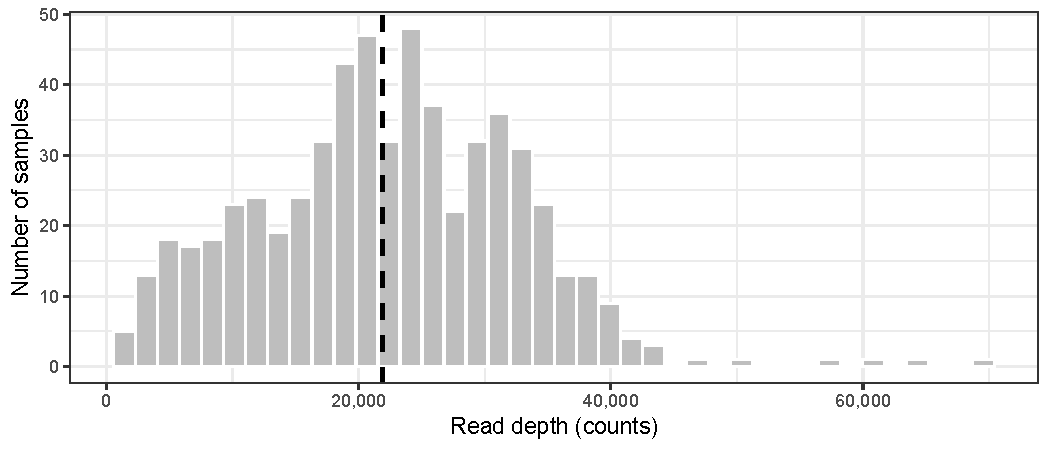
\includegraphics[width=\textwidth]{../ch07_application/figures/01_overview/thesis_seq_depth-1.pdf}
\caption{\textbf{Per-sample sequencing depth.} Distribution of sequencing depth across samples in the reduced PASTURE data set. The histogram shows the number of samples per read depth, with a median library size of 21{,}914 reads (dashed line) and a range from 1{,}456 to 69{,}556 reads.}
\label{fig:7app:library_size}
\end{figure}

%====================================
\subsection{Taxonomic aggregation and prevalence filtering}
\label{sec:7app:taxonomic_aggregation_filtering}
%====================================

After restricting the data set to the reduced analysis subset, ASVs with zero total counts within this subset are removed. Such ASVs occur only in samples outside the reduced data set and therefore do not provide information for the analyses in this chapter. At the ASV level, the original data set contains $p = 5834$ taxa, of which $p = 2045$ have at least one positive count in the reduced analysis subset.

The prevalence--abundance relationship at ASV level is shown in Figure~\ref{fig:7app:prevalence_abundance}. Most ASVs are observed in only a small fraction of samples, whereas a small number of taxa are both highly prevalent and abundant. This pattern is typical for infant gut microbiome data and illustrates why taxonomic aggregation and prevalence filtering are relevant preprocessing steps for the subsequent analyses. Low-prevalence taxa contribute strongly to sparsity, increase the influence of zero handling, and provide limited information for stable statistical estimation.

\begin{figure}[H]
\centering
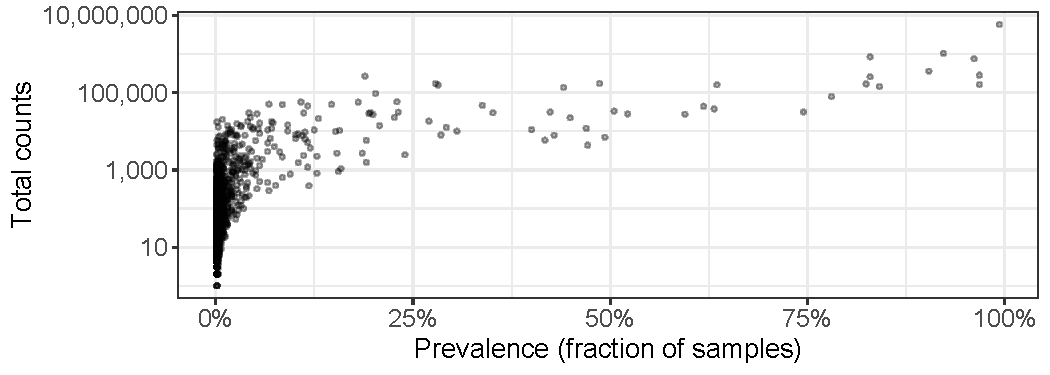
\includegraphics[width=\textwidth]{../ch07_application/figures/02_filtering/thesis_prevalence_asv-1.pdf}
\caption{\textbf{Prevalence--abundance relationship.} Each dot represents an amplicon sequence variant (ASV). The x-axis shows the proportion of samples in which the ASV is observed, i.e. has non-zero counts, and the y-axis shows the total number of counts across all samples. The y-axis is displayed on a log scale, while the axis labels correspond to the original count values.}
\label{fig:7app:prevalence_abundance}
\end{figure}

Table~\ref{tab:7app:taxonomic_overview} summarizes the number of taxa and the proportion of zero entries obtained at different taxonomic levels after restricting the data to the reduced analysis subset. As expected, aggregation to higher taxonomic ranks reduces both dimensionality and sparsity. However, aggregation also changes the biological and statistical target: an ASV-level feature represents an individual sequence variant, whereas a genus-level feature represents the combined signal of all ASVs assigned to the same genus.

\begin{table}[!ht]
\centering
\caption{\textbf{Number of taxa across taxonomic levels.} Number of taxa and proportion of zero entries obtained at different taxonomic levels after restricting the data to the reduced analysis subset and removing taxa with zero total counts.}
\label{tab:7app:taxonomic_overview}
\vspace{0.5em}
\begin{tabular}{lrr}
\toprule
Taxonomic level & Number of taxa & Zero entries (\%) \\
\midrule
ASV & 2045 & 98.2 \\
Genus & 235 & 89.7 \\
Family & 91 & 80.8 \\
Order & 52 & 73.8 \\
Class & 16 & 55.4 \\
Phylum & 10 & 54.9 \\
\bottomrule
\end{tabular}
\end{table}

All analyses in this application chapter are conducted at genus level unless stated otherwise. The ASV count table is therefore aggregated by summing counts over ASVs assigned to the same genus. The genus level provides a compromise between biological resolution, interpretability, and statistical stability: it is less sparse than the ASV-level table, but still sufficiently resolved to describe differences in the early-life gut microbiome at an interpretable taxonomic scale. The resulting unfiltered genus-level table contains $p = 235$ genera and is used for descriptive genus-level summaries and for the alpha diversity analysis.

At the genus level, the data are dominated by a small number of highly abundant taxa (Table~\ref{tab:7app:top_genera}). The most abundant genus is \emph{Bifidobacterium}, which is present in all samples and accounts for a large fraction of the mean relative abundance. Other prevalent genera include \emph{Escherichia-Shigella}, \emph{Streptococcus}, \emph{Bacteroides}, \emph{Enterococcus}, \emph{Blautia}, and a genus of the \emph{Enterobacteriaceae} family. These observations are consistent with previous studies on early-life gut microbiome development \citep{favier2003development}.

\begin{table}[!ht]
\centering
\caption{\textbf{Most abundant genera.} Top 10 most abundant genera in the reduced PASTURE data set ranked by mean relative abundance across samples before prevalence filtering. For each genus, the mean relative abundance, defined as the average proportion of counts assigned to a genus across samples, and the prevalence, defined as the proportion of samples in which the genus is observed, are reported.}
\label{tab:7app:top_genera}
\vspace{0.5em}
\begin{tabular}{lrr}
\toprule
Genus & Mean rel. abundance (\%) & Prevalence (\%) \\
\midrule
\emph{Bifidobacterium} & 63.8 & 100.0 \\
\emph{Escherichia-Shigella} & 5.9 & 97.3 \\
\emph{Streptococcus} & 4.9 & 99.3 \\
\emph{Bacteroides} & 4.6 & 90.5 \\
\emph{Enterobacteriaceae(F)} & 2.9 & 73.8 \\
\emph{Enterococcus} & 2.8 & 90.2 \\
\emph{[Ruminococcus] gnavus group} & 2.3 & 97.6 \\
\emph{Blautia} & 2.0 & 99.2 \\
\emph{Collinsella} & 1.3 & 85.0 \\
\emph{Lactobacillus} & 1.3 & 54.2 \\
\bottomrule
\end{tabular}
\end{table}

For all analyses except alpha diversity, an additional prevalence filter is applied at genus level. Genera observed in less than 1\% of the samples are removed. This threshold removes genera with too few non-zero observations to support stable statistical estimation, while retaining a broad genus-level representation of the microbiome. Table~\ref{tab:7app:prevalence_filtering} summarizes the effect of different prevalence thresholds on the number of retained genera and the proportion of zero entries. The 1\% filter reduces the number of genera from 235 to 117 and decreases the proportion of zero entries from 89.7\% to 79.6\%. More stringent thresholds would further reduce sparsity, but would also remove a large fraction of genera and thereby substantially narrow the taxonomic scope of the subsequent analyses.

\begin{table}[!ht]
\centering
\caption{\textbf{Effect of prevalence filtering on the genus-level count table.} Number of retained genera and proportion of zero entries for different prevalence thresholds. Prevalence is defined as the proportion of samples in which a genus has positive counts.}
\label{tab:7app:prevalence_filtering}
\vspace{0.5em}
\begin{tabular}{lrr}
\toprule
Prevalence threshold & Number of genera & Zero entries (\%) \\
\midrule
No prevalence filtering & 235 & 89.7 \\
$\geq 1\%$ of samples & 117 & 79.6 \\
$\geq 5\%$ of samples & 58 & 61.3 \\
$\geq 10\%$ of samples & 41 & 48.4 \\
$\geq 20\%$ of samples & 31 & 36.4 \\
\bottomrule
\end{tabular}
\end{table}

Although the 1\% prevalence filter reduces the overall proportion of zero entries, the retained genus-level table remains strongly sparse. Figure~\ref{fig:7app:zero_fraction_filtered_genera} shows the distribution of zero fractions across the 117 retained genera. Many genera are still absent from a large majority of samples, with a pronounced accumulation of zero fractions above 90\%. Thus, the filter removes only the most extremely rare genera and does not eliminate the need for zero-aware preprocessing and analysis methods in the subsequent sections.


\begin{figure}[!htb]
\centering
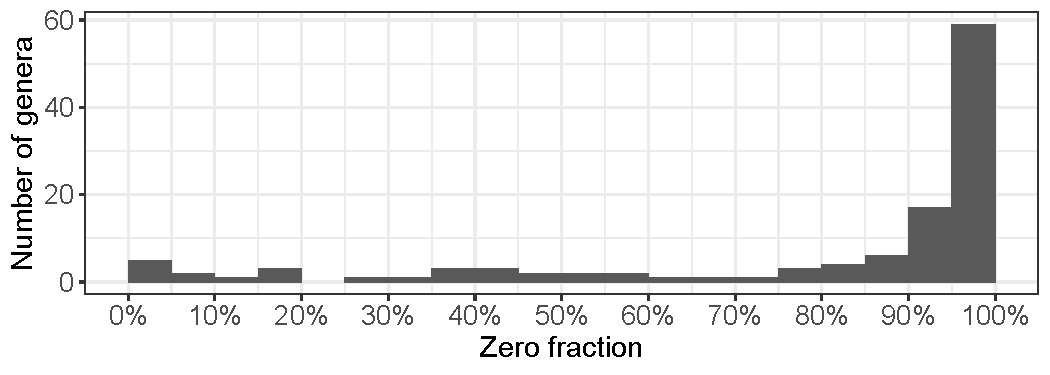
\includegraphics[width=0.75\textwidth]{../ch07_application/figures/02_filtering/thesis_zero_fraction_plot-1.pdf}
\caption{\textbf{Distribution of zero fractions after 1\% prevalence filtering.} The histogram shows, for each of the 117 genera retained after applying the 1\% prevalence filter, the proportion of samples with zero counts.}
\label{fig:7app:zero_fraction_filtered_genera}
\end{figure}

%====================================
\subsection{Default data set for downstream analyses}
\label{sec:7app:default_data}
%====================================

The downstream analyses in this chapter use the genus-level representation introduced in Section~\ref{sec:7app:taxonomic_aggregation_filtering}. Unless stated otherwise, analyses after the within-sample diversity section are based on the $1\%$ prevalence-filtered genus-level count table with $117$ retained genera. This table is referred to as the default analysis data set in the following sections. The main exception is the within-sample diversity analysis, which is computed before prevalence filtering because removing low-prevalence genera would directly change the target of richness and diversity estimation. If another taxonomic table, sample subset, or data transformation is used in a later section, this is stated explicitly.

The default analysis data set is represented on different scales depending on the analysis target. The choice of representation follows the preprocessing strategy summarized in Section~\ref{sec:2micro:preprocessing_choices_thesis} and is implemented here for the reduced PASTURE data set. Relative abundances are used for descriptive summaries and for analyses based on Bray--Curtis dissimilarity, because they provide an interpretable representation of the observed sample composition after adjustment for library size. For analyses requiring a log-ratio representation, counts are first converted to relative abundances, zeros are replaced by multiplicative replacement, and the resulting strictly positive compositions are transformed using the centered log-ratio transformation. This CLR representation is used for Aitchison distances, regression models for compositional responses, compositional equivalence, exploratory CLR-coordinate visualizations, the CLR-based part of the differential distribution analysis, and network analyses.

Analyses based on EBF duration require an additional distinction. When EBF duration is used as the main binary grouping variable, samples with missing EBF duration and the three samples in the sparse 1-month EBF category are excluded from the corresponding two-group comparison. The resulting contrast compares children without EBF ($n=179$) with children with EBF duration $\ge 2$ months ($n=375$). This exclusion is applied only in analyses that explicitly use this binary EBF contrast and is not a general filtering step applied to the entire chapter. To improve readability, the EBF duration $\geq 2$ months group is referred to as the ``EBF'' group and the EBF duration $=0$ months group as the ``non-EBF'' group in the following comparative analyses.

Figure~\ref{fig:7app:rel-clr-histogram-comparison} illustrates the effect of the relative-abundance and CLR representations for the most abundant genera. The left panels show relative abundances, which are bounded between zero and one and are often strongly concentrated near zero for sparse genera. The right panels show the corresponding CLR coordinates after multiplicative replacement. These values are no longer abundances in the original sense, but log-ratio coordinates relative to the sample-wise geometric mean. Originally zero observations are mapped to low CLR values whose location depends on the replacement rule and on the remaining composition of the same sample. The comparison emphasizes that downstream analyses based on CLR-transformed data operate in a different coordinate system and should be interpreted in terms of relative log-ratios rather than absolute microbial abundance.

\begin{figure}[!htb]
\centering
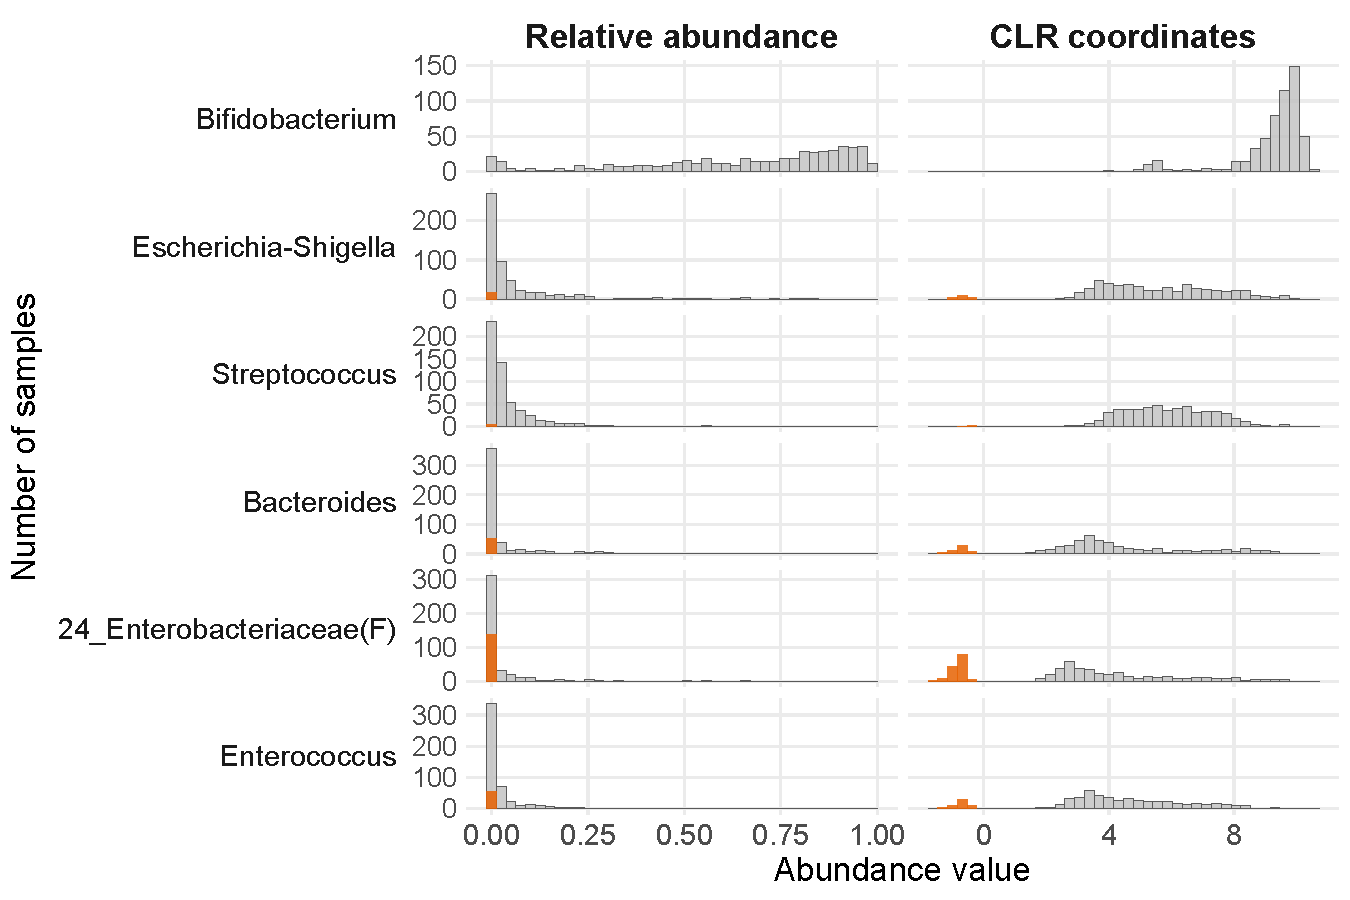
\includegraphics[width=\textwidth]{../ch07_application/figures/07_exploration/thesis_rel_to_clr_histogram_comparison-1.pdf}
\caption{\textbf{Relative abundances and CLR coordinates for the most abundant genera.} The left panels show relative abundances after total sum scaling, and the right panels show CLR coordinates after multiplicative replacement of zeros. Orange bars indicate samples in which the corresponding genus was originally absent before zero replacement. The figure illustrates that CLR transformation changes the coordinate representation of the data: values are interpreted as log-ratios relative to the sample-wise geometric mean and not as absolute abundances.}
\label{fig:7app:rel-clr-histogram-comparison}
\end{figure}

Taken together, the reduced data set retains the central statistical characteristics of microbiome sequencing data: unequal library sizes, compositional constraints, sparsity, and strong heterogeneity in taxon prevalence and abundance. The default genus-level analysis data set provides a common basis for the following sections, while deviations in taxonomic resolution, sample subset, or data representation are stated where they are required by the respective method. This structure supports a coherent analysis workflow from community-level exploration to feature-level testing and network-based comparison.

%%%%%%%%%%%%%%%%%%%%%%%%%%%%%%%%%%%%%
\section{Within-sample diversity}
\label{sec:7app:alpha}
%%%%%%%%%%%%%%%%%%%%%%%%%%%%%%%%%%%%%

Within-sample diversity, commonly referred to as \emph{alpha diversity}, provides a first aggregated view of microbial community structure by reducing each sample-specific taxon profile to a scalar summary. As introduced in Section~\ref{sec:3community:within_sample_div}, it can be characterized by richness, which reflects the number of taxa present in a sample, and by diversity indices such as Shannon entropy and the Gini--Simpson index, which additionally account for the distribution of abundances across taxa.

In this section, within-sample diversity in the reduced PASTURE data set is analyzed using the model-based estimators described in Chapter~\ref{ch:community}. We first compare classical and model-based richness estimates and assess their dependence on sequencing depth. We then investigate differences in diversity across cohort variables using rank-based tests.
To assess the robustness of these findings, asymptotic and permutation-based $p$-values are compared, including $p$-value refinement with the \texttt{permApprox} framework introduced in Chapter~\ref{ch:permapprox}. Finally, regression-based diversity models are used to incorporate covariates directly into the diversity estimation framework and to compare adjusted effects with the unadjusted group-wise analyses.

%====================================
\subsection{Analysis data}
\label{sec:7app:alpha:data}
%====================================

As stated in Section~\ref{sec:7app:default_data}, within-sample diversity is the main analysis in this chapter that is computed before prevalence filtering. All analyses in this section are therefore based on the unfiltered genus-level count table introduced in Section~\ref{sec:7app:taxonomic_aggregation_filtering}, comprising $592$ samples and $235$ genera. The additional $1\%$ prevalence filter used as the default in later sections is not applied here, because removing low-prevalence genera would directly change the target of richness and diversity estimation.

Although within-sample diversity is often computed at the ASV level, the analysis is performed at the genus level to maintain the taxonomic resolution used throughout the application chapter and to reduce the computational burden of model-based diversity estimation. The exploratory group-wise analyses consider all cohort variables summarized in Section~\ref{sec:7app:data}, including country, sex, mode of delivery, breastfeeding-related variables, prenatal smoking, and number of siblings.

As discussed in Chapter~\ref{ch:community}, rarefaction is not used as a preprocessing step. Instead, richness and diversity are estimated using the model-based approaches proposed by \citet{willis2018divnet,willis2022breakaway}, which account for sampling effort and uncertainty due to unobserved taxa. Consequently, no additional rarefaction, normalization, or prevalence filtering is applied to the count data in this section.

%====================================
\subsection{Comparison of richness estimators}
\label{sec:7app:alpha:rich_comparison}
%====================================

We compare three conceptually distinct notions of richness: (i) observed richness, defined as the number of detected genera per sample, (ii) sample-wise richness estimates obtained using the \texttt{breakaway} package \citep{willis2022breakaway} without covariates, and (iii) model-based richness predictions with \texttt{breakaway}, which are obtained from a regression model that incorporates covariates.

Observed richness is a purely empirical quantity that counts the number of non-zero taxa in each sample. As such, it is directly influenced by sequencing depth and does not account for unobserved low-abundance taxa (cf. Section~\ref{sec:3community:within:richness}). In contrast, \texttt{breakaway} estimates the total richness of a sample by extrapolating from the frequency count table, thereby correcting for taxa that are present but not observed. Importantly, when applied without covariates, \texttt{breakaway} produces \emph{independent, sample-wise estimates} that do not borrow information across samples.

Figure~\ref{fig:7app:alpha_obs_vs_breakaway} (left panel) compares observed richness to \texttt{breakaway} estimates obtained without covariates. The two measures are almost perfectly linearly related, indicating that the correction for unobserved taxa is negligible in this data set. Consequently, \texttt{breakaway} does not substantially alter the ranking of samples compared to observed richness. Similar results are obtained at the ASV level (not shown), suggesting that this behavior is not driven by the level of taxonomic aggregation.

\begin{figure}[H]
    \centering
    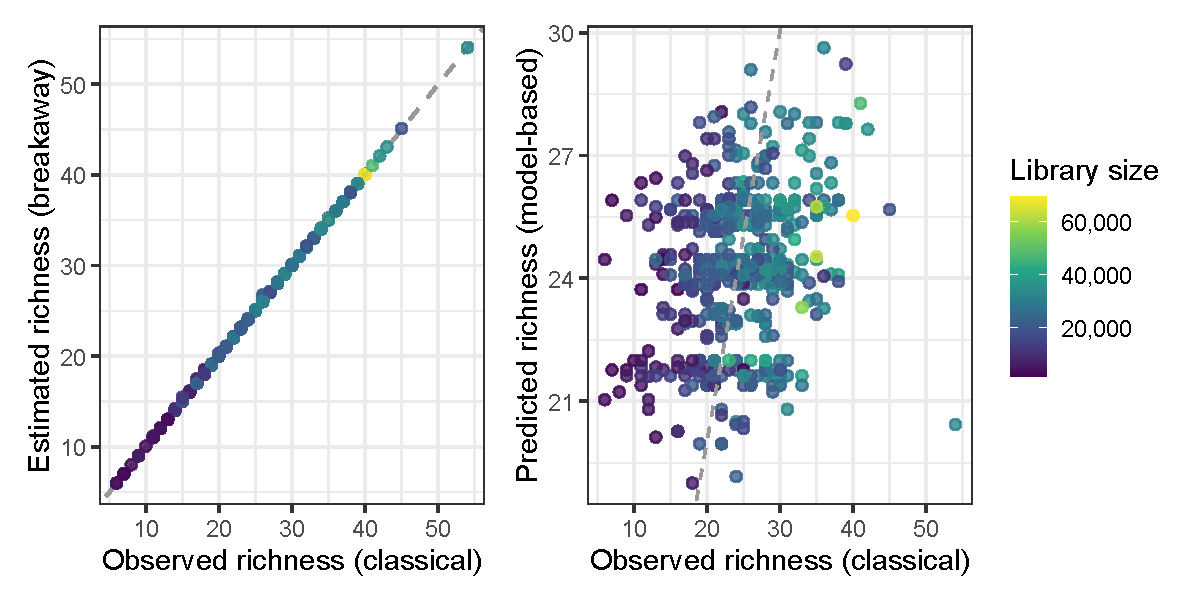
\includegraphics[width=\textwidth]{../ch07_application/figures/03_alpha_diversity/thesis_observed_vs_predicted_richness_libsize_combined-1.pdf}
    \caption{\textbf{Comparison of observed and model-based richness.} Left: observed richness versus \texttt{breakaway} estimates obtained without covariates. Right: observed richness versus model-based predicted richness obtained from a \texttt{breakaway} regression model with covariates. Points are colored by library size.}
    \label{fig:7app:alpha_obs_vs_breakaway}
\end{figure}

To understand this behavior, it is instructive to examine the frequency count structure underlying the breakaway estimator. Breakaway relies on the number of rare taxa, in particular singletons (taxa observed exactly once), to estimate the number of unobserved taxa. Figure~\ref{fig:7app:alpha_frequency_counts} shows the mean number of taxa per sample as a function of their observed frequency. Notably, the number of singletons is exactly zero across samples. As a consequence, the ratio-based estimators used by breakaway collapse to the observed richness, since the observed frequency count spectrum provides little information for estimating unobserved taxa. This explains the near identity between observed and breakaway richness in Figure~\ref{fig:7app:alpha_obs_vs_breakaway}.

The absence of singletons was observed not only at the genus level but also at the ASV level (not shown). Since singleton ASVs are commonly removed during denoising and error-correction procedures in amplicon sequence processing pipelines such as DADA2, this pattern is likely a consequence of the preprocessing applied to the sequencing data prior to the present analysis. As a result, the frequency count spectrum contains little information for extrapolating beyond the observed richness.

\begin{figure}[H]
    \centering
    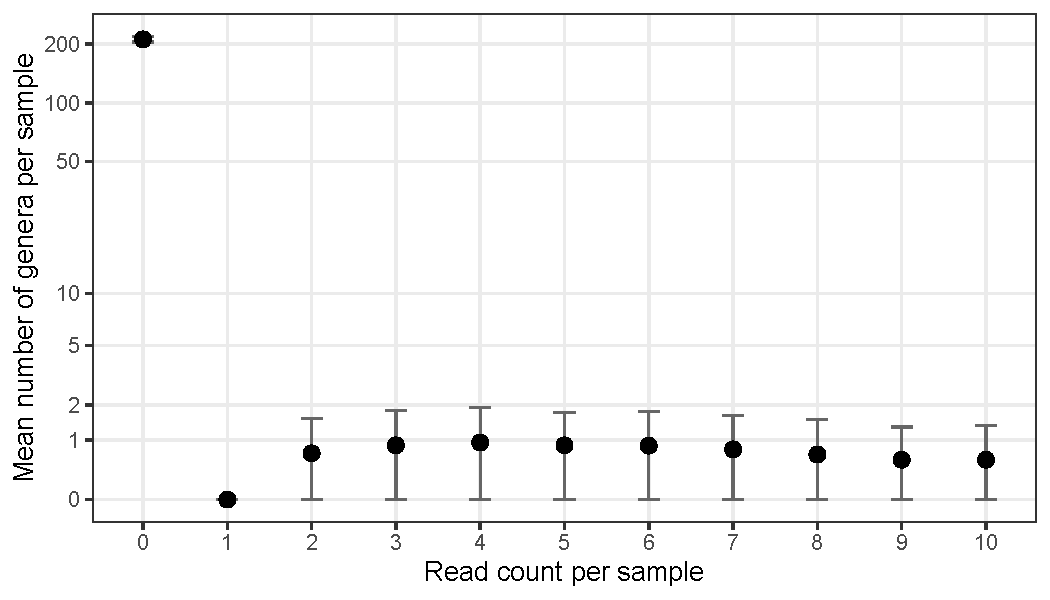
\includegraphics[width=0.9\textwidth]{../ch07_application/figures/03_alpha_diversity/thesis_freq_spectrum_genus-1.pdf}
    \caption{\textbf{Frequency count spectrum at genus level.} Mean number of genera per sample as a function of their observed frequency (read count per sample). Error bars indicate variability across samples. The absence of singletons (genera with one read count per sample) implies that no information about unobserved taxa is available for ratio-based richness estimation.}
    \label{fig:7app:alpha_frequency_counts}
\end{figure}

In a second step, richness is modeled as a function of covariates using the \texttt{betta()} function from \texttt{breakaway}. In contrast to the sample-wise estimation described above, this model is fitted across samples and yields \emph{predicted richness values} conditional on the covariates. These values therefore represent fitted expectations under the model rather than direct estimates of sample-specific richness.

The effect of this modeling step is illustrated in Figure~\ref{fig:7app:alpha_obs_vs_breakaway} (right panel). Compared to the near one-to-one relationship in the left panel, the predicted richness values exhibit substantially reduced variability and a compressed range. This behavior reflects the fact that regression-based predictions are shrunk towards the fitted mean structure and primarily capture systematic variation explained by the covariates. As a consequence, they no longer preserve the original between-sample variability present in the data.

This distinction is crucial for interpretation. While \texttt{breakaway} without covariates aims to estimate the underlying richness of each individual sample, the regression model targets the expected richness given the covariates. The resulting quantities therefore answer different statistical questions: one is a per-sample estimate, the other a model-based prediction.

For comparative analyses, this difference has direct methodological implications. Using model-based predicted richness for group comparisons would lead to circular inference, as the grouping variable is already used in the model fitting step. Any subsequent test would therefore assess differences that have been, at least partially, imposed by the model itself. To avoid this double use of information, all statistical comparisons in the following are based on the sample-wise richness estimates rather than on model-based predictions.

Model-based predictions nevertheless serve an important role for visualization and interpretation of covariate effects. They provide a smoothed representation of systematic trends and can help disentangle the influence of multiple covariates. However, they are not suitable as input for hypothesis testing in this setting.

Taken together, these results highlight two key points. First, at the genus level, the correction for unobserved taxa provided by breakaway has only a minor effect when applied without covariates. This is not merely an empirical observation but can be directly explained by the absence of singletons in the data, which eliminates the information required for extrapolation. Second, regression-based modeling substantially alters the scale and variability of richness by imposing a covariate-driven structure, which makes the resulting predictions fundamentally different from sample-wise richness estimates.

%====================================
\subsection{Within-sample diversity across cohort variables}
\label{sec:7app:alpha:diversity_measures}
%====================================

In addition to richness, we considered two complementary diversity indices that account for the distribution of abundances within samples: the Shannon index and the Gini--Simpson index. Both measures were estimated using the \texttt{DivNet} framework described in Section~\ref{sec:3community:within_sample_div}, which provides model-based diversity estimates while accounting for compositional dependencies among taxa. The \texttt{divnet()} function from the \texttt{DivNet} package \citep{willis2018divnet} was applied to the genus-level count table to estimate Shannon and Simpson diversity. For the log-ratio representation underlying the model, \textit{Bifidobacterium} was used as the reference taxon, as it exhibited 100\% prevalence across all samples. The Simpson index returned by \texttt{DivNet} was transformed into the Gini--Simpson index by computing $1 - \text{Simpson}$. While the Simpson index measures concentration or dominance, the Gini--Simpson index instead quantifies diversity, with larger values indicating a more even distribution of abundances across taxa.

To investigate whether within-sample diversity differs across cohort variables, we compared richness, Shannon diversity, and the Gini--Simpson index across all covariates available in the reduced data set: Country, Sex, C-section, BF duration, EBF duration, Smoking, and Siblings (Table~\ref{tab:7app:sample_characteristics}). For EBF duration, the three samples in the one-month category were excluded from the group comparison, because this category was too small to support an informative comparison. For each variable and diversity measure, an overall group effect was first assessed using a Kruskal--Wallis test based on its standard asymptotic chi-squared approximation. If the resulting $p$-value was significant at the $\alpha = 0.05$ level and the variable had more than two groups, pairwise comparisons between groups were additionally performed using asymptotic Wilcoxon rank-sum tests.

The resulting overall test statistics and asymptotic $p$-values are summarized in Table~\ref{tab:7app:perm_results}. Pairwise Wilcoxon results are not included in the table, but significant pairwise comparisons are annotated in the corresponding figures. Figure~\ref{fig:7app:alpha_div_excl_bf} shows the selected EBF duration comparison, while additional visualizations for the remaining cohort variables are provided in Appendix~\ref{sec:app:7app:alpha_remaining}, and also in the \href{https://github.com/stefpeschel/phd_thesis/tree/main/ch07_application}{\texttt{ch07\_application}} folder of the thesis repository described at the beginning of this chapter. The subsequent subsection evaluates whether the asymptotic $p$-values used for interpretation agree with permutation-based and \texttt{permApprox}-refined $p$-values.

The results indicate that within-sample diversity differs substantially across several cohort variables. In particular, BF duration, EBF duration, Smoking, and Country show significant associations with both diversity indices. In contrast, richness exhibits fewer significant associations and generally weaker effects, consistent with the findings of the previous subsection. Sex and Siblings do not show significant differences for any of the considered measures. For C-section, significant differences are observed for Shannon diversity and the Gini--Simpson index, whereas richness remains non-significant.

Among the considered variables, BF duration and EBF duration show the strongest associations with within-sample diversity, as reflected by the smallest asymptotic $p$-values in Table~\ref{tab:7app:perm_results}. These variables therefore represent promising candidates for further investigation and more detailed group comparisons in the subsequent sections.

For the downstream analyses, we aim to identify a grouping variable with two sufficiently large and balanced groups. In this regard, EBF duration provides a suitable choice. In particular, the comparison between the groups corresponding to no exclusive breastfeeding and at least two months of exclusive breastfeeding yields more balanced group sizes than the corresponding categorization based on BF duration (Table~\ref{tab:7app:sample_characteristics}).

Figure~\ref{fig:7app:alpha_div_excl_bf} shows the corresponding distributions of richness, Shannon diversity, and the Gini--Simpson index across the two EBF duration groups. While richness shows only minor differences between groups, both diversity indices indicate substantially lower diversity for at least two months of exclusive breastfeeding. The effect is particularly pronounced for the Shannon index, where the distributions are clearly shifted between groups. This pattern is in line with previous studies identifying infant feeding mode as a major determinant of early-life gut-microbiome composition and reporting lower gut microbial diversity among exclusively breastfed infants during early infancy \citep{ho2018metaanalysis,ma2020comparison,odiase2023gut}.

\begin{figure}[H]
\centering
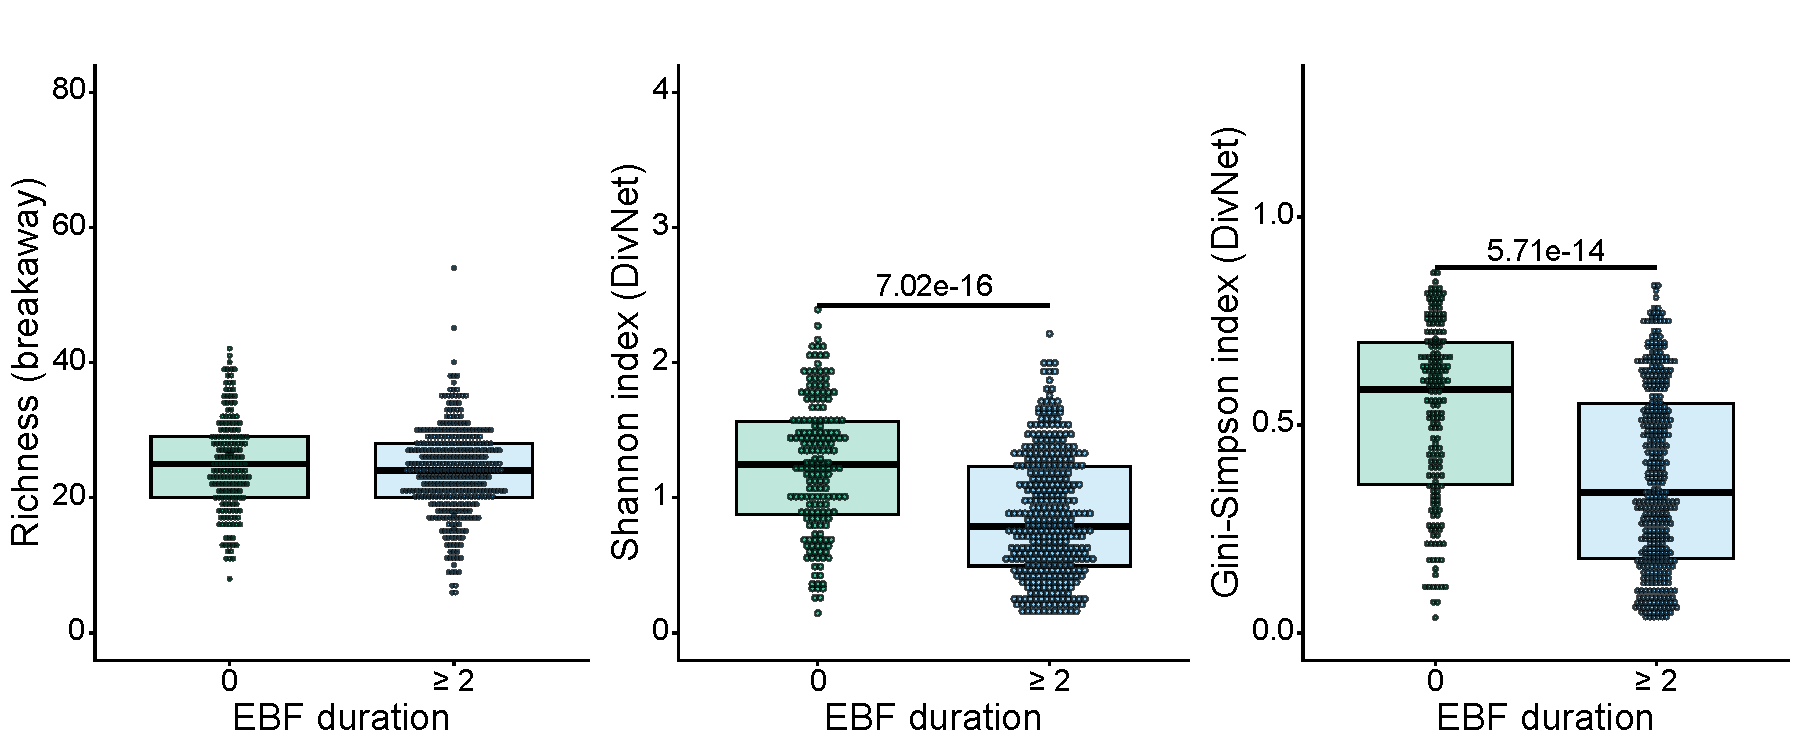
\includegraphics[width=\textwidth]{../ch07_application/figures/03_alpha_diversity/thesis_breast_excl_2m-1.pdf}
\caption{\textbf{Within-sample diversity by EBF duration.} Sample-wise estimates of richness, Shannon diversity, and the Gini--Simpson index for children with no exclusive breastfeeding and children with at least two months of exclusive breastfeeding. Richness was estimated using \texttt{breakaway}; Shannon diversity and the Gini--Simpson index were estimated using \texttt{DivNet}. Reported $p$-values are asymptotic Kruskal--Wallis $p$-values. The one-month category was excluded because it contained only three samples. Sample sizes are 179 for no exclusive breastfeeding and 375 for at least two months of exclusive breastfeeding.}
\label{fig:7app:alpha_div_excl_bf}
\end{figure}

%====================================
\subsection{Permutation-based inference and $p$-value refinement}
\label{sec:7app:alpha:permutation}
%====================================

The previous subsection relied on the standard asymptotic approximation of the Kruskal--Wallis test statistic, where the test statistic is approximated by a chi-squared distribution with degrees of freedom equal to the number of groups minus one. While this approximation is commonly used in practice, its validity may be affected by small or unbalanced group sizes, ties in the data, and deviations from the asymptotic regime. To assess the robustness of the obtained results, we therefore complemented the asymptotic inference by permutation-based testing.

For each cohort variable and diversity measure, the Kruskal--Wallis test statistic was recomputed under random permutations of the group labels to generate an empirical null distribution for the overall group effect. The test statistic was computed directly from the group-wise rank sums using the formulation introduced in Section~\ref{sec:3community:within:testing}. Permutation-based $p$-values were then computed from the number of permuted statistics greater than or equal to the observed statistic using the adjusted estimator in Equation~\eqref{eq:6perm:empirical_pvalue}. The comparison in this subsection focuses on the overall tests reported in Table~\ref{tab:7app:perm_results}. The pairwise Wilcoxon annotations shown in Figure~\ref{fig:7app:alpha_div_excl_bf} and Appendix~\ref{sec:app:7app:alpha_remaining} are based on asymptotic Wilcoxon rank-sum tests.

Although substantially fewer permutations would have been sufficient for the present analysis, we generated $10^6$ permutations for each overall test. In this setting, the computational cost of permutation testing is comparatively small because the within-sample diversity measures are computed only once and each permutation merely requires recomputation of the rank-based test statistic. The large number of permutations therefore provides an opportunity to directly assess how closely the asymptotic $p$-values agree with the empirical permutation distribution over several orders of magnitude.

The resulting $p$-values are summarized in Table~\ref{tab:7app:perm_results}. Overall, the empirical permutation $p$-values closely match the asymptotic $p$-values and typically agree up to the same order of magnitude, even for very small $p$-values. This close agreement provides reassurance that the asymptotic approximation yields similar inferential conclusions in the present setting. Thus, permutation-based inference does not appear to be necessary for obtaining materially different conclusions for these overall diversity tests.

Nevertheless, this setting provides a useful opportunity to evaluate the behavior of the \texttt{permApprox} framework in a low-dimensional setting. The empirical permutation $p$-values are bounded below by about $10^{-6}$ due to the finite number of permutations, whereas \texttt{permApprox} further refines the tail probabilities by fitting a generalized Pareto distribution to the upper tail of the permutation distribution under the support constraint proposed in Section~\ref{sec:6perm:constraint}. The refinement was performed using the default settings of the package, except that the number of starting exceedances was reduced to 5000 permutations (corresponding to 0.5\% of all permutations) to reduce runtime.

The refined $p$-values shown in the rightmost columns of Table~\ref{tab:7app:perm_results} remain close to the asymptotic $p$-values and are slightly more conservative for extremely small $p$-values. This behavior is desirable, as it avoids overly optimistic tail extrapolation while still extending the resolution beyond the empirical permutation limit. In the present analysis, the refinement does not alter the resulting significance decisions, which is expected given the close agreement between asymptotic and empirical permutation inference.

These results illustrate an important practical aspect of the proposed methodology. In the present setting, the asymptotic approximation already provides reliable inference, likely due to the comparatively large sample size and the absence of severe violations of the assumptions underlying the rank-based tests. In settings where these assumptions are less well satisfied, for example in the presence of smaller sample sizes, strongly imbalanced groups, or more irregular null distributions, permutation-based inference provides a robust alternative that does not rely on parametric approximations. In such cases, \texttt{permApprox} becomes particularly useful by refining extremely small empirical permutation $p$-values beyond the finite permutation resolution. As will be demonstrated in the subsequent sections, this refinement becomes increasingly relevant in more complex testing scenarios involving large-scale multiple testing and computationally expensive permutation procedures.


\begin{table}[H]
\centering
\caption{Kruskal--Wallis test results for within-sample diversity across cohort variables. $H$ is the Kruskal--Wallis test statistic. Richness was estimated using \texttt{breakaway}; Shannon and Gini--Simpson diversity were estimated using \texttt{DivNet}. $p$ (asymptotic) denotes the chi-squared approximation used for the exploratory interpretation; $p$ (permutation) denotes empirical permutation $p$-values based on $10^6$ permutations; $p$ (GPD-refined) denotes $p$-values obtained with \texttt{permApprox} for small empirical permutation $p$-values. $p$-values are rounded and shown in scientific notation with two digits after the decimal point. The smallest attainable empirical permutation $p$-value is $1/(10^6+1)$, which is displayed as $1.00\mathrm{e}{-06}$ after rounding.}
\label{tab:7app:perm_results}
\centering
\begin{threeparttable}
\begin{tabular}[t]{l@{\hspace{4em}}rlll}
\toprule
Measure & $H$ & $p$ (asymptotic) & $p$ (permutation) & $p$ (GPD-refined)\\
\midrule
\addlinespace[0.3em]
\multicolumn{5}{l}{\textbf{Country}}\\
\hspace{1em}Richness & 31.57 & 1.40e-07$^{***}$ & 1.00e-06$^{***}$ & 1.99e-07$^{***}$\\
\hspace{1em}Shannon & 40.06 & 2.00e-09$^{***}$ & 1.00e-06$^{***}$ & 3.01e-09$^{***}$\\
\hspace{1em}Gini-Simpson & 39.88 & 2.19e-09$^{***}$ & 1.00e-06$^{***}$ & 4.89e-09$^{***}$\\
\addlinespace[0.3em]
\multicolumn{5}{l}{\textbf{Sex}}\\
\hspace{1em}Richness & 1.79 & 1.80e-01 & 1.77e-01 & 1.77e-01\\
\hspace{1em}Shannon & 1.85 & 1.73e-01 & 1.72e-01 & 1.72e-01\\
\hspace{1em}Gini-Simpson & 2.10 & 1.47e-01 & 1.49e-01 & 1.49e-01\\
\addlinespace[0.3em]
\multicolumn{5}{l}{\textbf{C-section}}\\
\hspace{1em}Richness & 0.33 & 5.64e-01 & 5.64e-01 & 5.64e-01\\
\hspace{1em}Shannon & 4.86 & 2.74e-02$^{*}$ & 2.54e-02$^{*}$ & 2.50e-02$^{*}$\\
\hspace{1em}Gini-Simpson & 5.73 & 1.67e-02$^{*}$ & 1.35e-02$^{*}$ & 1.43e-02$^{*}$\\
\addlinespace[0.3em]
\multicolumn{5}{l}{\textbf{BF duration}}\\
\hspace{1em}Richness & 7.69 & 2.14e-02$^{*}$ & 2.12e-02$^{*}$ & 2.12e-02$^{*}$\\
\hspace{1em}Shannon & 83.47 & 7.51e-19$^{***}$ & 1.00e-06$^{***}$ & 1.44e-17$^{***}$\\
\hspace{1em}Gini-Simpson & 73.49 & 1.10e-16$^{***}$ & 1.00e-06$^{***}$ & 4.69e-15$^{***}$\\
\addlinespace[0.3em]
\multicolumn{5}{l}{\textbf{EBF duration}}\\
\hspace{1em}Richness & 2.73 & 9.84e-02$^{.}$ & 9.84e-02$^{.}$ & 9.84e-02$^{.}$\\
\hspace{1em}Shannon & 65.13 & 7.02e-16$^{***}$ & 1.00e-06$^{***}$ & 5.18e-14$^{***}$\\
\hspace{1em}Gini-Simpson & 56.47 & 5.71e-14$^{***}$ & 1.00e-06$^{***}$ & 5.04e-14$^{***}$\\
\addlinespace[0.3em]
\multicolumn{5}{l}{\textbf{Smoking}}\\
\hspace{1em}Richness & 3.95 & 4.70e-02$^{*}$ & 4.69e-02$^{*}$ & 4.69e-02$^{*}$\\
\hspace{1em}Shannon & 18.81 & 1.45e-05$^{***}$ & 1.30e-05$^{***}$ & 1.01e-05$^{***}$\\
\hspace{1em}Gini-Simpson & 18.08 & 2.12e-05$^{***}$ & 1.60e-05$^{***}$ & 1.47e-05$^{***}$\\
\addlinespace[0.3em]
\multicolumn{5}{l}{\textbf{Siblings}}\\
\hspace{1em}Richness & 1.41 & 4.94e-01 & 4.97e-01 & 4.97e-01\\
\hspace{1em}Shannon & 2.66 & 2.64e-01 & 2.61e-01 & 2.61e-01\\
\hspace{1em}Gini-Simpson & 3.04 & 2.18e-01 & 2.20e-01 & 2.20e-01\\
\bottomrule
\end{tabular}
\begin{tablenotes}
\item $^{***}:p<0.001$; $^{**}:p<0.01$; $^{*}:p<0.05$; $^{\textbf{.}}:p<0.1$.
\end{tablenotes}
\end{threeparttable}
\end{table}

%====================================
\subsection{Regression-based within-sample diversity analysis}
\label{sec:7app:alpha:regression}
%====================================

As a complementary approach to the group-wise comparisons, we fitted regression-based alpha diversity models using the \texttt{betta()} function from the \texttt{breakaway} package. The same modeling framework was already used in Section~\ref{sec:7app:alpha:rich_comparison} to obtain covariate-based richness predictions. Here, we focus on the regression coefficients rather than the predicted values, since the aim is to assess which covariates remain associated with alpha diversity when all variables are considered jointly.

The \texttt{betta()} function takes diversity estimates together with their estimated standard errors as input and fits a regression model that accounts for uncertainty in the estimated response. We applied this approach separately to richness, Shannon diversity, and the Gini--Simpson index. For richness, we used the estimates and standard errors obtained from \texttt{breakaway}; for Shannon diversity and the Gini--Simpson index, we used the estimates and standard errors obtained from \texttt{DivNet}. The model included all covariates considered in the group-wise analyses, namely country, sex, mode of delivery, breastfeeding duration, exclusive breastfeeding duration, prenatal smoking, and number of siblings. Samples with missing values in any of these covariates were excluded from the regression analysis.

Figure~\ref{fig:7app:alpha_betta} summarizes the resulting coefficient estimates and corresponding 95\% confidence intervals. For categorical variables with more than two levels, the first category was used as reference level. Positive coefficients indicate higher expected diversity compared to the reference category, whereas negative coefficients indicate lower expected diversity after adjustment for the remaining covariates.

\begin{figure}[H]
    \centering
    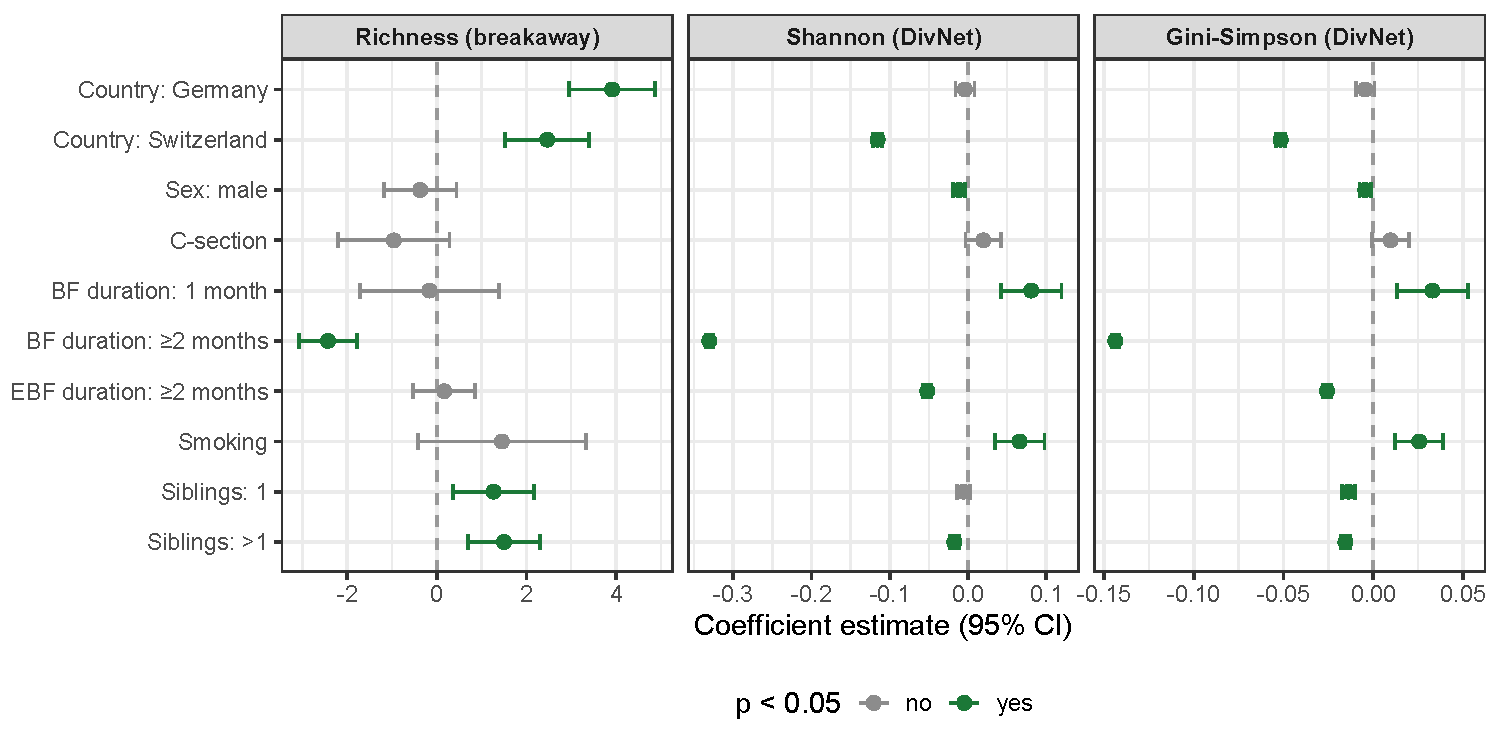
\includegraphics[width=\textwidth]{../ch07_application/figures/03_alpha_diversity/thesis_betta_forest_combined-1.pdf}
    \caption{Regression coefficients and corresponding 95\% confidence intervals obtained from the \texttt{betta()} models for richness, Shannon diversity, and the Gini--Simpson index. Green points indicate coefficients with $p < 0.05$.}
    \label{fig:7app:alpha_betta}
\end{figure}

Overall, the regression-based results are largely consistent with the group-wise comparisons summarized in Table~\ref{tab:7app:perm_results}. Breastfeeding-related variables, Smoking, and Country remain associated with alpha diversity after covariate adjustment. In particular, BF duration $\ge2$ months is associated with substantially lower richness, Shannon diversity, and Gini--Simpson diversity. EBF duration $\ge2$ months is also associated with lower Shannon and Gini--Simpson diversity, whereas its coefficient for richness is close to zero and not significant. This agrees with the group-wise comparisons, where EBF duration showed strong differences in diversity indices but not in richness. Because the two BF variables are closely related, the corresponding regression coefficients should be interpreted as conditional associations within the joint model rather than as independent marginal effects.

For Country, the regression model confirms differences in within-sample diversity, but the direction and magnitude depend on the measure considered. Compared to Austria (the reference country), Germany and Switzerland show higher richness, whereas Switzerland shows lower Shannon and Gini--Simpson diversity. This indicates that differences in richness and evenness do not necessarily point in the same direction, again emphasizing the importance of considering multiple diversity measures.

One notable discrepancy concerns the effect of C-section. In the marginal Kruskal--Wallis tests, both Shannon diversity and the Gini--Simpson index showed significant differences between delivery modes. In contrast, the corresponding regression coefficients are close to zero and no longer statistically significant.

To investigate this discrepancy further, Figure~\ref{fig:7app:alpha_csection_bf} compares BF duration distributions between delivery modes and additionally stratifies Shannon diversity by both variables. The left panel shows that vaginally delivered infants are more frequently represented in the long BF category, which is associated with lower diversity. The stratified boxplots in the right panel indicate that within BF strata, differences between delivery modes are substantially reduced, especially in the ``$\ge$ 2 months'' group, which contains the majority of the samples. This suggests that the apparent delivery mode effect observed in the unconditioned group comparisons is at least partly explained by differences in BF behavior.

This comparison illustrates the different targets of the two inferential strategies. The Kruskal--Wallis test assesses marginal group differences separately for each covariate, whereas the \texttt{betta()} models estimate associations conditioned on the remaining variables. The two approaches therefore answer related but not identical questions. In the present analysis, they lead to largely consistent conclusions, with the exception of delivery mode, where the regression model suggests that the marginal association is confounded by breast feeding duration.

\begin{figure}[H]
	\centering
	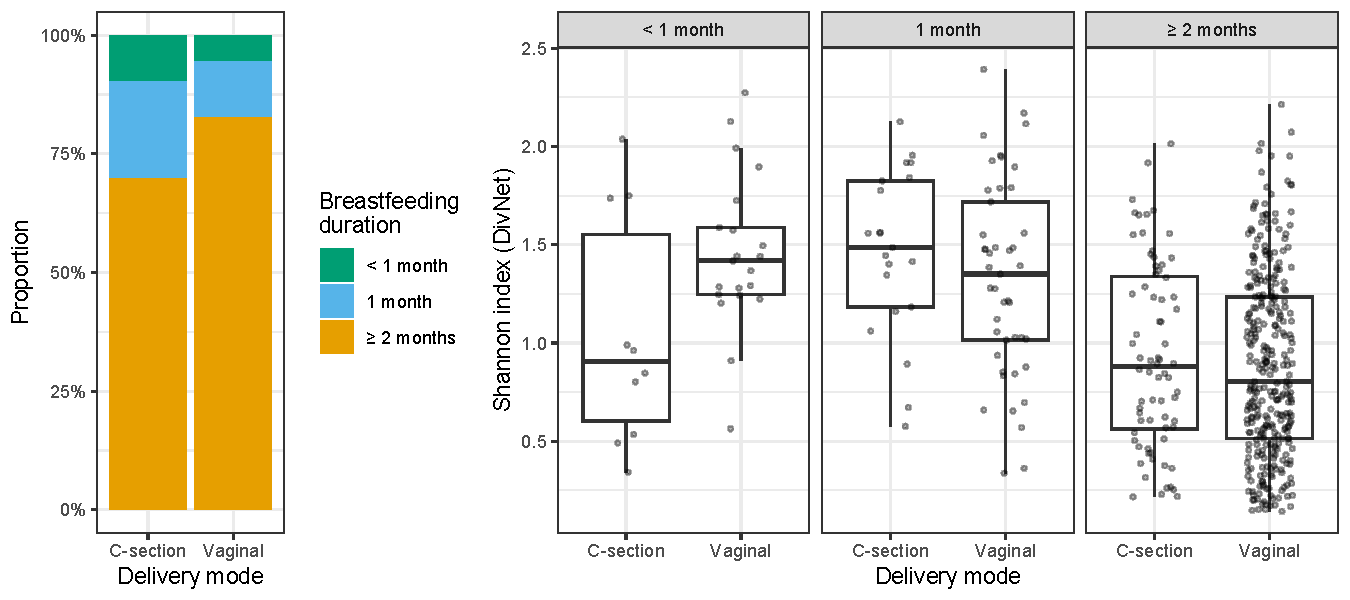
\includegraphics[width=\textwidth]{../ch07_application/figures/03_alpha_diversity/thesis_cesarean_breastfeed_confounding-1.pdf}
	\caption{\textbf{Diagnostic plots to investigate the effect of C-section.} Left: distribution of BF duration across delivery modes. Right: Shannon diversity stratified by BF duration and delivery mode. The apparent association between delivery mode and alpha diversity is reduced after accounting for BF duration.}
	\label{fig:7app:alpha_csection_bf}
\end{figure}

%%%%%%%%%%%%%%%%%%%%%%%%%%%%%%%%%%%%%
\section{Between-sample dissimilarity}
\label{sec:7app:beta}
%%%%%%%%%%%%%%%%%%%%%%%%%%%%%%%%%%%%%

The preceding within-sample diversity analyses summarized each sample by a single diversity value. We now turn to between-sample dissimilarity, which compares microbial profiles pairwise and therefore represents community structure through an $n \times n$ dissimilarity matrix rather than through one scalar per sample. The analysis uses the default prevalence-filtered genus-level data set and the relative-abundance and CLR representations defined in Section~\ref{sec:7app:default_data}.

As introduced in Section~\ref{sec:3community:between_sample_diss}, two complementary between-sample dissimilarities were considered. Bray--Curtis dissimilarity was computed from relative abundance profiles, whereas Aitchison distance was computed as Euclidean distance between CLR-transformed compositions after multiplicative replacement. The former provides a widely used ecological dissimilarity for abundance profiles, while the latter is aligned with the compositional perspective developed in Chapter~\ref{ch:microbiome}. In the following, these two distance matrices are used for exploratory ordination, PERMANOVA, and the analysis of within-group dispersion.

%====================================
\subsection{Exploratory ordination}
\label{sec:7app:beta:ordination}
%====================================

Principal coordinate analysis was used to obtain a low-dimensional visualization of the two dissimilarity matrices, following the approach described in Section~\ref{sec:3community:between:ordination}. All cohort variables summarized in Table~\ref{tab:7app:sample_characteristics} were inspected, using the short variable names introduced there: Country, Sex, C-section, BF duration, EBF duration, Smoking, and Siblings.

Overall, none of these variables produced a clearly separated clustering structure in the first two PCoA axes. This does not rule out associations with community composition, because PCoA displays only a low-dimensional projection of the full dissimilarity matrix and group differences may be distributed across several axes or expressed as gradual shifts rather than as distinct clusters. The ordination plots should therefore be interpreted as exploratory summaries rather than as formal evidence for or against group differences. The corresponding ordination plots for all cohort variables are available in the analysis material for this chapter, provided in the repository folder \href{https://github.com/stefpeschel/phd_thesis/tree/main/ch07_application}{\texttt{ch07\_application}}.

Because EBF duration was selected as the main grouping variable for the subsequent comparative analyses, Figure~\ref{fig:7app:beta_diss:pcoa-exclusive-bf} shows the PCoA plots colored by EBF duration. For Bray--Curtis dissimilarity, the first two axes explain $29.5\%$ and $8.9\%$ of the variation represented by the distance matrix. The ordination shows a dense cluster of samples at low values of the first coordinate and an increasingly broad spread towards higher values of the first coordinate. Samples from the different EBF duration categories overlap substantially, but there is a visible tendency for samples from children with EBF duration $\ge 2$ months to occur more frequently in the upper part of the point cloud, whereas samples with no EBF are more concentrated in the lower part. For Aitchison distance, the first two axes explain $8.2\%$ and $6.2\%$ of the variation. The point cloud is more symmetrically distributed around the center of the ordination and lacks the strong clustering at one side observed for Bray--Curtis. Nevertheless, a similar gradient is visible along the second coordinate: samples with EBF duration $\ge 2$ months occur more often at higher PCo2 values, whereas samples with no EBF are more frequent at lower PCo2 values. The groups still overlap considerably, indicating that EBF duration does not lead to a simple visual separation along the leading ordination axes.

Taken together, the ordination results suggest that differences related to EBF duration, if present, are expressed as gradual shifts rather than as clearly separated clusters. This motivates the formal distance-based analyses in the following subsections, where the full dissimilarity matrices are used instead of only their two-dimensional ordination representation.

\begin{figure}[!htb]
\centering
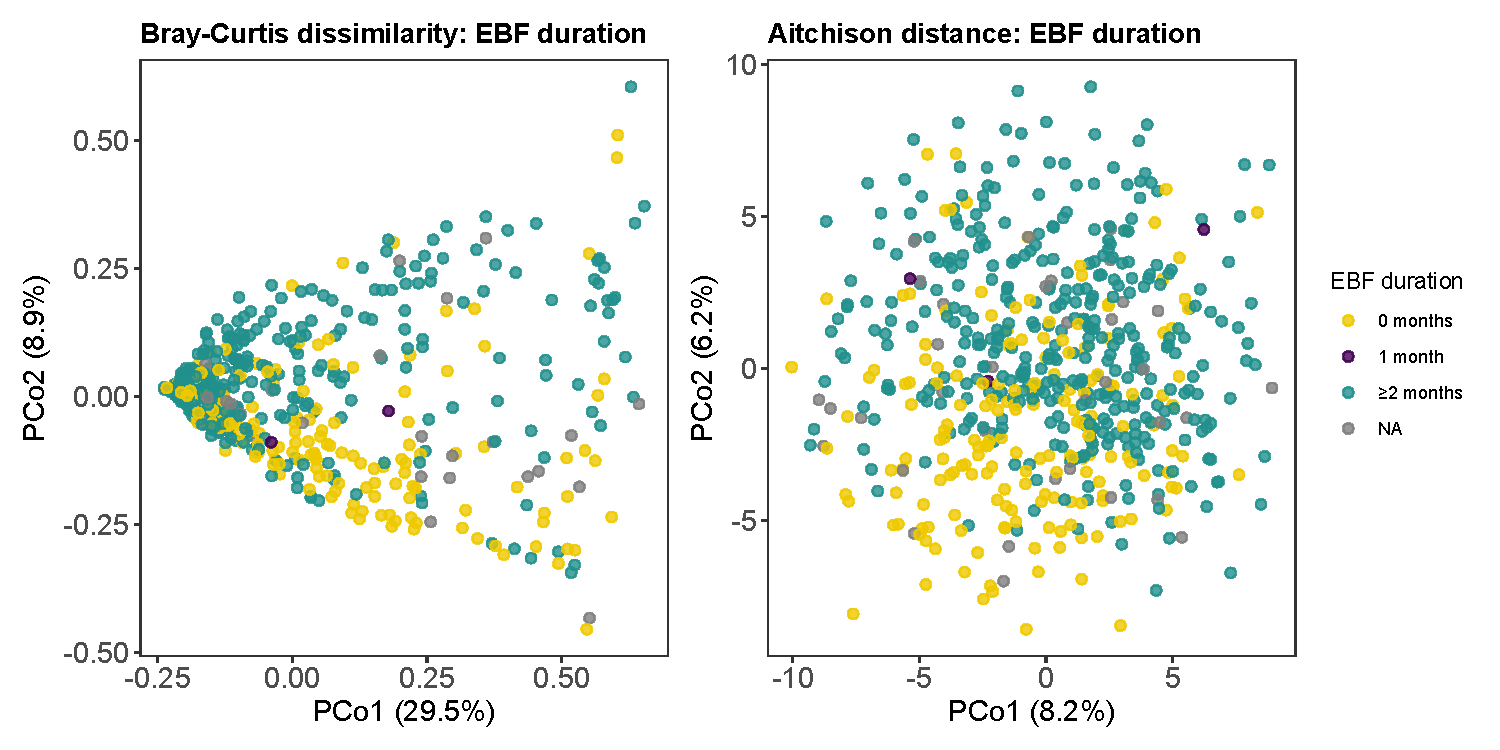
\includegraphics[width=\textwidth]{../ch07_application/figures/04_beta_diversity/thesis_PCoA_colored-5.pdf}
\caption{\textbf{Principal coordinate analysis by EBF duration.} Principal coordinate analysis of between-sample dissimilarities colored by EBF duration. The left panel shows Bray--Curtis dissimilarity computed from relative abundance profiles. The right panel shows Aitchison distance, computed as Euclidean distance after multiplicative replacement of zero counts followed by CLR transformation. Each point represents one stool sample, and the axis labels indicate the proportion of variation represented by the respective coordinate.}
\label{fig:7app:beta_diss:pcoa-exclusive-bf}
\end{figure}

%====================================
\subsection{PERMANOVA}
\label{sec:7app:beta:permanova}
%====================================

To formally assess whether cohort variables explain variation in the between-sample dissimilarity matrices, PERMANOVA was applied to both distance representations, following the distance-based testing framework described in Section~\ref{sec:3community:between:permanova}. The analysis was implemented using the \texttt{adonis2()} function from the \texttt{vegan} package \citep{oksanen2024vegan}. For each cohort variable and distance measure, a separate PERMANOVA model was fitted, and the observed pseudo-$F$ statistic was compared with a permutation distribution obtained from $999$ random permutations of the group labels. For EBF duration, the binary contrast defined in Section~\ref{sec:7app:default_data} was used. Samples with missing values for the respective cohort variable were excluded.

The resulting empirical $p$-values were subsequently refined using \texttt{permApprox}. The refinement used the default configuration described in Section~\ref{sec:6perm:workflow:default_config}, with three analysis-specific settings: a right-sided alternative was used because large pseudo-$F$ statistics indicate stronger evidence against the null hypothesis, the permutation distribution was centered around its median by setting \texttt{null\_center = ``median''}, and multiple testing adjustment was disabled. The reported values therefore correspond to nominal empirical and \texttt{permApprox}-refined $p$-values for each prespecified variable--distance combination. They are interpreted as variable-wise tests of association between each cohort variable and the respective dissimilarity matrix, rather than as a multiplicity-controlled family of simultaneous discoveries across all variables and distance measures.

Table~\ref{tab:7app:beta:permanova} summarizes the PERMANOVA results. For Bray--Curtis dissimilarity, all cohort variables except Sex show significant associations with community composition based on the refined $p$-values. The strongest evidence is observed for BF duration and EBF duration, followed by Country, Smoking, C-section, and Siblings. For Aitchison distance, all inspected cohort variables are significant at the $5\%$ level after $p$-value refinement, including Sex. The smallest refined $p$-values are again obtained for BF duration and EBF duration, indicating that breastfeeding-related variables explain the clearest variation in community composition among the variables considered.

\begin{table}[!htb]
\centering
\caption{\label{tab:7app:beta:permanova}\textbf{PERMANOVA results for between-sample dissimilarities.} PERMANOVA was applied separately to Bray--Curtis dissimilarity and Aitchison distance for all cohort variables. $n$ denotes the number of samples included in the respective test. Samples with missing values for the corresponding cohort variable were excluded, and for EBF duration the binary contrast defined in Section~\ref{sec:7app:default_data} was used. $F$ is the observed pseudo-$F$ statistic obtained with \texttt{adonis2}. \# exceed. denotes the number of permuted statistics greater than or equal to the observed statistic. $p$ (emp.) is the empirical permutation $p$-value based on $999$ permutations, and $p$ (GPD-refined) is the \texttt{permApprox}-refined $p$-value obtained from GPD tail approximation.}
\begin{threeparttable}
\begin{tabular}[t]{l@{\hspace*{1.5em}}rrr@{\hspace*{2em}}l@{\hspace*{2em}}l}
\toprule
Measure & $n$ & $F$ & \# exceed. & $p$ (emp.) & $p$ (GPD-refined)\\
\midrule
\addlinespace[0.3em]
\multicolumn{6}{l}{\textbf{Country}}\\
\hspace{1em}Bray--Curtis & 592 & 4.54 & 0 & 1.00e-03$^{**}$ & 1.18e-04$^{***}$\\
\hspace{1em}Aitchison & 592 & 2.58 & 0 & 1.00e-03$^{**}$ & 9.72e-14$^{***}$\\
\addlinespace[0.3em]
\multicolumn{6}{l}{\textbf{Sex}}\\
\hspace{1em}Bray--Curtis & 592 & 1.36 & 183 & 1.84e-01 & 1.84e-01\\
\hspace{1em}Aitchison & 592 & 1.45 & 33 & 3.40e-02$^{*}$ & 3.51e-02$^{*}$\\
\addlinespace[0.3em]
\multicolumn{6}{l}{\textbf{C-section}}\\
\hspace{1em}Bray--Curtis & 589 & 3.69 & 10 & 1.10e-02$^{*}$ & 7.56e-03$^{**}$\\
\hspace{1em}Aitchison & 589 & 2.48 & 0 & 1.00e-03$^{**}$ & 4.79e-07$^{***}$\\
\addlinespace[0.3em]
\multicolumn{6}{l}{\textbf{BF duration}}\\
\hspace{1em}Bray--Curtis & 580 & 14.30 & 0 & 1.00e-03$^{**}$ & 3.00e-11$^{***}$\\
\hspace{1em}Aitchison & 580 & 6.36 & 0 & 1.00e-03$^{**}$ & 3.91e-97$^{***}$\\
\addlinespace[0.3em]
\multicolumn{6}{l}{\textbf{EBF duration}}\\
\hspace{1em}Bray-Curtis & 554 & 19.58 & 0 & 1.00e-03$^{**}$ & 1.82e-08$^{***}$\\
\hspace{1em}Aitchison & 554 & 10.18 & 0 & 1.00e-03$^{**}$ & 1.18e-13$^{***}$\\
\addlinespace[0.3em]
\multicolumn{6}{l}{\textbf{Smoking}}\\
\hspace{1em}Bray--Curtis & 592 & 5.70 & 1 & 2.00e-03$^{**}$ & 6.81e-04$^{***}$\\
\hspace{1em}Aitchison & 592 & 3.09 & 0 & 1.00e-03$^{**}$ & 5.28e-10$^{***}$\\
\addlinespace[0.3em]
\multicolumn{6}{l}{\textbf{Siblings}}\\
\hspace{1em}Bray--Curtis & 503 & 2.23 & 20 & 2.10e-02$^{*}$ & 1.99e-02$^{*}$\\
\hspace{1em}Aitchison & 503 & 1.58 & 5 & 6.00e-03$^{**}$ & 1.80e-03$^{**}$\\
\bottomrule
\end{tabular}
\begin{tablenotes}
\item $^{***}:p<0.001$; $^{**}:p<0.01$; $^{*}:p<0.05$; $^{.}:p<0.1$.
\end{tablenotes}
\end{threeparttable}
\end{table}

The empirical permutation $p$-values illustrate the finite resolution of the permutation procedure. Whenever no permuted pseudo-$F$ statistic exceeds the observed value, the empirical $p$-value equals $1/(999+1)=0.001$. This occurs for several variables and for both distance measures. The \texttt{permApprox} refinement resolves this discreteness by modeling the upper tail of the corresponding permutation distribution. As a result, variables with the same empirical $p$-value can receive substantially different refined $p$-values, depending not only on the position of the observed statistic relative to the permutation distribution, but also on the shape and variability of that distribution.

This behavior is particularly visible for BF duration and EBF duration. For both variables, the observed pseudo-$F$ statistics are smaller for Aitchison distance than for Bray--Curtis dissimilarity, yet the \texttt{permApprox}-refined $p$-values are much smaller for Aitchison distance. This difference can be understood from the corresponding permutation distributions shown in Figure~\ref{fig:7app:beta_diss:permanova-permutation-distributions}. For the breastfeeding-related variables, the Aitchison permutation distributions are more concentrated, so that the observed statistics lie further in the extreme tail of their respective null distributions despite being numerically smaller than the Bray--Curtis pseudo-$F$ statistics. The refined $p$-values therefore reflect the extremeness of each observed statistic relative to its own distance-specific permutation distribution. The figure additionally includes C-section as a further early-life exposure related to birth mode. The corresponding permutation distributions for the remaining cohort variables are available in the \href{https://github.com/stefpeschel/phd_thesis/tree/main/ch07_application}{\texttt{ch07\_application}} folder of the thesis repository described at the beginning of this chapter.

\begin{figure}[!htb]
\centering
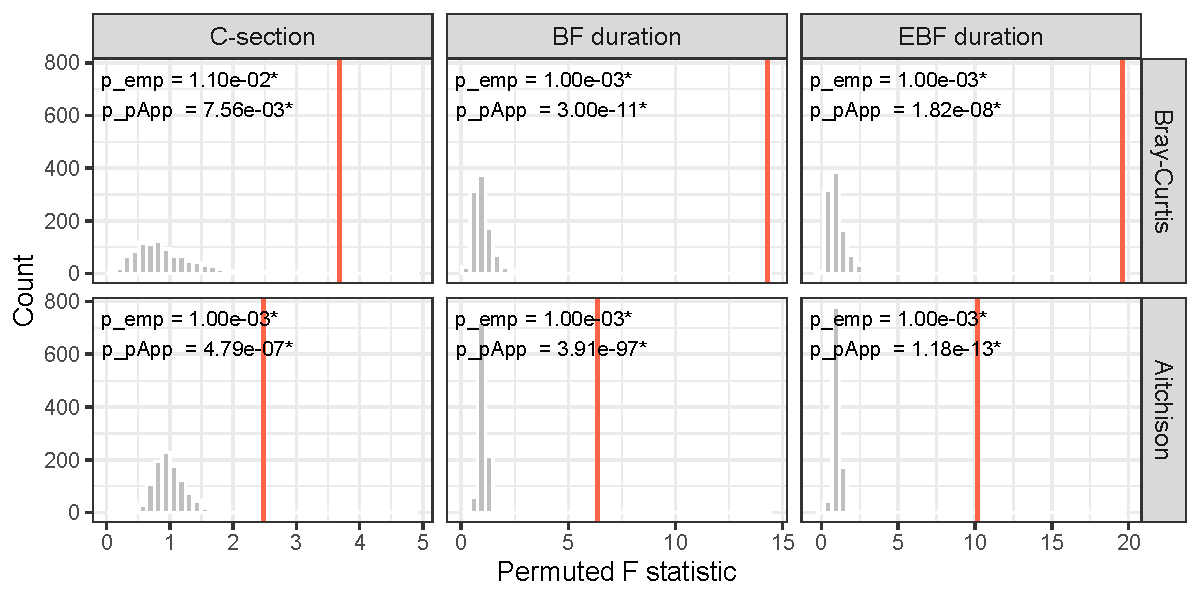
\includegraphics[width=\textwidth]{../ch07_application/figures/04_beta_diversity/thesis_permanova_permapprox_perm_dist_sel-1.pdf}
\caption{\textbf{PERMANOVA permutation distributions with $p$-value refinement.} Histograms show the permutation distributions of the PERMANOVA pseudo-$F$ statistic for each distance measure and three selected cohort variables: BF duration, EBF duration, and C-section. Red vertical lines indicate the observed pseudo-$F$ statistics. The displayed $p$-values correspond to the empirical permutation $p$-value and the \texttt{permApprox}-refined $p$-value. The breastfeeding-related variables illustrate that refined $p$-values depend on the position of the observed statistic relative to the full permutation distribution, and not only on the magnitude of the observed pseudo-$F$ statistic.}
\label{fig:7app:beta_diss:permanova-permutation-distributions}
\end{figure}

Taken together, the PERMANOVA results indicate that several cohort variables are associated with differences in overall community composition. The most consistent and strongest associations are observed for BF duration and EBF duration across both distance measures. Since PERMANOVA can also be sensitive to differences in within-group dispersion, the corresponding dispersion structure is examined in the following subsection using PERMDISP.

%====================================
\subsection{PERMDISP}
\label{sec:7app:beta:permdisp}
%====================================

PERMDISP was applied as described in Section~\ref{sec:3community:between:dispersion} to assess whether cohort variables were associated with differences in within-group dispersion. The same sample exclusions as in the PERMANOVA analysis were used. For EBF duration, this corresponds to the binary contrast defined in Section~\ref{sec:7app:default_data}. For each cohort variable and distance measure, distances of samples to their group centroid were computed and compared between groups. The analysis was implemented using the \texttt{betadisper()} and \texttt{permutest()} functions from the \texttt{vegan} package \citep{oksanen2024vegan}. Empirical $p$-values were computed using $999$ permutations and refined with \texttt{permApprox} using the same configuration as in the PERMANOVA analysis.

Table~\ref{tab:7app:beta:permdisp} summarizes the PERMDISP results. For Bray--Curtis dissimilarity, significant dispersion differences were observed for all variables except Sex. For Aitchison distance, dispersion differences were most pronounced for Country, BF duration, EBF duration, and Smoking, whereas C-section and Siblings showed weaker evidence and Sex showed no indication of dispersion differences. The strongest dispersion effects were again observed for the breastfeeding-related variables, particularly for Aitchison distance. These results indicate that the group differences detected by PERMANOVA should not be interpreted purely as shifts in multivariate location, because for several variables they are accompanied by differences in within-group dispersion.

\begin{table}[!htb]
\centering
\caption{\label{tab:7app:beta:permdisp}\textbf{PERMDISP results for between-sample dissimilarities.} PERMDISP was applied separately to Bray--Curtis dissimilarity and Aitchison distance for all cohort variables. $n$ denotes the number of samples included in the respective test. Samples with missing values for the corresponding cohort variable were excluded, and for EBF duration the binary contrast defined in Section~\ref{sec:7app:default_data} was used. $F$ is the observed test statistic for differences in distances to the group centroid. \# exceed. denotes the number of permuted statistics greater than or equal to the observed statistic. $p$ (emp.) is the empirical permutation $p$-value based on $999$ permutations, and $p$ (GPD-refined) is the \texttt{permApprox}-refined $p$-value obtained from GPD tail approximation.}
\begin{threeparttable}
\begin{tabular}[t]{l@{\hspace*{1.5em}}rrr@{\hspace*{2em}}l@{\hspace*{2em}}l}
\toprule
Measure & $n$ & $F$ & \# exceed. & $p$ (emp.) & $p$ (GPD-refined)\\
\midrule
\addlinespace[0.3em]
\multicolumn{6}{l}{\textbf{Country}}\\
\hspace{1em}Bray--Curtis & 592 & 10.60 & 4 & 5.00e-03$^{**}$ & 2.89e-03$^{**}$\\
\hspace{1em}Aitchison & 592 & 13.30 & 0 & 1.00e-03$^{**}$ & 2.22e-10$^{***}$\\
\addlinespace[0.3em]
\multicolumn{6}{l}{\textbf{Sex}}\\
\hspace{1em}Bray--Curtis & 592 & 2.67 & 215 & 2.16e-01 & 2.16e-01\\
\hspace{1em}Aitchison & 592 & 0.61 & 433 & 4.34e-01 & 4.34e-01\\
\addlinespace[0.3em]
\multicolumn{6}{l}{\textbf{C-section}}\\
\hspace{1em}Bray--Curtis & 589 & 8.87 & 34 & 3.50e-02$^{*}$ & 2.85e-02$^{*}$\\
\hspace{1em}Aitchison & 589 & 3.54 & 66 & 6.70e-02$^{.}$ & 6.93e-02$^{.}$\\
\addlinespace[0.3em]
\multicolumn{6}{l}{\textbf{BF duration}}\\
\hspace{1em}Bray--Curtis & 580 & 14.90 & 1 & 2.00e-03$^{**}$ & 5.88e-04$^{***}$\\
\hspace{1em}Aitchison & 580 & 32.10 & 0 & 1.00e-03$^{**}$ & 2.14e-26$^{***}$\\
\addlinespace[0.3em]
\multicolumn{6}{l}{\textbf{EBF duration}}\\
\hspace{1em}Bray-Curtis & 554 & 16.00 & 4 & 5.00e-03$^{**}$ & 4.21e-03$^{**}$\\
\hspace{1em}Aitchison & 554 & 61.04 & 0 & 1.00e-03$^{**}$ & 2.78e-14$^{***}$\\
\addlinespace[0.3em]
\multicolumn{6}{l}{\textbf{Smoking}}\\
\hspace{1em}Bray--Curtis & 592 & 6.74 & 47 & 4.80e-02$^{*}$ & 4.63e-02$^{*}$\\
\hspace{1em}Aitchison & 592 & 15.70 & 0 & 1.00e-03$^{**}$ & 2.63e-04$^{***}$\\
\addlinespace[0.3em]
\multicolumn{6}{l}{\textbf{Siblings}}\\
\hspace{1em}Bray--Curtis & 503 & 5.88 & 42 & 4.30e-02$^{*}$ & 4.77e-02$^{*}$\\
\hspace{1em}Aitchison & 503 & 2.63 & 83 & 8.40e-02$^{.}$ & 8.03e-02$^{.}$\\
\bottomrule
\end{tabular}
\begin{tablenotes}
\item $^{***}:p<0.001$; $^{**}:p<0.01$; $^{*}:p<0.05$; $^{.}:p<0.1$.
\end{tablenotes}
\end{threeparttable}
\end{table}


Figure~\ref{fig:7app:beta:centroid-distances} visualizes the PERMDISP results for the same three selected variables as above: BF duration, EBF duration, and C-section. The corresponding plots for the remaining cohort variables are available in the \href{https://github.com/stefpeschel/phd_thesis/tree/main/ch07_application}{\texttt{ch07\_application}} folder of the thesis repository described at the beginning of this chapter. For BF duration and EBF duration, the boxplots indicate clear differences in the heterogeneity of samples around their respective group centroids. This is especially visible for Aitchison distance, where groups with shorter or no breastfeeding tend to show larger distances to the centroid than the longer breastfeeding groups. C-section shows a weaker but still visible difference in dispersion, particularly for Bray--Curtis dissimilarity. These results indicate that the corresponding PERMANOVA findings should be interpreted as differences in overall group structure, while acknowledging that part of the signal may be attributable to differences in within-group dispersion rather than only to shifts in group centroids.

\begin{figure}[!htb]
\centering
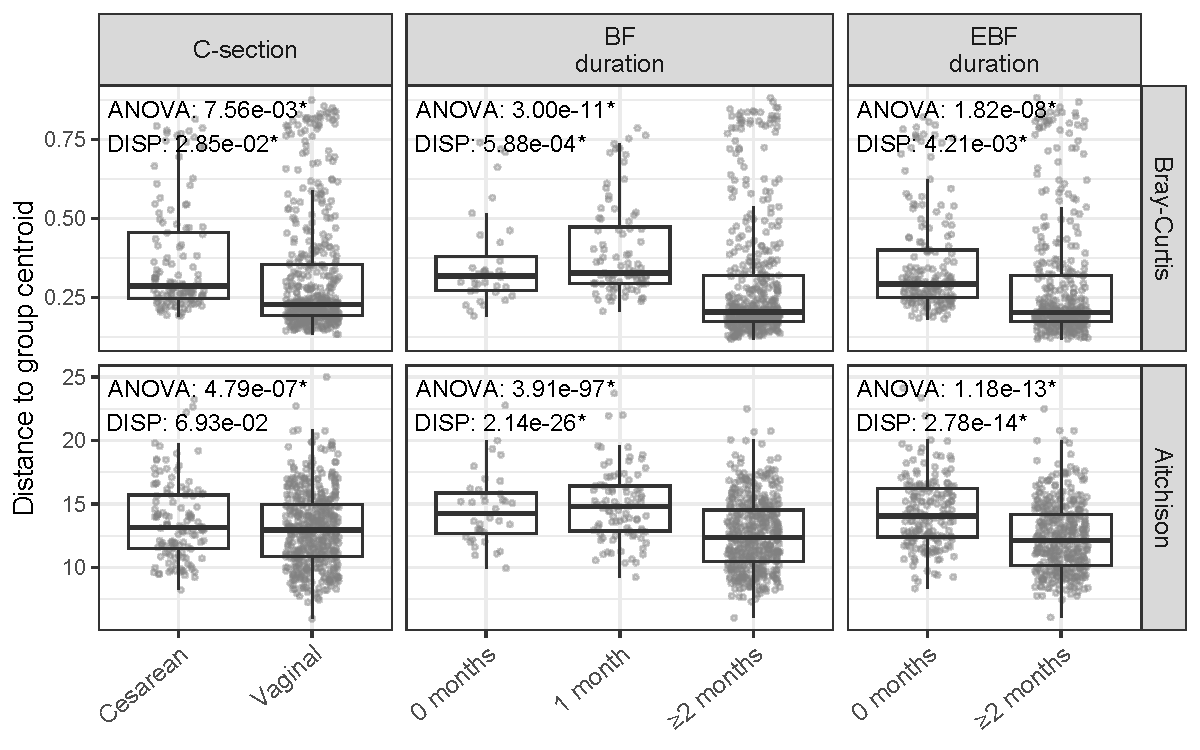
\includegraphics[width=\textwidth]{../ch07_application/figures/04_beta_diversity/thesis_beta_centroid_dist_sel-1.pdf}
\caption{\label{fig:7app:beta:centroid-distances}\textbf{Distances to group centroids for selected cohort variables.} Boxplots show the distances of samples to their respective group centroid for BF duration, EBF duration, and C-section. The upper row shows Bray--Curtis dissimilarity, and the lower row shows Aitchison distance. Points represent individual samples. The annotations report the \texttt{permApprox}-refined $p$-values from PERMANOVA and PERMDISP.}
\end{figure}

Overall, the PERMDISP analysis shows that dispersion differences are present for several cohort variables and are particularly pronounced for the breastfeeding-related variables. Thus, the corresponding PERMANOVA results should not be interpreted solely as evidence for shifts in group centroids. Instead, they indicate differences in the overall structure of the microbial community profiles, which may reflect both changes in average composition and differences in within-group heterogeneity. This observation is relevant for the subsequent analyses, because BF duration and EBF duration remain the variables with the most consistent community-level signal, but their effects appear to involve both location and dispersion components.

%%%%%%%%%%%%%%%%%%%%%%%%%%%%%%%%%%%%%
\section{Regression models for compositional responses}
\label{sec:7app:regression}
%%%%%%%%%%%%%%%%%%%%%%%%%%%%%%%%%%%%%

As a model-based complement to the distance-based analyses, CLR-based multivariate regression was applied to the genus-level microbiome profiles. The analysis followed the framework described in Section~\ref{sec:3community:regression} and used the default CLR representation defined in Section~\ref{sec:7app:default_data}. Whereas PERMANOVA assessed each cohort variable in a separate one-variable model, the regression approach allowed all covariates to be included jointly and each covariate to be tested conditionally on the others.

The regression model included the same cohort variables as the preceding community-level analyses, namely Country, Sex, C-section, BF duration, EBF duration, Smoking, and Siblings, as summarized in Table~\ref{tab:7app:sample_characteristics}. To ensure that all full-versus-reduced model comparisons were based on the same samples, a complete-case data set was constructed across all model covariates. In addition, the binary EBF contrast defined in Section~\ref{sec:7app:default_data} was used, so that the three samples with EBF duration of 1 month were excluded. The final regression analysis was therefore based on $n=484$ samples and $p=117$ genus-level taxa.

The fitted full model yields one coefficient for each model term and each CLR coordinate. Figure~\ref{fig:7app:regression:coefficient-heatmap} shows a reduced coefficient heatmap for the $20$ genera with the largest maximum absolute coefficient across all model terms. The heatmap is descriptive and is not used for taxon-level inference. It nevertheless provides a compact overview of the multivariate effect pattern and shows that the strongest fitted coefficients are not concentrated in a single covariate, but occur across several early-life variables. For categorical covariates, rows correspond to contrasts relative to the respective reference category. Positive coefficients indicate larger CLR values for the corresponding genus-level taxon relative to the sample-wise geometric mean, whereas negative coefficients indicate smaller CLR values on the same scale. The complete heatmap including all genus-level taxa is available in the \href{https://github.com/stefpeschel/phd_thesis/tree/main/ch07_application}{\texttt{ch07\_application}} folder of the thesis repository described at the beginning of this chapter.

\begin{figure}[!htb]
\centering
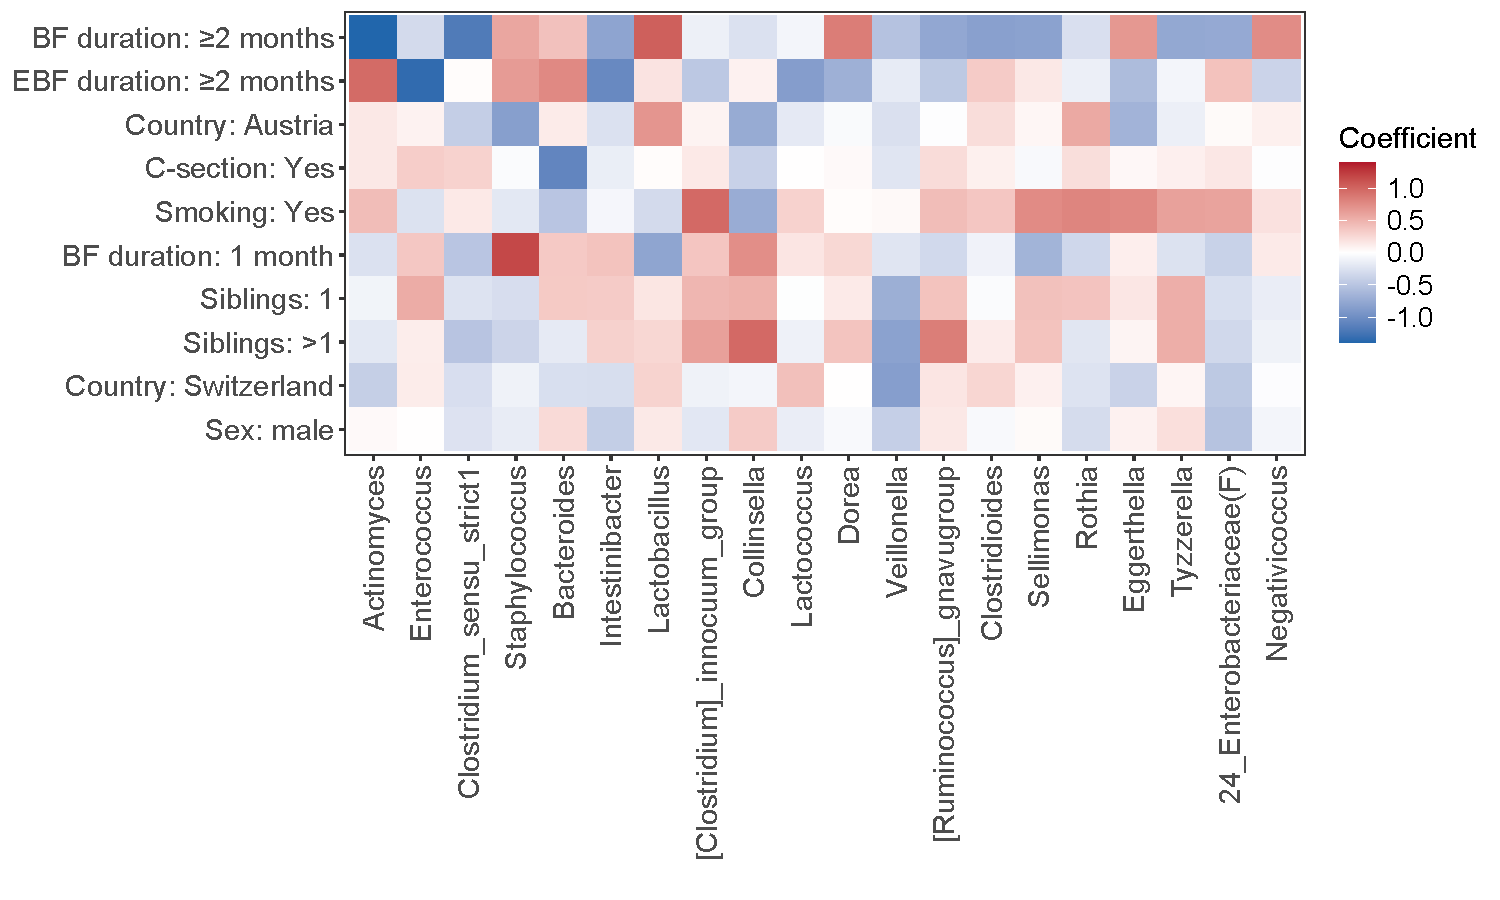
\includegraphics[width=\textwidth]{../ch07_application/figures/05_regression/thesis_coefficient_heatmap_top20-1.pdf}
\caption{\label{fig:7app:regression:coefficient-heatmap}\textbf{Reduced coefficient heatmap for CLR-based multivariate regression.} The heatmap shows fitted regression coefficients for the $20$ genus-level taxa with the largest maximum absolute coefficient across all model terms. Rows correspond to model terms, and columns correspond to genus-level taxa. For categorical covariates, coefficients represent contrasts relative to the reference category. Red values indicate positive coefficients on the CLR scale, whereas blue values indicate negative coefficients. The heatmap is descriptive and is not used for taxon-level inference.}
\end{figure}

For inference, each covariate was tested by comparing the full model with a reduced model in which the respective covariate was omitted, as described in Section~\ref{sec:3community:regression:testing}. The test statistic $t_j$ was defined as the reduction in multivariate residual sum of squares when covariate $j$ was included in the model. Larger values therefore indicate that the covariate explains more variation in the CLR-transformed microbial profile, conditional on the other covariates in the model. For each covariate, an empirical permutation $p$-value was computed from $999$ random permutations of the corresponding covariate. The resulting $p$-values were refined using \texttt{permApprox} with the same configuration as in the PERMANOVA analysis, namely a right-sided test, median centering of the permutation distribution, and no multiple testing adjustment. The reported $p$-values are therefore interpreted as nominal variable-wise $p$-values for the prespecified covariates.


The regression-based global tests in Table~\ref{tab:7app:regression:global-tests} identify EBF duration, Country, and BF duration as the strongest covariates, with no permuted statistic exceeding the observed statistic in $999$ permutations. The GPD refinement separates these three empirical $p$-values, which are all equal to $0.001$ before refinement. The smallest refined $p$-value is obtained for EBF duration, followed by Country and BF duration. Smoking also shows evidence of an association with the CLR-transformed microbial composition, whereas Siblings shows weaker evidence and Sex and C-section show no clear association after conditioning on the other covariates in the joint model.

\begin{table}[H]
\centering
\caption{\textbf{Permutation-based global tests in multivariate regression.} The table summarizes global covariate tests from the CLR-based multivariate regression model. All tests were performed on the same complete-case data set with $n=484$ samples and $117$ genus-level taxa. The statistic $t_j$ is the reduction in multivariate residual sum of squares when the covariate is added to the model. \# exceed. denotes the number of permuted statistics greater than or equal to the observed statistic. $p$ (emp.) is the empirical permutation $p$-value based on $999$ permutations, and $p$ (GPD-refined) is the \texttt{permApprox}-refined $p$-value obtained from GPD tail approximation.}
\label{tab:7app:regression:global-tests}
\centering
\begin{threeparttable}
\begin{tabular}[t]{lrrll}
\toprule
Variable & $t_j$ & \# exceed & $p$ (emp.) & $p$ (GPD-refined)\\
\midrule
Country & 699.03 & 0 & 1.00e-03$^{**}$ & 3.51e-06$^{***}$\\
Sex & 225.51 & 107 & 1.08e-01 & 1.08e-01\\
C-section & 217.65 & 147 & 1.48e-01 & 1.48e-01\\
BF duration & 641.49 & 0 & 1.00e-03$^{**}$ & 4.14e-05$^{***}$\\
EBF duration & 450.95 & 0 & 1.00e-03$^{**}$ & 8.78e-07$^{***}$\\
Smoking & 274.78 & 29 & 3.00e-02$^{*}$ & 2.41e-02$^{*}$\\
Siblings & 436.92 & 77 & 7.80e-02$^{.}$ & 7.22e-02$^{.}$\\
\bottomrule
\end{tabular}
\begin{tablenotes}
\item $^{***}:p<0.001$; $^{**}:p<0.01$; $^{*}:p<0.05$; $^{.}:p<0.1$.
\end{tablenotes}
\end{threeparttable}
\end{table}

These results partly agree with the distance-based PERMANOVA analysis, in which breastfeeding-related variables also showed the most consistent community-level associations. At the same time, the regression model has a different interpretation: each covariate is tested conditionally on the remaining covariates in the model, whereas the preceding PERMANOVA analyses considered separate one-variable models. The weaker regression signal for C-section therefore does not contradict the PERMANOVA result, but suggests that its contribution is less pronounced after accounting for the other early-life variables included in the multivariate model. Overall, the compositional-response regression supports the relevance of breastfeeding-related variables while providing a complementary model-based view of community-level covariate effects.

%%%%%%%%%%%%%%%%%%%%%%%%%%%%%%%%%%%%%
\section{Compositional equivalence}
\label{sec:7app:compositional-equivalence}
%%%%%%%%%%%%%%%%%%%%%%%%%%%%%%%%%%%%%

As a final community-level comparison, compositional equivalence was applied to selected two-group contrasts. In contrast to PERMANOVA, which operates on pairwise sample dissimilarities, compositional equivalence compares group mean composition in CLR space and summarizes the largest standardized coordinate-wise mean difference by a single global statistic, as described in Section~\ref{sec:3community:compositional_equivalence}. The analysis used the default CLR representation defined in Section~\ref{sec:7app:default_data}.

Because compositional equivalence is formulated as a two-group comparison, the analysis was restricted to selected binary or binarized contrasts. C-section, Sex, and Smoking were already binary variables. For BF duration and EBF duration, the main contrast compared samples with no breastfeeding to samples with breastfeeding duration $\ge 2$ months, omitting the sparse 1-month category as described in Section~\ref{sec:7app:default_data}. For Siblings, the variable was collapsed into children without siblings and children with at least one sibling. Country was omitted because this analysis focused on biologically interpretable two-group contrasts, whereas Country is a three-level cohort variable that may capture geographic, cohort-specific, and technical differences. The resulting contrast definitions are summarized in Table~\ref{tab:7app:comp-equivalence:contrasts}.

\begin{table}[H]
\centering
\caption{\textbf{Definition of selected two-group contrasts for compositional equivalence.} Group 1 and group 2 define the direction of the signed standardized CLR mean differences shown in Figure~\ref{fig:7app:comp-equivalence:top10-ebf}. Samples with missing values for the corresponding variable were excluded; for BF duration and EBF duration, the sparse 1-month category was additionally omitted.}
\label{tab:7app:comp-equivalence:contrasts}
\begin{tabular}[t]{llrlr}
\toprule
Contrast     & Group 1  & $n_1$ & Group 2 & $n_2$\\
\midrule
C-section    & Cesarean & 121 & Vaginal & 468\\
BF duration  & 0 months & 36 & $\ge 2$ months & 456\\
EBF duration & 0 months & 179 & $\ge 2$ months & 375\\
Sex          & Female   & 294 & Male & 298\\
Smoking      & No       & 529 & Yes & 63\\
Siblings     & 0        & 46 & $\ge 1$ & 457\\
\bottomrule
\end{tabular}
\end{table}

For each contrast, group differences were first evaluated coordinate-wise on the CLR scale. The resulting coordinate-wise contributions $m_i$, defined in Equation~\ref{eq:3community:comp_equivalence:coordinate_contribution}, form the building blocks of the global compositional equivalence statistic. They are therefore useful for describing which taxa contribute most to the maximum statistic, but are not interpreted as separate taxon-level hypothesis tests. Since $m_i$ is based on a squared mean difference, it does not contain information about the direction of the contrast. For visualization, the direction was therefore added through the signed standardized CLR mean difference $(\bar{y}_i^{(1)}-\bar{y}_i^{(2)})/\sqrt{\hat{\gamma}_{ii}}$, where positive values indicate larger CLR means in group 1 and negative values indicate larger CLR means in group 2. Since EBF duration was selected as the main grouping variable for subsequent comparative analyses, Figure~\ref{fig:7app:comp-equivalence:top10-ebf} shows the ten genera with the largest coordinate-wise contributions for this contrast. The corresponding plots for the remaining contrasts are available in the \href{https://github.com/stefpeschel/phd_thesis/tree/main/ch07_application}{\texttt{ch07\_application}} folder of the thesis repository described at the beginning of this chapter.

\begin{figure}[!htb]
\centering
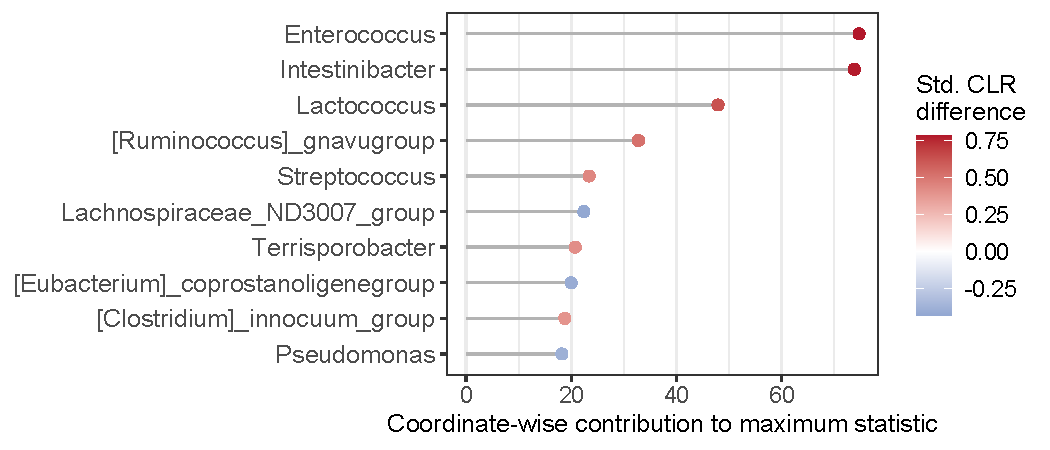
\includegraphics[width=0.85\textwidth]{../ch07_application/figures/06_comp_equivalence/thesis_taxon_contrast_top10_selected-1.pdf}
\caption{\label{fig:7app:comp-equivalence:top10-ebf}\textbf{Top coordinate-wise contributions for EBF duration.} The plot shows the ten genera with the largest coordinate-wise contributions $m_i$ from Equation~\ref{eq:3community:comp_equivalence:coordinate_contribution} for the contrast between no EBF and EBF duration $\ge 2$ months. Points show the squared, sample-size-weighted contribution to the maximum statistic. Colors indicate the signed standardized CLR mean difference and therefore encode the direction of the contrast. Positive values correspond to larger CLR means in group 1, as defined in Table~\ref{tab:7app:comp-equivalence:contrasts}.}
\end{figure}

For EBF duration, group 1 corresponds to children without EBF and group 2 to children with EBF duration $\ge 2$ months. Thus, positive signed standardized CLR mean differences indicate larger CLR values in the no-EBF group. The largest coordinate-wise contributions are observed for \emph{Enterococcus} and \emph{Intestinibacter}, followed by \emph{Lactococcus} and the \emph{[Ruminococcus] gnavus group}. Most of the largest signed differences are positive, indicating that the strongest coordinate-wise differences are driven by genera with higher relative representation, on the CLR scale, among children without EBF. Although the formal focus of the compositional equivalence test is the community-level maximum statistic, these taxon-wise contributions provide a useful descriptive link to the subsequent feature-level analyses.

The global compositional equivalence statistic $M_n$ was then computed as the maximum over all coordinate-wise contributions, as defined in Equation~\ref{eq:3community:comp_equivalence:maximum_statistic}. \citet{cao2018twosample} show that the centered statistic $M_n - 2\log(p) + \log\log(p)$ can be approximated by a Gumbel distribution under asymptotic assumptions, where $p$ denotes the number of CLR coordinates. These assumptions are not necessarily fulfilled in finite, sparse microbiome data. Indeed, \citet{sommer2022randomizationbased} compare this asymptotic approximation with permutation-based null distributions in their Supplementary Figure~J and show that the Gumbel approximation can differ markedly from the empirical permutation distribution, with corresponding differences in $p$-values. We performed the same comparison for the PASTURE contrasts in Appendix Figure~\ref{fig:app:7app:comp_equivalence_gumbel_comparison}. The corresponding asymptotic Gumbel $p$-values are included alongside the permutation-based $p$-values in Table~\ref{tab:7app:comp-equivalence:pvals}. As in \citep{sommer2022randomizationbased}, the permutation distributions were not uniformly well approximated by the Gumbel distribution, and the asymptotic $p$-values differed from the permutation-based $p$-values for several contrasts.

Therefore, the following inference follows the randomization-based approach of \citet{sommer2022randomizationbased} rather than relying on the asymptotic Gumbel approximation. For each contrast, the observed value of $M_n$ was compared with a permutation distribution obtained from $999$ random permutations of the group labels. Since large values of $M_n$ indicate stronger evidence against equality of mean CLR composition, a right-sided test was used. The resulting empirical $p$-values were refined with \texttt{permApprox} using the same configuration as in the preceding community-level analyses, including median centering of the permutation distribution and no multiple testing adjustment. The reported $p$-values are therefore interpreted as nominal $p$-values for the selected two-group contrasts.

The results in Table~\ref{tab:7app:comp-equivalence:pvals} indicate clear differences in mean CLR composition for C-section, BF duration, and EBF duration. The strongest signal is observed for EBF duration, for which the observed statistic is substantially larger than for the other contrasts and exceeds all permuted statistics. This extremeness cannot be expressed by the empirical permutation $p$-value, which is limited by the number of permutations, but is reflected in the much smaller GPD-refined $p$-value. BF duration and C-section also show significant differences, although their refined $p$-values are considerably less extreme. In contrast, Sex, Smoking, and Siblings show no evidence against equality of mean CLR composition for the selected two-group contrasts.

\begin{table}[H]
\centering
\caption{\textbf{Compositional equivalence results for selected contrasts.} The group definitions and corresponding sample sizes are given in Table~\ref{tab:7app:comp-equivalence:contrasts}. $M_n$ is the maximum standardized squared CLR mean difference. $M_n^c = M_n - 2\log(p) + \log\log(p)$ is the centered statistic used for the asymptotic Gumbel approximation. \# exceed: number of permuted statistics $\geq$ observed. $p$ (emp.): empirical permutation $p$-value ($999$ permutations); $p$ (GPD-ref.): $p$-value refined with \texttt{permApprox}; $p$ (asym.): asymptotic Gumbel $p$-value.}
\label{tab:7app:comp-equivalence:pvals}
\centering
\begin{threeparttable}
\begin{tabular}[t]{lrrrlll}
\toprule
Contrast & $M_n$ & $M_n^c$ & \# exceed & $p$ (emp.) & $p$ (GPD-ref.) & $p$ (asym.)\\
\midrule
C-section & 25.06 & 17.09 & 0 & 1.00e-03$^{**}$ & 5.26e-04$^{***}$ & 1.09e-04$^{***}$\\
BF duration & 33.16 & 25.19 & 3 & 4.00e-03$^{**}$ & 2.99e-03$^{**}$ & 1.91e-06$^{***}$\\
EBF duration & 74.72 & 66.75 & 0 & 1.00e-03$^{**}$ & 2.31e-66$^{***}$ & 1.78e-15$^{***}$\\
Sex & 9.79 & 1.83 & 157 & 1.58e-01 & 1.58e-01 & 2.03e-01\\
Smoking & 13.91 & 5.95 & 119 & 1.20e-01 & 1.20e-01 & 2.84e-02$^{*}$\\
\addlinespace
Siblings & 14.17 & 6.21 & 123 & 1.24e-01 & 1.24e-01 & 2.50e-02$^{*}$\\
\bottomrule
\end{tabular}
\begin{tablenotes}
\item $^{***}:p<0.001$; $^{**}:p<0.01$; $^{*}:p<0.05$; $^{.}:p<0.1$.
\end{tablenotes}
\end{threeparttable}
\end{table}

Overall, compositional equivalence supports the central role of breastfeeding-related variables in the PASTURE application. In particular, EBF duration shows a strong difference in mean CLR composition between children without EBF and children with EBF duration $\ge 2$ months. Together with the PERMANOVA, PERMDISP, and regression results, this motivates using EBF duration as the main grouping variable for the subsequent feature-level and network-based analyses.

%%%%%%%%%%%%%%%%%%%%%%%%%%%%%%%%%%%%%
\section{Exploratory feature-level analysis}
\label{sec:7app:feature-level-exploration}
%%%%%%%%%%%%%%%%%%%%%%%%%%%%%%%%%%%%%

The preceding community-level analyses identified the breastfeeding-related variables as the most consistent variables associated with differences in the infant gut microbiome. Both BF duration and EBF duration showed strong signals across the community-level analyses. In the PERMANOVA and PERMDISP analyses presented in Section~\ref{sec:7app:beta}, the effects were larger for BF duration, whereas EBF duration yielded smaller $p$-values in the regression and compositional equivalence analyses presented in Sections~\ref{sec:7app:regression} and~\ref{sec:7app:compositional-equivalence}. Since a binary grouping based on BF duration would result in more unbalanced group sizes, EBF duration was selected as the main grouping variable for the subsequent feature-level and network-based analyses. The following comparative analyses therefore use the binary EBF contrast defined in Section~\ref{sec:7app:default_data}, comparing children without EBF ($n=179$) with children with EBF duration $\ge 2$ months ($n=375$).

As a first step, exploratory taxon-level summaries were used to characterize the genus-level composition of the default analysis data set and the two EBF groups. Relative abundances were used for descriptive composition summaries, whereas CLR coordinates were used for visualizing transformed taxon profiles. Both representations are defined in Section~\ref{sec:7app:default_data}. The exploratory analyses are descriptive and are not intended to provide formal taxon-level inference.

Figure~\ref{fig:7app:exploration:prevalence-abundance} first gives an overview of the retained genera without considering the EBF grouping. It displays each genus by its prevalence and mean relative abundance in the filtered genus-level data set. Most retained genera have low mean relative abundance and moderate prevalence, whereas a smaller set of dominant genera is both highly prevalent and comparatively abundant. \emph{Bifidobacterium} is located in the upper right region, indicating high prevalence and high mean relative abundance. Other dominant genera, including \emph{Escherichia-Shigella}, \emph{Streptococcus}, \emph{Bacteroides}, \emph{Enterococcus}, and the \emph{[Ruminococcus] gnavus group}, also stand out from the remaining low-abundance genera. This plot provides the feature-level background for the subsequent group-specific summaries.

\begin{figure}[!htb]
\centering
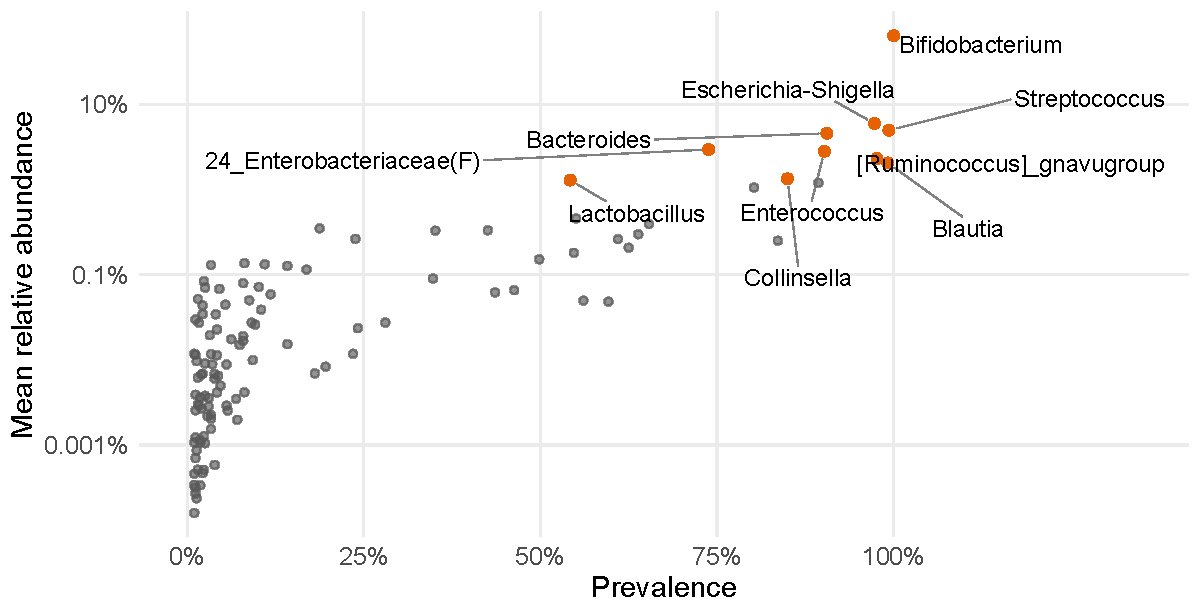
\includegraphics[width=\textwidth]{../ch07_application/figures/07_exploration/thesis_prevalence_abundance-1.pdf}
\caption{\label{fig:7app:exploration:prevalence-abundance}\textbf{Prevalence and mean relative abundance of retained genera.} Each point represents one genus after prevalence filtering. The highlighted and labeled points show the ten genera with the largest mean relative abundances. The y-axis is displayed on a logarithmic scale to show both dominant and low-abundance genera.}
\end{figure}

The following plots focus on the comparison between the two EBF groups. Figure~\ref{fig:7app:exploration:composition-barplot} shows the mean relative abundance of the dominant genera by EBF group. The composition is dominated by \emph{Bifidobacterium} in both groups, reflecting the characteristic dominance of this genus in the early infant gut. The remaining genera contribute smaller proportions, with visible differences between the non-EBF and EBF groups for several taxa, including \emph{Bacteroides}, \emph{Enterococcus}, \emph{Streptococcus}, and \emph{Escherichia-Shigella}. Since this plot is based on relative abundances, the displayed patterns may be affected by compositional effects and should not be interpreted as absolute abundance changes. The CLR coordinates shown in Figure~\ref{fig:7app:exploration:clr-violin} provide a complementary log-ratio view of the same group comparison. The group labeled ``not compared'' is shown for completeness and contains samples not used in the binary EBF comparison.

\begin{figure}[!htb]
\centering
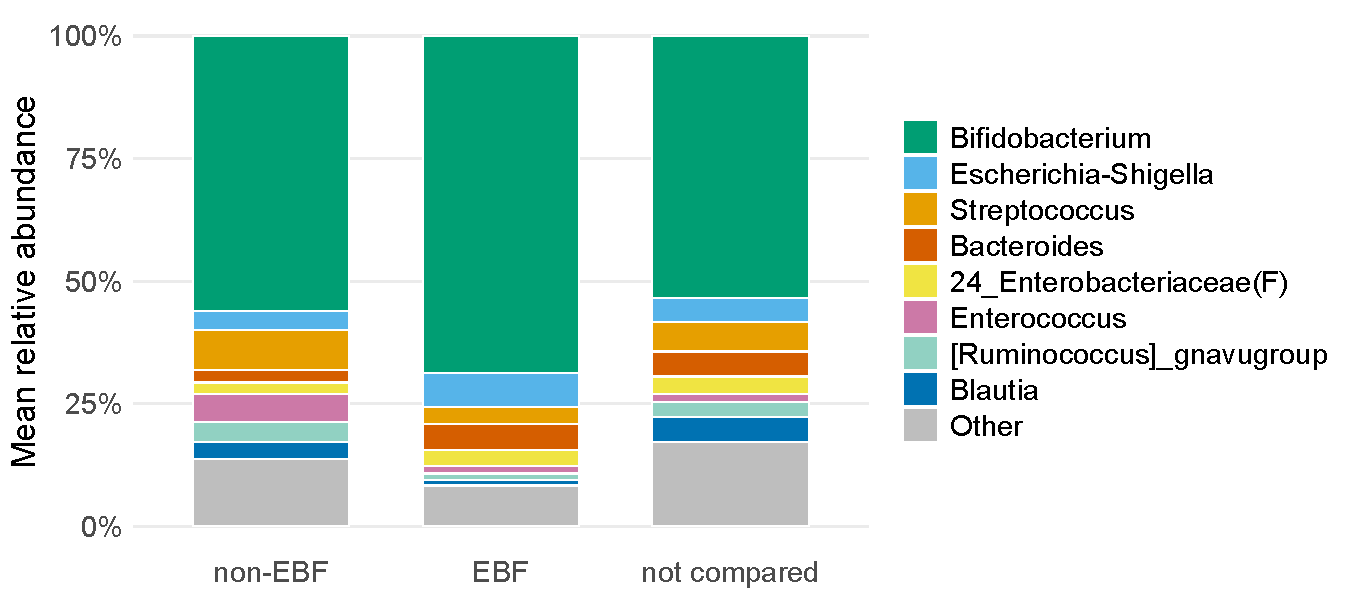
\includegraphics[width=\textwidth]{../ch07_application/figures/07_exploration/thesis_relative_abundance_barplot-1.pdf}
\caption{\label{fig:7app:exploration:composition-barplot}\textbf{Mean genus-level composition by EBF group.} Stacked bars show the mean relative abundances of the dominant genera in the non-EBF group, the EBF group, and samples not included in the EBF comparison. The category ``Other'' summarizes all remaining genera. The plot is descriptive and is based on relative abundances.}
\end{figure}

Figure~\ref{fig:7app:exploration:clr-violin} shows the distributions of CLR coordinates for six dominant genera in the two EBF groups. This representation is closer to the transformed scale used in the following feature-level analyses and avoids interpreting relative-abundance differences as absolute abundance changes. The violin plots indicate differences not only in location but also in distributional shape and variability between the two EBF groups. For example, \emph{Enterococcus} shows higher CLR coordinates in the non-EBF group, whereas \emph{Bacteroides} tends to show higher CLR coordinates in the EBF group. These patterns suggest that feature-level comparisons should not be restricted to mean differences alone. Instead, differential abundance and differential distribution analyses may provide complementary information.

\begin{figure}[!htb]
\centering
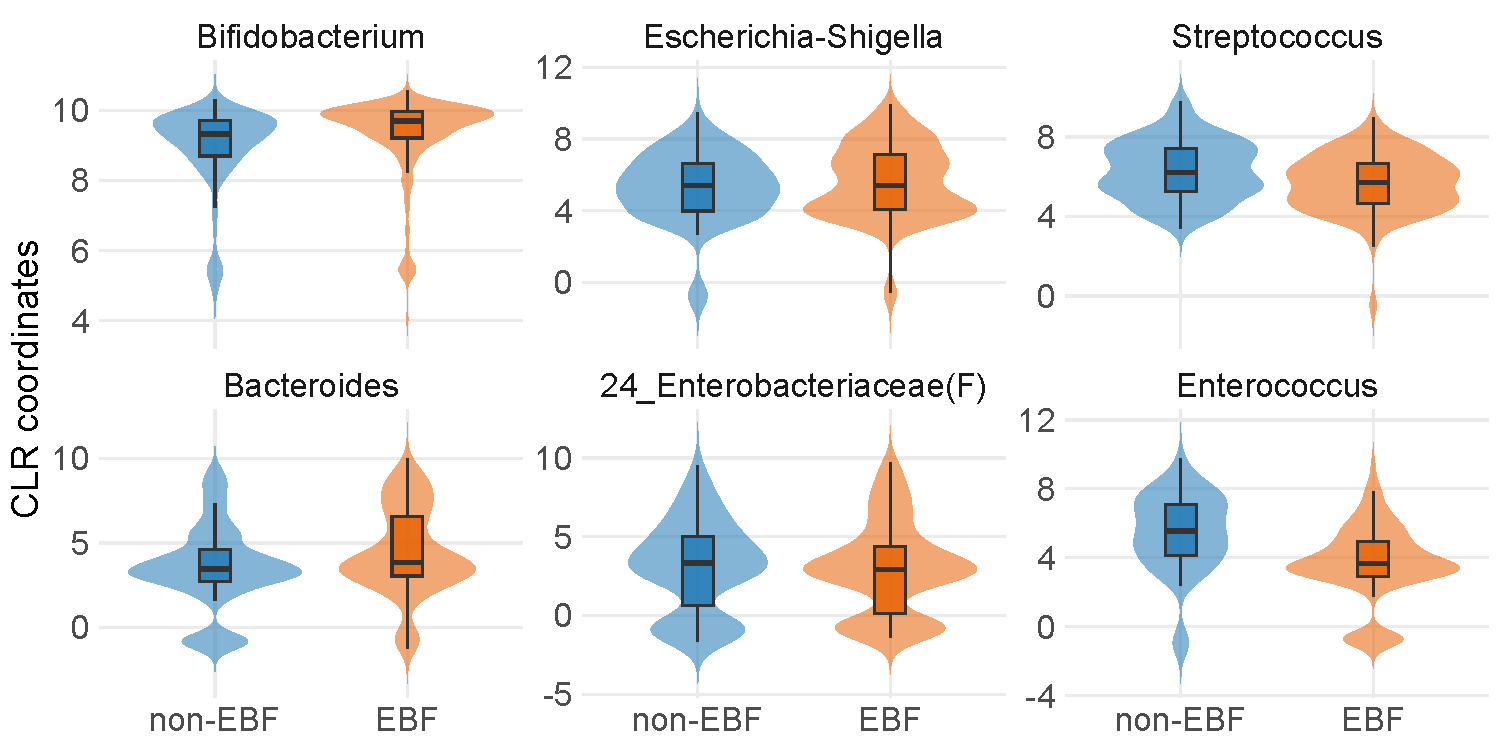
\includegraphics[width=\textwidth]{../ch07_application/figures/07_exploration/thesis_selected_taxon_violin-1.pdf}
\caption{\textbf{CLR coordinates of selected dominant genera by EBF group.} Violin plots and embedded boxplots show the distributions of CLR coordinates for six dominant genera in the non-EBF and EBF groups. Zeros were handled by multiplicative replacement before CLR transformation. The plot is descriptive and does not represent feature-level hypothesis tests.}
\label{fig:7app:exploration:clr-violin}
\end{figure}

Taken together, the exploratory feature-level summaries show visible group differences in the relative-abundance composition and CLR-coordinate distributions of several dominant genera. These observations are consistent with the community-level results but remain descriptive. Formal feature-level comparisons are therefore performed in the following sections using differential abundance and differential distribution analyses.

%%%%%%%%%%%%%%%%%%%%%%%%%%%%%%%%%%%%%
\section{Differential abundance analysis}
\label{sec:7app:differential-abundance}
%%%%%%%%%%%%%%%%%%%%%%%%%%%%%%%%%%%%%

The exploratory feature-level summaries in the previous section suggested visible differences between the two EBF groups for several dominant genera. To formally assess feature-wise abundance differences, differential abundance analysis was performed using DACOMP, as introduced in Section~\ref{sec:4feature:dacomp}. The method is implemented in the R package \texttt{dacomp} \citep{Brill2021dacomp}. The analysis used the binary EBF contrast defined in Section~\ref{sec:7app:default_data}, comparing children without EBF ($n=179$) with children with EBF duration $\ge 2$ months ($n=375$).

%====================================
\subsection{Analysis setup and DACOMP reference set}
\label{sec:7app:differential-abundance:setup}
%====================================

DACOMP was applied to the genus-level count matrix corresponding to the default analysis data set defined in Section~\ref{sec:7app:default_data}, yielding $n=554$ samples and $117$ retained genera. This is a method-specific deviation from the CLR-based representation used in the preceding community-level analyses. DACOMP uses a count-based reference framework: compositionality is addressed by comparing each tested taxon relative to a set of taxa selected to be comparatively stable across samples, while differences in library size are handled through a method-specific subsampling step within the testing procedure. The resulting differential abundance statements are therefore relative to the corresponding reference structure and should not be interpreted as statements about absolute microbial abundances. We used \texttt{dacomp}'s ability to test all retained taxa, including taxa selected for the reference set. When such a reference taxon was itself tested, it was temporarily removed from the reference set for that test.

The reference selection step is summarized in Figure~\ref{fig:7app:da:reference-score}. The diagnostic plot shows the DACOMP reference score against the prevalence of each retained genus. Genera selected as reference taxa are shown in green, while the remaining genera are shown in grey. In total, $91$ of the $117$ retained genera were selected as reference taxa using a minimum total reference abundance criterion of $50$. Most reference taxa have low to moderate prevalence and low DACOMP scores, indicating comparatively stable behavior according to the reference-selection criterion. A few highly prevalent genera, including \emph{Bifidobacterium}, \emph{Blautia}, and \emph{Akkermansia}, were also selected as reference taxa.

\begin{figure}[!htb]
\centering
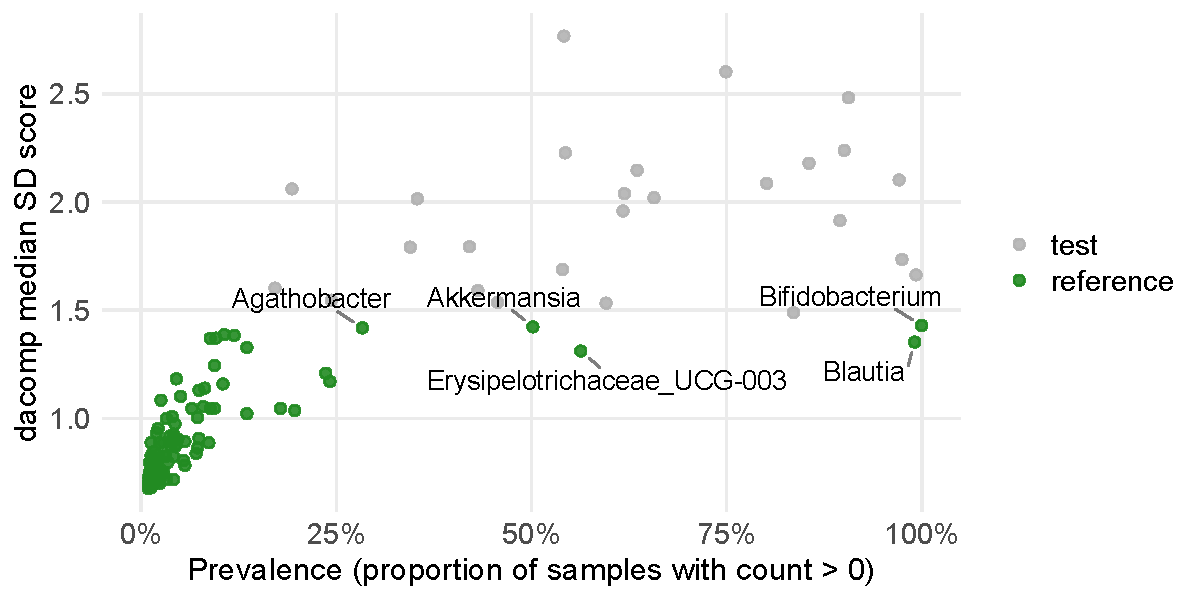
\includegraphics[width=0.9\textwidth]{../ch07_application/figures/08_diff_abundance/thesis_dacomp_reference_score_plot-1.pdf}
\caption{\label{fig:7app:da:reference-score}\textbf{DACOMP reference-score diagnostic.} Each point represents one retained genus. The x-axis shows the prevalence, defined as the proportion of samples with a positive count, and the y-axis shows the DACOMP median standard-deviation score used for reference selection. Green points indicate genera selected for the reference set, and grey points indicate genera not selected as reference taxa. Labeled genera are selected reference taxa with prevalence of at least $25\%$.}
\end{figure}

%====================================
\subsection{Permutation resolution and p-value refinement}
\label{sec:7app:differential-abundance:pvalue-refinement}
%====================================

\begin{figure}[H]
	\centering
	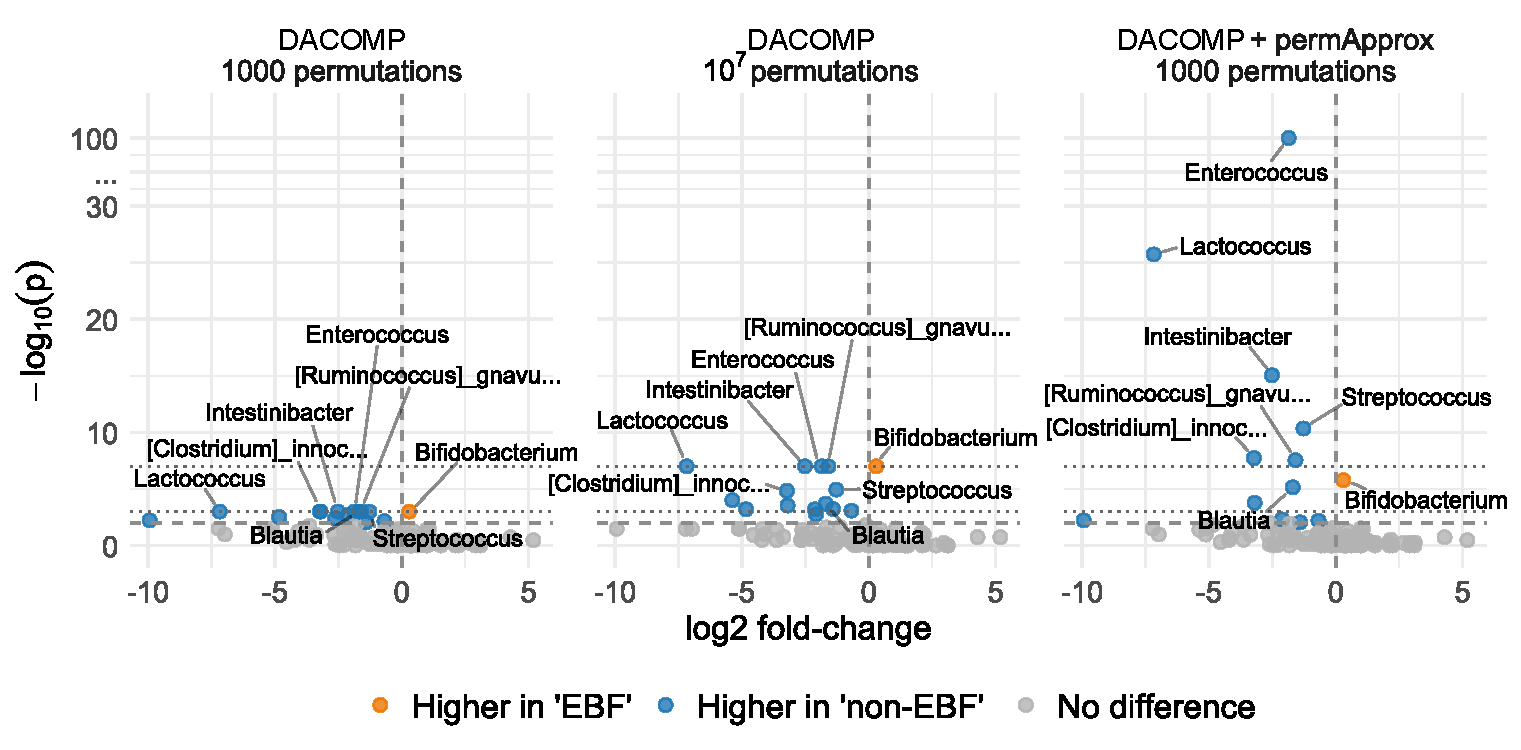
\includegraphics[width=\textwidth]{../ch07_application/figures/08_diff_abundance/thesis_volcano_plot_raw-2.pdf}
	\caption{\label{fig:7app:da:volcano}\textbf{Differential abundance analysis with DACOMP and \texttt{permApprox}.} Volcano plots show log$_2$ fold-changes of mean relative abundance, computed as EBF versus non-EBF, against raw differential abundance $p$-values. The left panel shows empirical DACOMP $p$-values obtained with $1000$ permutations, the middle panel shows empirical DACOMP $p$-values obtained with $10^7$ permutations, and the right panel shows constrained \texttt{permApprox}-refined $p$-values obtained from the $1000$-permutation DACOMP run. Orange points indicate genera with higher mean relative abundance in the EBF group, and blue points indicate genera with higher mean relative abundance in the non-EBF group. Grey points have raw $p$-values above $\alpha=0.01$. The horizontal dashed line marks $\alpha=0.01$ for visual reference. The two dotted horizontal lines indicate the smallest empirical $p$-values attainable with $1000$ and $10^7$ permutations, respectively.}
\end{figure}

After reference selection, DACOMP was run with different permutation budgets to evaluate the effect of finite permutation resolution. The main comparison considered DACOMP with $1000$ permutations, DACOMP with $10^7$ permutations, and DACOMP with $1000$ permutations followed by constrained \texttt{permApprox} refinement. Since the DACOMP statistic is non-negative and larger values indicate stronger evidence against the null hypothesis, $p$-value approximation was performed as a right-tailed problem. The constrained \texttt{permApprox} workflow was applied to the observed and permuted DACOMP statistics using the support-constrained GPD tail approximation described in Chapter~\ref{ch:permapprox}. We used the default configuration described in Section~\ref{sec:6perm:workflow:default_config}, which also corresponds to the default settings of the R implementation. Thus, the empirical $p$-values from the $1000$-permutation DACOMP run were retained in the bulk, whereas small tail $p$-values were refined by constrained GPD approximation.

Figure~\ref{fig:7app:da:volcano} compares the raw $p$-values obtained from the three differential abundance analyses. Raw $p$-values are shown in this plot to display the effect of permutation \text{resolution} and tail approximation without conflating it with multiplicity correction. The corresponding adjusted $p$-values are reported in Appendix Table~\ref{tab:app:7app:diff_abundance_adj_pvalues}. With $1000$ permutations, several taxa reach the empirical lower bound of the permutation $p$-values, so that the strongest effects cannot be distinguished on the $p$-value scale. Increasing the permutation budget to $10^7$ resolves the empirical tail more finely and separates the strongest signals. In this run, \emph{Lactococcus}, \emph{Intestinibacter}, \emph{Enterococcus}, the \emph{[Ruminococcus] gnavus group}, and \emph{Bifidobacterium} appear among the taxa with the smallest raw $p$-values, followed by the \emph{[Clostridium] innocuum group}, \emph{Streptococcus}, and \emph{Blautia}. The constrained \texttt{permApprox} refinement based on only $1000$ permutations identifies largely the same set of taxa as strongest tail signals, but the exact ordering and magnitude of the refined $p$-values differ for some taxa.

\begin{figure}[H]
	\centering
	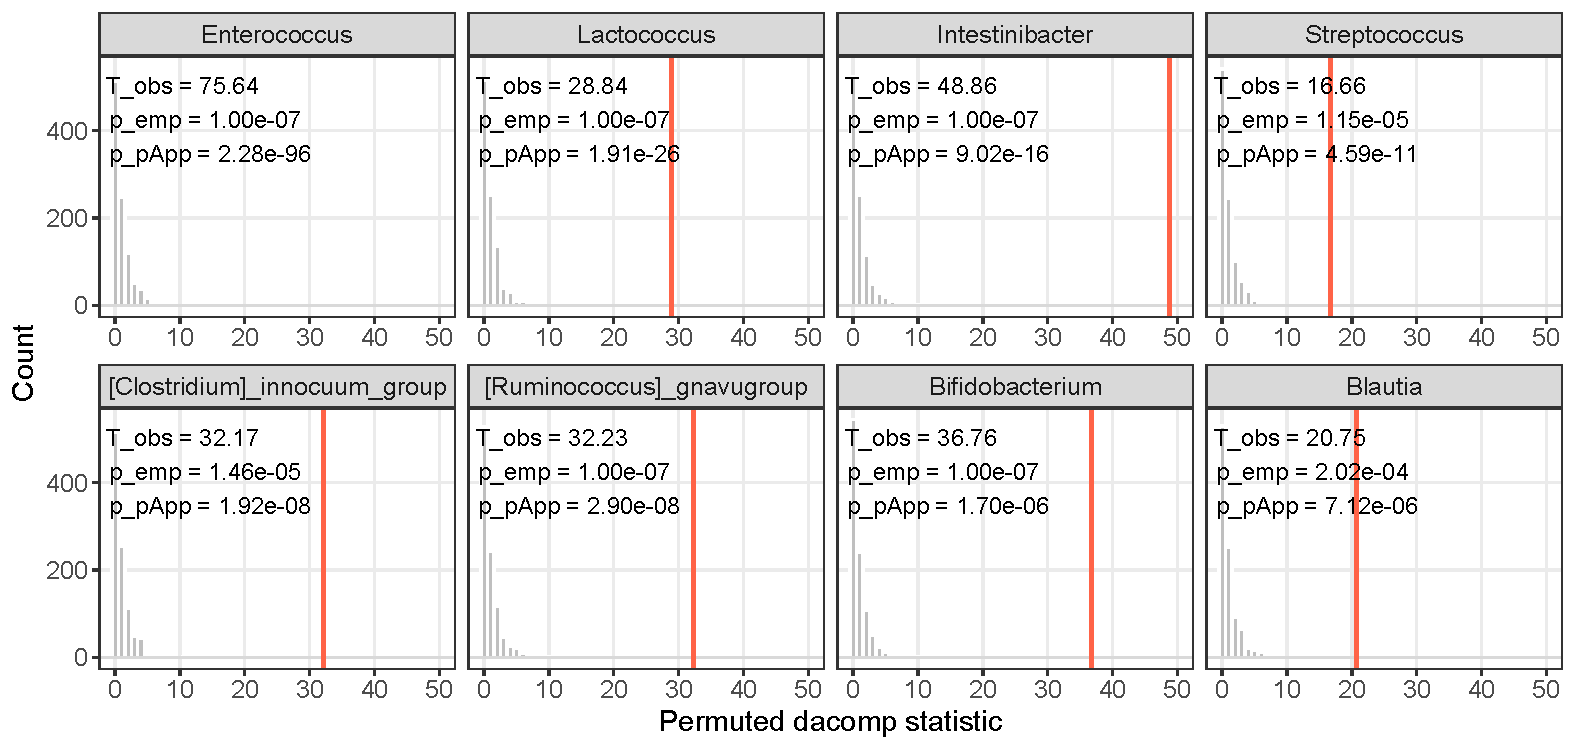
\includegraphics[width=\textwidth]{../ch07_application/figures/08_diff_abundance/thesis_permutation_distribution_plot-1.pdf}
	\caption{\label{fig:7app:da:perm-dist}\textbf{Permutation distributions for selected genera.} Histograms show the permutation distributions of the DACOMP test statistic for the eight genera labeled in Figure~\ref{fig:7app:da:volcano}. Red vertical lines indicate the observed test statistics. The empirical $p$-values shown in the panels are based on the $10^7$-permutation DACOMP run, while the \texttt{permApprox} $p$-values are obtained from the constrained GPD refinement of the $1000$-permutation run. The x-axis is restricted to the interval from $0$ to $50$ for better readability. Observed test statistics outside this range are therefore not visible as vertical lines.}
\end{figure}


The permutation distributions in Figure~\ref{fig:7app:da:perm-dist} illustrate why the $p$-value ranking is not determined by the observed test statistic alone. The panels show the empirical permutation distributions for the eight labeled taxa, together with the observed DACOMP statistic. For \emph{[Clostridium] innocuum group} and the \emph{[Ruminococcus] gnavus group}, the observed DACOMP statistics are almost identical and the permutation distributions have a similar shape, which makes the similar \texttt{permApprox}-refined $p$-values plausible. In contrast, differences between taxa such as \emph{Streptococcus} and \emph{Bifidobacterium} reflect more subtle aspects of the permutation distribution, including the spread of the null distribution, the frequency of large permuted statistics, and the location of the observed statistic relative to the fitted tail. Thus, the refined $p$-value is not a monotone transformation of the observed statistic alone, but combines information from the observed statistic and the estimated tail behavior of the permutation distribution.


The comparison between the empirical $10^7$-permutation $p$-values and the \texttt{permApprox}-refined $p$-values should not be interpreted as an expectation of exact numerical agreement. Both approaches depend on the sampled permutation statistics, and their tail behavior can vary with the random seed. The purpose of the comparison is instead to assess whether the tail approximation translates the observed statistic and the \text{available} permutation distribution into a meaningful refined $p$-value at a much lower computational cost. In this application, the constrained \texttt{permApprox} analysis removes the empirical lower bound of the $1000$-permutation run, separates strong tail signals that are indistinguishable under the smaller permutation budget, and yields results that are broadly coherent with the much more expensive $10^7$-permutation analysis.

%====================================
\subsection{Runtime comparison}
\label{sec:7app:differential-abundance:runtime}
%====================================

The runtime comparison in Table~\ref{tab:7app:da:runtime} illustrates the computational motivation for this refinement. DACOMP with $1000$ permutations required only $1.69$ seconds, but its smallest attainable empirical $p$-value is limited by the coarse permutation grid. Increasing the number of permutations to $10^6$ already required $1675.86$ seconds, corresponding to approximately $27.93$ minutes, while the $10^7$-permutation run required $20963.69$ seconds, corresponding to approximately $5.82$ hours. In contrast, the combined runtime of DACOMP with $1000$ permutations and constrained \texttt{permApprox} refinement was $8.89$ seconds. Thus, compared with the $1000$-permutation DACOMP run alone, the constrained \texttt{permApprox} refinement added only a small absolute runtime overhead, while providing continuous tail $p$-values below the empirical lower bound of the $1000$-permutation analysis.

\begin{table}[!htb]
\centering
\caption{\label{tab:7app:da:runtime}\textbf{Runtime comparison for DACOMP and $p$-value refinement.} Runtime was measured for DACOMP with different permutation budgets and for the combined workflow consisting of DACOMP with $1000$ permutations followed by constrained \texttt{permApprox} refinement. Computations were run on a Linux-based compute node equipped with an Intel Xeon E7-4850 v4 CPU (2.10 GHz) and 170 GB RAM.}
\begin{tabular}{lrrr}
\toprule
Method & Permutations & Runtime (seconds) & Runtime \\
\midrule
DACOMP & $1000$ & $1.69$ & $0.03$ min \\
DACOMP & $10^6$ & $1675.86$ & $27.93$ min \\
DACOMP & $10^7$ & $20963.69$ & $5.82$ h~~~\, \\
DACOMP + \texttt{permApprox} & $1000$ & $8.89$ & $0.15$ min \\
\bottomrule
\end{tabular}
\end{table}

%====================================
\subsection{Descriptive characterization of selected genera}
\label{sec:7app:differential-abundance:selected-genera}
%====================================

The preceding analyses identified eight genera with particularly small differential abundance $p$-values. To relate these formal DACOMP results to the observed data patterns, Figure~\ref{fig:7app:da:rarefied-boxplots} displays the corresponding group-wise distributions on the DACOMP-rarefied count scale. This visualization is descriptive and does not constitute an \text{additional} inferential analysis. Rather, it shows the data representation underlying the DACOMP test statistics and complements the CLR-coordinate violin plots in Figure~\ref{fig:7app:exploration:clr-violin}, which were used for exploratory inspection before formal testing.

For most selected genera, the rarefied-count distributions are consistent with the direction of the differential abundance effects shown in the volcano plot. \emph{Enterococcus}, \emph{Lactococcus}, \emph{Intestinibacter}, \emph{Streptococcus}, the \emph{[Ruminococcus] gnavus group}, and \emph{Blautia} tend to show higher counts among children without EBF, whereas \emph{Bifidobacterium} tends to show higher counts in children with EBF duration of at least two months. Thus, the strongest DACOMP signals largely agree with the descriptive patterns previously observed on the CLR scale, while being evaluated here on the rarefied count representation used for the formal test.

The \emph{[Clostridium] innocuum group} illustrates why differential abundance alone does not fully characterize the nature of a group difference. Its distribution is marked by many zero counts and a pronounced upper tail, rather than by a simple shift in mean counts. This pattern motivates the subsequent differential distribution analysis, which can additionally capture differences in zero prevalence, variability, and tail behavior.

\begin{figure}[!htb]
\centering
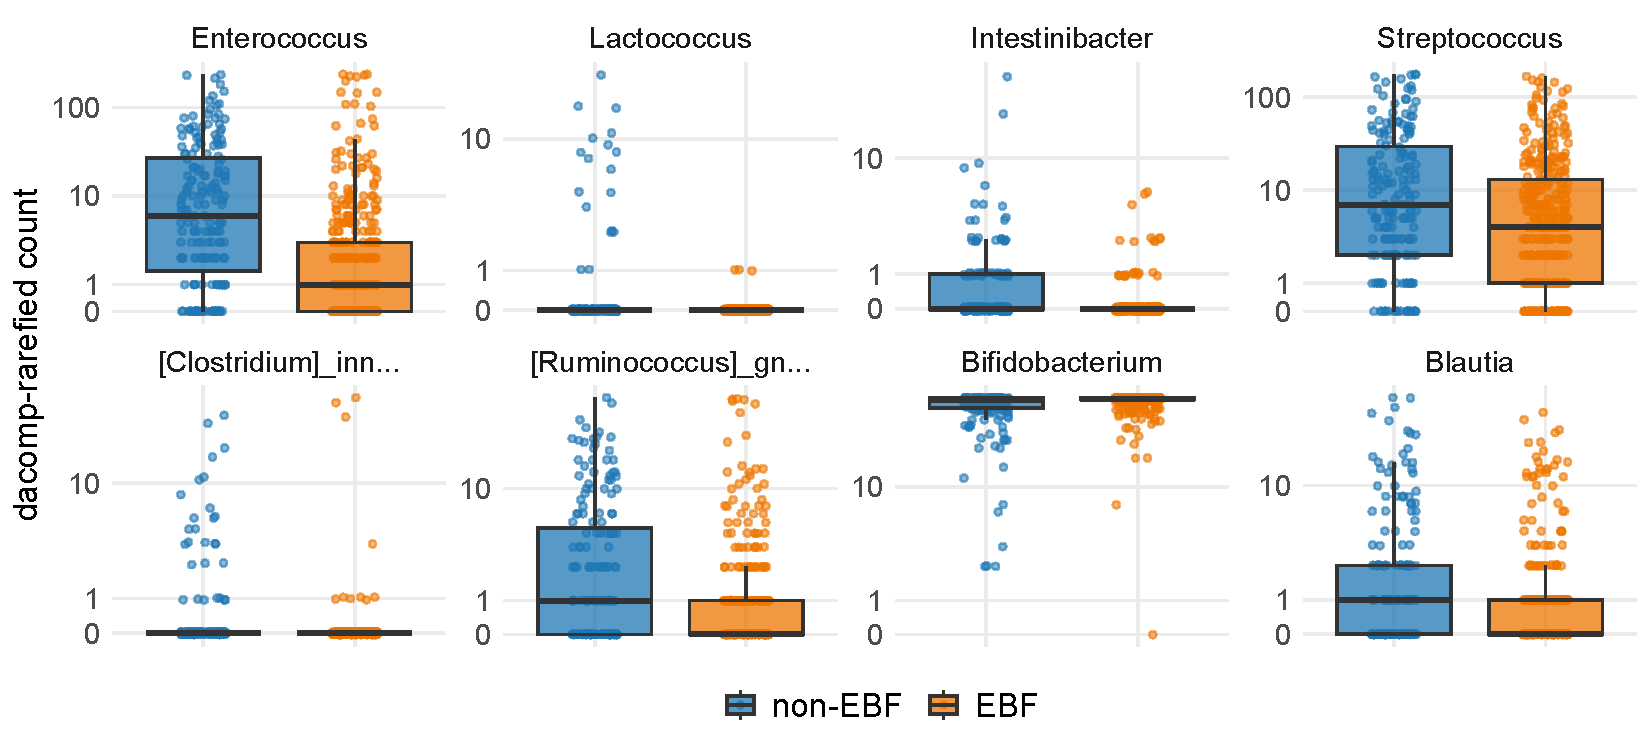
\includegraphics[width=\textwidth]{../ch07_application/figures/08_diff_abundance/thesis_rarefied_count_boxplots_with_zeros-1.pdf}
\caption{\label{fig:7app:da:rarefied-boxplots}\textbf{DACOMP-rarefied counts for selected genera.} Boxplots show group-wise DACOMP-rarefied counts for the eight genera highlighted in the differential abundance volcano plot. Points represent individual samples. The y-axis is displayed on a logarithmic scale, while the axis labels show the original count values. The plot is descriptive and illustrates the group-wise count patterns underlying the DACOMP test statistics.}
\end{figure}

%%%%%%%%%%%%%%%%%%%%%%%%%%%%%%%%%%%%%
\section{Differential distribution analysis}
\label{sec:7app:differential-distribution}
%%%%%%%%%%%%%%%%%%%%%%%%%%%%%%%%%%%%%

%====================================
\subsection{Analysis setup and adapted \texttt{waddR} workflow}
\label{sec:7app:differential-distribution:setup}
%====================================

The differential abundance analysis in the previous section focused on relative abundance shifts of individual genera. As a complementary feature-level analysis, we next assessed whether the marginal distributions of individual genera differed between the two EBF groups. This analysis was performed using the Wasserstein-based \texttt{waddR} framework introduced in Section~\ref{sec:4feature:diffdist}. In contrast to differential abundance testing, differential distribution testing is sensitive not only to location shifts, but also to differences in variability, tail behavior, zero prevalence, and more general distributional shape. The analysis used the binary EBF contrast and the default genus-level data set defined in Section~\ref{sec:7app:default_data}, comparing children without EBF ($n=179$) with children with EBF duration $\ge 2$ months ($n=375$).

Two differential distribution analyses were conducted. The first analysis followed the adapted two-stage approach described in Section~\ref{sec:4feature:diffdist_waddr_microbiome}. In this approach, the zero component was defined on the original count scale and tested whether the prevalence of zero counts differed between the two EBF groups. The non-zero component used the squared 2-Wasserstein statistic on CLR-transformed values, but only among samples in which the corresponding genus had a positive original count. Thus, original counts determined whether an observation entered the non-zero stage, whereas CLR coordinates defined the distributional values being compared. The $p$-values from the zero and non-zero components were combined using Fisher's method to be in line with the original \texttt{waddR} approach. Only the non-zero Wasserstein component was refined using \texttt{permApprox}, because this is the permutation-based part for which the observed and permuted Wasserstein statistics are available.

The second analysis was a one-stage complete-CLR approach. Here, \texttt{waddR} was applied directly to the complete CLR-transformed distributions, including samples with original zero counts through their multiplicative-replacement CLR values. This analysis does not separate zero prevalence from the remaining distributional shape. It is therefore less aligned with the two-stage interpretation of \texttt{waddR}, but it provides a useful contrast because it tests the full CLR-coordinate distribution in a single Wasserstein test. It also makes the connection to the zero-$p$-value problem visible, because all original zeros remain part of the distribution through their replaced CLR values.

For the \texttt{permApprox} refinements, $p$-value approximation was performed as a right-tailed problem, since larger Wasserstein statistics indicate stronger evidence against equality of distributions. The default \texttt{permApprox} configuration described in Section~\ref{sec:6perm:workflow:default_config} was used, with one modification: the approximation threshold was set to $0.01$. This choice was made to align the refinement step with the original \texttt{waddR} tail-approximation rule, which fits a GPD when fewer than $10$ exceedances are observed among $999$ permutations. Thus, the empirical \texttt{waddR} $p$-values were retained outside the extreme tail, whereas small Wasserstein $p$-values were refined by constrained GPD approximation.

%====================================
\subsection{Zero $p$-values and constrained tail approximation}
\label{sec:7app:differential-distribution:zero-pvalues}
%====================================

In the single-cell application of the \texttt{permApprox} study, the original \texttt{waddR} tail approximation produced a considerable number of zero $p$-values \citep{peschel2026permapprox}. In that setting, zero $p$-values arose for two different reasons: some were caused by numerical rounding, whereas others were caused by bounded GPD support under negative shape estimates. The latter case cannot be resolved by numerical post-processing alone and motivated the support-constrained GPD approximation described in Chapter~\ref{ch:permapprox}. In the present PASTURE analysis, this behavior was less pronounced, most likely because the microbiome application has substantially fewer tests and less extreme tail probabilities than the single-cell example.

In the adapted two-stage analysis, no zero $p$-values were observed for the non-zero Wasserstein component. In the one-stage complete-CLR analysis, however, \texttt{waddR} returned zero $p$-values for $5$ of the $116$ taxa for which a finite $p$-value was available, and one additional NA $p$-value. Recomputing the tail $p$-values from the exported observed and permuted Wasserstein statistics with constrained \texttt{permApprox} yielded finite, non-zero $p$-values for all $117$ taxa.


Figure~\ref{fig:7app:dd:pvalue-comparison} shows this zero-$p$-value diagnostic for the one-stage complete-CLR analysis. The left panel shows the $p$-values returned by \texttt{waddR}, including five zero $p$-values and one NA value. The right panel shows the corresponding $p$-values after constrained \texttt{permApprox} refinement. The originally zero and NA values are resolved, and no zero $p$-values remain. This provides a small but relevant example of the zero-$p$-value problem discussed in Chapter~\ref{ch:permapprox}, and illustrates how the constrained GPD approximation can be used to obtain finite tail probabilities for the same observed and permuted test statistics.

\begin{figure}[!htb]
\centering
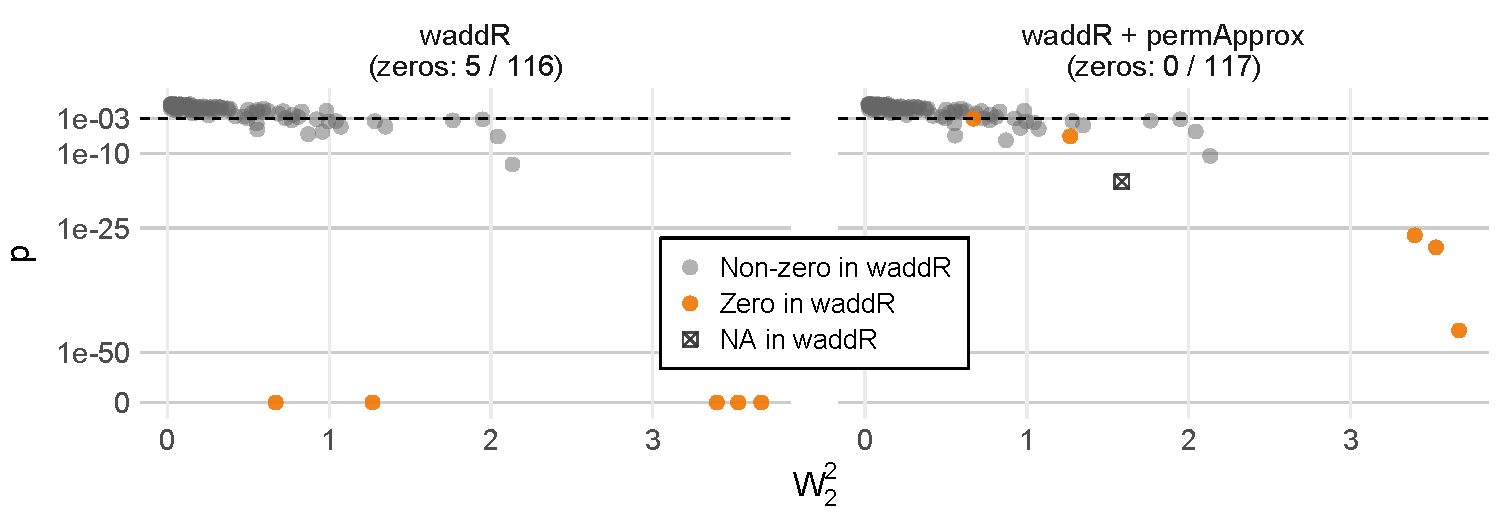
\includegraphics[width=\textwidth]{../ch07_application/figures/09_diff_distribution/thesis_pvalues_complete_clr_waddr_permapprox_constrained_only-1.pdf}
\caption{\label{fig:7app:dd:pvalue-comparison}\textbf{Comparison of \texttt{waddR} and constrained \texttt{permApprox} $p$-values for the one-stage complete-CLR analysis.} Each point represents one genus. The x-axis shows the observed squared 2-Wasserstein statistic $W_2^2$, and the y-axis shows the raw $p$-value on a logarithmic scale. The left panel shows $p$-values returned by \texttt{waddR}, and the right panel shows $p$-values obtained by constrained \texttt{permApprox} refinement from the same observed and permuted Wasserstein statistics. The dashed horizontal line marks the empirical lower bound $1/(B+1)$ for $B=999$ permutations. Zero $p$-values are mapped to the lower plotting boundary for visualization.}
\end{figure}

%====================================
\subsection{Differential distribution results}
\label{sec:7app:differential-distribution:results}
%====================================

The differential distribution results are summarized in Figure~\ref{fig:7app:dd:volcano}. In contrast to a classical volcano plot based on a single effect statistic, each panel displays the native statistic of the corresponding \texttt{waddR} component on the x-axis. For the non-zero \text{distribution} component and the complete-CLR analysis, this is the squared 2-Wasserstein statistic $W_2^2$, and the displayed $p$-values are constrained \texttt{permApprox}-refined $p$-values. For the zero-prevalence component, the x-axis shows the absolute zero-stage statistic $|Z_0|$. For the combined two-stage result, the x-axis shows the combined statistic $C$ obtained from Fisher's method. The y-axis shows the corresponding raw $p$-values on the $-\log_{10}$ scale, while point colors indicate significance after Benjamini--Hochberg adjustment at $\alpha=0.01$. The number of testable taxa differs between panels because not all component statistics could be computed for all genera. For example, \emph{Coprobacillus} had only zero counts in one EBF group and therefore no non-zero Wasserstein statistic. This pattern is instead represented in the zero-prevalence component. Conversely, \emph{Bifidobacterium} had no zero counts and therefore no zero-stage statistic.

The non-zero distribution component identified $15$ of $116$ testable genera as significant after adjustment. These signals include several genera that were already prominent in the differential abundance analysis, such as \emph{Intestinibacter}, \emph{Enterococcus}, \emph{Blautia}, \emph{Streptococcus}, and the \emph{[Ruminococcus] gnavus group}. The zero-prevalence component identified $5$ of $116$ testable genera, including \emph{Lactococcus}, \emph{Haemophilus}, \emph{Leuconostoc}, \emph{Terrisporobacter}, and \emph{Lactobacillus}. Combining the two components yielded $20$ significant genera among $115$ testable genera. Thus, the adapted two-stage result separates distributional differences among originally observed values from differences in the probability of observing a zero count, while the combined statistic summarizes both sources of evidence when both component $p$-values are available.

The one-stage complete-CLR analysis identified $23$ of $117$ genera as significant after adjustment. The strongest signals included \emph{Intestinibacter}, \emph{Enterococcus}, \emph{Lactococcus}, the \emph{[Ruminococcus] gnavus group}, the \emph{[Clostridium] innocuum group}, and \emph{Blautia}. The overlap between the adapted two-stage and complete-CLR approaches indicates that both analyses capture a common set of distributional differences between the EBF groups. At the same time, the approaches are not identical: the two-stage analysis separates zero prevalence from the distribution among originally observed values, whereas the one-stage analysis treats the replaced CLR values of originally zero counts as part of the full distribution. Consequently, the corresponding statistics and $p$-values should not be interpreted as directly interchangeable.

\begin{figure}[!htb]
\centering
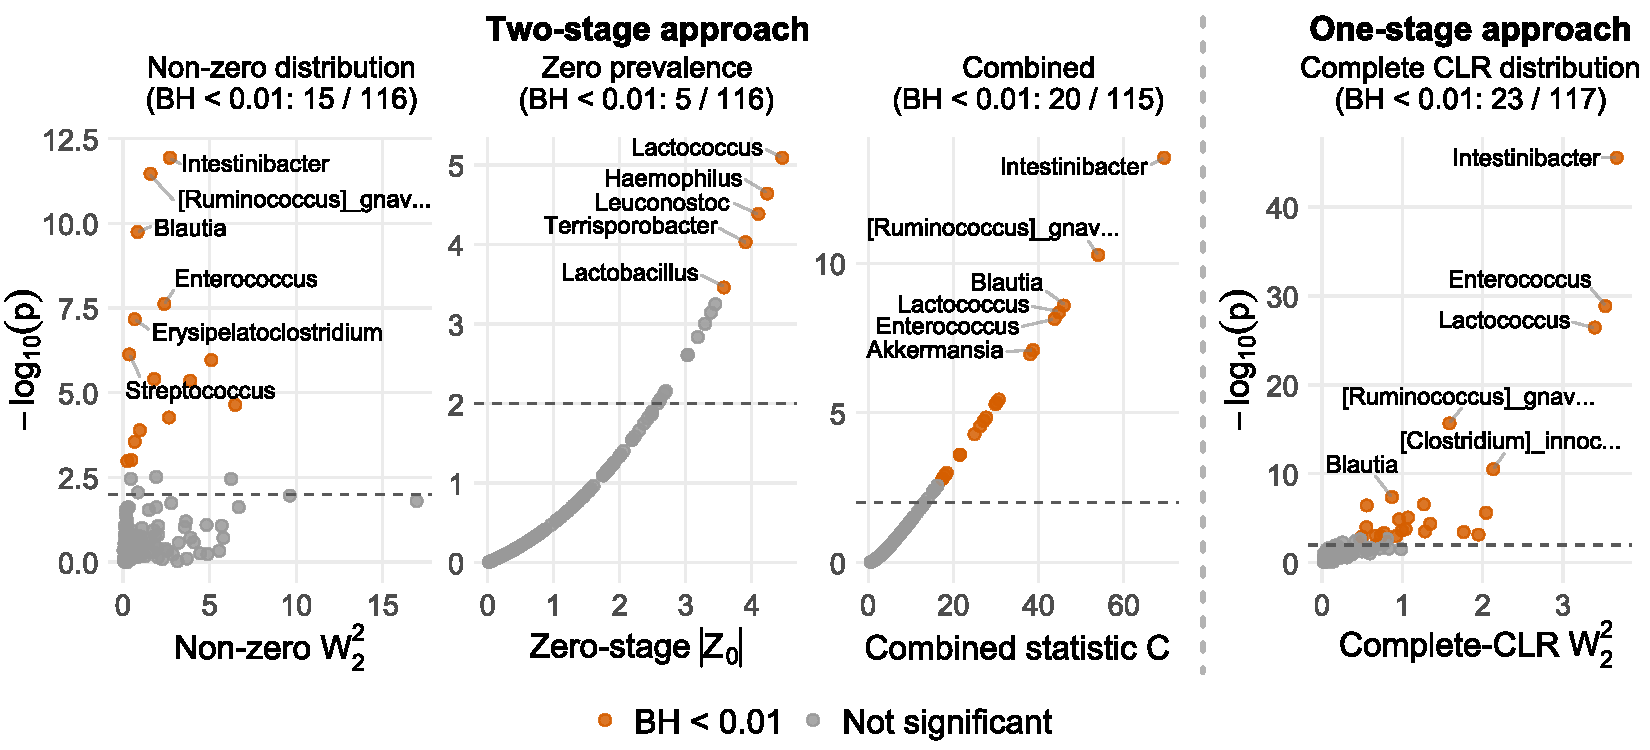
\includegraphics[width=\textwidth]{../ch07_application/figures/09_diff_distribution/thesis_volcano_two_stage_one_stage_native-2.pdf}
\caption{\label{fig:7app:dd:volcano}\textbf{Differential distribution analysis with adapted two-stage and one-stage \texttt{waddR} approaches.} The first three panels show the adapted two-stage approach: the non-zero distribution component, the zero-prevalence component, and the combined result. The fourth panel shows the one-stage complete-CLR analysis. The x-axis displays the native statistic of the respective test component: the squared 2-Wasserstein statistic $W_2^2$ for the non-zero distribution and complete-CLR analyses, the absolute zero-stage statistic $|Z_0|$ for the zero-prevalence analysis, and the combined statistic $C$ for the combined two-stage result. For the two Wasserstein-based panels, $p$-values are constrained \texttt{permApprox}-refined $p$-values. The y-axis shows raw $p$-values on the $-\log_{10}$ scale. Orange points indicate taxa with Benjamini--Hochberg-adjusted $p$-values below $\alpha=0.01$ within the respective panel, and grey points indicate non-significant taxa. The dashed horizontal line marks $\alpha=0.01$ for visual reference. Panel subtitles report the number of significant taxa and the number of taxa for which the respective statistic and $p$-value could be computed. The totals differ between panels because some component statistics are undefined for taxa with only zero counts in one group or no zero counts at all.}
\end{figure}

The adjusted $p$-values for the adapted two-stage components, the combined two-stage analysis, and the one-stage complete-CLR analysis are reported in Appendix Table~\ref{tab:app:7app:diff_distribution_pvalues_all_approaches}. The table confirms the visual impression from Figure~\ref{fig:7app:dd:volcano}: the strongest combined two-stage signals are dominated by genera that also appeared in the differential abundance analysis, but the differential distribution analysis additionally highlights whether the signal is driven by the non-zero distribution, by zero prevalence, or by both. This distinction is useful because a genus can show a similar abundance shift in a differential abundance analysis while differing in the distributional mechanism that produces this shift.

%====================================
\subsection{Distribution diagnostics for selected genera}
\label{sec:7app:differential-distribution:diagnostics}
%====================================

To further inspect the strongest distributional signals, Figure~\ref{fig:7app:dd:diagnostics} shows distribution diagnostics for the four genera with the smallest constrained \texttt{permApprox} $p$-values in the one-stage complete-CLR analysis. The top row shows histograms of CLR coordinates by EBF group, the middle row shows empirical quantile functions, and the bottom row shows the corresponding permutation distributions of the squared Wasserstein statistic. For \emph{Intestinibacter}, \emph{Enterococcus}, \emph{Lactococcus}, and the \emph{[Ruminococcus] gnavus group}, the observed test statistic lies far in the right tail of the permutation distribution. The histograms and quantile functions show that the group differences are not restricted to a single location shift, but also involve differences in the shape and upper tail of the CLR-coordinate distributions. In particular, the non-EBF group tends to show a stronger upper tail for these genera, which is consistent with the differential abundance results and with the exploratory CLR-coordinate visualizations in Section~\ref{sec:7app:feature-level-exploration}.

\begin{figure}[!htb]
\centering
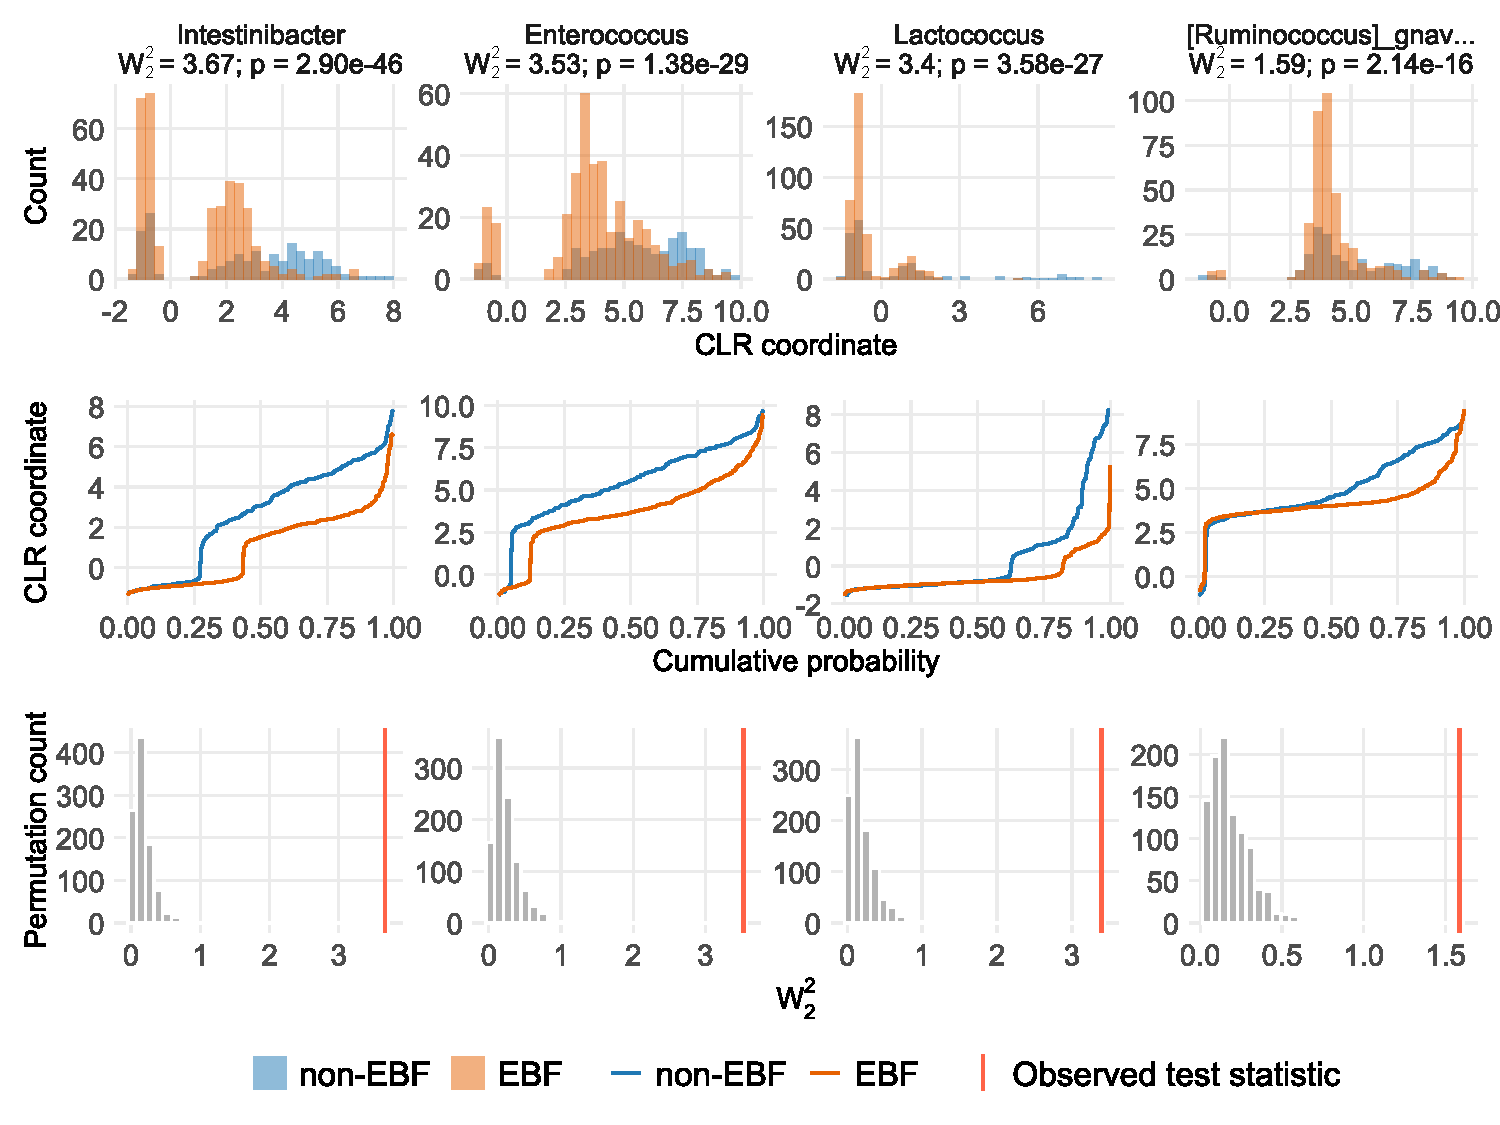
\includegraphics[width=\textwidth]{../ch07_application/figures/09_diff_distribution/thesis_selected_taxa_complete_clr_distribution_diagnostics-2.pdf}
\caption{\label{fig:7app:dd:diagnostics}\textbf{Distribution diagnostics for selected genera in the one-stage complete-CLR analysis.} The figure shows the four genera with the smallest constrained \texttt{permApprox} $p$-values in the one-stage complete-CLR differential distribution analysis. The top row shows histograms of CLR coordinates by EBF group, the middle row shows empirical quantile functions, and the bottom row shows permutation distributions of the squared 2-Wasserstein statistic $W_2^2$. Red vertical lines indicate the observed test statistics. Panel titles report the observed $W_2^2$ statistic and the constrained \texttt{permApprox} $p$-value.}
\end{figure}

%%%%%%%%%%%%%%%%%%%%%%%%%%%%%%%%%%%%%
\section{Network analysis}
\label{sec:7app:networks}
%%%%%%%%%%%%%%%%%%%%%%%%%%%%%%%%%%%%%

The preceding analyses identified genera whose abundance, zero prevalence, or transformed marginal distribution differed between children without EBF and children with EBF duration of at least two months, again referred to as ``non-EBF'' and ``EBF'' groups. These results describe which individual genera show feature-level differences between the two EBF groups, but microbial communities are not merely collections of separate individuals. Genera occur within a joint ecological environment in which their abundances may correlate with those of other community members. Association network analysis addresses this relational aspect by representing genera as nodes and their estimated associations as edges. It thereby shifts attention from marginal, taxon-wise differences to the relationships between genera within the microbial community.

The analysis begins with a baseline network constructed from the complete data set, followed by a comparison of networks estimated separately for the EBF and non-EBF group. Analyzing the baseline network allows us to identify genera with pronounced estimated associations in the complete data set and to characterize the overall network structure of the microbial community. The group comparison assesses whether individual associations or broader network characteristics differ between the EBF groups. In both analyses, we revisit genera highlighted in the preceding sections: we examine whether highly abundant genera occupy notable positions or show distinctive local connectivity in the baseline network, and whether genera with differential abundance or differential distribution are also involved in differential associations between the EBF groups. Such overlap may provide an informative synthesis across analysis targets, although differential abundance or distribution does not imply differential association.

%====================================
\subsection{Baseline association network}
\label{sec:7app:network:baseline}
%====================================

The baseline network was constructed from the complete default data set introduced in Section~\ref{sec:7app:default_data}, which comprises $117$ genera and $592$ samples. Network construction was performed with \texttt{NetCoMi}'s \texttt{netConstruct()} function. As in the preceding analyses, counts were transformed to relative abundances, zeros were replaced by multiplicative replacement, and the resulting compositions were CLR-transformed. Conditional associations were estimated with SPIEC-EASI using the Meinshausen--Bühlmann neighborhood-selection approach described in Section~\ref{sec:5net:net_constr:spieceasi}. A sequence of $30$ regularization parameters was considered, and the final regularization level was selected by the Stability Approach to Regularization Selection using $30$ subsamples and a stability threshold of $0.1$. The directed neighborhood estimates were symmetrized using the average of the two corresponding regression coefficients. The resulting edge weights are therefore symmetrized MB regression coefficients rather than partial correlations. In the following, they are referred to as estimated associations. Their signs indicate the direction of the estimated conditional association, whereas their magnitudes remain specific to the regression-coefficient scale. Because SPIEC-EASI estimates a sparse conditional-dependence structure and selects the regularization level internally by StARS, no additional sparsification was applied.

Figure~\ref{fig:7app:network:association_distribution} summarizes the estimated association matrix. Of the $\binom{117}{2} = 6786$ possible genus pairs, $124$ received a non-zero estimated association, whereas the remaining $6662$ pairs were set to zero by the SPIEC-EASI procedure. The resulting network is therefore sparse, with an edge density of approximately $1.8\%$. The non-zero estimated associations are predominantly positive and modest in magnitude, while negative associations occur less frequently.

\begin{figure}[!htb]
\centering
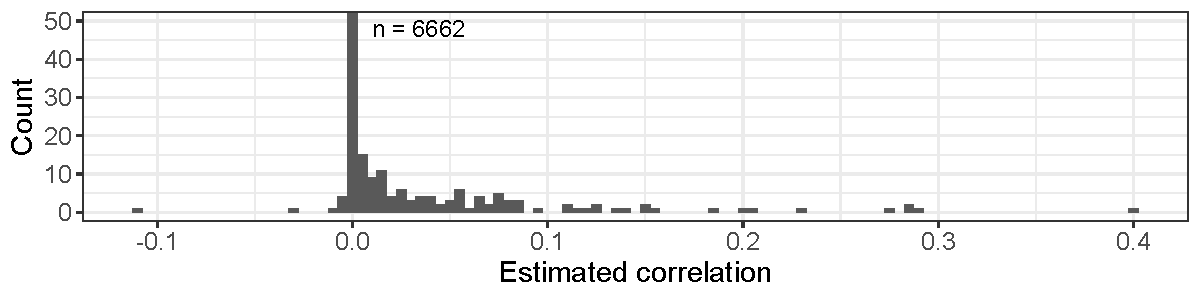
\includegraphics[width=\textwidth]{../ch07_application/figures/10_network_analysis/thesis_single_association_histrogram-1.pdf}
\caption{\textbf{Distribution of estimated associations in the baseline network.} The histogram shows the distribution of estimated associations, including the zero-valued entries resulting from SPIEC-EASI sparsification. The annotation reports the number of associations estimated as zero by the sparsity-inducing procedure.}
\label{fig:7app:network:association_distribution}
\end{figure}

The resulting network was analyzed with \texttt{netAnalyze()} to compute global and node-level characteristics, including component structure, centrality measures, and hub taxa. Figure~\ref{fig:7app:network:baseline_network}, created with \texttt{NetCoMi}'s \texttt{plot()} function, provides an initial visual summary of these characteristics. Node colors represent phylum rather than the detected network clusters because the clustering primarily separates the disconnected components and would therefore add little information beyond the graph layout. Node sizes are proportional to the mean CLR coordinate across samples and therefore summarize the average relative log-ratio abundance of each genus on the transformed scale.

The network consists of one large connected component as well as several smaller components on the right-hand side of the plot. In addition, $31$ of the $117$ genera are singletons. To improve readability, singleton genera are omitted from the visualization unless they are explicitly labeled. The degree distribution shown in Figure~\ref{fig:7app:network:degree_distribution} confirms the heterogeneous connectivity apparent in the network plot: most genera have only few connections, whereas a small number of genera have substantially larger degrees. The network is therefore sparse overall, but its connected structure is dominated by a limited set of highly connected nodes.

The hub taxa identified by \texttt{netAnalyze()} were \emph{8\_Comamonadaceae(F)}, \emph{Blastococcus}, \emph{Brevundimonas}, \emph{Lachnospira}, \emph{Lachnospiraceae ND3007 group}, and \emph{Stenotrophomonas}. Hubs were defined as genera with eigenvector centrality above the empirical $95\%$ quantile. Due to their high connectivity, these taxa also occupy central positions in the network plot. Notably, these genera have comparatively small node sizes, corresponding to low mean CLR coordinates. Their apparent network prominence should therefore be interpreted cautiously, because associations among sparse genera may be sensitive to multiplicative zero replacement before CLR transformation.

In contrast, several genera highlighted in the preceding abundance and differential-distribution analyses show only few and comparatively weak estimated associations, and some occur in smaller connected components. \emph{Bifidobacterium} as the most abundant genus has a few edges but does not have a central position in the network. Its three negative associations with genera highlighted in the preceding analyses are nevertheless notable and suggest a potential relational pattern that complements the marginal feature-level results. The subsequent network comparison examines whether these associations, hub characteristics, and broader network properties differ when the data are analyzed separately for the two EBF groups.

\begin{figure}[H]
\centering
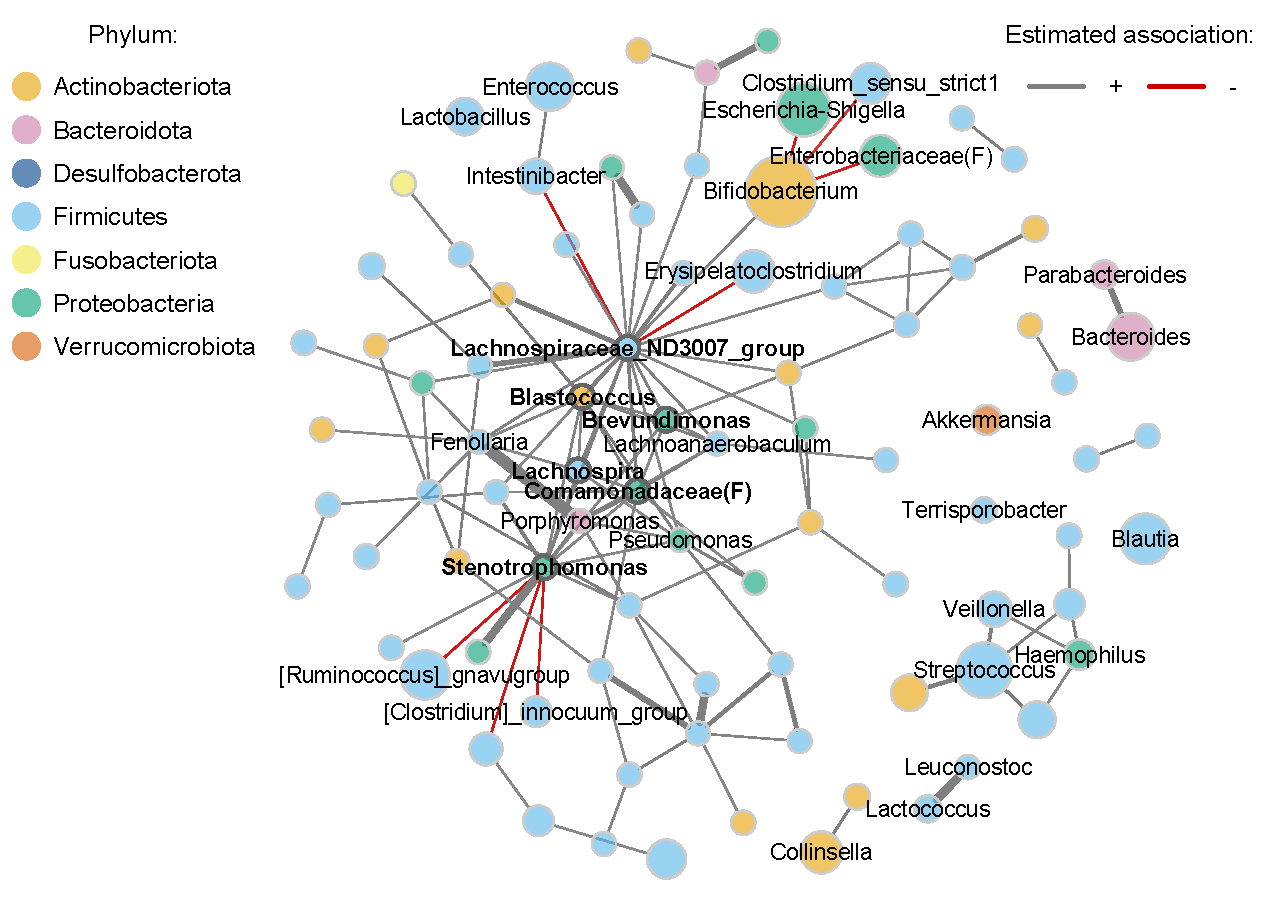
\includegraphics[width=\textwidth]{../ch07_application/figures/10_network_analysis/thesis_single_net_plot_baseline-1.pdf}
\caption{\textbf{Baseline association network for the complete default data set.} Nodes represent genera and are colored according to phylum. Node sizes are proportional to the mean CLR coordinate across samples. Gray and red edges indicate positive and negative estimated SPIEC-EASI associations, respectively. Labels identify highly abundant genera, genera highlighted in the differential abundance or differential distribution analyses, genera with high eigenvector centrality, and the three genera negatively associated with \emph{Bifidobacterium}.}
\label{fig:7app:network:baseline_network}
\end{figure}

\begin{figure}[H]
\centering
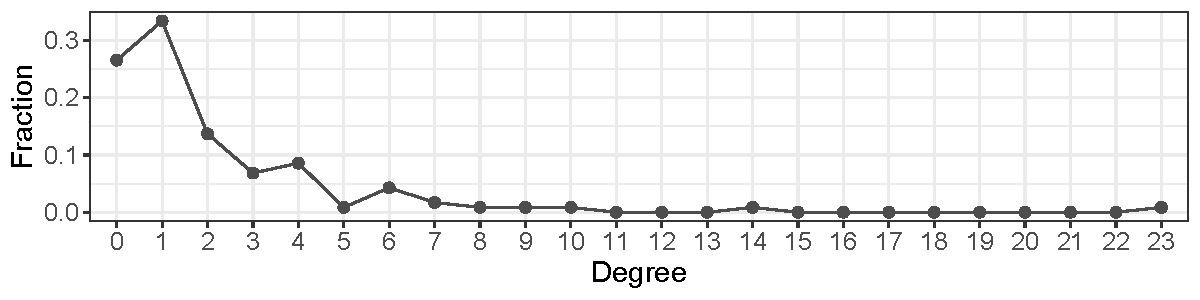
\includegraphics[width=\textwidth]{../ch07_application/figures/10_network_analysis/thesis_single_degree_distribution-1.pdf}
\caption{\textbf{Degree distribution of the baseline association network.} The degree of a genus is the number of genera to which it is connected, i.e., has a non-zero estimated association.}
\label{fig:7app:network:degree_distribution}
\end{figure}

\begin{figure}[H]
\centering
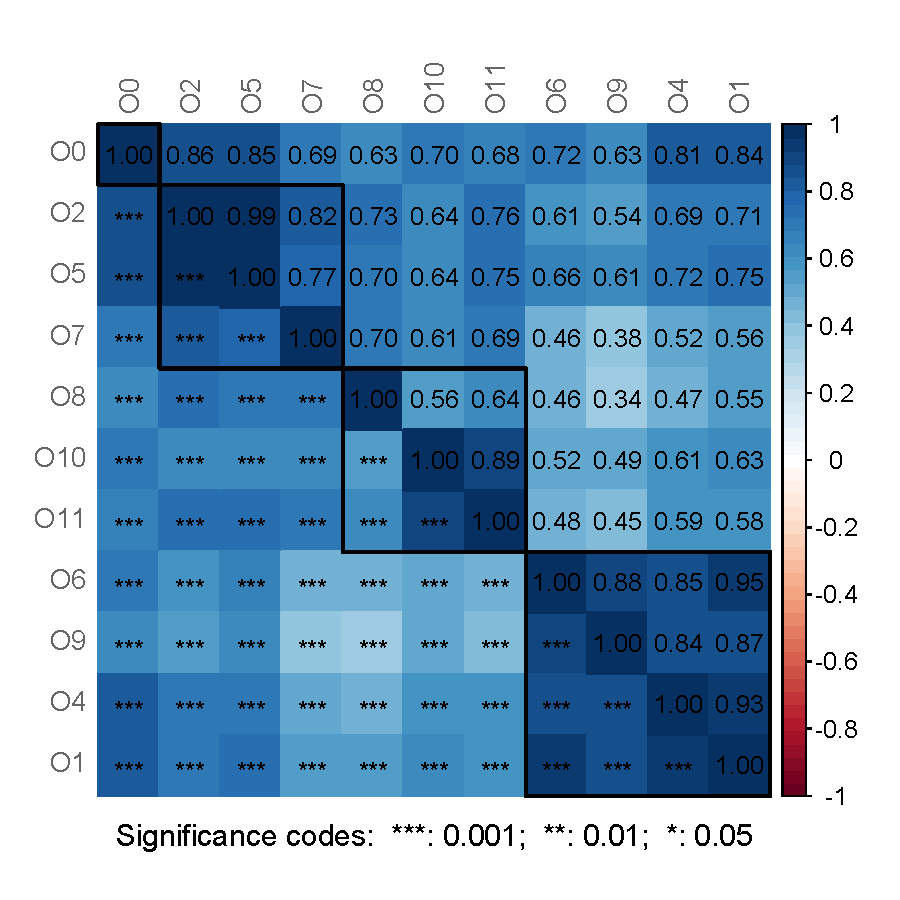
\includegraphics[width=0.9\textwidth]{../ch07_application/figures/10_network_analysis/thesis_single_gcm-1.pdf}
\caption{\textbf{Graphlet correlation matrix of the baseline association network.} Entries show Spearman correlations between graphlet orbit counts across genera. Significance symbols refer to tests of non-zero correlation performed with Fisher's z-test.}
\label{fig:7app:network:baseline_gcm_heatmap}
\end{figure}

Finally, Figure~\ref{fig:7app:network:baseline_gcm_heatmap} shows the corresponding graphlet correlation matrix (GCM). The matrix is dominated by strong positive correlations between graphlet orbit counts, indicating that genera participating frequently in one orbit also tend to participate frequently in several others. Compared with the GCMs of the standard networks shown in Figures~\ref{fig:5net:net_analysis:gcm_example} and \ref{fig:app:5net:gcm_network_models}, the PASTURE GCM is most similar overall to the standard Barabási--Albert (BA) network. This is notable because the modified BA network in Figure~\ref{fig:5net:net_analysis:gcm_example} was deliberately augmented with peripheral nodes to obtain a structure that appears more similar to empirical networks. In that modified network, the additional peripheral nodes weaken the correlations of certain peripheral orbit roles, in particular O6 and O9, with the remaining orbit counts. However, the local role of peripheral nodes differs between the two networks. In the modified BA network, the added peripheral nodes frequently occur in triangle- and star-related graphlets, which weakens the correlations of orbits O6 and O9 to other orbits. In the PASTURE network, by contrast, peripheral genera more often occupy endpoint positions in chain-like graphlets. 

The PASTURE GCM also shares some features with the stochastic block model, including pronounced positive correlations among orbit counts in the lower-right part of the matrix. At the same time, the strong correlation block involving O0, O2, O5, and O7 is more pronounced in the stochastic block model heatmap than that of the PASTURE network. Thus, the PASTURE GCM combines features visible in several standard network models, however, these similarities should not be interpreted as evidence that the microbial association network follows a particular generative network model. Rather, the GCM provides a descriptive summary of local network structure that complements the degree and centrality measures and serves as an additional reference for the subsequent comparison of the EBF-group-specific networks.

%====================================
\subsection{Sensitivity to network-construction choices}
\label{sec:7app:network:sensitivity}
%====================================

The baseline network revealed several pronounced estimated associations among genera with low mean CLR coordinates. As these genera were also characterized by high zero fractions before we replaced them, their apparent network prominence may be sensitive to choices made during preprocessing. We therefore examined how the estimated network changes under alternative preprocessing and association-estimation approaches. First, we considered stronger prevalence filters, which remove low-prevalence genera before network construction and allow us to assess which associations among the remaining genera are retained. Second, we compared alternative zero-replacement procedures as a less restrictive approach to handling sparse taxa. Finally, we consider alternative association-estimation methods to investigate how strongly the estimated network depends on the selected measure.

Throughout this subsection, the network constructed in Section~\ref{sec:7app:network:baseline} is used as the baseline network. To facilitate visual comparison, all alternative networks use the same node layout and labeling as the baseline network whenever the corresponding genera are retained.

%------------------------------------
\subsubsection{Prevalence filtering}
\label{sec:7app:network:sensitivity:prevalence}
%------------------------------------

The baseline network was constructed after applying the $1\%$ prevalence filter. Figure~\ref{fig:7app:network:combined_prevalence} compares this network with networks estimated after applying more stringent prevalence filters of $5\%$ and $10\%$. The same preprocessing, SPIEC-EASI MB estimation procedure, and StARS-based regularization selection were used in all three analyses. Only the set of retained genera differed.

The more stringent filters remove the low-prevalence genera that formed several of the highly connected regions in the baseline network. Consequently, these genera and their estimated associations no longer appear in the networks constructed after $5\%$ and $10\%$ filtering. At the same time, several associations among more prevalent genera are recovered. For example, the component centered on \emph{Streptococcus} in the lower-right part of the network remains visible under both stronger filters. Two negative associations involving \emph{Bifidobacterium} are also retained, namely those with \emph{Clostridium sensu stricto 1} and \emph{Enterobacteriaceae(F)}.

The stronger filters therefore reduce the uncertainty associated with associations involving extremely sparse taxa, but this comes at a substantial loss of taxonomic information. Of the $117$ genera retained after $1\%$ filtering, only $58$ remain after applying the $5\%$ filter and $41$ after applying the $10\%$ filter. Thus, stricter filtering yields smaller and visually simpler networks, but it also excludes many genera that may be biologically relevant and that contributed to the structure of the baseline network.

\begin{figure}[!htb]
\centering
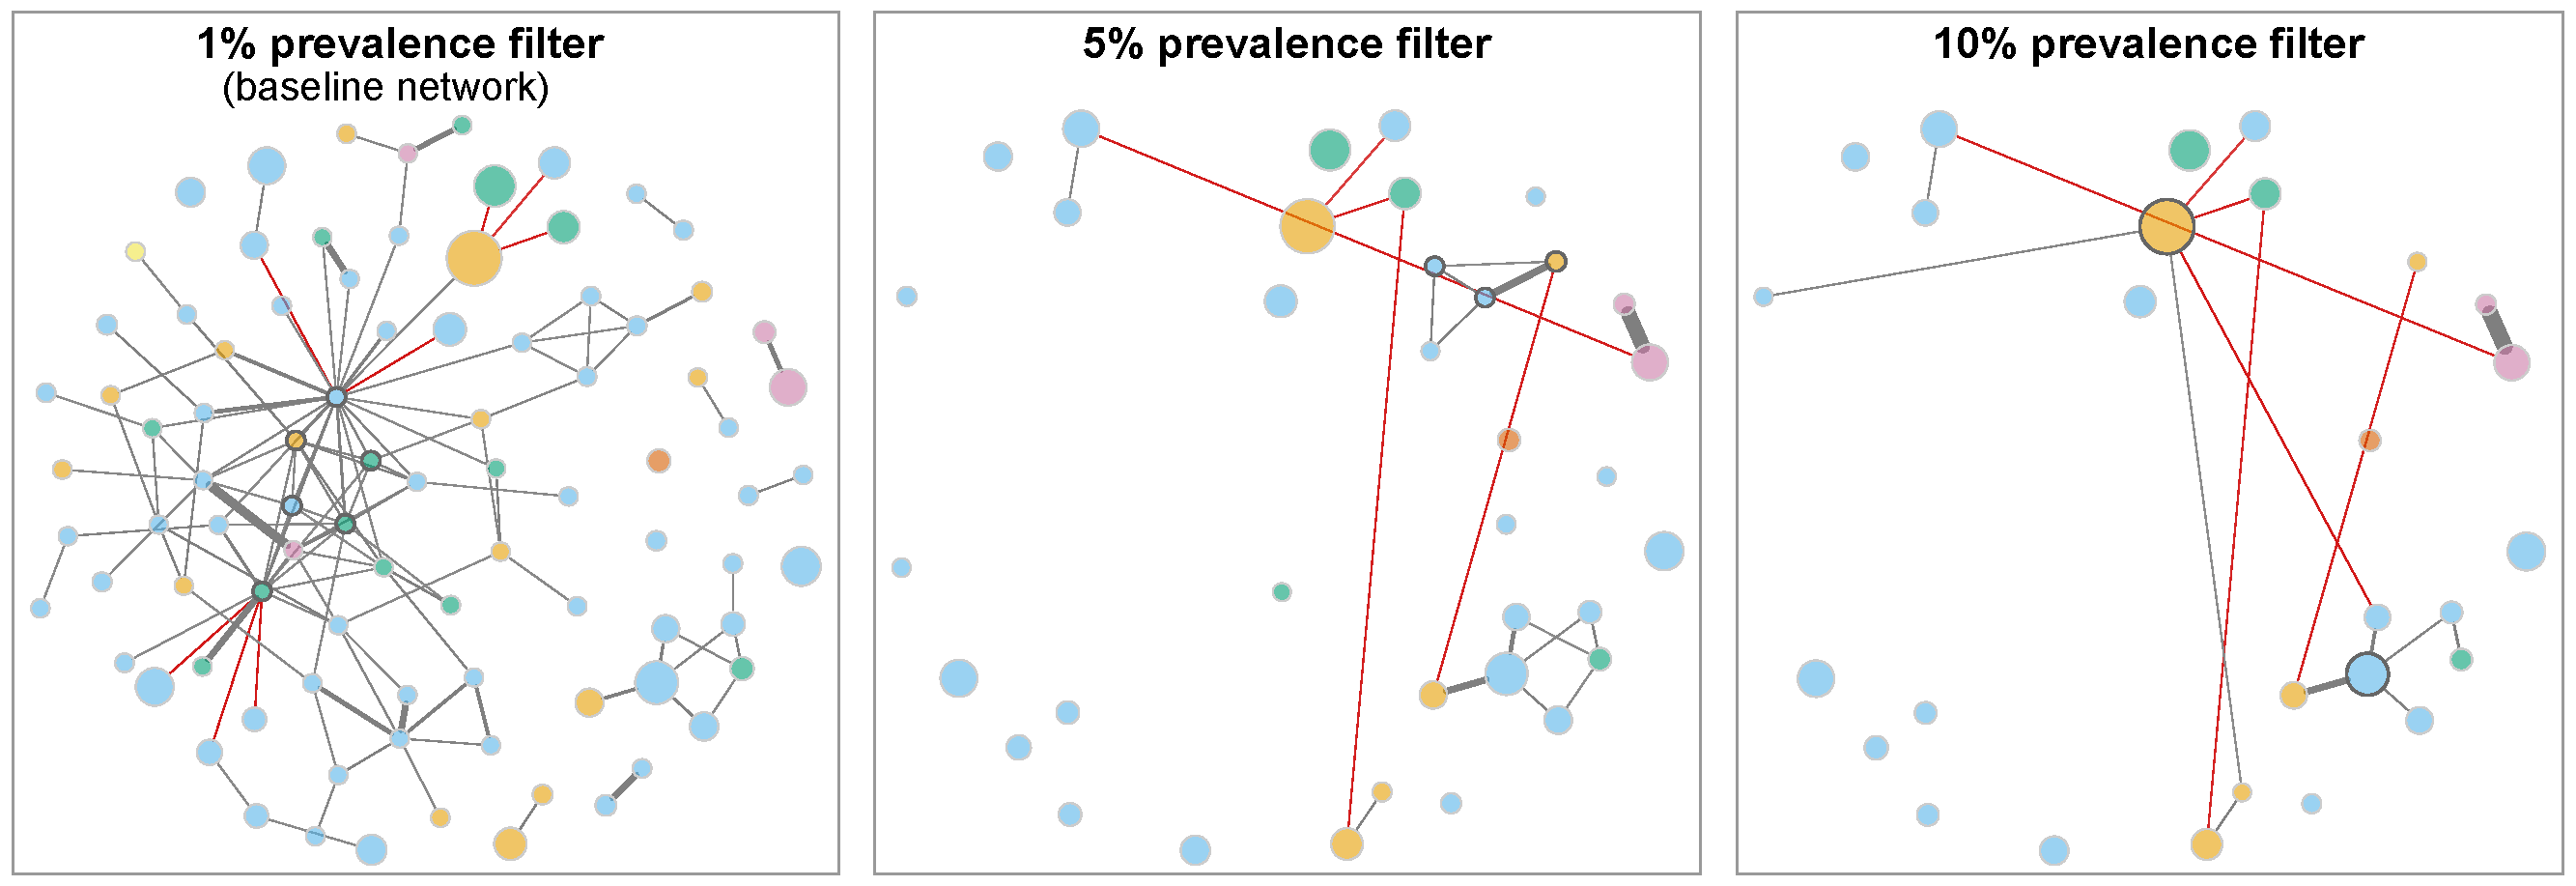
\includegraphics[width=\textwidth]{../ch07_application/figures/10_network_analysis/thesis_combined_networks_prevalence.pdf}
\caption{\textbf{Association networks obtained with different prevalence filters.} Networks were estimated from data filtered at $1\%$, $5\%$, and $10\%$ prevalence using the same preprocessing and SPIEC-EASI MB workflow. The $1\%$ network corresponds to the baseline network. Nodes represent genera and are colored according to phylum, whereas node sizes are proportional to the mean CLR coordinate across samples. Node positions and labels were kept consistent across panels where possible to facilitate comparison. Genera removed by a stricter prevalence filter are not shown in the corresponding network.}
\label{fig:7app:network:combined_prevalence}
\end{figure}

%------------------------------------
\subsubsection{Zero replacement}
\label{sec:7app:network:sensitivity:zero_repl}
%------------------------------------

The baseline network contains several pronounced associations among genera with low mean CLR coordinates and high zero fractions. One possible explanation is that these associations are partly induced by the zero-replacement step preceding CLR transformation. In particular, multiplicative replacement assigns the same small replacement value to zero entries when a common detection limit is used. Genera that are absent in many of the same samples may therefore receive highly similar imputed values, which can affect subsequent association estimation. This possibility cannot be assessed from the baseline network alone. We therefore repeated network construction with three alternative zero-replacement procedures while retaining the $1\%$ prevalence filter, CLR transformation, SPIEC-EASI MB estimation, and all remaining network-construction settings.

As a simple diagnostic approach, zeros were replaced by independently drawn pseudo-counts between zero and the upper bound used for multiplicative replacement, namely $0.65$ times the minimum non-zero relative abundance. Only zero entries were modified. This approach is not intended as a principled imputation method, but deliberately disrupts the common replacement pattern induced by assigning identical pseudo-counts to zero entries. As shown in the left panel of Figure~\ref{fig:7app:network:combined_zero_repl}, the dense region of associations among low-abundance genera disappears under this procedure. This result indicates that these associations are sensitive to the particular treatment of zero entries.

\begin{figure}[H]
	\centering
	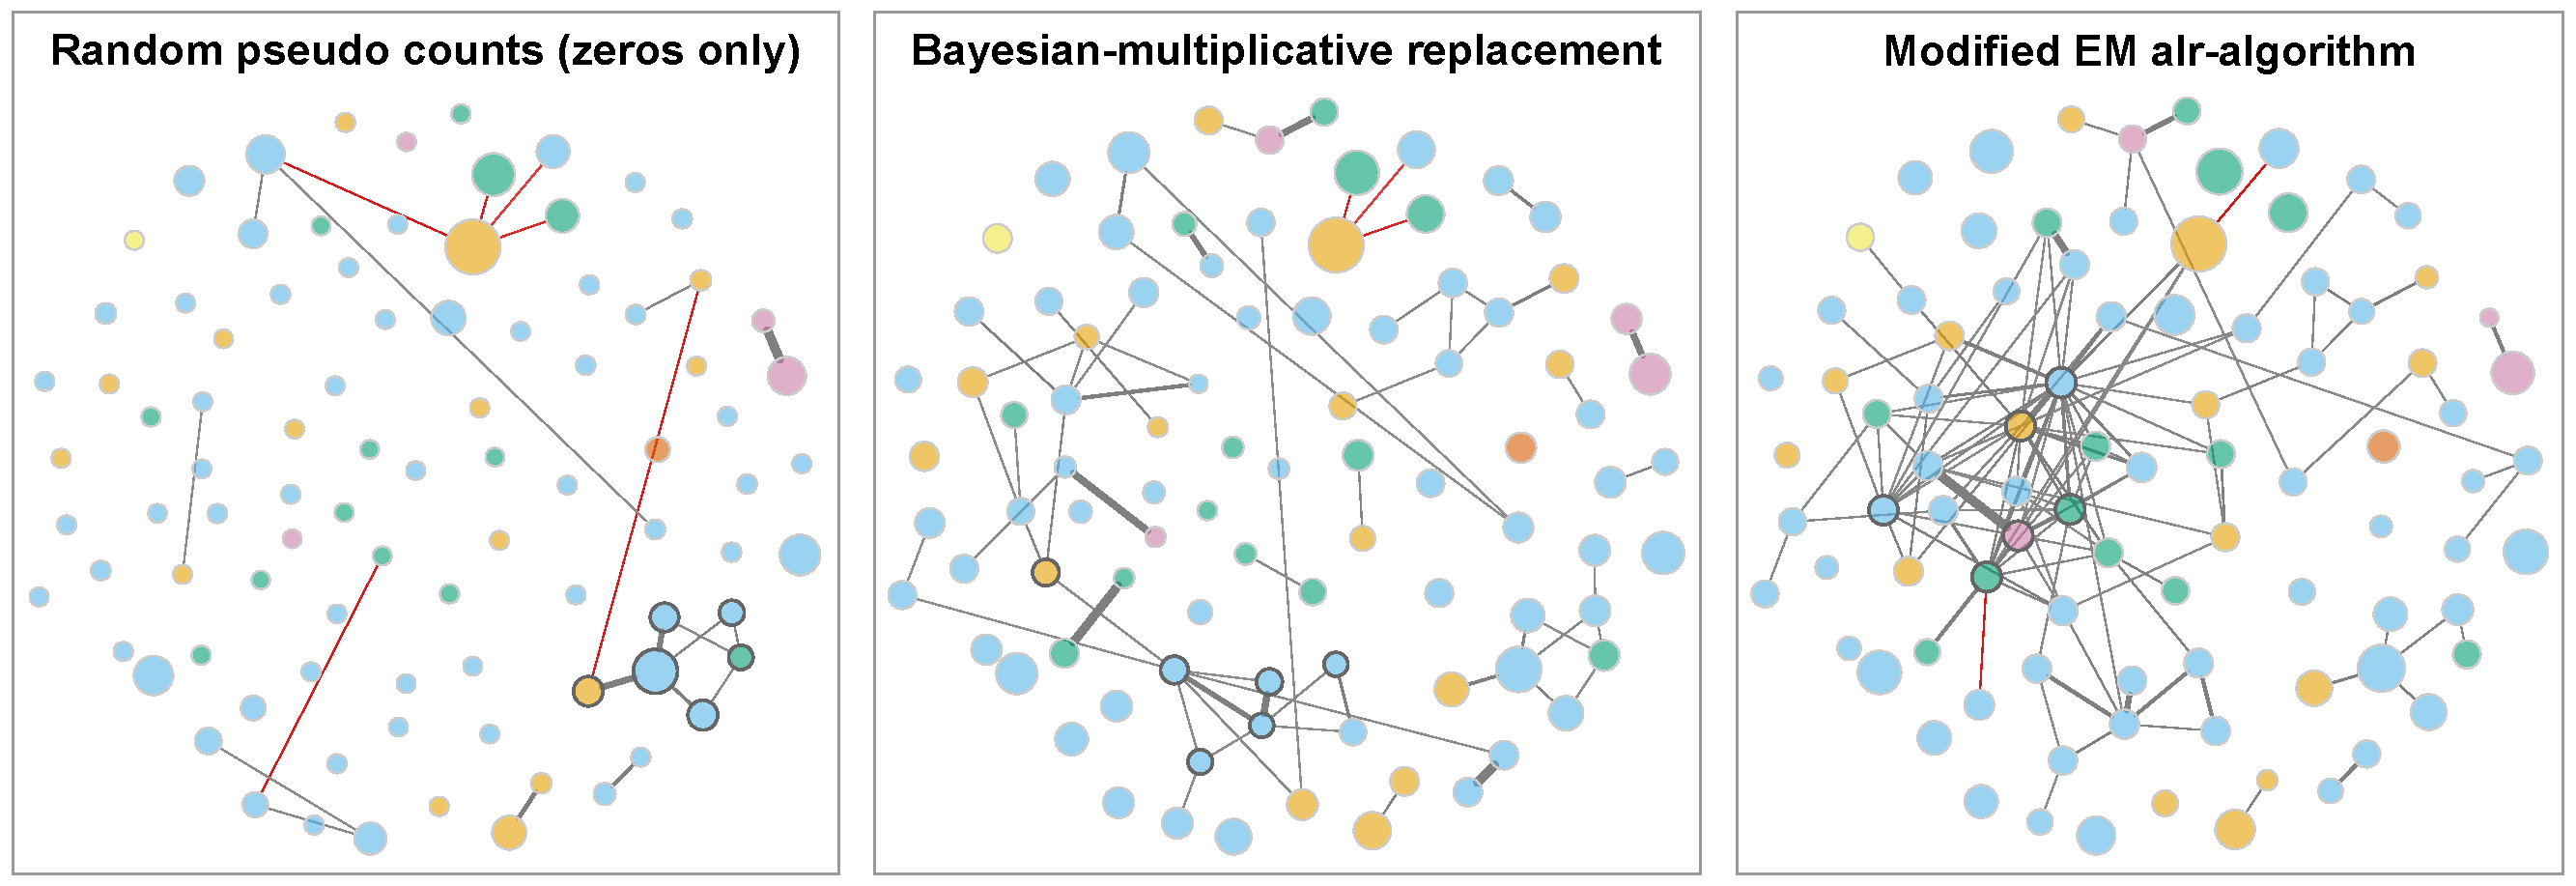
\includegraphics[width=\textwidth]{../ch07_application/figures/10_network_analysis/thesis_combined_networks_zero_repl.pdf}
	\caption{\textbf{Association networks obtained with alternative zero-replacement procedures.} All networks were constructed from the data set filtered at $1\%$ prevalence using CLR transformation and the same SPIEC-EASI MB workflow as for the baseline network. The panels show results after random pseudo-count replacement of zero entries, Bayesian-multiplicative replacement, and the modified EM alr-algorithm, respectively. Nodes represent genera and are colored according to phylum, whereas node sizes are proportional to the mean CLR coordinate across samples. Node positions and labels were kept consistent with the baseline network where possible to facilitate comparison.}
	\label{fig:7app:network:combined_zero_repl}
\end{figure}


The second approach used Bayesian-multiplicative replacement, as described in Section~\ref{sec:2micro:zeros}. This method models the observed counts using a Dirichlet-multinomial framework and derives replacement values from a posterior distribution whose Dirichlet parameters are estimated from the complete count matrix. In contrast to the random pseudo-count approach, it therefore provides a model-based treatment of count zeros while remaining computationally inexpensive. The corresponding network in the center panel of Figure~\ref{fig:7app:network:combined_zero_repl} likewise does not reproduce the highly connected low-abundance region observed in the baseline network. At the same time, several associations among more prevalent genera remain visible, including the component centered on \emph{Streptococcus}.

Finally, the modified EM alr-algorithm described in Section~\ref{sec:2micro:zeros} was applied. This procedure imputes zeros through an expectation-maximization algorithm on additive log-ratio coordinates and explicitly incorporates the estimated covariance structure. Here, it produced a markedly denser network and retained several associations among low-abundance genera, as shown in the right panel of Figure~\ref{fig:7app:network:combined_zero_repl}. Thus, accounting for multivariate dependence during imputation does not necessarily reduce sensitivity to sparse taxa and may itself induce substantial changes in the inferred network.

Overall, the comparison demonstrates that the apparent prominence of low-abundance genera in the baseline network depends strongly on the chosen zero-replacement method. The random pseudo-count and Bayesian-multiplicative approaches weaken this pattern, whereas the modified EM alr-algorithm yields an even denser low-abundance subnetwork. These results do not identify a uniquely correct replacement procedure, but they show that associations involving highly sparse genera should be interpreted cautiously. The next subsection therefore examines whether this sensitivity persists when the association-estimation method itself is changed.


We additionally considered a variant of multiplicative replacement in which the detection limit was determined separately for each sample rather than globally across the complete data set. Specifically, the replacement value in each sample was based on $0.65$ times the smallest non-zero relative abundance observed in that sample. The corresponding network is not shown here but is provided in the thesis repository. This analysis produced an even denser subnetwork among the low-abundance hub taxa than the baseline procedure. Such behavior is consistent with the fact that the replacement value now varies across samples and is partly determined by sample-specific sequencing depth and sparsity. When several rare genera are simultaneously absent from the same sample, they receive the same sample-specific replacement value and may therefore share an artificial abundance pattern across samples after CLR transformation. The result further illustrates that associations among highly sparse genera can be strongly affected not only by whether zeros are replaced, but also by how the replacement value is defined.

%------------------------------------
\subsubsection{Association estimation}
\label{sec:7app:network:sensitivity:association}
%------------------------------------

Two further approaches are particularly relevant when the aim is to make network estimation less sensitive to potentially zero-induced spurious associations: the sparse-plus-low-rank (SLR) decomposition proposed by \citet{kurtz2019disentangling} and implemented in \texttt{SpiecEasi}, and SPRING \citep{yoon2019microbial}, which is implemented in an R package of the same name. As explained in Section~\ref{sec:5net:net_construction}, both methods estimate sparse conditional-dependence networks, but they address different potential sources of spurious association. The SLR approach represents the inverse covariance structure as the sum of a sparse component and a low-rank component, where the latter captures variation attributable to a small number of unobserved factors. SPRING, in contrast, estimates a latent correlation matrix under a truncated Gaussian copula model and avoids external zero replacement by using the modified CLR transformation described in Section~\ref{sec:2micro:clr_with_zeros:mCLR}.

For SPIEC-EASI SLR estimation, candidate ranks from $2$ to $5$ were considered for the low-rank component, and the rank minimizing the extended Bayesian information criterion (eBIC) was selected. We used $\gamma = 0.5$, a commonly used conservative default for eBIC-based high-dimensional graph selection. The resulting eBIC values and heatmaps of the fitted low-rank components are provided in the thesis repository. The remaining SPIEC-EASI settings were identical to those of the baseline analysis, with a $\lambda$ path of length $30$, $30$ StARS subsamples, and a stability threshold of $0.1$. For SPRING, the same StARS settings were used. No additional sparsification was applied because both procedures incorporate stability-based model selection.

Figure~\ref{fig:7app:network:combined_association} compares the baseline SPIEC-EASI MB network with the networks estimated using SPIEC-EASI SLR and SPRING. The baseline network is repeated in the left panel to facilitate comparison. Both alternative approaches yield markedly different edge sets from the MB network and from the preceding preprocessing-based sensitivity analyses. In particular, the SLR network contains many negative estimated associations, whereas the SPRING network shows a distinct mixture of positive and negative edges. Importantly, the additional associations in both networks are primarily located among genera with moderate or high mean CLR coordinates rather than among the low-abundance genera that formed the highly connected region of the baseline network. This pattern is consistent with the purpose of both approaches: the SLR model can attribute shared broad-scale variation to the low-rank component, whereas SPRING avoids the common pseudo-value structure introduced by multiplicative zero replacement.

The common layout in Figure~\ref{fig:7app:network:combined_association} is useful for locating differences relative to the baseline network, but it does not necessarily provide the clearest visualization of either alternative network. Network plots based on their respective spring layouts, including the corresponding labels and annotations, are therefore provided in Appendix~\ref{sec:app:7app:net_analysis}.

\begin{figure}[!htb]
\centering
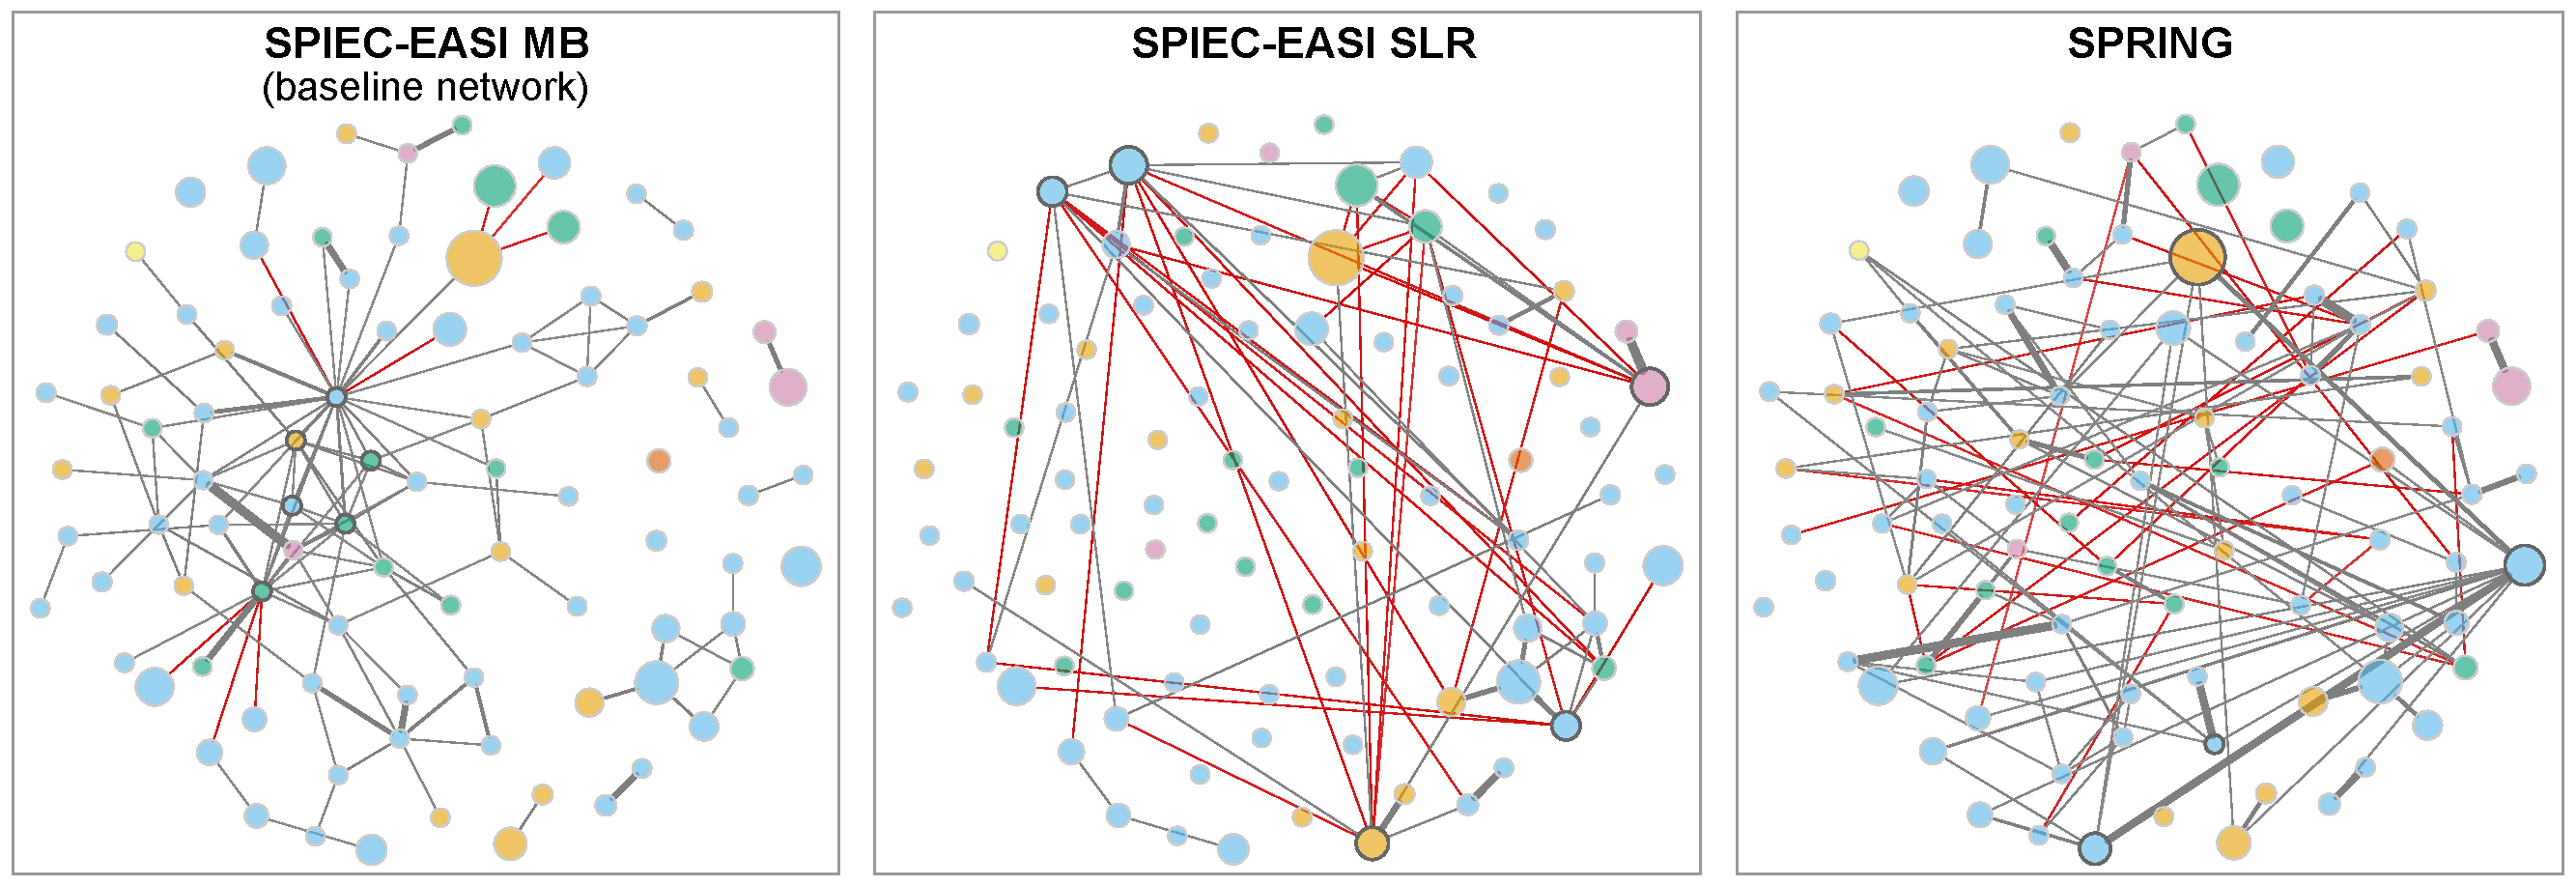
\includegraphics[width=\textwidth]{../ch07_application/figures/10_network_analysis/thesis_combined_networks_association.pdf}
\caption{\textbf{Association networks estimated with alternative conditional-dependence methods.} The left panel shows the SPIEC-EASI MB baseline network. The center and right panels show networks estimated using SPIEC-EASI sparse-plus-low-rank estimation and SPRING, respectively. Node positions, labels, colors, and sizes were kept consistent across panels to facilitate comparison. Nodes represent genera and are colored according to phylum, whereas node sizes are proportional to the mean CLR coordinate across samples. Gray and red edges indicate positive and negative estimated associations, respectively.}
\label{fig:7app:network:combined_association}
\end{figure}

The large number of negative associations estimated by the sparse-plus-low-rank approach also motivates an alternative network representation. In the \emph{signed} network used above, strong negative associations correspond to large dissimilarities and \text{therefore} receive low edge weights. We therefore additionally constructed an unsigned SLR network, as described in Section~\ref{sec:5net:net_construction}. Under this representation, positive and negative associations of large magnitude are both treated as strong connections. Figure~\ref{fig:7app:network:spiecEasi_slr_unsigned_net} shows that several associations involving genera highlighted in the preceding analyses become visually prominent. In particular, \emph{Bacteroides} is strongly positively associated with \emph{Parabacteroides} and strongly negatively associated with \emph{Enterococcus}. The negative associations of \emph{Bifidobacterium} with \emph{Enterobacteriaceae(F)} and \emph{Clostridium sensu stricto 1} are also retained. These patterns should be interpreted as conditional associations estimated under the SLR model rather than as direct biological interactions.

\begin{figure}[!htb]
\centering
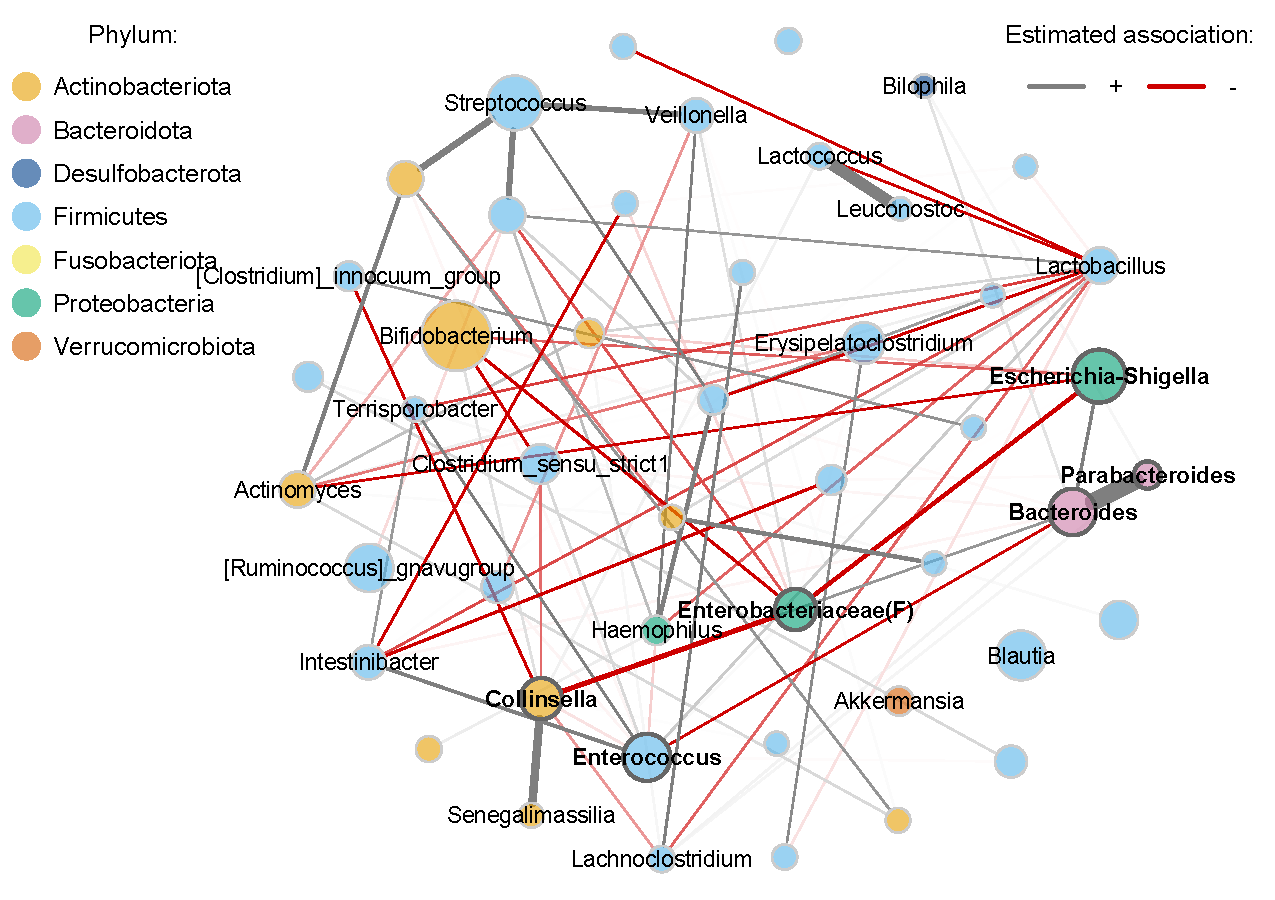
\includegraphics[width=\textwidth]{../ch07_application/figures/10_network_analysis/thesis_single_net_plot_slr_us-1.pdf}
\caption{\textbf{Unsigned network based on SPIEC-EASI SLR estimation.} The network is based on the same sparse-plus-low-rank (SLR) association estimates shown in Figure~\ref{fig:7app:network:combined_association}, but uses the unsigned association-to-similarity transformation. Positive and negative estimated associations with large magnitude therefore both contribute strongly to network connectivity. Nodes represent genera and are colored according to phylum. Node sizes are proportional to the mean CLR coordinate across samples. Gray and red edges indicate positive and negative estimated associations, respectively.}
\label{fig:7app:network:spiecEasi_slr_unsigned_net}
\end{figure}

%------------------------------------
\subsubsection{Persistent edges across sensitivity analyses}
\label{sec:7app:network:sensitivity:persistent_edges}
%------------------------------------

The preceding analyses demonstrated that the estimated network structure changes substantially when prevalence filtering, zero replacement, or association estimation are modified. To summarize the resulting edge-set overlap, UpSet plots were generated separately for the three types of sensitivity analysis.

 Figure~\ref{fig:7app:network:upset_association} shows the comparison across association-estimation methods. The corresponding overlap summaries for prevalence filtering and zero replacement are provided in the thesis repository.
The three association-estimation approaches share only $11$ edges, despite containing between $124$ and $186$ edges in total. This limited overlap reinforces the visual impression that the inferred association structure depends strongly on the selected estimation method. Nevertheless, several taxon pairs occur repeatedly across the different analyses. To identify associations that are comparatively robust to the examined network-construction choices, we considered the $8$ distinct signed networks obtained across all sensitivity analyses: the baseline network, the two networks based on stronger prevalence filters, the three alternative zero-replacement networks, and the two networks based on alternative association-estimation methods.

\begin{figure}[!htb]
\centering
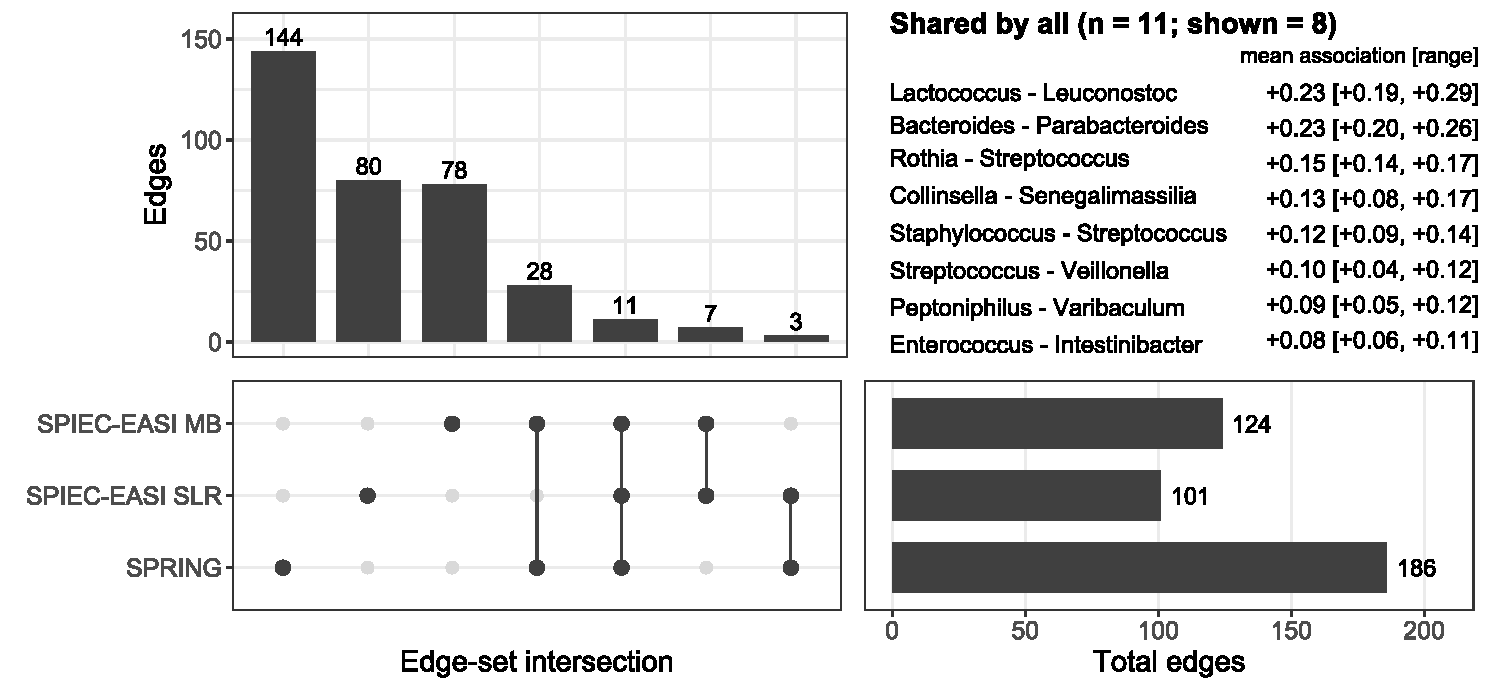
\includegraphics[width=\textwidth]{../ch07_application/figures/10_network_analysis/thesis_edge_upset_association8.pdf}
\caption{\textbf{Shared edges across association estimation methods.} The UpSet plot summarizes overlap among the edge sets estimated by SPIEC-EASI MB, SPIEC-EASI SLR estimation, and SPRING. The upper bar chart shows the number of edges in each intersection, the lower panel indicates the methods contributing to each intersection, and the horizontal bars show the total number of edges in each network. For example, 11 edges are shared among all methods, 3 edges appear only in the SPRING and SLR networks, and 144 only in the SPRING network. The list on the top right shows $8$ of the $11$ edges shared by all three methods, together with their mean estimated association and range across methods.}
\label{fig:7app:network:upset_association}
\end{figure}

Six edges were present in all $8$ networks. Table~\ref{tab:7app:network:persistent_edges} summarizes their estimated association strengths within the three sensitivity-analysis groups and across all selected networks. All six associations are positive, with \emph{Lactococcus}--\emph{Leuconostoc} and \emph{Bacteroides}--\emph{Parabacteroides} showing the largest mean association across the selected networks. The persistence of these edges does not establish their biological origin or imply direct microbial interaction. However, compared with associations that appear only under particular preprocessing or estimation choices, they represent candidate relationships that are less sensitive to the methodological variations considered here.

\begin{table}[!htb]
	\centering
	\caption{\textbf{Edges persistent across sensitivity analyses.} The table lists taxon pairs connected in all eight signed networks considered across prevalence-filtering, zero-replacement, and association-estimation sensitivity analyses. Entries are mean estimated associations within the respective analysis group and across all eight networks.}
	\label{tab:7app:network:persistent_edges}
	\vspace{0.5em}
	\small
	\begin{tabularx}{\textwidth}{l l c c c c}
		\toprule
		Taxon 1 & Taxon 2 & Prevalence filter & Zero repl. & Association & Overall \\
		\midrule
		\emph{Bacteroides} & \emph{Parabacteroides} & $0.20$ & $0.19$ & $0.23$ & $0.208$ \\
		\emph{Rothia} & \emph{Streptococcus} & $0.13$ & $0.13$ & $0.15$ & $0.138$ \\
		\emph{Streptococcus} & \emph{Veillonella} & $0.11$ & $0.11$ & $0.10$ & $0.104$ \\
		\emph{Collinsella} & \emph{Senegalimassilia} & $0.08$ & $0.09$ & $0.13$ & $0.101$ \\
		\emph{Staphylococcus} & \emph{Streptococcus} & $0.08$ & $0.10$ & $0.12$ & $0.100$ \\
		\emph{Gemella} & \emph{Streptococcus} & $0.05$ & $0.05$ & $0.03$ & $0.044$ \\
		\bottomrule
	\end{tabularx}
\end{table}

%%%%%%%%%%%%%%%%%%%%%%%%%%%%%%%%%%%%%
\section{Network comparison between EBF groups}
\label{sec:7app:network}
%%%%%%%%%%%%%%%%%%%%%%%%%%%%%%%%%%%%%

The preceding section examined the sensitivity of a single network estimated from the complete data set to sparsity, zero handling, and association-estimation choices. We now turn to the comparison of association networks estimated separately for children without EBF (``non-EBF'' group) and children with an EBF duration of at least two months (``EBF'' group). This extends the comparative analyses presented in the preceding sections from marginal community- and feature-level differences to differences in estimated association structure. As in the single-network analysis, we revisit genera that were identified as differentially abundant, showed differential distributions, or had high mean CLR coordinates to examine whether they are also involved in differential associations between the two EBF groups. Beyond such taxon- and edge-specific patterns, we investigate whether local or global network characteristics differ significantly between the groups.

The group-specific network analyses were based on the default analysis data set defined in Section~\ref{sec:7app:default_data}, comprising $179$ children in the non-EBF group and $375$ children in the EBF group. As in the preceding network analyses, all networks were estimated at genus level after applying the $1\%$ prevalence filter.

%====================================
\subsection{Descriptive comparison}
\label{sec:7app:network:comparison}
%====================================

Several network-construction approaches were considered. These included SPIEC-EASI MB with Bayesian-multiplicative replacement, SPIEC-EASI sparse-plus-low-rank (SLR) estimation, and SPRING. These three approaches were already considered for the complete data set and yielded networks in which highly sparse genera were less prominently connected than in the baseline SPIEC-EASI MB network based on multiplicative replacement. They are therefore plausible candidates for the subsequent group comparison. For these three methods, the same configuration as in the preceding sections was used. In particular, the regularization path comprised $30$ candidate $\lambda$ values, StARS was based on $30$ subsamples with a stability threshold of $0.1$, and SPIEC-EASI SLR used rank $r=2$, as selected in the analysis of the complete data set.

In addition, correlation shrinkage (cf. Section~\ref{sec:5net:net_constr:sparse_cov_est}) and proportionality shrinkage (cf. Section~\ref{sec:5net:net_constr:prop_shrink}) were considered because shrinkage-based estimators have been reported to be more stable across different sample sizes than several non-shrinkage association estimators \citep{badri2020shrinkage}. Correlation shrinkage was applied to CLR-transformed data, whereas proportionality shrinkage was applied directly to the corresponding zero-replaced compositions. Both approaches were evaluated after either multiplicative replacement (MultRepl) or Bayesian-multiplicative replacement (BayesMultRepl). Because shrinkage estimators generally yield dense association matrices, additional thresholding was used to obtain sparse networks with edge densities comparable to those of the SPIEC-EASI and SPRING networks. Based on the empirical distributions of the estimated associations, an absolute association threshold of $0.3$ was used for networks based on MultRepl and a threshold of $0.15$ for networks based on BayesMultRepl.

Figure~\ref{fig:7app:network:comparison_collection} provides an initial visual comparison of selected group-specific networks. The two SPIEC-EASI approaches and SPRING are displayed in the left panels, and three shrinkage approaches on the right side. Proportionality shrinkage with MultRepl is not shown here, but has a structure similar to that obtained with correlation shrinkage and MultRepl (see also Table~\ref{tab:7app:network:global_measures_comparison}). Labels are omitted because the purpose of this figure is to compare the overall network structures rather than to interpret individual associations. Within each method, the same force-directed layout was used for the two EBF groups. Layouts are the same within one approach, but differ between approaches to preserve the visual network structure within one construction method. In all cases, the repulsion parameter was set to $0.9$ to support broadly comparable visual spacing between nodes.

The overall structure of the SPIEC-EASI SLR and SPRING networks is consistent with the corresponding single-network analyses in the preceding section: both methods yield numerous negative associations, whereas the SLR networks are generally denser than the SPRING networks. In addition, both SPIEC-EASI approaches show a pronounced difference in density between the two EBF groups: the non-EBF networks are substantially denser than the corresponding EBF networks.

Such a pattern can generally arise when networks are constructed from groups of different sample sizes. For a correlation estimator followed by fixed-threshold sparsification, estimates in the smaller group are more variable around their population values, making it more likely that some estimated associations exceed the threshold in absolute value \citep{fisher1921probable}. The present SPIEC-EASI analyses do not use fixed-threshold sparsification, but select the regularization level by StARS. Thus, the preceding argument does not directly imply the observed density difference. Nevertheless, neither SPIEC-EASI nor SPRING can generally be assumed to yield directly comparable network densities when the group sizes differ substantially like in this analysis.

This motivated the additional consideration of correlation and proportionality shrinkage. When used after MultRepl, both shrinkage approaches again produced connected regions dominated by low-abundance genera, indicating that shrinkage alone does not resolve the sensitivity to zero replacement observed in the preceding section. However, the overall connectivity was more similar between the two EBF groups than for the SPIEC-EASI MB networks. We therefore repeated the shrinkage-based analyses using BayesMultRepl. Under both correlation and proportionality shrinkage, the EBF network was then denser than the non-EBF network. Note that these observations are purely descriptive and should not be interpreted as evidence that the shrinkage approaches are generally robust to unequal group sizes, because the true underlying network structures are unknown and no systematic simulation study was conducted in the present analysis.

\begin{figure}[!htb]
\centering
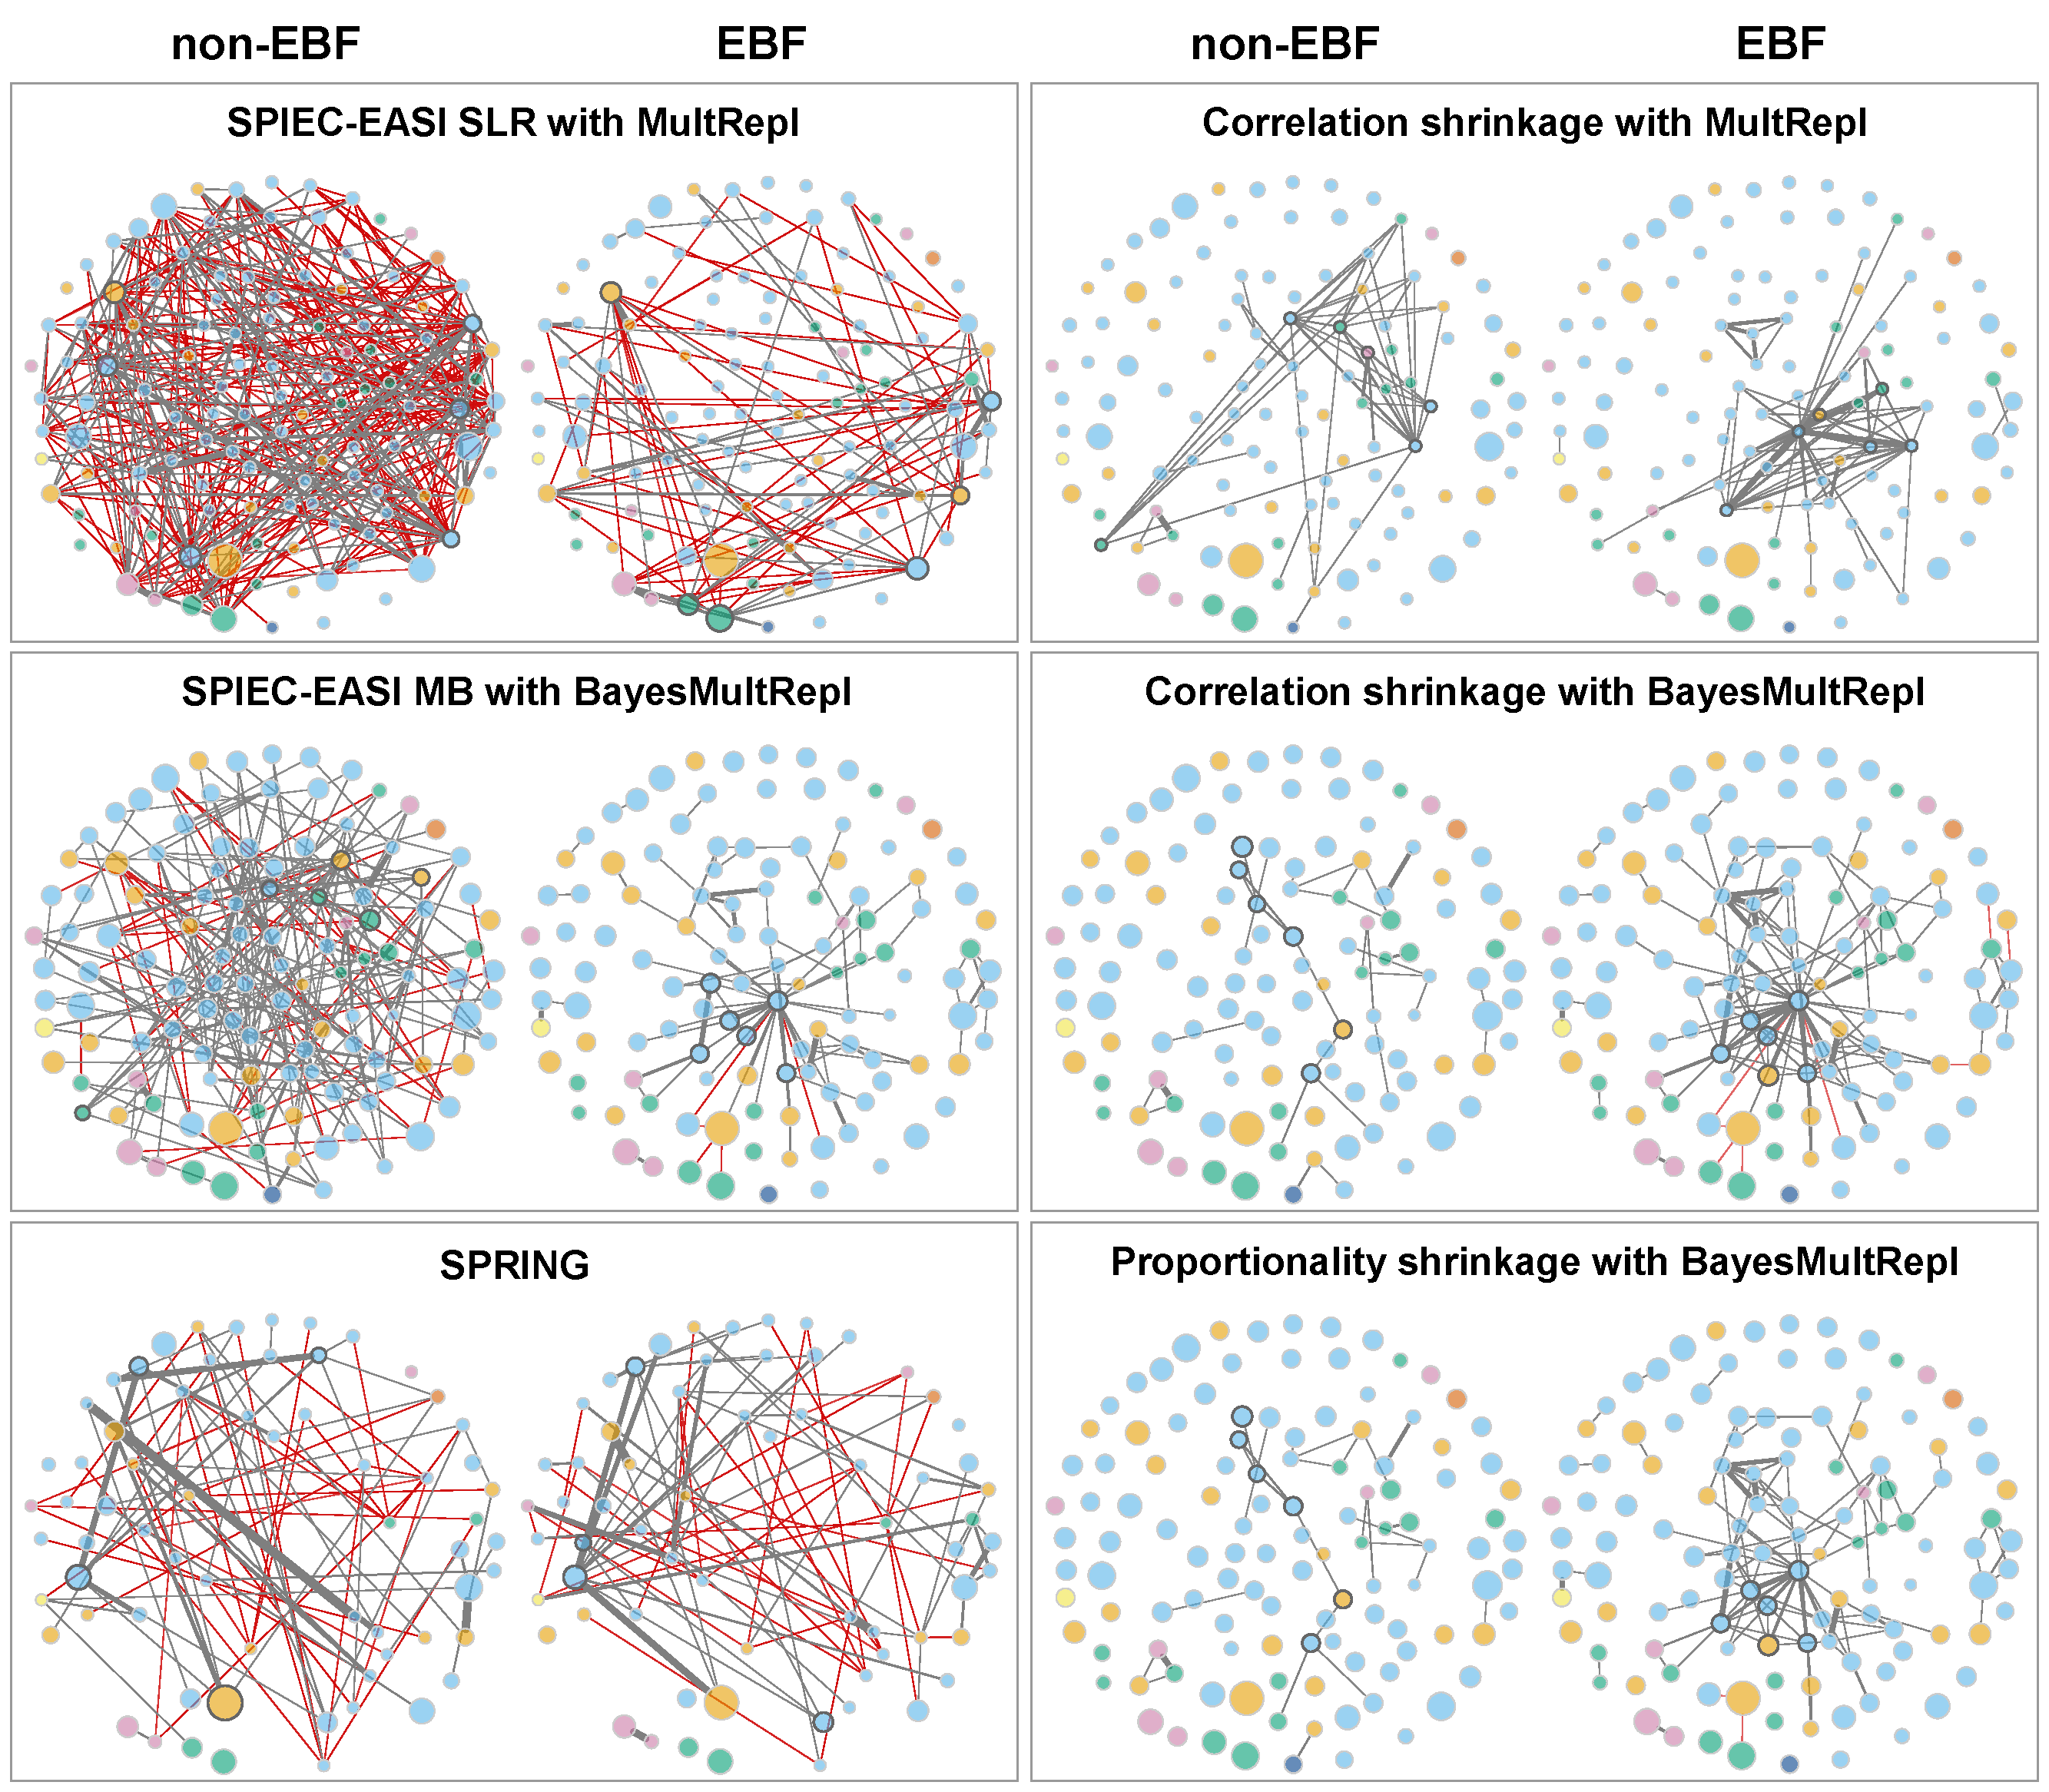
\includegraphics[width=\textwidth]{../ch07_application/figures/11_network_comparison/thesis_combined_networks.pdf}
\caption{\textbf{Group-specific association networks estimated with selected construction approaches.} Networks were estimated separately for non-EBF group ($n=179$) and the EBF group ($n=375$). The displayed approaches are SPIEC-EASI MB with Bayesian-multiplicative replacement (BayesMultRepl), SPIEC-EASI sparse-plus-low-rank (SLR) estimation, SPRING, correlation shrinkage with multiplicative replacement, proportionality shrinkage with BayesMultRepl, and correlation shrinkage with BayesMultRepl. Nodes represent genera and are colored according to phylum, with color coding analogous to Figures~\ref{fig:7app:network:baseline_network} and \ref{fig:7app:network:spiecEasi_slr_unsigned_net}. Node sizes are proportional to the mean CLR coordinate within the respective EBF group. Gray and red edges indicate positive and negative estimated associations, respectively. Labels are omitted to emphasize overall network structure. Within each method, node positions were determined using a common force-directed layout for both EBF groups, with repulsion parameter $0.9$.}
\label{fig:7app:network:comparison_collection}
\end{figure}

Table~\ref{tab:7app:network:global_measures_comparison} summarizes selected global network characteristics for all construction approaches. The relative size of the largest connected component, edge density, and natural connectivity reflect the visual differences in network structure. Across the shrinkage-based approaches, the EBF duration $\geq 2$ group generally has a larger largest connected component (LCC), higher edge density, and greater natural connectivity than the EBF duration $=0$ group. The opposite pattern is observed for the two SPIEC-EASI networks, for which all three network properties are larger in the EBF duration $=0$ group. For SPRING, the corresponding values are broadly similar between groups. These findings mirror the visual impressions from the network plots and demonstrate that apparent group differences in network connectivity depend strongly on the complete network-construction pipeline. Formal comparison of a selected network-construction approach using statistical tests is therefore considered in the following subsection.


\begin{table}[!htb]
\centering
\caption{\textbf{Selected global properties of group-specific association networks.} The table summarizes the relative size of the largest connected component (LCC), edge density, and natural connectivity for networks estimated separately in the two EBF groups. These measures are part of \texttt{NetCoMi}'s analysis summary. Within each method and network property, the larger of the two group-specific values is shown in bold.}
\label{tab:7app:network:global_measures_comparison}
\vspace{0.5em}
\small
\setlength{\tabcolsep}{2.5pt}
\renewcommand{\arraystretch}{1.05}
\begin{tabular}{p{2cm} *{7}{>{\centering\arraybackslash}p{1.7cm}}}
\toprule
& \multicolumn{1}{c}{MB} & \multicolumn{1}{c}{SLR} & \multicolumn{1}{c}{SPRING} & \multicolumn{2}{c}{Cor. shrinkage} & \multicolumn{2}{c}{Prop. shrinkage} \\
\cmidrule(lr){2-2}\cmidrule(lr){3-3}\cmidrule(lr){4-4}\cmidrule(lr){5-6}\cmidrule(lr){7-8}
& BayesMult & MultRepl & -- & MultRepl & BayesMult & MultRepl & BayesMult \\
\midrule
\multicolumn{8}{l}{\textit{Relative LCC size}} \\
non-EBF & $\mathbf{0.983}$ & $\mathbf{0.641}$ & $\mathbf{0.938}$ & $0.145$ & $0.068$ & $0.128$ & $0.068$ \\
EBF & $0.513$ & $0.368$ & $0.892$ & $\mathbf{0.265}$ & $\mathbf{0.650}$ & $\mathbf{0.214}$ & $\mathbf{0.402}$ \\
\addlinespace
\multicolumn{8}{l}{\textit{Edge density}} \\
non-EBF & $\mathbf{0.033}$ & $\mathbf{0.046}$ & $0.041$ & $0.008$ & $0.005$ & $0.006$ & $0.004$ \\
EBF & $0.014$ & $0.015$ & $\mathbf{0.046}$ & $\mathbf{0.012}$ & $\mathbf{0.023}$ & $\mathbf{0.010}$ & $\mathbf{0.017}$ \\
\addlinespace
\multicolumn{8}{l}{\textit{Natural connectivity}} \\
non-EBF & $\mathbf{0.011}$ & $\mathbf{0.013}$ & $0.018$ & $0.010$ & $0.009$ & $0.010$ & $0.009$ \\
EBF & $0.010$ & $0.010$ & $\mathbf{0.019}$ & $\mathbf{0.012}$ & $\mathbf{0.011}$ & $\mathbf{0.012}$ & $\mathbf{0.011}$ \\
\bottomrule
\end{tabular}
\end{table}

%====================================
\subsection{Defining the network construction approach}
\label{sec:7app:network:comparison:approach}
%====================================

The preceding subsection made clear that the visual contrast between the two EBF-group networks can not be seen as a fixed feature of the data, but changes with the network-construction pipeline. Its purpose was therefore not to interpret these plots as evidence of differential network structure, but to identify a construction approach that remains reasonably comparable despite the markedly unequal group sizes. We first motivate the selected association measure and preprocessing strategy for the permutation procedure. Building on this choice, the following sections examine whether the two EBF groups differ in global network structure, node-level properties, or individual associations.

Based on the former comparison, correlation shrinkage with Bayesian-multiplicative replacement was selected for the formal analyses. The shrinkage-based networks showed less pronounced differences in overall connectivity between the two EBF groups than the SPIEC-EASI networks, and Bayesian-multiplicative replacement avoided the highly connected subnetworks of low-abundance genera observed when correlation or proportionality shrinkage was combined with multiplicative replacement. Correlation shrinkage was preferred over proportionality shrinkage because the estimated correlations can additionally be compared between groups using Fisher's $z$-test. This provides an edge-wise complement to the permutation-based approach for differential association analysis.

SPRING was also considered a suitable candidate because its modified CLR transformation avoids external zero replacement. However, network construction could not be completed successfully for a substantial number of permuted group allocations, even after considerably stricter prevalence filtering. In these cases, the fitted model returned missing association estimates. A permutation analysis would then require a principled treatment of failed model fits in the null distribution, including a definition of the test statistic when one or both group-specific networks cannot be estimated. This methodological issue is beyond the scope of the present application.

The SPIEC-EASI MB and SLR approaches were not selected because both produced substantially denser networks for the smaller EBF duration $=0$ group. Although unequal densities do not preclude a formal network comparison, they complicate the interpretation of differences in global and local network properties when the groups differ markedly in sample size. For the SLR approach, this concern was accompanied by a comparatively large number of negative estimated associations. We therefore did not pursue these methods for the formal comparison.

A further decision concerned the role of Bayesian-multiplicative replacement in the permutation procedure. This replacement method estimates prior parameters from the samples included in the data set to which it is applied. Repeating replacement separately within each permuted group would therefore change the group-specific priors and the resulting replacement values after every relabeling. In that formulation, zero replacement forms part of the group-specific network-construction procedure and must be repeated for each permutation.

In the present data set, however, separate Bayesian-multiplicative replacement failed for some permuted group allocations because of the extreme sparsity of the count matrix. We therefore applied Bayesian-multiplicative replacement once to the complete, globally filtered data set before splitting the samples into the observed or permuted EBF groups. The resulting positive composition matrix was treated as a fixed sample representation throughout the permutation procedure, whereas correlation estimation, network construction, and calculation of the respective comparison statistics were repeated after each permutation.

This defines the target of inference as differences between networks estimated from a common Bayesian-multiplicative representation of all samples, rather than differences after separately estimated group-specific replacement models. This choice is coherent because the two EBF groups are subsets of the same cohort and are measured on a common feature table, rather than representing separate sequencing experiments with potentially distinct detection limits. Joint preprocessing also avoids introducing differences in the estimated replacement prior solely through the permutation of group labels.

%====================================
\subsection{Permutation procedure}
\label{sec:7app:network:comparison:permutation}
%====================================

Permutation testing was implemented using the \texttt{createAssoPerm()} function in \texttt{NetCoMi}. This function generates association matrices for permuted group allocations and stores them for subsequent reuse. The resulting matrices can be supplied to \texttt{netCompare()} for testing differences in global and node-level network properties and to \texttt{diffnet()} for testing differential associations. Storing the permuted association matrices ensures that all downstream tests are based on the same set of permuted group allocations and avoids repeated association estimation for each individual comparison statistic.

A further practical advantage of this workflow is that the association matrices can be generated in separate blocks of permutations. This was necessary in the present analysis because generating and storing all permuted matrices simultaneously exceeded the available memory capacity. We therefore performed the permutation procedure in blocks of $20$ permutations. These blocks were computed in parallel, and a separate seed was used for each repetition to ensure reproducibility of the complete permutation procedure. A total of $999$ permutations was generated, consistent with the permutation analyses in the preceding application sections.

The stored permutation matrices were subsequently reused by \texttt{netCompare()} to test differences in global and node-level network properties. As described in Chapter~\ref{ch:netcomi}, we refer to this analysis as ``differential network analysis''. For each test statistic, three $p$-values were considered: the empirical permutation $p$-value, the unconstrained \texttt{permApprox}-refined $p$-value, and the constrained \texttt{permApprox}-refined $p$-value. The results are presented in the following subsection.

The same permutation matrices were then used in \texttt{diffnet()} to test individual differential associations between the EBF groups. In accordance with the terminology introduced in Chapter~\ref{ch:netcomi}, this edge-wise analysis is referred to as ``differential association analysis''. The approach was the same as for the differential network analysis, with the exception that we did not use the default \texttt{permApprox} configuration here, because it led to overly conservative $p$-values compared to the unconstrained ones. We therefore changed the approach to use the maximum of the observed test statistics instead of the permuted ones as saturation cap. In addition we set the tuning parameter to 0.1. The results are presented in Section~\ref{sec:7app:network:comparison:associations}.

The same permutation matrices were then used in \texttt{diffnet()} to test individual differential associations between the EBF groups. In accordance with the terminology introduced in Chapter~\ref{ch:netcomi}, this edge-wise analysis is referred to as ``differential association analysis.'' The analysis followed the same $p$-value refinement strategy as the differential network analysis, but used a modified \texttt{permApprox} configuration. Under the default settings, the constrained \texttt{permApprox} $p$-values were substantially larger than the corresponding unconstrained estimates. We therefore changed the saturation cap to use the maximum of the observed edge-wise test statistics rather than the maximum of the permuted test statistics, and set the tuning parameter to $0.1$. The results are presented in Section~\ref{sec:7app:network:comparison:associations}.

%====================================
\subsection{Differential network analysis}
\label{sec:7app:network:comparison:global}
%====================================

Figure~\ref{fig:7app:network:ebf_network} shows the group-specific correlation-shrinkage networks estimated after Bayesian-multiplicative replacement. A common force-directed layout was used for both networks so that differences in the displayed association structure can be assessed without being confounded by changes in node positions. Like already observed in the descriptive comparison, both networks are sparse and contain several disconnected components. In addition to the general difference in edge density, their local structures also differ visibly in several regions. Most notably, \emph{Coprobacillus} is disconnected in the EBF duration $=0$ network, whereas it is highly connected (to 32 other genera) in the EBF network. These differences in connectivity are also reflected in the degree distributions shown in Figure~\ref{fig:7app:network:ebf_degree_distribution}. The CLR-coordinate heatmap in Figure~\ref{fig:app:7app:net_compare_clr_heatmap} shows that the mean CLR coordinates after Bayesian-multiplicative replacement of \emph{Coprobacillus} are not high compared to other genera but it is also not among the rarest ones. Nevertheless, the possibility that the high connectivity in the EBF network is an artifact of zero handling cannot be dismissed.

\begin{figure}[H]
\centering
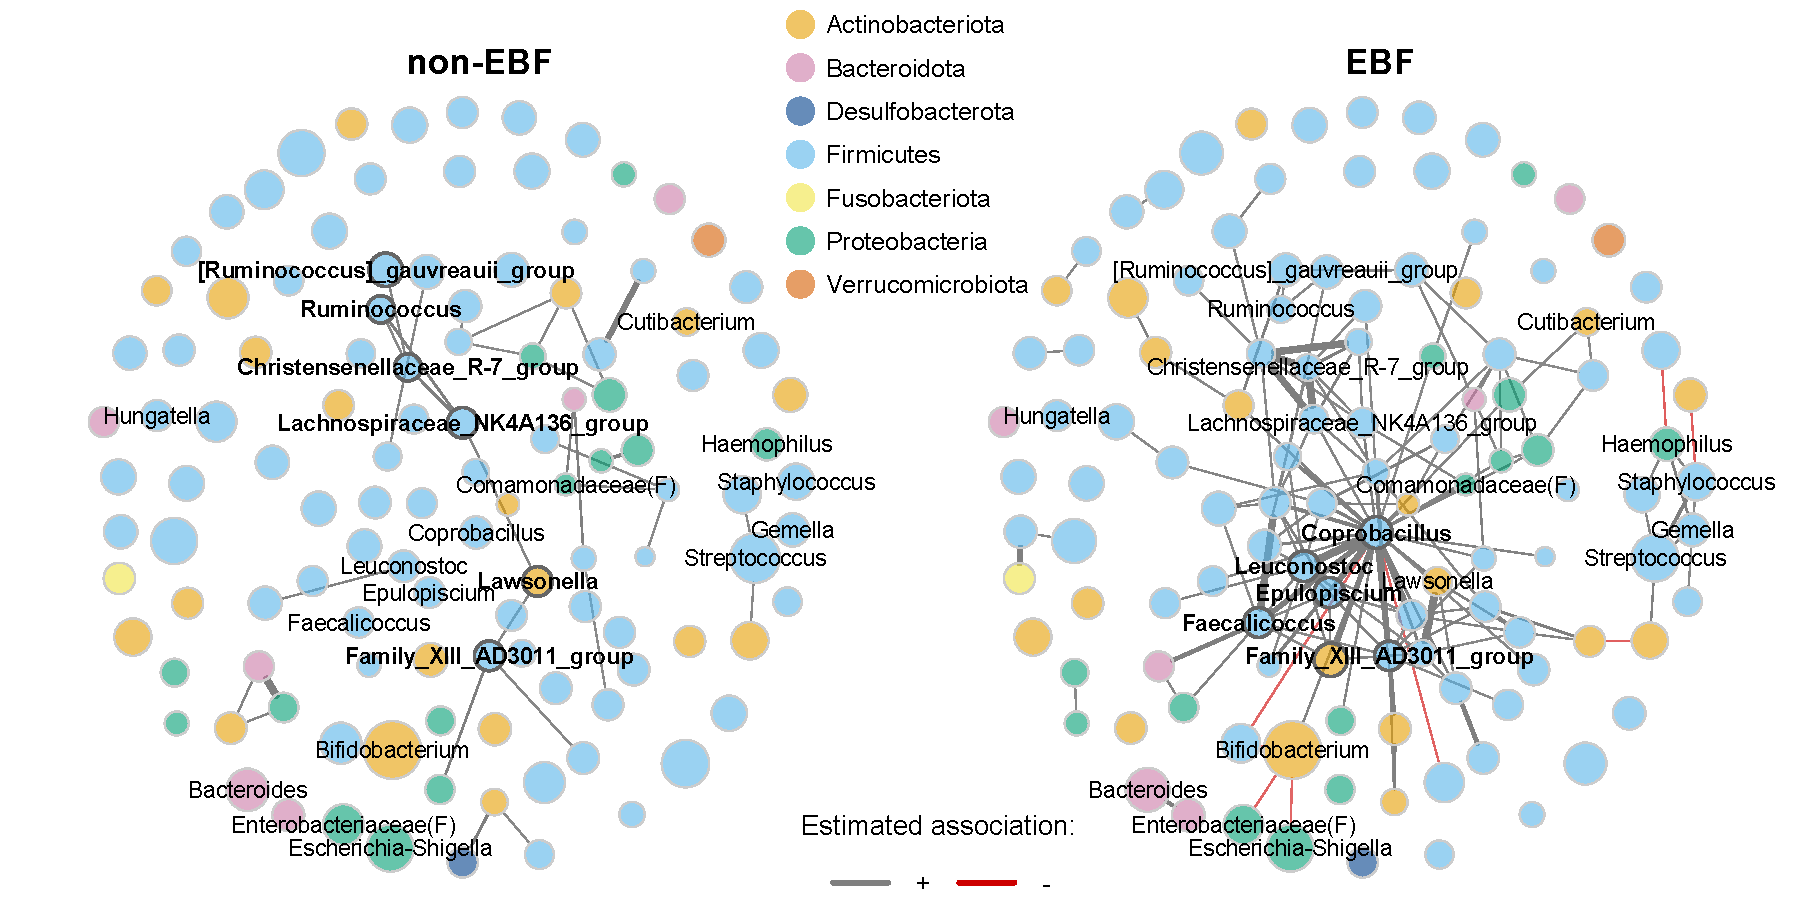
\includegraphics[width=\textwidth]{../ch07_application/figures/11_network_comparison/thesis_ebf_network_plot_same_layout-1.pdf}
\caption{\textbf{Group-specific correlation shrinkage networks.} Networks were estimated separately for the non-EBF and the EBF group, using the approach described in Section~\ref{sec:7app:network:comparison:approach}. Nodes represent genera and are colored according to phylum. Node sizes are proportional to the mean CLR coordinate within the respective EBF group. Gray and red edges indicate positive and negative estimated correlations, respectively. A common force-directed layout was used for both networks to facilitate visual comparison of their association structures. Labels identify genera considered in the preceding differential abundance and differential distribution analyses, together with selected genera highlighted in the network comparison.}
\label{fig:7app:network:ebf_network}
\end{figure}

\begin{figure}[H]
\centering
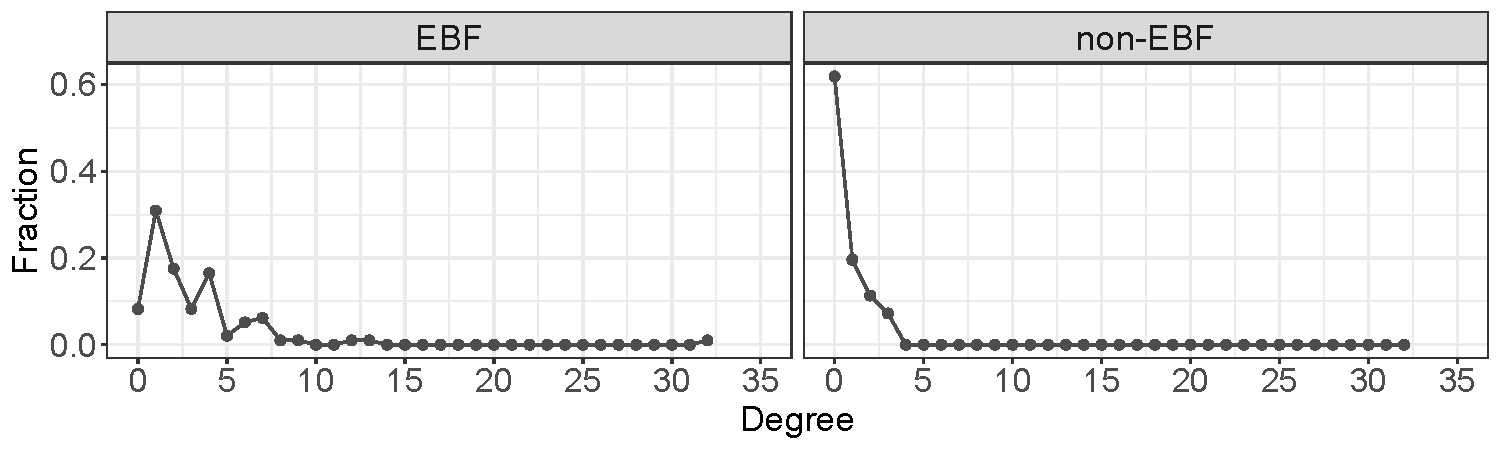
\includegraphics[width=0.9\textwidth]{../ch07_application/figures/11_network_comparison/thesis_ebf_degree_distribution_side_by_side-1.pdf}
\caption{\textbf{Degree distributions of the two EBF networks.} The panels show the distributions of non-normalized node degree for the correlation-shrinkage networks estimated separately for the EBF and non-EBF group. Nodes with degree zero correspond to disconnected genera.}
\label{fig:7app:network:ebf_degree_distribution}
\end{figure}

The \texttt{netCompare()} output, parts of which are shown below, provides further insight into whether the visual differences are reflected in numerical differences between network measures and whether these differences are larger than expected under permutation of the EBF-group labels. For each measure, the output below reports the values in the two groups, their absolute difference, and the empirical permutation $p$-value. No multiple-testing adjustment was applied because the global network properties were interpreted as distinct summary measures rather than as a common family of hypotheses. Refining the $p$-values with \texttt{permApprox} had no effect because all empirical $p$-values exceeded the threshold below which $p$-values were selected for refinement. The upper part of the output contains measures computed for the largest connected component (LCC), whereas the lower part contains measures that are also meaningful for the complete network. None of the tested differences was statistically significant.


\begin{Verbatim}[fontsize=\footnotesize]
Global network properties
`````````````````````````
Largest connected component (LCC):
                         non-EBF    EBF    abs.diff.     $p$-value  
Relative LCC size          0.068  0.650        0.581    0.347000  
Clustering coefficient     0.336  0.440        0.105    0.623000  
Modularity                 0.369  0.535        0.166    0.353000  
Positive edge percentage 100.000 94.558        5.442    0.377000  
Edge density               0.286  0.052        0.234    0.210000  
Natural connectivity       0.192  0.019        0.173    0.133000  
Vertex connectivity        1.000  1.000        0.000    1.000000  
Edge connectivity          1.000  1.000        0.000    1.000000  
Average dissimilarity*     0.895  0.981        0.086    0.207000  
Average path length**      1.744  2.458        0.715    0.361000  

Whole network:
                         non-EBF    EBF    abs.diff.     $p$-value  
Number of components      90.000 35.000       55.000    0.262000  
Clustering coefficient     0.408  0.433        0.025    0.908000  
Modularity                 0.840  0.565        0.275    0.443000  
Positive edge percentage 100.000 94.805        5.195    0.259000  
Edge density               0.005  0.023        0.018    0.461000  
Natural connectivity       0.009  0.011        0.002    0.543000  
-----
$p$-values: one-tailed test with null hypothesis diff=0
 *: Dissimilarity = 1 - edge weight
**: Path length = Units with average dissimilarity
\end{Verbatim}

The following output shows the graphlet correlation distances (GCD) in the two groups, which provides a complementary comparison of the local topological organization of the networks. In contrast to the preceding global summary measures, it quantifies the overall discrepancy between the graphlet correlation matrices (GCMs) of the two networks. Appendix Figure~\ref{fig:app:7app:net_compare_gcm} shows the corresponding GCM heatmaps, including significance codes resulting from Fisher's z tests.

\begin{Verbatim}[fontsize=\footnotesize]
Graphlet Correlation Distance
`````````````````````````````
        wholeNet         LCC  
GCD        2.372       4.221  
$p$-value 0.161000    0.300000  
-----
GCD >= 0 (GCD=0 indicates perfect agreement between GCMs)
$p$-value: permutation test with null hypothesis GCD=0
\end{Verbatim}

The estimated GCD was $2.372$ for the complete networks and $4.221$ for their largest connected components. Neither value was statistically significant under permutation of the EBF-group labels. Thus, although Fisher's $z$-tests indicated differences for several individual GCM entries, the aggregate difference in graphlet correlation structure was not larger than expected under the permutation null distribution. 

The node-level comparison similarly revealed several descriptive contrasts, particularly for genera that were disconnected in one network but embedded in a connected component in the other. The \texttt{netCompare()} output below lists the centrality measures with the smallest unadjusted permutation $p$-values. The output shows for genus the centrality values in the two groups, their absolute difference, as well as the empirical $p$-values before and after adjustment for multiplicity. The \texttt{permApprox}-refined $p$-values were almost identical to the empirical $p$-values because none of the $p$-values was below the minimum attainable empirical $p$-value for $999$ permutations. Consequently, $p$-value refinement did not affect any inferential decision.

\begin{Verbatim}[fontsize=\footnotesize]
Centrality measures
- In increasing order of unadjusted $p$-values
````````````````````````````````````````````````
Degree (unnormalized):
               non-EBF EBF abs.diff.  $p$-value     adj.$p$-value  
Leuconostoc          0  13        13 0.016000 *      1.000000  
Lactobacillus        0   1         1 0.042000 *      1.000000  
Staphylococcus       0   4         4 0.043000 *      1.000000  
Coprobacillus        0  32        32 0.048000 *      1.000000  
Gemella              0   4         4 0.080000 .      1.000000  

Betweenness centrality (unnormalized):
              non-EBF  EBF abs.diff.  $p$-value     adj.$p$-value  
Rothia              0  536       536 0.002000 **     0.156000  
Varibaculum         0  594       594 0.003000 **     0.156000  
Coprobacillus       0 1936      1936 0.004000 **     0.156000  
Peptoniphilus       0  610       610 0.007000 **     0.204750  
Streptococcus       0  478       478 0.015000 *      0.351000  

Closeness centrality (unnormalized):
              non-EBF    EBF abs.diff.  $p$-value     adj.$p$-value  
Lactobacillus       0 16.938    16.938 0.042000 *      0.715565  
Leuconostoc         0 59.065    59.065 0.083000 .      0.715565  
Coprobacillus       0 76.861    76.861 0.095000 .      0.715565  
Eggerthella         0 18.573    18.573 0.136000        0.715565  
Epulopiscium        0 53.335    53.335 0.144000        0.715565  

Eigenvector centrality (unnormalized):
                 non-EBF   EBF abs.diff.  $p$-value     adj.$p$-value  
Ruminococcus       0.821 0.007     0.814 0.020000 *      0.959400  
Leuconostoc        0.000 0.639     0.639 0.035000 *      0.959400  
Terrisporobacter   0.000 0.033     0.033 0.037000 *      0.959400  
Coprobacillus      0.000 1.000     1.000 0.037000 *      0.959400  
Lactobacillus      0.000 0.000     0.000 0.041000 *      0.959400  
_________________________________________________________
Significance codes: ***: 0.001, **: 0.01, *: 0.05, .: 0.1
\end{Verbatim}

Before multiplicity adjustment, \emph{Leuconostoc}, \emph{Lactobacillus}, \emph{Staphylococcus}, and \emph{Coprobacillus} showed differences in unnormalized degree, with all four genera having degree zero in the non-EBF network and positive degree in the EBF network. In particular, \emph{Coprobacillus} had degree $32$ in the latter network, consistent with its visually prominent local position in Figure~\ref{fig:7app:network:ebf_network}. Several genera, including \emph{Rothia}, \emph{Varibaculum}, \emph{Coprobacillus}, and \emph{Peptoniphilus}, also had comparatively small unadjusted $p$-values for betweenness centrality.

However, none of the node-level differences remained statistically significant after Benjamini--Hochberg adjustment across genera. The observed centrality contrasts should therefore be interpreted as descriptive patterns rather than as confirmed differential node properties. 

Taken together, the differential network analysis does not provide evidence for global or node-level differences that are robust to the multiplicity adjustment applied here, despite the visible differences between the two estimated networks.

%====================================
\subsection{Differential association analysis}
\label{sec:7app:network:comparison:associations}
%====================================

After comparing the two EBF-group networks at the level of overall network properties, we next examined whether individual associations differed between the groups. This edge-wise analysis was based on the same correlation-shrinkage approach after Bayesian-multiplicative replacement that was used for the differential network analysis. For each of the $\binom{117}{2}=6786$ possible genus pairs, the difference between the two group-specific association estimates was tested by permutation using the precomputed permuted association matrices. Thus, in contrast to an analysis restricted to edges that are non-zero in at least one of the observed networks, the present analysis follows the stricter approach of testing all possible edges in parallel. This leads to a particularly severe multiplicity burden after Benjamini--Hochberg adjustment, but avoids conditioning the tested hypotheses on the observed sparsified networks.

Figure~\ref{fig:7app:network:diffassoc_pvalues} compares the raw empirical permutation $p$-values with the corresponding \texttt{permApprox}-refined $p$-values. The y-axis shows the unadjusted $p$-values, whereas colored points indicate edges that were significant after Benjamini--Hochberg adjustment. As expected from $999$ permutations, the empirical $p$-values are bounded below by $1/(999+1)=0.001$, so the empirical analysis cannot distinguish among the strongest signals. In contrast, the \texttt{permApprox} refinement yields a much more informative ranking of small $p$-values. The unconstrained approximation produced one $p$-value equal to zero, whereas the constrained approximation avoided this artifact and returned finite tail $p$-values throughout. In this example, the unconstrained and constrained results are very similar for most edges, and the constrained approach is only slightly more conservative. In the plot, edges for which the constrained and unconstrained $p$-values were nearly identical are highlighted in yellow, whereas other colors mark edges whose refined $p$-values changed more visibly under the constraint.

\begin{figure}[!htb]
\centering
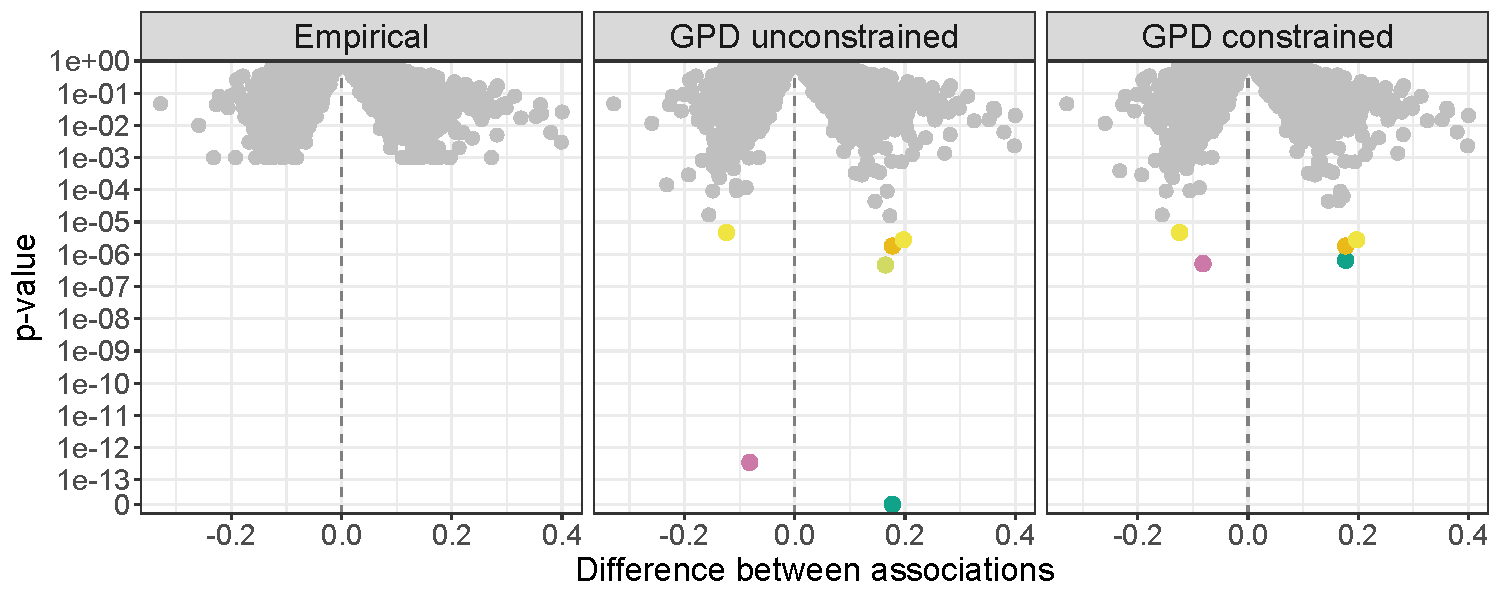
\includegraphics[width=\textwidth]{../ch07_application/figures/11_network_comparison/thesis_diffnet_raw_pvalue_comparison-1.pdf}
\caption{\textbf{Comparison of empirical and \texttt{permApprox}-refined $p$-values for differential associations.} Each point represents one tested genus pair. The y-axis shows the unadjusted $p$-value, and point colors indicate whether the edge was significant after Benjamini--Hochberg adjustment at $\alpha = 5\%$. Because the empirical permutation analysis is based on $999$ permutations, empirical $p$-values are bounded below by $0.001$. The \texttt{permApprox} refinement yields continuous tail $p$-values below this bound. Yellow points indicate genus pairs for which the unconstrained and constrained \texttt{permApprox} $p$-values were nearly identical, whereas other colors highlight more noticeable differences between the two approximations.}
\label{fig:7app:network:diffassoc_pvalues}
\end{figure}


Table~\ref{tab:7app:network:diffassoc_pvalues} lists the raw $p$-values for the edges with the smallest unconstrained \texttt{permApprox} $p$-values. The strongest signals are concentrated in a small set of genera. In particular, several edges involve the cluster around \emph{Streptococcus}, \emph{Staphylococcus}, \emph{Gemella}, and \emph{Haemophilus}, which already stood out in the group-specific network plots. The association between \emph{Gemella} and \emph{Streptococcus} is the most extreme example: its empirical $p$-value is again limited to $0.001$, whereas the unconstrained approximation yields a $p$-value of zero and the constrained approximation still gives a very small but finite value. Other prominent edges include \emph{Hungatella}--\emph{Cutibacterium}, \emph{Scardovia}--\emph{Cutibacterium}, and \emph{[Eubacterium] coprostanoligenes group}--\emph{Lactococcus}.

\begin{table}[!htb]
\centering
\caption{\textbf{Raw $p$-values for selected differential associations.} The table lists the genus pairs with the smallest unconstrained \texttt{permApprox} $p$-values in the differential association analysis, ordered by increasing unconstrained $p$-value. $p_{\mathrm{empirical}}$ denotes the empirical permutation $p$-value, whereas $p_{\mathrm{permApprox(U)}}$ and $p_{\mathrm{permApprox(C)}}$ denote the unconstrained and constrained GPD-based \texttt{permApprox} $p$-values, respectively.}
\label{tab:7app:network:diffassoc_pvalues}
\vspace{0.5em}
\small
\setlength{\tabcolsep}{4pt}
\begin{tabular}{llrrrr}
\toprule
Taxon 1 & Taxon 2 & Difference & $p_{\mathrm{empirical}}$ & $p_{\mathrm{permApprox(U)}}$ & $p_{\mathrm{permApprox(C)}}$ \\
\midrule
\emph{Gemella} & \emph{Streptococcus} & 0.17736534 & 1.00e-03 & 0.00e+00 & 6.50e-07 \\
\emph{Hungatella} & \emph{Cutibacterium} & -0.08159082 & 1.00e-03 & 3.45e-13 & 5.12e-07 \\
\emph{Haemophilus} & \emph{Staphylococcus} & 0.16479100 & 1.00e-03 & 4.63e-07 & 4.53e-05 \\
\emph{Haemophilus} & \emph{Streptococcus} & 0.17737423 & 1.00e-03 & 1.80e-06 & 1.80e-06 \\
\emph{Haemophilus} & \emph{Gemella} & 0.19718139 & 1.00e-03 & 2.80e-06 & 2.80e-06 \\
\emph{Leuconostoc} & \emph{Staphylococcus} & -0.12385940 & 1.00e-03 & 4.73e-06 & 4.73e-06 \\
\emph{Staphylococcus} & \emph{Streptococcus} & 0.17278499 & 1.00e-03 & 1.56e-05 & 6.35e-05 \\
\emph{Scardovia} & \emph{Cutibacterium} & -0.15588102 & 1.00e-03 & 1.67e-05 & 1.67e-05 \\
\emph{[Eubacterium] copro.} & \emph{Lactococcus} & 0.14566499 & 1.00e-03 & 4.40e-05 & 4.40e-05 \\
\bottomrule
\vspace{1em}
\end{tabular}
\end{table}

Figure~\ref{fig:7app:network:diffassoc_network} displays the differential association network, which contains edges with significant between-group differences in association. The network uses the same layout as the two group-specific network plots to facilitate comparison. A striking feature is again the \emph{Streptococcus}-centered region on the right-hand side, where several significant differential associations occur among \emph{Streptococcus}, \emph{Staphylococcus}, \emph{Gemella}, and \emph{Haemophilus}. In contrast, several associations that were visually noticeable in the descriptive network plots, such as the negative associations involving \emph{Bifidobacterium}, were not significant in the formal edge-wise comparison. Some significant edges in the differential association network are not visible in the group-specific network plots because the latter were based on sparsified networks, whereas the differential association analysis uses the underlying raw association estimates before thresholding. Thus, the differential association network highlights changes in association strength between the groups even when the individual associations are too weak to appear as edges in the displayed group-specific networks.

\begin{figure}[!htb]
\centering
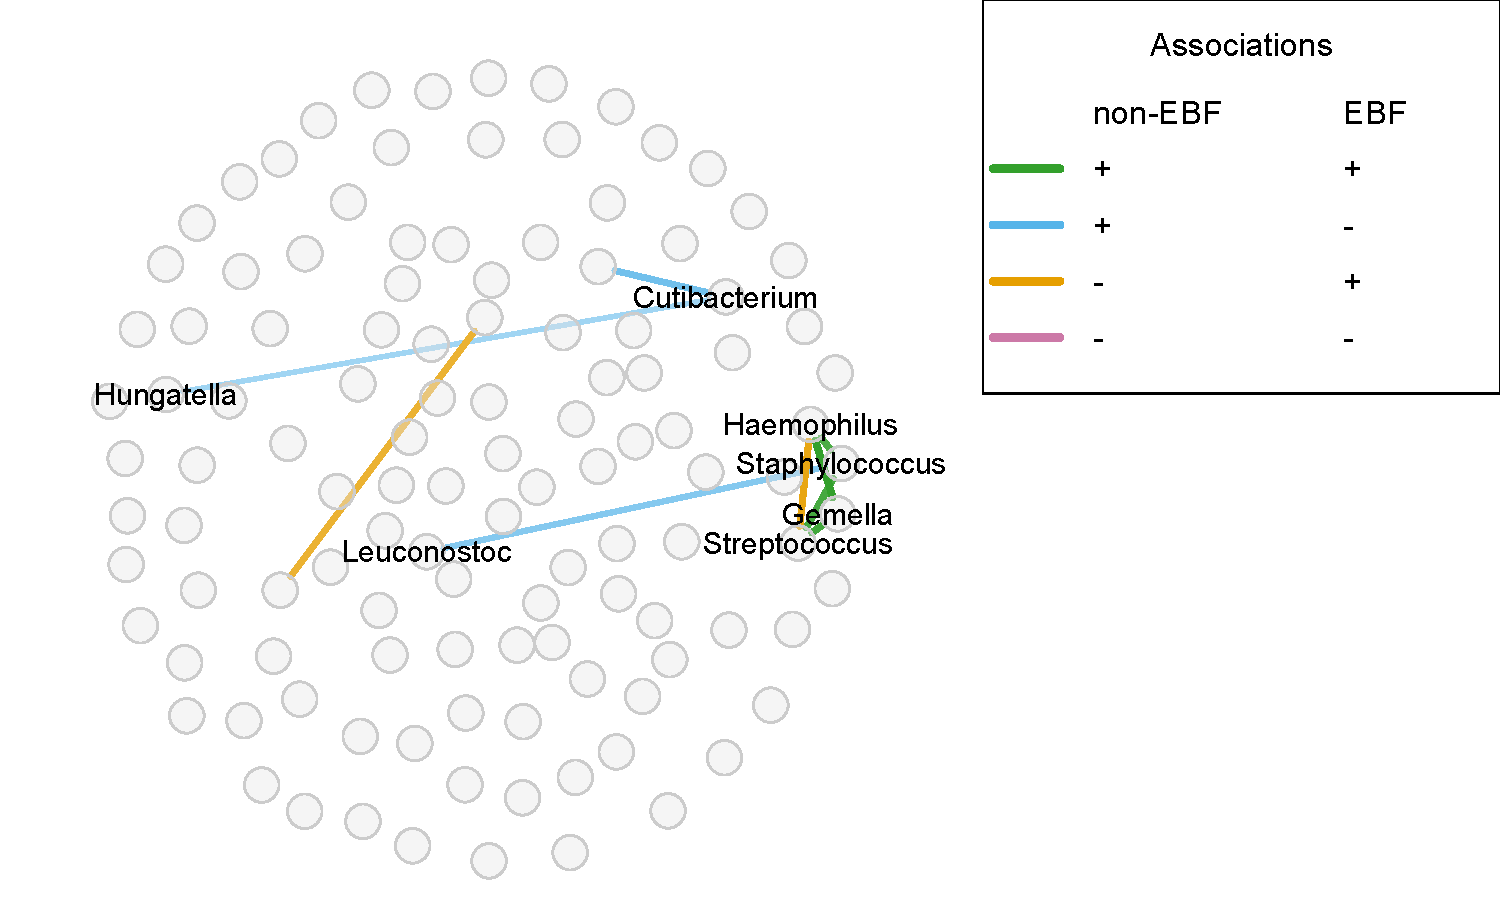
\includegraphics[width=0.9\textwidth]{../ch07_application/figures/11_network_comparison/thesis_ebf_diffnet_plot_same_layout-1.pdf}
\caption{\textbf{Differential association network between the two EBF groups.} Edges represent genus pairs with significant differences in association between children without EBF and children with EBF duration $\geq 2$ months. Edge colors indicate the direction of the association in the two groups. The network uses the same layout as the group-specific network plots to facilitate comparison. Several significant differential associations are concentrated in the \emph{Streptococcus}-centered region, whereas other visually striking associations from the descriptive network plots, such as negative associations involving \emph{Bifidobacterium}, were not significant.}
\label{fig:7app:network:diffassoc_network}
\end{figure}

%%%%%%%%%%%%%%%%%%%%%%%%%%%%%%%%%%%%%
\section{Discussion}
\label{sec:7app}
%%%%%%%%%%%%%%%%%%%%%%%%%%%%%%%%%%%%%

This chapter applied the methodological components developed throughout the thesis to a reduced subset of the PASTURE cohort. The analysis combined community-level summaries, feature-level comparisons, and association-network analyses, using a common genus-level representation where possible while allowing method-specific preprocessing when required. Its primary purpose was to illustrate how these complementary perspectives can be combined in a coherent microbiome workflow, rather than to provide definitive biological conclusions about the effects of breastfeeding in the full PASTURE cohort.

Across the community-level analyses, breastfeeding-related variables emerged as the most consistent sources of variation in the two-month gut microbiome. BF duration and EBF duration were associated with within-sample diversity, between-sample dissimilarity, and mean CLR composition. The analyses also illustrate that these perspectives are related but not interchangeable. The ordination plots did not show clearly separated EBF groups, whereas PERMANOVA, regression-based analyses, and compositional equivalence nevertheless indicated systematic differences when the full multivariate information was used. Thus, the EBF contrast is better interpreted as a gradual shift in community composition than as a division into two distinct microbiome states.

The results further demonstrate the value of distinguishing marginal feature-level effects from broader distributional changes. Differential abundance analysis identified several genera whose relative abundances differed between the EBF groups. \emph{Enterococcus}, \emph{Lactococcus}, \emph{Intestinibacter}, and the \emph{[Ruminococcus] gnavus group} showed higher abundance in children without EBF, whereas \emph{Bifidobacterium} was more abundant in children with EBF duration of at least two months. The latter pattern is consistent with the well-established association between breastfeeding and \emph{Bifidobacterium}-dominated infant gut communities \citep{backhed2015dynamics,stewart2018temporal}.

Differential distribution analysis recovered a partly overlapping set of genera, but additionally distinguished between changes in the distribution among non-zero observations and changes in zero prevalence. This distinction is particularly relevant for sparse microbiome data, where a taxon can differ between groups because of shifts in its positive abundance distribution, because of changes in detection frequency, or through both mechanisms. The agreement between the different feature-level analyses therefore strengthens the interpretation that EBF duration is associated with broad changes in the early gut microbiome, while their differences underline that no single taxon-level method captures all relevant aspects of the data.

The network analyses added a relational perspective to these findings, but also offered strong indications of the sensitivity of microbial network inference to methodological choices. In the complete data set, the apparent prominence of low-abundance genera depended strongly on prevalence filtering, zero replacement, and association estimation. Several edges remained visible across alternative specifications, but the overall network structure and the presence of highly connected taxa changed substantially. This result is not a defect of a particular method; rather, it reflects the limited information available for estimating associations involving sparse taxa. It reinforces the need to interpret microbial association networks as model-dependent summaries of statistical dependence, not as direct reconstructions of ecological interactions.

For the EBF comparison, the selected correlation-shrinkage approach with Bayesian-multiplicative replacement produced group-specific networks that were sufficiently comparable for the subsequent permutation analyses. No robust differences in global network properties or node-level centrality measures were detected after the respective inferential procedures. In contrast, the edge-wise differential association analysis identified several associations that differed between the EBF groups, particularly in the region involving \emph{Streptococcus}, \emph{Staphylococcus}, \emph{Gemella}, and \emph{Haemophilus}. This contrast between largely non-significant global network summaries and significant individual differential associations is not inherently contradictory, because the two analyses target different aspects of network structure and are subject to different multiplicity burdens. The results indicate that the detectable EBF-related differences in the present analysis are concentrated in a limited set of associations, particularly around \emph{Streptococcus}, \emph{Staphylococcus}, \emph{Gemella}, and \emph{Haemophilus}, rather than providing clear evidence for a difference in the selected global network properties. This does not rule out more diffuse structural differences that were not captured by the considered summaries or could not be detected with the available sample sizes and permutation budget.

Permutation-based inference and $p$-value refinement played different roles across the analyses. For tests with moderate $p$-values, empirical permutation inference was adequate and \texttt{permApprox} did not alter the resulting conclusions. Its practical value became most visible when the empirical $p$-value resolution was limiting. In the differential abundance analysis, refinement based on a comparatively small permutation budget yielded a ranking of strong signals that was broadly coherent with a substantially more expensive analysis using $10^7$ permutations. In the differential distribution and differential association analyses, constrained tail approximation avoided zero $p$-values and provided finite, ordered tail probabilities below the empirical resolution limit. These examples illustrate that \texttt{permApprox} is not intended to manufacture significance from weak evidence. Rather, it provides additional resolution when the observed statistic lies in a tail region that cannot be meaningfully distinguished by a limited number of permutations alone.

Several limitations should be kept in mind. First, the analysis is observational and the EBF groups differ in size. The reported associations cannot be interpreted causally, and they may partly reflect correlated early-life exposures, unmeasured confounding, or cohort-specific characteristics. The discrepancy between marginal and adjusted diversity analyses for delivery mode provides a concrete example of this issue. Second, EBF duration was selected as the main grouping variable after inspecting several candidate variables. Although the subsequent analyses were prespecified conditional on this choice, the full workflow should not be interpreted as a single confirmatory analysis with family-wise error control across all exploratory decisions.

\newpage
Third, no universal preprocessing strategy exists for sparse compositional microbiome data. The present analyses necessarily combined methods with different data representations and assumptions: DACOMP used a count-based reference approach, the community-level and network analyses used CLR-based representations, and \texttt{waddR} required an additional adaptation to microbiome data. Bayesian-multiplicative replacement was performed once before the network permutations to obtain a fixed common sample representation. This defines a coherent inferential target for the present cohort, but differs from a procedure in which the replacement model would be re-estimated within every permuted group. Finally, GPD-based $p$-value refinement introduces a fitted tail model and therefore depends on the adequacy of the selected tail approximation. It improves resolution but cannot replace careful diagnostic assessment or larger permutation budgets where feasible, or external replication.

Overall, the PASTURE application illustrates the central message of this thesis: reliable microbiome inference requires attention not only to the final test statistic, but also to the complete chain of data representation, preprocessing, estimation, and inference. The combination of community-level, feature-level, and network-based analyses yielded a more informative picture than any individual method alone. At the same time, the sensitivity analyses show why methodological transparency, robustness checks, and cautious interpretation are indispensable when drawing conclusions from sparse and compositional microbiome data. In the present data set, sparsity was substantial, such that associations and distributional characteristics of many genera were informed by comparatively few non-zero observations. Consequently, results may be sensitive to the handling of excess zeros, including the selected zero-replacement procedure, particularly for network-based analyses. The reported findings should therefore be interpreted as conditional on the employed analytical choices and should not be generalized beyond this cohort without external validation.

% !TeX root = ../thesis.tex

%%%%%%%%%%%%%%%%%%%%%%%%%%%%%%%%%%%%%%%%%%
\thesischapter[ch:discussion][0.6\textwidth]
  {``On the whole, scientific methods are at least as important results of investigation as any other results.''}
  {--- Friedrich Nietzsche, 1878, translated from German}
  {Discussion and conclusion}
%``Im Ganzen sind die wissenschaftlichen Methoden mindestens ein ebenso wichtiges Ergebniss der Forschung als irgend ein sonstiges Resultat''
\nocite{nietzsche1878human}
\chapterabstract{This chapter synthesizes the two main contributions of the thesis, \texttt{NetCoMi} for microbial association network analysis and \texttt{permApprox} for improved permutation-based inference. It discusses how both developments emerged from practical challenges in constructing and comparing microbial networks and how they relate to a broader microbiome analysis workflow. Using the PASTURE application as an illustration, the chapter reflects on the complementary roles of community-level, feature-level, and network-based analyses, and on the importance of preprocessing choices, methodological transparency, and sensitivity analyses. Finally, it discusses limitations of the current software implementations, possible future extensions of both packages, and the challenges of interpreting results from sparse and compositional microbiome data.}
\chaptercontents
%%%%%%%%%%%%%%%%%%%%%%%%%%%%%%%%%%%%%%%%%%

%%%%%%%%%%%%%%%%%%%%%%%%%%%%%%%%%%%%%
\section{Bringing the contributions together}
%%%%%%%%%%%%%%%%%%%%%%%%%%%%%%%%%%%%%

This thesis addressed statistical challenges in microbiome data analysis at several levels, ranging from community summaries and feature-level comparisons to microbial association networks. Its two main methodological contributions may initially appear only loosely connected. \texttt{NetCoMi} provides an integrated framework for constructing, analyzing, visualizing, and comparing microbial association networks, whereas \texttt{permApprox} improves the resolution of permutation p-values when only a limited number of permutations is computationally feasible. Their connection emerged directly from the practical requirements of comparative network analysis: testing differences in associations or network properties requires repeated reconstruction of networks and can therefore become computationally expensive, while the resulting edge-wise and node-wise tests often entail substantial multiplicity burdens.

The development of \texttt{NetCoMi} was motivated by the observation that microbial network analysis is rarely based on a single method. Instead, it requires a chain of decisions concerning data filtering, zero handling, normalization or transformation, association estimation, sparsification, the representation of edges, network characterization, visualization, and, where relevant, network comparison. The package integrates these steps into a coherent workflow while retaining methodological flexibility. Its contribution is therefore not to prescribe one universally correct network construction procedure, but to make established methods accessible within a common framework and to expose the choices that define the resulting network.

The limitations of empirical permutation p-values became apparent during the development and application of comparative network procedures in \texttt{NetCoMi}. In particular, the number of permutations that can be generated is constrained when each permutation requires repeated association estimation or network construction. The resulting discrete p-value resolution can be insufficient for multiple-testing-adjusted inference. \texttt{permApprox} addresses this problem by providing a general framework for tail approximation that avoids zero p-values caused by bounded fitted GPD tails. Although its initial motivation originated from network comparison, the application in this thesis demonstrates that the same issue arises throughout a broader microbiome analysis workflow, including community-level and feature-level analyses.


%%%%%%%%%%%%%%%%%%%%%%%%%%%%%%%%%%%%%
\section{An integrated view of microbiome analysis}
%%%%%%%%%%%%%%%%%%%%%%%%%%%%%%%%%%%%%

The PASTURE application was deliberately not restricted to microbial networks. Instead, it illustrated an analysis workflow that began with descriptive characterization and community-level summaries, continued with feature-level analyses, and subsequently considered association networks as an additional perspective on the data. This ordering is important. Network analysis should not be treated as an isolated endpoint that replaces other microbiome analyses. Rather, it can complement diversity analysis, ordination, differential abundance analysis, and differential distribution analysis by addressing questions about the structure of associations between taxa.

The application also illustrates why these analysis targets should not be expected to yield identical findings. Genera that differed in abundance or distribution between EBF groups were not necessarily identified as central taxa or hubs in the group-specific networks. Conversely, taxa with notable structural positions in the networks did not necessarily stand out in the feature-level analyses. This is not a contradiction. Differential abundance and differential distribution analyses concern marginal taxon-level behavior, whereas network analysis concerns patterns of co-variation or conditional dependence among taxa. Similarly, a differential association between two taxa does not imply that either taxon is differentially abundant, and differential abundance of two taxa does not imply that their association differs between groups.

These distinctions have practical consequences for interpretation. Evidence that converges across several analysis targets may strengthen a biological hypothesis, but discordant findings can also be informative. For example, a taxon may change in abundance without changing its position in the estimated association structure, or an association may differ between groups without either taxon exhibiting a pronounced marginal shift. An integrated workflow should therefore not search for one privileged result, but should use the different analyses to characterize complementary aspects of microbial community variation.

%%%%%%%%%%%%%%%%%%%%%%%%%%%%%%%%%%%%%
\section{Lessons for microbiome analysis}
%%%%%%%%%%%%%%%%%%%%%%%%%%%%%%%%%%%%%

A first lesson is that preprocessing choices are part of the statistical analysis rather than preliminary technical details. Taxonomic aggregation, filtering, zero replacement, normalization, and transformation affect the data representation on which all subsequent analyses operate. The PASTURE application used a largely consistent preprocessing strategy across several analyses to support comparability. Nevertheless, not all methods can use exactly the same representation, because their assumptions and input requirements differ. This became particularly apparent in the network comparison, where the differential association analysis and the group-specific network construction required method choices tailored to the respective inferential targets. Consistency is therefore desirable where possible, but it should not be pursued at the expense of using a method outside its intended setting.

A second lesson is that flexibility requires transparency. The availability of many plausible methods is scientifically valuable because it enables sensitivity analyses and adaptation to the characteristics of a specific data set. At the same time, it creates substantial researcher degrees of freedom. As demonstrated by \citet{ullmann2023overoptimism}, trying several plausible workflows in unsupervised microbiome analysis and selectively reporting the result that appears most favorable can produce over-optimistic conclusions. This risk applies directly to network learning, where alternative choices for filtering, association estimation, sparsification, and network representation can lead to different apparent hubs, modules, and group differences.

Consequently, microbial network analyses should document the complete construction workflow, including the treatment of zeros, the association measure, the sparsification procedure, the selected network type, and relevant visualization choices. When several workflows are scientifically plausible, sensitivity analyses should be preferred over post hoc selection of one preferred network. In confirmatory settings, important analytical decisions should ideally be specified before inspecting the final network results. Software frameworks such as \texttt{NetCoMi} can facilitate this transparency, but they cannot replace methodological judgment.

A third lesson concerns permutation-based inference. Permutation tests are attractive in microbiome analysis because they can be applied to complex statistics for which tractable parametric null distributions are unavailable. However, the validity of a permutation procedure depends on the exchangeability assumptions implied by the null hypothesis and on repeating those parts of the analysis workflow that are affected by group allocation. Moreover, a limited number of permutations imposes a finite resolution on empirical p-values. This limitation becomes particularly consequential in high-dimensional analyses with multiple testing, where small p-values are required to retain discoveries after adjustment. The results of this thesis show that tail approximation can be useful in this setting, but it should be regarded as a refinement of, rather than a replacement for, carefully designed permutation procedures.

%%%%%%%%%%%%%%%%%%%%%%%%%%%%%%%%%%%%%
\section{Limitations and future directions}
%%%%%%%%%%%%%%%%%%%%%%%%%%%%%%%%%%%%%

The contributions of this thesis provide practical advances for microbial network analysis and permutation-based inference, but they also leave several methodological and software-related questions open. Some of these limitations arise from the scope of the current implementations, whereas others reflect more fundamental challenges of sparse and compositional microbiome data. The following discussion first considers possible extensions of \texttt{NetCoMi} and \texttt{permApprox}, before returning to limitations of the PASTURE application.

For \texttt{NetCoMi}, an important limitation concerns the functionality currently provided by the package. Although the package was designed to cover a wide range of methods for the different steps of the network analysis workflow, this collection cannot be complete, particularly in a rapidly evolving methodological field. We have addressed this limitation by allowing users to provide an externally computed association matrix and thereby apply the subsequent workflow steps also to association estimators that are not implemented in \texttt{NetCoMi}. This flexibility is useful, but it currently has an important consequence for comparative inference: permutation-based testing is not available when the association matrix is supplied externally, because the association estimation step cannot be repeated within the permutation procedure. Developing a general interface that allows externally specified association-estimation procedures to be incorporated into permutation-based network comparison would therefore be an important extension.

A second limitation is that \texttt{NetCoMi} currently focuses on networks within a single microbial domain. In particular, multi-domain networks involving, for example, bacteria and fungi are not directly supported throughout the workflow. The \texttt{SpiecEasi} package, for example, already supports the estimation of cross-domain association matrices when data from several microbial domains are provided. Such matrices can currently be supplied to \texttt{NetCoMi} externally, but the remaining workflow, especially network visualization, is not specifically designed for multi-domain settings and may require substantial manual customization. Future development could provide dedicated support for domain-specific node attributes, cross-domain edge representations, and visualization strategies that make the structure of multi-domain networks easier to inspect and interpret.

A further limitation concerns comparative analyses. The inferential functionality currently focuses on the comparison of two group-specific networks. This covers many common microbiome applications, but it does not directly address settings with more than two groups, repeated measurements, or longitudinal data. Several networks can already be inspected descriptively, for example by reusing a common layout to facilitate visual comparison across time points or study groups. However, corresponding formal procedures for comparing multiple networks or testing changes in network structure over time are not currently available. Extending the framework to repeated-measures and longitudinal designs would therefore be particularly valuable.

Beyond comparisons between observed groups, another promising extension would be the comparison of an estimated microbial network with ensembles of reference networks. For example, one could generate a large number of Erd\H{o}s--R\'enyi or Barab\'asi--Albert networks with suitable size and density characteristics and assess whether observed global or local network properties differ from those expected under these reference models. Such comparisons should be based on distributions of reference networks rather than on a single simulated realization. In the application, the Graphlet Correlation Matrices of the observed networks were compared visually with those obtained from such standard network models. A simulation-based reference approach would make it possible to move beyond this descriptive comparison and formally assess whether the observed graphlet correlation structure differs from that expected under a specified generative model. The resulting reference distributions could furthermore be used to test other network properties, including connectivity, edge density, average path length, or modularity. Overall, they could provide a more principled way to characterize whether an observed microbial network exhibits structural features that are unusual relative to a specified null or generative model.

These software-related limitations are distinct from the more fundamental limitations of network interpretation. Estimated edges represent statistical associations or conditional dependencies and should not be interpreted automatically as direct biological interactions, causal effects, or ecological mechanisms. They may reflect shared environmental conditions, host-related factors, latent confounding, taxonomic aggregation, or residual artifacts induced by sequencing and preprocessing. Likewise, centrality measures and hub nodes describe properties of an estimated network, not confirmed biological importance or causal influence.

For \texttt{permApprox}, the central limitation is the reliance on an adequate approximation of the relevant permutation-distribution tail. The current GPD-based approach assumes that the selected tail can be described sufficiently well by a fitted GPD above an appropriate threshold. When the available tail is highly irregular, contains too few exceedances, or fails the corresponding goodness-of-fit test, empirical permutation $p$-values remain the fallback. This is deliberately conservative and may provide limited resolution in precisely those settings where small $p$-values are required after multiple-testing adjustment. Future work could therefore investigate additional approximation families and fallback strategies for situations in which the GPD fit is not sufficiently reliable.

Moreover, the meaningful use of \texttt{permApprox} currently requires users to assess whether the selected settings are appropriate for the permutation distribution at hand. This includes, for example, the side of the test, the choice of null centering, and the compatibility of the fitted tail with the shape and modality of the permutation distribution. Although this flexibility is useful for adapting the method to different applications, more automated diagnostic checks could help identify settings that are unlikely to yield meaningful approximations. Dedicated plotting functions for \texttt{permApprox} objects could further support this assessment by providing standardized visualizations of the permutation distribution, threshold selection, fitted tail, and resulting empirical and approximated $p$-values.

Finally, the PASTURE application illustrates several challenges that arise when applying a broad microbiome analysis workflow to sparse sequencing data. Even after taxonomic aggregation and prevalence filtering, many genera were characterized by substantial proportions of zero counts. This affects not only association estimation, but also the reliability and interpretation of transformations, feature-level procedures, and diversity-related summaries. The different analyses in the application were selected to address complementary aspects of the data, but their results remain conditional on the chosen preprocessing strategy, the retained taxa, and the assumptions of the respective methods.

The application should therefore be interpreted primarily as an illustration of how community-level, feature-level, and network-based analyses can be combined within one coherent workflow. It does not aim to provide a comprehensive epidemiological analysis of the PASTURE cohort or definitive evidence for stable ecological mechanisms underlying the observed EBF-related patterns. Although the cohort contains substantially richer information, only a deliberately restricted subset of samples and variables was considered here in order to demonstrate the proposed workflow in a focused and reproducible setting. Future analyses could build on the full data set to investigate additional exposures, covariates, and longitudinal aspects of microbial community development.

%%%%%%%%%%%%%%%%%%%%%%%%%%%%%%%%%%%%%
\section{Conclusion}
%%%%%%%%%%%%%%%%%%%%%%%%%%%%%%%%%%%%%

This thesis began with a practical problem in microbial network analysis: how can the many methodological steps required to construct, analyze, and compare microbial association networks be combined into a coherent and reproducible workflow? This question motivated the development of \texttt{NetCoMi}, but it also led to a broader perspective on microbiome analysis. Rather than treating preprocessing, estimation, visualization, and inference as separate technical tasks, this thesis considers them as connected parts of one analytical workflow.

The PASTURE application illustrated how community-level summaries, feature-level analyses, and network-based approaches can complement one another without necessarily identifying the same taxa or yielding identical conclusions. The two main contributions of this thesis address different parts of this workflow: \texttt{NetCoMi} provides an integrated framework for microbial association network analysis, whereas \texttt{permApprox} improves permutation-based inference when computational constraints limit the number of feasible permutations. Together, they link practical software implementation with statistical methodology.

Reliable microbiome analysis does not result from applying the most elaborate method, producing the most attractive network plot, or obtaining the smallest possible $p$-value. It requires transparent analytical choices, sensitivity analyses where appropriate, and cautious interpretation in light of compositionality, sparsity, and limited information in sequencing data. The methods developed in this thesis are intended to support this process by making complex analyses more coherent, reproducible, and statistically defensible.


%%%%%%%%%%%%%%%%%%%%%%%%%%%%%%%%%%%%%%%%%%
% Bibliography
%%%%%%%%%%%%%%%%%%%%%%%%%%%%%%%%%%%%%%%%%%
\clearpage
\bibliographystyle{apalike}
\bibliography{references}

%%%%%%%%%%%%%%%%%%%%%%%%%%%%%%%%%%%%%%%%%%
% Appendices
%%%%%%%%%%%%%%%%%%%%%%%%%%%%%%%%%%%%%%%%%%
\appendix

\titleformat{\chapter}[hang]
  {\normalfont\Huge\bfseries}
  {\thechapter}
  {0.8em}
  {}

\titlespacing*{\chapter}{0pt}{-35pt}{0.2cm}

% !TeX root = ../thesis.tex
%====================================
\chapter{Notation}
\label{app:notation}
%====================================

This appendix summarizes mathematical notation used repeatedly throughout the thesis. Notation is defined in detail when first introduced in the respective chapter. Chapter~\ref{ch:permapprox} additionally contains a dedicated notation overview for permutation testing and GPD tail modeling.

\section*{Indices, dimensions, and sets}

\notationsettings{1cm}
\begin{notationlist}
	\item[$n$] Number of samples. In two-group settings, $n_1$ and $n_2$ denote the group-specific sample sizes. In Chapter~\ref{ch:permapprox}, $n$ may denote the per-group sample size in simulation settings.
	
	\item[$p$] Number of taxa, microbial features, or variables.
	
	\item[$k$] Index for samples, with $k \in \{1,\ldots,n\}$.
	
	\item[$i$] Index for taxa or microbial features, with $i \in \{1,\ldots,p\}$.
	
	\item[$j$] Generic index for hypothesis tests or, where appropriate, a second taxon in pairwise quantities.
	
	\item[$\ell$] Auxiliary index, commonly used for taxa in sums or pairwise comparisons.
	
	\item[$g$] Index for groups, typically $g \in \{1,\ldots,G\}$.
	
	\item[$G$] Number of groups.
	
	\item[$h$] Index for covariates in regression models.
	
	\item[$b$] Index for permutation replicates, with $b \in \{1,\ldots,B\}$.
	
	\item[$\mathbb{N}_0$] Set of non-negative integers.
	
	\item[$\mathbb{R}$] Set of real numbers.
	
	\item[$\mathcal{S}^{p-1}$] The $(p-1)$-dimensional simplex of positive compositions summing to one.
\end{notationlist}

%====================================
\section*{Microbiome count data and compositions}
%====================================

\notationsettings{3.5cm}
\begin{notationlist}
	\item[$X = (x_{ki}) \in \mathbb{N}_0^{n \times p}$] Microbiome count matrix with samples in rows and taxa in columns.
	
	\item[$x_{ki}$] Observed sequencing count of taxon $i$ in sample $k$.
	
	\item[$\mathbf{x}_k = (x_{k1},\ldots,x_{kp})^\top$] Count vector of sample $k$.
	
	\item[$m_k = \sum_{i=1}^{p} x_{ki}$] Library size of sample $k$, that is, its observed total sequencing count.
	
	\item[$\mathbf{z}_k = (z_{k1},\ldots,z_{kp})^\top$] Latent or estimated relative abundance composition of sample $k$.
	
	\item[$z_{ki}$] Relative abundance of taxon $i$ in sample $k$.
	
	\item[$\mathbf{x}_k^\ast$] Preprocessed or strictly positive composition derived from sample $k$, where the exact preprocessing procedure is specified in the relevant context.
	
	\item[$\mathcal{B}$] Reference set of taxa used by DACOMP.
	
	\item[$R_k$] Total abundance of the DACOMP reference taxa in sample $k$.
	
	\item[$\lambda$] Common rarefaction depth used in DACOMP.
	
	\item[$Z_{ki}$] DACOMP-rarefied count of taxon $i$ in sample $k$.
\end{notationlist}

%====================================
\section*{Community-level summaries and regression}
%====================================

\notationsettings{1.8cm}
\begin{notationlist}
	\item[$\alpha_{\mathrm{rich},k}$] Richness of sample $k$.
	
	\item[$\alpha_{\mathrm{Sh},k}$] Shannon diversity of sample $k$.
	
	\item[$\alpha_{\mathrm{Si},k}$] Simpson diversity of sample $k$.
	
	\item[$F_g$] Distribution of a scalar outcome, such as an alpha-diversity measure, in group $g$.
	
	\item[$D = (d_{k\ell})$] Sample-by-sample dissimilarity or distance matrix.
	
	\item[$d_{k\ell}$] Dissimilarity between samples $k$ and $\ell$.
	
	\item[$\mathbf{y}_k$] Multivariate response vector for sample $k$, commonly representing CLR-transformed taxon abundances.
	
	\item[$\bar{\mathbf{y}}^{(g)}$] Sample mean CLR vector in group $g$.
	
	\item[$\boldsymbol{\mu}_g$] Population mean CLR vector in group $g$.
	
	\item[$\boldsymbol{\beta}_h$] Regression coefficient vector associated with covariate $h$ in a multivariate CLR-based regression model.
	
	\item[$\boldsymbol{\varepsilon}_k$] Residual vector for sample $k$ in a multivariate regression model.
	
	\item[$M_n$] Maximum-type statistic used for compositional equivalence testing.
	
	\item[$m_i$] Coordinate-wise contribution of taxon $i$ to the maximum-type compositional equivalence statistic.
\end{notationlist}

%====================================
\section*{Association networks}
%====================================

\notationsettings{2.8cm}
\begin{notationlist}
	\item[$\mathcal{G} = (V,E)$] Undirected graph representing a microbial association network, with node set $V$ and edge set $E$.
	
	\item[$A = (a_{ij})$] Adjacency matrix of a microbial association network.
	
	\item[$a_{ij}$] Adjacency or edge weight between taxa $i$ and $j$.
	
	\item[$r_{ij}$] Estimated association between taxa $i$ and $j$.
	
	\item[$r_{ij}^\ast$] Sparsified association between taxa $i$ and $j$.
	
	\item[$s_{ij}$] Similarity or edge weight derived from an association or distance measure.
	
	\item[$d_{ij}$] Dissimilarity or edge length between taxa $i$ and $j$.
	
	\item[$\delta_{ij}$] Shortest-path distance between nodes $i$ and $j$.
	
	\item[$\Sigma$] Covariance matrix.
	
	\item[$\Omega = \Sigma^{-1}$] Precision matrix, whose zero entries encode conditional independencies under suitable model assumptions.
	
	\item[$\tilde{\rho}_{ij}$] Partial correlation between taxa $i$ and $j$.
	
	\item[$M = p(p-1)/2$] Number of possible undirected edges in a network with $p$ nodes.
\end{notationlist}

%====================================
\section*{Feature-level inference and permutation testing}
%====================================

\notationsettings{3.2cm}
\begin{notationlist}
	\item[$G_k$] Group membership of sample $k$, often coded as $G_k \in \{0,1\}$ in two-group comparisons.
	
	\item[$T_i$] Feature-specific test statistic for taxon $i$.
	
	\item[$p_i$] Feature-specific $p$-value for taxon $i$.
	
	\item[$F_i^{(g)}$] Distribution of the preprocessed abundance values of taxon $i$ in group $g$.
	
	\item[$\pi_i^{(g)}$] Probability of observing a zero count for taxon $i$ in group $g$.
	
	\item[$B$] Number of sampled permutations.
	
	\item[$T_{\mathrm{obs}}^{(j)}$] Observed test statistic for hypothesis test $j$.
	
	\item[$T_b^{*(j)}$] Test statistic for hypothesis test $j$ obtained in permutation\\ replicate $b$.
	
	\item[$\mathcal{T}^{(j)} = \{T_b^{*(j)}\}_{b=1}^{B}$] Permutation distribution for hypothesis test $j$.
	
	\item[$p_{\mathrm{emp}}$] Empirical permutation $p$-value.
	
	\item[$p_{\mathrm{GPD}}$] Unconstrained GPD-based permutation $p$-value.
	
	\item[$p_{\mathrm{cGPD}}$] Support-constrained GPD-based permutation $p$-value.
	
	\item[$p_{\mathrm{thr}}$] Screening threshold determining whether an empirical permutation $p$-value is refined by GPD tail modeling.
\end{notationlist}

%====================================
\section*{GPD tail modeling}
%====================================

\notationsettings{2cm}
\begin{notationlist}
	\item[$u$] Threshold defining the tail region of a permutation distribution.
	
	\item[$Y_{\mathrm{obs}}$] Observed excess above the threshold $u$.
	
	\item[$\mathcal{Y} = \{Y_b^\ast\}$] Set of permutation excesses above the threshold.
	
	\item[$k$] Number of exceedances above $u$ in the GPD tail-modeling context.
	
	\item[$\sigma$] Scale parameter of the Generalized Pareto Distribution.
	
	\item[$\xi$] Shape parameter of the Generalized Pareto Distribution.
	
	\item[$s = -\sigma/\xi$] Upper support boundary of the GPD when $\xi < 0$.
	
	\item[$\hat{\sigma}_{(U)}, \hat{\xi}_{(U)}$] Unconstrained GPD parameter estimates.
	
	\item[$\hat{\sigma}_{(C)}, \hat{\xi}_{(C)}$] Support-constrained GPD parameter estimates.
	
	\item[$\varepsilon$] Data-adaptive safety margin ensuring that the constrained GPD support extends beyond the observed excess.
	
	\item[$\bar{F}_{\mathrm{GPD}}(\cdot)$] Upper-tail probability of the fitted GPD.
\end{notationlist}
% !TeX root = ../thesis.tex
\chapter{Appendices to Chapter~\ref{ch:netcomi}}
\label{sec:app:NetCoMi}

\begin{figure}[H]
  \centering
  
\includegraphics[width=0.85\textwidth]{figures/app_NetCoMi/netcomi_network_gcms-1.pdf}
  \caption{\textbf{Graphlet Correlation Matrices for illustrative network models.} Each row shows an unweighted network model with $117$ nodes and its corresponding Graphlet Correlation Matrix (GCM), computed from the $11$ non-redundant graphlet orbits used in NetCoMi. Across the three standard models, the GCMs become more structured as the networks move away from a homogeneous random baseline. The random Erd\H{o}s--R\'enyi network mainly shows degree-driven positive orbit correlations, the Barab\'asi--Albert network highlights hub-related dependencies, and the stochastic block model emphasizes module-related dependencies. The figure illustrates that networks with different generative mechanisms can yield characteristic graphlet-correlation patterns, supporting the use of GCM heatmaps as comparative summaries of local network topology.}
  \label{fig:app:5net:gcm_network_models}
\end{figure}

% !TeX root = ../thesis.tex
\chapter{Appendices to Chapter~\ref{ch:permapprox}}
\label{sec:app:permApprox}

% t-test: shape estimates
\begin{figure}[H]
  \centering
  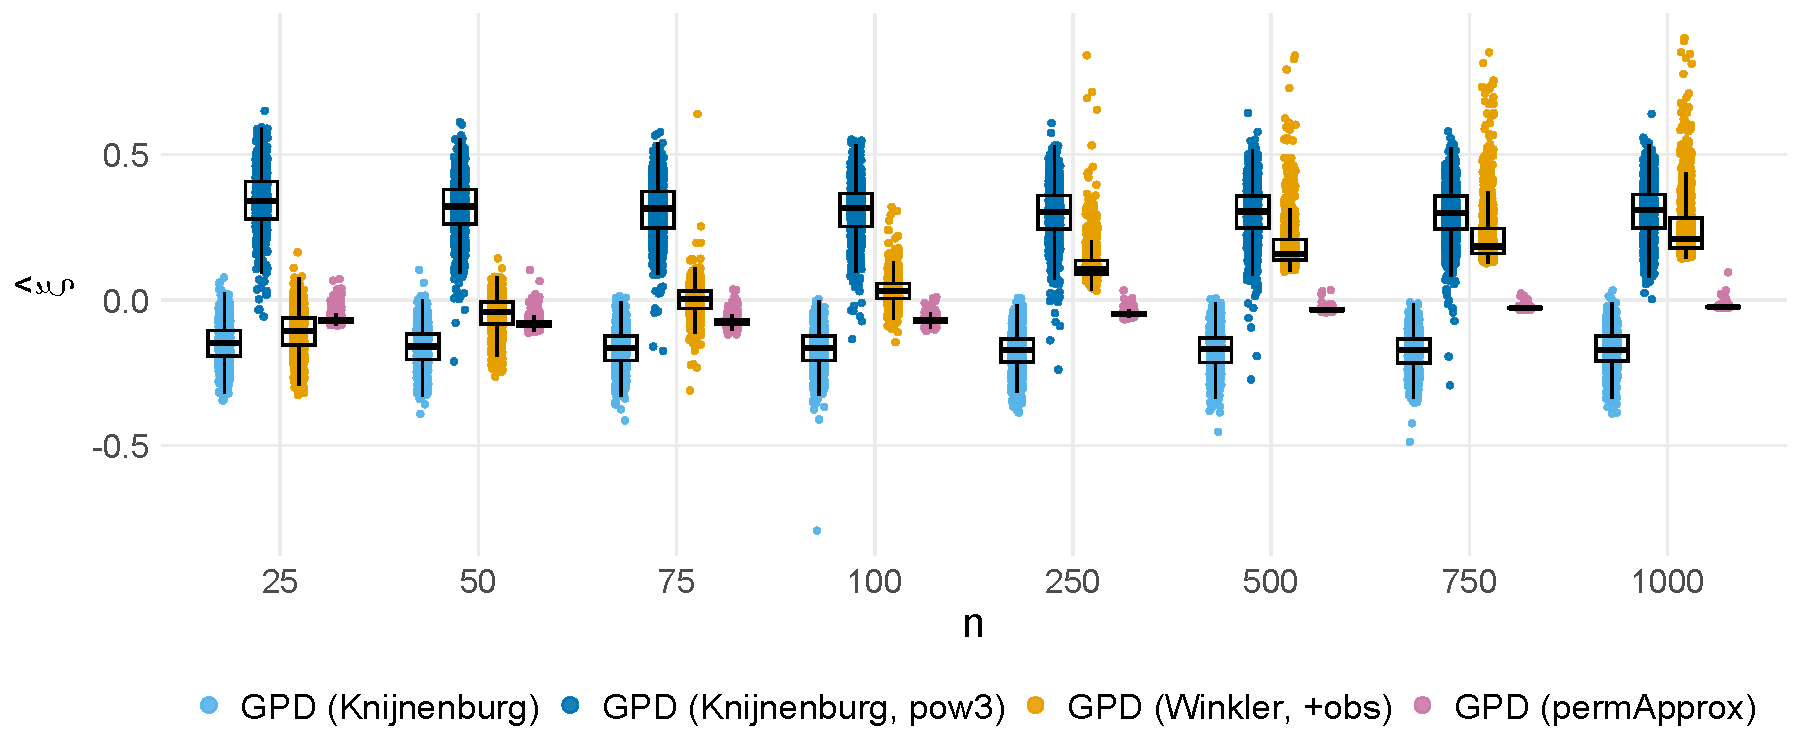
\includegraphics[width=\textwidth]{../ch06_permapprox/simulations/perm_ttest/figures/05_p_approx_methods/sim_ttest_papprox_shape_estimates_by_n-1.pdf}
  \caption{\textbf{Two-sample t-test with Gaussian data:} Estimated GPD shape values across sample sizes for the compared GPD-based methods. Effect size and number of permutations are fixed to $d=1$ and $B=1000$, respectively. Points indicate individual replicates (1000 per setting).}
  \label{fig:app:6perm:ttest_shapes_by_n}
\end{figure}

% t-test: p-values by n
\begin{figure}[ht]
  \centering
  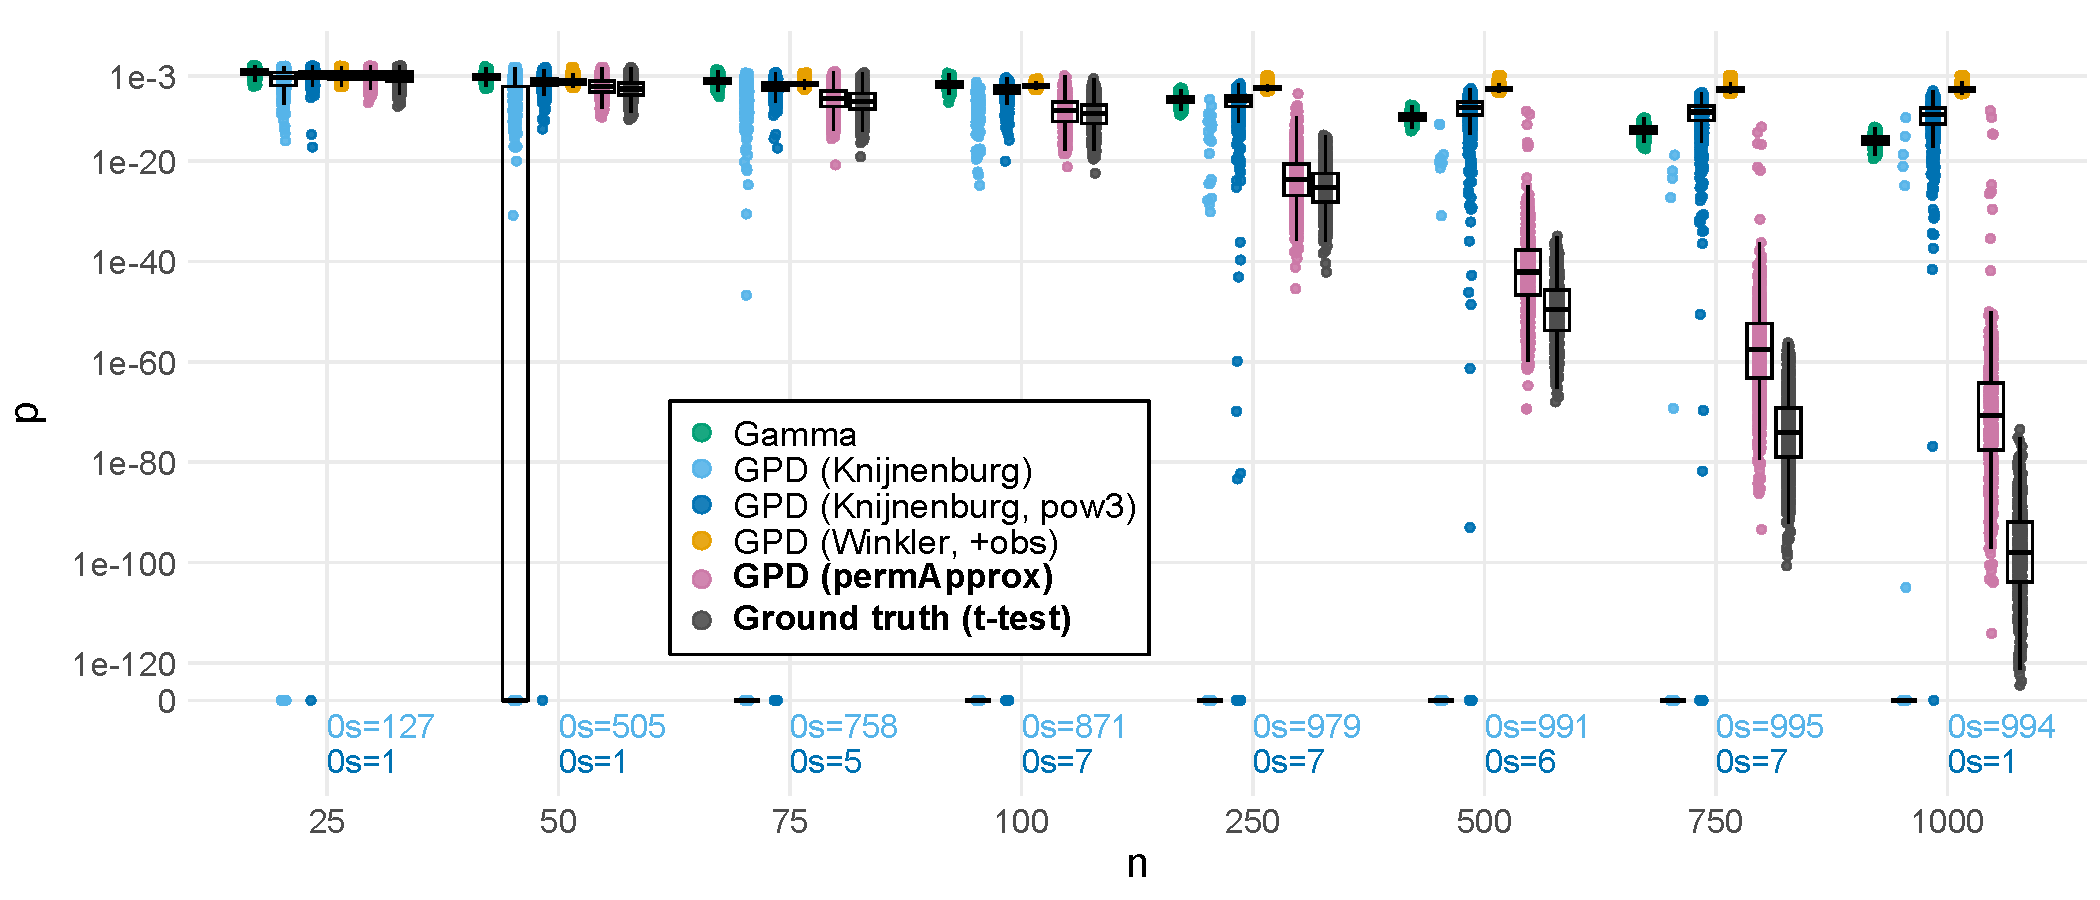
\includegraphics[width=\textwidth]{../ch06_permapprox/simulations/perm_ttest/figures/05_p_approx_methods/sim_ttest_papprox_pvals_by_n-1.pdf}
  \caption{\textbf{Two-sample t-test with Gaussian data:} $p$-values produced with the different approximation methods, in comparison to Student's \textit{t}-test $p$-values across varying sample sizes.
  Effect size and number of permutations are fixed to $d=1$ and $B=1000$, respectively. Points indicate individual replicates (1000 per setting). 
  Counts of exact zeros are shown below each group as ``\texttt{0s}=x'' in the corresponding color.
  Zero $p$-values are mapped to a small constant floor so they appear at ``0'' on the $y$-axis. The y-axis is on a log10 scale, while tick labels show the original $p$-values.}
  \label{fig:app:6perm:ttest_pvals_by_n}
\end{figure}

% t-test: p-values by d and B
\begin{figure}[H]
  \centering
  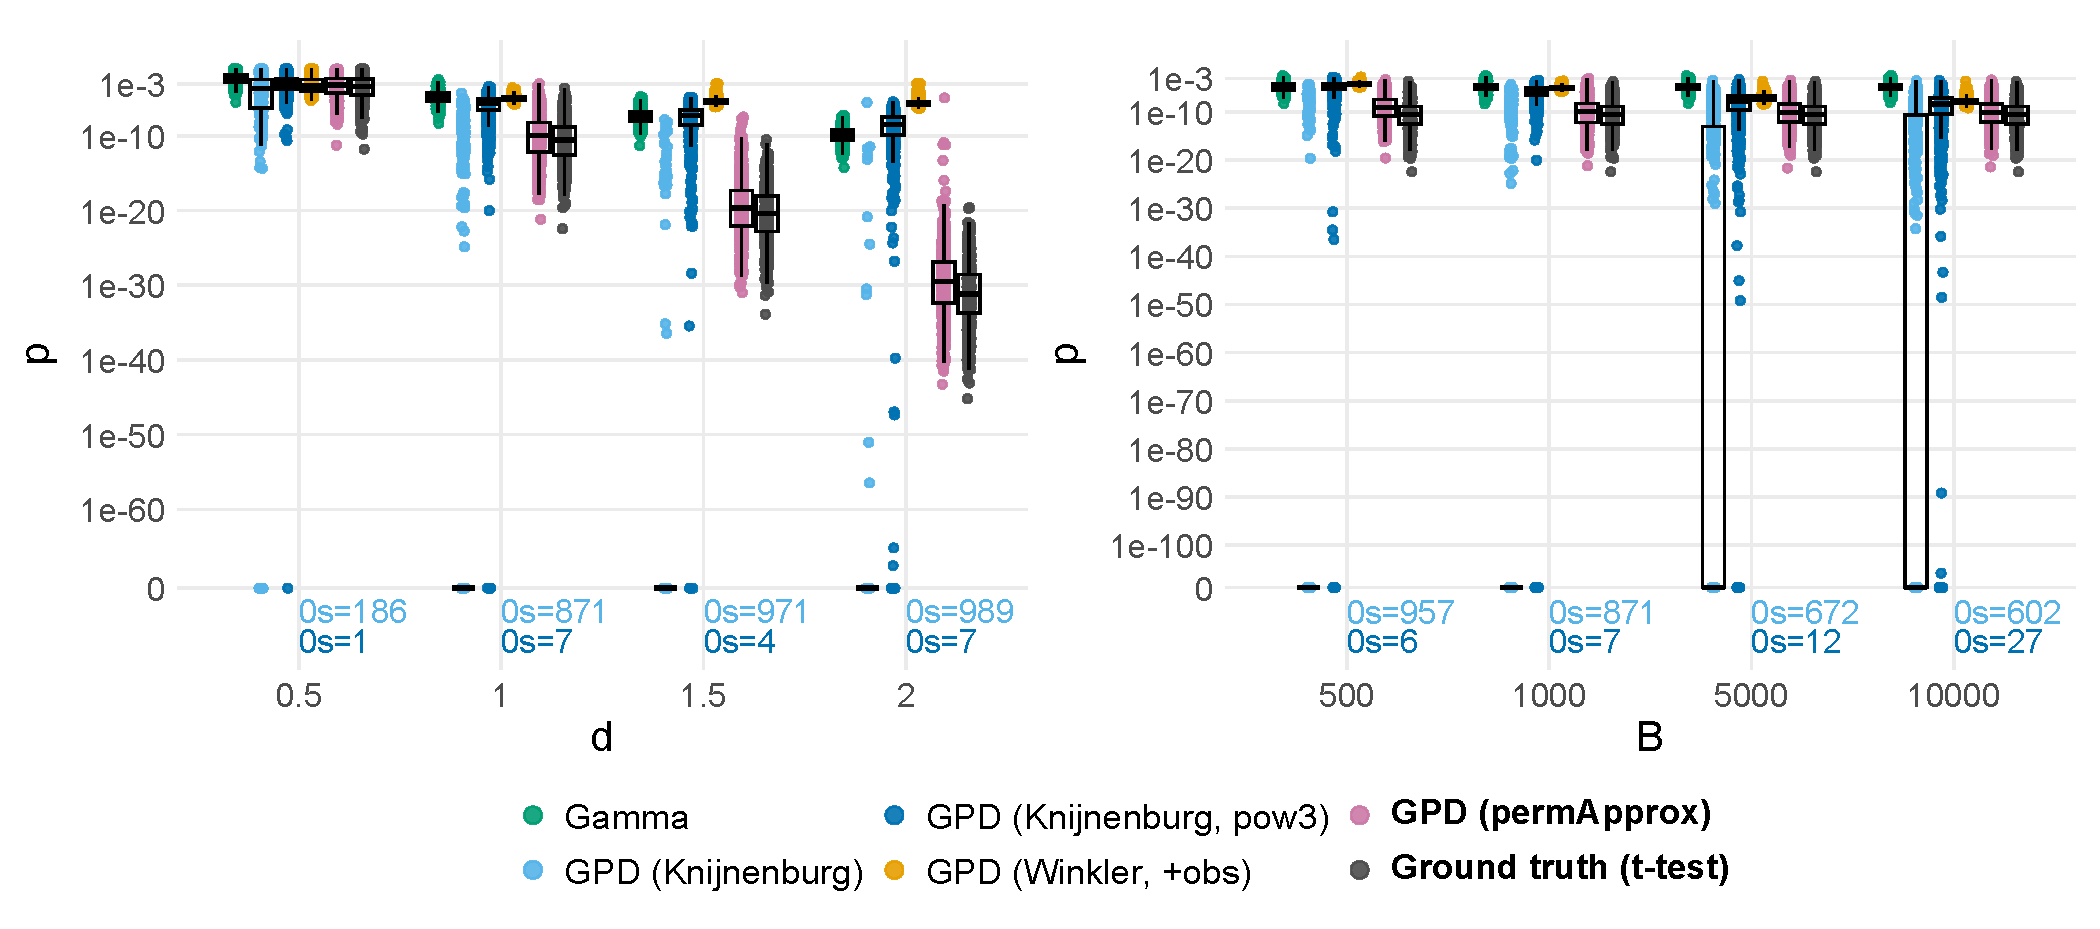
\includegraphics[width=\textwidth]{../ch06_permapprox/simulations/perm_ttest/figures/05_p_approx_methods/sim_ttest_papprox_pvals_by_d_and_B-1.pdf}
  \caption{\textbf{Two-sample t-test with Gaussian data:} Approximated permutation $p$-values, stratified by effect size $d$ (left panel) and number of permutations $B$ (right panel). Fixed values (if not stratified): $n=100$, $d=1$ and $B=1000$. Points indicate individual replicates (1000 per setting). 
  Counts of exact zeros are shown below each group as ``\texttt{0s}=x'' in the corresponding color.
  For plotting only, zero $p$-values are mapped to a small constant floor so they appear at ``0'' on the $y$-axis. The y-axis is on a log10 scale, while tick labels show the original $p$-values.}
  \label{fig:app:6perm:ttest_pvals_by_d_and_B}
\end{figure}

% t-test: ratios by d and B
\begin{figure}[H]
  \centering
  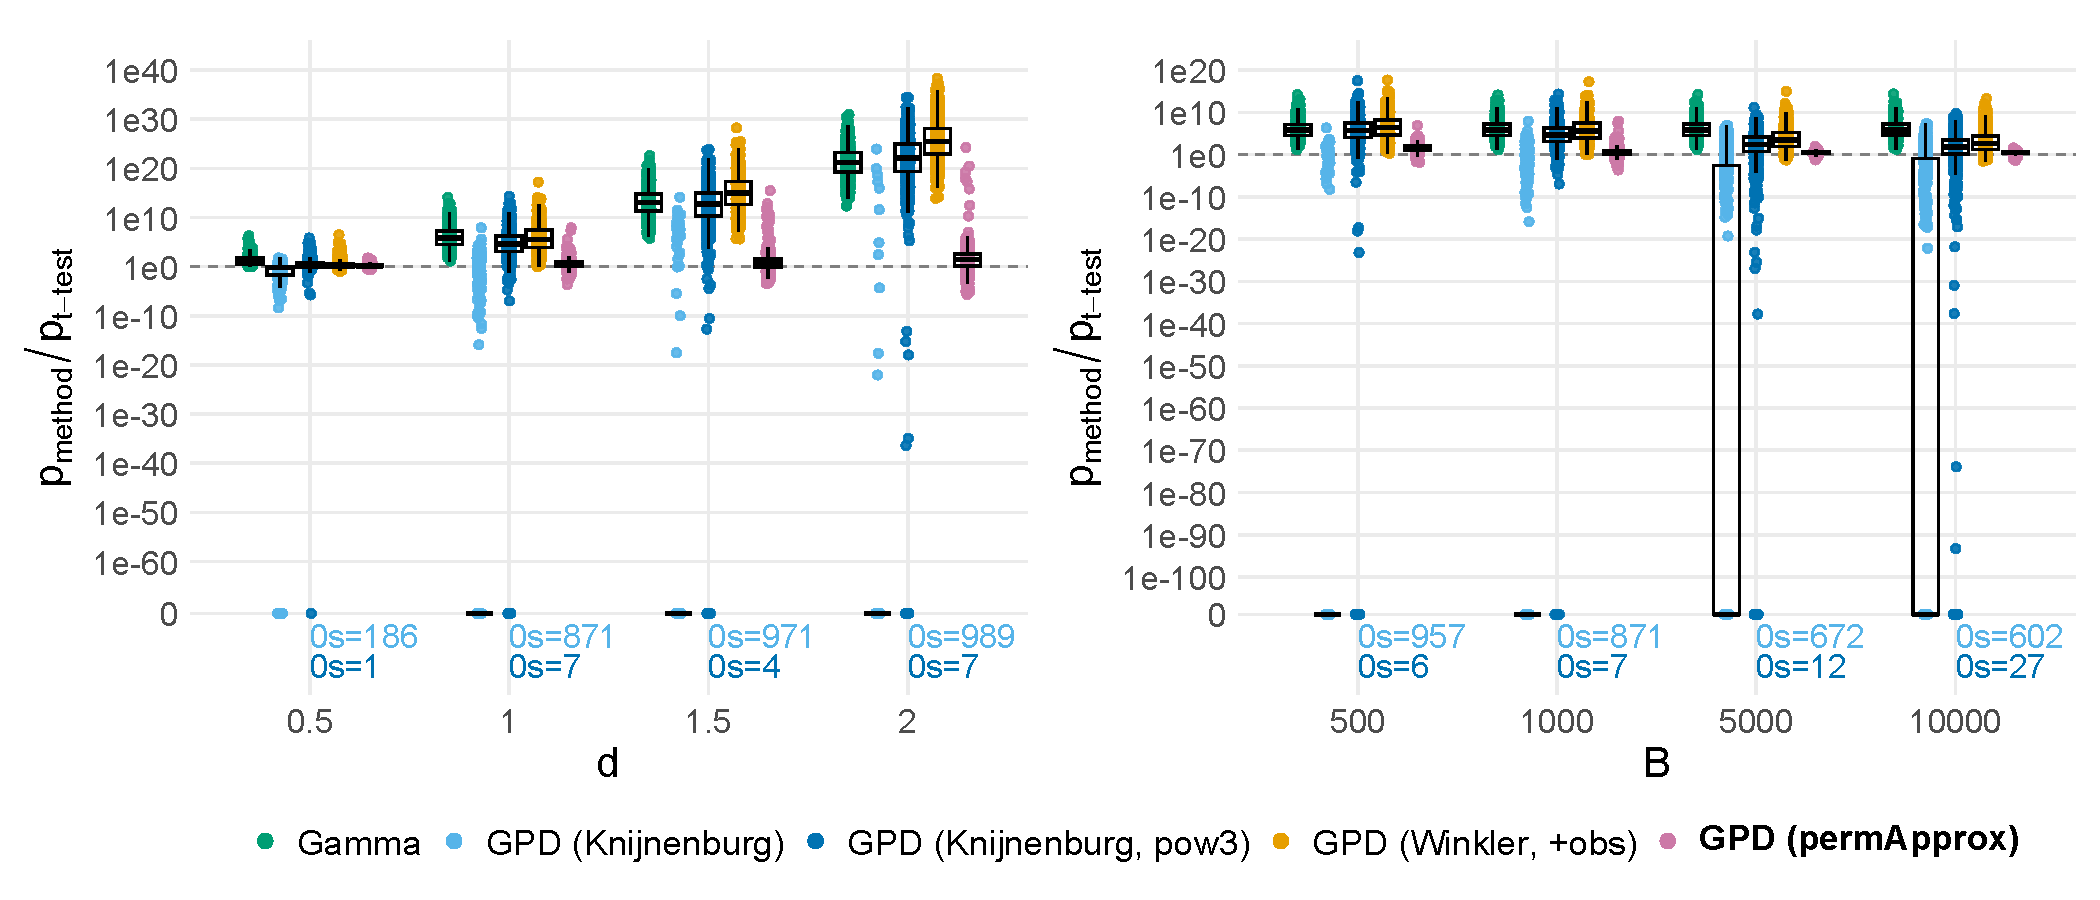
\includegraphics[width=\textwidth]{../ch06_permapprox/simulations/perm_ttest/figures/05_p_approx_methods/sim_ttest_papprox_ratios_by_d_and_B-1.pdf}
  \caption{\textbf{Two-sample t-test with Gaussian data:} Ratios of approximated to ground-truth $p$-values: $p_{\text{method}} / p_{t\text{-test}}$, stratified by effect size $d$ (left panel) and number of permutations $B$ (right panel). Fixed values (if not stratified): $n=100$, $d=1$ and $B=1000$. Points indicate individual replicates (1000 per setting). 
  Counts of exact zeros are shown below each group as ``\texttt{0s}=x'' in the corresponding color.
  For plotting only, zero $p$-values are mapped to a small constant floor so they appear at ``0'' on the $y$-axis ratios.}
  \label{fig:app:6perm:ttest_ratios_by_d_and_B}
\end{figure}

% Wilcoxon: p-values by n
\begin{figure}[H]
  \centering
  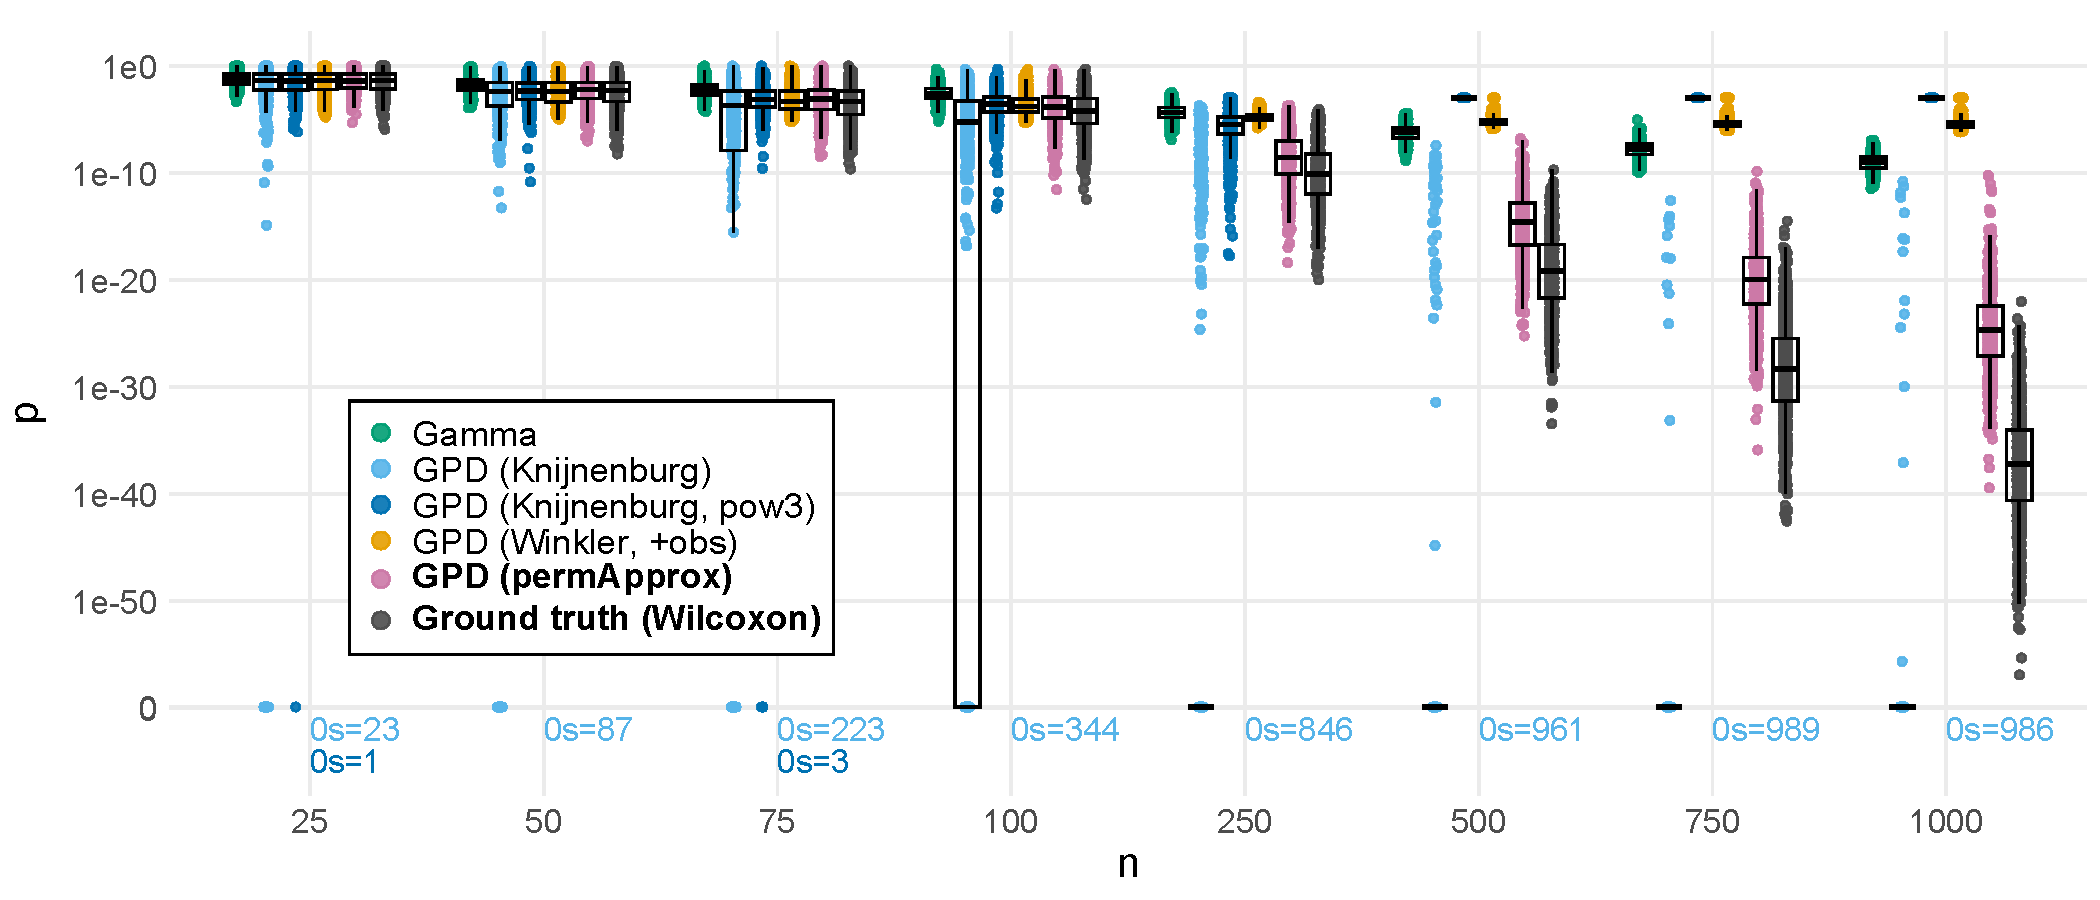
\includegraphics[width=\textwidth]{../ch06_permapprox/simulations/perm_wilcox/figures/02_p_approx_methods/sim_wilcox_papprox_pvals_by_n-1.pdf}
    \caption{\textbf{Wilcoxon rank-sum test with exponential data:} Approximated permutation $p$-values, stratified by sample size $n$. Fixed values: $d=1$ and $B=1000$. Points indicate individual replicates (1000 per setting). 
    Counts of exact zeros are shown below each group as ``\texttt{0s}=x'' in the corresponding color. 
    For plotting only, zero $p$-values are mapped to a small constant floor so they appear at ``0'' on the $y$-axis. The y-axis is on a log10 scale, while tick labels show the original $p$-values.}
  \label{fig:app:6perm:wilcox_pvals_by_n}
\end{figure}

% Wilcoxon: p-values by d and B
\begin{figure}[H]
  \centering
  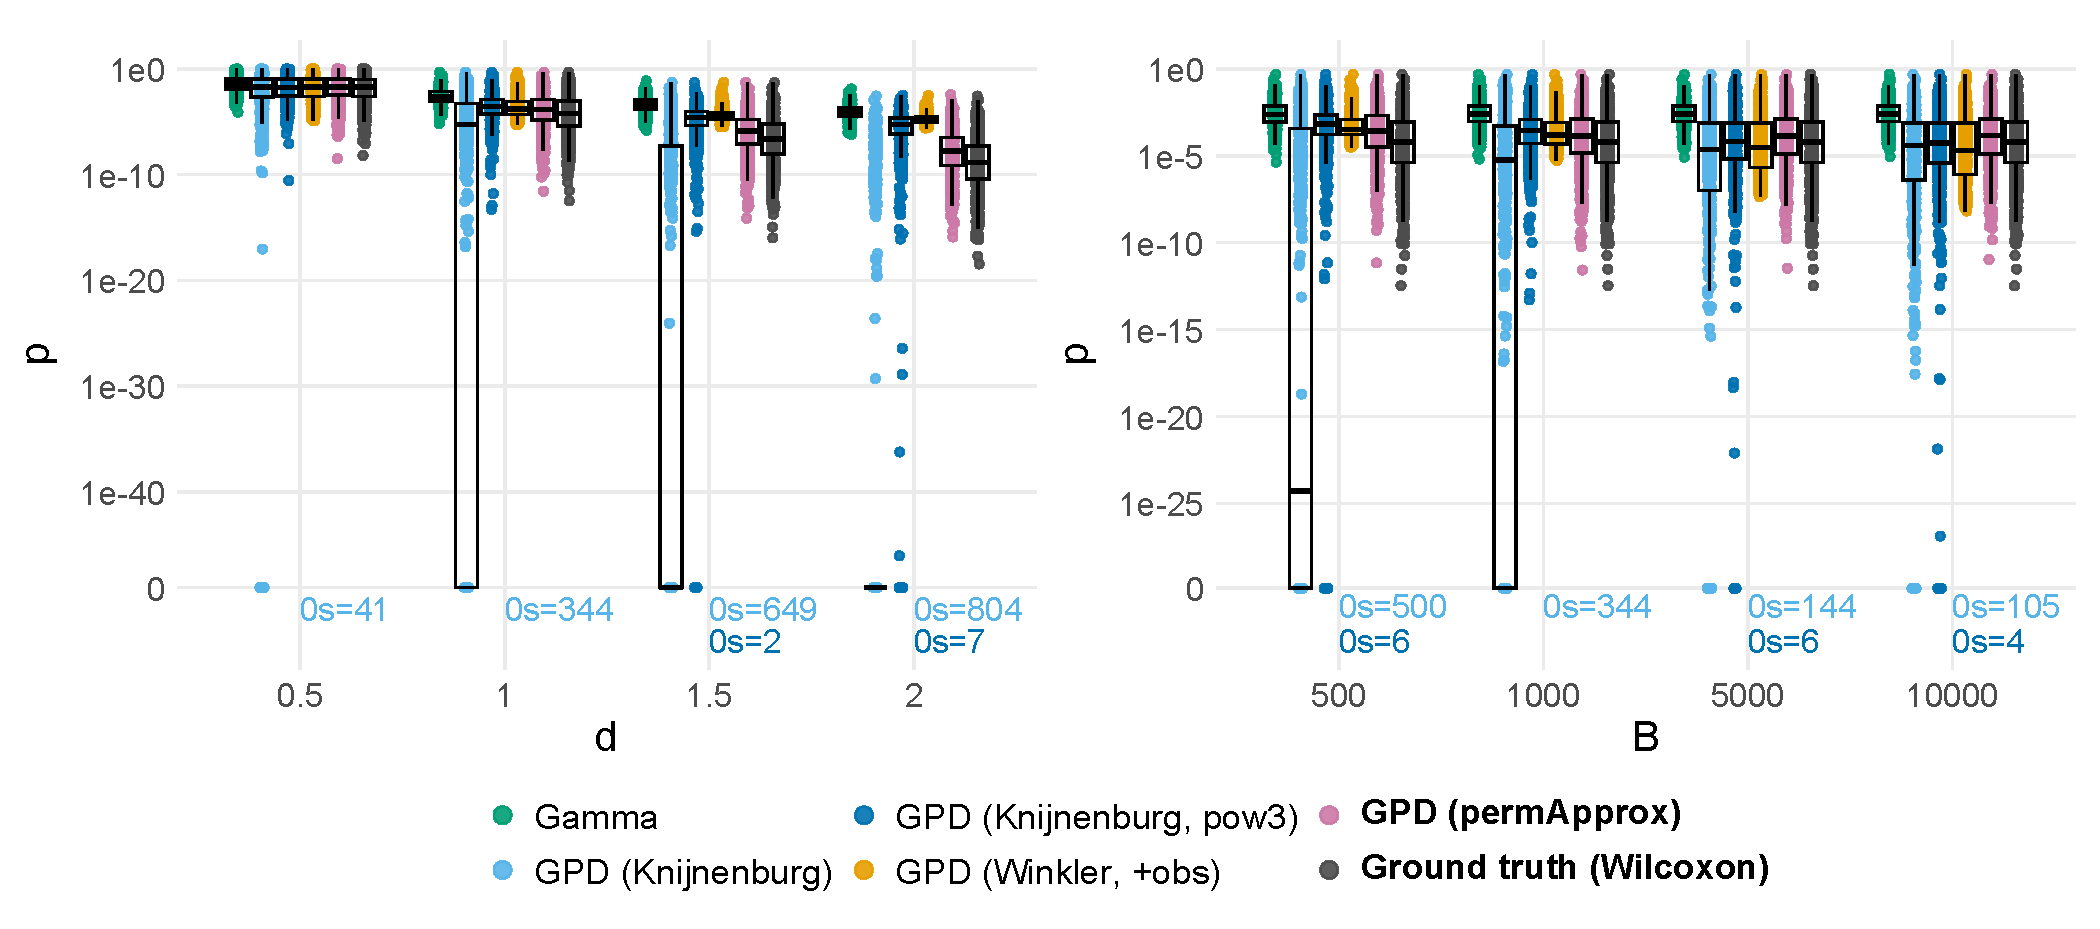
\includegraphics[width=\textwidth]{../ch06_permapprox/simulations/perm_wilcox/figures/02_p_approx_methods/sim_wilcox_papprox_pvals_by_d_and_B-1.pdf}
  \caption{\textbf{Wilcoxon rank-sum test with exponential data:} Approximated permutation $p$-values, stratified by effect size $d$ (left panel) and number of permutations $B$ (right panel). Fixed values (if not stratified): $n=100$, $d=1$ and $B=1000$. Points indicate individual replicates (1000 per setting). 
  Counts of exact zeros are shown below each group as ``\texttt{0s}=x'' in the corresponding color.
  For plotting only, zero $p$-values are mapped to a small constant floor so they appear at ``0'' on the $y$-axis. The y-axis is on a log10 scale, while tick labels show the original $p$-values.}
  \label{fig:app:6perm:wilcox_pvals_by_d_and_B}
\end{figure}

% Wilcoxon: ratios by d and B
\begin{figure}[H]
  \centering
  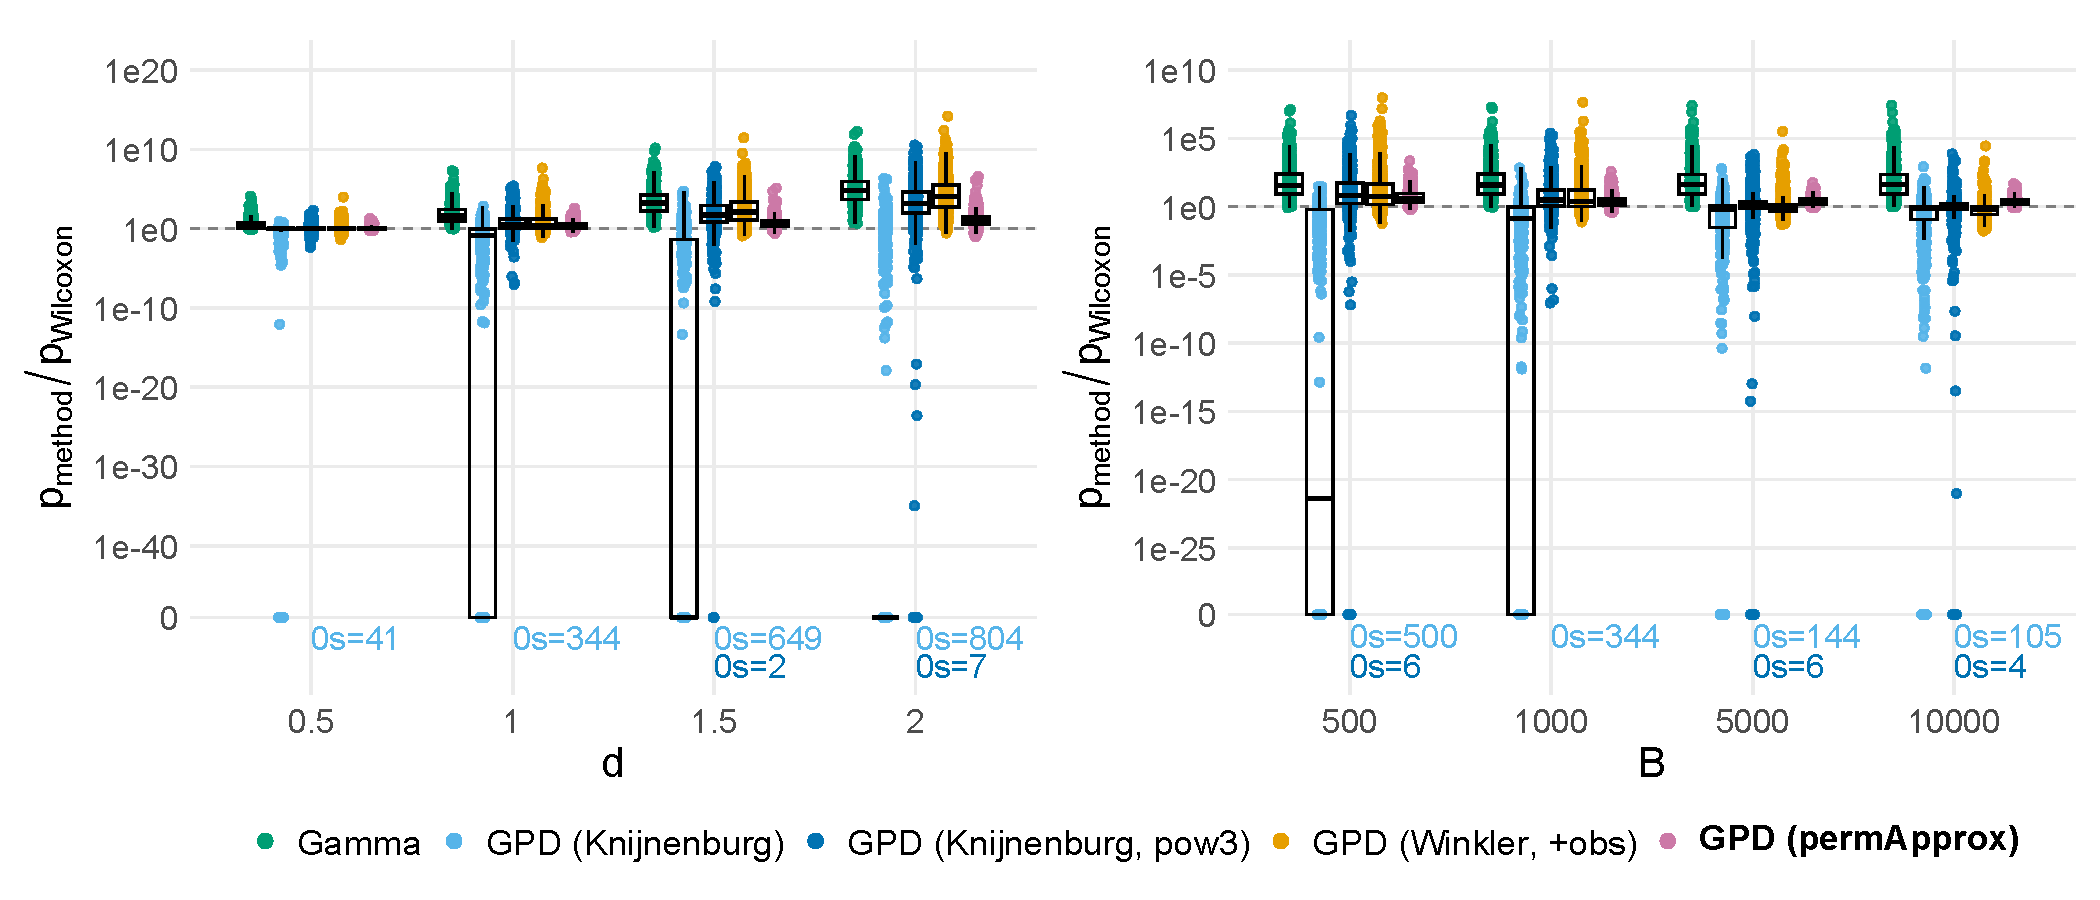
\includegraphics[width=\textwidth]{../ch06_permapprox/simulations/perm_wilcox/figures/02_p_approx_methods/sim_wilcox_papprox_ratios_by_d_and_B-1.pdf}
  \caption{\textbf{Wilcoxon rank-sum test with exponential data:} Ratios of approximated to ground-truth $p$-values: $p_{\text{Method}} / p_{\text{Wilcoxon}}$, stratified by effect size $d$ (left panel) and number of permutations $B$ (right panel). Fixed values (if not stratified): $n=100$, $d=1$ and $B=1000$. Points indicate individual replicates (1000 per setting). 
  Counts of exact zeros are shown below each group as ``\texttt{0s}=x'' in the corresponding color.
  For plotting only, zero $p$-values are mapped to a small constant floor so they appear at ``0'' on the $y$-axis. The y-axis is on a log10 scale, while tick labels show the original ratios.}
  \label{fig:app:6perm:wilcox_ratios_by_d_and_B}
\end{figure}

% !TeX root = ../thesis.tex
\chapter{Appendices to Chapter 7 (PASTURE analysis)}
\label{sec:app:application}

%====================================
\section{Within-sample diversity across remaining cohort variables}
\label{sec:app:7app:alpha_remaining}
%====================================

The following figures show within-sample diversity estimates for the cohort variables that were not selected as the main grouping variable in Chapter~\ref{ch:application}. Richness was estimated using \texttt{breakaway}, whereas Shannon diversity and the Gini--Simpson index were estimated using \texttt{DivNet}. For each variable and diversity measure, an overall Kruskal--Wallis test was performed first using the standard asymptotic approximation. If the overall test was significant and the variable had more than two groups, pairwise Wilcoxon rank-sum tests were carried out for all group combinations. For variables with two groups, the Wilcoxon rank-sum test corresponds to the group comparison shown in the figure. Reported p-values are asymptotic p-values and are displayed only for significant comparisons.

%------------------------------------
% alpha diversity: country
%------------------------------------
\begin{figure}[H]
\centering
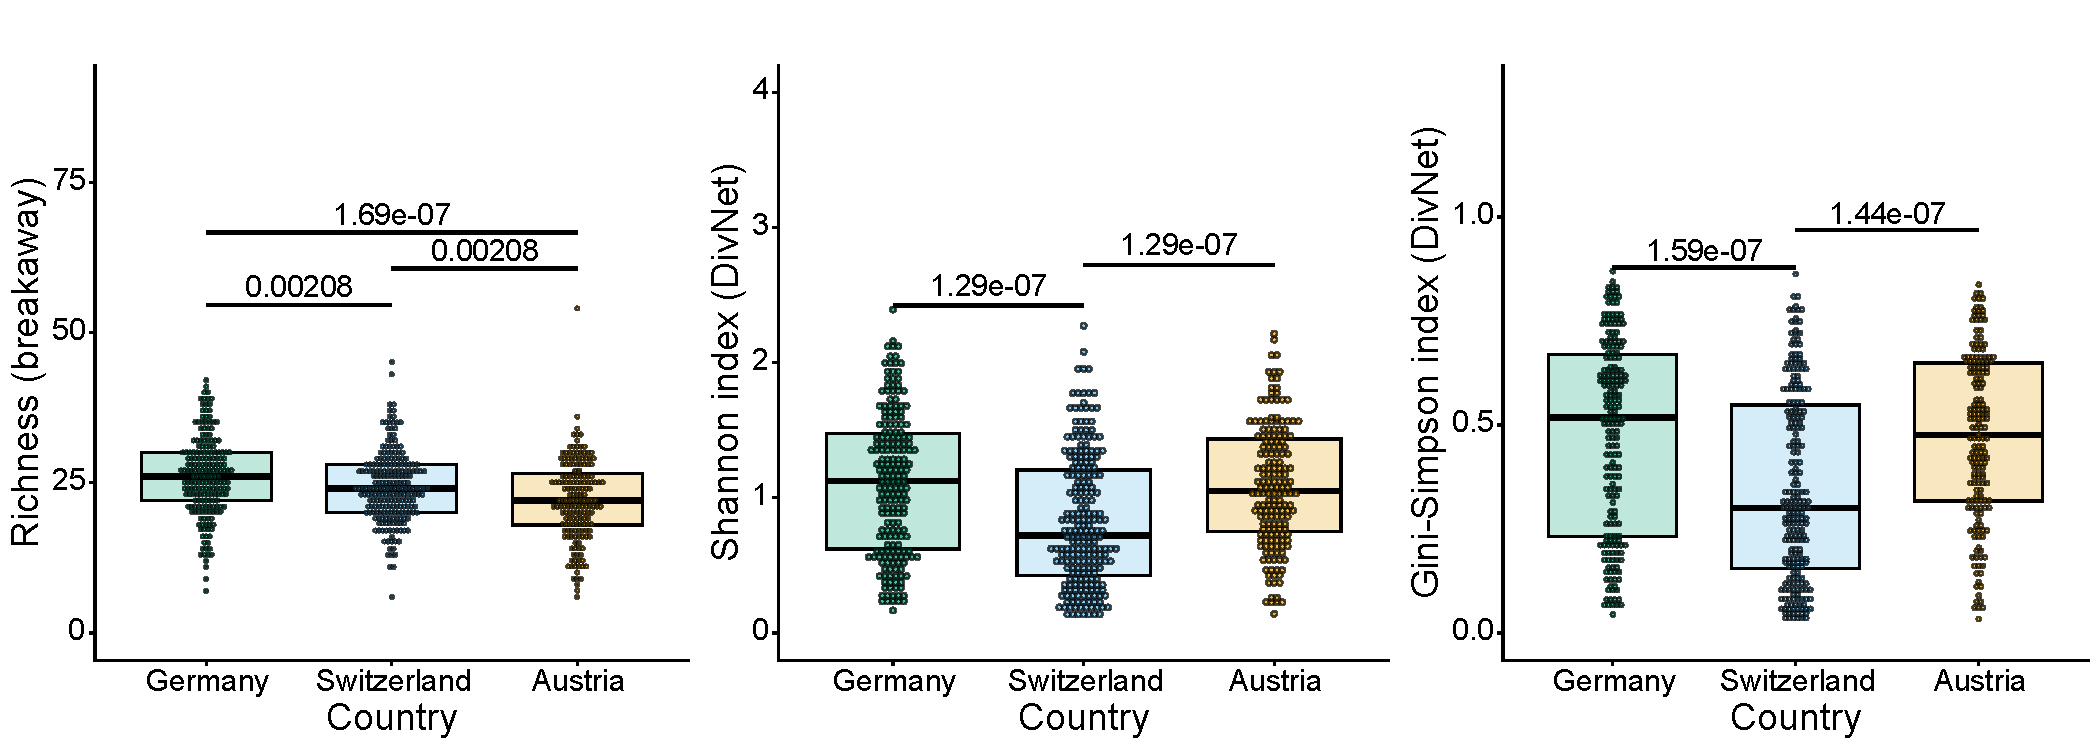
\includegraphics[width=\textwidth]{../ch07_application/figures/03_alpha_diversity/Country_2m-1.pdf}
\caption{\textbf{Within-sample diversity by country.} Sample-wise estimates of richness, Shannon diversity, and Gini--Simpson diversity stratified by country. Sample sizes are 173 for Austria, 197 for Germany, and 222 for Switzerland.}
\label{fig:app:7app:alpha_div_country}
\end{figure}

%------------------------------------
% alpha diversity: sex
%------------------------------------
\begin{figure}[H]
\centering
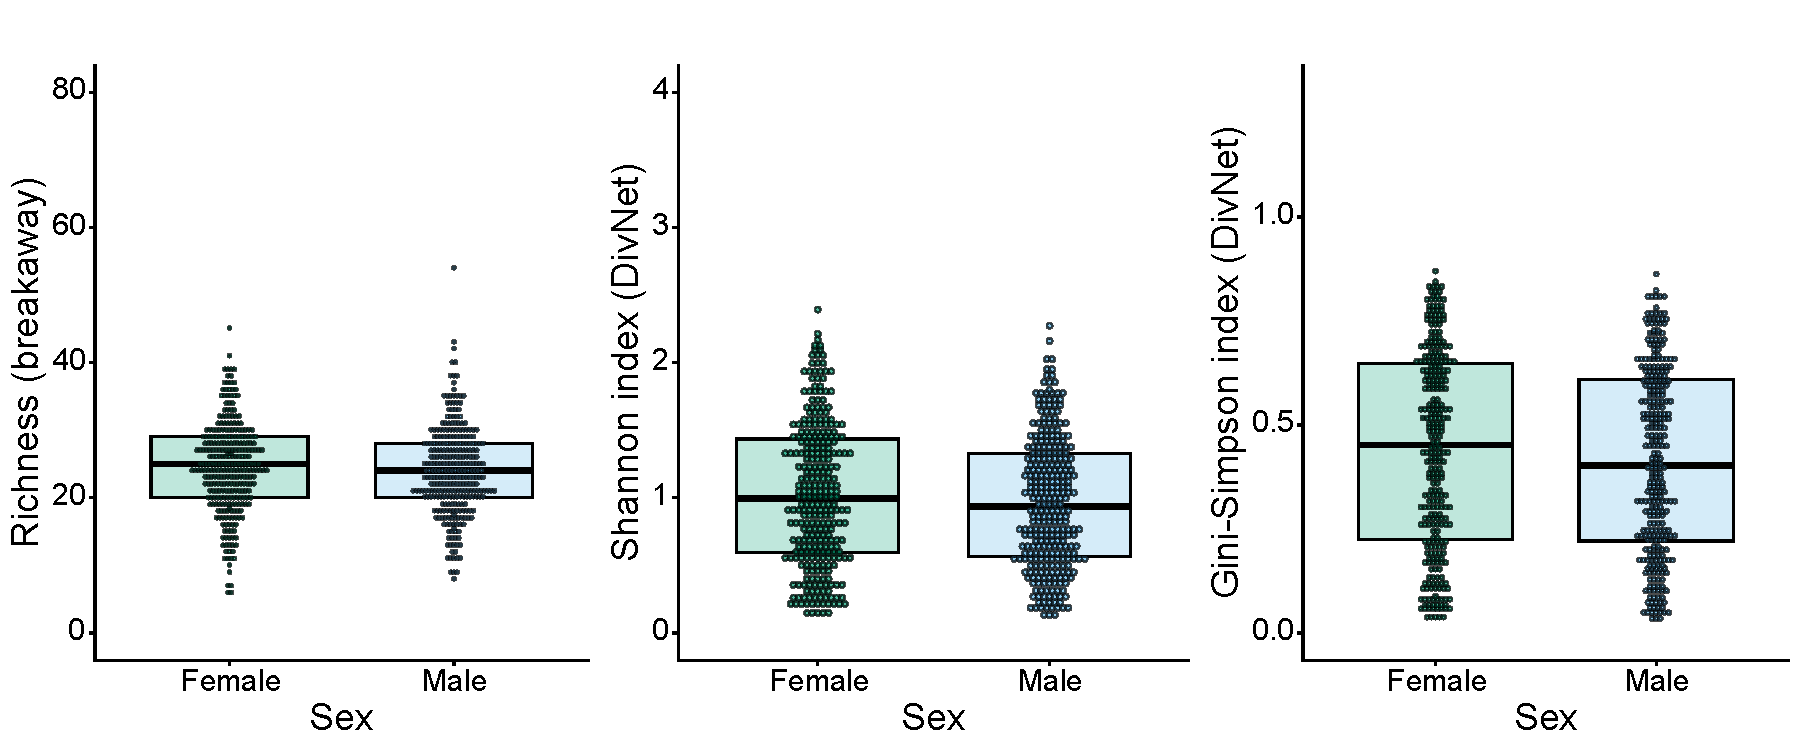
\includegraphics[width=\textwidth]{../ch07_application/figures/03_alpha_diversity/sex_2m-1.pdf}
\caption{\textbf{Within-sample diversity by sex.} Sample-wise estimates of richness, Shannon diversity, and Gini--Simpson diversity stratified by child sex. Sample sizes are 294 for female and 298 for male children.}
\label{fig:app:7app:alpha_div_sex}
\end{figure}

%------------------------------------
% alpha diversity: delivery mode
%------------------------------------
\begin{figure}[H]
\centering
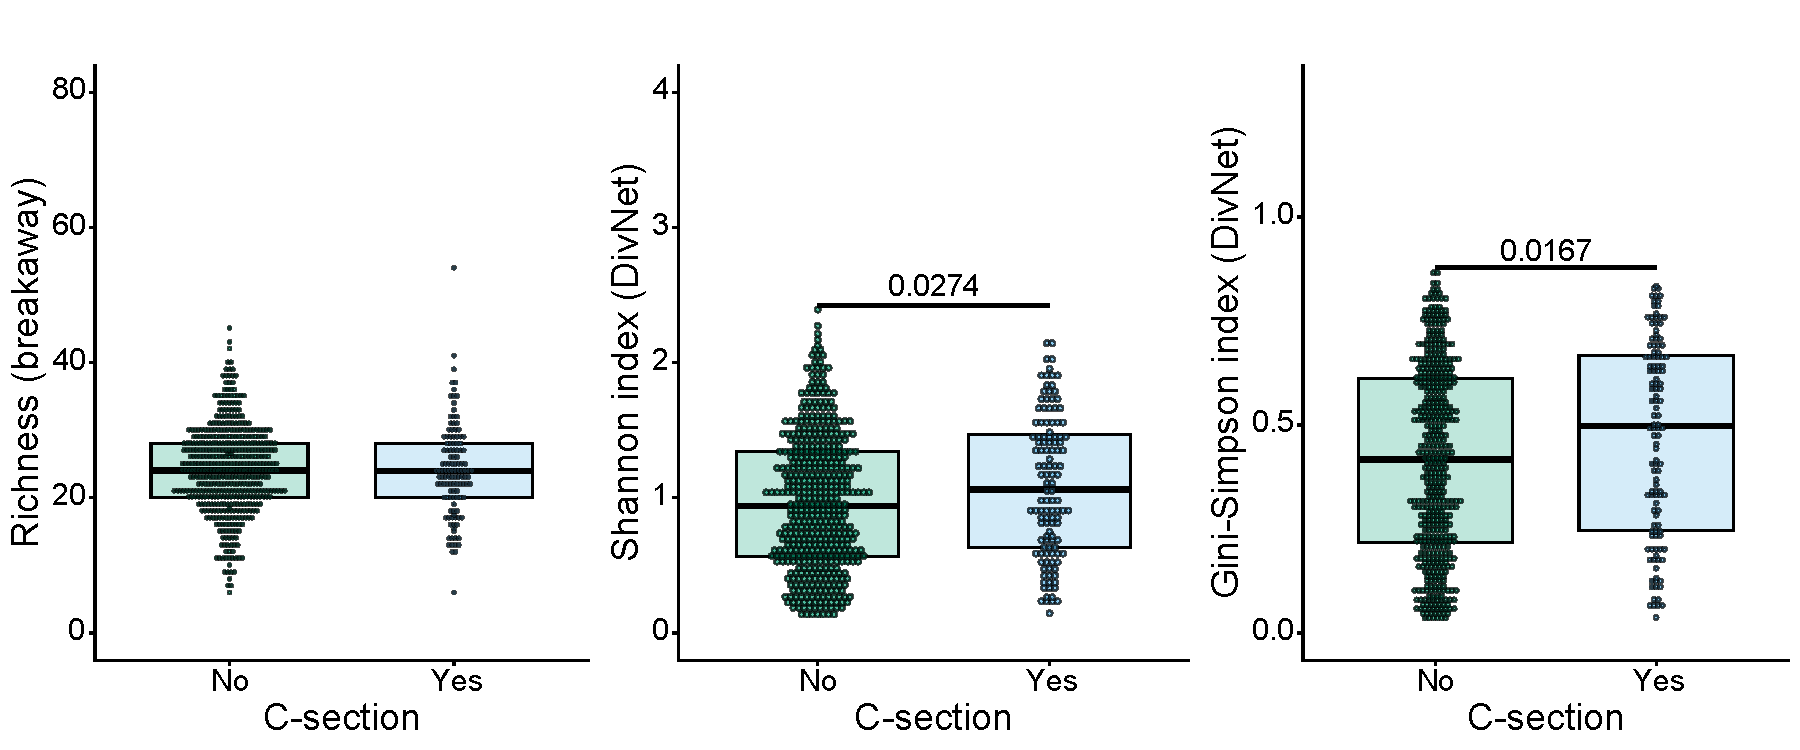
\includegraphics[width=\textwidth]{../ch07_application/figures/03_alpha_diversity/cesarean_2m-1.pdf}
\caption{\textbf{Within-sample diversity by delivery mode.} Sample-wise estimates of richness, Shannon diversity, and Gini--Simpson diversity stratified by delivery mode. Sample sizes are 468 for vaginal delivery and 121 for delivery by cesarean section.}
\label{fig:app:7app:alpha_div_csection}
\end{figure}

%------------------------------------
% alpha diversity: breastfeeding duration
%------------------------------------
\begin{figure}[H]
\centering
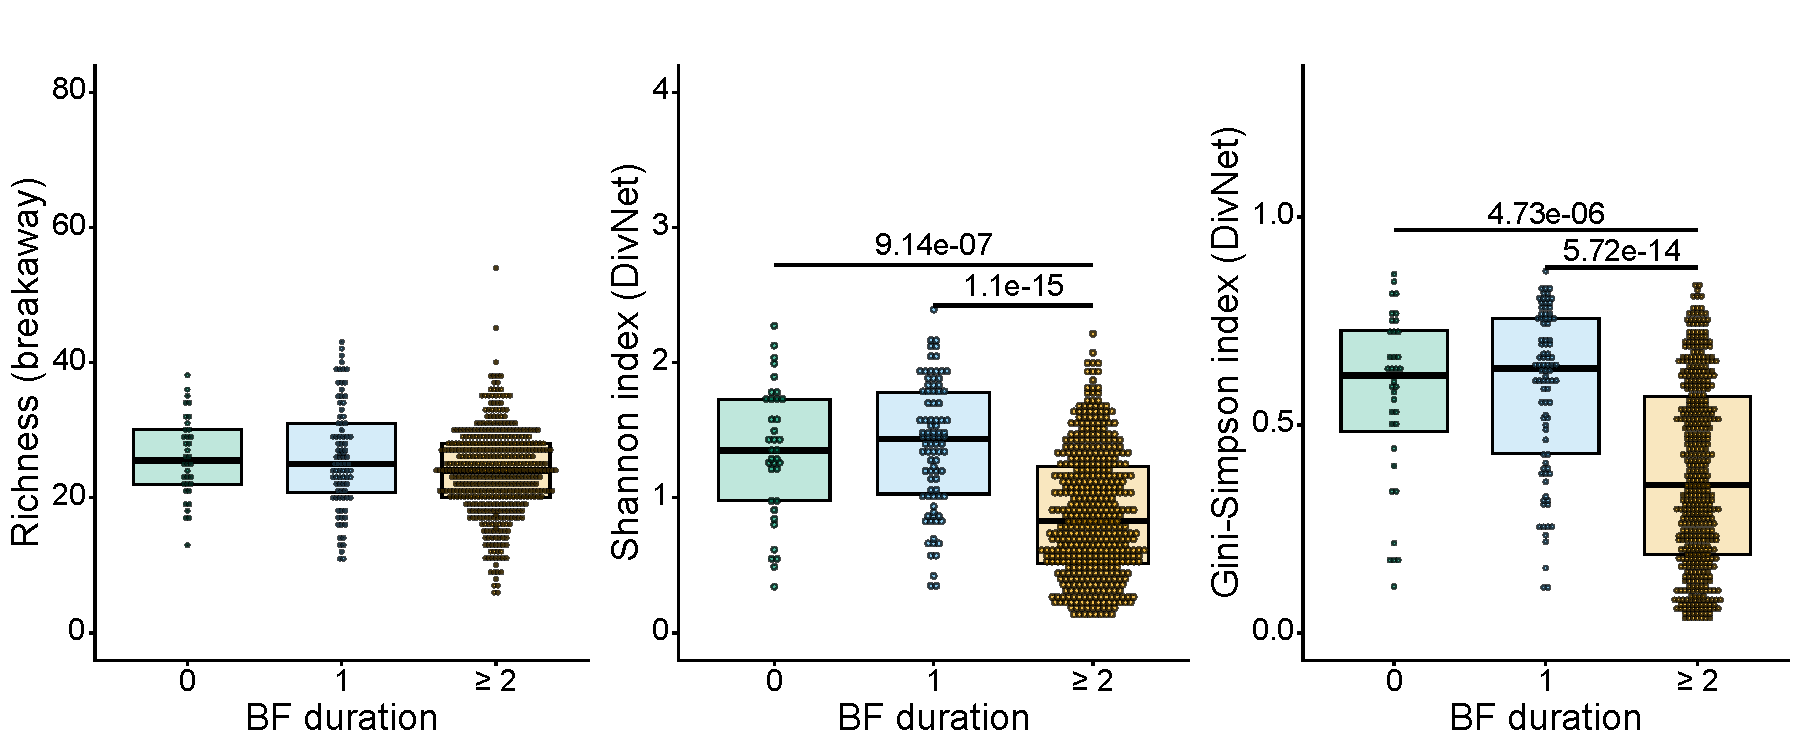
\includegraphics[width=\textwidth]{../ch07_application/figures/03_alpha_diversity/breastfeed_2m-1.pdf}
\caption{\textbf{Within-sample diversity by breastfeeding duration.} Sample-wise estimates of richness, Shannon diversity, and Gini--Simpson diversity stratified by total breastfeeding duration. Sample sizes are 36 for no breastfeeding, 88 for one month of breastfeeding, and 456 for at least two months of breastfeeding.}
\label{fig:app:7app:alpha_div_bf_duration}
\end{figure}

%------------------------------------
% alpha diversity: prenatal smoking
%------------------------------------
\begin{figure}[H]
\centering
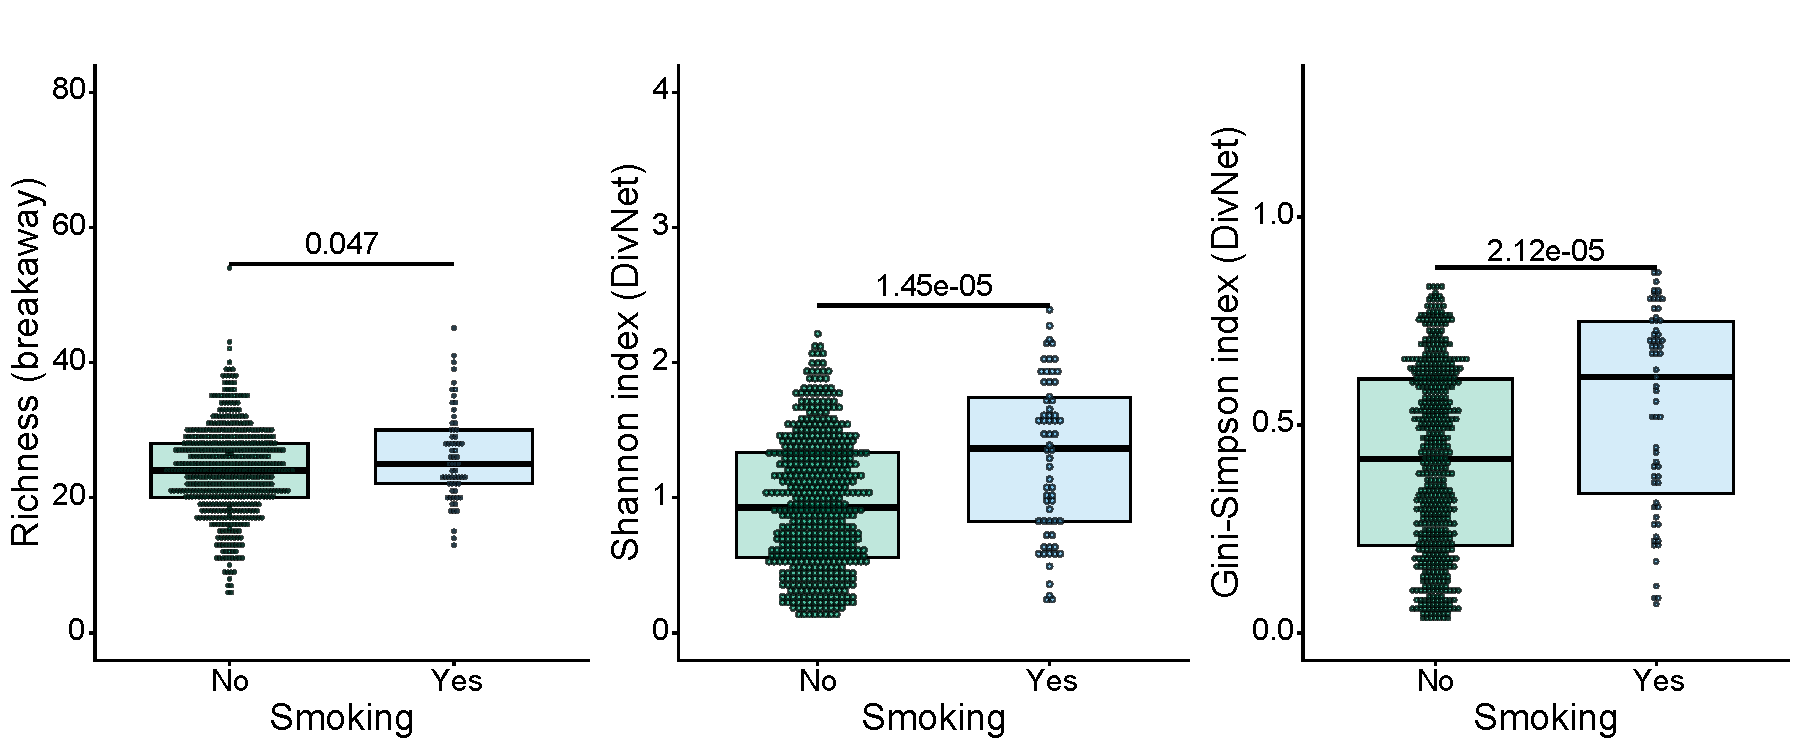
\includegraphics[width=\textwidth]{../ch07_application/figures/03_alpha_diversity/pregsmoke_2m-1.pdf}
\caption{\textbf{Within-sample diversity by prenatal smoking.} Sample-wise estimates of richness, Shannon diversity, and Gini--Simpson diversity stratified by maternal smoking during pregnancy. Sample sizes are 529 for no prenatal smoking and 63 for prenatal smoking.}
\label{fig:app:7app:alpha_div_smoking}
\end{figure}

%------------------------------------
% alpha diversity: number of older siblings
%------------------------------------
\begin{figure}[H]
\centering
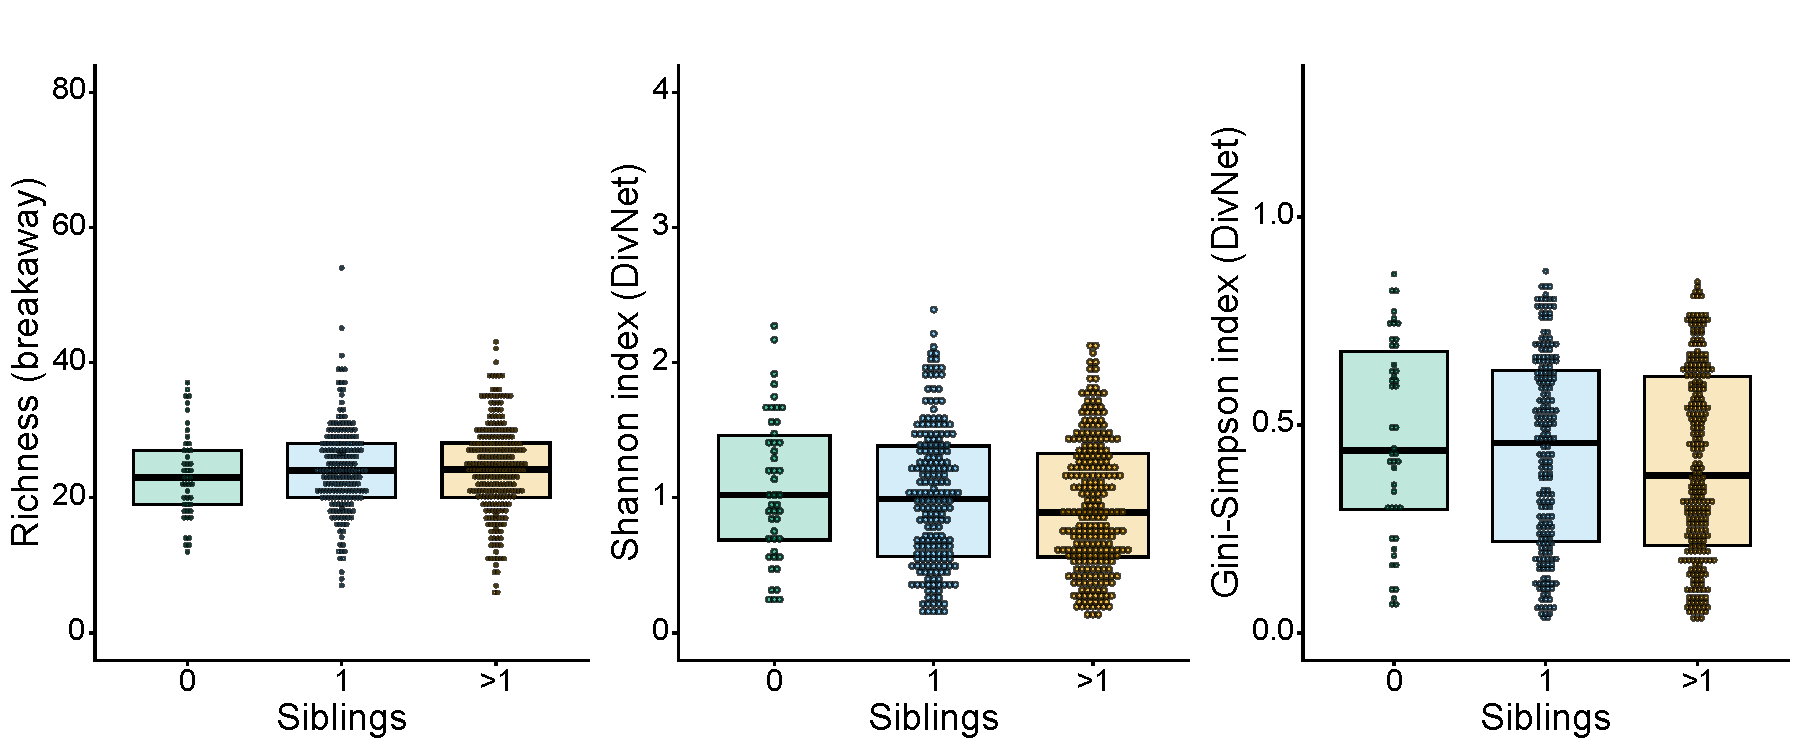
\includegraphics[width=\textwidth]{../ch07_application/figures/03_alpha_diversity/sibsnumb_2m-1.pdf}
\caption{\textbf{Within-sample diversity by number of older siblings.} Sample-wise estimates of richness, Shannon diversity, and Gini--Simpson diversity stratified by the number of older siblings. Sample sizes are 46 for no older siblings, 200 for one older sibling, and 257 for more than one older sibling.}
\label{fig:app:7app:alpha_div_siblings}
\end{figure}

%====================================
\section{Compositional equivalence}
\label{sec:app:7app:comp_equivalence}
%====================================

\begin{figure}[H]
\centering
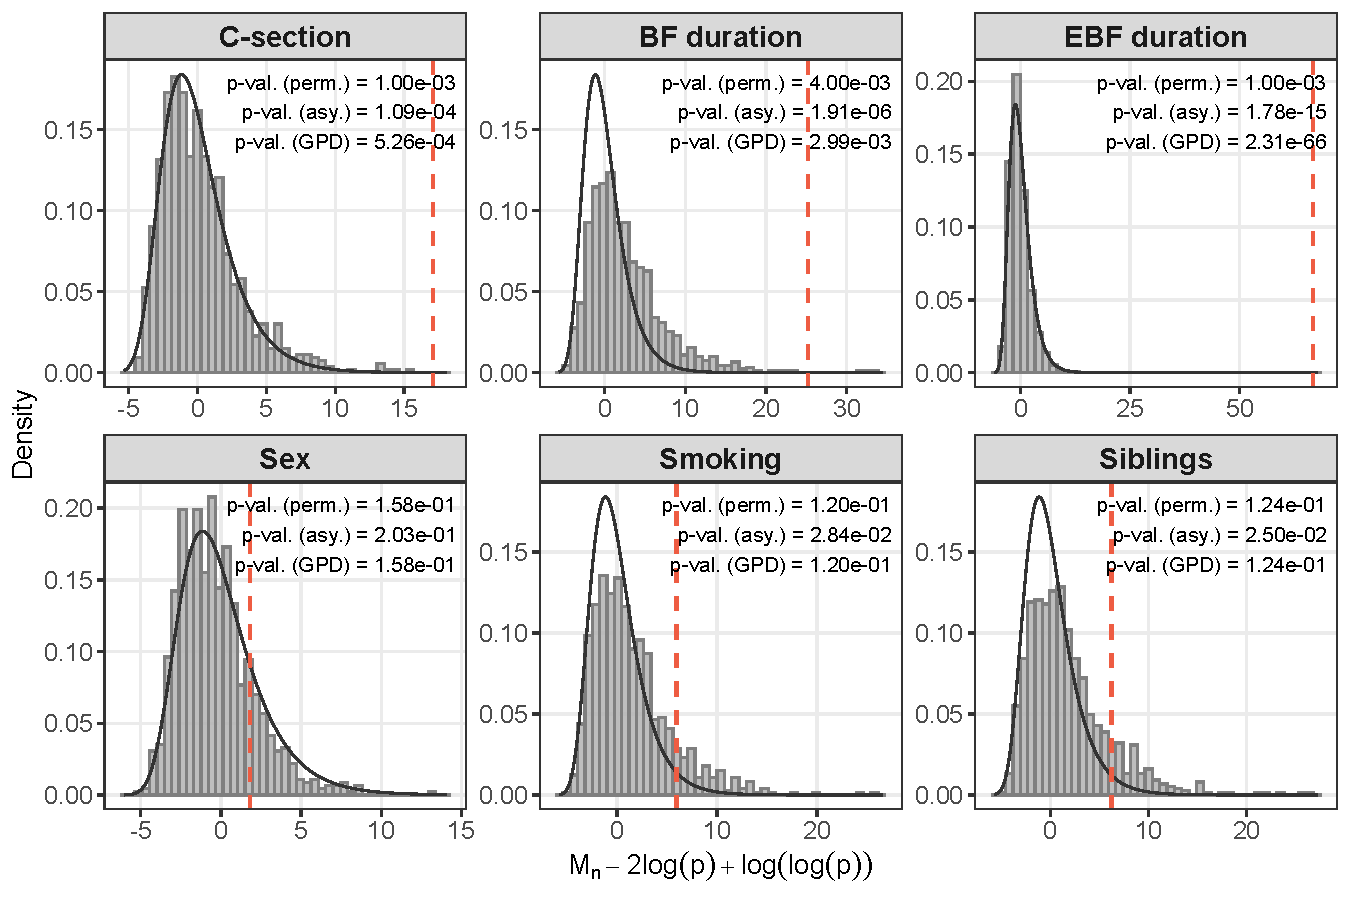
\includegraphics[width=\textwidth]{../ch07_application/figures/06_comp_equivalence/comp_equivalence_gumbel_comparison_plot-1.pdf}
\caption{\textbf{Comparison of permutation-based and asymptotic null distributions for compositional equivalence.}
For each selected two-group contrast, the gray histogram shows the permutation distribution of the centered statistic $M_n - 2\log(p) + \log\log(p)$, where $M_n$ is the maximum standardized squared CLR mean difference and $p$ is the number of tested CLR coordinates. The gray curve shows the asymptotic Gumbel density proposed by \citet{cao2018twosample}, and the red dashed line marks the observed centered statistic. Annotated p-values show the empirical permutation p-value, the asymptotic Gumbel p-value, and the GPD-refined permutation p-value obtained with \texttt{permApprox}. The comparison illustrates that the asymptotic Gumbel approximation does not uniformly match the permutation null distributions for the PASTURE contrasts.}
\label{fig:app:7app:comp_equivalence_gumbel_comparison}
\end{figure}

%====================================
\section{Differential abundance analysis}
\label{sec:app:7app:diff_abundance}
%====================================

\begin{table}[H]
\centering
\caption{textbf{Adjusted p-values for selected differential abundance analyses.} The table shows genera with Benjamini--Hochberg-adjusted p-values below $\alpha=0.01$ in at least one selected differential abundance analysis. Rows are ordered by increasing adjusted \texttt{permApprox} p-values. The DACOMP statistic $T$ is the observed test statistic used for the permutation test. DACOMP columns show adjusted empirical permutation p-values with the indicated number of permutations, and the \texttt{permApprox} column shows adjusted p-values obtained from constrained GPD tail approximation based on the $1000$-permutation DACOMP run.}
\label{tab:app:7app:diff_abundance_adj_pvalues}\
\vspace{0.5em}
\small
\begin{tabular}{lrlll}
\toprule
Taxon & $T$ & DACOMP ($10^3$) & DACOMP ($10^7$) & \texttt{permApprox} \\
\midrule
\emph{Enterococcus} & $75.64$ & 6.77e-03$^{**}$ & 9.80e-07$^{***}$ & 2.34e-94$^{***}$ \\
\emph{Lactococcus} & $28.84$ & 6.77e-03$^{**}$ & 9.80e-07$^{***}$ & 9.85e-25$^{***}$ \\
\emph{Intestinibacter} & $48.86$ & 6.77e-03$^{**}$ & 9.80e-07$^{***}$ & 3.10e-14$^{***}$ \\
\emph{Streptococcus} & $16.66$ & 6.77e-03$^{**}$ & 1.02e-04$^{***}$ & 1.18e-09$^{***}$ \\
\emph{[Clostridium] innocuum group} & $32.17$ & 6.77e-03$^{**}$ & 1.09e-04$^{***}$ & 3.95e-07$^{***}$ \\
\emph{[Ruminococcus] gnavus group} & $32.23$ & 6.77e-03$^{**}$ & 9.80e-07$^{***}$ & 4.97e-07$^{***}$ \\
\emph{Bifidobacterium} & $36.76$ & 6.77e-03$^{**}$ & 9.80e-07$^{***}$ & 2.50e-05$^{***}$ \\
\emph{Blautia} & $20.75$ & 6.77e-03$^{**}$ & 1.29e-03$^{**}$ & 9.17e-05$^{***}$ \\
\emph{Terrisporobacter} & $20.92$ & 6.77e-03$^{**}$ & 1.68e-03$^{**}$ & 1.96e-03$^{**}$ \\
\addlinespace
\emph{uncultured18} & $13.31$ & 1.28e-02$^{*}$ & 2.97e-03$^{**}$ & 5.06e-02 \\
\emph{Clostridium sensu stricto 1} & $8.04$ & 3.40e-02$^{*}$ & 3.53e-03$^{**}$ & 5.48e-02 \\
\emph{Collinsella} & $6.42$ & 4.14e-02$^{*}$ & 2.97e-03$^{**}$ & 7.09e-02 \\
\emph{[Ruminococcus] torque group} & $8.52$ & 1.82e-02$^{*}$ & 2.97e-03$^{**}$ & 9.64e-02 \\
\emph{Sellimonas} & $3.58$ & 1.53e-01 & 7.76e-03$^{**}$ & 1.62e-01 \\
\emph{Tyzzerella} & $4.47$ & 1.25e-01 & 6.80e-04$^{***}$ & 1.75e-01 \\
\bottomrule
\end{tabular}

\begin{minipage}{0.98\textwidth}
\small
Significance codes refer to adjusted p-values: $^{*} q < 0.05$, $^{**} q < 0.01$, and $^{***} q < 0.001$.
\end{minipage}
\end{table}

%====================================
\section{Differential distribution analysis}
\label{sec:app:7app:diff_distribution}
%====================================

\begin{table}[H]
\centering
\caption{\textbf{Adjusted p-values for selected differential distribution analyses.} The table shows Benjamini--Hochberg-adjusted p-values for genera with an adjusted p-value below $\alpha=0.01$ in at least one panel of Figure~\ref{fig:7app:dd:volcano}. The columns correspond to the non-zero Wasserstein component, the zero-prevalence component, the combined two-stage result, and the one-stage complete-CLR analysis. The non-zero, combined, and one-stage results use constrained \texttt{permApprox} refinement.}
\label{tab:app:7app:diff_distribution_pvalues_all_approaches}
\vspace{0.5em}
\small
\begin{tabular}{lllll}
\toprule
Taxon & Non-zero & Zero prev. & Combined & One-stage \\
\midrule
\emph{Intestinibacter} & 1.35e-10$^{***}$ & 1.19e-02$^{*}$ & 3.50e-12$^{***}$ & 3.39e-44$^{***}$ \\
\emph{Enterococcus} & 7.00e-07$^{***}$ & 8.38e-02 & 1.70e-07$^{***}$ & 8.05e-28$^{***}$ \\
\emph{Lactococcus} & 2.68e-04$^{***}$ & 9.40e-04$^{***}$ & 1.28e-07$^{***}$ & 1.40e-25$^{***}$ \\
\emph{[Ruminococcus]\_gnavugroup} & 2.01e-10$^{***}$ & 7.31e-01 & 3.11e-09$^{***}$ & 6.27e-15$^{***}$ \\
\emph{[Clostridium]\_innocuum\_group} & 5.75e-05$^{***}$ & 4.83e-01 & 1.79e-04$^{***}$ & 7.10e-10$^{***}$ \\
\addlinespace
\emph{Blautia} & 7.05e-09$^{***}$ & 7.79e-01 & 1.01e-07$^{***}$ & 8.08e-07$^{***}$ \\
\emph{Akkermansia} & 5.75e-05$^{***}$ & 1.44e-02$^{*}$ & 1.58e-06$^{***}$ & 1.86e-03$^{**}$ \\
\emph{Erysipelatoclostridium} & 1.59e-06$^{***}$ & 2.17e-01 & 1.84e-06$^{***}$ & 2.89e-03$^{**}$ \\
\emph{Bacteroides} & 2.52e-03$^{**}$ & 6.64e-02 & 2.51e-04$^{***}$ & 4.58e-06$^{***}$ \\
\emph{Streptococcus} & 1.45e-05$^{***}$ & 4.83e-01 & 5.25e-05$^{***}$ & 5.21e-06$^{***}$ \\
\addlinespace
\emph{[Ruminococcus]\_torquegroup} & 1.82e-05$^{***}$ & 4.83e-01 & 6.04e-05$^{***}$ & 2.19e-03$^{**}$ \\
\emph{Terrisporobacter} & 2.24e-02$^{*}$ & 2.71e-03$^{**}$ & 6.03e-05$^{***}$ & 3.11e-05$^{***}$ \\
\emph{Tyzzerella} & 5.75e-04$^{***}$ & 2.09e-01 & 4.32e-04$^{***}$ & 9.47e-05$^{***}$ \\
\emph{Leuconostoc} & 7.18e-01 & 1.59e-03$^{**}$ & 1.84e-03$^{**}$ & 1.37e-04$^{***}$ \\
\emph{Collinsella} & 1.25e-03$^{**}$ & 6.64e-02 & 1.52e-04$^{***}$ & 1.34e-03$^{**}$ \\
\addlinespace
\emph{Haemophilus} & 9.64e-01 & 1.33e-03$^{**}$ & 1.84e-03$^{**}$ & 4.05e-04$^{***}$ \\
\emph{Corynebacterium} & 5.52e-01 & 1.09e-02$^{*}$ & 9.43e-03$^{**}$ & 9.24e-04$^{***}$ \\
\emph{uncultured18} & 6.38e-02 & 6.98e-02 & 6.99e-03$^{**}$ & 2.39e-03$^{**}$ \\
\emph{Lactobacillus} & 7.02e-01 & 8.05e-03$^{**}$ & 9.43e-03$^{**}$ & 4.21e-03$^{**}$ \\
\emph{Epulopiscium} & 7.75e-01 & 2.60e-02$^{*}$ & 4.60e-02$^{*}$ & 5.13e-03$^{**}$ \\
\addlinespace
\emph{Coprobacillus} & -- & 8.38e-02 & 5.18e-02 & 5.49e-03$^{**}$ \\
\emph{Granulicatella} & 2.80e-01 & 6.98e-02 & 3.02e-02$^{*}$ & 5.49e-03$^{**}$ \\
\emph{Scardovia} & 5.55e-01 & 8.94e-02 & 1.04e-01 & 5.71e-03$^{**}$ \\
\emph{Clostridium\_sensu\_strict1} & 8.11e-03$^{**}$ & 3.10e-01 & 7.99e-03$^{**}$ & 1.03e-02$^{*}$ \\
\emph{Anaerostipes} & 8.15e-03$^{**}$ & 4.83e-01 & 1.45e-02$^{*}$ & 2.68e-01 \\
\bottomrule
\end{tabular}

\vspace{0.4em}
\begin{minipage}{0.95\textwidth}
\small
Significance codes refer to adjusted p-values: $^{*} q < 0.05$, $^{**} q < 0.01$, and $^{***} q < 0.001$.\\
The symbol ``--'' indicates that the corresponding statistic could not be computed.
\end{minipage}
\end{table}

%====================================
\section{Network analysis}
\label{sec:app:7app:net_analysis}
%====================================

\begin{figure}[H]
\centering
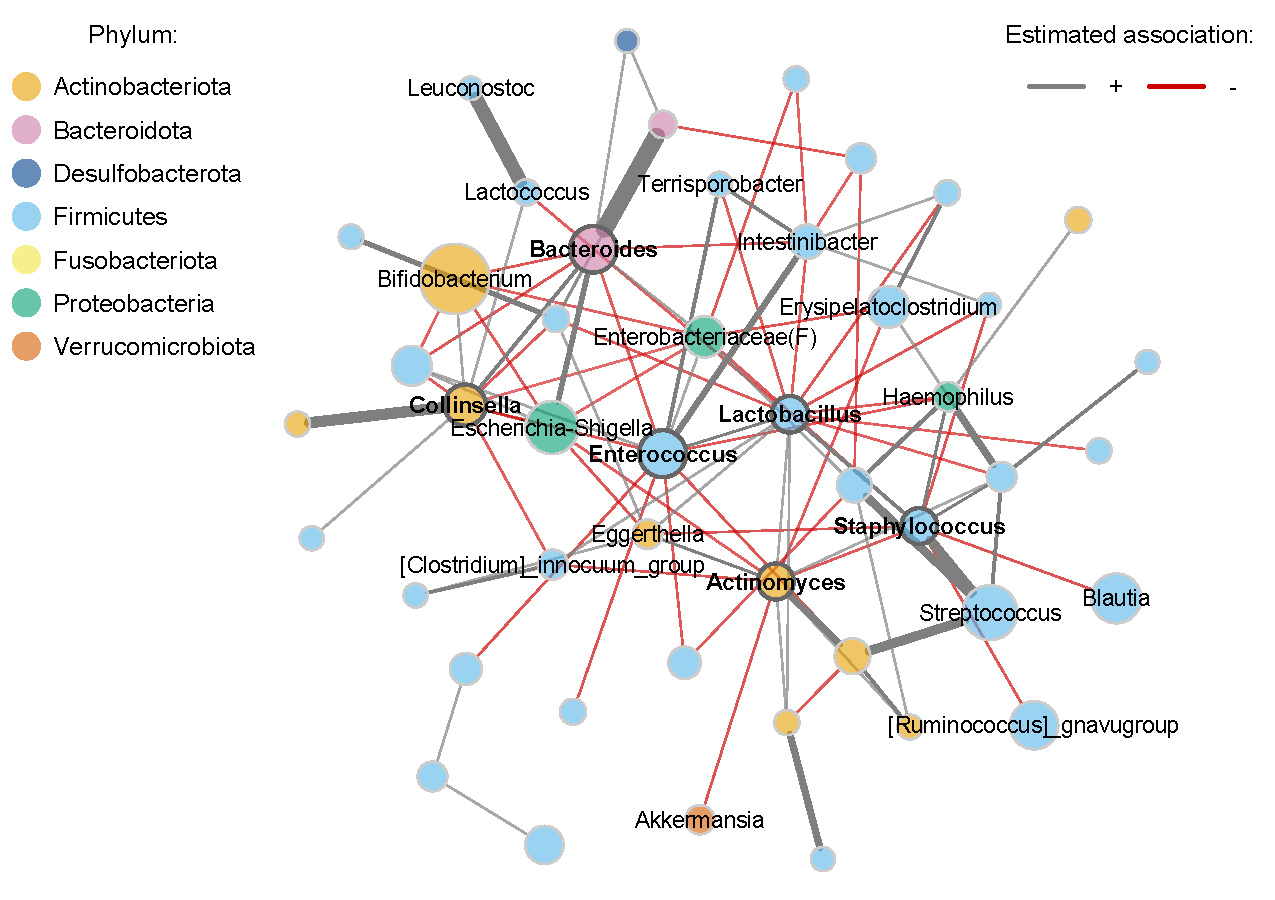
\includegraphics[width=\textwidth]{../ch07_application/figures/10_network_analysis/single_net_plot_slr_slrlay-1.pdf}
\caption{\textbf{SPIEC-EASI SLR association network with spring layout.} The network was estimated from the complete default data set using the SPIEC-EASI sparse-plus-low-rank (SLR) approach with the rank selected by the Bayesian information criterion, as described in Section~\ref{sec:7app:network:sensitivity}. Nodes represent genera and are colored according to phylum, while node sizes are proportional to the mean CLR coordinate across samples. Gray and red edges indicate positive and negative estimated conditional associations, respectively. Node positions were determined by a force-directed layout based on the sparse-plus-low-rank network itself. Labels identify genera highlighted in the preceding abundance, differential abundance, or differential distribution analyses, as well as selected highly connected genera.}
\label{fig:app:7app:net_single_slr}
\end{figure}

\begin{figure}[H]
\centering
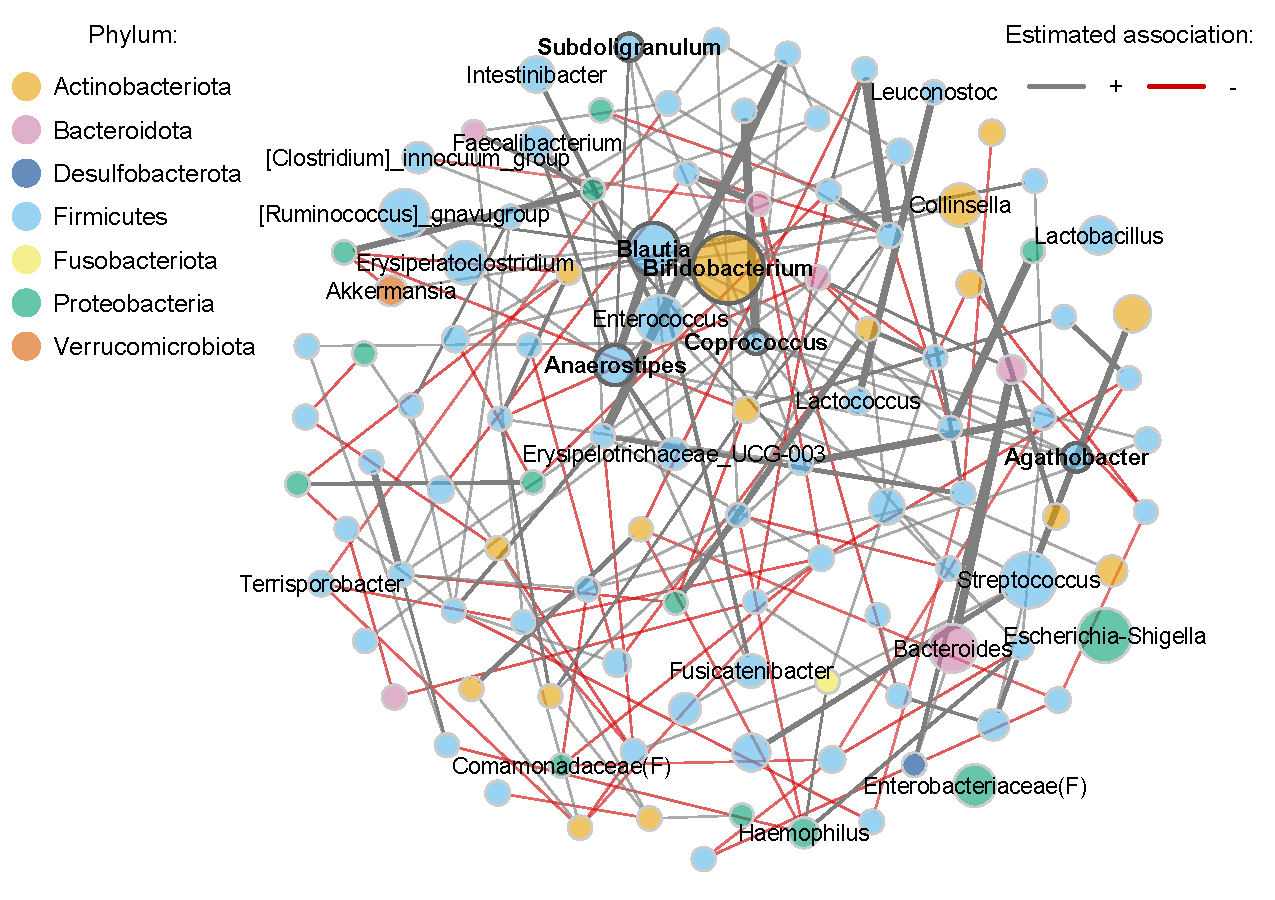
\includegraphics[width=\textwidth]{../ch07_application/figures/10_network_analysis/single_net_plot_spring_ownlay-1.pdf}
\caption{\textbf{SPRING association network with spring layout.} The network was estimated from the complete default data set using SPRING with the StARS settings described in Section~\ref{sec:7app:network:sensitivity}. Nodes represent genera and are colored according to phylum, while node sizes are proportional to the mean mCLR coordinate across samples. Gray and red edges indicate positive and negative estimated conditional associations, respectively. Node positions were determined by a force-directed layout based on the SPRING network itself. Labels identify genera highlighted in the preceding abundance, differential abundance, or differential distribution analyses, as well as selected highly connected genera.}
\label{fig:app:7app:net_single_spring}
\end{figure}

%====================================
\section{Network comparison}
\label{sec:app:7app:net_compare}
%====================================

\begin{figure}[H]
\centering
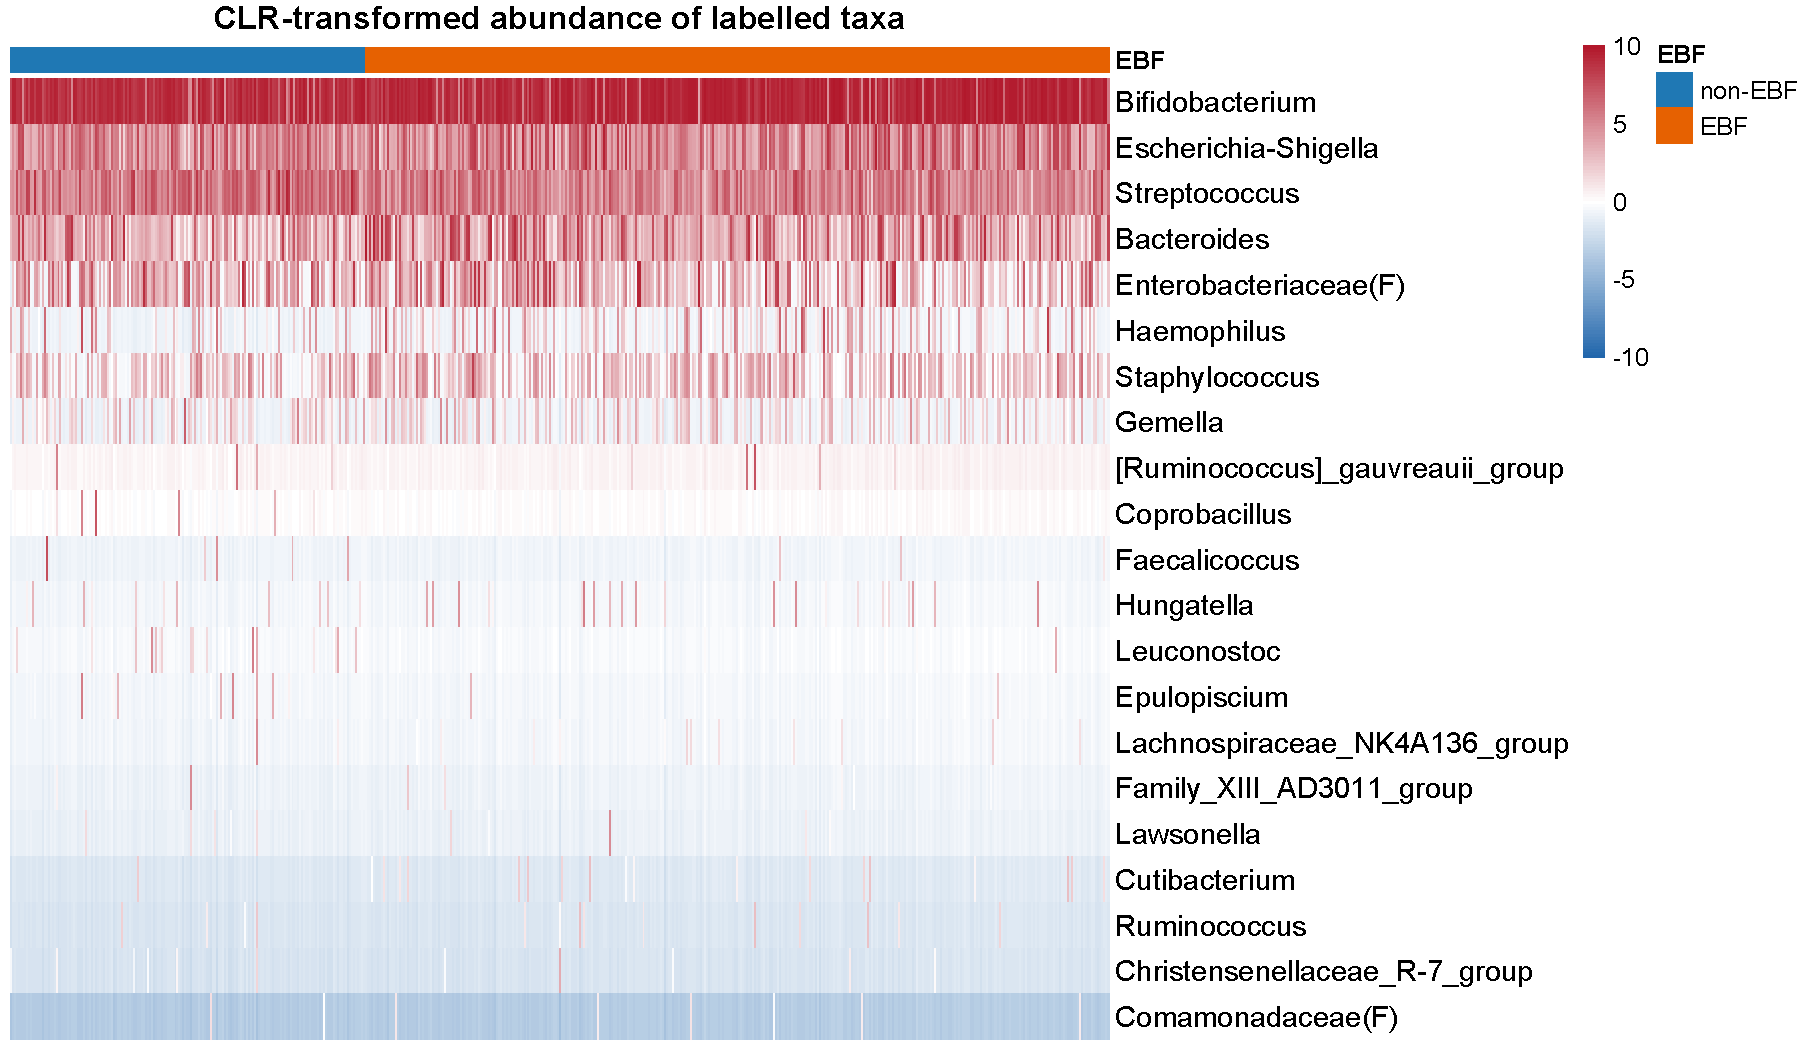
\includegraphics[width=\textwidth]{../ch07_application/figures/11_network_comparison/thesis_labelled_taxa_clr_heatmap-1.pdf}
\caption{\textbf{CLR-transformed abundances of selected genera.} The heatmap shows CLR coordinates after Bayesian-multiplicative replacement for the genera highlighted in Figure~\ref{fig:7app:network:ebf_network}. Columns represent samples and rows represent genera. Samples are ordered by EBF group. The transformed values form the fixed sample representation used for correlation-shrinkage network estimation in the differential network and differential association analyses.}
\label{fig:app:7app:net_compare_clr_heatmap}
\end{figure}

\begin{figure}[H]
\centering
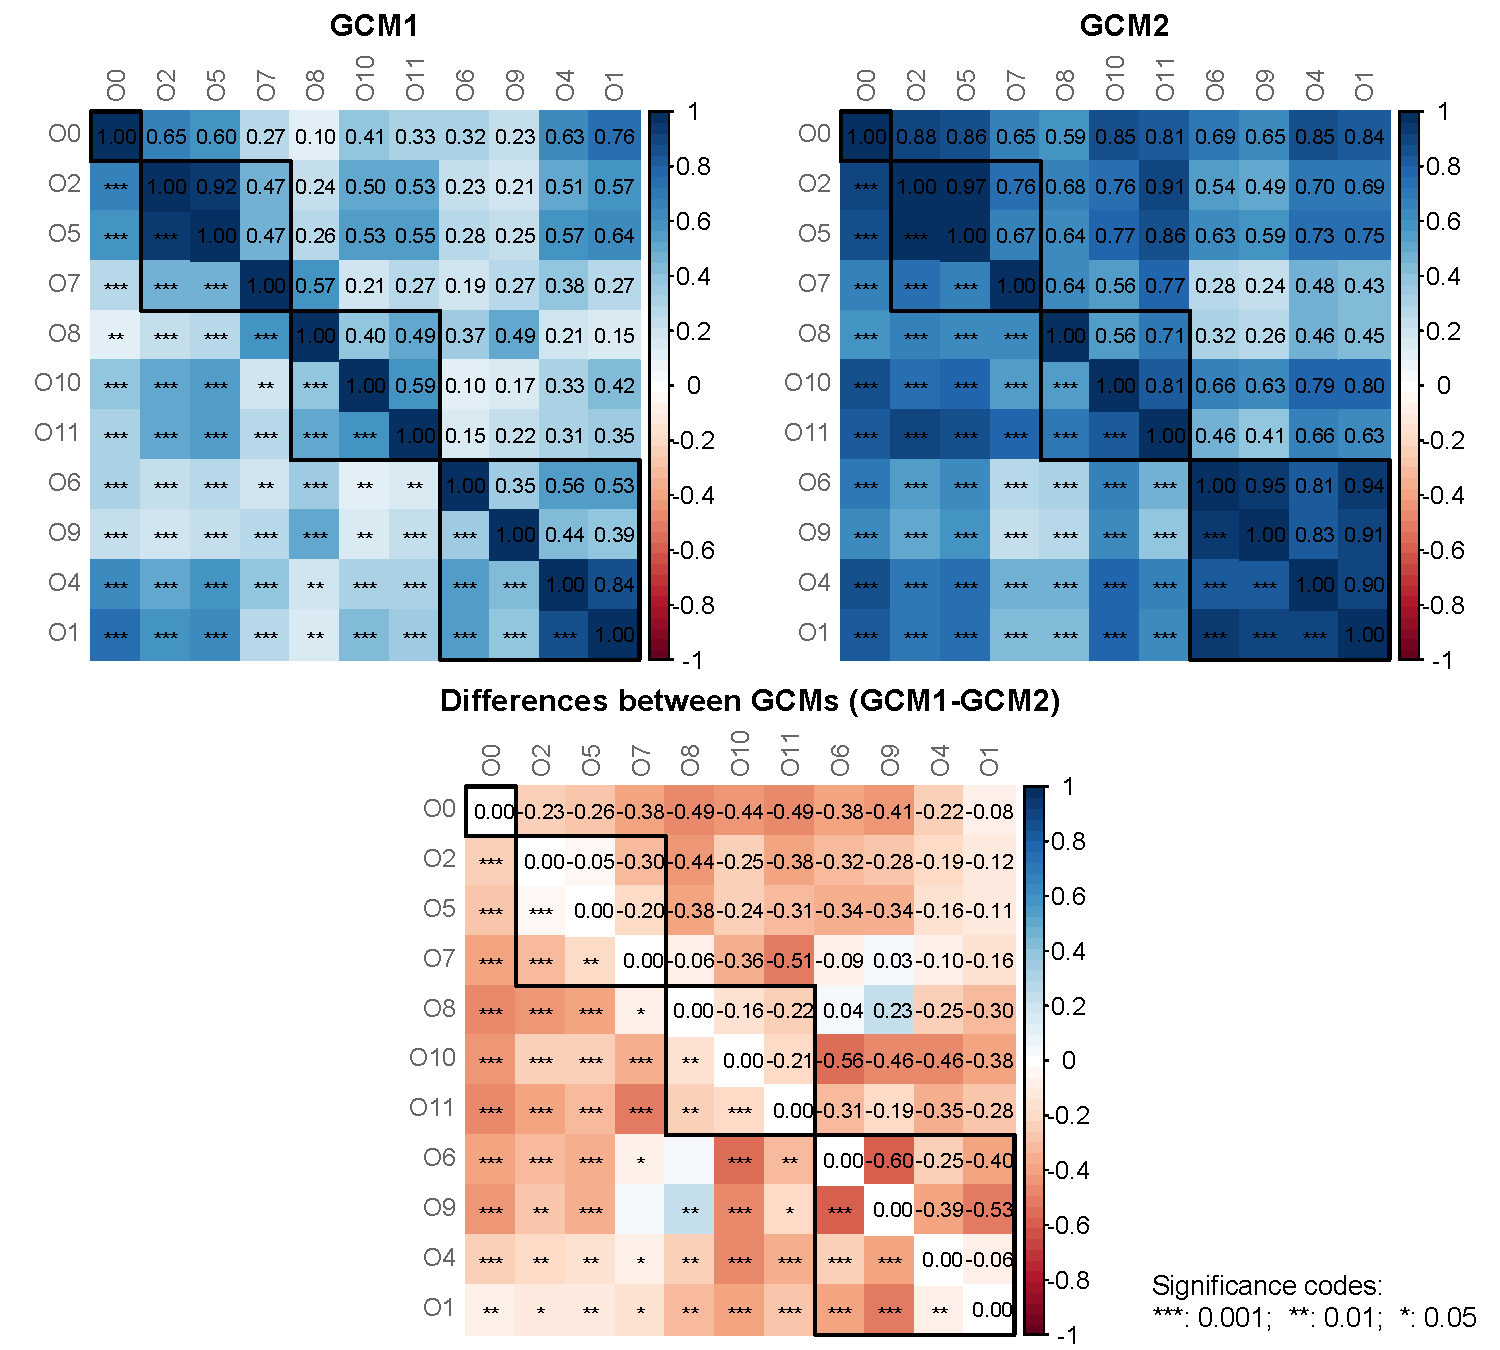
\includegraphics[width=\textwidth]{../ch07_application/figures/11_network_comparison/ebf_corshrink_bayesMult_gcm-1.pdf}
\caption{\textbf{Graphlet correlation matrices for the two EBF groups.} The upper panels show the graphlet correlation matrices (GCMs) of the correlation-shrinkage networks estimated after Bayesian-multiplicative replacement for children with EBF duration $=0$ and EBF duration $\geq 2$, respectively. Entries represent Spearman correlations between the non-redundant graphlet-orbit counts defined in Section~\ref{sec:5net:net_analysis:graphlets}. The lower panel displays the element-wise difference between the two matrices, computed as GCM$_{\mathrm{EBF}=0}$ minus GCM$_{\mathrm{EBF}\geq2}$. Asterisks indicate the significance level of the corresponding Fisher test.}
\label{fig:app:7app:net_compare_gcm}
\end{figure}

% !TeX root = ../thesis.tex
\chapter{Electronic appendix}
\label{app:electronic-appendix}

The electronic appendix is provided as a version-controlled GitHub repository archived on Zenodo \citep{Peschel2026thesisRepo}. The repository contains the code, analysis material, and figures accompanying this thesis and is organized according to the chapter structure of the dissertation. Each thesis chapter is represented by a corresponding folder. For chapters involving computational analyses, these folders contain the scripts and material used to generate the reported results, tables, and figures. For chapters without accompanying analysis scripts, the corresponding folders contain the overview figures and other graphical material shown in the thesis.

The repository contains the material required to reproduce the computational results reported in this thesis. Some large simulated data files are not archived to keep the repository size manageable. For analyses depending on such files, the corresponding chapter folder should be rerun from its first script before executing subsequent analysis scripts. Depending on the analysis, regenerating simulated data and rerunning downstream scripts may require substantial computation time.
% !TeX root = ../thesis.tex
%%%%%%%%%%%%%%%%%%%%%%%%%%%%%%%%%%%%%%%%%%
% Eidesstattliche Versicherung
%%%%%%%%%%%%%%%%%%%%%%%%%%%%%%%%%%%%%%%%%%
\cleardoublepage
\thispagestyle{empty}

\vspace*{2.2cm}

{\Large\bfseries
Eidesstattliche Versicherung (Affidavit)\par}

\vspace{0.4cm}

{\normalsize
(Siehe Promotionsordnung vom 12.\ Juli 2011, \S\,8 Abs.\ 2 Pkt.\ 5)\par}

\vspace{1.5cm}

\noindent
Hiermit erkläre ich an Eides statt, dass die Dissertation von mir selbstständig, ohne unerlaubte Beihilfe angefertigt ist.

\vspace{1.5cm}

\noindent
München, den 07.07.2026
\hfill
\begin{minipage}[t]{0.36\textwidth}
  \centering
  \rule{\textwidth}{0.4pt}\\[-0.1cm]
  Stefanie Peschel
\end{minipage}

\vspace*{1.8cm}

\end{document}